%%%%%%%%%%%%%%%%%%%%%%%%%%%%%%%%%%%%%%%%%%%%%%%%%%%%%%%%%%%%%%%%%%%%%%%%%%%%
%                                                                          %
% This is the LaTeX source of a Project Gutenberg eBook, online at         %
% https://www.gutenberg.org. Please find the license for this eBook at     %
% https://www.gutenberg.org/license                                        %
%                                                                          %
%%%%%%%%%%%%%%%%%%%%%%%%%%%%%%%%%%%%%%%%%%%%%%%%%%%%%%%%%%%%%%%%%%%%%%%%%%%%
%%%%%%%%%%%%%%%%%%%%%%%%%%%%%%%%%%%%%%%%%%%%%%%%%%%%%%%%%%%%%%%%%%%%%%%%%%%%
%                                                                          %
% Producer's Comments:                                                     %
%                                                                          %
% Use lualatex so we can have modern fonts.                                %
% This volume contains a variant beta which is available in stix2          %
% Volume 1 contains a capital Upsilon. In stix2 this is                    %
% indistinguishable from roman Y so use 'Latin Modern Math' for capital    %
% greek letters so capital Upsilon has curved arms.                        %
%                                                                          %
% Compile sequence:                                                        %
% latexmk -lualatex <filename>                                             %
%                                                                          %
% No overfull hboxes                                                       %
% 7 underfull hboxes                                                       %
%                                                                          %
% To avoid many overfull hboxes in lines with in-line maths allow more     %
% inter-word spacing using emergencystretch 4.5em.                         %
% This results in many underfull hboxes, suppress the warnings for most    %
% of these using hbadness=5000. Only the worst remain.                     %
%                                                                          %
% The page size is similar to octavo like the original. There are          %
% generally more text words per line than the original. Display math is    %
% similar to original but in a few cases expressions have been split or    %
% combined to fit the width. The original 'condensed intertext' has not    %
% been implemented.                                                        %
%                                                                          %
%%%%%%%%%%%%%%%%%%%%%%%%%%%%%%%%%%%%%%%%%%%%%%%%%%%%%%%%%%%%%%%%%%%%%%%%%%%%

\listfiles
\documentclass[12pt,oneside]{book}[2021/10/04]

\usepackage{unicode-math}[2020/01/31]
\usepackage{mathtools}[2021/02/02] %% for multlined and shortintertext
\usepackage{enumitem}[2019/06/20] % for index items

% stix2 has a variant beta
\setmainfont{STIX Two Text}
\setmathfont{STIX Two Math}
\newfontfamily\gfont{QTCloisteredMonk}

% stix2 Upsilon looks like Y
\setmathfont[range=up/{Greek}]{Latin Modern Math}

\setlength{\paperwidth}{14.87cm}%
\setlength{\paperheight}{21.02cm}%

\usepackage[
  top=0.8cm,
  bottom=0.5cm,
  left=0.81cm,
  right=0.81cm,
  headheight=17pt, % as per the warning by fancyhdr
  includehead,includefoot,
  heightrounded, % to avoid spurious underfull messages
]{geometry}[2020/01/02]% Page Geometry

\usepackage[skip=5pt plus1pt, indent=1.5em]{parskip}[2021-03-14] % parskip adjustments

\usepackage{fancyhdr}[2019/01/31] % for page headers

\usepackage{graphicx}[2021/09/16] % for images and scalebox
\graphicspath{ {./images/} }
\usepackage{letterspace}[2021/12/10] % letterspacing - \textls
\usepackage{scalerel}[2016/12/29] % scaling and stretching of objects
\usepackage{nowidow}[2011/09/20] % 1.0 Easily prevent widows and orphans
\usepackage[
  pdfpagelayout=SinglePage,
  pdfdisplaydoctitle,
  colorlinks=true,
  linkcolor=blue,
]{hyperref}[2021-06-07] % Hypertext links for LaTeX

\def\scaleint#1{\vcenter{\hbox{\scaleto[2.5ex]{\displaystyle\int}{#1}}}}
\newcommand{\bigint}{\scaleint{7ex}}

% redefine as mathord instead of mathbin
\DeclareMathSymbol{·}{\mathord}{symbols}{"00B7}

\renewcommand{\headrulewidth}{0pt}

\newcommand{\Chapter}[1]{
  \newpage
  \thispagestyle{empty}
  \begin{center}
  \Large
  {#1}\\
  \vspace*{0.6cm}
  \end{center}
}

\newcommand{\Runhead}[1]{
  \fancyhead[C]{#1}
}

\newcommand{\Subhead}[1]{
  \begin{center}
  {#1}
  \end{center}
}

\newcommand{\Section}{\vspace{1.2ex}}

\newenvironment{squote}{\par\small}{\par}

%% extra space for display math inline
\newcommand{\xp}{\vrule height 3.4ex depth 2.4ex width 0pt}
\newcommand{\xxp}{\vrule height 3.9ex depth 2.8ex width 0pt}
\def\mystrut(#1,#2){\vrule height #1ex depth #2ex width 0pt}

\newcommand{\bigsurd}{\sqrt{\vphantom{\dfrac{a}{b}}}}
\newcommand{\bbigsurd}{\sqrt{\vphantom{\dfrac{A}{B}}}}
\newcommand{\ldot}{\,.\,}

\newcommand{\oldfactorial}[1]{\mathpalette\oldfactorialaux{#1}}
\newcommand{\oldfactorialaux}[2]{%
  {#1\mkern1mu\oalign{\vrule\,$#1#2\mathstrut$\,\cr\noalign{\hrule}}}}

% to align columns of numbers
\newcommand{\intspace}{\hphantom{0}}

\newcommand{\longbar}[1]{
  \rule{\widthof{#1}}{1pt}\\
  #1
}

% Unicode does not define an italic variant beta in Mathematical alphanumeric symbols
\newcommand{\varbeta}{\mathit{\symbol{"03D0}}}
\newcommand{\invprime}{\rotatebox[origin=c]{180}{\prime}}

% smaller surd symbol
\newcommand{\xsurd}{\scaleobj{0.8}{\surd}}
% for root -1, space before
\newcommand{\xsurdm}{\,\xsurd}

\newenvironment{indexletter}
{\begin{description}[noitemsep, labelwidth=1em]}
{\end{description}
}

% To avoid overfull hboxes with in-line expressions allow more inter-word spacing
\emergencystretch 4.5em%
% suppress most resulting underfull hboxes
\hbadness=5000

\hyphenation{spher-oids ré-ci-proque}


\usepackage{fontspec}[2022/01/15] % for font selection
\usepackage{array}[2021/10/04] % for >{\raggedright\arraybackslash} in tabular
\usepackage{fancyhdr}[2019/01/31] % for page headers
\usepackage{graphicx}[2021/09/16] % for images and scalebox
\usepackage{hyperref}[2021-06-07] % Hypertext links for LaTeX

\graphicspath{ {./images/} }

% for PG text use a sans font similar size to stix2, some others are much bigger
\newfontfamily\pgfont{Alegreya Sans}
\newenvironment{PGtext}{\thispagestyle{empty}
\raggedright \pgfont
\setlength\parskip{5pt plus1pt}}{}

\newcommand{\PGLicense}{%
  \clearpage
  \pagestyle{fancy}
  \fancyhf{}
  \pagenumbering{Roman}
  \fancyhead[L]{}
  \fancyhead[C]{\small \pgfont License}
  \fancyhead[R]{\thepage}
  \renewcommand{\headrulewidth}{0pt}
}

\newcommand{\LicenseSection}[1]{\subsection*{\pgfont\normalsize\bfseries #1}}

\begin{document}
\hypersetup{
    pdftitle={A history of the mathematical theories of attraction and the figure of the earth from the time of Newton to that of Laplace. Volume 2},
    pdfauthor={Isaac Todhunter},
    pageanchor=false,
    pdfdisplaydoctitle=true,
    colorlinks=true,
    urlcolor=blue,
}

\newgeometry{ % let image fill page
  top=0cm,
  bottom=0cm,
  left=0cm,
  right=0cm,
}
\thispagestyle{empty}
\begin{figure}[tbp]
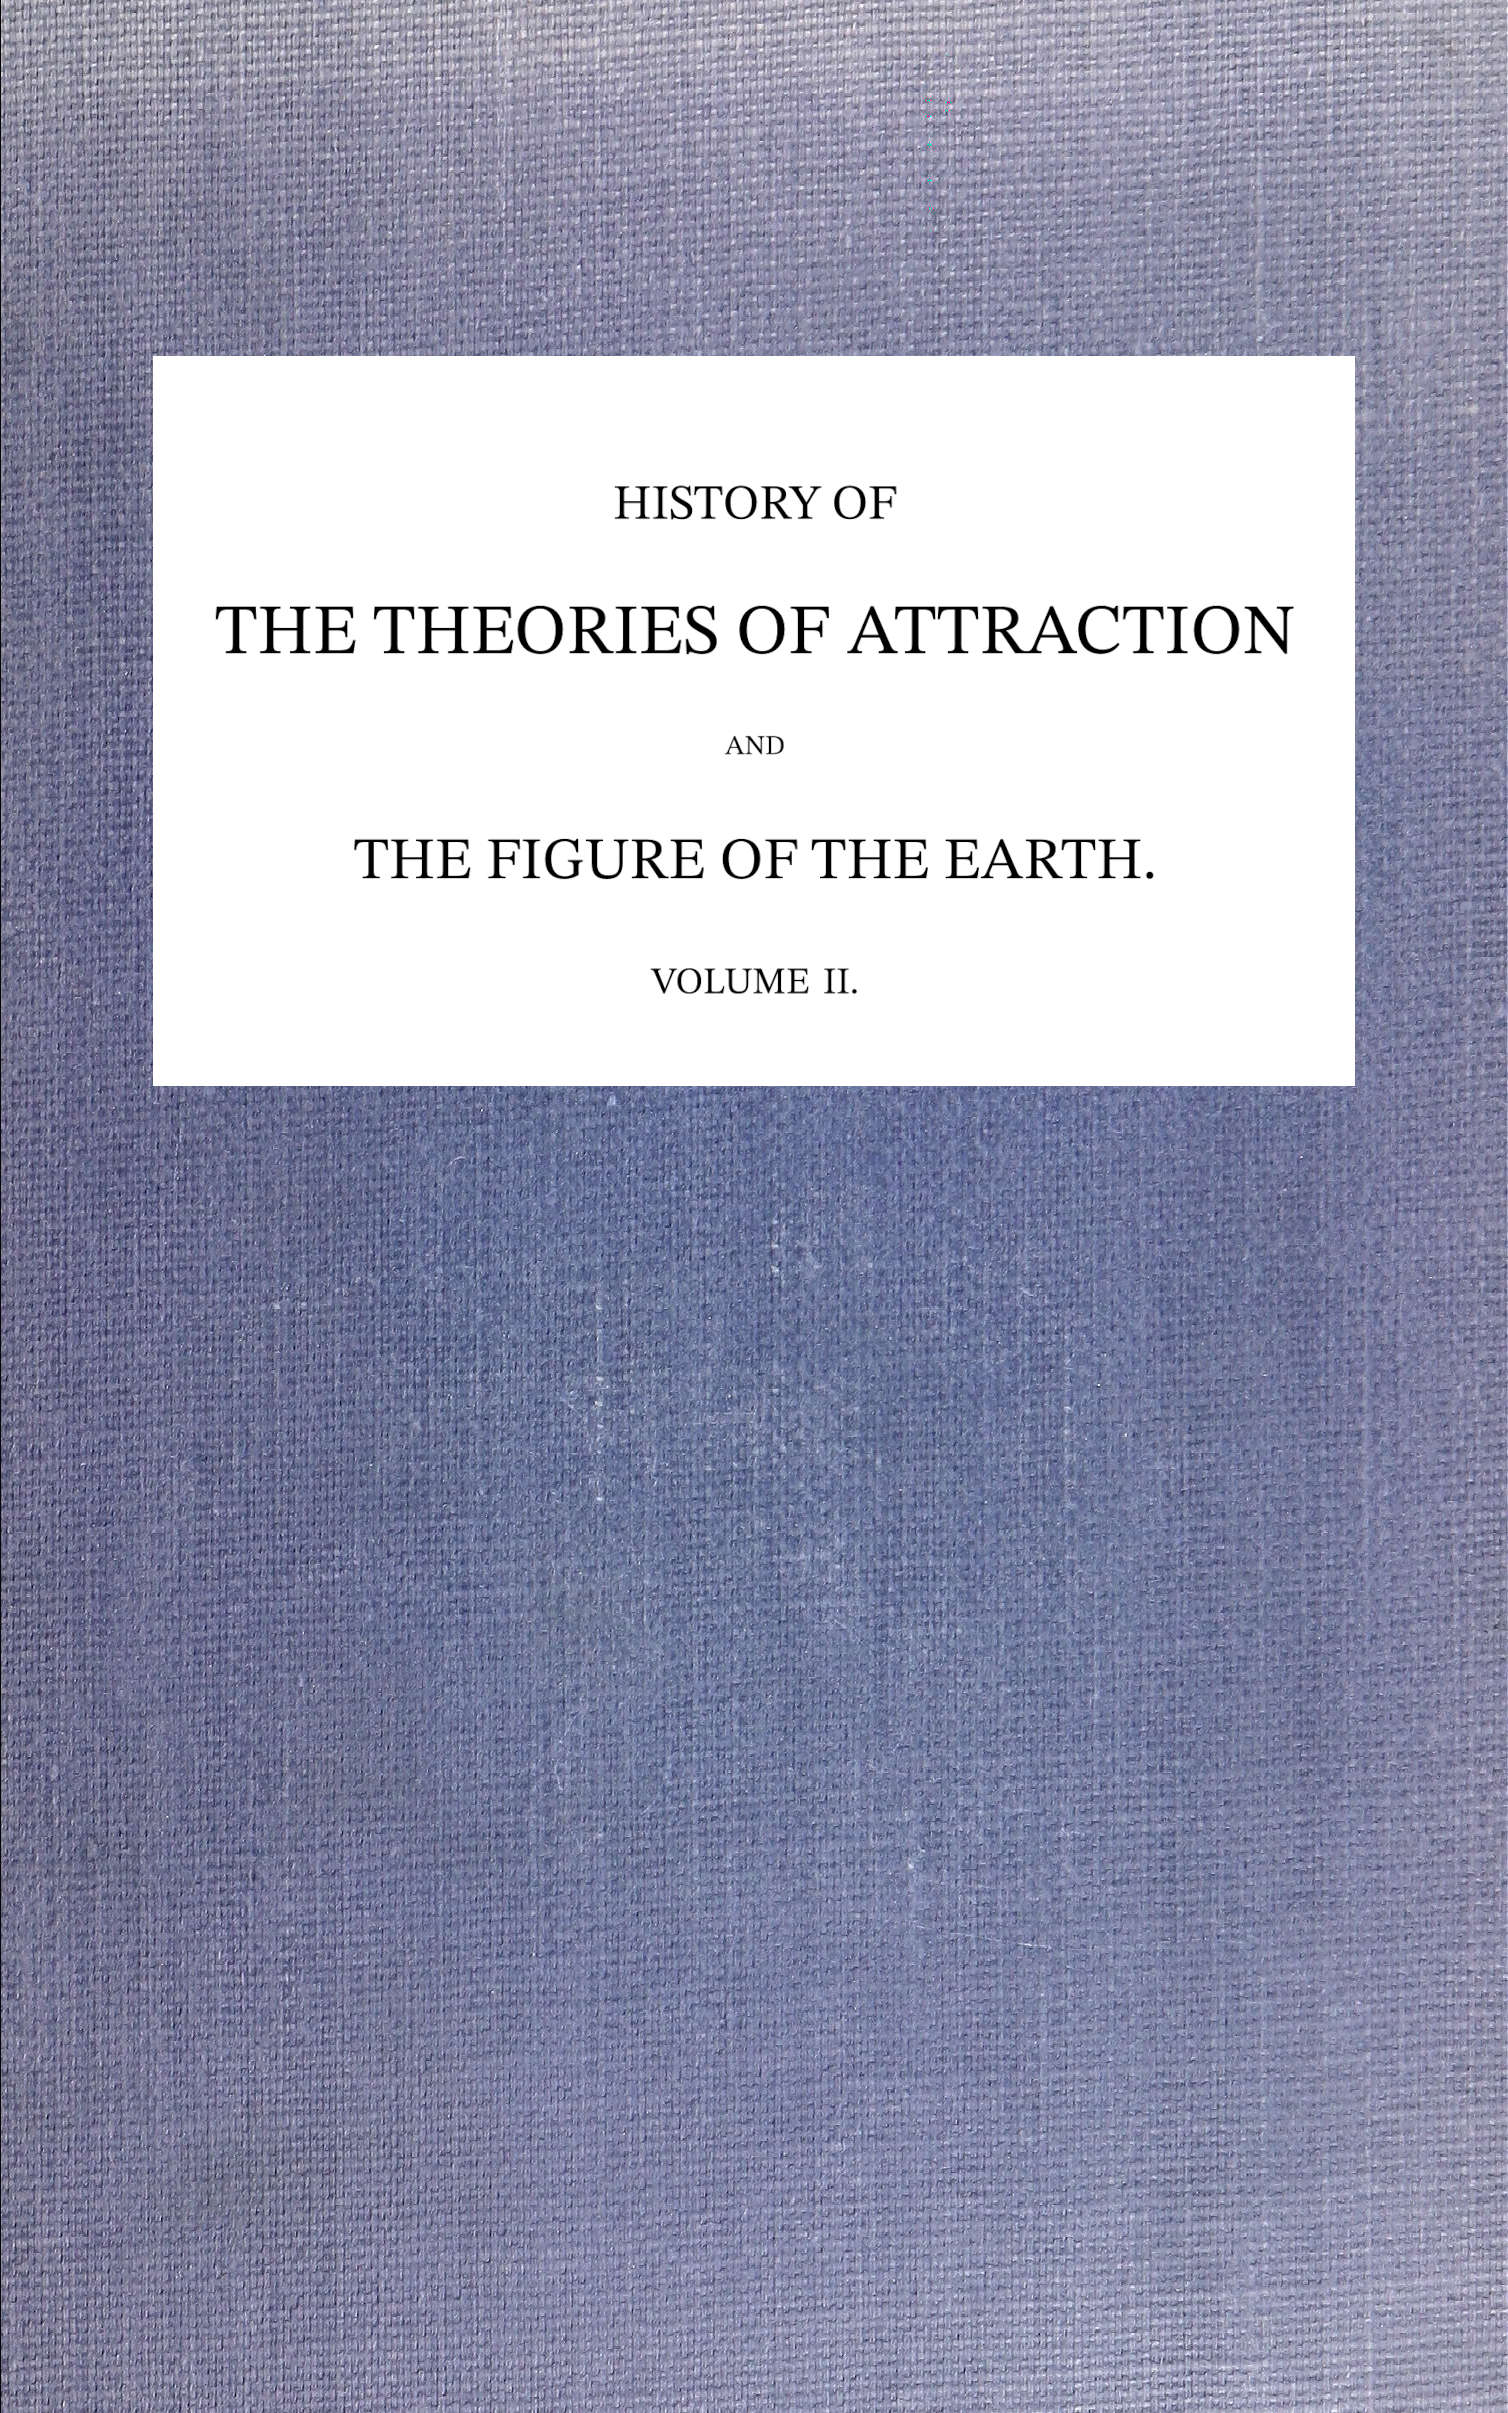
\includegraphics[width=0.999\textwidth,height=0.999\textheight,keepaspectratio]{cover.jpg}
\centering
\end{figure}
\restoregeometry

\newpage
\begin{PGtext}
\begin{center}
\large
\textbf{
The Project Gutenberg eBook of A history of the mathematical theories of attraction and the figure of the earth from the time of Newton to that of Laplace. Volume 2 by Isaac Todhunter
}
\end{center}
\InputIfFileExists{pgheader.tex}{}{}
\renewcommand*{\arraystretch}{1.5}
\begin{tabular}{p{2.5cm}>{\raggedright\arraybackslash}p{\dimexpr \linewidth-3.5cm}}
Title: &        A history of the mathematical theories of attraction and the figure of the earth from the time of Newton to that of Laplace. Volume 2\\
Author: &       Isaac Todhunter\\
Release Date: & January 18, 2023 [eBook \#69832]\\
Language: &     English\\
Credits: & The Online Distributed Proofreading Team at https://www.pgdp.net (This file was produced from images generously made available by The Internet Archive)\\
\end{tabular}
\vfill
\begin{center}
*** START OF THE PROJECT GUTENBERG EBOOK A history of the mathematical theories of attraction and the figure of the earth from the time of Newton to that of Laplace. Volume 2 ***
\end{center}
\end{PGtext}

\pagestyle{fancy}
\fancyhf{}
\fancyhead[R]{\thepage}

\frontmatter
\fontdimen2\font=0.75ex% inter word space
\textit{\fontdimen2\font=0.75ex}
{\small{\fontdimen2\font=0.75ex}}
%%-----File: 001.png-----%%
\thispagestyle{empty}
\hspace{0pt}
\vfill
\begin{center}
\large
HISTORY OF\\[0.5cm]
\LARGE
THE THEORIES OF ATTRACTION\\[0.7cm]
\scriptsize
AND\\[0.5cm]
\Large
THE FIGURE OF THE EARTH.\\[0.7cm]
\small
VOLUME II.
\vfill
\end{center}
%%-----File: 002.png-----%%
\newpage
\thispagestyle{empty}
\hspace{0pt}
\vfill
\small
Si Poisson a été d'une fécondité extraordinaire, c'est qu'il était au courant
de ce qui avait été fait avant lui, au courant, par exemple, des immenses
travaux des Euler et des d'Alembert; c'est qu'il ne s'est jamais sottement
obstiné à perdre son temps et ses forces à la recherche de ce qui était
déjà trouvé.

Que l'exemple de Poisson serve de leçon à ces esprits irréfléchis qui, sous le
prétexte de conserver leur originalité, dédaignent de prendre connaissance des
découvertes de leurs devanciers, et restent sur les premiers dégrés de l'échelle,
tandis que, avec moins d'orgueil, ils se seraient élevés au sommet.

\hspace*{\fill}
\textsc{Arago}, \textit{Œuvres Complètes}, Tome \textsc{ii}.\ page 656.
\hspace{1cm}
\vfill
%%-----File: 003.png-----%%
\newpage
\thispagestyle{empty}
\begin{center}
\large
\textls[200]{A HISTORY}\\ [0.6cm]
\scriptsize
OF THE\\[0.5cm]
\LARGE
\scalebox{.8}[1.0]{MATHEMATICAL THEORIES OF ATTRACTION}\\ [0.7cm]
\scriptsize
AND\\ [0.5cm]
\Large
THE FIGURE OF THE EARTH,\\ [1cm]
\normalsize
\textit{FROM THE TIME OF NEWTON TO THAT\\
OF LAPLACE.}\\ [2cm]
\scriptsize
BY\\ [0.4cm]
\large
I. TODHUNTER, M.A., F.R.S.\\ [1.2cm]
\normalsize
\textit{IN TWO VOLUMES.}\\[0.4cm]
VOLUME II.\\ [1.3cm]
{\large\gfont{London:}}\\[0.2cm]
\textls[150]{MACMILLAN AND CO}.\\[0.2cm]
1873.\\[0.4cm]
{[}\textit{All Rights reserved.}{]}
\end{center}
%%-----File: 004.png-----%%
\newpage
\thispagestyle{empty}
\hspace{0pt}
\vfill
\begin{center}
{\large\gfont{Cambridge:}}\\[0.2cm]
\scriptsize
PRINTED BY C. J. CLAY, M.A.\\[0.2cm]
AT THE UNIVERSITY PRESS.
\end{center}
\vfill
%%-----File: 005.png-----%%
\mainmatter
\normalsize
\Chapter{CHAPTER XIX}
\Subhead{LAPLACE'S FIRST THREE MEMOIRS.}
\Runhead{\textsc{laplace's first memoir.}}

\Section
741. \textsc{The} investigations of Laplace on Attractions and the
Figure of the Earth fall naturally into five divisions. The first
division consists of three memoirs, which treat the subjects
without the use of what we now call the \textit{Potential Function}, or of
that branch of analysis which we now call \textit{Laplace's Functions}.
The second division consists of a separate volume which uses the
Potential Function. The third division consists of various memoirs
which use both the Potential Function and Laplace's Functions.
The fourth division is formed by the republication of the
preceding researches in the first and second volumes of the
\textit{Mécanique Céleste}. The fifth division consists of researches subsequent
to the publication of the second volume of the \textit{Mécanique
Céleste}; they are reproduced in the fifth volume of the \textit{Mécanique
Céleste}.

We shall consider in the present Chapter Laplace's first three
memoirs.

\Section
742. We begin with the seventh volume of the \textit{Mémoires de
Mathématique \dots\ par divers Savans} \dots\ 1773: the date of publication
is 1776. This volume contains two memoirs by Laplace,
which among other subjects treat largely of Probability: see
pages 473\dots 475 of my \textit{History \dots\ of Probability}. The part of the
volume with which we are now concerned is entitled \textit{Sur la figure
de la Terre}; it occupies pages 524\dots 534. It is not stated when
these investigations were sent to the Academy; but from the
title of the volume in which they appear we see that Laplace
was not a member of the Academy when they were sent.
%%-----File: 006.png-----%%

\Section
743. Laplace begins thus on page 524:
\begin{squote}
Lorsque Newton voulut déterminer la figure de la Terre, il considéra
cette Planète comme une masse fluide homogène, et il supposa
que la figure qu'elle a prise en vertu de son mouvement de rotation est
celle d'un sphéroïde elliptique. Cette supposition étoit fort précaire;
les Géomètres en ont ensuite démontré la possibilité; mais si la figure
nécessaire pour l'équilibre, au lieu d'être elliptique, eût été d'un autre
genre, on auroit été fort embarrassé pour la déterminer, parce qu'il est
beaucoup plus facile de s'assurer si une figure donnée convient à l'équilibre,
que de chercher immédiatement celles qui peuvent y convenir.
Ce dernier Problème est sans contredit un des points les plus intéressans
du Système du Monde; voici quelques recherches qui y sont relatives.
\end{squote}

\Section
744. Thus the following is the problem to be discussed: a
mass of homogeneous fluid in the form of a figure of revolution
nearly spherical rotates with uniform angular velocity round its
axis of figure and remains in relative equilibrium; determine the
form. I call this problem Legendre's, because he was the first
to solve it with tolerable success.

\Section
745. Let there be a circle of radius unity; let \(\psi\) be the angle
which the radius to any point makes with a fixed radius: so that
the ordinate of this point is \(\sin \psi\). Produce this ordinate until
it becomes \(\sin\psi + \xp\dfrac{\alpha y}{\sin\psi}\), where \(\alpha\) is very small, and \(y\) is some
function of \(\psi\). Put \(x\) for \(\cos\psi\). Then Laplace arrives at a
differential equation between \(y\) and \(x\) of an infinite order, to
determine the required generating curve; that is a differential
equation involving \(\xp\dfrac{d^2y}{dx^2}\), \(\xp\dfrac{d^3y}{dx^3}\), \dots\ and so on \textit{ad infinitum}.

\Section
746. The preceding notation does not look very promising;
in fact Laplace does not explicitly start with it, but arrives at it
as he proceeds. Unless \(y\) is very small when \(\psi\) is very small the
process is not satisfactory. Moreover Laplace in order to form his
differential equation expands a function into a series without discussing
whether the series is convergent.
%%-----File: 007.png-----%%

\Section
747. The main result at which he arrives deserves notice.
He wishes to know whether equilibrium would subsist for any
other form besides an exact sphere when there is no rotation.
He cannot completely solve this problem; but he shews that \(y\)
cannot consist of a series of the form \(ax^{\lambda} + bx^{\mu} + cx^{\nu} + \ldots\), where
\(\lambda\), \(\mu\), \(\nu\), \dots\ are numbers in \textit{descending} order of magnitude. That
is \(y\) cannot consist of a \textit{finite} number of terms each involving a
power of \(x\); nor can \(y\) be an infinite series of \textit{descending} powers
of \(x\): but he does not shew that \(y\) cannot be an infinite series of
\textit{ascending} powers of \(x\).

When the fluid is supposed to rotate Laplace's demonstration
amounts to shewing that among all series, finite or infinite, which
can be arranged in descending powers of \(x\), the only admissible
form of \(y\) is \(ax^2 + bx + c\); where \(a\), \(b\), and \(c\) are constants.

\Section
748. Laplace's demonstration is difficult, but satisfactory;
that is to say after the points to which we have drawn attention
in Art.\ 746, no very serious objection will occur to a reader.

After finishing his demonstration, Laplace says on his page 534:
\begin{squote}
\dots\ Je dois observer ici que M. d'Alembert a déjà fait une remarque
semblable pour le cas où les exposans de \(x\) sont des nombres entiers et
positifs (\textit{voyez le tome} V \textit{des Opuscules} de ce grand Géomètre).
\end{squote}

These words are quite consistent with the supposition, that
Laplace had found the error which we have pointed out in
D'Alembert's process; because \textit{to make a remark} is far less than
\textit{to demonstrate}. See Art.\ 576.

\Section
749. Laplace concludes with these words:
\begin{squote}
Il seroit utile d'étendre ces recherches au cas où les couches de la
masse fluide sont inégalement denses; c'est ce que je me propose de
faire dans un autre Mémoire.
\end{squote}

The intention here expressed was not carried into effect until
the publication of Laplace's seventh memoir in the Paris \textit{Mémoires}
for 1789.

\Section
750. All that Laplace's first memoir contains on our subject
is reproduced with better notation in his second memoir to which
%%-----File: 008.png-----%%
we shall proceed in our next Article: it is therefore unnecessary
to treat the first memoir with much detail. In the second memoir
we shall find that the radius vector of the generating curve is
denoted by \(1 + \alpha f(\cos\psi)\), where \(\alpha\) is very small; so that what was
called \(\sin\psi + \xp\dfrac{\alpha y}{\sin\psi}\) in Art.\ 745 is equal to the \(\sin\psi \{1 + \alpha f(\cos\psi)\}\)
of the second memoir: that is \(\xp\dfrac{y}{\sin\psi}\) of the first memoir is
\(\sin\psi f(\cos\psi)\) of the second memoir, or \(y\) of the first memoir
is \(\sin^2\psi f(\cos\psi)\) of the second memoir. In the second memoir
\(y\) is put for \(f(\cos\psi)\).

\Runhead{\textsc{laplace's second memoir.}}
\Section
751. In the Paris \textit{Mémoires} for 1772, \textit{Seconde Partie}, published
in 1776, we have a memoir by Laplace entitled \textit{Recherches sur le
Calcul Intégral et sur le Système du Monde}; at a later part of
the volume there are some \textit{Additions} to this memoir: among
these Additions we have a section entitled \textit{De l'Équilibre des
Sphéroïdes homogènes}, which occupies pages 536\dots 554 of the
volume.

\Section
752. The problem proposed to be discussed is the same as that
of the preceding memoir: see Art.\ 744. Laplace was not able
to solve the problem completely; but he reproduced his former
demonstration, somewhat improved, that for a large number of
figures the relative equilibrium was impossible.

\Section
753. But although he did not in this memoir arrive at the necessary
form for equilibrium, yet he obtained a very remarkable
result: namely, that the law of the variation of gravity, whatever be
the form of equilibrium, is the same as for an oblatum. We will
give in substance the method by which Laplace obtains this result.

We may remark that Laplace investigates the polar expression
for an element of mass, namely in the usual modern notation
\(r^2 dr \sin\theta\,d\theta\,d\phi\): see his page 539. The investigation is in fact
the same as we now have in our elementary books: see \textit{Integral
Calculus}, third edition, Art.\ 207.

In his first memoir Laplace used this polar expression but did
not investigate it; he merely says, ``on trouvera facilement\dots'':
see his page 525. See also Art.\ 710.
%%-----File: 009.png-----%%

\Section
754. Let there be a curve differing very little from a circle,
and symmetrical with respect to a diameter. Let half the length
of this diameter be unity, and let the length of a radius vector
inclined at an angle \(\psi\) to the diameter be \(1 + \alpha f(\cos\psi)\), where \(f\)
denotes any function, and \(\alpha\) is a very small quantity the square
of which we shall neglect. Suppose a solid formed by the revolution
of this curve round the diameter which divides it symmetrically;
take this diameter for the direction of the axis of \(x\): then
the equation to the surface will be
\[\xsurd(x^2+y^2+z^2) = 1 + \alpha f \left\{ \frac{x}{\xsurd(x^2+y^2+z^2)}\right\}\tag{1}.\]

We propose to find the attraction of the solid at a point
situated on its surface; this point without loss of generality we may
take in the plane of \((x,y)\): let \(\psi\) be the angle between the radius
vector of this point and the axis of revolution.

Put \(x = \xi \cos \psi + \eta \sin \psi\), \(y = \xi \sin \psi - \eta \cos \psi\); thus (1) becomes
\[\xsurd (\xi^2 + \eta^2 + z^2) = 1 + \alpha f \left\{\frac{\xi \cos\psi + \eta \sin \psi}{\xsurd(\xi^2+\eta^2 + z^2)}\right\}\tag{2}.\]

We can now pass easily to polar coordinates which have their
origin at the attracted point: put
\[\xi = h - r \sin \theta \cos \phi\text{,}\quad \eta = r \sin \theta \sin \phi\text{,}\quad z = r \cos \theta\text{,}\]
where
\[h = 1 + \alpha f (\cos \psi)\text{.}\]

[I use \(\theta\) for Laplace's \(p\), and \(\xp\dfrac{\pi}{2} - \phi\) for his \(q\).]

Thus (2) becomes
\begin{multline}
\xsurd (h^2 - 2hr \sin \theta \cos \phi + r^2)\\
= 1 + \alpha f \left\{\frac{h \cos \psi - r \sin \theta \cos \phi \cos \psi + r \sin \theta \sin \phi \sin \psi}{\xsurd (h^2 - 2hr \sin \theta \cos \phi + r^2)}\right\}\tag{3}.
\end{multline}

We proceed to find from (3) the value of \(r\) to the order of
approximation which we require.

If \(\alpha = 0\), we should get \(r = 2 \sin \theta \cos \phi\); assume then
\[r = 2 \sin \theta \cos \phi + \rho\text{,}\]
where \(\rho\) will be very small.
%%-----File: 010.png-----%%

Substitute in (3) and we obtain
\[\alpha f(\cos\psi) - 2\alpha \sin^2\theta \cos^2\phi f(\cos\psi) + \rho \sin\theta \cos\phi = \alpha f(u),\]
where \(u\) stands for \(\cos\psi - 2 \sin^2\theta \cos\phi \cos(\phi + \psi)\); so that
\[\rho = \frac{\alpha(2 \sin^2\theta \cos^2\phi - 1)}{\sin\theta \cos\phi} f(\cos\psi) + \frac{\alpha}{\sin\theta \cos\phi} f(u).\]

We may also arrange the value of \(\rho\) thus,
\[\rho = 2\alpha \sin\theta \cos\phi f(\cos\psi) + \alpha \frac{f(u) - f(\cos\psi)}{ \sin\theta \cos\phi};\]
and this shews that \(\rho\) remains small even when \(\sin\theta \cos\phi\) is very
small: for then we have \(f(u)\) very nearly equal to \(f(\cos\psi)\).

Now the attraction at the point resolved along the radius
vector
\[
= \iint r \sin^2\theta \cos\phi \,d\theta\,d\phi = \iint(2 \sin\theta \cos\phi + \rho) \sin^2\theta \cos\phi\,d\theta\,d\phi;
\]
the limits for \(\theta\) are \(0\) and \(\pi\); the limits for \(\phi\) are \(-\xp\left(\dfrac{\pi}{2} + \beta\right)\) and
\(\xp\dfrac{\pi}{2} - \beta\), where \(\beta\) is some function of \(\psi\), which is of the order of \(\alpha\).
It is easy to see that for our approximation we may proceed
as if \(\beta\) were zero. Denote this resolved attraction by \(A\): thus
\begin{multline*}A = 2\iint \sin^3\theta \cos^2\phi\,d\theta\,d\phi + \alpha f(\cos\psi) \iint \sin\theta (2 \sin^2\theta \cos^2\phi - 1) d\theta\,d\phi\\
+ \alpha\iint \sin\theta f(u) d\theta\,d\phi.
\end{multline*}

The first and second integrations may be easily effected; with
respect to these it is \textit{exactly} true that we may proceed as if \(\beta\)
were zero: and we obtain
\[A = \frac{4\pi}{3} - \frac{2\alpha\pi}{3} f(\cos \psi) + \alpha\iint \sin\theta f(u) d\theta\,d\phi.\]

Let \(B\) denote the attraction resolved in the meridian plane at
right angles to the radius vector; then
\begin{align*}
B &= \iint (2 \sin\theta \cos\phi + \rho) \sin^2\theta \sin\phi\,d\theta\,d\phi\\
%%-----File: 011.png-----%%
&\begin{multlined}= 2 \iint \sin^3\theta \cos\phi \sin\phi\,d\theta\,d\phi + 2\alpha f(\cos\psi) \iint \sin^3\theta \sin\phi \cos\phi\,d\theta\,d\phi\\
+ \alpha\iint \frac{f(u) - f(\cos\psi)}{\cos\phi} \sin\theta \sin\phi\,d\theta\,d\phi\text{.}
\end{multlined}
\end{align*}

It is easy to see that the first and second integrals vanish;
so that
\[B = \alpha\iint\frac{ f(u) - f(\cos\psi)}{\cos\phi} \sin\theta \sin\phi\,d\theta\,d\phi\text{:}\]
this integral is finite, for \(f(u) - f(\cos\psi)\) vanishes when \(\cos\phi\)
vanishes.

The last integral may be transformed. By integration by
parts we have
\begin{multline*}
\int\{f(u) - f(\cos\psi)\} \sin\theta\,d\theta\\
= - \cos\theta \{f(u) - f(\cos\psi)\} - 4\int \cos^2\theta \sin\theta f'(u) \cos\phi \cos(\phi+\psi)\,d\theta;
\end{multline*}
when this is taken between the limits \(0\) and \(\pi\) the first term
vanishes; so that we have
\begin{align*}
B &= - 4\alpha\iint \cos^2\theta \sin\theta f'(u) \sin\phi \cos(\phi + \psi)\, d\theta\, d\phi\\
&= - 2\alpha\iint \cos^2\theta \sin\theta f'(u) \{\sin(2\phi + \psi) - \sin\psi\}\, d\theta\, d\phi.
\end{align*}

Now
\[u = \cos\psi - \sin^2\theta\{\cos(2\phi + \psi) + \cos\psi\};\]
so that
\[\int \sin(2\phi + \psi) f'(u)\,d\phi = \frac{f(u)}{2\sin^2\theta},\]
and this vanishes when taken between the limits \(-\xp\dfrac{\pi}{2}\) and \(\xp\dfrac{\pi}{2}\).
Thus finally
\[B = 2\alpha \sin\psi\iint \cos^2\theta \sin\theta f'(u)\, d\theta\, d\phi\tag{4}.\]

\Section
755. We shall now shew that
\[\frac{dA}{d\psi} = \frac{2\alpha\pi}{3} f'(\cos\psi) \sin\psi - \frac{B}{2}\tag{5}.\]
%%-----File: 012.png-----%%

We have
\[\frac{dA}{d\psi} = \frac{2\alpha\pi}{3} f'(\cos\psi) \sin\psi + \alpha\iint \sin\theta f'(u)\frac{du}{d\psi}\, d\theta\, d\phi,\]
and
\[u = \cos^2\theta \cos\psi - \sin^2\theta \cos(2\phi + \psi),\]
so that
\[\frac{du}{d\psi} = -\cos^2\theta \sin\psi + \sin^2\theta \sin(2\phi + \psi).\]

Hence
\begin{align*}
\frac{dA}{d\psi} &= \frac{2\alpha\pi}{3} f'(\cos\psi) \sin\psi - \alpha \sin\psi\iint \cos^2\theta \sin\theta f'(u)\, d\theta\, d\phi\\
&= \frac{2\alpha\pi}{3} f'(\cos\psi) \sin\psi - \frac{B}{2}.
\end{align*}

This is the first appearance in Laplace's writings of a theorem
which he seems to have valued highly: see Art.\ 652. We shall
meet the theorem again several times: it appears in a different
form in the \textit{Mécanique Céleste}, Livre \textsc{iii}.\ § 10.

\Section
756. Now let us suppose that the attracting body is a fluid,
or at least that there is a superficial stratum of fluid. Then
for relative equilibrium the resolved part of the force along the
tangent to the meridian must vanish. This part consists of the
resolved parts of \(A\) and \(B\), together with the centrifugal force.

The direction of \(A\) is nearly at right angles to the tangent;
the cosine of the angle between the directions is \(-\alpha f'(\cos\psi)\sin\psi\).
The direction of \(B\) makes only an indefinitely small angle with
the tangent. Hence, denoting the angular velocity by \(\omega\), we
have
\[B - A\alpha f'(\cos\psi) \sin\psi - \omega^2 \sin\psi \cos\psi = 0;\]
that is, neglecting the square of \(\alpha\),
\[B = \frac{4\pi\alpha}{3} f'(\cos\psi) \sin\psi + \omega^2 \sin\psi \cos\psi \tag{6}.\]

Let \(P\) denote the gravity at the point considered;
then approximately
\[P = A - \omega^2 \sin^2 \psi,\]
%%-----File: 013.png-----%%
therefore
\[
\begin{aligned}
\frac{dP}{d\psi} &= \frac{dA}{d\psi} - 2\omega^2 \sin\psi \cos\psi\\
&= \frac{2\alpha\pi}{3} f'(\cos\psi)\sin\psi - \frac{B}{2} - 2\omega^2 \sin\psi \cos\psi \quad\text{by (5)}\\
&= - \frac{5}{2}\,\omega^2 \sin\psi \cos\psi \quad\text{by (6)}.
\end{aligned}
\]

Therefore \(P = \text{constant} - \xp\dfrac{5}{4}\,\omega^2 \sin^2\psi = P_0 - \xp\dfrac{5}{4}\,\omega^2 \sin^2\psi\), where
\(P_0\) denotes the force of gravity at the pole. This is the result
which, as we stated in Art.\ 753, Laplace established.

\Section
757. We shall now form the differential equation of an
infinite order at which Laplace arrives.

Put \(f(\cos\psi) = y\), and \(\cos\psi = x\), so that \(f'(\cos\psi) = \xp\dfrac{dy}{dx}\).

Then
\[\begin{aligned}
f'(u) &= f'\{\cos\psi - 2\sin^2 \theta \cos\phi \cos (\phi + \psi)\}\\
&=f'(\cos\psi - z)\quad\text{say;}
\end{aligned}\]
hence expanding by Taylor's Theorem this becomes
\[\frac{dy}{dx} - z \frac{d^2y}{dx^2} + \frac{z^2}{\oldfactorial{2}} \frac{d^3y}{dx^3} - \frac{z^3}{\oldfactorial{3}}\frac{ d^4y}{dx^4} + \ldots\]

Then equating the values of \(B\) given by (4) and (6), and
dividing by \(\sin\psi\), we obtain
\[
2\alpha\iint \cos^2 \theta \sin\theta \left\{\frac{dy}{dx} - z \frac{d^2y}{dx^2} + \frac{z^2}{\oldfactorial{2}}\frac{ d^3y}{dx^3} - \ldots\right\}d\theta \,d\phi
= \frac{4\pi\alpha}{3}\frac{ dy}{dx} + \omega^2 x.
\]

The term \(\xp\dfrac{dy}{dx}\) will disappear from this equation, because
\({\displaystyle\iint\cos^2\theta \sin\theta\, d\theta\, d\phi}\) between the proper limits \({= \xp\dfrac{2\pi}{3}}\). Thus we
have
\[\iint \cos^2\theta \sin\theta\left\{z\frac{ d^2y}{dx^2} - \frac{z^2}{\oldfactorial{2}}\frac{ d^3y}{dx^3} + \frac{z^3}{\oldfactorial{3}}\frac{ d^4y}{dx^4} - \ldots\right\}d\theta\, d\phi = - \frac{\omega^2x}{2\alpha}\tag{7}.\]
%%-----File: 014.png-----%%

\Section
758. The integrations with respect to \(\theta\) and \(\phi\) in (7) can be
easily effected. Consider first the integration with respect to \(\phi\).
We have
\[z^n = \{2 \sin^2\theta \cos\phi \cos(\phi + \psi)\}^n = \sin^{2n}\theta \{\cos\psi + \cos(2\phi + \psi)\}^n.\]

Thus we require \(\displaystyle\int_{-\tfrac{\pi}{2}}^{\tfrac{\pi}{2}}\{\cos\psi + \cos(2\phi + \psi)\}^n\, d\phi\).

Now
\begin{multline*}
\{\cos\psi + \cos(2\phi + \psi)\}^n = \cos^n\psi + n\cos^{n-1}\psi \cos(2\phi + \psi)\\
+ \frac{n(n-1)}{\oldfactorial{2}} \cos^{n-2}\psi \cos^2(2\phi + \psi) + \ldots
\end{multline*}

When we integrate between the limits the terms which involve
\textit{odd} powers of \(\cos (2\phi + \psi)\) disappear, and those which
involve even powers are easily obtained. For example, take
\[\int_{-\tfrac{\pi}{2}}^{\tfrac{\pi}{2}} \cos^4(2\phi + \psi)\, d\phi;\]
put \(t\) for \(2\phi + \psi\), then we get
\[\frac{1}{2} \int_{-\pi+\psi}^{\pi+\psi} \cos^4 t\, dt,\]
and this obviously \(= \xp\dfrac{1}{2} \displaystyle\int_0^{2\pi} \cos^4 t\,dt\)
\[
= \frac{4}{2} \int_0^{\tfrac{\pi}{2}} \cos^4 t\, dt = 2 \ldot \frac{3\ldot1}{4\ldot2}\ldot \frac{\pi}{2} = \frac{3\ldot1}{4\ldot2} \pi.
\]

In this way we easily see that \(\displaystyle\int_{- \tfrac{\pi}{2}}^{\tfrac{\pi}{2}}\{\cos\psi + \cos (2\phi + \psi)\}^n \,d\phi\)
\begin{multline*}
=\pi\left\{x^n + \frac{n(n-1)}{2^2} x^{n-2} + \frac{n(n-1)(n-2)(n-3)}{2^2\ldot4^2}\right.x^{n-4}\\
+ \left.\frac{n(n-1)(n-2)(n-3)(n-4)(n-5)}{2^2\ldot4^2\ldot6^2}x^{n-6} + \ldots\right\}.
\end{multline*}
%%-----File: 015.png-----%%

[This is not Laplace's method; but seems to me rather
simpler.]

It is obvious that the integration with respect to \(\theta\) can be
easily effected.

\Section
759. We shall now shew that except in the particular case
of \(y = ax^2 + bx + c\), the equation (7) cannot be satisfied by a
value of \(y\) of the form \(ax^\lambda + bx^\mu + cx^\nu + \ldots\) where \(\lambda, \mu, \nu, \ldots\) are
in \textit{descending} order of magnitude.

For substitute this assumed form of \(y\) in (7); then the term
which involves the highest power of \(x\) on the left-hand side will
be found to be
\begin{multline*}
\pi a \lambda x^{\lambda - 1} \int d\theta \sin \theta \cos^2 \theta \left\{(\lambda - 1) \sin^2 \theta - \frac{(\lambda - 1)(\lambda - 2)}{\oldfactorial{2}} \sin^4 \theta\right.\\
\left.+ \frac{(\lambda - 1)(\lambda - 2)(\lambda - 3)}{\oldfactorial{3}} \sin^6 \theta - \ldots\right\}.
\end{multline*}

If \(\lambda = 2\) the coefficient of \(x^{\lambda - 1}\), that is of \(x\), must be equated
to \(- \xp\dfrac{\omega^2}{2\alpha}\). But if \(\lambda\) is not \(= 2\), the coefficient of \(x^{\lambda - 1}\) must be
equated to zero.

Thus
\[\lambda \int_{0}^{\pi} \sin \theta \cos^2 \theta \{1 - (1- \sin^2 \theta)^{\lambda -1}\}\,d\theta = 0,\]
that is
\[\lambda \int_{0}^{\pi} \sin \theta \cos^2 \theta \{1 - \cos^{2\lambda - 2} \theta\}\,d\theta = 0,\]
that is
\[\lambda\left\{\frac{2}{ 3} + \frac{(-1)^{2\lambda + 1}}{2\lambda + 1} - \frac{1}{2\lambda + 1}\right\}= 0.\]

If we suppose \((-1)^{2\lambda + 1} = -1\), this reduces to \(\lambda\xp\left(\dfrac{2}{3} - \dfrac{2}{2\lambda + 1}\right) = 0\);
so that \(\lambda = 0\), or \(\lambda = 1\).

If we suppose \((-1)^{2\lambda + 1} = 1\), it reduces to \(\xp\dfrac{2\lambda}{3} = 0\); so that
\(\lambda = 0\). Laplace strangely multiplies up by \(2\lambda +1\), so that he
introduces the solution \(2\lambda + 1 = 0\), which gives \(\lambda = - \xp\dfrac{1}{2}\): this he
rejects because it would make \(y\) impossible when \(x\) is negative,
%%-----File: 016.png-----%%
and infinite when \(x = 0\). But the apparent solution \(2\lambda + 1 = 0\),
really does not occur; but is introduced by Laplace without
reason.

Hence it follows that if we put \(y = ax^2 + bx + c + \eta\), then \(\eta\)
cannot take the form of a series, finite or infinite, arranged according
to descending powers of \(x\).

\Section
760. It will be observed that the principle of Laplace's
demonstration resembles that which D'Alembert adopted in the
fifth volume of his \textit{Opuscules Mathématiques}. But, as we have
seen, D'Alembert went astray in the details of his process: see
Art.\ 576. Laplace repeats the remark relative to D'Alembert
which we quoted in Art.\ 748.

\Section
761. Laplace then extends his result, and shews that \(y\) cannot
be a fraction, the numerator and denominator of which are
series arranged in \textit{descending powers} of \(x\).

\Section
762. Laplace's own statements of his theorems are liable to
objection. He does not say explicitly that his series are arranged
in \textit{descending powers} of \(x\); but this limitation is obvious in his
demonstration. He proves that \(y\) cannot be a series which has
a highest power of \(x\); but he does not prove that \(y\) cannot be an
infinite series of ascending powers of \(x\). See Art.\ 747.

\Section
763. All that this memoir contains is comprised in the
theorem which Legendre first demonstrated that the generating
curve \textit{must} in fact be an ellipse: for thus the form of the surface
and the law of gravity are definitely settled.

Laplace refers on his page 545 to \textit{l'excellent Ouvrage de
M. Clairaut sur la figure de la Terre}.

\Section
764. In the Paris \textit{Mémoires} for 1775, published in 1778, we
have a memoir by Laplace entitled \textit{Recherches sur plusieurs points
du Système du Monde}. One section of this memoir is \textit{Sur la loi
de la Pesanteur à la surface des sphéroïdes homogènes en équilibre};
this occupies pages 75\dots 89 of the volume.
%%-----File: 017.png-----%%
\Runhead{\textsc{laplace's third memoir.}}

\Section
765. The investigations here given are an extension of those
in the volume for 1772. There Laplace had found the law of
the variation of gravity on the assumption that the spheroid is a
figure of revolution; here he considers the case in which the
spheroid is not assumed to be a figure of revolution.

This result is really involved in the former; for Laplace subsequently
shewed that the spheroid must be a figure of revolution,
in fact an oblatum.

\Section
766. Let \(O\) be the centre of a sphere which nearly coincides
with the spheroid, \(M\) any point at the surface; we propose to
obtain expressions for the attraction at \(M\).

Let \(R\) be any other point on the surface. Let \(OR = 1 + \alpha\mu'\),
where \(\alpha\) is a very small quantity, and \(\mu'\) is a function of the
elements which determine the position of \(R\); these elements may
be conveniently the colatitude \(\psi'\), and the longitude \(\lambda'\). Then
\(OM = 1 + \alpha\mu\), where \(\mu\) is what \(\mu'\) becomes, when \(\psi'\) and \(\lambda'\) become
\(\psi\) and \(\lambda\) respectively.

Now make \(M\) the origin of the usual polar coordinates \(r\), \(\theta\),
and \(\phi\); where \(MR = r\).

Let \(A\) denote the resolved attraction along \(MO\); let \(B\) denote
the resolved attraction at right angles to \(MO\), and in the meridian
plane of \(M\), towards the pole; and let \(C\) denote the resolved
attraction at right angles to the directions of \(A\) and \(B\). Then
\[
\begin{aligned}
A &= \iint r \sin^2 \theta \cos \phi \,d\theta \,d\phi,\\
B &= \iint r \sin^2 \theta \sin \phi \,d\theta \,d\phi,\\
C &= \iint r \sin \theta \cos \theta \,d\theta \,d\phi.\\
\end{aligned}
\]
[I use \(\theta\) for Laplace's \(p\), and \(\dfrac{\pi}{2} - \phi\) for his \(q\).]

\Section
767. We have to find an expression for \(r\). Laplace uses a
diagram for this purpose.
%%-----File: 018.png-----%%

In the diagram \(OP\) is the diameter from which the colatitudes
are measured.

\(RZ\) is perpendicular to the plane \(MOP\); \(RL\) and \(ZL\) are perpendiculars
to \(OM\).
\begin{figure}[ht!]
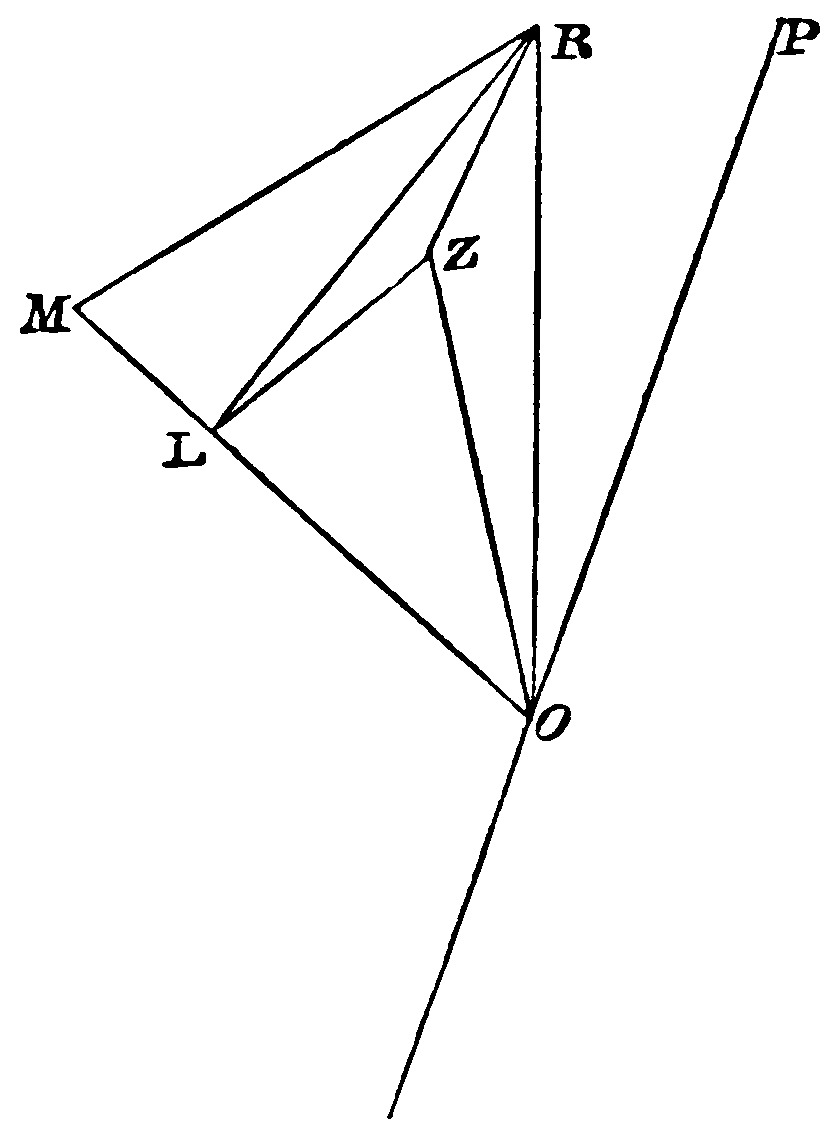
\includegraphics[width=0.4\textwidth]{018.png}
\centering
\end{figure}

\(MR=r\), \(RZ=r\cos\theta\), \(ML=r\sin\theta\cos\phi\), \(ZL=r\sin\theta\sin\phi\).

Now
\[OR^2 = OL^2 + RL^2 = (OM-r\sin\theta\cos\phi)^2 + RL^2;\]
that is
\[OR^2=OM^2 - 2OMr\sin\theta\cos\phi + r^2;\]
therefore
\[(1 + \alpha\mu')^2 = (1 + \alpha\mu)^2 - 2(1 + \alpha\mu) r\sin\theta\cos\phi + r^2.\]

Solve this quadratic in \(r\), and neglect powers of \(\alpha\) above the
first: thus
\[r = (1 + \alpha\mu)\sin\theta\cos\phi \pm\left\{(1 + \alpha\mu)\sin\theta\cos\phi + \frac{\alpha(\mu' - \mu)}{\sin\theta\cos\phi}\right\}.\]

The upper sign must be taken; for the lower sign would lead
to a value of \(r\) of the order \(\alpha\): therefore
\[r = 2(1 + \alpha\mu)\sin\theta\cos\phi + \frac{\alpha(\mu' -\mu)}{\sin\theta\cos\phi}.\]

\Section
768. The limits of the integrations, without introducing any
error of the order we are retaining, may be taken to be \(0\) and \(\pi\)
for \(\theta\), and \(- \xp\dfrac{\pi}{2}\) and \(\xp\dfrac{\pi}{2}\) for \(\phi\). Hence using the value of \(r\) found in
the preceding Article we have
%%-----File: 019.png-----%%
\[\begin{aligned}
A &= \frac{4\pi}{3} - \frac{2\pi\alpha\mu}{3} + \alpha\iint\mu' \sin\theta\, d\theta\, d\phi,\\
B &= \alpha\iint(\mu' - \mu) \frac{\sin\theta \sin\phi}{\cos\phi}\, d\theta\, d\phi,\\
C &= \alpha\iint(\mu' - \mu) \frac{\cos\theta}{\cos\phi}\, d\theta\, d\phi.
\end{aligned}\]

Here \(B\) is estimated \textit{towards} the pole; if we estimate \(B\) \textit{from} the
pole, as Laplace does, we must change the sign of the expression.

\Section
769. Laplace then incautiously says that
\[B = -\alpha\int\frac{ \mu' \sin\theta \sin\phi}{\cos\phi}\, d\theta\, d\phi,\qquad C = \alpha\int \frac{\mu' \cos\theta}{\cos\phi}\, d\theta\, d\phi;\]
but he never uses these erroneous forms, and probably the introduction
of them is only a misprint. These erroneous forms would
make \(B\) and \(C\) infinite.

\Section
770. In order to effect the integrations in the values of \(A\),
\(B\), and \(C\), supposing \(\mu'\) a known function of \(\psi'\) and \(\lambda'\), it would
be necessary to connect \(\psi'\) and \(\lambda'\) with \(\theta\) and \(\phi\): to this we
proceed.

It will be seen that \(\mu'\) enters with the coefficient \(\alpha\); and thus
we may use approximations in our equations.

In the diagram of Art.\ 767, by projecting on \(OP\) the straight
line \(OR\), and also the broken line made up of \(OL\) and \(LZ\), we
have exactly
\[\begin{aligned}
OR \cos\psi' &= OL \cos\psi + LZ \sin\psi\\
&= (OM - r \sin\theta \cos\phi) \cos\psi + r \sin\theta \sin\phi \sin\psi;
\end{aligned}\]
that is
\[OR \cos\psi' = OM \cos\psi - r \sin\theta \cos(\phi + \psi).\]

Hence to the order which we have to retain
\[\cos\psi' = \cos\psi - 2 \sin^2\theta \cos\phi \cos(\phi + \psi)\tag{1}.\]

Again,
\[\sin(\lambda' - \lambda) = \frac{RZ}{OR \sin\psi'} = \frac{r \cos\theta}{OR \sin\psi'}.\]

Hence to the order which we have to retain
\[\sin(\lambda' - \lambda) = \frac{2 \sin\theta \cos\theta \cos\phi}{\sin\psi'}\tag{2}.\]
%%-----File: 020.png-----%%

Equations (1) and (2) theoretically give us the required connection
of \(\psi'\) and \(\lambda'\) with \(\theta\) and \(\phi\).

\Section
771. Laplace proceeds to establish the following result:
\[
\frac{dA}{d\psi} = - \frac{2\pi\alpha}{3} \frac{d\mu}{d\psi} + \frac{B}{2}.
\]

This corresponds to equation (5) of Art.\ 755. There is a difference
in sign however, because Laplace here estimates \(B\) \textit{from}
the pole, whereas in his second memoir he estimated it \textit{towards}
the pole: we shall for convenience keep here to the method of the
third memoir.

Laplace arrives at his result by four pages of integration and
differentiation: we shall not reproduce this investigation, as
Laplace himself afterwards gave a simpler process, and we shall
have to return to the subject.

This is the second appearance in Laplace's writings of the
theorem to which we have referred in Art.\ 755: it is here extended
to the case of a body not of revolution.

\Section
772. In the same manner as the theorem in Art.\ 771 is
established, we may shew that
\[
\frac{dA}{\sin\psi \,d\lambda} = - \frac{2\pi\alpha}{3} \frac{d\mu}{\sin\psi \,d\lambda} + \frac{C}{2}.
\]

\Section
773. If we now consider the condition of relative equilibrium
of a fluid mass, or of a mass covered with a superficial stratum of
fluid, we arrive as in Art.\ 756 at the following results:
\[
\begin{aligned}
B &+ \omega^2 \sin\psi \cos\psi = \frac{4 \pi\alpha}{3} \frac{d\mu}{d\psi} ,\\
P &= P_0 - \frac{5}{4} \omega^2 \sin^2 \psi,
\end{aligned}
\]
where \(B\) is now estimated \textit{from} the pole.

And we have now besides
\[
C = \frac{4 \pi\alpha}{3 \sin\psi} \frac{d\mu}{d\lambda}\text{.}
\]

These general results must have been very interesting at the
time they were given: but they have since lost much of their
%%-----File: 021.png-----%%
value, because it is known that under the supposed conditions
the mass can only take the form of an oblatum: this was established
by Laplace in his fourth memoir, and the demonstration
is reproduced in the \textit{Mécanique Céleste}: see Livre \textsc{iii}.\ § 26.

\Section
774. Laplace extends his process; for he supposes that
besides the attraction of the mass itself there may be external
forces: and in particular he considers the case of an external body
which is in relative equilibrium with respect to the attracted
body. In this case we have as usual to find, not the absolute
attraction at a point, but the excess of this attraction above that
at the centre of gravity of the mass. Laplace's method is peculiar:
see his pages 87 and 88. The result is correct, but a reader
will probably verify it, as he easily may, before he accepts it.

\Section
775. On pages 261\dots 267 of the Paris \textit{Mémoires} for 1776, we
have an \textit{Addition} to the memoir we are now considering. This
Addition gives us a simple proof of the theorems of Arts.\ 771
and 772 in the more general form which they take when the
force of attraction is supposed to vary as the \textit{n}th power of the
distance. The investigation depends on the same principles as
that in the \textit{Mécanique Céleste}, Livre \textsc{iii}.\ § 10; and the results may
be said to be summed up in equation (1) of that section, inasmuch
as they will follow from that equation by differentiation. But the
Potential Function is not used in the pages now under notice.
These pages are in substance reproduced in the fourteenth section
of Laplace's \textit{Théorie \dots\ de la Figure des Planetes} of which we shall
hereafter give an account.

\Section
776. I will notice some remarks on page 262 by which
Laplace tries to shew that if there is one figure of equilibrium
for a rotating spheroid there will be an infinite number.

Let \(1 + \alpha y\) be the radius vector to any point of the surface,
where \(\alpha\) is indefinitely small (\textit{infiniment petit}), and \(y \) is any function
of \(\theta\) the colatitude and \(\varpi\) the longitude. Let \(\alpha B\) denote the
tangential attraction; then for equilibrium we must have \(B = 0\).
Let \(y\) be such a function of \(\theta\) and \(\varpi\) as to satisfy this: then he
says the condition will also be satisfied when we put \(\theta + a\) for \(\theta\),
%%-----File: 022.png-----%%
and \(\varpi + b\) for \(\varpi\); where \(a\) and \(b\) are constants. Let \(y'\) be what
\(y\) becomes by this change. Then he says that there will be equilibrium
if the radius vector be \(1 + \alpha y'\); and therefore also if the
radius vector be \(1 + \alpha y + n \alpha y'\) where \(n\) is any constant.

I presume that Laplace does not suppose any rotation here,
or any action but that of the fluid mass itself. Thus in fact we
have a case something like that of the coexistence of small motions
in Dynamics.

If we suppose the mass to rotate then the argument will have
to be slightly modified. We cannot then change \(\theta\) into \(\theta + a\),
but we can change \(\varpi\) into \(\varpi + b\); and thus as before we shall
still have an infinite number of solutions. Compare the \textit{Mécanique
Céleste}, Livre \textsc{iii}.\ § 26.

\Section
777. The first three memoirs by Laplace on our subjects are
superseded by his investigations of the third division: see Art.\ 741.
The first three memoirs may be considered to attach themselves
to the researches of D'Alembert, and to continue those researches.
In his writings of the third division Laplace may be said to derive
great assistance from Legendre. It will be necessary as we proceed
to be particular with the chronology of the memoirs by
Laplace and Legendre; for we shall find indications that Legendre
was not quite satisfied with Laplace's silence as to the matter of
priority: see also Pontécoulant's \textit{Système du Monde}, Vol.\ \textsc{iii}.\
page x.

\Section
778. The order then which we shall have to adopt after thus
considering Laplace's first three memoirs is the following:

Legendre's first memoir; this is in the \textit{Mémoires \dots\ par divers
Savans} \dots\ Vol.\ \textsc{x.}

Laplace's treatise \textit{De la Figure des Planetes}; this is contained
in a work published in 1784.

Legendre's second memoir; this is in the Paris \textit{Mémoires}
for 1784.

Laplace's fourth memoir; this is in the Paris \textit{Mémoires} for 1782.

Laplace's fifth memoir; this is in the Paris \textit{Mémoires} for 1783.
%%-----File: 023.png-----%%

Laplace's sixth memoir; this is in the Paris \textit{Mémoires} for 1787.

Legendre's third memoir; this is in the Paris \textit{Mémoires} for 1788.

Legendre's fourth memoir; this is in the Paris \textit{Mémoires} for 1789.

Laplace's seventh memoir; this is in the Paris \textit{Mémoires} for 1789.

When a volume of the Paris \textit{Mémoires} is said to be for a
specified year, it by no means follows that all the memoirs which
it contains were written during or before the specified year. The
order in which we have placed these writings of Laplace and
Legendre is the order of their production, as will appear by our
extracts from them as we proceed.
%%-----File: 024.png-----%%

\Chapter{CHAPTER XX.}
\Subhead{LEGENDRE'S FIRST MEMOIR.}
\Runhead{\textsc{legendre's first memoir.}}

\Section
779. \textsc{A very} important memoir by Legendre is contained
in the tenth volume of the \textit{Mémoires \dots\ présentés par divers
Savans\dots.} The date of publication of the volume is 1785. The
memoir, however, must have been communicated to the Academy
at an earlier period; for in the treatise \textit{De la Figure des Planetes},
which was published in 1784, Laplace refers to the researches of
Legendre which constitute the present memoir: see page 96 of
Laplace's treatise.

Legendre's memoir is entitled \textit{Recherches sur l'attraction des
sphéroïdes homogènes}; it occupies pages 411\dots 434 of the volume.

\Section
780. Legendre begins thus:
\begin{squote}
M. Maclaurin est le premier qui ait déterminé l'attraction d'un
Sphéroïde elliptique pour les points situés dans son intérieur ou à sa
surface. Les propositions qu'il a établies à ce sujet, et d'où résulte une
solution si simple du problême de la figure de la Terre, servent de base
à son excellente Pièce sur le Flux et le Reflux de la Mer, et sont
connues de tous les Géomètres. Le même Auteur a considéré aussi
l'attraction des Sphéroïdes elliptiques sur les points situés au dehors;
mais il s'est borné aux points situés sur l'axe ou sur l'équateur pour les
Sphéroïdes de révolution, et seulement aux points placés dans la direction
d'un des trois axes, lorsque le Sphéroïde a toutes ses coupes elliptiques.
Ces deux objets se trouvent compris dans un théorème remarquable,
dont M. Maclaurin donne l'énoncé, art.\ 653 de son Traité
des Fluxions; théorême dont MM. d'Alembert et de la Grange ont
donné depuis la démonstration; le premier, dans les Mémoires de
Berlin, année 1774, et dans le tome \textsc{vii}.\ de ses Opuscules; le second,
dans les Mémoires de Berlin, année 1775.
%%-----File: 025.png-----%%

Il ne paroît pas que les Géomètres aient poussé plus loin leurs
recherches sur cette matière intéressante; car, quoique M. de la Grange
ait considéré le problême dans toute sa généralité (Mém.\ de Berlin,
année 1773), l'intégration n'a réussi à ce grand Géomètre que dans les
cas déjà résolus par M. Maclaurin. C'est dans la vûe de concourir
à la perfection de cette théorie, que j'ai entrepris les Recherches dont
je vais rendre compte.
\end{squote}

We see from this extract that, as we have stated in Art.\ 260,
Legendre underrates what Maclaurin really did demonstrate.

\Section
781. We will now give in substance Legendre's treatment
of Maclaurin's theorem in attractions.

Let the equation to an ellipsoid be \(\xp\dfrac{x^2}{a^2} + \xp\dfrac{y^2}{b^2} + \xp\dfrac{z^2}{c^2} = 1\): required
the attraction at a point on the prolongation of the axis of \(x\) at the
distance \(h\) from the origin.

Let \(r\) be the distance of any point of the ellipsoid from the
attracted particle, \(\phi\) the angle between \(r\) and its projection on the
plane of \((x, z)\), and \(\psi\) the angle between this projection and the
axis of \(x\). The element of mass is \(r^2 \cos \phi d\phi d\psi dr\); and thus the
attraction resolved along the axis on which the attracted particle
is situated is
\[\frac{r^2 \cos \phi d\phi d\psi dr}{r^2} \times \cos\phi \cos\psi,\]
that is
\[\cos^2 \phi \cos \psi d\phi d\psi dr.\]
We first integrate for \(r\); the limits are \(r_1\) and \(r_2\), where \(r_1\) and \(r_2\)
are the limiting radii vectores drawn from the attracted particle
to the ellipsoid in the direction assigned by the angles \(\phi\) and \(\psi\).
Thus \(r_1\) and \(r_2\) are the roots of the quadratic equation
\[\frac{(h - r \cos\phi \cos\psi)^2}{a^2} + \frac{r^2 \sin^2\phi}{b^2} + \frac{r^2 \cos^2 \phi \sin^2 \psi}{c^2} = 1;\]
hence we find that
\begin{multline*}
r_2 - r_1 =\\
\frac{2abc\xsurd \{c^2 (a^2 - h^2) \sin^2 \phi + b^2 \cos^2 \phi (a^2 \sin^2 \psi + c^2 \cos^2 \psi - h^2 \sin^2 \psi)\}}{b^2c^2 \cos^2 \phi \cos^2 \psi + a^2c^2 \sin^2 \phi + a^2b^2 \cos^2 \phi \sin^2 \psi}.
\end{multline*}
%%-----File: 026.png-----%%

Now \((r_2 - r_1)\cos^2 \phi\cos \psi\) can be integrated with respect to \(\psi\);
for we may put the expression to be integrated in the form
\[
\frac{Kd\psi\cos \psi \xsurd(A^2 - B^2\sin^2 \psi)}{1 + L\sin^2 \psi}
\]
where \(A\), \(B\), \(K\), and \(L\) do not involve \(\psi\).

The integral with respect to \(\psi\) is to be taken between such
limits as make \(r_2 - r_1\) vanish, that is between the limits given by
\[
\sin \psi = \pm \frac{A}{B}.
\]

Assume \(\sin \psi = \xp\dfrac{A}{B}\sin \zeta\); thus the integral becomes
\[
\frac{KA^2}{B} \frac{\cos^2 \zeta d\zeta}{1 + \dfrac{LA^2}{B^2} \sin^2 \zeta}\text{.}
\]

The limits for \(\zeta\) are \(- \xp\dfrac{\pi}{2}\) and \(\xp\dfrac{\pi}{2}\). This gives for the value of
the integral
\[
\frac{\pi KB}{L} \left\{\sqrt{\vphantom{\frac{A}{B}}}\left(1 + \frac{LA^2}{B^2}\right) - 1\right\}.
\]

Substitute for \(A\), \(B\), \(K\), and \(L\); and then the required attraction
becomes
\[
\frac{2\pi ach}{a^2 - c^2} \int \left\{ \sqrt{\vphantom{\frac{a}{b}}}
\left( \frac{c^2\sin^2 \phi + b^2\cos^2 \phi}{a^2\sin^2 \phi + b^2\cos^2 \phi} \right)
- \frac{\xsurd (h^2 - a^2 + c^2)}{h} \right\} \cos \phi d \phi\text{.}
\]

The limits of \(\phi\) are such as make \(r_2 - r_1\) vanish when \(\psi = 0\);
hence they are obtained by putting \(A = 0\): we shall find that this
gives
\[
\sin \phi = \pm\frac{b}{\xsurd(h^2 - a^2 + b^2)}\text{.}
\]

Assume \(\sin \phi = \dfrac{b\sin \theta}{\xsurd(h^2 - a^2 + b^2)}\); then the limits of \(\theta\) will be \(- \dfrac{\pi}{2}\)
and \(\dfrac{\pi}{2}\). Put \(M\) for \(\xp\dfrac{4abc}{3}\), that is the volume of the ellipsoid. Hence
finally the attraction is equal to
%%-----File: 027.png-----%%
\begin{multline*}
\frac{3Mh}{(a^2 - c^2) \xsurd(h^2 - a^2 + b^2)} \int_0^{\tfrac{\pi}{2}} \left\{\sqrt{\vphantom{\frac{a}{b}}} \left(\frac{ h^2 - a^2 + b^2 + (c^2 - b^2) \sin^2 \theta}{ h^2 - a^2 + b^2 + (a^2 - b^2) \sin^2 \theta} \right)\right.\\
- \left.\frac{\xsurd (h^2 - a^2 + c^2)}{h}\right\} \cos \theta\, d \theta.
\end{multline*}

Now for confocal ellipsoids \(a^2 - b^2\), \(a^2 - c^2\), and \(b^2 - c^2\) are constant;
hence for such ellipsoids the attraction at the assigned
point varies as the mass of the ellipsoid.

\Section
782. Legendre expresses his belief that the theorem of
Maclaurin respecting the attraction of confocal ellipsoids holds
whatever be the position of the attracted particle; see his page 413.
This we now know is true, for it was demonstrated by Laplace.
But Legendre was at this time unable to give a complete demonstration;
and so confined himself to the case of ellipsoids of
revolution.

In order to prepare the way for this demonstration he first
establishes a very remarkable theorem, namely: \textit{if the attraction
of a solid of revolution is known for every external point which is
on the prolongation of the axis it is known for every external point.}

\Section
783. Legendre's demonstration of the important result just
stated is conducted by the aid of series. We here for the first
time meet those famous coefficients which it is usual to call
\textit{Laplace's coefficients}; and we see that to Legendre really belongs
the honour of introducing them.

These functions might with propriety be called Legendre's
functions when they involve only one variable, and Laplace's functions
when they involve two: Legendre himself seems to acquiesce
in this in a passage at the beginning of his fourth memoir. But
in consideration of the great use which Laplace has made of these
coefficients, and of the important extension which he has given to
the theory of them, I shall continue to use the common English
title of Laplace's coefficients for them, after having formally recognised
the rights of Legendre.

We may observe that Legendre's researches with respect to
Laplace's coefficients are reproduced with extended generality in
his \textit{Exercices de Calcul Intégral}, Vol.\ \textsc{ii}.\ 1817, pages 247\dots 273.
%%-----File: 028.png-----%%

\Section
784. An important work on the branch of analysis of which
Laplace's coefficients is the origin is Heine's \textit{Handbuch der Kugelfunctionen},
published at Berlin in 1861: to this I shall occasionally
refer. The preface to Heine's work gives the evidence for the
priority of Legendre to Laplace in the introduction of these coefficients;
and also for the recognition of this fact by Jacobi and
Dirichlet.

\Section
785. The following is the definition of Laplace's coefficients:
Let \((1 - 2\alpha \cos\psi + \alpha^2)^{- \frac{1}{2}}\) be expanded in ascending powers of \(\alpha\);
and let \(P_n\alpha^n\) denote the general term: then \(P_n\) is a function of
\(\cos\psi\), and is called Laplace's coefficient of the \(n\)th order.

\Section
786. In the present memoir Legendre has occasion to use
only the coefficients of an \textit{even} order, because he supposes that
his attracting body is symmetrical with respect to the equator.
He writes down the values of \(P_2\), \(P_4\), \(P_6\), and \(P_8\); and from these
the general form of the coefficient for an even order may be easily
perceived. We have, as shewn by Heine in his page 6:
\begin{multline*}
P_n = \frac{1 \ldot 3 \ldot 5 \ldots (2n - 1)}{\oldfactorial{n}} \left\{ x^n - \frac{n(n-1)}{2(2n-1)} x^{n-2}\right.\\
+\left.\frac{n(n-1)(n-2)(n-3)}{2 \ldot4 \ldot (2n-1)(2n-3)} x^{n-4} - \ldots \right\},
\end{multline*}
where \(x = \cos\psi\). Legendre's values are particular cases of this
general expression.

This general expression may be easily obtained by first expanding
\((1 - 2\alpha x + \alpha^2)^{-\frac{ 1}{2}}\) in the form
\[1 + \frac{1}{2} \alpha (2x - \alpha) + \frac{1 \ldot 3}{2\ldot 4} \alpha^2 (2x-\alpha)^2 + \frac{1 \ldot 3 \ldot 5}{2 \ldot 4 \ldot 6} \alpha^3 (2x-\alpha)^3 + \ldots,\]
and then selecting the term in \(\alpha^n\) from each of these.

\Section
787. Legendre arrives at an important property of Laplace's
coefficients. Suppose that for \(\alpha\) or \(\cos\psi\) we write
\[\cos\theta \cos\theta' + \sin\theta \sin\theta' \cos\omega,\]
then \(P_n\) becomes a function of \(\theta\), \(\theta'\), and \(\omega\); integrate with respect
to \(\omega\) from \(0\) to \(2\pi\); then the result is a function of \(\theta\) and \(\theta'\). This
%%-----File: 029.png-----%%
result will be of the form \(2\pi f(\cos \theta)f(\cos \theta')\); that is it will be
the product of a certain function of \(\cos \theta\) into the same function
of \(\cos \theta'\); and \(f(\cos \theta)\) is in fact \(P_n\), when \(x\) is put for \(\cos \theta\).
Legendre demonstrates this for the case which he requires, that is
for the case of a coefficient of an \textit{even} order; and he obtains the
correct form for the function which we denote by \(f\). Legendre's
demonstration shews his energy and perseverance, but to a modern
student it will appear laborious and uninviting.

The property here considered follows immediately from the
general expressions which have been since given for Laplace's
coefficients when treated as functions of \(\theta, \theta'\), and \(\omega\), in the manner
above indicated. See the \textit{Mécanique Céleste}, Livre \textsc{iii}.\ § 15.

\Section
788. Another important theorem respecting the coefficients
is briefly indicated by Legendre on his page 426: it is demonstrated
in Legendre's second memoir, being the last of the seven
theorems which are there investigated: see Art.\ 830.

\Section
789. In this memoir we meet for the first time the function
\(V\) which we now call the \textit{Potential}, and which denotes the sum
of the elements of a body divided by their distances from a fixed
point. The introduction of this function Legendre expressly
assigns to Laplace. The following are the circumstances.

A point is situated outside a solid of revolution. Legendre
has to determine the attractions of the solid at the point, along
the radius vector which joins the point to the centre of the solid,
and at right angles to this direction. He has found a series for
the former; and he says the latter might be determined by similar
investigations; then he adds:
\begin{squote}
\dots\ mais on y parvient bien plus facilement à l'aide d'un Théorême
que M. de la Place a bien voulu me communiquer: voici en quoi il
consiste.
\end{squote}

Then follows the theorem which is enunciated and immediately
demonstrated. The theorem is that the attraction along
the radius vector is \(-\xp\dfrac {dV}{dr}\), and the attraction at right angles to
the radius vector is \(- \xp\dfrac{dV}{rd\theta}\); where \(r\) is the radius vector, and \(\theta\)
%%-----File: 030.png-----%%
the angle which it makes with the axis of the solid: these attractions
being estimated towards the centre, and the pole respectively.

These statements relative to the function \(V\) are now well
known and given in elementary books.

\Section
790. We may observe that the name \textit{Potential} was first used
by the late George Green, in his \textit{Essay on the Application of
Mathematical Analysis to the Theories of Electricity and Magnetism},
published in 1828: see his page 9, or page 22 of the
volume in which Green's works were collected and reprinted
in 1871. Gauss used the word in his memoir entitled \textit{Allgemeine
Lehrsätze in Beziehung auf die \dots\ Anziehungs-und-Abstossungs-Kräfte},
published in 1840. As Gauss does not refer to any
previous authority we are, I presume, to infer that he had independently
selected the name.

\Section
791. Let us briefly indicate the demonstration of Legendre's
remarkable theorem enunciated in Art.\ 782. We shall use the
\textit{potential} throughout, whereas Legendre himself only used it
partially. But substantially the demonstration we shall give
is Legendre's.

Let \(r\) and \(\theta\), as in Art.\ 789, be the polar coordinates of the
attracted particle; let \(r'\) and \(\theta'\) be the corresponding two polar
coordinates of an element of the attracting body; let \(\omega\) be the
difference of longitude, as we may call it, of the attracted point
and the attracting element. Then, taking the density as unity,
the element of the attracting mass is \(r'^2 \sin\theta'\, d\theta'\, d\omega\, dr'\). Thus
\[V =\iiint \frac{r'^2 \sin \theta'\, d\theta'\, d\omega\, dr'}{\xsurd(r'^2 - 2rr' \cos \psi + r^2)},\]
where
\[\cos \psi = \cos \theta \cos \theta' + \sin \theta \sin \theta' \sin \omega.\]

Expanding the denominator in ascending powers of \(\dfrac{r'}{r}\) we have
\[V = \iiint \frac{r'^2}{r}\left\{1+P_1 \frac{r'}{r} + P_2 \frac{r'^2}{r^2} + P_3\frac{r'^3}{r^3} + \ldots\right\} \sin \theta'\, d\theta' \,d\omega\, dr'.\]

We integrate first with respect to \(r'\); and, since the attracting
body is assumed to be symmetrical with respect to its equator,
%%-----File: 031.png-----%%
the limits will be \(-s\) and \(s\), where \(s\) is the radius vector of the
solid corresponding to a colatitude \(\theta'\). Thus
\[V = 2 \iint\frac{ s^3}{r} \left\{\frac{1}{3} + \frac{P_{2}}{5} \frac{s^2}{r^2} + \frac{P_{4}}{7} \frac{s^4}{r^4} + \ldots\right\} \sin \theta'\, d\theta' d\omega.\]

Now we integrate with respect to \(\omega\) between the limits \(0\) and
\(2\pi\). Then by the theorem of Art.\ 787, we obtain for \(V\) a series
of which the first term is \(\xp\dfrac{\text{Mass}}{r}\); and for the following terms
the general form is
\[\frac{4\pi f_{2n} (\cos \theta)}{(2n + 3) r^{2n+1}} \int f_{2n} (\cos \theta') s^{2n+3} \sin \theta'\, d\theta'.\]

The limits for \(\theta'\) are \(0\) and \(\xp\dfrac{\pi}{2}\). The integration could not be
effected until the form of the attracting body is assigned so as to
make \(s\) a known function of \(\theta'\). We shall denote the integral
by \(L_{2n}\); it will be some numerical quantity. Thus the general
term of \(V\) is
\[\frac{4\pi f_{2n}(\cos \theta)L_{2n}}{(2n + 3)r^{2n+1}}.\]

Here \(f_{2n} (\cos\ \theta)\) is a certain known function of \(\cos \theta\) which is
independent of the form of the body; moreover this function does
not vanish when \(\theta=0\). Now if the attraction is known at all
points which are on the prolongation of the axis, it follows that
\(V\) must also be known for all such points. Hence all the quantities
of which \(L_{2n}\) is the type must be known. Therefore \(V\) is
known for all external points; and therefore the attraction is also
known for all external points.

The demonstration is in substance reproduced by Laplace in
the \textit{Mécanique Celeste}, Livre \textsc{iii}.\ § 17.

\Section
792. It must be observed that the preceding demonstration
is satisfactory only so long as \(r\) is greater than the greatest radius
vector of the body, so that we may be sure of having convergent
series throughout. The subject is discussed by Poisson in the
\textit{Connaissance des Tems} for 1829; he shews that the formulæ
used by Legendre and Laplace are correct, to the third order of
the standard small quantity inclusive. I have extended Poisson's
investigation in a paper published in the \textit{Proceedings of the Royal
Society}, Vol.\ \textsc{xx}.
%%-----File: 032.png-----%%

\Section
793. We can now demonstrate Legendre's extension of
Maclaurin's theorem respecting the attraction of an ellipsoid of
revolution.

Put \(b = c\) in the result of Art.\ 781; then it becomes
\[
\frac{3M}{a^2 - b^2} \int \left\{ \frac{h}{\xsurd \{h^2 - a^2 + b^2 - (b^2 - a^2)\sin^2 \theta\}}
- 1 \right\}\cos \theta \, d\theta;
\]
and \(\{h^2 - a^2 + b^2 - (b^2 - a^2)\sin^2 \theta\}^{-\frac{1}{2}}\) can be expanded by the Binomial
Theorem in a convergent series of powers of
\[
\frac{(b^2 - a^2)\sin^2 \theta}{h^2 - a^2 + b^2},
\]
so that the attraction can be expressed in a convergent series
which is a function of \(a^2 - b^2\), and thus remains the same for confocal
ellipsoids of revolution.

Thus for points on the prolongation of the axis of revolution
the attractions of confocal ellipsoids at the same point are as the
masses of the ellipsoids. Then by the aid of Art.\ 791 it follows
that this will hold for \textit{any} external point.

Legendre himself integrates before expansion; this does not
affect the essence of his method. The integral takes different
forms according as \(a\) is greater or less than \(b\).

\Section
794. In conclusion we may affirm that no single memoir in
the history of our subject can rival this in interest and importance.
During forty years the resources of analysis, even in the hands
of D'Alembert, Lagrange, and Laplace, had not carried the theory
of the attraction of ellipsoids beyond the point which the geometry
of Maclaurin had reached. Legendre now extended the
chief result of that geometry, by shewing that it was true in the
case of an ellipsoid of revolution for any external point. The
introduction of the coefficients now called Laplace's, and their
application to the remarkable theorem of Art.\ 782, commence a
new era in mathematical physics. Moreover the existence and
the value of the potential function were now first manifested.

It is not too much to say that this memoir is the foundation
for all that Laplace added in the theories of Attraction and the
Figure of the Earth to the works of Maclaurin and Clairaut.
%%-----File: 033.png-----%%

\Chapter{CHAPTER XXI.}
\Subhead{LAPLACE'S TREATISE.}
\Runhead{\textsc{laplace's treatise.}}

\Section
795. \textsc{We} are now about to notice a work by Laplace entitled
\textit{Théorie du Mouvement et de la Figure Elliptique des Planetes}; this
is a quarto volume which was published in 1784. The title-page
and preface occupy xxiv pages; then the first part, which is on
the theory of the elliptic motion of the planets, occupies pages 1\dots 66;
the second part, which is on the figure of the planets, extends from
page 67 to page 150: an addition to the first part is given on
pages 150\dots 152, and a list of errata on page 153.

\Section
796. The volume is scarce, and seems but little known. The
late Professor De Morgan in a note to his article \textit{Table} in the
\textit{English Cyclopædia} remarked:
\begin{squote}
When a person is distinguished by one particular work, his other, and
particularly his previous, writings, even on the same subject, go out of
notice. How many persons, for instance, know that Laplace published
(separately from the Memoirs of the Academy) a small work on the
elliptic motion and on the figures of the planets, in 1784? (See Lalande,
Bibl.\ Astron.\ ann.\ 1784.) And how many biographical accounts of
Laplace mention it?
\end{squote}

My copy of this work formerly belonged to Mechain, and
subsequently to Arago. There are some irregularities in the
paging: no pages occur numbered 105, 106, 145, 146; on the
other hand, pages numbered 129, 130 occur twice.

According to a bookseller's catalogue, a German translation of
the work by J. J. A. Ide was published at Berlin in 1800; but I
have not seen it.
%%-----File: 034.png-----%%

\Section
797. The circumstances which led to the publication of the
work are thus stated by Laplace in the preface, pages xviii and xix:
\begin{squote}
Une des propriétés les plus remarquables de la loi de pesanteur qui a
lieu dans la Nature, est de terminer les orbites des corps célestes par des
lignes du second ordre, et leurs figures par des surfaces du second ordre,
du moins lorsqu'on fait abstraction des petites inégalités qui troublent
leurs mouvemens et leurs figures. Cette propriété m'a fait naître depuis
long-tems l'idée d'exposer dans un ouvrage particulier, les principaux
résultats du mouvement et de la figure elliptiques des Planètes; mais
entraîné par d'autres occupations, j'aurois entiérement renoncé à ce
travail, sans le désir qu'un Magistrat également distingué par son rang,
par sa naissance, et par ses lumieres, m'a témoigné plusieurs fois, de voir
les propriétés des mouvemens elliptiques et paraboliques, déduites de la
seule considération des équations différentielles du second ordre qui
déterminent à chaque instant, le mouvement des corps célestes autour
du Soleil.
\end{squote}

In a note at the foot of the page the name of the distinguished
magistrate is given: M. de Saron, President du Parlement, Honoraire
de l'Académie Royale des Sciences.

The passage is very interesting as recording thus early a
design which was afterwards carried out on a larger scale by the
publication of the \textit{Mécanique Céleste}.

\Section
798. In a manuscript note in my copy it is stated that
M. Bochart printed the work at his own expense; I presume that
this is another name for M. de Saron.

Poisson has recorded the fact that an ellipsoid of revolution,
used by Coulomb in his experiments on electricity, was turned by
M. de Saron. \textit{Mémoires de l'Institut}, Vol.\ \textsc{xiii}.\ 1835, page 501.

\Section
799. The work which we are now about to examine may be
said to form the transition between Laplace's first three memoirs
which do not reappear in the \textit{Mécanique Céleste}, and the subsequent
memoirs which do. In the present work Laplace introduces
what we call the \textit{potential}, but not what we call \textit{Laplace's functions};
although these functions had already been used by Legendre:
see Art.\ 783.
%%-----File: 035.png-----%%

\Section
800. The treatise \textit{De la Figure des Planetes} is arranged in
seventeen sections; the first seven sections relate to attractions,
the next six to the relative equilibrium of a mass of rotating fluid,
and the rest principally to the value of gravity at the surface of
such a body.

\Section
801. The first section, on pages 67 and 68, is preliminary.
The equation to an ellipsoid is given under the form
\[x^2 + my^2 + nz^2 = k^2.\]
This notation appears repulsive to modern readers, trained to
study symmetry; but it has been adopted by very eminent mathematicians.
Lagrange in his memoir of 1773, and Poisson in his
memoir of 1835, also employ \(m\), \(n\), \(k\) in the sense here adopted.

\Section
802. The second section, on pages 69\dots 73, defines the potential
function \(V\), and expresses by means of it the attraction
of a body on a particle resolved parallel to three coordinate axes.
As we have already seen in Art.\ 789, the function was introduced
by Laplace into mathematical science.

\Section
803. In the third section, on pages 73\dots 78, polar coordinates
are employed. It is shewn that \(V\) may be expanded into an
infinite series; and in particular some of the properties of this
series, in the case of an ellipsoid, are noticed.

\Section
804. The fourth section, on pages 78\dots 86, is very important.
Laplace forms three equations involving \(V\), and the differential
coefficients of \(V\) taken with respect to \(m\), \(n\), \(k\), and the coordinates
\(a\), \(b\), \(c\) of the attracted particle. Then from these Laplace obtains
a demonstration of the theorem which I call by his name, being
the extension of Maclaurin's: see Art.\ 254. This is the first appearance
of the demonstration in print; but we learn from
page 97 of the treatise we are considering that the demonstration
was communicated to the Academy in May, 1783: see Art.\ 806.

The demonstration is given in an improved form in Laplace's
fourth memoir; and in this improved form it is reproduced in
the \textit{Mécanique Céleste}, Livre \textsc{iii}.\ § 5 and § 6: we shall defer our
remarks on it until we treat of the \textit{Mécanique Céleste}.
%%-----File: 036.png-----%%

The operations of the fourth section of Laplace's treatise are
somewhat developed in a memoir by Plana in the \textit{Memorie \dots\ Societa
Italiana}, Vol.\ \textsc{xv}.\ Modena, 1811.

\Section
805. The fifth section, on pages 86\dots 90, treats of the attraction
of an ellipsoid on an internal particle. The attraction parallel
to an axis of the ellipsoid is reduced to a single definite integral;
thus Laplace values and appropriates the treasure which
D'Alembert deliberately threw away: see Art.\ 651. This section
is embodied in the \textit{Mécanique Céleste}, Livre \textsc{iii}.\ § 3.

We know that the integral can be expressed by means of
elliptic functions; Laplace had convinced himself that it could
not be expressed by the ordinary functions, but he did not publish
his argument. After shewing that the integral, although \textit{definite},
involved all the difficulty of the \textit{indefinite} integral, he says on
his page 90:
\begin{squote}
L'intégrale indéfinie des fonctions différentielles de la forme
\(\xp\dfrac{x^2\, dx}{\sqrt{(1+\alpha x^2)(1+\beta x^2)}}\), est impossible, excepté dans les deux cas suivants,
sçavoir lorsque l'une ou l'autre des quantités \(\alpha\), et \(\beta\), est nulle, ou
lorsqu'elles sont égales; je me suis assuré que dans tous les autres cas,
l'intégrale ne peut pas être exprimée par une fonction finie de quantités
algébriques, d'arcs de cercle et de logarithmes; ainsi l'expression intégrale
que nous venons de trouver \dots, est la plus simple que l'on puisse donner
à cette valeur, et il seroit inutile de chercher à la réduire en termes finis.
\end{squote}

In his fifth section Laplace demonstrates what he calls a remarkable
result, namely: that a particle placed within an elliptic
shell of any thickness, and of which the outer and inner surfaces
are perfectly similar, will be in equilibrium. This is apparently
the first formal statement of the result; but, as we have seen in
Art.\ 662, Frisi may be considered to have obtained it.

\Section
806. The sixth section, on pages 90\dots 97, continues the subject
of the attraction of an ellipsoid on an internal particle; and
it effects the integrations in the particular case of an oblatum.
This is embodied in the \textit{Mécanique Céleste}, Livre \textsc{iii}.\ § 7.

The section concludes with a sketch of the history of the
problem of the attraction of an ellipsoid. The mistake is made
%%-----File: 037.png-----%%
with respect to Maclaurin which I have pointed out in Art.\ 260.
Laplace next speaks of the very ingenious method by which
Legendre had shewn that the theorem given by Maclaurin for the
case of a point on the prolongation of the axis was true for any
position of the point with respect to ellipsoids of revolution:
see Art.\ 793. Then Laplace concludes thus:
\begin{squote}
\dots\ mais la méthode de M. le Gendre, fondée sur la considération des
suites, n'est pas applicable aux ellipsoïdes qui ne sont point de révolution;
il étoit cependant très-vraisemblable que relativement à ces sphéroïdes,
le théorême de M. Maclaurin s'étendoit encore à un point situé d'une
maniere quelconque au-dehors; mais l'impossibilité d'intégrer les attractions
différentielles, du moins sous la forme que leur donnent les méthodes
connues, rendoit assez difficile la démonstration de ce théorême:
après quelques tentatives inutiles, j'y suis enfin parvenu par la méthode
précédente dont j'ai fait part à l'Académie au mois de Mai 1783. En
cherchant à transformer les attractions différentielles, on parviendroit,
selon toute apparence, à les rendre intégrables, par un choix convenable
des coordonnées; mais la méthode que j'ai suivie, m'ayant conduit
assez simplement au résultat que je cherchois, je n'ai point tenté d'autres
moyens, et j'ai pensé que le nouvel usage qu'elle présente, du calcul aux
différences partielles, pourroit être utile dans d'autres circonstances, et
par cette raison intéresser les Géomètres.
\end{squote}

I do not understand what is meant by the confident expectation
that the expression for the attraction could be integrated by
a suitable transformation: this seems to contradict the statement
made by Laplace in his fifth section: see Art.\ 805.

\Section
807. We now pass to the relative equilibrium of a rotating
fluid mass. The seventh section, on pages 97\dots 103, contains the
general equations of fluid equilibrium. This section is embodied
in the \textit{Mécanique Céleste}, Livre \textsc{i}.\ § 17 and § 34.

The section is followed by a \textit{Remarque} which criticises some of
Newton's investigations. I do not understand this criticism;
Laplace seems to assert that there is some fatal error of principle
which attaches to Newton's investigations on the Figure of
the Earth, the Tides, and Precession and Nutation: but in the
fifth volume of the \textit{Mécanique Céleste} it is stated on the other hand
%%-----File: 038.png-----%%
that Newton laid the true foundations of the theories of all these
subjects.

Laplace's words in the present Treatise are:
\begin{squote}
Newton, dans sa théorie de la figure de la terre, suppose cette planete
homogène et fluide à sa surface; il détermine dans cette hypothèse,
l'applatissement qu'elle doit avoir pour être en équilibre en vertu de son
mouvement de rotation, et de l'attraction de toutes ses parties.

Dans sa théorie du flux et du reflux de la mer, il cherche la figure
que cette masse doit prendre pour être en équilibre en vertu de son
mouvement de rotation, des attractions de toutes ses parties, et de celles
du Soleil et de la Lune.

Ce grand Géomètre ne s'est pas apperçu que si les choses se passoient
ainsi dans la nature, il ne pourroit y avoir, en vertu des attractions du
Soleil et de la Lune, aucune tendance au mouvement dans l'axe de rotation
de la terre, et qu'ainsi il n'y auroit ni précession des équinoxes, ni
nutation dans l'axe terrestre.
\end{squote}

\Section
808. The eighth section, on pages 103\dots 113, treats of the
relative equilibrium of a homogeneous mass of rotating fluid, acted
on by distant bodies as well as by its own attraction. The problem
is that which we have noticed in Art.\ 629. In the \textit{Mécanique
Céleste}, Livre \textsc{iii}.\ § 23, the action of the distant bodies is treated
in a simpler mode than in the present section. At the end of
Art.\ 629, I have drawn attention to two circumstances which it
seems to me that D'Alembert ought to have noticed; Laplace
says nothing about the first, but he alludes to the second, though
in scarcely an adequate manner. The present section contains an
important remark, to which I have already referred in Art.\ 153.

\Section
809. The ninth section, on pages 113\dots 116, applies the preceding
section to the case of the Moon supposed fluid and homogeneous.
Laplace arrives at the conclusion that the elongation of
the Moon's diameter directed towards the Earth is four times as
great as the elongation of the diameter which is at right angles to
this and in the plane of the Moon's orbit. We will briefly indicate
the process by which this is obtained. We have shewn in Art.\ 623,
what Laplace assumes at the outset, namely that the axis of rotation
will coincide with one of the principal axes of the Moon, and
the radius vector to the Earth with another.
%%-----File: 039.png-----%%

Take then \(\cos\lambda = 0\), \(\cos\mu = 0\), \(n = 0\), \(m = 0\); thus the axis of \(z\)
is that of rotation, and the axis of \(x\) passes through the Earth, the
centre of the Moon being the origin.

Then the last two equations of Art.\ 617 reduce to
\[a^2 \left(A - \frac{2M}{R^3} - \omega^2\right) = b^2 \left(B + \frac{M}{R^3} - \omega^2\right) = c^2 \left(C + \frac{M}{R^3}\right).\]

In Art.\ 616, we have spoken of a part of the action of \(M\) which
is not what we call a \textit{disturbing force}; in the present problem this
part is duly regarded, and is in fact balanced by what in common
language is called the centrifugal force arising from the revolution
of the Moon round the Earth. Moreover this revolution gives rise
to the following relation connecting the quantities involved:
\[\frac{M}{R^2} = R\omega^2.\]

Thus the above equations become
\[a^2 \left(A - \frac{3M}{R^3}\right) = b^2B = c^2\left(C + \frac{M}{R^3}\right).\]

We now require the values of \(A\), \(B\), and \(C\).

Put \(e^2\) for \(\xp\dfrac{a^2-b^2}{a^2}\) and \(e'^2\) for \(\xp\dfrac{a^2-c^2}{a^2}\); then \(e^2\) and \(e'^2\) being supposed
small we have approximately by Art.\ 620,
\[A= \frac{V}{a^3}\left\{1 + \frac{3}{10}(e^2 + e'^2)\right\}.\]

In like manner we can express \(B\) and \(C\); supposing that \(e^2\) and
\(e'^2\) will not be sensibly changed if we take \(b^2\) or \(c^2\) for denominator
instead of \(a^2\), we have
\[B=\frac{ V}{b^3} \left\{1 + \frac{3}{10} (e'^2 - 2e^2)\right\},\]
\[C=\frac{ V}{c^3} \left\{1 + \frac{3}{10} (e^2 - 2e'^2)\right\}.\]

Hence we shall obtain finally
\[e^2 = \frac{15}{2} \varpi,\qquad e'^2= 10\varpi,\]
%%-----File: 040.png-----%%
where \(\varpi\) stands for \(\xp\dfrac{M}{V}\ldot\xp\dfrac{a^3}{R^3}\), it being assumed that \(\varpi\) remains sensibly
unchanged if we multiply it by \(\xp\dfrac{c^2}{a^2}\).

Thus \(e'^2 - e^2 = \xp\dfrac{5}{2} \varpi\), so that \(e'^2 = 4(e'^2 - e^2)\); and this amounts
to Laplace's statement that one elongation is four times the other.

Laplace supposes that \(\xp\dfrac{M}{V} = \xp\dfrac{1}{70}\), and that \(\xp\dfrac{a}{R} = \sin 15'\, 45''\); and
thus he finds that \(a = \xp\dfrac{29712}{29711} c\), and \(b = \xp\dfrac{118845}{118844} c\).

\Section
810. The tenth section, on pages 116\dots 122, is devoted to the
case of a homogeneous fluid mass rotating with uniform angular
velocity, and acted on by its own attraction. Laplace says: ``Il est
visible qu'alors, le sphéroïde sera un ellipsoïde de révolution\dots.''
This is however more than he demonstrates, for he confines himself
to demonstrating that the oblatum is \textit{a} possible form of relative
equilibrium: see Art.\ 168. Laplace obtains the equation
which connects the angular velocity with the ellipticity of the
generating ellipse: see Art.\ 262. Laplace's investigations are
embodied in the \textit{Mécanique Céleste}, Livre \textsc{iii}., Chapitre \textsc{iii}. On his
page 121 Laplace says that we may presume the Earth to be
homogeneous from the centre up to a few leagues from the surface;
at a subsequent period he leaned to the opinion that the
density increases as we approach the centre; see the \textit{Mécanique
Céleste}, Livre \textsc{iii}., page 101, and Livre \textsc{xi}., page 12.

\Section
811. The eleventh section, on pages 122\dots 125, resumes the
equation of the preceding section which connects the angular velocity
with the ellipticity. Laplace demonstrates certain results
which he states thus:
\begin{squote}
Il suit delà que pour un mouvement de rotation donné, il y a toujours
deux figures elliptiques applaties vers les pôles, qui satisfont à
l'équilibre. Cette remarque intéressante sur la possibilité de plusieurs
figures d'équilibre relatives à un même mouvement de rotation, est dûe
à M. d'Alembert; mais il n'en avoit pas déterminé le nombre que j'ai
trouvé se réduire à deux, par l'analyse précédente dont je fis part à cet
illustre Géometre dans le mois de Juillet de 1778.
\end{squote}
%%-----File: 041.png-----%%

The researches of D'Alembert on this subject are contained in
the sixth and eighth volumes of his \textit{Opuscules Mathématiques}: see
Arts.\ 581, 585, and 657.

With respect to the first sentence of the preceding extract we
may observe that the words \textit{il y a toujours} require to be limited,
for Laplace shews in his next section that if the angular velocity
be too great, an oblatum is not a possible form of relative equilibrium.

Laplace demonstrates that corresponding to a given angular
velocity there \textit{cannot be more} than two oblata; but he does not
explicitly shew that there will always be two oblata, provided the
angular velocity be less than a certain limit. It would be very
easy to supply this; but perhaps Laplace thought that it was
unnecessary to repeat what had really been given by D'Alembert.

Laplace's demonstration is sound, but is less simple than that
which he afterwards gave in the \textit{Mécanique Céleste}, although
depending on the same principles.

Laplace gives approximate investigations for determining the
oblata in the extreme cases of a very small ellipticity and a very
great ellipticity.

The section is reproduced in an improved form in the \textit{Mécanique
Céleste}, Livre \textsc{iii}., Chapitre \textsc{iii}.

\Section
812. The twelfth section, on pages 125\dots 128, discusses the
limiting value of the angular velocity for which an oblatum is
possible, and gives numerical results for the case of the Earth.
Also it is shewn that an oblongum is not a possible form of relative
equilibrium. The section is substantially reproduced in the
\textit{Mécanique Céleste}, Livre \textsc{iii}., Chapitre \textsc{iii}.

\Section
813. The thirteenth section, on pages 128\dots 131, applies the
principle of conservation of areas, as we now call it, to the subject;
the section is substantially reproduced in the \textit{Mécanique Céleste},
Livre \textsc{iii}., § 21.

The section is followed by a \textit{Remarque} which deserves to be
noticed. Laplace alludes to what had been shewn by Clairaut
with respect to the Figure of the Earth considered as heterogeneous.
Taking the excentricity of the strata as a small quantity
%%-----File: 042.png-----%%
of the first order, and neglecting small quantities of the second
order, it was shewn that equilibrium might subsist with elliptical
strata. Then Laplace proceeds thus:
\begin{squote}
Nous renvoyons sur cet objet à son excellent Ouvrage sur la figure
de la Terre, et nous nous contenterons d'observer ici, que l'équilibre
rigoureux est impossible dans l'hypothèse de l'ellipticité des couches; car
il résulte des formules précédentes, que dans ce cas, l'attraction des
couches intérieures du sphéroïde sur un point placé à la surface, a pour
expression, une fonction transcendante des coordonnées de ce point;
ainsi l'équation donnée par la condition de l'équilibre à la surface, seroit
transcendante, et par conséquent ne pourroit coincider avec la supposition
de l'ellipticité des couches;\dots
\end{squote}

I am unable to understand the argument by which it is
inferred that the equilibrium is strictly impossible in the case of
elliptical strata: it seems to me that in the same way it might be
asserted that the relative equilibrium of an ellipsoid of rotating
fluid would be impossible, and this is contrary to Jacobi's
theorem.

\Section
814. The fourteenth section, on pages 132\dots 137, presents to
us a matter to which Laplace seems to have attached great
importance, and which has given rise to some controversy. It
may be considered as consisting of a theorem which has already
appeared three times in Laplace's writings: see Arts.\ 755, 771, and
775.

The section is in substance taken from the \textit{Addition} to the
third memoir, which we noticed in Art.\ 755; and it is embodied in
the \textit{Mécanique Céleste}, Livre \textsc{iii}.\ § 10. The main result is an
equation which is numbered (1) and is thus expressed in the
\textit{Mécanique Céleste}:
\[\frac{dV}{dr} = A' - \frac{n+1}{2a} A + \frac{n+1}{2a} V\tag{1}.\]

This is obtained on the supposition that attraction varies as
the \(n\)th power of the distance, and that \(V\) is the sum of the product
of every element of mass into the \((n + 1)\)th power of the
distance of the element from the attracted particle. The notation
is different, but the mode of investigation in the present treatise is
like that in the \textit{Mécanique Céleste}.
%%-----File: 043.png-----%%

If \(ds\) represents an infinitesimal length measured in any direction,
then \(-\xp\dfrac{1}{n + 1}\xp\dfrac{dV}{ds}\) is the value of the attraction estimated
in the direction of the element \(ds\); Laplace makes this remark
on his page 134, and it is now familiar to us from our elementary
books.

In page 264 of the \textit{Addition} to the third memoir, and in
page 136 of the present treatise Laplace makes a remark with
respect to the case in which \(n = -1\), that does not seem quite safe.
He says that in this case the vertical attraction is constant over
the surface of the spheroid. But we cannot strictly apply our
formulæ to this case; for instance, the expression for the attraction
\(-\xp\dfrac{1}{n + 1} \xp\dfrac{dV}{ds}\) cannot be used when \(n + 1\) vanishes.

Let \(ds\) now represent an element of arc on the surface of the
attracting body; then \(-\xp\dfrac{1}{n + 1}\xp\dfrac{ dV}{ds}\) represents the attraction resolved
along \(ds\). And \(-\xp\dfrac{ 1}{n + 1}\xp\dfrac{dV}{dr}\) represents the attraction resolved along
the radius \(r\) towards the origin, or resolved along the normal very
approximately if the body is very nearly spherical; denote this
by \(\phi\). Thus from (1) we have
\[\phi = A' -\frac{A}{2a} + \frac{V}{2a},\]
and as \(A\) and \(A'\) are constants on the surface we have
\[\frac{d\phi}{ds} = \frac{1}{2a}\frac{dV}{ds}\tag{2}.\]

Hence from (2) we see that the attraction resolved along \(ds\)
is \(-\xp\dfrac{ 2a}{n + 1}\xp\dfrac{d\phi}{ds}\). Thus we have a result which Laplace expresses in
the following words:
\begin{squote}
A la surface de tout sphéroïde homogène infiniment peu différent
d'une sphère dont le rayon est pris pour l'unité, l'attraction horizontale
dirigée suivant un petit côté du sphéroïde, et multipliée par ce côté, est
%%-----File: 044.png-----%%
égale au produit de \(-\xp\dfrac{2}{n + 1}\), par la différence des attractions verticales
aux deux extrêmités de ce côté.
\end{squote}

This result substantially includes as particular cases the formulæ
of Arts.\ 771 and 772.

\Section
815. The fifteenth section, on pages 137\dots 140, offers some
remarks on the general problem of determining all possible forms
of equilibrium of a fluid mass which correspond to given forces:
this is obviously much more difficult than the mere verification
that a certain assigned form is admissible. Laplace says that the
general solution is impossible, at least in the present state of
analysis; and we may add that after the lapse of nearly a century
the statement seems still applicable.

It will be convenient to give a general equation which Laplace
forms.

Suppose that \(A\), \(B\), \(C\) are the attractions of the body itself
parallel to the coordinate axes, on a particle whose coordinates are
\(x, y, z\). Let \(P\), \(Q\), \(R\) be the corresponding other forces which act.
Then for equilibrium the following must be the differential equation
to the free surface of the fluid:
\[(A + P)\, dx + (B + Q)\, dy + (C + R)\, dz = 0.\]

But
\[A = - \frac{1}{n + 1}\frac{dV}{dx} ,\quad B = - \frac{ 1}{n + 1} \frac{ dV}{dy} ,\quad C = - \frac{1}{ n + 1}\frac{dV}{ dz}\text{.}\]

Hence the equation becomes
\[0 = - \frac{ 1}{n + 1} dV + Pdx+ Qdy + Rdz;\]
therefore
\[ V = (n + 1) \int (Pdx + Qdy + Rdz) + \text{a constant}.\]

\Section
816. The sixteenth section, on pages 140\dots 144, investigates
the law of gravity at the surface of a nearly spherical mass of
fluid in relative equilibrium.

Denote the gravity by \(p\); then with the notation of the preceding
Article
\[p^2 = (A + P)^2 + (B + Q)^2 + (C + R)^2.\]
%%-----File: 045.png-----%%

If \(P\), \(Q\), and \(R\) are small compared with \(A\), \(B\), and \(C\) we have
approximately
\[p = \xsurd(A^2 + B^2 + C^2) +\frac{ AP + BQ + CR}{\xsurd(A^2 + B^2 + C^2)}\text{.}\]

Here \(\xsurd(A^2 + B^2 + C^2)\) expresses the attraction exerted by the
nearly spherical body itself; it will be approximately along the
normal or the radius vector: we will denote it by \(\phi\).

Then in the second term of \(p\) it will be sufficient to put for
\(A\), \(B\), and \(C\) approximate values which must hold inasmuch as the
mass is nearly spherical. Taking \(a\) for the radius of the sphere
which nearly coincides with the mass we have approximately
\[A = - \frac{ x\phi}{a},\qquad B = - \frac{ y\phi }{a},\qquad C = - \frac{ z\phi}{ a}\text{.}\]

Therefore
\[ p = \phi - \frac{1}{a} (Px + Qy + Rz).\]

By the aid of the value of \(\phi\) which is given in equation (1) of
Art.\ 814, and the value of \(V\) found in Art.\ 815, we obtain
\[p = \frac{n + 1}{2a}\int(Pdx + Qdy + Rdz) -\frac{1}{a} (Px + Qy + Rz) + H,\]
where \(H\) is some constant, which will be known by a single
observation of the value of gravity at the surface of the mass.

This result was obviously much valued by Laplace at the time;
he says:
\begin{squote}
Nous voilà donc parvenus à déterminer directement la loi de la
pesanteur, ce qui est d'autant plus remarquable, que la figure du sphéroïde
dont cette loi paroît dépendre, nous est entiérement inconnue.
\end{squote}

This is a generalisation of what he had before obtained for the
ordinary law of attraction, that is for the case in which \(n = -2\).

Laplace proceeds to consider the case in which \(P\), \(Q\), and \(R\)
involve the action of other bodies as well as the so-called centrifugal
force. If we confine ourselves to the latter, and take \(\omega\) for
the angular velocity, we have
\[P = 0,\qquad Q = \omega^2 y,\qquad R = \omega^2 z.\]
%%-----File: 046.png-----%%

Hence
\[
p = H + \frac{n - 3}{4a} \omega^2(y^2 + z^2).
\]

If \(n = 3\) we see that \(p\) is constant. If \(n = -2\) we have the
case of nature.

The main results of the section are reproduced in another form
in the \textit{Mécanique Céleste}, Livre \textsc{iii}.\ § 36.

\Section
817. The seventeenth section, on pages 144\dots 150, investigates
what the law of attraction must be in order that a spherical
shell may attract an external particle in the same manner as if
the shell were condensed at its centre. The investigation, here
given for the first time, was substantially reproduced in the
\textit{Mécanique Céleste}, Livre \textsc{ii}.\ § 12. In the reproduction Laplace
added an investigation of the law which makes the resultant
attraction of the shell on an internal particle zero. Both have
since passed into the elementary books.

\Section
818. On the whole we may say that the present treatise forms
a valuable contribution to our subjects. In the theory of the
attraction of ellipsoids we have for the first time the single definite
integral by which the resolved attraction at any internal
point is expressed; and also the important theorem of Laplace
with respect to the attraction at an external point. The theory
of the Figure of the Earth, considered as homogeneous, appears
in the form which it has since retained; Laplace demonstrated
the point left unsettled by D'Alembert as to the number of possible
oblata corresponding to a given angular velocity, and shewed
that an oblongum was not an admissible figure. To these results
we must add the general expression for the force of gravity at the
surface of a fluid spheroid, and the investigation as to the attraction
of a spherical shell on an external particle. The treatise
may be said still to survive in the pages of the \textit{Mécanique Céleste},
where so much of it is reproduced; and it well deserves this
abiding honour.
%%-----File: 047.png-----%%

\Chapter{CHAPTER XXII.}
\Subhead{LEGENDRE'S SECOND MEMOIR.}
\Runhead{\textsc{legendre's second memoir.}}

\Section
819. \textsc{In} the Paris \textit{Mémoires} for 1784, published in 1787, there
is a memoir by Legendre entitled \textit{Recherches sur la Figure des
Planètes}: it occupies pages 370\dots 389 of the volume. The memoir
was read to the Academy, on the 7th July, 1784.

\Section
820. The object of the memoir is to shew that under certain
conditions the oblatum is the only form of relative equilibrium for
a mass of rotating fluid: the conditions will appear in an extract
given in the next Article. We will first reproduce a note bearing
on the history of the subject which occurs at the beginning of the
memoir. After referring to D'Alembert's \textit{Opuscules Mathématiques},
Vols.\ \textsc{v}.\ and \textsc{vii}., and Laplace's memoir of 1772, Legendre says:
\begin{squote}
La proposition qui fait l'objet de ce Mémoire, étant démontrée
d'une manière beaucoup plus savante et plus générale dans un Mémoire
que M. de la Place a déjà publié dans le Volume de 1782, je dois faire
observer que la date de mon Mémoire est antérieure, et que la proposition
qui paroît ici, telle qu'elle a été lûe en juin et juillet 1784, a donné
lieu à M. de la Place, d'approfondir cette matière, et d'en présenter aux
Géomètres, une théorie complète.
\end{squote}

\Section
821. Legendre states the conditions of his demonstration
thus:
\begin{squote}
Je suppose, comme on paroît l'avoir fait jusqu'à présent, que la
figure cherchée est celle d'un solide de révolution peu différent d'une
sphère, et partagé en deux parties égales et semblables par son équateur.
L'attraction de ce sphéroïde s'évalue facilement à l'aide des formules que
j'ai données pour cet objet, (\textit{Mémoires des Savans étrangers, tome} \textsc{x}.); et
%%-----File: 048.png-----%%
j'en tire l'équation du méridien exprimée par une suite infinie, équation
d'une forme très-différente de celle qu'a trouvée M. de la Place, pour le
cas où le sphéroïde ne diffère qu'infiniment peu de la sphère. Je fais
voir ensuite que la série renfermée dans cette équation, est toujours convergente;
que l'ellipse y est comprise suivant le théorème de Maclaurin,
et qu'aucune autre courbe n'y peut satisfaire.
\end{squote}

The equation obtained by Laplace to which Legendre here
refers is I presume that we have given in Equation (7) of Art.\ 757.

\Section
822. Legendre begins with demonstrating seven theorems
respecting the coefficients which he had introduced in his first
memoir, and which we now call Laplace's coefficients.

Legendre says:
\begin{squote}
Pour démontrer ces diverses propositions, j'ai recours aux propriétés
d'une espèce particulière de fonctions rationnelles, qui ne se sont point
encore présentées aux Analystes, et qui paroissent mériter leur attention;\dots
\end{squote}

\Section
823. Legendre, as in his first memoir, uses only coefficients of
an \textit{even} order. We will state the seven theorems he demonstrates,
and give references for the demonstrations. See Art.\ 784. We
assume that \(P_n\) has the meaning assigned in Art.\ 786, so that \(P_n\)
is a known function of \(x\).

\Section
824. When \(x = 1\) then \(P_{2n} = 1\). This is obvious from the
definition of \(P_{2n}\); for when \(x = 1\) then \(P_{2n}\) is the coefficient of \(\alpha^{2n}\)
in the expansion of \(\xp\dfrac{1}{1 - \alpha}\).

\Section
825. If \(m\) be any positive integer less than \(n\), then
\[
\int_0^1 x^{2m} P_{2n}\,dx = 0.
\]

Heine, page 37.

\Section
826. If \(m\) be any positive integer
\[
\int_0^1 x^m P_{2n}\,dx =
\frac{m(m - 2)(m - 4)\ldots (m - 2n + 2)}{(m + 1)(m + 3)\ldots (m + 2n + 1)}.
\]

Heine, page 38.
%%-----File: 049.png-----%%

\Section
827. If \(m\) and \(n\) are different positive integers
\[\int_{0}^{1} P_{2m} P_{2n}\,dx = 0.\]

And
\[\int_{0}^{1} (P_{2n})^2\,dx =\frac{1}{4n+1}.\]

Heine, page 34.

\Section
828. The function \(P_{2n}\) can be decomposed into \(n\) factors of the
form \(x^2 - \alpha^2\), \(x^2 - \beta^2\), \(x^2 - \gamma^2\), \dots\ where \(\alpha\), \(\beta\), \(\gamma\), \dots\ are real unequal
proper fractions.

Heine, page 23.

\Section
829. While \(x\) lies between \(0\) and \(1\) the function \(P_{2n}\) is always
less than unity.

Heine, page 8. The demonstration consists in developing \(P_{2n}\)
in a series of cosines of the multiples of \(\theta\), where \(\cos \theta = x\); it is
found that every term is positive, and so the greatest value is
when \(\theta = 0\): then, as we have seen in Art.\ 824, the greatest value
is unity. Legendre gives the demonstration. I do not understand
what Heine means on his page 8 by ascribing priority to Laplace
in giving this form to \(P_{2n}\). Heine says: ``Aus dieser Reihe, welche
Laplace entwickelt, schliesst Legendre dass \(P^n\) seinen grössten
Werth für \(\theta = 0\) erhält.'' Heine refers in notes to Laplace's memoir
of 1782, and to Legendre's of 1784; but the latter memoir was really
the earlier in composition, as Heine shews in his Preface. Heine's
\(P^n\) is what we call \(P_n\); but it must be remembered that at present
with Legendre only coefficients of an even order explicitly occur.

The passage of Laplace's memoir to which Heine refers is
reproduced on page 41 of the \textit{Mécanique Céleste}, Vol.\ \textsc{ii}.\ Laplace
does really no more than Legendre had done. Laplace formally
writes down a general term, while Legendre writes down sufficient
particular terms to render the general term obvious.

\Section
830. If \(k\) be any constant
\[\int_{0}^{1} \frac{P_{2n}dx }{(1 + k x^2)^{2n + \frac{3}{2}}} = \frac{(-k)^n}{(2n + 1)(1 + k)^{2n + \frac{1}{2}}}.\]

Heine, page 43.
%%-----File: 050.png-----%%

\Section
831. Having thus finished his preliminary analysis, Legendre
proceeds to form the equation which determines the nature of the
meridian curve, in order that relative equilibrium may subsist.

Let \(V\) be the potential of the mass for a point on its surface
whose radius vector is \(r\), and colatitude \(\theta\). Then by Art.\ 789, and
Huygens's plumb-line principle, we have for the condition of relative
equilibrium
\[
V + \frac{\omega^2 r^2\sin^2 \theta}{2} = \text{constant,} \tag{1}
\]
where \(\omega\) is the angular velocity.

Legendre arrives at an equation precisely equivalent to this;
and then he says on his page 379:
\begin{squote}
\dots\ Cette équation est la même qu'a donnée M. de la Place, dans le
volume de l'Académie de 1772, et dans sa Théorie du mouvement et de
la figure des planètes, \textit{page} 137.
\end{squote}

This is substantially true; but to prevent mistake, we must
observe that in the volume for 1772, Laplace does not introduce
the function \(V\): the result he gives there coincides with our equation
(6) of Art.\ 756, and is in fact what we should obtain by
differentiating (1) with respect to \(\theta\).

Now put for \(V\) its value from Art.\ 791. Thus if \(M\) denote
the mass, and \(u_{2n}\) stand for \(\xp\dfrac{4\pi L_{2n}f_{2n}(\cos \theta)}{(2n + 3)r^{2n + 1}}\), we have
\[
\frac{\omega^2 r^2 \sin^2 \theta}{2} + \left\{\frac{M}{r} + u_2 + u_4 + u_6 + \ldots \right\} = \text{constant.} \tag{2}
\]

\Section
832. Next Legendre shews that equation (2) is satisfied when
the meridian curve is an ellipse, at least if the angular velocity
does not exceed a certain value; this occupies pages 382\dots 387 of
the original memoir. We will not reproduce this, for, as Legendre
himself remarks, there can be no doubt of the truth of the proposition
after Maclaurin's researches: and we shall be able to give the
essence of Legendre's process without this subsidiary part.

\Section
833. We know then by Art.\ 262 that there is relative
equilibrium for an oblatum if
\[
X - Y \xsurd (1 - e^2) = jX = a \omega^2;
\]
%%-----File: 051.png-----%%
and with the values of \(X\) and \(Y\) given there this reduces to
\[
\omega^2 = \frac{2\pi \xsurd(1-e^2)}{e^3} \{(3-2e^2)\sin^{-1}e - 3e\xsurd(1-e^2)\}.
\]

Hence substituting in (2) we know that if we take
\[
\frac{a^2}{r^2} = 1+\frac{e^2}{1-e^2}\cos^2\theta,
\]
the following equation will be satisfied:
\begin{gather*}
\frac{\pi\xsurd(1-e^2)}{e^3} \{(3-2 e^2)\sin^{-1} e-3 e\xsurd(1-e^2)\} r^2\sin^2\theta\\
+ \frac{M}{r} + u_2 + u_4 + u_6+ \ldots = \text{constant.} \tag{3}
\end{gather*}

Put \(\sin \psi\) for \(e\); then
\begin{gather*}
\xsurd(1-e^2) \frac{(3-2 e^2)\sin^{-1} e-3 e\xsurd(1-e^2)}{e^3}
= \frac{(3-2\sin^2\psi)\psi - 3\sin\psi\cos\psi }{\sin^2 \psi\tan \psi}\\
=\frac{(3+\tan^2\psi)\psi - 3\tan \psi }{\tan^3\psi}.
\end{gather*}

Now we have a known formula
\[
\psi =\tan \psi - \frac{1}{3}\tan^3 \psi + \frac{1}{5}\tan^5 \psi - \ldots;
\]
and thus the preceding expression becomes
\[
4\left\{\frac{1}{3\ldot5}\tan^2\psi - \frac{2}{5\ldot7}\tan^4\psi + \frac{3}{7\ldot9}\tan^6\psi - \ldots\right\}.
\]

Put \(k\) for \(\tan^2 \psi\), and \(x\) for \(\cos \theta\). Then equation (3) becomes
\begin{gather*}
4\pi r^2(1-x^2) \left\{\frac{k}{3\ldot5} - \frac{2k^2}{5\ldot7} + \frac{3k^3}{7\ldot9} - \ldots\right\}\\
+ \frac{M}{r} + u_2 + u_4 + u_6 + \ldots = \text{constant,} \tag{4}
\end{gather*}
where
\[
u_{2n} = \frac{4\pi P_{2n}}{(2n +3)r^{2n+1}} \int_0^1 P_{2n}r^{2n+3} dx.
\]

This we know is satisfied by \(\xp\dfrac{a^2}{r^2} = 1 + kx^2\).

It must be observed that \(a\) is a function of \(M\) and \(k\), being
determined by the equation
\[
M + \frac{4\pi a^3}{ 3\xsurd(1+k)}, \tag{5}
\]
%%-----File: 052.png-----%%
but for the sake of brevity we will retain \(a\) and not substitute for
it in terms of \(M\) and \(k\).

\Section
834. Thus equation (4) has been obtained subject only to
two limitations: the series which we have used must be convergent:
and the angular velocity of rotation must lie within these known
limits for which an oblatum is a possible form of relative equilibrium.

Legendre obtains an equation which is substantially the same
as (4). He has however divided the equation by \(M\), and he has
taken \(a = 1\); these two steps however do not appear to me
advantageous. Legendre himself gives so little explanation of his
process that after this stage I am compelled to add much to his
brief outline in order to render the whole matter intelligible.

\Section
835. Legendre himself does not distinctly state what he really
demonstrates with more or less success; so that we must supply
this omission. Suppose there to be a given mass of fluid; let this
rotate with any angular velocity comprised between certain specified
limits, then there is a corresponding oblatum, or rather two
oblata; so that we have a \textit{series} of oblata corresponding to a \textit{series}
of angular velocities. Now Legendre shews that there is no other
\textit{series} of figures possible except oblata. He does not shew that for
isolated values of the angular velocity no solution exists except an
oblatum. But it may seem very natural that if any solution
besides an oblatum is possible, such solution will be possible
\textit{throughout some range} of angular velocity, and not merely for
certain values of the angular velocity finite in number.

Moreover as to angular velocities beyond the specified limits,
Legendre's process gives no information; so that at the utmost all
that it proves is, if an oblatum is possible no other figure is
possible; and as to the cases in which an oblatum is not possible
it says nothing.

\Section
836. Equation (4) was obtained by considering one figure;
but it will hold for all figures, provided we give to the word
\textit{constant} a proper interpretation. This word \textit{constant} must be
understood to mean constant with respect to \(x\); so that it may
%%-----File: 053.png-----%%
involve \(k\). The essence of Legendre's process now is to consider
that (4) must hold for all values of \(k\) within a certain range; so
that if the left-hand side be supposed developed in powers of \(k\),
the coefficient of each power of \(k\) must be equal to a constant.

Moreover not only must (4) hold for all values of \(k\) within a
certain range; but so also must the following
\[M = \frac{4\pi}{3} \int_0^1 r^3 dx.\tag{6}\]

\Section
837. We know then that (4) and (5) are satisfied by
\[\frac{a^2}{r^2} = 1 + kx^2\text{.}\]
Suppose if possible that they are also satisfied by
\[\frac{a^2}{r^2} = 1 + kx^2 + kp_1 + k^2 p_2 + k^3 p_3 + \ldots\]
where \(p_1\), \(p_2\), \(p_3\), \dots\ are any functions of \(x\). Substitute in (4), and
pick out the term which involves \(k\); we need not attend to such
terms as depend only on the \(kx^2\) which occurs in \(\xp\dfrac{a^2}{r^2}\), because we
know that all such terms must have a constant value.

In \(u_{2n}\) we have a term
\[-2\pi P_{2n} a^2k \int P_{2n} p_1 dx\text{;}\]
and in \(\xp\dfrac{M}{r}\) we have a term \(\xp\dfrac{M}{2a} kp_1\).

And from (5) we have
\[a = \left(\frac{3M}{4\pi}\right)^{\frac{1}{3}} (1+k)^{\frac{1}{6}} = c\,(1+k)^{\frac{1}{6}}\quad \text{say.}\]

Hence finally equating the coefficient of \(k\) to a constant, we
have
\begin{gather*}
\frac{Mp_1}{c} -4\pi c^2 \left\{P_2 \int_0^1 P_2 p_1 dx + P_4 \int_0^1 P_4 p_1 dx\right.\\
\left.+ \ldots + P_{2n} \int_0^1 P_{2n} p_1 dx + \ldots \right\} =\text{a constant;}
\end{gather*}
%%-----File: 054.png-----%%
therefore
\[
\frac{p_1}{3} - \left\{P_2 \int_0^1 P_2 p_1 dx + P_4 \int_0^1 P_4 p_1 dx + \ldots + P_{2n} \int_0^1 P_{2n} p_1 dx + \ldots\right\} = \gamma,\tag{7}
\]
where \(\gamma\) is some constant.

We may express this result thus:
\[
\frac{p_1}{3} = \gamma + \gamma_2 P_2 + \gamma_4 P_4 + \ldots + \gamma_{2n} P_{2n} + \ldots,\tag{8}
\]
where \(\gamma_{2n}\) stands for \(\xp\displaystyle\int_0^1 P_{2n} p_1 dx\).

Now multiplying (8) by \(P_{2n}\), and integrating between the
limits \(0\) and \(1\), we obtain by Art.\ 827,
\[
\frac{1}{3} \int_0^1 P_{2n} p_1 dx = \frac{\gamma_{2n} }{4n + 1},
\]
therefore
\[
\frac{\gamma_{2n}}{3} = \frac{\gamma_{2n}}{4n + 1},
\]
therefore \(\gamma_{2n} = 0\).

Hence we see that \(p_1\) reduces to a constant which we denote
by \(3\gamma\).

\Section
838. Now we shall shew that \(\gamma = 0\).

For from (6) we have
\[
M = \frac{4\pi a^3}{3} \int_0^1 \{1 + kx^2 + kp_1 + k^2 p_2 + \ldots \}^{- \frac{3}{2}} dx,
\]
that is by (5)
\[
(1 + k)^{-\frac{1}{2}} = \int_0^1 \{1 + kx^2 + kp_1 + k^2 p_2 + \ldots \}^{-\frac{3}{2}} dx.
\]

In this put for \(p_1\) a constant \(3\gamma\); then equate the coefficients
of \(k\) in the expansions of the two sides, and we have
\[
-\frac{1}{2} = -\frac{3}{2} \int_0^1 (x^2 + 3\gamma) dx,
\]
%%-----File: 055.png-----%%
that is
\[
0 = -\frac{9}{2} \gamma,
\]
so that \(\gamma\) is zero.

\Section
839. Having thus shewn that \(p_1\) is zero, we may in precisely
the same way shew that \(p_2\) is zero; then that \(p_3\) is zero;
and so on.

Thus it is impossible that (4) can be satisfied by such a value
of \(r\) as is determined by
\[
\frac{a^2}{r^2} = 1 + kx^2 + kp_1 + k^2 p_2 + k^3 p_3 + \ldots
\]

\Section
840. Such is Legendre's demonstration. I may remark that
I do not see why he did not introduce in the assumed value
of \(\xp\dfrac{a^2}{r^2}\), a term independent of \(k\), say \(p_0\); for his process would
apply to \(p_0\) and lead to the conclusion that \(p_0\) must be zero.

\Section
841. In Art.\ 837 the method of shewing that \(\gamma_{2n}\) is zero,
deserves notice. This is the first appearance of a particular case
of the general proposition now well known, that a given function
can be expanded in only one series of Laplace's functions.

\Section
842. In estimating the force of the demonstration the main
point to be considered is the convergence of the series employed.

The expansion of \(\psi\) in terms of \(\tan \psi\) is convergent only
so long as \(\tan \psi\) does not exceed unity; so that \(e^2\) must be less
than \(\xp\dfrac{1}{2}\). This range is much narrower than the range for which
an oblatum is known to be a possible form of equilibrium; for in
the extreme case in which an oblatum is possible the ratio of the
axes is almost that of \(2·72\) to unity. See page 126 of Laplace's
\textit{Figure des Planetes}, and page 386 of this memoir by Legendre.

Legendre himself does not notice this instance of the subject
of convergence.

Then there is the question whether the series which is used
for \(V\) in Art.\ 831 is convergent; it is on this series that our fundamental
equation (4) depends. Legendre does advert to this point
%%-----File: 056.png-----%%
and considers that he establishes the convergence of the series for
\(V\). We will now consider his arguments.

\Section
843. Since \(P_{2n}\) changes sign \(n\) times between \(x = 0\) and \(x = 1\),
he suggests that the positive and negative parts of \(\xxp\displaystyle\int_0^1 P_{2n}f(x)dx\)
neutralise each other, especially when \(n\) is very large. This is
unsatisfactory. For though we may thus be led to believe that
\(\xxp\displaystyle\int_0^1 P_{2n}f(x)dx\) will be in general very small when \(n\) is very large,
yet this does not shew that the series of which this is the \(n\)th term
is convergent.

Legendre takes as a special case that in which \(f(x) = x^m\). The
value of \(\xxp\displaystyle\int_0^1 P_{2n}x^mdx\) is known from Art.\ 826. In this case we shall
have, as Legendre remarks, for the value of \(\xxp\displaystyle\int_0^1 P_{2n}x^mdx\), when \(n\) is
very great, approximately \(\xp\dfrac{A}{n^{m+\frac{3}{2} } }\), where \(A\) is a constant. This
result can be obtained by the theorem called Stirling's Theorem.
The series which has for its \(n\)th term the expression just given
is certainly convergent. Thus in this special case Legendre
establishes his statement.

Legendre says nothing as to the convergence of the expansions
which are employed in the processes of Arts.\ 837 and 838.

Poisson in the \textit{Connaissance des Tems} for 1829, page 366, alludes
to Legendre's remark on the convergence of his series. Poisson
holds justly that it is not sufficient to prove that the series which we
finally obtain are convergent; it is necessary for the soundness of
our demonstration that the series should be convergent throughout;
hence the expression used by Legendre for \(V\) cannot be considered
to be obtained with rigour: see Art.\ 792.

\Section
844. It remains to estimate the value of this investigation.
Legendre himself seems to have fluctuated in his opinion.

In the extract we have given in Art.\ 821 Legendre apparently
distinguishes between the hypothesis that a body is little different
%%-----File: 057.png-----%%
from a sphere (peu différent), and the hypothesis that a body
differs infinitesimally from a sphere (infiniment peu). He considered
that his own demonstration applied to the case of a body
not restricted, like the body to which Laplace confined himself, to
be indefinitely close to a sphere in form.

In the extract we have given in Art.\ 820 Legendre seems to
allow that Laplace's demonstration in the volume for 1782 was
more clever and more general than his own. I presume the greater
generality means that Laplace did not restrict himself to the
case of a solid of revolution. Laplace still retained the hypothesis
of a body deviating extremely little from a sphere. In his
memoir in the volume for 1789 Legendre seems to maintain the
superiority of his own demonstration. The passage will be quoted
hereafter. Legendre in fact claims as the merit of his own solution
that he did not assume the body to be almost spherical.

This is the great merit of Legendre's process. He does not
restrict himself to the case of a body very nearly spherical; and
although the demonstration cannot be regarded as perfect, yet
there is a good attempt at the problem in its most general form,
so far as a surface of revolution is concerned.

\Section
845. Laplace says in the \textit{Mécanique Céleste}, Vol.\ \textsc{v}.\ page 10:
\begin{squote}
M. Legendre a fait voir ensuite que si la figure est de révolution, elle
doit, pour l'équilibre être elliptique; et j'ai reconnu que cela est exact,
sans supposer une figure de révolution.
\end{squote}

This passage seems to me unsatisfactory; it leaves out of sight
the important fact that Laplace expressly limited himself to the
case of a nearly spherical body, and that Legendre did not.

\Section
846. Ivory in the \textit{Philosophical Transaction} for 1834, page
526, refers to Legendre's memoir. Ivory says: ``To the mathematical
processes employed by that eminent geometer, no objection
can be made.'' Ivory however proceeds to object to the memoir for
other reasons which depend on his own abnormal notions as to
the conditions of fluid equilibrium. I hold on the contrary that
Legendre is sound as to hydrostatical principles, but weak in the
mathematical investigations, because his series are not necessarily
convergent.
%%-----File: 058.png-----%%

\Section
847. Jacobi in a paper in which he enunciated the theorem
that a rotating ellipsoid of fluid might be in relative equilibrium
spoke in the highest terms of Legendre's investigation; see
Poggendorff's \textit{Annalen}, Vol.\ \textsc{xxxiii}.\ 1834, pages 229\dots 233. After
observing that corresponding to a given angular velocity there
might be two oblata as figures of relative equilibrium, one having
a small ellipticity and the other a large ellipticity, Jacobi proceeds
thus:
\begin{squote}
Die erste dieser Lösungen, die das wenig abgeplattete Umdrehungsellipsoid
giebt, hat durch Legendre's bewundernswürdige Arbeiten über
die Figur der Erde eine grössere Bedeutung erlangt. Dieser Mann,
dessen Ruhm mit den Fortschritten der Mathematik zunimmt, hatte
durch Einführung jener merkwürdigen Ausdrücke, durch welche wir
heut in den Anwendungen die Functionen zweier Variabeln darstellen,
die allgemeinsten Untersuchungen über diesen Gegenstand möglich
gemacht. Er zeigte, dass unter allen Figuren, die nicht zu sehr von
der sphärischen Gestalt abweichen, so dass es möglich ist, die Anziehung,
welche auf einen Punkt der Oberfläche ausgeübt wird, nach den Potenzen
dieser Abweichung zu entwickeln, das wenig abgeplattete Umdrehungsellipsoid,
wie es Clairaut und Maclaurin bestimmt hatten, die
einzig mögliche Figur des Gleichgewichts sey, und zwar nicht in irgend
einer Annäherung, sondern in absoluter, geometrischer Strenge. Wenn
man bedenkt, dass man hier aus Relationen zwischen dreifachen Integralen,
deren Gränzen unbekannt sind und welche Constanten enthalten,
zwischen denen eine unbekannte Relation statt findet, die Gleichung
zwischen den drei Variabeln zu suchen hat, welche die Gränzen giebt
und zugleich die unbekannte Relation zwischen den Constanten bestimmt,
so staunt man über die Kühnheit und das Glück dieses Unternehmens.
Es ist zu bedauern, dass der Autor der \textit{Mécanique céleste} es
nicht für zweckmässig fand, das merkwürdige Theorem in sein weitschichtiges
Werk aufzunehmen.
\end{squote}

Perhaps Jacobi was rendered partial towards Legendre by their
common interest in the theory of elliptic functions, and by the
kindness with which the veteran mathematician had received and
appreciated the efforts of the rising genius: see the \textit{Annales
Scientifiques de l'Ecole Normale Supérieure}, Vol.\ \textsc{vi}.\ 1869. I
have been swayed by Jacobi's opinion in endeavouring to render
the essence of Legendre's investigation accessible to students.
%%-----File: 059.png-----%%

\Chapter{CHAPTER XXIII.}
\Subhead{LAPLACE'S FOURTH, FIFTH, AND SIXTH MEMOIRS.}
\Runhead{\textsc{laplace's fourth memoir.}}

\Section
848. \textsc{Laplace's} fourth memoir on our subject is contained in
the Paris \textit{Mémoires} for 1782, published in 1785; it is entitled
\textit{Théorie des attractions des sphéroïdes et de la Figure des Planètes}.
The memoir occupies pages 113\dots 196 of the volume.

\Section
849. The memoir is divided into five sections; the last of
these relates to the oscillations of a fluid of small depth surrounding
a sphere; this belongs to the theory of the tides which we do
not discuss in the present work. Thus we are concerned only with
the other four sections.

Speaking generally, we may say that this memoir is reproduced
in the \textit{Mécanique Céleste}; most of it is verbally reprinted. We
shall therefore confine ourselves to a brief account of it, reserving
more detail for the analysis we shall give of the \textit{Mécanique Céleste}.

\Section
850. The first section treats of the attraction of ellipsoids.
With respect to this section Laplace says in his page 113:
\begin{squote}
\dots\ je donne une théorie complète des attractions des sphéroïdes
terminés par des surfaces du second ordre; cette théorie a déjà paru
dans l'Ouvrage que j'ai publié sur le mouvement et sur la figure
elliptique des Planètes; mais elle est ici présentée d'une manière plus
directe et plus simple.
\end{squote}

Laplace here has in view principally the demonstration of the
theorem which I have called by his name; this demonstration was
first published in the fourth section of his Treatise, but is given in
the present memoir in a simpler form: see Art.\ 804.
%%-----File: 060.png-----%%

Laplace rests his demonstration now on \textit{one} partial differential
equation instead of \textit{three}, which he used in the Treatise.

The present section forms Chapter I. of the third Book of the
\textit{Mécanique Céleste}. I observe only two changes.

In the memoir Laplace merely states that his element of
volume is a rectangular parallelepiped, of which the three dimensions
are \(dr\), \(rdp\), and \(r \sin p\,dq\): in the \textit{Mécanique Céleste} he
unnecessarily goes through the process of transforming the rectangular
expression \(dx\,dy\,dz\) into the above polar form.

The partial differential equation which occurs in the \textit{Mécanique
Céleste}, Livre \textsc{iii.}\ § 5, towards the beginning of the section, is rather
simpler than the corresponding form in the memoir; but the two
are practically equivalent: the form at the end of this section of
the \textit{Mécanique Céleste} is identical with that which corresponds to
it in the memoir.

\Section
851. The second section of the memoir treats on the development
in a series of the attractions of any spheroids: this section is
reproduced in the second Chapter of the third Book of the \textit{Mécanique
Céleste}.

In this section we have for the first time the partial differential
equation with respect to the coordinates of the attracted particle
which the potential \(V\) must satisfy: it is expressed by means of
polar coordinates in the form
\[
\frac{d}{d\mu}\left\{(1-\mu^2) \frac{dV}{d\mu}\right\} + \frac{1}{1-\mu^2} \frac{d^2V}{d\varpi^2} + r \frac{d^2Vr}{dr^2} = 0.
\]

In the memoir we are merely told that it is easy to convince
oneself by differentiation that this equation holds. In the \textit{Mécanique
Céleste} we are also told that this equation is a transformation
of the equation in rectangular coordinates
\[
\frac{d^2V}{dx^2} + \frac{d^2V}{dy^2} + \frac{d^2V}{dz^2} = 0.
\]

And in the \textit{Mécanique Céleste}, Livre \textsc{ii}.\ § 11, there is a sketch
of the process of transformation.
%%-----File: 061.png-----%%

It is curious that the equation should first occur in the polar
form, which is much less obvious and simple than the rectangular
form.

On pages 138\dots 143 of the memoir we have some investigations
as to what we call Laplace's coefficients. A general expression is
given for these coefficients in terms of two variables; but it involves
an error: for Laplace assumes, on his page 141, that his
\(i + n\) is always an even number. The mistake was corrected by
Legendre in his memoir of 1789, page 432. Laplace gives a correct
form in the \textit{Mécanique Céleste}, Livre \textsc{iii}.\ § 15.

\Section
852. The third section of the memoir treats on the attraction
of spheroids, which differ but little from spheres: this section is
also reproduced in the second Chapter of the third Book of the
\textit{Mécanique Céleste}.

This section begins with a demonstration of the equation to
which we have already drawn attention: see Art.\ 814. Here
Laplace restricts himself to the ordinary law of attraction, and puts
his equation exactly in the form of equation (2) of the \textit{Mécanique
Céleste}, Livre \textsc{iii}.\ § 10, namely
\[
-a \frac{dV}{dr} = \frac{2\pi a^2}{3} + \frac{1}{2} V\text{\,:}
\]
the demonstration however here given is different, and we will
reproduce it.

Let \(\rho\) denote the density; let \(r\), \(\theta\), \(\phi\) be the usual polar coordinates
of a fixed point; and let \(r'\), \(\theta'\), \(\phi'\) be variable coordinates.
Then the value of \(V\) at the point \((r, \theta, \phi)\) is given by
\[
V = \iiint \frac{\rho r'^2 \sin \theta' dr' d \theta' d\phi'} {(r^2 - 2 rr'\mu + r'^2)^{\frac{1}{2}}},
\]
where \(\mu\) stands for \(\cos \theta \cos \theta' + \sin \theta \sin \theta' \cos (\phi - \phi')\).

Suppose that at the surface of the spheroid we have \(r' = a (1 + \alpha y')\),
where \(\alpha\) is very small, and \(y'\) is a function of \(\theta'\) and \(\phi'\); and let \(y\)
be the value of \(y'\) when for \(\theta'\) and \(\phi'\) we put \(\theta\) and \(\phi\) respectively.
Then we may suppose the spheroid to consist of a sphere of the
%%-----File: 062.png-----%%
radius \(a(1 + \alpha y)\), and of an additional shell of which the variable
thickness is \(a\alpha(y' - y)\).

The potential of the sphere is easily found to be
\[
\frac{4 \pi a^3 (1 + \alpha y)^3 \rho}{3r}\text{.}
\]

The potential for the additional shell may be represented by
an expression similar to the above for \(V\); we may put \(a\alpha (y' - y)\)
instead of \(dr'\).

Let \(V_1\) denote this part of the potential, so that
\[
V_1 = a\alpha \iint \frac{\rho r'^2 \sin \theta' (y' - y) d\theta' d\phi'} {(r^2 - 2rr' \mu + r'^2)^{\frac{1}{2}}}\text{.}
\]

Hence, by differentiating with respect to r, we have
\[
-\frac{dV_1}{dr} = a \alpha \iint \frac{\rho r'^2 (r - r' \mu) \sin \theta' (y' - y) d\theta' d\phi'}{(r^2 - 2rr' \mu + r'^2)^{\frac{3}{2}}}\text{.}
\]

Now suppose the fixed point to be on the surface so that
\(r = a (1 + \alpha y)\); then neglecting \(\alpha^2\) we get
\[
-\frac{dV_1}{dr} = \frac{a\alpha}{2^{\frac{3}{2}}} \iint \frac{\rho \sin \theta'(y' - y) d\theta' d\phi'} {(1 - \mu)^{\frac{1}{2}}}\text{.}
\]

And to the same order of approximation we have
\[
V_1 = \frac{a^2 \alpha}{2^{\frac{1}{2}}} \iint \frac{\rho \sin \theta' (y' - y) d\theta' d\phi'}{(1 - \mu)^{\frac{1}{2}}}\text{.}
\]

Thus
\[
-a \frac{dV_1}{dr} = \frac{1}{2} V_1.
\]

Then, denoting the whole potential by V, we have
\[\begin{aligned}
V &= \frac{4\pi a^3 (1 + \alpha y)^3}{3r} + V_1\\
- \frac{dV}{dr} &= \frac{4\pi a^3 (1 + \alpha y)^3}{3r^2} - \frac{dV_1}{dr}\text{.}
\end{aligned}\]
%%-----File: 063.png-----%%

Thus to our order of approximation
\[\begin{aligned}
V &= \frac{4\pi a^2}{3} (1 + 2\alpha y) + V_{1},\\
- \frac{dV}{dr} &= \frac{4\pi a}{3} (1 + \alpha y) - \frac{dV_{1}}{dr} ;
\end{aligned}\]
therefore
\[
-a \frac{dV}{dr} = \frac{2\pi a^2 }{ 3} + \frac{1}{2} V.
\]

This method of investigating the equation coincides substantially
with that recommended by D'Alembert: see Art.\ 652.

\Section
853. We may notice another process in the memoir which is
not repeated in the \textit{Mécanique Céleste}.

Suppose \(y\) to be a rational function of \(\mu\), \( \xsurd (1 - \mu^2) \cos \varpi\), and
\({\xsurd (1- \mu^2) \sin \varpi}\); and it is required to transform \(y\) into a series of
Laplace's Functions.

Suppose that \(y\) is of the \(i\)th degree; and assume
\[
y = Y_{0} + Y_{1} + Y_{2} + Y_{3} + \ldots + Y_{i}\,,\tag{1}
\]
where \(Y_{r}\) is a Laplace's function of the order \(r\), so that
\[
\frac{d}{d\mu} \left\{(1 - \mu^2) \frac{dY_{r}}{d\mu} \right\} + \frac{1}{1-\mu^2} \frac{d^2 Y_{r} }{d\varpi^2} + r(r + 1) Y_{r} = 0.
\]

Put \(y_{1}\) for \(\xp\dfrac{d}{d\mu} \left\{(1- \mu^2) \dfrac{dy}{d\mu} \right\} + \xp\dfrac{1}{1-\mu^2} \dfrac{d^2y}{d\varpi^2}\); then we see that
\[
-y_{1} = 1\ldot2 Y_{1} + 2\ldot3 Y_{2} + 3\ldot4 Y_{3} + \ldots + i(i +1) Y_{i}.\tag{2}
\]

In like manner let \(y_{2}\) be derived from \(y_{1}\) as \(y_{1}\) was from \(y\); and
then \(y_{3}\) in like manner from \(y_{2}\); and so on. Thus we obtain
equations of which the general type is
\[
(-1)^r y_{r} = (1\ldot2)^r Y_{1} + (2\ldot3)^r Y_{2} + \ldots + \{i(i+ 1)\}^r Y_{i}.
\]

The equations (1), and (2), and the other \(i - 1\) equations of
the type just expressed, serve to determine \(Y_0\), \(Y_1\), \(Y_2\), \dots\ \(Y_i\).

Another process is given instead of this in the \textit{Mécanique
Céleste}, Livre \textsc{iii}.\ § 16.
%%-----File: 064.png-----%%

\Section
854. The fourth section of the memoir treats on the Figure
of the Planets; this section is reproduced in the fourth Chapter
of the third Book of the \textit{Mécanique Céleste}.

Suppose that \(X\), \(Y\), \(Z\) denote the accelerating forces parallel
to the axes at the point \((x, y, z)\) of a fluid in equilibrium. Let \(p\)
denote the pressure, and \(\rho\) the density. Then
\[
\frac{dp}{\rho} = Xdx + Ydy + Zdz.
\]

Now Laplace proposes to consider that part of the right-hand
member which arises from the action of a distant body.

Let \(S\) denote the mass of this distant body, \(s\) its distance
from \((x, y, z)\); then at first sight \(- \xp\dfrac{Sds}{s^2}\) might appear to be the
term required. But Laplace makes the hypothesis that the centre
of gravity of the fluid mass is at rest; and thus he wants not
the \textit{action} of the distant body, but what may be called the \textit{disturbing}
action. Hence we have to apply in the reversed direction
the action of the distant body on the centre of gravity. Laplace
does this in three ways in three different places. In the \textit{Théorie \dots\
de la Figure des Planètes} he makes an approximate investigation
which is correct though a little tedious: see page 108 of the work.
This method is the same as D'Alembert used: see Art.\ 616. In
the present memoir Laplace proceeds without approximation; but
his method is wrong: see page 158 of the memoir. In the \textit{Mécanique
Céleste} he uses a brief and correct method without approximation;
see Livre \textsc{iii}.\ § 23.

Let \(\sigma\) denote the distance of \(S\) from the centre of gravity of
the fluid; and let \(\alpha\), \(\beta\), \(\gamma\) be the angles which \(\sigma\) makes with the
axes. Then we have to subtract \(\xp\dfrac{S \cos \alpha}{\sigma^2}\), \(\xp\dfrac{S \cos \beta}{\sigma^2}\), and \(\xp\dfrac{S \cos \gamma}{\sigma^2}\)
from the forces at \((x, y, z)\) parallel to the axes of \(x\), \(y\), \(z\) respectively.
Thus instead of \(- \xp\dfrac{Sds}{s^2}\) we now have
\[
- \frac{Sds}{s^2} - \frac{S}{\sigma^2} (\cos \alpha dx + \cos \beta dy + \cos \gamma dz).
\]

Hence the part of \(\xxp\displaystyle\int (Xdx + Ydy + Zdz)\) which arises from the
action of this distant body is
%%-----File: 065.png-----%%
\[
\frac{S}{s} - \frac{S}{\sigma^2} (x \cos \alpha + y \cos \beta + z \cos \gamma) + \text{constant}.
\]

The error in the memoir is this: instead of subtracting \(\xp\dfrac{S \cos \alpha}{\sigma^2}\)
Laplace subtracts \(\xp\dfrac{S (\sigma \cos \alpha - x)}{\sigma^3}\); and similarly for the other axes.

\Section
855. The memoir treats on the figure of a planet supposed
homogeneous on pages 154\dots 179. The theory here given is reproduced
almost word for word in the \textit{Mécanique Céleste}, Livre \textsc{iii}.\
§§ 22\dots 28. And with the exception of the correction noticed in
the preceding Article the \textit{Mécanique Céleste} adds nothing to the
memoir.

On pages 179\dots 186 of the memoir Laplace treats of the case
in which the planet is not supposed homogeneous: but the memoir
really gives very little on this head. In fact the memoir contains
observations only on the value of gravity and of the length of a
degree at different parts of the Earth's surface: these observations
occur in the \textit{Mécanique Céleste}, Livre \textsc{iii}.\ § 33; but the
application there made to Bouguer's hypothesis does not occur in
the memoir.

\Section
856. On the whole we see that the theory of attraction and
the theory of the homogeneous figure of the Earth are given in
this memoir substantially as they were afterwards reproduced in
the \textit{Mécanique Céleste}.

\Section
857. The important property with respect to two Laplace's
functions of different orders that
\[
\int_{-1}^1 \int_0^{2\pi} Z_n Z_m d\mu\, d\phi = 0
\]
is first given in this memoir. The case in which \(m = n\) is not
explicitly considered; this was investigated by Legendre in his
memoir of 1789: see Heine's \textit{Handbuch der Kugelfunctionen},
page 265. But it ought to be noticed that the remarkable equation
(1) of the \textit{Mécanique Céleste}, Vol.\ \textsc{ii}.\ page 44, which involves
all that applies to the case in which \(m = n\), is implicitly contained
%%-----File: 066.png-----%%
in the memoir of 1782; see page 152 of the memoir: but the
equation is not explicitly brought into notice.

\Section
858. The memoir is a very valuable contribution to our subject.
We may especially observe that here for the first time it is
demonstrated, without assuming a figure of revolution, that the
oblatum is the only form of relative equilibrium for a nearly
spherical mass of rotating homogeneous fluid. To this matter we
shall return hereafter.

\Section
859. Laplace's fifth memoir on our subject is contained in the
Paris \textit{Mémoires} for 1783, published in 1786; it is entitled \textit{Mémoire
sur la Figure de la Terre}. The memoir occupies pages 17\dots 46 of
the volume.
\Runhead{\textsc{laplace's fifth memoir.}}

\Section
860. Laplace first considers some measures of lengths of degrees;
see pages 18\dots 23 of the memoir. He uses four, namely
those in Peru, at the Cape of Good Hope, in France, and in Lapland:
he quotes the lengths from Frisi's \textit{Cosmographia}. In order
to deduce from these measures the elements of the Earth's
dimensions Laplace uses the method which is explained in the
\textit{Mécanique Céleste}, Livre \textsc{iii}.\ § 39. Laplace obtains for the ratio
of the axes of the oblatum that of 250 to 249; but he considers
that the measured lengths do not agree very well with the elliptic
figure.

Laplace finds that the observations of the lengths of the
seconds pendulum agree reasonably well with theory; he uses a
table which is given in Frisi's \textit{Cosmographia}, Vol.\ \textsc{ii}.\ page 139,
and by the aid of Clairaut's theorem he deduces as the ratio of
the axes of the oblatum that of 321 to 320.

These discussions as to the lengths of degrees and of the
seconds pendulum appear in a much more elaborate form in the
\textit{Mécanique Céleste}, Livre \textsc{iii}.\ §§ 39, 41, and 42. The method of
treating discordant observations which is explained in § 39 does
not appear to have found much favour.

\Section
861. Assume that the radius vector of the Earth is an expression
of the form
\[1 + \alpha(Y_{0} + Y_{1} + Y_{2} + \ldots)\text{,}\]
%%-----File: 067.png-----%%
where \(\alpha\) is small, and \(Y_{r}\) is a Laplace's function of the \(r\text{th}\) order.
Laplace shews that if the centre of gravity is the origin \(Y_{1}\) is zero;
see pages 25\dots 27 of the memoir. The process is reproduced substantially
in the \textit{Mécanique Céleste}, Livre \textsc{iii}.\ § 31. We must
observe that the density of the Earth is not assumed to be constant;
the proposition had been already given in the fourth
memoir assuming the density to be constant.

Laplace also investigates what consequences follow as to the
form of \(Y_{2}\) if we assume that the axis of rotation is a principal axis
of the mass; see pages 28\dots 30 of the memoir. The process is
reproduced substantially in the \textit{Mécanique Céleste}, Livre \textsc{iii}.\ § 32.

\Section
862. Laplace in his pages 30\dots 34 makes some remarks on
the value of gravity and of the length of a degree of the meridian
at different places on the Earth's surface; the remarks coincide in
effect with those in the fourth memoir: see Art.\ 855. A numerical
example is given in illustration; this we will reproduce: the
formulæ which we shall use will be found in the \textit{Mécanique Céleste},
Livre \textsc{iii}.\ § 33.

The point to be illustrated is, that there may be deviations
from the figure of an oblatum which will be sensible in the
measures of the lengths of degrees of the meridian, though hardly
sensible in the observations of the lengths of pendulums.

Suppose that the radius of the Earth is
\[1 + \alpha Y_{2} + \alpha Y_{6}\text{,}\]
where \(\alpha\) is very small, \(Y_{6}\) is a Laplace's function of the sixth order,
and \(\alpha Y_{2} = h \xp\left(\mu^2 - \dfrac{1}{3}\right)\).

Then the formula for the length of a seconds pendulum is
\[L\left\{1 + \alpha Y_{2} + j\left(\mu^2 - \frac{1}{3}\right) + 5 \alpha Y_{6}\right\}\text{;}\]
that is
\[L\left\{1 + (j + h) \left(\mu^2 - \frac{1}{3}\right) + 5 \alpha Y_{6}\right\}\text{,}\]
where \(j = \xp\dfrac{1}{289}\).
%%-----File: 068.png-----%%

And from observation it follows that the value of \(h\) is such
that \({j + h = - \xp\dfrac{7}{4} h}\) nearly.

Let \(\lambda\) denote the ratio of \(\alpha Y_{6}\) to \(\alpha Y_{2}\). Then the corresponding
ratio which occurs in the length of a seconds pendulum, namely
the ratio of \(5\alpha Y_{6}\) to \((j + h) \xp\left(\mu^2 - \dfrac{1}{3}\right)\), is \(- \xp\dfrac{20}{7} \lambda\).

Again, the expression for the length of a degree of the meridian
is
\[c\left\{1 - 5 \alpha Y_{2} - 41\alpha Y_{6} + \alpha \mu \frac{d}{d\mu} (Y_{2} + Y_{6}) - \frac{\alpha}{1 - \mu^2} \frac{d^2}{d\varpi^2} (Y_{2} + Y_{6})\right\}\text{.}\]
With the above value of \(Y_{2}\) this becomes
\[c\left\{1 + \frac{2h}{3} - 3h \left(\mu^2 - \frac{1}{3}\right) - 41\alpha Y_{6} + \alpha \mu \frac{dY_{6}}{d\mu} - \frac{\alpha}{1 - \mu^2} \frac{d^2 Y_{6}}{d\varpi^2}\right\}\text{.}\]

The ratio of \(- 41\alpha Y_{6}\) to \(-3h\xp\left(\mu^2-\dfrac{1}{3}\right)\) is equal to \(\xp\dfrac{41\lambda}{3}\).
This is numerically nearly five times \(-\xp\dfrac{20}{7} \lambda\).

Hence we may say that the disturbing effect of the term \(\alpha Y_{6}\)
is about five times as great on the length of a degree as it is on
the length of the seconds pendulum.

\Section
863. The memoir after a few remarks on parallax proceeds
on page 35 to the subject of precession and nutation, with which
we are not concerned.

We may observe however that in his pages 38 and 39, Laplace
investigates the form of a homogeneous solid which has every
axis through the centre of gravity a \textit{principal} axis. He comes
to the conclusion that the fifth power of the radius vector measured
from the centre of gravity, must be equal to a series of
Laplace's functions in which the function of the \textit{second} order does
not appear. Laplace however ought to have excluded also the
term of the \textit{first} order. The oversight was corrected by Legendre
in his fourth memoir, page 442.
%%-----File: 069.png-----%%

On the whole the present memoir cannot be considered of
very great importance. The new matter which it furnishes consists
of the results noticed in Art.\ 861, and the method of
treating discordant observations to which we alluded in Art.\ 860.

\Section
864. Laplace's sixth memoir on our subject is contained in
the Paris \textit{Mémoires} for 1787, published in 1789; it is entitled
\textit{Mémoire sur la Théorie de l'Anneau de Saturne}. The memoir
occupies pages 249\dots 267 of the volume; it consists of eight
sections. The corresponding part of the \textit{Mécanique Céleste} is the
sixth Chapter of the third Book.
\Runhead{\textsc{laplace's sixth memoir.}}

\Section
865. The memoir begins by stating some facts relative to
the ring. Huygens is named as the person who first explained
the appearances; and Cassini as the person who observed that
the ring is divided into two nearly equal parts by a dark band.
Then Short with a powerful telescope perceived several concentric
bands. Laplace proceeds thus:
\begin{squote}
Ces observations ne permettent pas de douter que l'anneau de
Saturne ne soit formé de plusieurs anneaux situés à peu-près dans le
même plan; elles donnent lieu de croire que de plus forts télescopes y
feront apercevoir un plus grand nombre d'anneaux.

La théorie de la pesanteur universelle qui s'accorde si bien avec les
phénomènes que présentent les mouvemens et les figures des corps
célestes, doit également satisfaire à ceux que nous offre l'anneau de
Saturne; mais jusqu'ici personne n'a entrepris de déterminer sa figure
d'après cette théorie; car l'explication que M. de Maupertuis a donnée
de la formation des anneaux, dans son discours sur la figure des astres,
n'étant pas fondée sur la loi de la gravitation mutuelle de toutes les
parties de la matière, mais sur la supposition d'une tendance des molécules
des anneaux vers plusieurs centres d'attraction; elle ne doit être
regardée que comme une hypothèse ingénieuse, propre tout au plus à faire
entrevoir la possibilité des anneaux dans le cas de la nature. En appliquant
à cet objet, les recherches que j'ai données dans nos Mémoires de
1782, sur les attractions des sphéroïdes et sur la figure des planètes; je suis
parvenu aux résultats suivans que je ne présente que comme un essai
d'une théorie de l'anneau de Saturne, qui pourra être perfectionnée,
lorsque de nouvelles observations faites avec de grands télescopes, auront
fait connoître le nombre et les dimensions des anneaux dont il paroît
formé.
\end{squote}
%%-----File: 070.png-----%%

Laplace then states the hypothesis he makes, namely that a
film of fluid spread over the surface of the ring remains in
equilibrium in virtue of the forces which act on it; and he gives
a reason for the hypothesis, as in the \textit{Mécanique Céleste}.

\Section
866. Laplace's second section is devoted to the function \(V\),
which we call the potential.

At a point \((x, y, z)\) external to the attracting mass, \(V\) satisfies
the equation
\[
\frac{d^2V}{dx^2} + \frac{d^2V}{dy^2} + \frac{d^2V}{dz^2} = 0.\tag{1}
\]

This is the first appearance of the equation in rectangular
coordinates: see Art.\ 851. Laplace says:
\begin{squote}
Cette équation rapportée à d'autres coordonnées, est la base de la
théorie que j'ai présentée dans nos Mémoires de 1782, sur les attractions
des sphéroïdes et sur la figure des planètes.
\end{squote}

For the case of a solid of revolution the equation (1) may be
transformed into
\[
\frac{1}{r} \frac{dV}{dr} + \frac{d^2V}{dr^2} + \frac{d^2V}{dz^2} = 0,\tag{2}
\]
where \(r^2 = x^2 + y^2\).

For the case of a sphere it may be transformed into
\[
\frac{2}{r} \frac{dV}{dr} + \frac{d^2V}{dr^2} = 0,
\]
where \(r^2 = x^2 + y^2 + z^2\).

Laplace applies the last equation to determine the value of \(V\)
for the case of a sphere. He uses it both for an external and
internal particle; but his process is unsound with respect to the
internal particle, as we now know that equation (1) is not true
in that case: we shall return to this point. The correct process
was given by Poisson in the \textit{Connaissance des Tems} for 1829,
page 362, and is now in elementary books. See \textit{Statics}, Art.\ 240.

\Section
867. Laplace's third section contains an interesting process.

Let \(p_{1}\) be the attraction of the ring at a point of the inner
circumference, \(r_{1}\) the distance of this point from the centre of
%%-----File: 071.png-----%%
Saturn, \(S\) the mass of Saturn, \(\omega\) the centrifugal force at a unit of
distance, arising from the rotation of the ring. Then
\[
p_{1}\text{ must be greater than }\frac{S}{{r_1}^2} - \omega r_{1}.
\]

In like manner if \(p_{2}\) and \(r_{2}\) refer to a point on the outer circumference
of the ring,
\[
p_{2}\text{ must be greater than }\omega r_{2} - \frac{S}{{r_2}^2}.
\]

Hence \(p_{1} + \xp\dfrac{r_{1}}{r_{2}} p_{2}\) must be greater than \(\xp\dfrac{S({r_2}^3 - {r_1}^3)}{{r_1}^2 {r_2}^3}\).

Let \(q\) be the attraction at the surface of Saturn, \(R\) the radius
of Saturn. Then \(q = \xp\dfrac{S}{R^2}\).

Hence \(p_{1} + \xp\dfrac{r_{1}}{r_{2}} p_{2}\) must be greater than \(q\xp\dfrac{R^2({r_2}^3 - {r_1}^3)}{{r_1}^2 {r_2}^3}\).

Now Laplace says that the mass of the ring is much less than
that of Saturn, and a sphere must exert a greater attraction on a
particle at its surface than a very flat body of the same mass. On
both these accounts \(q\) must be much greater than \(p_{1}\) or \(p_{2}\). Hence
it follows that \(\xp\dfrac{R^2({r_2}^3 - {r_1}^3)}{{r_1}^2 {r_2}^3}\) must be a very small coefficient; and
hence \(r_{1}\) and \(r_{2}\) must differ but slightly. But this would not be
the case with Saturn if it formed a continuous ring; for observation
shews that \(r_{1} = \xp\dfrac{5}{3} R\) and \(r_{2} = \xp\dfrac{7}{3} R\), and thus \(\xp\dfrac{R^2({r_2}^3 - {r_1}^3)}{{r_1}^2 {r_2}^3} = ·228805\).
This is far too great to be admitted. Hence even if observation
had not made known the division of Saturn's ring into several concentric
rings theory would have been sufficient to convince us of it.

This investigation is not reproduced in the \textit{Mécanique Céleste}.
Plana doubted the validity of the inference; he published a paper
on the subject in De Zach's \textit{Correspondance Astronomique}, Vol.\ \textsc{i}.\
1818, pages 346\dots 350, in which he states his results: and he gives
his process in detail in the Turin \textit{Memorie}, Vol.\ \textsc{xxiv}.\ 1820.
We will return presently to Plana's criticisms.
%%-----File: 072.png-----%%

\Section
868. Laplace's fourth section consists of an approximate process
to shew that the ring \textit{may} be of the form obtained by revolving
an ellipse about a straight line in its plane, outside it, and
parallel to the minor axis; the minor axis being supposed very
small compared with the major axis.

Take the centre of Saturn as the origin. Then the equation
of relative equilibrium of the supposed fluid film will be
\[
\text{constant} = \frac{1}{2} \omega r^2 + V + \frac{S}{\xsurd (r^2 + z^2)},\tag{3}
\]
where \(r\) and \(z\) are taken as in (2) of Art.\ 866.

Then since \(V\) is symmetrical with respect to the plane from
which \(z\) is measured we shall have, if we expand \(V\) in powers of \(z\),
approximately
\[
V = A + Bz^2;
\]
where \(A\) and \(B\) are functions of \(r\). That is there will be no term
in \(V\) involving the first power of \(z\), or indeed odd powers of \(z\); and
terms in \(z^4\) and higher powers are rejected.

With this value of \(V\) we have from (2), by considering the
terms independent of \(z\),
\[
B = - \frac{1}{2r} \frac{d}{dr} \left(\frac{dA}{dr} r\right).
\]

And
\[
\frac{1}{\xsurd (r^2 + z^2)} = \frac{1}{r} - \frac{z^2}{2r^3} \text{ nearly,}
\]
so that (3) becomes
\[
\text{constant} = A + \frac{1}{2} \omega r^2 + \frac{S}{r} - \frac{z^2}{2r}
\left\{\frac{S}{r^2} + \frac{d}{dr} \left(\frac{dA}{dr} r\right)\right\}.\tag{4}
\]

Next Laplace supposes \(r = l - u\) where \(l\) is constant and \(u\) is
small; so that \(l\) is a mean value of \(r\).

Let \(Q\) be what \(A\) becomes when \(l\) is put for \(r\).

Then
\begin{gather*}
A = Q - u \frac{dQ}{dl} + \frac{u^2}{2} \frac{d^2Q}{dl^2} \text{ nearly,}\\
\frac{S}{r} = \frac{S}{l} + \frac{Su}{l^2} + \frac{Su^2}{l^3} \text{ nearly,}
\end{gather*}
%%-----File: 073.png-----%%
so that (4) becomes
\begin{gather*}
\text{constant} = Q + \frac{1}{2} \omega l^2 + \frac{S}{l}
- u \left(\omega l - \frac{S}{l^2} + \frac{dQ}{dl}\right)\\
+ \frac{1}{2} u^2 \left(\omega + \frac{2S}{l^3} + \frac{d^2Q}{dl^2} \right)
- \frac{z^2}{2l} \left\{\frac{S}{l^2} + \frac{d}{dl} \left(\frac{dQ}{dl} l\right)\right\}.\tag{5}
\end{gather*}

Let \(l\) be found from
\[
  \omega l - \frac{S}{l^2} + \frac{dQ}{dl} = 0\text{,}
\]
and put \(c\) for
\[
\frac{1}{2} \omega + \frac{S}{l^3} + \frac{1}{2} \frac{d^2Q}{dl^2}\text{:}
\]
thus (5) becomes
\[
cu^2 + (\omega - c)z^2 = \text{ constant.}
\]

This gives an ellipse as the generating figure. The approximations
are rather rude; and the process is not reproduced in the
\textit{Mécanique Céleste}: see Livre \textsc{iii}.\ § 44.

\Section
869. In his fifth section Laplace finds approximately the
attraction which the ring would exert at any point of its surface.
He treats the ring in fact as if it were an ellipsoid having a principal
section coincident with the section of the ring, and the axis at
right angles to this section infinite. Then he can find the attraction
by formulæ given in his fourth memoir. The result is the
same as we have in the \textit{Mécanique Céleste}, Livre \textsc{iii}.\ at the end of
§ 44. Then Laplace finds the equation to the generating ellipse
of the ring in the same form as in the \textit{Mécanique Céleste}, Vol.\ \textsc{ii}.\
page 161.

\Section
870. In his sixth section Laplace discusses the result obtained
in the fifth section; and here we have the matter which substantially
is reproduced in the \textit{Mécanique Céleste}, Vol.\ \textsc{ii}.\ page 162.

The memoir also contains a numerical illustration which is not
reproduced in the \textit{Mécanique Céleste}; it may be of interest to give
it here.

Laplace supposes that the breadth of the interior part of the
ring is \(\xp\dfrac{R}{4}\); this he says may be admitted without violence to the
observations. Moreover he takes the inner radius of this ring to
%%-----File: 074.png-----%%
be \(\xp\dfrac{5}{3} R\) as in Art.\ 867. Thus the distance from the centre of
Saturn to the middle of the ring, will be \(\xp\dfrac{5}{3} R + \xp\dfrac{1}{8} R\), that is \(\xp\dfrac{43}{24} R\).
Denote this by \(a\).

The semiaxis major of the generating ellipse is thus \(\xp\dfrac{1}{8} R\);
suppose the semiaxis minor to be \(\xp\dfrac{1}{10}\) of this, that is \(\xp\dfrac{1}{80} R\).

Now Laplace shews in the Memoir, and in the \textit{Mécanique
Céleste}, that
\[
\frac{S}{4\pi a^3} = \frac{\lambda (\lambda - 1)}{(\lambda + 1)(3\lambda^2 + 1)},\tag{6}
\]
where \(\lambda\) is the ratio of the major to the minor axis of the generating
ellipse; the density of the ring being taken as unity.

Let \(\rho\) be the mean density of Saturn; then (6) may be
written
\[
\frac{\rho R^3}{3a^3} = \frac{\lambda (\lambda - 1)}{(\lambda + 1)(3\lambda^2 + 1)}.\tag{7}
\]

Put \(10\) for \(\lambda\), and \(\xp\dfrac{43}{24}\) for \(\xp\dfrac{a}{R}\), then (7) gives
\[
\rho = \frac{3 \times 90}{11 \times 301} \left(\frac{43}{24}\right)^3,
\]
and therefore
\[
\frac{1}{\rho} = \frac{11 \times 301}{3 \times 90} \left(\frac{24}{43}\right)^3.
\]

This is then the ratio of the density of the ring to the mean
density of Saturn; the value will be found to be \(2·13\).

Then the volume of ring will be \(2\pi a \times \pi \times \xp\dfrac{R}{8} \times \xp\dfrac{R}{80}\); that is
\(\xp\dfrac{43\pi^2R^3}{12 \times 8 \times 80}\). Hence the ratio of the volume of the ring to the
volume of Saturn is \(\xp\dfrac{43\pi}{10240}\). The ratio of the mass of the ring
to the mass of Saturn is therefore \(\xp\dfrac{1}{\rho} \times \xp\dfrac{43\pi}{10240}\); which is about \(\xp\dfrac{1}{36}\).
%%-----File: 075.png-----%%

These results present according to Laplace nothing that is
impossible.

I have introduced the example mainly on account of an
application which I want to make of it to Art.\ 867. In the
investigation which led to equation (6), Laplace treated the ring
as an infinite cylinder in estimating the attraction at a point
of its surface. In this way, for the attraction at the end of the
major axis of the generating ellipse, he obtains \({\xp\dfrac{4\pi}{\lambda+1} \times \text{semiaxis}}\);
thus in our example this becomes \(\xp\dfrac{4\pi}{11} \times \xp\dfrac{R}{8}\).

This then is the \(p_1\) or \(p_2\) of Art.\ 867; for to this order of
approximation they are equal. And \(q =\xp\dfrac{S}{R^2} = \xp\dfrac{4\pi\rho R}{3}\). Hence we
have
\[
\frac{p_1}{q} = \frac{3}{88} \times \frac{1}{\rho}.
\]

This is about \(\xp\dfrac{1}{14}\), with the value of \(\xp\dfrac{1}{\rho}\) found above.

This in fact so far agrees with what Laplace had stated, that
it makes \(\xp\dfrac{p_1}{q}\) small; but it can hardly be said to make \(q\) \textit{much
greater} than \(p_1\). However in taking the thickness of the ring
to be \(\xp\dfrac{1}{80}\) of the diameter of Saturn, the thickness is probably
exaggerated.

\Section
871. We will return to the remarks made by Plana, to
which we adverted in Art.\ 867. Plana treats the ring as the
difference of two circular cylinders of slender height; so that
instead of a flat ellipse he supposes a narrow rectangle to generate
the ring by revolution. He supposes the thickness of the
ring to be \(\xp\dfrac{1}{18}\) of the diameter of Saturn.

Then according to his numerical calculations, using the notation
of Art.\ 867,
\[\begin{aligned}
p_1 &= ·39722,\\
p_2 &= ·397846.
\end{aligned}\]
%%-----File: 076.png-----%%

He takes his unit of distance such that \(r_1 = 1\); then \(r_2 = \xp\dfrac{7}{5}\),
and \(R = \xp\dfrac{3}{5}\).

Hence according to Laplace, if the density of the rings be
supposed the same as the density of Saturn, we ought to have
\[p_1 + \frac{5}{7}\,p_2\text{ greater than }\frac{4 \pi}{3} \left(\frac{3}{5}\right)^3\left\{1-\left(\frac{5}{7}\right)^3\right\}.\]

The values of \(p_1\) and \(p_2\) make \(p_1 +\xp\dfrac{5}{7}\,p_2 = ·681395\).

But \(\xp\dfrac{4 \pi}{3} \left(\dfrac{3}{5}\right)^3\left\{1-\left(\dfrac{5}{7}\right)^3\right\} = ·57505\); which is indeed less than
\(p_1 + \xp\dfrac{5}{7}\,p_2\); but not much less.

It is possible that Plana's numerical values of \(p_1\) and \(p_2\) are
not quite accurate; I think they are not: but still the result may
be of the nature he indicates.

Plana adds that the thickness which he has ascribed to the
ring is in truth greater than can be admitted. If it is diminished
then \(p_1\) and \(p_2\) are diminished, and Laplace's inequality ceases to
hold; and in order to restore it we must suppose the density
of the ring greater than that of the Planet. Plana concludes
thus on page 420 of the Turin \textit{Memorie}, Vol.\ \textsc{xxiv}.:
\begin{squote}
Mais il ne me parait pas que l'on puisse tirer de-là la division de
l'anneau en plusieurs anneaux concentriques, d'après un raisonnement
semblable à celui que M. Laplace a exposé à la page 256 de son Mémoire
sur la figure de l'anneau de Saturne, imprimé dans les volumes de
l'Académie des Sciences de Paris (année 1787).
\end{squote}

We observe that according to Plana's figures we find that
\(\xp\dfrac{p_1}{q}=\xp\dfrac{·397}{2·5132}\) supposing the ring and Saturn of the \textit{same density}:
this is between \(\xp\dfrac{1}{6}\) and \(\xp\dfrac{1}{7}\).

But I do not see the force of Plana's remark, that to restore
the inequality we \textit{must} increase the density of the ring. It
%%-----File: 077.png-----%%
might be said that to restore the inequality we should diminish
the difference between \(r_1\) and \(r_2\). By Art.\ 867, we require that
\(p_1 + \omega r_1-\xp\dfrac{S}{{r_1}^2}\) should be positive, and also \(p_2 +\xp\dfrac{S}{{r_2}^2}-\omega r_2\), where \(r_2\)
is greater than \(r_1\). Then it is obvious that if \(p_1\) and \(p_2\) are small,
\(r_1\) and \(r_2\) cannot differ much.

It appears in the course of Laplace's investigations that
\(\omega a = \xp\dfrac{S}{a^2}\), where \(a = \xp\dfrac{1}{2}(r_1+ r_2)\).

\Section
872. Laplace's seventh section contains the demonstration
that if the ring were circular and perfectly alike in all its parts,
its equilibrium would be unstable. The demonstration is reproduced
in the \textit{Mécanique Céleste}, Livre \textsc{iii}.\ § 46. It involves the
following properties of Laplace's coefficients when expressed as
functions of \(\cos \theta\):\\
if \(n\) be odd
\[
\int_0^\pi P_n d\theta = 0;
\]
if \(n\) be even
\[
\int_0^\pi P_n d\theta = \pi \left\{\frac{1\ldot 3 \ldots (n-1)}{(2\ldot 4 \ldots n)} \right\}^2.
\]

The mechanical problem discussed is equivalent to that of the
resultant attraction of a circular ring on an internal particle.
The method which Newton uses in discussing the attraction of
a spherical shell on an internal particle may be easily used; thus
it will appear that the only position of equilibrium is at the
centre of the ring, and then the equilibrium is unstable.

\Section
873. Laplace's eighth section consists of two paragraphs. The
first relates to the mutual action of the rings; it is reproduced in
the \textit{Mécanique Céleste} forming the last paragraph of the Chapter.
The second paragraph in the memoir makes some statements
as to the oscillations of the rings; these are not reproduced in
the part of the \textit{Mécanique Céleste} with which we are concerned:
the motion of the rings round their centres of gravity is discussed
however in Livre \textsc{v}.\ Chapitre \textsc{iii.}
%%-----File: 078.png-----%%

\Chapter{CHAPTER XXIV.}
\Subhead{LEGENDRE'S THIRD MEMOIR.}
\Runhead{\textsc{legendre's third memoir.}}

\Section
874. \textsc{In} the Paris \textit{Mémoires} for 1788, published in 1791, there
is a memoir by Legendre, entitled \textit{Mémoire sur les Intégrales
Doubles}: it occupies pages 454\dots 486 of the volume. The memoir
was presented on the 12th of December, 1789.

\Section
875. Legendre thus states the object of his memoir in his
first paragraph:
\begin{squote}
Je me propose d'indiquer dans ce Mémoire, un moyen de transformation
auquel on n'a pas fait attention jusqu'à présent, et qui paroît
très-propre à faciliter l'évaluation des intégrales doubles ou multiples,
lesquelles servent à déterminer les solidités des corps, leurs surfaces
courbes, la position de leurs centres de gravité, \&c. L'objet que j'ai
particulièrement en vue, est d'intégrer par ce moyen les formules qui donnent
l'attraction d'un sphéroïde elliptique quelconque sur un point
extérieur; d'où résultera la démonstration directe de ce théorème déjà
connu: \textit{Si deux sphéroïdes elliptiques ont leurs trois sections principales
décrites des mêmes foyers, les attractions qu'ils exercent sur un même point
extérieur, auront la même direction, et seront entr'elles comme leurs
masses.}
\end{squote}

\Section
876. Legendre then proceeds in his next paragraph to speak
of this problem in attractions:
\begin{squote}
Cette proposition que j'avois démontrée rigoureusement pour les
sphéroïdes de révolution (\textit{Sav.\ étrang.\ Tom.}\ \textsc{x}), et qui devenoit infiniment
probable pour ceux dont toutes les coupes sont elliptiques, a l'avantage
de ramener le cas des points extérieurs à celui des points situés
sur la surface du sphéroïde, et de réduire ainsi à une forme très-simple la
valeur absolue de l'attraction. Mais si la vérité de ce théorème peut
%%-----File: 079.png-----%%
être constatée assez facilement par l'induction et par une approximation
poussée très-loin, il n'est pas aussi facile de s'en procurer une démonstration
rigoureuse, et je ne crains pas de dire que cette question est une
des plus épineuses de l'analyse. La seule solution qui en existe, est
celle que M. de la Place a donnée dans les Mém.\ de l'Académie, \textit{année}
1783; mais la méthode de ce savant géomètre quelque ingénieuse
qu'elle soit, laisse à désirer un procédé plus direct, et ne répand d'ailleurs
aucune lumière sur l'intégration indéfinie.
\end{squote}

We may observe that instead of 1783 we ought to read 1782.
It is curious to see how the difficulties of one age are removed by
the labours of another; the question which Legendre regarded as
one of the most difficult in analysis has since been solved in a
very simple manner by what we call Ivory's theorem.

\Section
877. As to the transformation of double or multiple integrals
Legendre recognises the priority of Lagrange. Legendre says:
\begin{squote}
Ce principe auquel j'étois parvenu par des considérations géométriques,
et que j'ai examiné ensuite avec plus de soin, ne s'est point
trouvé différent d'un moyen de transformation indiqué par M. de la
Grange dans les Mémoires de Berlin, \textit{an} 1773, \textit{pag.}\ 125.\ La propriété
eu appartient donc à cet illustre géomètre; il ne me reste que la
nouvelle forme sous laquelle j'ai présenté ce principe et l'usage que j'en
ai indiqué, usage auquel il paroît que M. de la Grange n'a pas pensé,
ou dont au moins il n'a fourni aucun exemple.
\end{squote}

\Section
878. Legendre's memoir consists of four sections. The first
section treats of the transformation of double or multiple integrals.
Legendre gives the same unsatisfactory method as Lagrange had
given previously: see Article 710.

It must however be observed that this section on the transformation
of double or multiple integrals is \textit{scarcely used} in the
subsequent sections. Legendre does indeed employ the polar
form of the element of mass; but he does not say that this is to be
obtained by transformation from the rectangular form, and we
know that it can be obtained independently. See Arts.\ 710 and
753.

When Legendre transforms his integrals in the course of the
memoir he practically only transforms single integrals by the
%%-----File: 080.png-----%%
change of one independent variable; or at least his results may be
easily obtained in this way. It is hard to see much force in the
concluding words of the extract we have made in Art.\ 877.
Legendre's page 470 gives the only case of an apparent double
transformation. In fact the title of this memoir by Legendre is
bad: it should have been \textit{On the attraction of ellipsoids}; for that
is really the subject discussed. In the well-known \textit{Repertorium
Commentationum} by J. D. Reuss there is no reference to this
memoir in the sections where the titles of memoirs on attraction
are recorded.

\Section
879. Legendre's second section gives the general formulæ for
the attraction of an ellipsoid at an external point; these formulæ
take the shape of double integrals. Legendre uses the method of
polar coordinates which had been adopted by Lagrange in 1773,
and which is now in all elementary books: see \textit{Statics}, Art.\ 226.

\Section
880. Legendre's third section is devoted to the particular
case in which the attracted particle is in a principal plane of the
ellipsoid. In this case one integration can be effected by the
ordinary process, that is without adopting any novel method of
cutting up the ellipsoid into elements. Legendre says on his
page 463:
\begin{squote}
\dots\ Ce cas est d'autant plus intéressant à développer, qu'il avoit
échappé à tous ceux qui se sont occupés de cette matière, et que la
théorie de l'attraction des sphéroïdes de révolution s'y trouve comprise
dans toute sa généralité.
\end{squote}

Legendre's treatment of this particular case is sound but very
laborious; he leaves much work to be effected by the reader, the
results being given, but many of the intermediate operations being
omitted. For instance, he states on his page 465, a result which
we may state in our own notation thus:
\[
\int_{-\tfrac{\pi}{2}}^{\tfrac{\pi}{2}} \frac{(M + N \sin \phi) d \phi} {a + b \sin \phi + c \sin^2 \phi} = \pi \frac{(\lambda + a + c)M - bN} {\lambda \xsurd \{(\lambda + a)^2 - c^2\} },
\]
where
\[
\lambda = \xsurd\{(a + c)^2 - b^2\}.
\]
%%-----File: 081.png-----%%

It is supposed here that \(a\), \(b\), and \(c\) are such that
\[
a + b \sin \phi + c \sin^2 \phi
\]
cannot vanish. The student will find that this result is correct,
but the verification will be tedious.

Plana has supplied the details of Legendre's operations in a
memoir published in Crelle's \textit{Journal für \dots\ Mathematik}, Vol.\ \textsc{xxvi}.\
pages 132\dots 146.

\Section
881. Legendre's fourth section is devoted to the general
problem of the attraction of an ellipsoid at an external point. By
a change of variables Legendre effects one integration out of the
two which are involved. The process is very laborious; much is
left for the student to perform for himself, the results being rather
indicated than worked out.

Plana has supplied the details of Legendre's operations in a
memoir published in \textit{Crelle's Journal für \dots\ Mathematik}, Vol.\ \textsc{xx}.\
pages 240\dots 270.

It would be impossible to render Legendre's method intelligible
within the limits of the space we can devote to the present
memoir. We may however state the nature of the decomposition
which he effects of the attracting ellipsoid. A series of conical
surfaces is described after a certain law, each cone having its
vertex at the attracted point; the outer cone touches the ellipsoid.
Then the one integration which Legendre effects, amounts to
determining the attraction exerted parallel to an axis by the
portion of the ellipsoid which is comprised between two indefinitely
close conical surfaces out of the series. The series of cones is
obtained by varying a parameter \(\omega\) which is zero for the tangent
cone, and has its maximum value when the cone degenerates into
a straight line.

Now the remarkable fact is that Legendre succeeds in obtaining
an expression \textit{free from the integral sign} which represents the
resolved attraction of one of these portions of a conical shell: and
when we look at the very laborious process by which the result is
obtained, we may safely pronounce it one of the most extraordinary
mathematical feats ever performed.
%%-----File: 082.png-----%%

\Section
882. A point of some interest in the Integral Calculus presents
itself in the course of Legendre's first integration: see his page 477.
As usual we state the matter in our own notation. A certain
definite integral, which we can see is necessarily finite, becomes by
transformation
\[
\int_{-\infty}^\infty \frac{(1+x^2)dx} {(a+2bx+cx^2)(a_1 + 2b_1 x + c_1 x^2)},
\]
where the constants are such that the denominator of the expression
under the integral sign never vanishes. To effect the integration
the fraction is resolved into partial fractions, say that
\[
\frac{1+x^2}{(a+2bx+cx^2)(a_1 + 2b_1 x + c_1 x^2)} = \frac{l+mx} {a+2bx+cx^2} + \frac{l_1 + m_1 x} {a_1 + 2b_1 x + c_1 x^2}.
\]

And
\[
\int \frac{(l+mx)dx} {a+2bx+cx^2} = \bigint \frac{l - \dfrac{mb}{c} + m\left(x + \dfrac{b}{c}\right)} {c\left(x + \dfrac{b}{c}\right)^2 + a - \dfrac{b^2}{c}}\,dx.
\]

Legendre then implicitly states that between the limits \(-\infty\)
and \(\infty\) the integral gives
\[
\frac{(lc-mb)\pi} {c\sqrt{ac-b^2} },
\]
so that he considers
\[
\int_{-\infty}^\infty \frac{m \left(x + \dfrac{b}{c}\right)dx} {c \left(x + \dfrac{b}{c}\right)^2 + a - \dfrac{b^2}{c} } = 0.
\]

This last integral may be asserted to be zero in this sense;
it consists of a positive and a negative part each of which is
\textit{infinite}, which may be taken to balance each other: but this is
hardly satisfactory.

The best method is to proceed thus:
\begin{gather*}
\bigint \frac{m\left(x+ \dfrac{b}{c}\right)dx} {c\left(x + \dfrac{b}{c}\right)^2 + a - \dfrac{b^2}{c}} + \bigint \frac{m_1\left(x + \dfrac{b_1}{c_1}\right)dx} {c_1\left(x + \dfrac{b_1}{c_1}\right)^2 + a_1 - \dfrac{{b_1}^2}{c_1}}\\
= \frac{m}{2c} \log \left\{c\left(x + \frac{b}{c}\right)^2 + a - \frac{b^2}{c}\right\} + \frac{m_1}{2c_1} \log \left\{c\left(x + \frac{b_1}{c_1}\right)^2 + a_1 - \frac{{b_1}^2}{c_1}\right\}.
\end{gather*}
%%-----File: 083.png-----%%

Suppose we take this between the limits \(0\) and \(\xi\), we obtain
\begin{gather*}
\frac{m}{c} \log\xi + \frac{m}{2c} \log\frac{ c\left(1 + \dfrac{b}{c\xi}\right)^2 + \left(a - \dfrac{b^2}{c}\right)\dfrac{ 1}{\xi^2}}{a}\\
+\frac{m_1}{c_1}\log\xi +\frac{ m_1}{2c_1} \log\frac{ c_1\left(1 + \dfrac{b_1}{ c_1 \xi}\right)^2 + \left(a_1 - \dfrac{b_1\, ^2}{ c_1}\right) \dfrac{1}{\xi^2}}{ a_1}.
\end{gather*}

Now by the theory of the decomposition of rational fractions
we see that \(\xp\dfrac{m}{c} + \xp\dfrac{m_1}{c_1} = 0\); thus the term in \(\log\xi\) disappears from
the above result; and when \(\xi\) is made indefinitely great we obtain
simply between the limits \(0\) and \(\infty\)
\[\frac{m}{2c} \log \frac{c}{a} + \frac{m_1}{2c_1} \log \frac{c_1}{a_1}.\]

In like manner between the limits \(-\infty\) and \(0\) we obtain
the same numerical result with the opposite sign. Thus the
entire integral is zero.

\Section
883. In the course of his investigations Legendre arrives at
the following result which he justly calls a remarkable theorem:
\begin{squote}
Si on imagine plusieurs sphéroïdes semblables, dont la densité soit la
même et les axes situés dans la même direction, et que ces sphéroïdes
agissent sur un même point extérieur, l'attraction du plus petit sphéroïde
sera équivalente à celle d'une portion de chacun des autres, retranchée
par la surface conique dans l'étendue de laquelle \(\omega\) est égal au \textit{maximum}
de cette quantité dans le plus petit sphéroïde.
\end{squote}

Legendre says that this proposition can be easily verified in
the case of concentric spheres. On examination it will be found
that in this case the proposition coincides with the result given in
Art.\ 251.

It may be convenient to state explicitly by means of symbols
the general result which constitutes this remarkable theorem.

Let \(a, b, c\) be the semiaxes of an ellipsoid; let \(f, g, h\) be the
coordinates of an external point. Let \(m = \xp\dfrac{a^2}{b^2}\) and \(n = \xp\dfrac{a^2}{c^2}\).
%%-----File: 084.png-----%%

Put
\[\begin{aligned}
&u\,\text{ for}\, x^2 + my^2 + nz^2 - a^2,\\
&v\,\text{ for}\, fx + mgy + nhz - a^2,\\
&s^2\,\text{ for}\, (x-f)^2 + (y-g)^2 + (z-h)^2,\\
&\zeta\,\text{ for}\, f^2 + mg^2 + nh^2 - a^2.
\end{aligned}\]

Then the attraction exerted at the external point by the body
bounded by the ellipsoid
\[u = 0,\]
and the cone
\[v^2 - \zeta u = \omega^2 s^2\]
is independent of \(a\); that is this attraction is a function of
\(f\), \(g\), \(h\), \(m\), \(n\), and \(\omega\).

If we transfer the origin to the external point, the equations to
the ellipsoid and the cone become respectively
\begin{gather}
x^2 + my^2 + nz^2 + 2(fx + gmy + hnz) + \zeta = 0,\tag{1}\\
(fx + gmy + hnz)^2 - \zeta(x^2 + my^2 + nz^2) = \omega^2 (x^2 + y^2 + z^2).\tag{2}
\end{gather}

\Section
884. Legendre we see arrived at his theorem incidentally as
he was developing a new demonstration of Laplace's theorem; and
the improvement subsequently effected by Ivory in the treatment
of Laplace's theorem has probably much diminished the interest
which would otherwise have continued to belong to Legendre's.
Nevertheless it is to be wished that a simple investigation could
be supplied of the remarkable result; and perhaps this may be
attained in consequence of thus drawing attention to it. The
nature of the theorem will become more obvious if we consider
the particular case in which the external point is situated on
the prolongation of an axis of the ellipsoid, which can be worked
out without much difficulty.

Suppose then that with the notation of the preceding Article
\(g = 0\) and \(h = 0\); and let us seek the attraction of the element
comprised between the ellipsoid and two cones corresponding
respectively to the parameters \(\omega\) and \(\omega + d\omega\).

With the usual polar notation the attraction will be equal to
\[\iiint dr\, d\theta\, d\phi\sin\theta\cos\theta.\]
%%-----File: 085.png-----%%

The limits for \(r\) will be \(r_1\) and \(r_2\), which denote the two distances
from the external point to the ellipsoid corresponding to
an assigned direction determined by \(\theta\) and \(\phi\).

The limits for \(\theta\) will be \(\theta_1\) and \(\theta_2\), which differ infinitesimally,
corresponding to the change of \(\omega\) into \(\omega + d\omega\), while other quantities
are constant. The limits for \(\phi\) will be \(0\) and \(2\pi\).

Thus our expression first becomes
\[\iint (r_2 - r_1) \sin \theta \cos \theta\, d\theta\, d\phi;\]
and then it may be written
\[-d\omega\int(r_2 - r_1) \sin \theta \cos \theta\frac{ d\theta}{d\omega}\,d\phi;\]
the negative sign is used because \(\dfrac{d\theta}{d\omega}\) is negative.

It would only remain to transform the expression under the
integral sign into a function of \(\omega\) and \(\phi\), and to integrate with respect
to \(\phi\) from \(0\) to \(2\pi\).

Let \(t\) stand for \(\cos^2 \theta + m \sin^2 \theta \cos^2 \phi + n \sin^2 \theta \sin^2 \phi\).

Then from equation (1) of Art.\ 883 we find that
\[r_2 - r_1 = \frac{2 \xsurd (f^2 \cos^2 \theta - \zeta t)}{t};\]
and equation (2) of Art.\ 883 becomes
\[f^2 \cos^2 \theta - \zeta t = \omega^2\tag{3};\]
thus
\[r_2 - r_1 = \frac{2\omega}{t}.\]

Again the value of \(\dfrac{d\theta}{d\omega}\) is to be found from (3); this gives
\[\{\zeta - f^2 - \zeta(m \cos^2 \phi + n \sin^2 \phi)\} \sin \theta \cos \theta \frac{d\theta}{d\omega} = \omega.\]

Hence the expression for the attraction becomes
\[-2\omega^2\, d\omega\int \frac{d\phi}{t\{\zeta - f^2 - \zeta(m \cos^2 \phi + n \sin^2 \phi)\}}.\]
%%-----File: 086.png-----%%

The values of \(\sin^2\theta\) and \(\cos^2\theta\) must be found from (3), and
substituted in \(t\); then our expression becomes
\[2\omega^2 d\omega\int_0^{2\pi}\frac{d\phi}{\omega^2 + (f^2-\omega^2)(m\cos^2\phi + n\sin^2\phi)},\]
that is
\[\frac{4\pi\omega^2d\omega}{\xsurd\{(\omega^2 + mf^2 - m\omega^2)(\omega^2 + nf^2 - n\omega^2)\}}.\]

Thus the expression for the attraction of the element is definitely
found, and it is independent of \(a\).

\Section
885. The following is the conclusion at which Legendre arrives
respecting the attraction of an ellipsoid at an external point.
Let \(a, b, c\) be the semiaxes of an ellipsoid; let \(f, g, h\) be the coordinates
parallel to these semiaxes respectively of an external
point; and let \(M\) be the mass of the ellipsoid. Then the attraction
parallel to the semiaxis \(a\) is
\[\frac{3Mf}{k}\int_0^1 \frac{x^2\, dx}{\xsurd\{k^2 + (b^2 - a^2)x^2\}\xsurd\{k^2 + (c^2 - a^2)x^2\}},\]
where \(k\) denotes the greatest root of the equation
\[1 = \frac{f^2}{k^2} + \frac{g^2}{k^2 + b^2 - a^2} + \frac{h^2}{k^2 + c^2 - a^2}.\]

Thus the attraction depends only on the mass and on \(b^2 - a^2\)
and \(c^2 - a^2\); therefore we have Laplace's theorem, namely that
if there be two confocal ellipsoids the attractions which they exert
at the same point external to both are in the same direction and
proportional to the masses.

The expression for the attraction was first given by Laplace
in his \textit{Théorie \dots\ de la Figure des Planètes}, being deduced by him
from his theorem: here Legendre has obtained the expression
independently, and deduces the theorem.

\Section
886. Since the attracted point is external to the ellipsoid we
have the condition that \(\xp\dfrac{f^2}{a^2} + \xp\dfrac{g^2}{b^2} + \xp\dfrac{h^2}{c^2} - 1\) is positive. Legendre's
demonstration is worked out on the supposition that something
more than this holds, namely that \(f^2 - a^2\) is positive. Legendre
%%-----File: 087.png-----%%
himself draws attention to this; he justifies himself by asserting
that there can be but one formula which represents the attraction,
and that if the formula is obtained for the assumed case in which
\(f\) is greater than \(a\) this formula must be the general formula.
See his page 472.

This is undoubtedly a drawback from the value of Legendre's
demonstration; but so far as I can perceive it is the only drawback.

It must however be admitted that the demonstration is
extremely complicated; so that in fact it seems like a stupendous
feat of mathematical athletics. By means of Ivory's theorem, as it
is called, the difficult integrations which Legendre encountered
are avoided; so that probably little more than an historical
interest would now belong to the investigations of Legendre.
Moreover, as we shall see, Poisson has obtained the formula of
Art.\ 885 by an easier route.

We will briefly notice the opinions of Legendre's method
expressed by subsequent writers.

\Section
887. Ivory's theorem, as it is called, was first published in
the \textit{Philosophical Transactions} for 1809. Ivory remarks on his
page 347:
\begin{squote}
Le Gendre has given a direct demonstration of the theorem of
La Place, by integrating the fluxional expressions of the attractive
forces; a work of no small difficulty, and which is not accomplished
without complicated calculations.
\end{squote}
Legendre himself published a memoir on the attraction of
homogeneous ellipsoids in the \textit{Mémoires de l'Institut} for 1810.
Here he speaks thus respecting the last section of his memoir
of 1788:
\begin{squote}
J'ai ensuite considéré le problême dans toute sa généralité, et j'ai
fait voir qu'on pouvait vaincre les difficultés de l'intégration, de manière
à parvenir enfin au théorême desiré. J'avoue néanmoins que cette
partie de mon Mémoire n'a que le mérite d'être directe, et de montrer,
dès l'abord, la possibilité de la solution, mais que d'ailleurs l'analyse en
est d'une extrême complication. Il était donc à desirer qu'on découvrît
une route plus facile pour parvenir au même résultat.
\end{squote}
%%-----File: 088.png-----%%

A memoir by Poisson on the attraction of a homogeneous
ellipsoid is published in the \textit{Mémoires \dots\ de l'Institut}, Vol.\ \textsc{xiii}.\
1835: the memoir was read to the Academy on the 7th of
October, 1833. Poisson says on his page 499:
\begin{squote}
Dans le Mémoire que je présente aujourd'hui à l'Académie, je me
propose d'envisager la question sous un nouveau point de vue, et de
considérer directement et indépendamment l'une de l'autre, les intégrations
relatives aux points intérieurs et aux points extérieurs, de sorte
que le double problème de calcul intégral que présente l'attraction d'un
ellipsoïde homogène, puisse être résolu d'une manière complète. C'est
à quoi Legendre est parvenu dans le cas particulier où le point attiré
appartient au plan de l'une des sections principales de l'ellipsoïde; mais
quand ce point est extérieur et situé d'une manière quelconque, les calculs
deviennent inextricables dans la méthode qu'il a suivie (Mémoires de
l'Académie, année 1788, page 480); et Legendre s'est borné à en déduire
une démonstration nouvelle du théorème de Maclaurin, sur la réduction
du cas du point extérieur à celui du point intérieur; démonstration
plus directe, mais encore plus compliquée que celle que Laplace avait
donnée auparavant, qu'il a reproduite dans le III\textsuperscript{e} livre de la \textit{Mécanique
céleste}, et que Burckhardt a commentée dans sa traduction allemande de
cet ouvrage.
\end{squote}

Pontécoulant in the Supplement to the fifth Book of his
\textit{Théorie analytique du Système du Monde}, reproduces the substance
of the memoir of Poisson, which has just been noticed.
Having arrived at formulæ which correspond to that of Art.\ 885,
Pontécoulant adds in a note:
\begin{squote}
Ces formules correspondent à celles qu'avait obtenues Legendre dans
ses savantes recherches sur les attractions des sphéroïdes elliptiques
(\textit{Mémoires de l'Académie des Sciences}, 1788); mais ce n'est qu'à travers
une série de calculs inextricables, et en altérant même les expressions
primitives des attractions par des considérations qu'il justifie, il est vrai,
mais qui laissent toujours quelques doutes dans les esprits, qu'il y est
parvenu.
\end{squote}

Chasles in the \textit{Mémoires \dots\ par divers Savants}, Vol.\ \textsc{ix}.\ page 637,
says of Legendre's investigation, ``\dots\ nécessitaient d'autres calculs
qui parurent inextricables.'' Chasles gives the following reference
on his page 635:
\begin{squote}
Voir l'excellent mémoire de M. le baron Maurice, sur les travaux et
les écrits de Legendre (\textit{Bibliothèque universelle de Genève}; janvier 1833).
\end{squote}
%%-----File: 089.png-----%%

Poinsot appears to have entertained a very favourable view of
Legendre's investigation. See the Paris \textit{Comptes Rendus}, Vol.\ \textsc{vi}.\
page 869. Poinsot insists that Legendre's solution was the first
direct solution, though he admits that it was long and complicated.

\Section
888. I will now make some remarks suggested by the preceding
extracts.

What Poisson calls Maclaurin's theorem, I call Laplace's
theorem; the propriety of my appellation is sufficiently obvious
from what has been already said: see Art.\ 254.

I may observe that Poisson repeats his opinion of Legendre's
investigation in nearly the same words in the Paris \textit{Comptes
Rendus}, Vol.\ \textsc{vi}.\ page 838: he says, ``\dots\ mais l'analyse \dots\ était
vraiment inextricable.'' To my satisfaction Poisson there has
\textit{théorème de Laplace} instead of \textit{théorème de Maclaurin}.

It will be seen that Poisson, Pontécoulant and Chasles all
use the word \textit{inextricables} with respect to Legendre's investigations.
Poisson says, in the first extract, that Legendre's investigations
\textit{become} inextricable; this probably means simply that
Legendre could not extract from his definite integral the result
which he wanted by any direct process, and so was obliged to
adopt an indirect process. With Pontécoulant and Chasles the
word seems used merely as equivalent to \textit{complicated}. At all
events I do not consider that any objection holds against the
soundness of Legendre's process; though this word might perhaps
appear to imply such a suggestion.

I do not feel quite certain as to what Pontécoulant means by
saying that Legendre alters the primitive expressions; I suppose
it refers to the indirect considerations which are introduced by
Legendre on his page 480: but I should be at a loss to point out
the precise step which appears doubtful to Pontécoulant.

\Section
889. We may observe that Poisson's own investigations of
the attraction of an ellipsoid, to which we refer in Art.\ 887, are
conducted by decomposing the ellipsoid into similar infinitesimal
shells. Legendre expressed rather incautiously the opinion that
%%-----File: 090.png-----%%
his own method of decomposition appeared the only one that was
applicable; he says on page 486 of his memoir:
\begin{squote}
\dots\ il ne paroît pas, qu'il y ait d'autre moyen que de décomposer,
comme nous avons fait, le sphéroïde en couches ou enveloppes coniques
dans lesquelles \(\omega\) est constant:\dots
\end{squote}

Poisson has drawn attention to the incautious remark: see
the Paris \textit{Comptes Rendus}, Vol.\ \textsc{vii}.\ page 2.

Poisson, as we see in Art.\ 887, refers specially to page 480
of Legendre's memoir; and he repeats the reference in the Paris
\textit{Comptes Rendus}, Vol.\ \textsc{vi}.\ page 838, and Vol.\ \textsc{vii}.\ page 2.

The passage is to this effect: Legendre has arrived at an
expression which denotes the attraction of one of his conical
elements, and which must be integrated in order to obtain the
attraction of the whole ellipsoid. Then he states that the matter
looks hopeless, but nevertheless, by a particular consideration, he
attains his end. Poisson seems to me to lay too much stress on
the passage. Legendre's words are:
\begin{squote}
Quoique la difficulté se trouve ainsi considérablement diminuée, elle
n'est cependant pas réduite au point où elle doit être pour faire sortir du
résultat le théorème que nous avons en vue. Sans doute qu'une substitution
ultérieure réduiroit les choses à leur dernier état de simplicité;
mais cette substitution ne se présente pas naturellement, et faute de
l'apercevoir, il n'y auroit presque aucune conclusion à tirer de tant
de calculs. Heureusement une considération particulière sur la forme
de l'expression (\(g'\)), nous dispense d'attaquer de front cette difficulté
algébrique, et va nous conduire au résultat d'une manière très-simple.
\end{squote}

When Poisson says that Legendre confines himself to giving a
new demonstration of Laplace's theorem, it would be natural to
reply that this was his sole object, and also a very important
object.

\Section
890. An account of Legendre's investigation of the attraction
of an ellipsoid at an external point, by Professor Cayley, will be
found in the fourth volume of the \textit{Cambridge and Dublin Mathematical
Journal}, 1849. Legendre's investigation is said to be
``one of the earliest and (notwithstanding its complexity) most
elegant solutions of the problem.''
%%-----File: 091.png-----%%

\Chapter{CHAPTER XXV.}
\Subhead{LEGENDRE'S FOURTH MEMOIR.}
\Runhead{\textsc{legendre's fourth memoir.}}

\Section
891. \textsc{In} the Paris \textit{Mémoires} for 1789, published in 1793,
there are two very important memoirs on our subject, one by
Laplace, and one by Legendre. The memoir by Legendre occupies
pages 372\dots 454; it is entitled \textit{Suite des Recherches sur la Figure
des Planètes}. The following note is given at the foot of page 372:
\begin{squote}
On trouve dans un Mémoire de M. de la Place, imprimé à la tête de
ce volume, des recherches analogues aux miennes. Sur quoi j'observe
que mon Mémoire a été remis le 28 août 1790, et que la date de celui de
M. de la Place est postérieure.
\end{squote}

\Section
892. Legendre begins thus:
\begin{squote}
J'ai déja considéré le cas de l'homogénéité dans les Mémoires de
l'Académie, année 1784, et j'ai fait voir \textit{à priori}, que la figure elliptique
est la seule qui convienne à l'équilibre. On savoit bien auparavant que
cette figure satisfaisoit rigoureusement; mais il n'étoit point démontré
que ce fût la seule, et même plusieurs Géomètres penchoient en faveur de
la proposition contraire. Je crois avoir fondé ma démonstration sur une
analyse rigoureuse, et dont il n'existoit aucune trace dans les auteurs qui
m'ont précédé. Il est vrai qu'on trouve dans le volume de l'Académie
de 1782, un très-beau Mémoire de M. de la Place, où la proposition dont
je parle est démontrée, ainsi que plusieurs autres du même genre, en
négligeant le quarré et les autres puissances de la force centrifuge. Mais
quoique je ne sois pas cité dans cet ouvrage, j'ai déjà observé dans une
note, à la tête de mon Mémoire de 1784, que mon travail est le premier
en date, et qu'il a donné lieu à M. de la Place de suivre ses idées sur le
même objet, et de généraliser mes résultats.
\end{squote}

It must be remembered that in the researches to which
Legendre here refers, he assumed the figure to be one of \textit{revolution};
%%-----File: 092.png-----%%
Laplace's demonstration is free from this restriction,
although it assumes that the figure differs but little from a
sphere.

\Section
893. On his page 374 Legendre says:
\begin{squote}
Pour parvenir aux nouvelles formules de l'attraction, il a fallu démontrer
avant tout plusieurs théorêmes très-intéressans, sur une espèce
de fonctions que M. de la Place a considérées le premier dans son
Mémoire imprimé en 1785, et qui sont une généralisation de celles dont
j'avois détaillé les propriétés dans mon Mémoire de 1784. On verra
qu'en adoptant le fondement des démonstrations de M. de la Place, j'ai
traitê cette matière avec plus d'étendue, et je suis parvenu à des
résultats entièrement nouveaux.
\end{squote}

The generalisation effected by Laplace consisted in treating
the functions as functions of \textit{two} independent variables; Legendre
had formerly treated them as functions of \textit{one} variable.

\Section
894. Up to page 426 of his memoir Legendre confines himself
to figures of revolution. He first investigates general formulæ
of attraction; and then discusses three different hypotheses as to
the nature of the body.

Legendre's notation is not inviting; I shall not preserve it
completely, but must retain as much as possible for the sake of
comparison with him.

\Section
895. Legendre employs \(V\) to denote the sum of every element
of the attracting body, divided by its distance from the
attracted point; that is, \(V\) is what we now call the \textit{Potential}.

\Section
896. Legendre says that there is a difficulty as to this subject
which ought to be mentioned: see his page 376. If a particle
be within the hollow part of a shell, whose surfaces are
homothetical ellipsoids, it experiences no attraction. Therefore,
the potential \textit{must be zero}. But the potential cannot be zero,
since it is the sum of a number of positive elements. This contradiction
forms his difficulty.

There is, however, no difficulty, but only an extraordinary
error involved in the words which I have put in Italics. All that
%%-----File: 093.png-----%%
is necessary is that the potential should be \textit{constant}: it is not
necessary that this constant should be zero.

\Section
897. The function \(P_{n}\), which in Legendre's first memoir had
presented itself only for \textit{even} values of \(n\), now presents itself for
both even and odd values. We have given the general form
of \(P_{n}\) in Art.\ 786. It may be convenient to notice the form
which Legendre uses, and which is equivalent to that we have
given. His expressions for the first seven functions are these,
supposing the variable to be \(x\):
\[\begin{aligned}
&P_{1} = x\text{,}\\
&P_{2} = \xp\frac{3}{2} x^2 - \frac{1}{2}\text{,}\\
&P_{3} = \xp\frac{5}{2} x^3 - \frac{3}{2} x\text{,}\\
&P_{4} = \xp\frac{5\ldot7}{2\ldot4} x^4 - \frac{3\ldot5}{2\ldot4} 2x^2 + \frac{1\ldot3}{2\ldot4}\text{,}\\
&P_{5} = \xp\frac{7\ldot9}{2\ldot4} x^5 - \frac{5\ldot7}{2\ldot4} 2x^3 + \frac{3\ldot5}{2\ldot4} x\text{,}\\
&P_{6} = \xp\frac{7\ldot9\ldot11}{2\ldot4\ldot6} x^6 - \frac{5\ldot7\ldot9}{2\ldot4\ldot6} 3x^4 + \frac{3\ldot5\ldot7}{2\ldot4\ldot6} 3x^2 - \frac{1\ldot3\ldot5}{2\ldot4\ldot6}\text{,}\\
&P_{7} = \xp\frac{9\ldot11\ldot13}{2\ldot4\ldot6} x^7 - \frac{7\ldot9\ldot11}{2\ldot4\ldot6} 3x^5 + \frac{5\ldot7\ldot9}{2\ldot4\ldot6} 3x^3 - \frac{3\ldot5\ldot7}{2\ldot4\ldot6} x\text{.}
\end{aligned}\]

\Section
898. On his page 378 Legendre gives the theorem which we
noticed in Art.\ 787. It may be easily verified for the first two or
three functions. He says that a general proposition which includes
this will be found in the memoir; there is a blank as
to the Article in the memoir to which he here refers: he means
his Article 41.

\Section
899. On his page 379 Legendre gives the theorem which we
have noticed in Art.\ 791.

\Section
900. Legendre requires the value of the potential for any
point within the mass or on its surface. Let \(r\), \(\theta\), \(\phi\) be the polar
coordinates of the point; let \(r'\), \(\theta'\), \(\phi'\) be the polar coordinates
%%-----File: 094.png-----%%
of any element of the mass; let \(\mu' = \cos \theta'\); let \(\rho\) be the density.
Then the potential, which we will denote by \(V\),
\[= \iiint\frac{\rho'^2 dr' d \mu' d \phi'}{\xsurd(r'^2 - 2rr't + r^2)}\text{,}\]
where \(t\) stands for \(\cos \theta \cos \theta' + \sin \theta \sin \theta' \cos (\phi - \phi')\).

The expression \(\xp\dfrac{1}{\xsurd(r'^2 - 2rr't + r^2)}\) is expanded in a series; and
to ensure a convergent series we must expand in ascending powers
of that one of the two quantities \(\xp\dfrac{r'}{r}\) and \(\xp\dfrac{r}{r'}\) which is less than
unity. In this expansion we shall denote by \(Y_n\) the coefficient,
which we call Laplace's coefficient of the \(n^{\text{th}}\) order.

\Section
901. Legendre's formulæ for \(V\) may be said to be substantially
equivalent to Laplace's, as given in the fourth memoir, and
reproduced in the \textit{Mécanique Céleste}; there are two cases, namely,
when the point considered is on the surface of the body, and when
the point considered is within the body.

The method of obtaining these formulæ, however, is not
quite satisfactory, as I have already remarked in Art.\ 792.

\Section
902. On his pages 382\dots 394 Legendre discusses the first of
his three hypotheses: see Art.\ 894. He proposes to determine
the figure of a planet of which the interior is solid and composed
of strata similar to the surface; the superficial stratum is supposed
to be fluid. This problem was discussed by Laplace in
his fourth memoir. Laplace does not assume that the strata are
all similar. Laplace takes for the radius vector of any point
of a stratum \(a (1 + \alpha y')\), where \(a\) is the parameter of the stratum,
and \(\alpha\) is very small. If we assume that \(y'\) is independent of \(a\)
we in effect suppose that all the strata are similar. Laplace does
not make this assumption, which however would have but little
effect on the solution of the problem.

\Section
903. Since there are no external forces supposed to act we
have as the condition of relative equilibrium of the stratum of fluid
\[V + \frac{\omega^2 r^2}{2}\sin^2 \theta = \text{constant,}\]
where \(\omega\) is the angular velocity.
%%-----File: 095.png-----%%

Adopt for \(V\) the expression given in Art.\ 900; and let \(M\)
denote the mass of the fluid: thus
\[\frac{M}{r} + \frac{U_1}{r^2} + \frac{U_2}{r^3} + \ldots + \frac{\omega^2 r^2 \sin^2 \theta}{2} =\,\text{constant,} \tag{1}\]
where \(U_n\) is put for \(\xxp\displaystyle\iiint \rho r'^{n+2}\, {Y'}_n\, dr'\, d\mu'\, d\phi'\).

Now as the strata are supposed to be figures of revolution
round the common axis, \(r'\) is independent of \(\phi\); thus in \(U_n\) the
integration with respect to \(\phi'\) may be effected by Art.\ 898.
Therefore
\[U_n = 2\pi P_n \iint \rho r'^{n+2}\,{P'}_n\, dr'\, d\mu'\tag{2},\]
where \(P_n\) has the meaning of Art.\ 897 with \(\mu\), that is \(\cos \theta\), substituted
for \(x\); and \({P'}_n\) is obtained from \(P_n\) by changing \(\mu\) to \(\mu'\).

Assume \(r = bu\) where \(b\) is the polar semiaxis of the body,
and \(u\) is a function of \(\theta\). And similarly let \(r' = \beta u'\), where \(u'\) is
the same function of \(\theta'\) that \(u\) is of \(\theta\), and \(\beta\) is a parameter which
belongs to the stratum considered: hence \(\beta\) varies from \(0\) to \(b\) as
we pass from the centre to the surface.

\Section
904. Let \(a_n\) stand for
\(\mystrut(0,7)\dfrac{\displaystyle\int_{0}^{b} \rho \beta^{n+2}\, d\beta}{\mystrut(0,3)\displaystyle\int_{0}^{b} \rho \beta^2\, d\beta}\),\\
and let \(\zeta_n\) stand for \(\dfrac{\xp a_n\displaystyle\int_{-1}^{1} u'^{n+3} {P'}_n\, d\mu'}{\displaystyle\int_{-1}^{1}u'^3\, d\mu'}\);\\
then we see that
\[
M = 2\pi \int_{0}^{b} \rho\beta^2 d\beta\ldot\!\int_{-1}^{1} u'^3\, d\mu'
\]
and that
\[
\frac{U_n}{M} = \zeta_n P_n.
\]
%%-----File: 096.png-----%%

Hence dividing (1) by \(M\) we obtain
\[
\frac{1}{r} + \frac{\zeta_{1} P_{1}}{r^2} + \frac{\zeta_{2} P_{2}}{r^3}
+ \ldots + \frac{\omega^2}{2M} r^2\sin^2\theta = \text{const.} \tag{3}
\]

Suppose that \(u = 1 + v\), where \(v\) is so small that its square
may be neglected. Hence \(\xp\dfrac{1}{r} = \xp\dfrac{1}{b}(1 - v)\); and (3) gives
\[
v = \frac{b\zeta_{1} P_{1}}{r^2} + \frac{b\zeta_{2} P_{2}}{r^3}
+ \frac{b\zeta_{3} P_{3}}{r^4} +
\ldots + \frac{b\omega^2}{2M}r^2\sin^2\theta -\text{constant.} \tag{4}
\]

\Section
905. Now Legendre shews on his page 384 that if \(m\) and \(n\)
are different positive integers we have
\[
\int_{-1}^1 {P'}_m\, {P'}_n\, d\mu' = 0, \tag{5}
\]
and as a particular case of this
\[
\int_{-1}^1 {P'}_n\, d\mu' = 0. \tag{6}
\]

Also he shews that
\[
\int_{-1}^1 ({P'}_n)^2\, d\mu' = \frac{2}{2n + 1}. \tag{7}
\]

Legendre had formerly established these results for the case
in which \(m\) and \(n\) are \textit{even} integers: see Art.\ 827.

\Section
906. From the value of \(\zeta_n\) given in Art.\ 904, and the value
of \(v\) furnished by (4) we may infer that \(\zeta_n\) is of the first order.
Hence to the order we wish to retain we may change \(r\) into \(b\)
in the denominators of (4). And we also suppose the centrifugal
force to be small when compared with the attraction at the
equator or at the pole; hence \(b\omega^2\) is small compared with \(\xp\dfrac{M}{b^2}\).
Therefore we have approximately
\begin{gather*}
\frac{b\omega^2 r^2 \sin^2\theta}{2M} = \frac{b^3\omega^2}{2M}(1 - \cos^2\theta)
= \frac{b^3\omega^2}{2M}\left(\frac{2}{3} + \frac{1}{3} - \cos^2\theta\right)\\
= \frac{b^3\omega^2}{3M} - \frac{b^3\omega^2}{M}\ldot\frac{P_{2}}{3}.
\end{gather*}
%%-----File: 097.png-----%%

The term \(\xp\dfrac{b^3\omega^2}{3M}\) can be connected with the constant of equation
(4). We will put \(\kappa\) for \(\xp\dfrac{b^3\omega^2}{M}\); thus (4) becomes
\[
v = \text{constant} + \frac{\zeta_1P_1}{b} + \left(\frac{\zeta_2}{b^2}-\frac{\kappa}{3}\right)P_2
+ \frac{\zeta_3 P_3}{b^3} + \ldots\tag{8}
\]

\Section
907. We may observe that \(a_n\) and \(\zeta_n\) have the same meaning
with us as with Legendre. He uses \(n\) for what we call \(\kappa\). He
uses \(b\) as we do; but as he proceeds he supposes \(b\) equal to unity.

\Section
908. Thus by the equation (8) Legendre shews that \(v\) must
be equal to a series of what we call Legendre's or Laplace's coefficients.
That is, since \(b(1 + v)\) is the radius vector, we infer
that, neglecting the squares of small quantities, the radius vector
of any body which will \textit{satisfy our problem} must be expressible in
such a series. Laplace, in his treatment of the subject in his
fourth memoir and in the \textit{Mécanique Céleste}, undertakes to demonstrate
that \textit{any function} whatever can be so expressed.

We do not assert that these demonstrations by Legendre and
Laplace are quite satisfactory.

\Section
909. Since \(u = 1 + v\) we have in like manner \(u' = 1 + v'\), where
the value of \(v'\) is to be obtained from (8) by changing \(P_n\) into \({P'}_n\).

Hence we find that to our order of approximation
\[
\zeta_n = \frac{(n+3)a_n}{2}\int_{-1}^{1}{P'}_n\, v'\,d\mu'.
\]

Substitute for \(v'\); then for any value of \(n\) except \(2\) we have
by (5) and (7)
\[
\zeta_n = \frac{(n+3)a_n}{2}\int_{-1}^{1}\frac{\zeta_n({P'}_n)^2}{b^n}d\mu'
= \frac{n+3}{2n+1}\frac{a_n}{b^n}\zeta_n.\tag{9}
\]

For \(n = 2\) we have
\[
\zeta_2 = a_2\left(\frac{\zeta_2}{b^2} - \frac{\kappa}{3}\right).\tag{10}
\]
%%-----File: 098.png-----%%

From (9) we shall be able to shew that \(\zeta_n\) is always zero when
\(n\) is greater than \(2\).

For
\[
\frac{a_n}{b^n}
= \frac{\displaystyle\int_0^b\rho\beta^{n+2}d\beta}{b^n\displaystyle\int_0^b\rho\beta^2 d\beta}
= \frac{\displaystyle\int_0^b\rho\beta+a^{n+2}d\beta}{\displaystyle\int_0^b\rho b^n\beta^2 d\beta},
\]
and as \(\beta\) is less than \(b\), except at the limit, the numerator is less
than the denominator; so that \(\xp\dfrac{a_n}{b^n}\) is less than unity. And \(\xp\dfrac{n + 3}{2n + 1}\)
is less than unity if \(n\) is greater than \(2\). Hence from (9) we must
have \(\zeta_n = 0\) if \(n\) is greater than \(2\).

Hence equation (8) reduces to
\[
v = \text{constant} + \frac{\zeta_1 P_1}{b}
+ \left(\frac{\zeta_2}{b^2} - \frac{\kappa}{3}\right)P_2\text{.}\tag{11}
\]

The term in \(v\) which involves \(P_1\) might be removed by having
the origin of the radii vectores suitably fixed; in fact by shifting
this origin through a space \(\zeta_1\) along the axis.

Then in \(v\) there remains only the term which involves \(P_2\)
besides the constant; and by (10) we have
\[
\zeta_2 = -\frac{\kappa a_2 b^2}{3(b^2 - a_2)}.
\]

Therefore
\begin{gather*}
v = \text{constant} - \frac{\kappa b^2 P_2}{3(b^2 - a_2)}
= \text{constant}+ \frac{\kappa b^2}{3(b^2 - a_2)}(1 - P_2)\\
= \text{constant}+ \frac{\kappa b^2}{2(b^2 - a_2)}\sin^2\theta.
\end{gather*}

The constant in the last expression vanishes because by supposition
\(v = 0\) when \(\theta = 0\); therefore
\[
v = \frac{\kappa b^2}{2(b^2 - a_2)}\sin^2\theta.\tag{12}
\]

\Section
910. We may observe that if the density diminishes from the
centre to the surface we shall have \(\xp\dfrac{a_n}{b^n}\) less than \(\xp\dfrac{3}{n + 3}\).
%%-----File: 099.png-----%%

For, by integration by parts
\[
\int_0^b \rho\beta^{n+2} d\beta = \frac{\rho_1 b^{n+3}}{n+3}
- \frac{1}{n+3} \int_{\rho_0}^{\rho_1} \beta^{n+3} d\rho,
\]
where \(\rho_1\) denotes the density at the surface, and \(\rho_0\) at the centre.

Hence
\[
\frac{a_n}{b^n} = \frac{3}{n+3}
\frac{\rho_1 b^{n+3} - \displaystyle\int_{\rho_0}^{\rho_1} \beta^{n+3}d\rho
}{ \rho_1 b^{n+3} - \displaystyle\int_{\rho_0}^{\rho_1} b^n \beta^3 d\rho};
\]
the multiplier of \(\xp\dfrac{3}{n+3}\) is less than unity, for \(-\displaystyle\int_{\rho_0}^{\rho_1} \beta^{n+3}d\rho\)
and \(-\displaystyle\int_{\rho_0}^{\rho_1} b^n\beta^3 d\rho\) are both positive, but the latter is the greater.

\Section
911. When the body is homogeneous
\[
\frac{a_2}{b^2} = \frac{\displaystyle\int_0^b \beta^4 d\beta}{\displaystyle\int_0^b b^2\beta^2 d\beta} = \frac{3}{5},
\]
so that when the body is homogeneous we have from (12)
\[
v = \frac{5\kappa}{4} \sin^2\theta\text{.}
\]

\Section
912. Thus far we have really no more than Laplace had
already given in substance in his fourth memoir; but Legendre
proceeds to a \textit{second approximation}. This is a great addition to
previous investigations, and it is for the sake of this process that
I have adopted much of Legendre's own notation.

\Section
913. Put, as Legendre does, \(e\) for \(- \dfrac{b^2\kappa}{3(b^2-a_2)}\), so that
\(v = e\,(P_2 - 1)\). Suppose that \(u = 1 + v + w\), where \(v\) denotes the
term of the first order already determined, and \(w\) a term of the
second order which is now to be determined. Then instead of (4)
we shall now have to the second order
\[
w + v - v^2 = \frac{b\zeta_1 P_1}{r^2} + \frac{b\zeta_2 P_2}{r^3}
+ \ldots + \frac{\kappa r^2 \sin^2\theta}{2b^2} + \text{constant.}\tag{13}
\]
%%-----File: 100.png-----%%

We know that to the first order \(\zeta_n\) is zero if \(n\) is greater than 2;
hence in (13) we may put \(b\) for \(r\) in the corresponding terms; the
same remark also holds with respect to \(\zeta_1\).

For the term \(\xp\dfrac{b\zeta_2 P_2}{r^3}\) we may put \(\xp\dfrac{\zeta_2}{b^2} (1 - 3v) P_2\).

And
\begin{gather*}
\frac{\kappa r^2 \sin^2\theta}{2b^2} = -\frac{\kappa r^2}{3b^2} (P_2 - 1) = -\dfrac{\kappa}{3} \{1 + 2e (P_{2} - 1)\}(P_2 - 1)\\
= -\frac{\kappa}{3} (P_2 - 1) - \frac{2e\kappa}{3} (P_2 - 1)^2.
\end{gather*}

Then (13) becomes
\begin{multline*}
w = \text{constant} + \frac{\zeta_1 P_1}{b} + \frac{\zeta_3 P_3}{b^3} + \frac{\zeta_4 P_4}{b^4} +\, \ldots\, + \frac{\zeta_2}{b^2} P_2 \{1 - 3e (P_2 - 1)\}\\
- \left(e + \frac{\kappa}{3}\right) (P_{2} - 1) + \left(e^2 - \frac{2e\kappa}{3}\right) (P_2 - 1)^2.\tag{14}
\end{multline*}

Now the general expression for \(\zeta_n\) in Art.\ 904 shews that to
our order of approximation we have for any value of \(n\) greater
than \(2\),
\[\zeta_n =\frac{ a_n}{2} \int_{-1}^1 \left\{(n+3)w' + \frac{(n+3)(n+2)}{2} e^2({P_2}' - 1)^2\right\} {P_n}'\, d\mu'.\tag{15}\]

The integration is facilitated by the aid of the following
formula which readily follows from the expressions in Art 897,
\[(P_2 - 1)^2 = \frac{18P_4 - 60P_2 + 42}{35}.\]

Moreover this gives
\[{P_2}^2 = \frac{18P_4}{35} + \frac{10P_2}{35} + \frac{7}{35}.\]

Hence from (15), as from the corresponding equation (9), we
may shew that \(\zeta_n = 0\), except when \(n = 1\) or \(2\) or \(4\). The case of
\(n = 1\) we need not consider: see Art.\ 909.
%%-----File: 101.png-----%%

The equation for finding \(\zeta_2\) is
\begin{align*}
\zeta_2 &= \frac{a_2\displaystyle\int_{-1}^1 {P_2}'(1 + v' + w')^5 d\mu'}
{\displaystyle\int_{-1}^1 (1 + v' + w')^3 d\mu'}\\
&= \frac{a_2\displaystyle\int_{-1}^1 \{5e({P_2}' - 1) + 5w' + 10e^2({P_2}' - 1)^2\}{P_2}' d\mu'}
{\displaystyle\int_{-1}^1 \{1 + 3e({P_2}' - 1)\} d\mu'}.
\end{align*}

\Section
914. As we have thus shewn that we need only consider the
value of \(\zeta_n\) for the cases of \(n = 2\) and \(n = 4\), we may write (14) for
shortness thus:
\[
w = f + gP_2 + hP_4,
\]
where \(f\), \(g\), and \(h\) are certain constants.

Hence we shall find that the numerator of \(\zeta_2\) reduces to
\[
a_2\int_{-1}^1 \left(5e + 5g - \frac{600}{35}e^2\right)({P_2}')^2 d\mu',
\]
that is to
\[
2a_2\left(e + g - \frac{120e^2}{35}\right).
\]

The denominator of \(\zeta_2\) reduces to \(2(1 - 3e)\).

Hence
\[
\zeta_2 = a_2\left(e + g - \frac{3}{7}e^2\right).
\]

Also we find that
\[
\zeta_4 = a_4\left(\frac{7}{9}h + \frac{6}{5}e^2\right).
\]

Substitute these values in the expressions for \(g\) and \(h\),
which are
\[\begin{aligned}
g &= \frac{\zeta_2}{b^2} - e - \frac{\kappa}{3} - \frac{12}{7}\left(e^2 - \frac{2e\kappa}{3}\right)
+ \frac{15}{7}e\frac{\zeta_2}{b^2},\\
h &= \frac{18}{35}\left(e^2 - \frac{2e\kappa}{3}\right)
- \frac{54}{35}e\frac{\zeta_2}{b^2} + \frac{\zeta_4}{b^4},
\end{aligned}\]
then there will remain only \(g\) and \(h\) to determine.
%%-----File: 102.png-----%%

We shall find that to our order
\[\begin{aligned}
g &= -\frac{36}{7}e^2,\\
h &= \frac{54}{35}e^2\frac{9b^4 - 15a_2b^2 + 7a_4}{9b^4 - 7a_4}.
\end{aligned}\]

The value of \(f\) may be determined from the relation
\(f + g + h = 0\) which holds by reason of the supposition that \(v + w\)
vanishes with \(\theta\): see Art.\ 909.

For abbreviation put \(k\) for \(\xp\dfrac{9b^4 - 15a_2b^2 + 7a_4}{9b^4 - 7a_4}\).

Thus
\[
w = f + gP_2 + hP_4 = g(P_2 - 1) + h(P_4 - 1)
= -\frac{36}{7}e^2(P_2 - 1) + \frac{54}{35}e^2k(P_4 - 1);
\]
therefore to the second order we have
\[r = b\left\{1 + \left(e - \frac{36e^2}{7}\right)(P_2 - 1) + \frac{54}{35}e^2k(P_4 - 1) \right\}.\]

Put for \(P_2\) and \(P_4\) their values, and \(-\xp\dfrac{b^2\kappa}{3(b^2 - a_2)}\) for \(e\); thus we
find that
\[r = b\left\{1 + \frac{\kappa b^2}{2(b^2 - a_2)}\sin^2\theta + \frac{3\kappa^2 b^4}{28(b^2 - a_2)^2} \sin^2\theta (8 - k - 7k\cos^2\theta)\right\}\tag{16}.\]

Let \(b (1 + \epsilon)\) denote the radius vector at the equator; thus
\[\epsilon = \frac{\kappa b^2}{2(b^2 - a_2)} + \frac{3\kappa^2 b^4(8 - k)}{28(b^2 - a_2)^2}\tag{17}.\]

If we introduce the expression for \(\epsilon\) in the above value of \(r\) we
shall find that to our order
\[r = b \{1 + \epsilon\sin^2\theta - 3k\epsilon^2\sin^2\theta\cos^2\theta\}.\]

If the body is homogeneous, we have
\[a_2 = \frac{3}{5}\,b^2,\quad a_4 = \frac{3}{7}\,b^4\,;\quad\text{hence }k = \frac{1}{2};\]
and then
\[r = b\left\{1 + \epsilon\sin^2\theta - \frac{3\epsilon^2}{2}\sin^2\theta\cos^2\theta\right\}.\]
%%-----File: 103.png-----%%

We know that when the body is homogeneous, an oblatum is a
rigorous solution; and it will be found that the value of \(r\) just
obtained agrees to the second order with that which we should
derive from
\[\frac{r^2\cos^2\theta}{b^2} + \frac{r^2\sin^2\theta}{b^2(1+\epsilon)^2} = 1.\]

\Section
915. The connexion between \(e\) and \(\epsilon\) should be noticed.

We have
\begin{align*}
\epsilon &= -\frac{3e}{2} + \frac{27}{28}(8 - k)e^2\text{;}\\
\shortintertext{therefore}
e &= -\frac{2\epsilon}{3} + \frac{9}{14}(8 - k)e^2\\
&= -\frac{2\epsilon}{3} + \frac{2}{7}(8 - k)\epsilon^2\text{,}
\end{align*}
to our order of approximation.

\Section
916. We may also notice that
\[a_4 = \frac{9b^4(k - 1) + 15a_2b^2}{7(k + 1)};\]
\[\begin{aligned}
\zeta_4 &= a_4\left(\frac{7}{9}h + \frac{6}{5}e^2\right) = \frac{6}{5} a_4e^2(k + 1)\\
&= \frac{6}{35}\{9b^4(k - 1) + 15a_2b^2\}e^2 = \frac{8b^2}{3\ldot5\ldot7}\{9b^2(k - 1) + 15a_2\}\epsilon^2.
\end{aligned}\]

This expression for \(\zeta_4\) will be found useful in verifying the
result which will be given in Art.\ 921.

\Section
917. Legendre expresses the value of the ellipticity in terms
of the ratio of centrifugal force to gravity.

Let \(X\) be the attraction resolved parallel to the polar axis, and
\(Y\) the attraction resolved parallel to the equatorial axis, at a
point whose coordinates are \(x\) and \(y\). Then we know that
\[X = -\frac{dV}{dx},\quad Y = -\frac{dV}{dy},\]
so that
\[dV = -X\,dx - Y\,dy.\]
%%-----File: 104.png-----%%

But
\[x = r \cos \theta\text{, and}\, y = r \sin \theta;\]
therefore
\[dV = -(X \cos \theta + Y \sin \theta) dr + (X \sin \theta - Y \cos \theta) r\, d\theta.\]

Now we see, by Arts.\ 903 and 904, that
\[V = \frac{M}{r}\left\{1 + \frac{\zeta_1 P_1}{r} + \frac{\zeta_2 P_2}{r^2} + \ldots\right\}.\]
Thus,
\[\begin{aligned}
X \cos \theta + Y \sin \theta &=\frac{M}{r^2}\left\{1 + \frac{2\zeta_1 P_1}{r} + \frac{3 \zeta_2 P_2}{r^2} + \ldots\right\},\\
X \sin \theta - Y \cos \theta &=-\frac{M \sin \theta}{r^2} \left\{\frac{\zeta_1}{r} \frac{dP_1}{d\mu} + \frac{\zeta_2}{r^2} \frac{dP_2}{d\mu} + \ldots\right\}.
\end{aligned}\]

Put \(\theta = 90°\), and for \(r\) put \(a\) the radius of the equator. Then
the first equation gives for the attraction at the equator \textit{along the
radius}
\[\frac{M}{a^2}\left\{1 + \frac{2 \zeta_1}{a} P_1 + \frac{3 \zeta_2 P_2}{a^2} + \ldots\right\}.\]

But when \(\theta = 90°\), we have by Art.\ 897,
\[P_1 = 0,\quad P_2 = -\frac{1}{2},\quad P_3 = 0,\quad P_4 = \frac{1\ldot3}{2\ldot4},\, \ldots\]
so that this attraction becomes
\[\frac{M}{a^2}\left\{1 - \frac{3}{2} \frac{\zeta_2}{a^2} + \frac{3\ldot5}{2\ldot4} \frac{\zeta_4}{a^4} - \ldots\right\}\tag{18}.\]

This attraction is the whole attraction at the equator, provided
the resolved attraction parallel to the polar axis vanishes there.
On examining the value of \(X\) we see that it vanishes when
\(\theta = 90°\), provided the coefficients of an \textit{odd order} \(\zeta_1\), \(\zeta_3\), \(\zeta_5\), \dots\
vanish then. This will certainly be the case if the plane of
the equator divides the body \textit{symmetrically}. We will suppose
this to be the case; and then (18) represents the whole attraction
at the equator.

Let \(A\) represent this attraction, and \(\Phi\) the centrifugal force at
the equator; and suppose that at the equator the centrifugal
force is \(i\) times gravity.

Then \(\Phi = i (A - \Phi)\); therefore \(\Phi = \xp\dfrac{iA}{1 + i}\).
%%-----File: 105.png-----%%

But \(\Phi=a\omega^2=\xp\dfrac{Ma\kappa}{b^3}\); therefore
\[\frac{Ma\kappa}{b^3}=\frac{i}{1+i}\frac{M}{a^2 }\left\{1-\frac{3}{2}\frac{\zeta_2}{a^2}+\frac{3\ldot5}{2\ldot4}\frac{\zeta_4}{a^4}-\ldots\right\};\]
therefore
\[\kappa=\frac{i}{1+i}\frac{b^3}{a^3}\left\{1-\frac{3}{2}\frac{\zeta_2}{a^2}+\frac{3\ldot5}{2\ldot4}\frac{\zeta_4}{a^4}-\ldots\right\}.\]

Restricting ourselves to terms of the second order we have
\[\begin{aligned}
\kappa &=(i-i^2)(1-3\epsilon)\left(1-\frac{3}{2}\frac{a_2e}{b^2}\right)\\
&=(i-i^2)(1-3\epsilon)\left\{1+\frac{\kappa a_2}{2(b^2-a_2)}\right\}\\
&=(i-i^2)\left\{1-\frac{3\kappa b^2}{2(b^2-a_2)}+\frac{\kappa a_2}{2(b^2-a_2)}\right\}.
\end{aligned}\]

Hence, to the second order,
\[\kappa=i+\frac{3a_2-5b^2}{2(b^2-a_2)}i^2.\]

If we substitute this value in the expression for the ellipticity,
we obtain
\[\epsilon=\frac{ib^2}{2(b^2-a_2)}+\frac{i^2b^2}{28(b^2-a_2)^2}(21a_2-11b^2-3kb^2).\]

In the case of a homogeneous body \(a_2=\xp\dfrac{3}{5}b^2\), and \(k=\xp\dfrac{1}{2}\);
then \({\epsilon=\xp\dfrac{5}{4}i+\dfrac{5}{224}i^2}\).

\Section
918. Legendre now finds an expression for the force of
gravity at any point; this requires some preliminary analysis:
the processes are carried on so far as to make the results true
to the second order.

Let \(L\) denote the latitude at any point. Then
\[\tan L=-\frac{d(r \sin\theta)}{d(r \cos\theta)};\]
%%-----File: 106.png-----%%
this gives to the second order
\[\tan L = \cot\theta \{1 + 2\epsilon + \epsilon^2 + (3 - 6k) \epsilon^2 \cos 2\theta\};\]
whence we get
\[\theta =\frac{\pi}{2} - L + \epsilon\sin 2L - \frac{\epsilon^2}{2} \sin 2L + \frac{6k-5}{4} \epsilon^2 \sin 4L.\]

Substitute this value in that of \(r\), and we obtain
\[r = b \{1 + \epsilon\cos^2 L + (4-3k)\epsilon^2 \sin^2 L \cos^2 L\}.\]

Let \(s\) be the arc of the meridian measured from the equator
to the latitude \(L\). Then
\[ds^2 = dr^2 + r^2\, d\theta^2.\]

Hence after substitution we find that
\[\frac{ds}{dL} = b\{1+\epsilon (3 \sin^2 L - 1) + (2 - 3k) \epsilon^2 (2 - 15 \sin^2 L \cos^2 L)\}.\]

Now \(\xp\dfrac{ds}{dL}\) is equal to the radius of curvature of the meridian.
Therefore if \(D\) be the length of the degree of the meridian which
has its middle point at the equator, the length of the degree of
the meridian which has its middle point at the latitude \(L\), is
\[D\{1+3\epsilon\sin^2 L + 3\epsilon^2 \sin^2 L - 15\epsilon^2 (2 - 3k) \sin^2 L \cos^2 L\}.\]

\Section
919. Eliminate \(Y\) from the equations of Art.\ 917; thus
we get
\begin{align*}
X &= \frac{M}{r^2} \cos\theta\left\{1 + \frac{2\zeta_1}{r} P_1 + \frac{3\zeta_2}{r^2} P_2 + \ldots\right\},\\
&- \frac{M}{r^2} \sin^2\theta\left\{\frac{\zeta_1}{r} \frac{dP_1}{d\mu} + \frac{\zeta_2}{r^2} \frac{dP_2}{d\mu} + \ldots\right\}.
\end{align*}

The two series may be incorporated by the aid of the following
general theorem:
\[P_n(n+1)\cos\theta - \sin^2\theta \frac{dP_n}{d\mu} = (n+1)P_{n+1}\tag{19},\]
so that we get
\[X = \frac{M}{r^2}\left\{P_1 + \frac{2\zeta_1}{r} P_2 + \frac{3\zeta_2}{r^2} P_3 + \frac{4\zeta_3}{r^3} P_4 + \ldots\right\}.\]
%%-----File: 107.png-----%%

If we assume as before, in Art.\ 917, that \(\zeta_1\), \(\zeta_3\), \(\zeta_5\), \dots\ vanish,
this reduces to
\[
X = \frac{M}{r^2} \left\{P_1 + \frac{3\zeta_2}{r^2} P_3 + \frac{5\zeta_4}{r^4} P_5 + \ldots \right\}.
\]

\Section
920. Legendre says nothing about this general theorem;
though I presume he must have known it: but it would be
sufficient for his purpose here to verify the truth of the theorem
for the simple cases of \(n = 0,\,2,\,4\). I do not perceive the theorem
in the work of Heine already cited.

The theorem may be established in various ways. We may
use the general expression for \(P_n\) given in Art.\ 786, and verify
the theorem by examining the coefficients of the various powers
of \(x\). Or we may use the general expression for \(P_n\) first given by
Rodrigues; namely,
\[
P_n = \frac{1}{2^n \oldfactorial{n}} \frac{d^n T^n}{dx^n},
\]
where \(T\) stands for \(x^2 - 1\): see Heine's \textit{Handbuch der Kugelfunctionen},
page 10. Here \(x\) takes the place of our former \(\mu\).

For thus the expression on the left-hand side of (19) becomes
\[
\frac{(n+1)}{2^n \oldfactorial{n}} x \frac{d^n T^n}{dx^n} + \frac{T}{2^n \oldfactorial{n}} \frac{d^{n+1} T^n}{dx^{n+1}};
\]
and the expression on the right-hand becomes \(\xp\dfrac{1}{2^{n+1} \oldfactorial{n}} \xp\dfrac{d^{n+1} T^{n+1}}{dx^{n+1}}\),
which is equal to
\[
\frac{1}{2^{n+1} \oldfactorial{n}} \left\{T \frac{d^{n+1} T^n}{dx^{n+1}} + 2(n+1)x \frac{d^n T^n}{dx^n} + n(n+1) \frac{d^{n-1} T^n}{dx^{n-1}} \right\},
\]
and therefore to establish the theorem we have only to shew that
\[
T \frac{d^{n+1} T^n}{dx^{n+1}} = n(n+1) \frac{d^{n-1} T^n}{dx^{n-1}} \tag{20}.
\]

Now this may be established by comparing the coefficients of
the various powers of \(x\). Or more simply thus. It is obvious that
\[
\frac{d^{n+1} T^{n+1}}{dx^{n+1}} = 2(n+1) \frac{d^n(xT^n)}{dx^n};
\]
%%-----File: 108.png-----%%
hence, developing each member, we get
\begin{gather*}
T\frac{d^{n+1}T^n}{dx^{n+1}} + 2(n + 1)x\frac{d^n T^n}{dx^n}
+ n(n + 1)\frac{d^{n-1}T^n}{dx^{n-1}}\\
= 2(n + 1)\left\{x\frac{d^n T^n}{dx^n} + n\frac{d^{n-1}T^n}{dx^{n-1}} \right\}\text{:}
\end{gather*}
thus (20) is established.

\Section
921. Let \(\Pi\) denote the gravity at the latitude \(L\). Then
\[
\Pi \sin L = X.
\]

For when there is relative equilibrium \(\Pi\) is the \textit{whole force} at
the point considered, and its direction is that of the normal.
Hence \(\Pi \sin L\) must be equal to the force resolved parallel to
the polar axis.

Thus,
\[
\Pi = \frac{X}{\sin L} = \frac{M}{r^2\sin L}
\left\{P_1 + \frac{3\zeta_2}{r^2}P_3 + \frac{5\zeta_4}{r^4}P_5 + \ldots \right\}.
\]

Legendre evaluates this expression to the second order. I
have verified his result which may be thus expressed:
\begin{multline*}
\Pi = \frac{M}{b^2}\bigg\{ 1 + \left(\frac{3a_2}{b^2} - 4\right)\epsilon + \left(4 - \frac{5a_2}{b^2}\right)\epsilon\sin^2 L\\
+ (\gamma\sin^4 L + \gamma_1\sin^2 L + \gamma_2) \epsilon^2\bigg\},
\end{multline*}
where
\[\begin{aligned}
\gamma &= 9k - \frac{5a_2}{b^2},\\
\gamma_1 &= -10 - 6k + \frac{116}{7}\frac{a_2}{b^2} - \frac{15}{7}\frac{a_2}{b^2}k,\\
\gamma_2 &= \frac{46}{7} + \frac{3k}{7} - \frac{45}{7}\frac{a_2}{b^2} + \frac{9}{7}\frac{a_2}{b^2}k.
\end{aligned}\]

\Section
922. Let \(\Pi_e\) denote the gravity at the equator so that
\[
\Pi_e = \frac{M}{b^2}\left\{1 + \left(\frac{3a_2}{b^2}
- 4\right)\epsilon + \gamma_2\epsilon^2\right\}.
\]

Hence we find that
\[
\Pi = \Pi_e\left\{1 + \left(4 - \frac{5a_2}{b^2}\right)\epsilon\sin^2 L
 + \left(9k - \frac{5a_2}{b^2}\right)\epsilon^2\sin^4 L + \gamma_3 \epsilon^2 \sin^2 L\right\},
\]
%%-----File: 109.png-----%%
where \(\gamma_3\) stands for
\[
\gamma_1 - \left(\frac{3a_2}{b^2} - 4\right) \left(4 - \frac{5a_2}{b^2}\right),
\]
that is for
\[
6 - 6k - \frac{108}{7}\frac{a_2}{b^2} + \frac{15{a_2}^2}{b_4} - \frac{15}{7}\frac{a_2}{b^2}k.
\]

Therefore the gravity at the pole is
\[
\Pi_e\left\{1 + \left(4 - \frac{5a_2}{b^2}\right)\epsilon
+ \left(9k - \frac{5a_2}{b^2} + \gamma_3\right)\epsilon^2\right\}.
\]

In the case of a homogeneous fluid \textit{oblatum} we know that
the gravity at the pole is exactly \((1 + \epsilon)\) times the gravity at the
equator. This is accordant with our result: for if we put \(a_2 = \xp\dfrac{3}{5}b^2\)
and \(k = \xp\dfrac{1}{2}\) we have
\[
4 - \frac{5a_2}{b^2} = 1, \quad\text{and}\quad 9k - \frac{5a_2}{b^2} + \gamma_3 = 0.
\]

\Section
923. In the case of a variable density we no longer have
\textit{Clairaut's fraction} exactly equal to \(\epsilon\): see Art.\ 171. This fraction
is now equal to
\[
\left(4 - \frac{5a_2}{b^2}\right)\epsilon +
\left(9k - \frac{5a_2}{b^2} + \gamma_3\right)\epsilon^2;
\]
denoting this by \(\varpi\) we have
\[
\varpi + \epsilon = 5\left(1 - \frac{a_2}{b^2}\right)\epsilon
+ \left(9k - \frac{5a_2}{b^2} + \gamma_3\right)\epsilon^2.
\]

Put for \(\epsilon\) on the right-hand side its value in terms of \(i\) from
Art.\ 917; thus we obtain
\[
\varpi + \epsilon = \frac{5i}{2} + \frac{i^2}{28}\ldot
\frac{17a_2 - 13b^2 + 6kb^2}{(b^2 - a_2)^2}b^2 \tag{21}.
\]

If we restrict ourselves to the first term on the right-hand side
we have Clairaut's theorem.

If the body is homogeneous (21) becomes
\[
\varpi + \epsilon = \frac{5i}{2} + \frac{5i^2}{112}.
\]
%%-----File: 110.png-----%%

Denoting the expression on the right-hand side of this equation
by \(A\) we shall find that (21) becomes
\[\varpi+\epsilon=A+\frac{i^2}{112}\frac{(5a_2-3b^2)(15b^2-a_2)+12(2k-1)b^4}{(b^2-a_2)^2}\text{.}\]

\Section
924. Thus the solution has been carried to the second order
inclusive. Legendre says that it would not be difficult to push
the approximations further; and he states what will be the general
form of the expression for the radius vector: see his page 394.

Legendre remarks that the formulæ shew that the augmentation
of the length of a degree of the meridian, and the augmentation
of gravity both vary approximately as the square of the sine
of the latitude in passing from the equator to the pole. Thus it
is impossible to admit the truth of a law suggested by Bouguer,
namely that the augmentation of the length of a degree varies as
the fourth power of the sine of the latitude: see Art.\ 363.

\Section
925. On his pages 395\dots 420, Legendre discusses the second
of his three hypotheses: see Art.\ 894. He proposes to determine
the figure of a planet considered in a fluid state. This problem
had not been discussed before, except by Clairaut on the assumption
that the strata were ellipsoidal.

Here we require the value of the potential for an internal
point. Accordingly \(V\) is now taken to be equal to the sum of
two series; the general terms of these are
\[\frac{2\pi}{r^{n+1}}P_n\iint\rho r'^{n+2}{P_n}'dr'd\mu'\text{,}\]
and
\[2\pi r^nP_n\iint\rho\frac{{P_n}'}{r'^{n-1}}dr'd\mu'\text{.}\]

This expression will be \textit{accurately} true if we suppose the former
integral to extend over those parts of the body for which \(r'\)
is less than \(r\), and the latter over those parts of the body for which
\(r'\) is greater than \(r\). But Legendre is not sufficiently careful. He
makes the former integral extend over those strata of the body
which are \textit{beneath} the stratum on which the point (\(r\), \(\theta\)) is situated;
and the latter integral over those strata which are \textit{beyond} this
stratum. This value of the potential had been given by Laplace
%%-----File: 111.png-----%%
in his fourth memoir, page 179. Poisson first shewed that the
formula of Legendre and Laplace was really true, though it had
not previously been strictly established: see Art.\ 792.

\Section
926. The strata are now not to be assumed similar; so that
when we put \(r'=\beta u'\) the value of \(u'\) must not be assumed to be
independent of \(\beta\). We shall denote by \(\varbeta\) the value of \(\beta\) corresponding
to the stratum on which the point (\(r\), \(\theta\)) is situated so
that \(r=\varbeta u\). And as before the value of \(\beta\) at the surface will be
denoted by \(b\).

Let
\[\lambda_{n} = \int_{0}^{\varbeta u'} \rho r'^{n+2}dr'\text{,}\]
and
\[\nu_{n}= \int_{\varbeta u'}^{bu'} \frac{\rho}{r'^{n-1}}dr'\text{.}\]

Let
\[2\alpha= \int_{-1}^{1}\lambda_{0} d\mu'\text{;}\]
let
\[\zeta_{n}=\frac{1}{2\alpha}\int_{-1}^{1}\lambda_{n}{P'}_n\, d\mu'\text{;}\]
and let
\[\xi_{n}=\frac{1}{2}\int_{-1}^{1}\nu_{n}{P'}_{n}\,d\mu'\text{.}\]

The equation for relative equilibrium is
\[V+\frac{r^2\omega^2}{2}\sin^2\theta=\text{constant.}\]

Hence dividing by \(4\pi\alpha\), we obtain
\begin{gather*}
\frac{1}{r}+\frac{\zeta_{1}P_{1}}{r^2}+\frac{\zeta_{2}P_{2}}{r^3}+\ldots+\frac{1}{\alpha}\left\{\xi_{1}P_{1}r+\xi_{2}P_{2}r^2+\ldots\right\}\\
+\frac{\kappa\alpha_{1}}{3ab^3}r^2(1-P_{2})=\text{constant.}\tag{22}
\end{gather*}

Here \(\alpha_{1}\) is the value of \(\alpha\) at the surface; so that if \(M\) denote
the whole mass we have \(M=4\pi\alpha_{1}\). The term \(\xp\dfrac{\xi_{0}P_{0}}{\alpha}\) is not
expressed because it does not involve \(r\) or \(\theta\) explicitly, and so
may be supposed comprised in the constant.
%%-----File: 112.png-----%%

\Section
927. Suppose that \(u = 1 + v\), where \(v\) is so small that its
square may be neglected; then we have from (22), to the first
order of small quantities,
\begin{gather*}
v = \text{constant} + \left(\frac{\zeta_{1}}{\varbeta} + \frac{\xi_{1}\varbeta^2}{\alpha}\right) P_{1} + \left( \frac{\zeta_{2}}{\varbeta^2} + \frac{\xi_{2}\varbeta^3}{\alpha} - \frac{\kappa\alpha_{1}\varbeta^3}{3ab^3}\right) P_{2}\\
+ \left(\frac{\zeta_{3}}{\varbeta^3} + \frac{\xi_{3}\varbeta^4}{\alpha}\right) P_{3} + \ldots
\end{gather*}

Thus we may put
\[v = A_{0} + A_{1}P_{1} + A_{2}P_{2} + A_{3}P_{3} + \ldots;\]
and we shall have
\[A_{0} + A_{1} + A_{2} + \ldots = 0\text{,}\]
because \(r = \varbeta\) when \(\theta = 0\).

\Section
928. Now
\[\begin{aligned}\lambda_{n} &= \int_{0}^{\varbeta u'} \rho r'^{n+2}dr' = \frac{1}{n+3} \int_{0}^{\varbeta u'} \rho \frac{d}{dr'} r'^{n+3} dr'\\
&= \frac{1}{n+3} \int_{0}^{\varbeta} \rho \frac{d}{d\beta} (r'^{n+3}) d\beta\\
&= \frac{1}{n+3} \int_{0}^{\varbeta} \rho \frac{d}{d\beta} \{1+(n+3)v'\} \beta^{n+3} d\beta\\
&= \int_{0}^{\varbeta} \rho\beta^{n+2} d\beta + \int_{0}^{\varbeta} \rho \frac{d(\beta^{n+3}v')}{d\beta} d\beta\text{.}\end{aligned}\]

When we substitute for \(v'\) the second of the two expressions
on the right-hand side gives rise to a series of which the general
term is
\[{P'}_{n} \int_{0}^{\varbeta} \rho \frac{d}{d\beta} (\beta^{n+3} A_{n}) d\beta\text{.}\]

Substitute the value of \(\lambda_{n}\) in the expression for \(\zeta_{n}\) given in
Art.\ 926; then, by the aid of Art.\ 905, we obtain
\[\zeta_{n} = \frac{1}{\alpha(2n+1)} \int_{0}^{\varbeta} \rho \frac{d}{d\beta} (\beta^{n+3} A_{n}) d\beta\text{.}\]
%%-----File: 113.png-----%%

In like manner we find that
\[2\alpha = \int_{-1}^{1}\left\{\int_{0}^{\varbeta} \rho\beta^2 d\beta + \int_{0}^{\varbeta}\rho\frac{d}{d\beta}(\beta^3 A_0)d\beta\right\} d\mu'\text{,}\]
so that
\[\alpha = \int_0^{\varbeta}\rho\beta^2 d\beta + \int_0^{\varbeta} \rho\frac{d}{d\beta}(\beta^3 A_0)d\beta\text{.}\]

We will denote the first of the two expressions on the right-hand
side by \(\sigma\); so that when we neglect the small quantity of
the first order we may put \(\alpha = \sigma\).

In the same manner we find that
\[\xi_n = \frac{1}{2n + 1}\int_{\varbeta}^b \rho\frac{d}{d\beta}\left(\frac{A_n}{\beta^{n-2}}\right)d\beta\text{,}\]
which we may express thus
\[\xi_n = \frac{1}{2n + 1}\left\{N_n - \int_0^{\varbeta} \rho\frac{d}{d\beta}\left(\frac{A_n}{\beta^{n-2}}\right)d\beta\right\}\text{,}\]
where \(N_n\) is a constant, namely
\[\int_0^b \rho\frac{d}{d\beta}\left(\frac{A_n}{\beta^{n-2}}\right)d\beta\text{.}\]

\Section
929. Now for any value of \(n\) except 2 we have
\[A_n = \frac{\zeta_n}{\varbeta^n} + \frac{\varbeta^{n+1} \xi_n}{\alpha}\text{.}\]

Substitute for \(\zeta_n\) and \(\xi_n\); thus we obtain
\begin{multline}
(2n + 1)\sigma \varbeta^n A_n = \int_0^{\varbeta} \rho\frac{d}{d\beta}(\beta^{n+3}A_n) d\beta\\
+ \varbeta^{2n + 1}\left\{N_n - \int_0^{\varbeta}\rho\frac{d}{d\beta}\left(\frac{A_n}{\beta^{n-2}}\right)d\beta \right\} \tag{23}.
\end{multline}

In the case of \(n = 2\) we have
\[5\sigma \varbeta^2 A_2 = \int_0^{\varbeta}\rho\frac{d}{d\beta}(\beta^5 A_2)d\beta + \varbeta^5\left\{N_2 - \int_0^{\varbeta}\rho\frac{dA_2}{d\beta}d\beta - \frac{5\kappa \alpha_1}{3b^3}\right\}\tag{24}.\]
But this is of substantially the same form as the general equation,
for \(N_2 - \xp\dfrac{5\kappa\alpha_1}{3b^3}\) is a constant.
%%-----File: 114.png-----%%

\Section
930. This is the first appearance of these important equations
for all values of \(n\). Clairaut had substantially arrived at
the equation for the case of \(n = 2\); and D'Alembert in addition
at the equation for the cases of \(n = 1\), and \(n = 3\). See Art.\ 444.

\Section
931. In the particular case of \(n = 1\), we can shew that \(A_1\)
must be zero. For then we have
\[3\sigma\varbeta A_1 = \int_0^{\varbeta} \rho \frac{d}{d\beta} (\beta^4 A_1) + \varbeta^3 \left\{N_1 - \int_0^{\varbeta} \rho \frac{d}{d\beta} (\beta A_1) d\beta\right\}\text{.}\]

Here by \(A_1\) when free from the integral sign we mean the
value corresponding to the value \(\varbeta\) of the parameter; and the
same remark applies to \(\rho\) when it occurs free from the integral
sign. Differentiate with respect to \(\varbeta\), observing that \(\xp\dfrac{d\sigma}{d\varbeta} = \rho \varbeta^2\); thus
we get
\[\frac{d}{d\varbeta} (\varbeta A_1) \int_0^{\varbeta} \rho \beta^2 d\beta = \varbeta^2 \left\{N_1 - \int_0^{\varbeta} \rho \frac{d}{d\beta} (\beta A_1) d\beta\right\}\text{.}\]

Integrate the last expression with respect to \(\varbeta\); thus
\[\left\{N_1 - \int_0^\varbeta \rho \frac{d}{d\beta} (\beta A_1) d\beta\right\} \int_0^\varbeta \rho \beta^2 d\beta = \text{constant.}\]

But the left-hand member vanishes when \(\varbeta = b\); hence the
constant must be zero; therefore
\[N_1 = \int_0^\varbeta \rho \frac{d}{d\beta} (\beta A_1)d\beta\text{.}\]

Differentiate with respect to \(\varbeta\); hence \(\xp\dfrac{d}{d\varbeta}(\varbeta A_1) = 0\); therefore
\(A_1 = \xp\dfrac{C}{\varbeta}\), where \(C\) is a constant. But \(C\) must be zero, or \(A_1\) would
be infinite at the centre. Hence \(A_1\) is always zero.

\Section
932. Take the general equation (23) and differentiate with
respect to \(\varbeta\); thus
\[\sigma \frac{d(\varbeta^n A_n)}{d\varbeta} = \varbeta^{2n} \left\{N_n - \int_0^\varbeta \rho \frac{d}{d\beta} \left(\frac{A_n}{\beta^{n-2}}\right) d\beta\right\}\text{;}\]
%%-----File: 115.png-----%%
therefore
\[
\sigma\left\{\varbeta^{-n} \frac{dA_{n}}{d\varbeta} + n\varbeta^{-n-1} A_{n}\right\} = N_{n} - \int_0^\varbeta \rho \frac{d}{d\beta} \left(\frac{A_{n}}{\beta^{n-2}}\right)d\beta. \tag{25}
\]

Differentiate again; thus
\[
\sigma \left\{\frac{d^2A_{n}}{d\varbeta^2} - n(n+1) \frac{A_{n}}{\varbeta^2} \right\} + 2\rho\varbeta^2\left(\frac{dA_{n}}{d\varbeta} + \frac{A_{n}}{\varbeta}\right) = 0.\tag{26}
\]

This equation is a little simplified by putting \(\xp\dfrac{Q_{n}}{\sigma}\) for \(A_{n}\); for
thus we get
\[
\frac{d^2Q_{n}}{d\varbeta^2} - n(n+1) \frac{Q_{n}}{\varbeta^2} - \frac{\varbeta^2}{\sigma} \frac{d\rho}{d\varbeta} Q_{n} = 0. \tag{27}
\]

\Section
933. Legendre now proposes to demonstrate that \(A_{n}\) must
vanish for every value of \(n\) greater than \(2\). The demonstration
rests on the following principles: \(A_{n}\) must satisfy the equation
(26); also \(A_{n}\) must always be a small quantity; and, moreover,
it is assumed that the density diminishes from the centre to the
surface: see his pages 399\dots 403.

Legendre's demonstration bears a general resemblance to that
which Laplace afterwards used: see the \textit{Mécanique Céleste}, Livre
\textsc{iii}.\ § 30. But the two demonstrations are not identical. I have
discussed the matter in a memoir published in the \textit{Cambridge
Philosophical Transactions}, Vol.\ \textsc{xii.}

\Section
934. Let us now take the first step of the demonstration.
The distinction between \(\beta\) and \(\varbeta\) need not be retained hereafter,
when we shall be free from integral signs.

The solution of the differential equation (26) will give \(A_{n}\) in
the form
\[
A_{n} = C_{1}f_{1}(\beta) + C_{2}f_{2}(\beta),
\]
where \(C_{1}\) and \(C_{2}\) are arbitrary constants, and \(f_{1}(\beta)\) and \(f_{2}(\beta)\) are
definite functions of \(\beta\). Now Legendre and Laplace shew in
effect that one of the two functions \(f_{1}(\beta)\) and \(f_{2}(\beta)\) will be infinite
when \(\beta = 0\); suppose that this is \(f_{2}(\beta)\). Then since \(A_{n}\) is always
to be a small quantity, we must have \(C_{2} = 0\).

We will now give the method by which Legendre shews that
\(f_{2}(\beta)\) will be infinite when \(\beta = 0\). Since the density decreases
from the centre to the surface, whatever be the law of density,
%%-----File: 116.png-----%%
we may assume that when \(\beta\) is very small, \(\rho = g\beta^{-m}\), where \(m\)
is positive or zero, and \(g\) is a constant. If \(m\) is not zero the
density will be infinite at the centre; but still the hypothesis is
admissible, provided the mass included within a finite volume is
finite. But this mass \(= 4\pi\xxp\displaystyle\int \rho\beta^2\, d\beta = \xp\dfrac{4\pi g}{3-m}\beta^{3-m}\). Hence, provided
\(m\) is not greater than \(3\), there is nothing inadmissible in our law
of density. With this law of density we shall have
\[\frac{\beta^2}{\sigma}\frac{d\rho}{d\beta} = -\frac{m(3 - m)}{\beta^2}.\]

Hence (27) becomes
\[\frac{d^2 Q_n}{d\beta^2} = \{n(n + 1) - m(3 - m)\}\frac{Q_n}{\beta^2}.\]

The solution of this differential equation is
\[Q_n = C_1\beta^c + C_2\beta^{1 - c},\]
where
\[c = \frac{1}{2} + \bigsurd\left\{\left(n + \frac{1}{2}\right)^2 - m(3 - m)\right\}.\]

Now it is obvious that if \(C_2\) is not zero, \(Q_n\) will be infinite
when \({\beta = 0}\); for \(c\) is greater than unity, since \(n\) is not less than \(2\),
and \(m\) not greater than \(3\); and \textit{à fortiori} \(A_n\) will be infinite,
because \(A_n = \xp\dfrac{Q_n}{\sigma}\). Hence \(C_2\) must be zero.

\Section
935. We may observe that an investigation resembling the
preceding was given by Clairaut: see the pages 277\dots 281 of his
\textit{Figure de la Terre}. A peculiarity in Legendre's investigation is
the admission of a possible infinite density at the centre. What
Legendre says on this point appears to me satisfactory. Laplace,
however, holds that the density must be finite at the centre.

Laplace treats this first step of the demonstration in a different
manner, as we shall see hereafter.

\Section
936. There will then be only one arbitrary constant in the
value of \(A_n\); for we have \(A_n = \xp\dfrac{C_1\psi_1(\beta)}{\sigma}\). To determine this
%%-----File: 117.png-----%%
constant we use equation (23). Suppose that \(\beta=b\); then the second
part of the right-hand member vanishes: hence we must have
\[(2n + 1)\sigma b^n A_n = \int_0^b \rho\frac{d}{d\beta}(\beta^{n + 3} A_n)\,d\beta,\]
where \(\sigma\) and \(A_n\) on the left-hand side denote the values of these
quantities when \(\beta\) is equal to \(b\).

One very obvious way to satisfy this condition is to suppose
\(C_1 = 0\).

\Section
937. But it remains to shew that \(C_1 = 0\) is the only way to
satisfy the relation just given. To this Legendre proceeds; he
first shews that \(A_n\) must increase from the centre to the surface,
and from this he deduces the required result. This is true when
\(n = 2\) as well as for other values; the demonstration applying as
well to (24) as to (23). Laplace's process rests on the same principles
as Legendre's, but is rather simpler.

\Section
938. Thus we have only left the coefficient \(A_2\). This cannot
be explicitly determined until some law of density is assumed.
But without assuming any particular law we arrive at the result
that the strata are ellipsoidal, and that the excentricity increases
continually from the centre to the surface.

Legendre finds also the law of gravity, and shews that
Clairaut's theorem holds: see his pages 404, 405.

\Section
939. Legendre gives three examples of laws of density in
which the equation for finding \(A_n\) can be solved: see his
pages 406\dots 412.

\Section
940. The first example is that of a homogeneous mass. We
may take \(\rho = 1\). Thus \(\sigma = \xp\dfrac{\beta^3}{3}\). Hence equation (27) becomes
\[\frac{d^2 Q_n}{d\beta^2} = n(n + 1)\frac{Q_n}{\beta^2};\]
whence
\[Q_n = C_1\beta^{n + 1} + C_2\beta^{-n}.\]

Then in order that \(Q_n\) and \(A_n\) may not be infinite at the
centre, we must have \(C_2 = 0\). Hence
\[A_n = 3C_1\beta^{n - 2}.\]
%%-----File: 118.png-----%%

Then to determine \(C_1\) we employ the equation obtained
by differentiating (23): see Art.\ 932. Thus \(\xp\dfrac{d}{d\beta} (3C_1 \beta^{2n-2})\) must
vanish when \(\beta = b\); therefore \(C_1(2n - 2) = 0\).

Hence \(C_1 = 0\); except when \(n = 1\), and then it would not
follow necessarily from this result that \(C_1 = 0\). In the case of
\(n = 1\), however, we must have \(C_1 = 0\), in order that \(A_1\) may not
be infinite at the centre.

When \(n = 2\) we have \(A_2 = 3C_1\); and we may find the value
of \(C_1\) by differentiating (24) and putting \(b\) for \(\beta\) in the result.
Thus,
\[\frac{1}{b^4}\frac{ d}{db} (3C_1 b^2) = - \frac{5\kappa}{3b^3}\text{,\quad so that\quad}3C_1 = - \frac{5\kappa}{6}.\]

\Section
941. For the next example Legendre supposes that
\[\rho = g\beta^{-m} + h\beta^{m-3}.\]
This, as we have seen in Art.\ 934, is admissible if \(m\) is not greater
than \(3\). Legendre says that \(m\) is \textit{greater} than \(\xp\dfrac{3}{2}\). It is obvious
that we may without loss of generality suppose that \(m\) is either
less than \(\xp\dfrac{3}{2}\) or greater than \(\xp\dfrac{3}{2}\); and towards the end of the discussion
Legendre really supposes \(m\) to be less than \(\xp\dfrac{3}{2}\). But we
shall make neither supposition as we can proceed as well without.

The constants \(g\) and \(h\) are not necessarily both positive; but \(\rho\)
must always be positive. Thus if we suppose \(h\) negative we must
have \(m\) greater than \(m-3\), so that \(\rho\) may be positive at the
centre; and also \(hb^{m-3}\) must be numerically less than \(gb^{-m}\), so that
\(\rho\) may be positive at the surface.

With this value of \(\rho\) we have
\[\sigma = \frac{g}{3-m} \beta^{3-m} + \frac{h}{m} \beta^m,\]
and
\[\frac{\beta^2}{\sigma} \frac{d\rho}{d\beta} = - \frac{m(3-m)}{\beta^2}.\]
%%-----File: 119.png-----%%

Hence, as in Art.\ 934, we have
\[Q_{n} = C_{1}\beta^c,\]
\[A_{n} = \frac{C_{1}\beta^c}{\sigma}.\]
To determine the constant \(C_{1}\), we employ the equation obtained
by differentiating (23): see Art.\ 932. This leads to
\[C_{1}\left\{(n + c) \left(\frac{g}{3 - m}b^{3-m} + \frac{h}{m}b^m\right) - (gb^{3-m} + hb^m)\right\} = 0.\]

This is of course satisfied by \(C_{1} = 0\). It may indeed also be
satisfied by supposing
\[(n + c) \left(\frac{g}{3-m}b^{3-m} + \frac{h}{m}b^m\right) - (gb^{3-m} + hb^m) = 0\tag{28}.\]

But it will be found that if (28) is supposed to hold the condition
that the density diminishes from the centre to the surface
is not satisfied. For
\[\frac{d\rho}{d\beta} = -\{mg\beta^{-m-1} + (3-m)h\beta^{m-4}\};\]
and if we use (28) we shall find that \(\xp\dfrac{d\rho}{d\beta}\) vanishes and changes
sign when
\[\frac{n + c - m}{n + c - 3 + m} = \left(\frac{\beta}{b}\right)^{2m-3},\]
and unless \(m = \xp\dfrac{3}{2}\) some value of \(\beta\) less than \(b\) will satisfy this
equation.

We may observe that by comparing the values of \(\sigma\) and
\(\xp\dfrac{d\rho}{d\beta}\) it follows that if \(\xp\dfrac{d\rho}{d\beta}\) could vanish and change sign, we
should have \(\sigma\) vanishing also; but this is quite inadmissible.

We may also shew in the following way that equation (28)
cannot subsist. From this equation it would follow that
\(\sigma = \xp\dfrac{\rho\beta^3}{n + c}\), when \(\beta = b\); but \(\sigma = \xp\dfrac{\rho\beta^3}{3} - \xp\dfrac{1}{3}\displaystyle\int\beta^3\xp\dfrac{d\rho}{d\beta}d\beta\), which is
%%-----File: 120.png-----%%
greater than \(\xp\dfrac{\rho\beta^3}{3}\) if \(\xp\dfrac{d\rho}{d\beta}\) is negative. And \(\xp\dfrac{\rho\beta^3}{3}\) is greater than
\(\xp\dfrac{\rho\beta^3}{n+c}\); for \(c\) is greater than unity, and \(n\) is not less than \(2\).

In the case of \(n = 2\) we find the value of the constant \(C_1\)
by differentiating (24), and putting \(b\) for \(\beta\) in the result. Thus
\[
\left\{ \frac{1}{\beta^4} \frac{d}{d\beta}
\left( \frac{C_{1}\beta^{c+2}}{\sigma} \right) \right\}_{1}
 = - \frac{5\kappa}{3b^3};
\]
where the subscript \(1\) indicates that \(b\) is to be put for \(\beta\) after the
differentiation. Thus
\[
C_1 \left\{\frac{(c+2)\sigma - \beta \dfrac{d\sigma}{d\beta}}{\sigma^2}\right\}_1 b^{c-3} = - \frac{5\kappa}{3b^3};
\]
therefore
\[
C_1 = -\frac{\dfrac{5\kappa}{3} \left\{ \dfrac{g}{3-m} b^{3-m} + \dfrac{h}{m} b^m \right\}^2 b^{-c}}
{(c+2)\left(\dfrac{g}{3-m} b^{3-m} + \dfrac{h}{m} b^m\right) - (gb^{3-m} + hb^m)}.
\]

The ellipticity of any stratum is \(-\xp\dfrac{3}{2} A_2\), as in Arts.\ 909 and
914, that is \(- \xp\dfrac{3C_1}{2\sigma} \beta^c\); this may be expressed thus
\[
\epsilon = -\frac{\dfrac{3C_1}{2} \beta^{c-m}}{\dfrac{h}{m} + \dfrac{g}{3-m} \beta^{3-2m}}.\tag{29}
\]

Let \(\epsilon_1\) denote the ellipticity at the surface; then
\[
\begin{aligned}
\epsilon_{1} &= \frac{\dfrac{5\kappa}{2} \left\{\dfrac{g}{3-m} b^{3-m} + \dfrac{h}{m} b^m\right\}}
{(c+2)\left(\dfrac{g}{3-m} b^{3-m} + \dfrac{h}{m} b^m\right) - (gb^{3-m} + hb^m)}\\
&= \frac{\dfrac{5\kappa}{2}}{2 + c - (3-m)m \dfrac{gb^{3-m} + hb^m}{mgb^{3-m} + (3-m) hb^m}}.
\end{aligned}
\]
%%-----File: 121.png-----%%

Hence we see that \(\epsilon_{1}\) is less than \(\xp\dfrac{5\kappa}{4}\). For now
\[c = \frac{1}{2} + \bigsurd \left\{\frac{25}{4} - m(3-m) \right\};\]
and hence it will be found that \(c\) is greater than \(m\) and also
greater than \(3-m\). Hence \(c - (3-m)m \xxp\dfrac{gb^{3-m} + hb^{m}}{mgb^{3-m} + (3-m)hb^{m}}\) is
positive; for its sign is the same as the sign of
\[m \{c - (3-m)\} gb^{3-m} + (3-m)(c-m)hb^{m};\]
and this is positive, even if \(h\) is negative.

From (29) we see that the ellipticity increases continually
from the centre to the surface. For since \(C_{1}\) is negative, it will be
found that the sign of \(\xp\dfrac{d\epsilon}{d\beta}\) is the same as the sign of
\[(c-m) \frac{h}{m} + \frac{g(c+m-3)}{3-m} \beta^{3-2m};\]
and this is positive for its sign is the same as the sign of
\[m\{c-(3-m)\} g\beta^{3-m} + (3-m)(c-m) h\beta^{m}.\]

\Section
942. For the next example Legendre supposes that
\[\rho = \frac{\sin \dfrac{m\beta}{b}}{\dfrac{\beta}{b}}\text{.}\]

I will here, though with some reluctance, follow him in putting
\(b = 1\), as the formulæ thus become simpler. Hence we take
\(\rho = \xp\dfrac{\sin m\beta}{\beta}\). If \(m\) have any constant value less than \(\pi\), we thus
obtain a density which is always positive and which diminishes
continually from the centre to the surface. The density at the
centre is denoted by \(m\); and the density at the surface by \(\sin m\).

With this value of \(\rho\) we have
\[\sigma = \frac{\sin m\beta - m\beta \cos m\beta}{m^2},\]
and
\[\frac{\beta^2}{\sigma} \frac{d\rho}{d\beta} = -m^2.\]
%%-----File: 122.png-----%%

Hence equation (27) becomes
\[\frac{d^2Q_{n}}{d\beta^2} - n(n+1) \frac{Q_{n}}{\beta^2} + m^2Q_{n}=0.\]

Legendre states without demonstration the integral of this
equation; namely \(Q_{n}\)
\begin{multline*}
=(C_{1} \sin m\beta +C_{2} \cos m\beta)\bigg\{1- \frac{n(n^2-1)(n+2)}{2\ldot4\,m^2 \beta^2}\\
+\frac{n(n^2-1)(n^2-4)(n^2-9)(n+4)}{2\ldot4\ldot6\ldot8\,m^4\beta^4} -\ldots\bigg\}\\
+(C_{1} \cos m\beta - C_{2} \sin m\beta) \bigg\{\frac{n(n+1)}{2m\beta} - \frac{n(n^2-1)(n^2-4)(n+3)}{2\ldot4\ldot6\,m^3\beta^3} +\ldots\bigg\}.
\end{multline*}

Since \(n\) is supposed an integer the series are finite.

The integral may also be exhibited as the sum of two infinite
series; namely \(Q_{n}\)
\begin{align*}
&=C_{2} \beta^{n+1} \left\{1 - \frac{m^2\beta^2}{2(2n+3)} + \frac{m^4\beta^4}{2\ldot4\,(2n+3)(2n+5)} -\ldots\right\}\\
&+C_{4} \beta^{-n} \left\{1 + \frac{m^2\beta^2}{2(2n-1)} + \frac{m^4\beta^4}{2\ldot4\ldot(2n-1)(2n-3)} +\ldots\right\}.
\end{align*}

It is easy to verify these statements.

Laplace has given some of the details of the process of integrating
the equation in the \textit{Mécanique Celeste}, Livre \textsc{xi}.\ § 9.

The solution, it is now known, can be put into the following
compact symbolical form
\[Q_{n} =\frac{C}{\beta^n}\frac{ d^n}{da^n}\frac{ \sin (\beta \xsurd a + B)}{\xsurd a},\]
where after the differentiations we put \(m^2\) for \(a\). See the \textit{Cambridge
Mathematical Journal}, Vol.\ \textsc{ii}.\ page 195.

We shall confine ourselves to the case of \(n=2\).
%%-----File: 123.png-----%%

Thus
\begin{align*}
Q_2 &= C_1\left\{\left(1 - \frac{3}{m^2\beta^2}\right)\sin m\beta + \frac{3}{m\beta}\cos m\beta\right\}\\
&+ C_2\left\{\left(1 - \frac{3}{m^2\beta^2}\right)\cos m\beta - \frac{3}{m\beta}\sin m\beta\right\}.
\end{align*}

Here \(C_2\) must be zero in order that \(Q_2\) may not be infinite at
the centre. Thus
\[
Q_2 = C_1\left\{\left(1 - \frac{3}{m^2\beta^2}\right)\sin m\beta + \frac{3}{m\beta}\cos m\beta\right\}.
\]

The constant \(C_1\) must be determined by differentiating equation
(24) and putting \(\beta = 1\) after the differentiation.

Hence we find that
\[
C_1 = \frac{\dfrac{5}{3}\kappa\left(\dfrac{\sin m}{m} - \cos m\right)^2}{m^2 - 2\sin^2 m + m\sin m\cos m}.
\]

The ellipticity of any stratum is \(-\xp\dfrac{3}{2}A_2\); hence denoting the
ellipticity by \(\epsilon\) we have
\[
\epsilon = -\frac{\dfrac{3}{2}C_1\left\{\left(1 - \dfrac{3}{m^2\beta^2}\right)\sin m\beta + \dfrac{3}{m\beta}\cos m\beta\right\}}
{\dfrac{\sin m\beta - m\beta\cos m\beta}{m^2}}.
\]

Let \(\epsilon_1\) denote the ellipticity at the surface and \(\epsilon_0\) the ellipticity
at the centre. Then
\[\begin{aligned}
\epsilon_1 &= \frac{5\kappa(\sin m - m\cos m)\{(3 - m^2)\sin m - 3m\cos m\}}{2m^2(m^2 - 2\sin^2 m + m\sin m\cos m)},\\
\epsilon_0 &= \frac{\kappa(\sin m - m\cos m)^2}{2(m^2 - 2\sin^2 m + m\sin m\cos m)}.
\end{aligned}\]

Legendre states the numerical results which will be found
corresponding to various values of \(m\). We collect them in the
following table; taking \(\kappa = \xp\dfrac{1}{288}\).
%%-----File: 124.png-----%%

\[
\begin{array}{|c|c|c|}
\mystrut(0, 1.8) m &\epsilon_0 &\epsilon_1\\ \hline
\xp\dfrac{\pi}{2} &\dfrac{1}{269} &\dfrac{1}{250}\\
\xp\dfrac{2\pi}{3} &\dfrac{1}{312} &\dfrac{1}{269}\\
\xp\dfrac{7\pi}{8} &\dfrac{1}{424} &\dfrac{1}{319}\\
\xp\pi &\dfrac{1}{576} &\dfrac{1}{379}
\end{array}
\]

In the second case Legendre says that the density at the
centre is to that at the surface in the ratio of to \(\xp\dfrac{2\pi}{3}\) to \(\xp\dfrac{1}{2}\); but it
should of course be in the ratio of \(\xp\dfrac{2\pi}{3}\) to \(\xp\dfrac{\xsurd{3}}{2}\).

In the third case which he gives he considers the ellipticity
very nearly equal to the actual ellipticity of the earth's surface; he
says that the mean density is three times that at the surface: this
may be easily verified.

\Section
943. In his pages 412\dots 420 Legendre proceeds to a second
approximation for the case of his second hypothesis, that is of a
planet in a state of fluidity. He obtains the formulæ for this
purpose; for an application of the formulæ he supposes the fluid
homogeneous.

\Section
944. In his pages 420\dots 426 Legendre discusses the third of
his three hypotheses: see Art.\ 894. He proposes to determine the
figure of a planet of which the interior is solid and composed of
ellipsoidal strata in which the ellipticities follow any law.

Let \(\epsilon\) be the ellipticity of any stratum, \(\epsilon_1\) the ellipticity of the
surface. The only equation which must be satisfied is (24) applied
to the surface. And as \(\epsilon = -\xp\dfrac{3}{2}A_2\), we thus get
\[
\epsilon_1 - \frac{1}{2}\kappa = \frac{\displaystyle \int_0^b \rho\dfrac{d}{d\beta}(\epsilon \beta^5)d\beta}
{5b^2 \displaystyle \int_0^b \rho\beta^2 d\beta}.
\]
%%-----File: 125.png-----%%

The expression for the value of gravity at the surface may be
found, and it may be shewn that Clairaut's theorem holds.

\Section
945. Legendre makes some remarks as to the numerical
values of the quantities.

Let \(\varpi\) denote Clairaut's fraction; then if the earth were
homogeneous and fluid, we should have \(\varpi = \xp\dfrac{1}{230}\). Pendulum
observations shew, however, that \(\varpi\) is greater than \(\xp\dfrac{1}{230}\); on this
point Legendre refers to Laplace's fifth memoir. Since then \(\varpi\) is
greater than \(\xp\dfrac{1}{230}\) it follows by Clairaut's theorem that \(\epsilon_{1}\) must be
less than \(\xp\dfrac{1}{230}\).

The result found by experience that \(\varpi\) is greater than \(\xp\dfrac{1}{230}\), is in
agreement, Legendre says, with the theory for the case of entire
fluidity. I am not certain as to what he has here in view.
Perhaps he alludes to the values obtained in Art.\ 942. Or perhaps
he means that assuming \(\rho\) to diminish from the centre to the
surface, we can shew by the formula of Art.\ 944, which will hold
here, that \(\epsilon_{1}\) is less than \(\xp\dfrac{5}{4} \kappa\), so that \(\varpi\) is greater than \(\xp\dfrac{5}{4} \kappa\). The
theorem that \(\epsilon_{1}\) is less than \(\xp\dfrac{5}{4} \kappa\) is easily deduced from the formula;
indeed Clairaut gives this: see page 227 of his \textit{Figure de la Terre}.
The result holds if \(\epsilon\) increases from the centre to the surface, or
even if only \(\beta^2\epsilon\) does: see Art.\ 329. Hence the result holds if \(\epsilon\) is
constant. But this particular case Legendre himself treats. We
have then
\[
\epsilon_{1} - \frac{1}{2} \kappa = \frac{ \epsilon_{1} \displaystyle\int\rho\beta^4 d\beta} {b^2 \displaystyle\int\rho\beta^2 d\beta}\text{.}
\]

Now he says that we know the coefficient of \(\epsilon_{1}\) on the right-hand
side to be less than \(\xp\dfrac{3}{5}\). This is true, \textit{assuming that the
%%-----File: 126.png-----%%
density decreases from the centre to the surface}: see Art.\ 910.
Therefore \(\epsilon_1 - \xp\dfrac{1}{2}\kappa\) is less than \(\xp\dfrac{3}{5}\epsilon_1\); and hence \(\epsilon_1\) is less than \(\xp\dfrac{5}{4}\kappa\).

\Section
946. Legendre considers that the pendulum observations
make \(\varpi = \xp\dfrac{1}{180}\) very nearly; and thus \(\epsilon_{1} = \xp\dfrac{1}{318}\) very nearly. He
says it is easy to imagine hypotheses respecting the density and
the ellipticity of the strata which will produce this value of \(\epsilon_1\).
For example, suppose that the densities along a radius increase in
arithmetical progression from the surface to the centre. Let \(1\) be
the density at the surface where the radius is \(1\); let \(m\) be the
density at the middle of the radius; then \({\rho = 2m - 1 - 2\beta (m - 1)}\).
Let all the strata be similar, so that the ellipticity is constant.
Then
\[
\frac{\displaystyle \int_0^1\rho\beta^4 d\beta}{\displaystyle \int_0^1\rho\beta^2 d\beta} = \frac{2}{5}\,\frac{m + 2}{m + 1};
\]
whence
\[
\epsilon_1 = \frac{5}{4}\,\kappa\,\frac{2m + 2}{3m + 1}.
\]

If we suppose \(\kappa = \xp\dfrac{1}{288}\), and make \(m = 8\), we find that \(\epsilon_1 = \xp\dfrac{1}{320}\).
In this case the mean density on a radius is about eight times
that at the surface. But the mean density of the Earth is
\(\xp\dfrac{m + 1}{2}\) times that at the surface, that is \(4\frac{1}{2}\) times; which appears
quite admissible. But other hypotheses might give the
same value of \(\epsilon_1\) with a much less value of the mean density;
this appears in Art.\ 942.

\Section
947. Legendre adverts to the subject of precession and nutation.
The expression \(\frac{\displaystyle\int \rho\xp\dfrac{d}{d\beta}(\beta^5\epsilon)d\beta}{\displaystyle \int \rho\xp\dfrac{d\beta^5}{d\beta}d\beta}\) occurs as a coefficient in the
values of these quantities found by theory. Hence, comparing
%%-----File: 127.png-----%%
the values found by observation we may determine this coefficient,
and thus obtain information as to the Figure of the
Earth. We have already seen that this idea was used by
D'Alembert: see Art.\ 385.

Legendre considers that the comparison confirms the value
of \(\epsilon_{1}\) which he had adopted, namely about \(\xp\dfrac{1}{318}\).

\Section
948. Legendre says on his page 425 that the solutions
hitherto given have been restricted to the case of figures of
revolution, but we might desire an investigation of a more general
character, so that the figure of revolution, if it must of
necessity hold, should be a result of investigation and not an
hypothesis.

But he does not think it possible to obtain suitable formulæ
for the attraction of bodies of any figure. But still a form may
be given to the radius vector which shall be applicable to a large
number of figures.

This in fact leads Legendre to consider the properties of what
we call Laplace's coefficients, and accordingly pages 426\dots 442 are
devoted to the demonstration of various theorems of analysis. See
also Art.\ 783.

\Section
949. With respect to these theorems Legendre says on his
page 426:
\begin{squote}
Plusieurs de ces théorêmes sont dûs à M. de la Place, qui en a donné
la démonstration dans son Mémoire de 1782, fondée sur une équation
aux différences partielles à laquelle les fonctions doivent satisfaire. J'adopterai
ici le fondement de ces démonstrations, mais on verra que j'ai
considéré cet objet sous un point de vue différent, et que je suis parvenu
à des résultats entièrement nouveaux.
\end{squote}

\Section
950. The first thing Legendre does is to find an expression
for what we now call Laplace's coefficient of the \(n^{\text{th}}\) order: see
his pages 426\dots 432.

Let \((1-2zt+z^2)^{- \frac{1}{2}}\) be expanded in ascending powers of \(z\),
where \(t = \cos\theta\cos\theta' + \sin\theta\sin\theta'\cos(\phi - \phi')\); then the coefficient
of \(z^n\) will be called \(Y_{n}\). We shall put \(\mu\) for \(\cos\theta\), \(\mu'\) for
\(\cos\theta'\), and \(\psi\) for \(\phi - \phi'\).
%%-----File: 128.png-----%%

Legendre shews that
\begin{align*}
&\qquad Y_n = P_n(\mu)P_n(\mu')\\
&+ \frac{2}{n(n + 1)} \frac{dP_n(\mu)}{d\mu}\frac{dP_n(\mu')}{d\mu'} \sin\theta\sin\theta'\cos\psi\\
&+ \frac{2}{(n - 1)n(n + 1)(n + 2)} \frac{d^2 P_n(\mu)}{d\mu^2}\frac{d^2 P_n(\mu')}{d\mu'^2} \sin^2\theta\sin^2\theta'\cos 2\psi\\
&+ \frac{2}{(n - 2)(n - 1)n \ldots (n + 3)} \frac{d^3 P_n(\mu)}{d\mu^3}\frac{d^3 P_n(\mu')}{d\mu'^3} \sin^3\theta\sin^3\theta'\cos 3\psi\\
&+ \ldots \ldots
\end{align*}
Here \( P_n(\mu)\) has the value assigned in Art.\ 786.

Legendre's investigation is better than that given by Laplace
in his fourth memoir; and an important error of Laplace's is
corrected. Laplace had omitted the terms involving \(\cos r\psi\) in
the case in which \(n + r\) is odd: see Art.\ 851. The investigation
in the \textit{Mécanique Céleste}, Livre III. is correct and much resembles
Legendre's.

\Section
951. Let \(Z_n\) and \(Z_m\) be two Laplace's functions, of the \(n^\text{th}\) and
\(m^\text{th}\) order respectively. Then \(n\) and \(m\) being different
\[
\int_{-1}^1\int_0^{2\pi} Z_n Z_m d\mu d\phi = 0.
\]

This had been established by Laplace in his fourth memoir:
Legendre demonstrates this in his pages 433\dots 435.

Laplace's demonstration depends on the fact that \(Z_n\) and \(Z_m\)
satisfy the partial differential equation of Art.\ 851. Legendre
assumes for \(Z_n\) and \(Z_m\) expressions of the same \textit{form} as \(Y_n\) and
\(Y_m\), but with arbitrary constants as the coefficients of the various
terms.

Legendre also indicates the form which the value of the double
integral will take when \(m = n\). In this case the following result
is interesting and important,
\[
\int_{-1}^1\int_0^{2\pi} Z_n Y_n d\mu d\phi = \frac{4\pi}{2n + 1}{Z'}_n,
\]
%%-----File: 129.png-----%%
where \({Z'}_n\) indicates what \(Z_n\) becomes when \(\theta\) and \(\phi\) are changed
to \(\theta'\) and \(\phi'\) respectively. Also \(Y_n\) is Laplace's \(n^{\text{th}}\) \textit{coefficient}.
This important result was first formally given by Legendre.
Laplace however had really obtained it. For it forms equation
(1) on page 44 of the \textit{Mécanique Céleste}, Vol.\ \textsc{ii}.: and this equation
is implicitly involved on the page 152 of Laplace's fourth
memoir, but he does not there bring it into special notice.

As a particular example suppose that \(Z_n = Y_n\); then \({Z'}_n = 1\);
so that
\[\int_{-1}^1 \int_0^{2\pi}(Y_n)^2 d\mu d\phi = \frac{4\pi}{2n + 1}\text{.}\]

\Section
952. A part of Legendre's investigation may be usefully
presented here.

Let \(P_m\) and \(P_n\) be Legendre's coefficients of the \(m^{\text{th}}\) and \(n^{\text{th}}\)
order respectively, the variable being denoted by \(x\); then will
\begin{multline}
\int_{-1}^1 \frac{d^r P_m}{dx^r} \frac{d^r P_n}{dx^r} (1 - x^2)^r dx\\
=(n + r)(n - r + 1)\int_{-1}^1 \frac{d^{r-1}P_m}{dx^{r-1}} \frac{d^{r-1}P_n}{dx^{r-1}} (1 - x^2)^{r-1} dx. \tag{30}
\end{multline}

For by integration by parts we have
\[
\int_{-1}^1 \frac{d^r P_m}{dx^r} \frac{d^r P_n}{dx^r} (1 - x^2)^2 dx
= - \int_{-1}^1 \frac{d^{r-1}P_m}{dx^{r-1}} \frac{d}{dx} \left\{\frac{d^r P_n}{dx^r} (1-x^2)^r\right\} dx. \tag{31}
\]

But by the fundamental differential equation of Art.\ 851,
\[\frac{d}{dx} \left\{(1-x^2) \frac{dP_n}{dx}\right\} = -n(n+1)P_n\text{.}\]
Thus
\[(1-x^2) \frac{d^2 P_n}{dx^2} - 2x \frac{dP_n}{dx} = -n(n+1)P_n\text{.}\]

Differentiate both sides \(r-1\) times: thus
\[(1 - x^2) \frac{d^{r+1}P_n}{dx^{r+1}} - 2xr \frac{d^r P_n}{dx^r} - (r^2 - r) \frac{d^{r-1}P_n}{dx^{r-1}} = -n(n+1) \frac{d^{r-1}P_n}{dx^{r-1}}\text{;}\]
%%-----File: 130.png-----%%
therefore
\[(1 - x^2)\frac{d^{r+1} P_n}{dx^{r+1}} - 2xr\frac{d^r P_n}{dx^r} = (r^2 - r - n^2 - n)\frac{d^{r-1}P_n}{dx^{r-1}}\text{,}\]
which we may put thus
\[\frac{d}{dx}\left\{(1 - x^2)^r \frac{d^r P_n}{dx^r}\right\} = (r^2 - r - n^2 - n)(1 - x^2)^{r-1}\frac{d^{r-1}P_n}{dx^{r-1}}\text{.}\]
Hence substituting in (31) we obtain the required result.

In the same manner as (30) was established we may obtain a
similar result with \((m + r)(m - r + 1)\) instead of \((n + r)(n - r + 1)\)
as the coefficient.

Hence if \(m\) and \(n\) are different, we must have
\[\int_{-1}^1\frac{d^r P_m}{dx^r}\frac{d^r P_n}{dx^r}(1 - x^2)^r dx = 0\text{.}\]

If \(m = n\) we have from (30)
\[\int_{-1}^1\left(\frac{d^r P_n}{dx^r}\right)^2 (1 - x^2)^r dx = (n + r)(n - r + 1)\int_{-1}^1\left(\frac{d^{r-1}P_n}{dx^{r-1}}\right)^2 (1 - x^2)^{r-1} dx\text{.}\]

By successive applications of the formula we can obtain the
value of the integral. For instance, if \(r = 1\) we have
\[\begin{aligned}
\int_{-1}^1\left(\frac{dP_n}{dx}\right)^2 (1 - x^2)dx &= n(n + 1)\int_{-1}^1 (P_n)^2 dx\\
&= \frac{2}{2n +1}n(n + 1)
\end{aligned}\]
by Art.\ 905.

\Section
953. For an example of the formulæ Legendre proposes this
problem: to determine the solids, homogeneous or heterogeneous,
for which every axis passing through the centre of gravity is a
\textit{principal} axis. Laplace had considered this problem for the case
of a homogeneous solid in his fifth memoir: see Art.\ 863.

If we take \(x\), \(y\), \(z\) for the rectangular coordinates of the element
of mass \(dM\), we must have
\[\int xy dM = 0\text{,}\quad \int yz dM = 0\text{,}\quad \int zx dM = 0\text{,}\]
%%-----File: 131.png-----%%
the origin being at the centre of gravity, and the integrations
extending over the whole body.

Let \(r\) be the radius vector from the origin, and suppose that
the integral \(\xxp\displaystyle\int \rho r^4 dr\) is taken from the centre to the surface along
any radius, and that the result assumes the form of a series of
Laplace's functions
\[
U_{0} + U_{1} + U_{2} + \ldots
\]

Then, as in the \textit{Mécanique Celeste}, Livre \textsc{iii.}\ § 32, the above
three conditions determine to some extent the nature of \(U_{2}\). The
general form of \(U_2\) being
\begin{gather*}
H\left(\mu^2 - \frac{1}{3}\right) + H_{1}\mu\xsurd(1 - \mu^2)\sin\phi + H_{2}\mu\xsurd(1 - \mu^2)\cos \phi\\
+ H_{3}(1 - \mu^2)\sin 2\phi + H_{4}(1 - \mu^2) \cos 2\phi,
\end{gather*}
the conditions shew that we must have
\[
H_{1} = 0, \quad H_{2} = 0, \quad H_{3} = 0.
\]

Legendre's treatment is in substance the same as that which
was adopted by Laplace.

The next step in the problem is to observe that we must
also have
\[
\int x^2 dM = \int y^2 dM = \int z^2 dM.
\]

Legendre treats this by estimating the value of
\[
\int (\alpha x^2 + \beta y^2 + \gamma z^2)dM,
\]
where \(\alpha\), \(\beta\), \(\gamma\) are constants.

We have
\begin{multline*}
\alpha x^2 + \beta y^2 + \gamma z^2 = \alpha r^2\cos^2\theta + r^2\sin^2\theta(\beta\cos^2\phi + \gamma\sin^2\phi)\\
= \left\{\frac{\alpha + \beta + \gamma}{3} + \frac{2\alpha - \beta -\gamma}{3}\left(\frac{3}{2}\cos^2\theta - \frac{1}{2}\right) + \frac{\beta - \gamma}{2}\sin^2\theta\cos 2\phi\right\}r^2.
\end{multline*}

If we use the same supposition as before relative to \(\displaystyle\int \rho r^4 dr\), we
shall find that our integral reduces to
\[
\frac{4\pi}{3}(\alpha + \beta + \gamma)U_{0} + \frac{8\pi}{45}(2\alpha - \beta - \gamma)H + \frac{8\pi}{15}(\beta - \gamma) H_{4}.
\]
%%-----File: 132.png-----%%

For the problem we have in hand this expression must retain
the same value when out of the three constants \(\alpha\), \(\beta\), \(\gamma\) any two
are made zero, and the third unity.

Therefore we must have \(H = 0\) and \(H_{4} = 0\). Thus we shew,
in fact, that \(U_{2}\) must vanish completely.

Again, since by supposition the centre of gravity is the origin,
we must have
\[
\int xdM = 0, \quad \int ydM = 0, \quad \int zdM = 0.
\]

Treat these in the same manner as the other conditions. Hence
we shall find that if \(\xxp\displaystyle\int \rho r^3 dr\) be supposed developed in the form of
a series of Laplace's functions,
\[
Z_{0} + Z_{1} + Z_{2} + \ldots
\]
then \(Z_{1}\) must vanish.

This fact Laplace forgot to notice when he discussed the
problem in his fifth memoir: that is, supposing the solid to be
homogeneous, he ought to have excluded also the function of
the \textit{first} order from the fourth power of the radius vector. In
the \textit{Mécanique Céleste} he does not solve the problem; but only
so much of it as leads to \(H_{1} = 0\), \(H_{2} = 0\), \(H_{3} = 0\).

Legendre says that it is easy to satisfy simultaneously the conditions
which have been obtained. As a general example for a
homogeneous solid he supposes that we exclude from \(r^5\) all terms
in which \(\cos \theta\) and \(\cos \phi\) are raised to odd powers; and so take
\begin{multline*}
r^5 = A_{0} + B_{1} P_{4} + B_{2} \frac{d^2 P_{4}} {d\mu^2} \sin^2 \theta \cos 2\phi + B_{3} \frac{d^4 P_{4}} {d\mu^4} \sin^4 \theta \cos 4\phi\\
+ C_{1} P_{6} + C_{2} \frac{d^2 P_{6}} {d\mu^2} \sin^2 \theta \cos 2\phi + C_{3} \frac{d^4 P_{6}} {d\mu^4} \sin^4 \theta \cos 4\phi\\
+ C_{4} \frac{d^6 P_{6}} {d\mu^6} \sin^6 \theta \cos 6\phi + \ldots \ldots
\end{multline*}
See Art.\ 950.

By reason of the exclusion of the odd powers the centre of
gravity is at the origin.
%%-----File: 133.png-----%%

As a very simple example we may take
\[r^5 = A_{0} + B_{1} P_{4},\]
which is equivalent to
\[r^5 = a^5 + b^5(7\cos^4\theta - 6\cos^2\theta).\]

Thus if a solid be generated by the revolution of this curve
round the initial line, the moment of inertia will have the same
value for any axis which passes through the origin.

\Section
954. Legendre devotes his pages 443\dots 445 to formulæ of
attraction applicable to an infinite number of figures which are
not solids of revolution. He supposes the solid to be composed of
strata, and that any assigned power of the radius vector of a
stratum can be expressed in terms of a series of Laplace's functions.
Then he gives an expression for the potential at any
point. Laplace had already obtained results substantially equivalent
in his fourth memoir.

\Section
955. On his pages 445\dots 447, Legendre considers the figure
of a planet supposed entirely fluid. He now assumes that the
radius vector of any stratum is of the form of a series of Laplace's
coefficients,
\[\beta\{1 + Z_{0} + Z_{1} + Z_{2} + \ldots\}.\]

Thus he obtains equations of the same form as those in
Art.\ 929; but instead of \(A_{n}\) we have now \(Z_{n}\).

Hence he concludes that \(Z_{n}\) must vanish for values of \(n\)
greater than \(2\).

Therefore the form of the planet must be that of an oblatum;
this of course is only shewn under the assumption just stated as
to the radius vector. Laplace had obtained this result for the
case of a homogeneous mass in his fourth memoir; now Legendre
extends it to a mass of variable density.

Legendre's investigations are substantially the same as those
subsequently given by Laplace in the \textit{Mécanique Céleste}, Livre
\textsc{iii}.\ § 29 and § 30.
%%-----File: 134.png-----%%

\Section
956. On his pages 447\dots 454, Legendre considers the case of
a solid planet covered by a very thin stratum of fluid.

The equations to which we have referred in Articles 929 and
955 now hold, not generally, but at the surface; thus we cannot
now shew, as in Art.\ 955, that \(Z_{n}\) must be zero when \(n\) is greater
than \(2\). This part of Legendre's memoir had been substantially
given by Laplace in his fourth memoir; and is reproduced in the
\textit{Mécanique Céleste}, Livre \textsc{iii}.\ § 31, § 32, and § 33.

\Section
957. It will be seen from our account of Legendre's memoir,
that it occupies an important position in the history of our
subject. The most striking addition which is here made to
previous researches consists in the treatment of a planet supposed
entirely fluid; the general equation for the form of a stratum is
given for the first time and discussed: see Art.\ 929. The investigation
carried on to the second order of small quantities, which
we have reproduced in Arts.\ 913\dots 923, is also deserving of notice.
Moreover, here for the first time we have a correct and convenient
expression for Laplace's \(n^{\text{th}}\) coefficient: see Art.\ 950.

As we have stated in our analysis, Laplace adopted in his
\textit{Mécanique Céleste} the substance of much of Legendre's memoir,
which has thus become permanently incorporated in our subject.
%%-----File: 135.png-----%%

\Chapter{CHAPTER XXVI.}
\Subhead{LAPLACE'S SEVENTH MEMOIR.}
\Runhead{\textsc{laplace's seventh memoir.}}

\Section
958. \textsc{Laplace's} seventh memoir on our subject is contained
in the Paris \textit{Mémoires} for 1789, published in 1793, being the same
volume as contained Legendre's fourth memoir. In the first
176 pages of the memoirs in this volume the word \textit{Royale} occurs
as part of the heading of the left-hand pages; but this word is
omitted in the remainder of the volume. The explanation is
furnished by the announcement on the back of the title page:
``Les vingt-deux premières feuilles des mémoires de ce volume,
étoient imprimées avant l'époque du 10 août 1792.''

Laplace's memoir is entitled \textit{Sur quelques points du Systême
du monde}; it occupies pages 1\dots 87 of the volume: we are concerned
only with pages 18\dots 55.

\Section
959. The pages 18\dots 43 constitute one section which is entitled
\textit{Sur les degrés mesurés des méridiens, et sur les longueurs
observées du pendule}.

\Section
960. The pages 18\dots 21 of the memoir consist of general
remarks which are reproduced in the beginning of § 38 of Livre
\textsc{iii}.\ of the \textit{Mécanique Céleste}; the rest of this long section of the
\textit{Mécanique Céleste} does not occur in the memoir.

The pages 21\dots 27 of the memoir contain an account of a
mode of treating the measured lengths of degrees, so as to determine
from them, if possible, the elements of an elliptic figure.
Laplace says on his page 21:
\begin{squote}
Cependant avant que de renoncer entièrement à la figure elliptique,
il faut déterminer celle dans laquelle le plus grand écart des degrés
%%-----File: 136.png-----%%
mesurés est plus petit que dans toute autre figure elliptique, et voir si
cet écart est dans les limites des erreurs des observations. J'ai donné
dans nos Mémoires de 1783, une méthode pour résoudre ce problême, et
je l'ai appliquée aux quatre mesures des degrés du nord, de France, du
cap de Bonne-Espérance et du Pérou; mais cette méthode devient
très-pénible, lorsque l'on considère à la fois un grand nombre de degrés.
La méthode suivante est beaucoup plus simple.
\end{squote}

These pages of the memoir constitute that part of § 39 of
Livre \textsc{iii}.\ of the \textit{Mécanique Céleste}, which follows the first three
pages. It will be observed that Laplace proposes to obtain from
observations the same kind of result as in his fifth memoir,
namely, that in which the greatest deviation of the observations
is the least possible: but he now expounds another mode of
obtaining the result.

In the \textit{Mécanique Céleste}, Livre \textsc{iii}.\ § 39, both methods are
given; namely, in the first three pages the method of the fifth
memoir, and in the remaining pages the method of the seventh
memoir.

\Section
961. On pages 29\dots 32 of the memoir the method is applied
to nine measured lengths of degrees. In the corresponding part
of the \textit{Mécanique Céleste}, namely § 41, only seven measured
lengths of degrees are used. In the memoir two French degrees
are used. One is in the latitude \(45°\,43'\), ``\dots\ que M. l'abbé de la
Caille, dans nos Mémoires de 1758, a fixé à \(57034\) toises.'' The
other is in the latitude \(49°\,23'\), ``\dots\ et qu'après plusieurs vérifications,
on a fixé enfin à \(57074·5\) toises.'' In the \textit{Mécanique Céleste}
only one French degree is used, namely, the mean length of the
degree of France as determined by Delambre and Méchain.

One of the degrees of the memoir is not used in the \textit{Mécanique
Céleste}, namely, one which he thus describes:
\begin{squote}
Le degré de Hollande, par \(52°\,41'\) de latitude, mesuré primitivement
par Snellius, et ensuite rectifié par MM. de Cassini, qui l'ont fixé à
\(57145\) toises. La grandeur de ce degré vient d'être confirmée par les
nouvelles mesures que l'on a faites en Angleterre, et avec lesquelles elle
est à fort peu près d'accord.
\end{squote}
%%-----File: 137.png-----%%

The conclusion from the numerical calculations is thus stated:
\begin{squote}
Ainsi, de quelque manière que l'on combine les neuf degrés précédens,
quelque rapport que l'on choisisse pour celui des deux axes de la terre,
il est impossible d'éviter dans l'ellipse, une erreur de \(108^{\tau}\); et comme
cette erreur étant la limite de celles qui peuvent être admises, elle est
par cela même infiniment peu probable; il faudroit, pour admettre une
figure elliptique, supposer des erreurs plus grandes encore que \(108^{\tau}\),
dans quelques uns de ces degrés.

La valeur que nous venons de trouver pour \(y\), donne une ellipse
dont les axes sont dans le rapport de 249 à 250. Dans cette ellipse, les
trois plus grandes erreurs tomberoient sur les degrés de Pensilvanie, du
cap de Bonne-Espérance, et du Nord. En considérant avec attention
les mesures de ces trois degrés, il me semble impossible qu'il se soit
glissé dans chacun d'eux une erreur de \(108^{\tau}\), sur-tout après les réductions
que j'ai déja faites au degré du nord. Il me paroît donc prouvé par les
mesures précédentes, que la variation des degrés des méridiens terrestres
s'écarte sensiblement de la loi du carré du sinus de la latitude, qui
résulte d'une figure elliptique.
\end{squote}

This conclusion may be compared with the corresponding
passage in the \textit{Mécanique Céleste}. There instead of the \(108\)
toises we have 48·6 double toises, that is 97·2 toises; the degree
in the \textit{Mécanique Céleste} is taken in the \textit{centesimal} scale. The
signification of \(y\) is the same in the two places; in fact, if \(y\) be
divided by the mean length of a degree of the meridian, the
result is three times the ellipticity. In the memoir \(y\) is found to
be 684·73 toises; in the \textit{Mécanique Céleste} it is 616·404 toises.
The ellipticity in the \textit{Mécanique Céleste} is found to be \(\xp\dfrac{1}{277}\).

In the \textit{Mécanique Céleste} the inference as to the inadmissibility
of the elliptic law of variation of the length of the degrees is stated
less confidently than in the memoir.

\Section
962. In pages 32\dots 35 of the memoir Laplace expounds
another principle which may guide us in treating the observations;
this part of the memoir forms § 40 of Livre \textsc{iii}.\ of the
\textit{Mécanique Céleste}. Laplace here proposes to find an ellipse
such that (1) the sum of the errors should be zero, and (2) the
sum of the errors taken with the positive sign should be a minimum.
%%-----File: 138.png-----%%
He calls such an ellipse the \textit{most probable ellipse} in the
\textit{Mécanique Céleste}: see page 140 of Vol.\ \textsc{ii}. The following sentence
respecting the author of the principle is given in the
memoir, but not in the \textit{Mécanique Céleste}.
\begin{squote}
M. Boscovich a donné pour cet objet, une méthode ingénieuse qui
est exposée à la fin de l'édition françoise de son Voyage astronomique et
géographique; mais comme il l'a inutilement compliquée de la considération
des figures, je vais le présenter ici sous la forme analytique la plus
simple.
\end{squote}

Boscovich had previously expounded his principle in his supplementary
annotations to Stay's poem \textit{Philosophiæ Recentioris}.
See Arts.\ 511 and 514.

\Section
963. On page 36 of the memoir Boscovich's method is applied
numerically to the nine measured lengths already adopted.
In like manner in § 41 of the \textit{Mécanique Céleste}, Boscovich's
method is applied numerically to the seven measured lengths
adopted in that work. In the memoir Laplace thus finds, for
the length in toises of a degree of the meridian at the latitude \(\theta\),
the expression
\[
56753 + 613·1 \sin^2 \theta.
\]

He states his conclusion thus:
\begin{squote}
Le rapport des axes de la terre est alors celui de \(278\) à \(279\); mais
l'expression précédente donne une erreur en plus, de \(137^{\tau}·7\) dans le
degré du Nord, et une erreur en moins, de \(109^{\tau}·9\) dans celui de Pensilvanie,
ce qui ne peut pas être admis. On voit ainsi qu'il n'est pas
possible de concilier avec une figure elliptique, les degrés du méridien.
\end{squote}

This may be compared with the corresponding passage in the
\textit{Mécanique Céleste}: see Vol.\ \textsc{ii}.\ page 141. The length in toises
of a \textit{centesimal} degree of the meridian at the \textit{centesimal} latitude \(\theta\)
is found to be
\[
51077·7 + 493·86 \sin^2 \theta.
\]

\Section
964. The memoir now passes to the subject of the length of
the seconds pendulum: on pages 37 and 38 we have thirteen such
measures, with references to the authorities. The following table
gives in the first column the place, in the second the latitude,
in the third the length of the pendulum in lines, and in the fourth
the name of the observer on whom the result depends.
%%-----File: 139.png-----%%

\begin{tabular}{llll}
Equator\dotfill           & \intspace0° \intspace0ʹ    & 439·21 & Bouguer.\\
Portobello\dotfill        & \intspace9° 34ʹ    & 439·30 & Bouguer.\\
Little Goave\dotfill      & 18° 27ʹ    & 439·47 & Bouguer.\\
Cape of Good Hope         & 33° 18ʹ    & 440·14 & La Caille.\\
Rome\dotfill              & 41° 54ʹ    & 440·38 & Jacquer and Sueur.\\
Vienna\dotfill            & 48° 12ʹ 30ʺ & 440·56 & Liesganig.\\
Paris\dotfill             & 48° 50ʹ    & 440·67 & Bouguer.\\
London\dotfill            & 51° 31ʹ    & 440·75 & Graham.\\
Arensbourg\dotfill        & 58° 15ʹ    & 441·07 & Griscow.\\
Pernavia\dotfill          & 58° 26ʹ    & 441·10 & Griscow.\\
Petersburg\dotfill        & 59° 56ʹ    & 441·21 & Griscow.\\
Pello\dotfill             & 66° 48ʹ    & 441·27 & Maupertuis.\\
Ponoi\dotfill             & 67° \intspace4ʹ 30ʺ & 441·41 & Mallet.\\
\end{tabular}

Laplace says that the lengths have been reduced to a vacuum,
to the level of the sea, and to the temperature of about 14° of
Réaumur. With respect to the length at London, Laplace says
that it has been determined by assuming with Maupertuis that the
Paris seconds pendulum, if transported to London, makes 7·7
more oscillations in a day. I have put Graham's name to this
length because he obtained the result which Maupertuis adopted;
see Maupertuis's \textit{La Figure de la Terre} \dots\ page 172.

For the observations of Griscow Laplace refers to the \textit{Nouveaux
Mémoires de Pétersbourg}, Vol.\ \textsc{vii}.; and for the observation of
Mallet to the \textit{Nouveaux Mémoires de Pétersbourg}, Vol.\ \textsc{xiv}.\ part \textsc{ii}.

\Section
965. In the corresponding part of the \textit{Mécanique Céleste}
fifteen lengths of the seconds pendulum are used; the observations
at Rome and Pernavia are omitted; but observations at
Pondicherry, Jamaica, Toulouse and Gotha are introduced.

Moreover the length at Petersburg is now stated to rest on
observations made by Mallet, and is put at a smaller value. The
length at Paris is taken for the unit, and that of Petersburg is put
at 1·00074.

It will be seen in the memoir that although the difference
between the latitudes of London and Paris is \textit{more} than four
times as great as the difference between the latitudes of Paris
%%-----File: 140.png-----%%
and Vienna, yet the difference between the lengths of the pendulum
is \textit{less} in the former case than in the latter. In the
\textit{Mécanique Céleste} this anomaly is reduced by putting the length
of the pendulum at Vienna greater than in the memoir, namely at
·99987, that of Paris being unity. But no reason is assigned for
the change.

There is however a curious mistake in the \textit{Mécanique Céleste}.
According to Laplace's words the last two lengths which he uses
stand thus, the latitudes being in the \textit{centesimal} scale:

\begin{tabular}{lcc}
\footnotesize{Place.}& \footnotesize{Latitude.}& \footnotesize{Length of Pendulum.}\\
Ponoi     & 74°22         &  1·00137\\
Pello     & 74°53         &  1·00148\\
\end{tabular}

There can be no doubt that Ponoi and Pello must interchange
places. The centesimal latitude 74°22 corresponds to the ordinary
66°48ʹ, which is the latitude of Pello according to Maupertuis;
and the 1·00137 corresponds to the 1·0014 of Maupertuis; see
pages 162 and 179 of \textit{La Figure de la Terre}.\dots

The mistake is of course reproduced in the national edition of
Laplace's works; it escaped the notice of the accurate Bowditch:
the table occurs on page 470 of the second volume of his translation
of the \textit{Mécanique Céleste}.

\Section
966. The lengths of the seconds pendulum adopted in the
memoir are subjected to the two methods of treatment which were
applied to the lengths of degrees: see pages 38\dots 43 of the memoir.
The corresponding investigation in the \textit{Mécanique Céleste}
will be found in § 42 of Livre \textsc{iii.}

The length of the seconds pendulum in the latitude \(\theta\), expressed
in lines, is found in the memoir to be by the first method
\[
439·3090 + 2·4286 \sin^2 \theta,
\]
and by the second method
\[
439·2110 + 2·5827 \sin^2 \theta.
\]

From the latter expression, by using Clairaut's theorem,
Laplace finds \(\xp\dfrac{1}{359}\) for the ellipticity. Although this value is
%%-----File: 141.png-----%%
much smaller than that which results from the measures of degrees,
yet Laplace thinks that it is not too small. Besides, the
evidence from pendulum observations, Laplace appeals to the
phenomena of precession and nutation; and also to the value
of the ellipticity of Jupiter as an analogy in favour even of a
still smaller ellipticity.

\Section
967. The words which Laplace uses with respect to Clairaut's
theorem should be noticed; he says on page 42 of the memoir:
\begin{squote}
Ce résultat a généralement lieu, quelle que soit la figure de la terre,
pourvu que les variations des longueurs du pendule suivent, à fort peu
près, la loi du carré du sinus de la latitude; ce qui, comme on vient de le
voir, est le cas de la nature (\textit{Voyez nos Mémoires pour l'année} 1783).
\end{squote}

The language seems too strong; for I presume Laplace really
intends to assume that the strata are nearly spherical. His reference
to the memoirs of 1783 is not very precise. I think he
means to direct attention to the use he makes in that memoir of
formulæ which he had obtained in his memoir of 1782, and which
are reproduced in the \textit{Mécanique Céleste}, Livre \textsc{iii}.\ § 33.

\Section
968. The pages 44\dots 55 of the memoir constitute a section
which is entitled \textit{Sur la Figure de la Terre}; it begins thus:
\begin{squote}
J'ai fait voir dans nos Mémoires pour l'année 1782, que si l'on
suppose la Terre fluide et homogène, sa figure ne peut être que celle
d'un ellipsoïde de révolution. Je me propose ici d'étendre ce résultat,
au cas où la Terre ayant été primitivement fluide, elle seroit formée de
couches de densités variables. M. Clairaut a déjà fait voir que la figure
elliptique remplit dans ce cas, les conditions de l'équilibre; mais il
s'agit de prouver qu'elle est la seule qui satisfasse à ces conditions.
Pour cela, je vais rappeller quelques propositions que j'ai démontrées
dans les Mémoires cités.
\end{squote}

These pages of the memoir treat then of the figure of the
Earth considered as a heterogeneous fluid; they occur in the
\textit{Mécanique Céleste}, Livre \textsc{iii}.\ §§ 29, 30, and 31. Laplace however
makes no substantial addition to the results which Legendre
had obtained on the subject in his fourth memoir.
%%-----File: 142.png-----%%

\Chapter{CHAPTER XXVII.}
\Subhead{MISCELLANEOUS INVESTIGATIONS BETWEEN THE YEARS 1781 AND 1800.}
\Runhead{\textsc{miscellaneous investigations between 1781 and 1800.}}

\Section
969. \textsc{The} present Chapter will contain an account of various
miscellaneous investigations between the years 1781 and 1800.

\Section
970. We have first to notice a memoir by Euler, entitled
\textit{Enodatio difficultatis super Figura Terræ a vi centrifuga oriunda.}

This memoir occurs in the \textit{Nova Acta} \dots\ S\textsuperscript{t} Petersburg, Vol.\ \textsc{ii}.;
the volume is for the year 1784, and was published in 1787. The
memoir occupies pages 121\dots 130 of the volume.

The memoir was presented on the 2nd of Nov.\ 1775.

If the Earth is considered as fluid and nearly spherical, and
the fluid is acted on by a force tending towards the centre, then
whatever be the law of force, if the centrifugal force be small
compared with the attractive force, the ellipticity is about \(\xp\dfrac{1}{578}\);
see Art.\ 57. But Euler says the measures of degrees give the
ellipticity about \(\xp\dfrac{1}{200}\). This is the difficulty to be resolved.

Instead of adopting the theory of universal gravitation and
attempting to determine the figure of the Earth from that, Euler
supposes a force tending to the centre which is some function of
the distance, and also a transversal force. This transversal force
he arbitrarily assumes to be proportional to \(\xp\dfrac{\sin\theta \cos\theta}{r}\), where
\(r\) and \(\theta\) are the usual polar coordinates. By taking the magnitude
of this transversal force such that its greatest value at the
%%-----File: 143.png-----%%
surface is \(\xp\dfrac{1}{300}\) of the attraction there, Euler manages to arrive
at the ellipticity which he wants, namely \(\xp\dfrac{1}{200}\).

Such a memoir at the beginning of the eighteenth century
would not have caused any surprise; but it is certainly remarkable
that it should have appeared towards the end of the century.
The memoir is quite destitute of value, and it is difficult to see on
what ground it could have been published nearly fifty years after
Maclaurin had established the relative equilibrium of rotating
fluid in the form of an oblatum; and also after Laplace had produced
his work on the \textit{Figure of the Planets}.

\Section
971. We have next a memoir by W. L. Krafft, entitled \textit{Essay
relatif aux recherches de M. De La Grange sur l'attraction des
sphéroïdes elliptiques.}

This memoir occurs in the \textit{Nova Acta} \dots\ S\textsuperscript{t} Petersburg, Vol.\ \textsc{ii}.;
the volume is for the year 1784, and was published in 1787. The
memoir occupies pages 148\dots 160 of the volume. The memoir was
read on the 8th of March, 1787. The author is, I presume, the
same as that of the essay noticed in Art.\ 687.

Krafft's object is to obtain by the aid of \textit{rectangular} coordinates
what Lagrange obtained in his memoir of 1773 by the aid of \textit{polar}
coordinates; namely the attraction of an oblatum at any point of
the axis or of the axis produced, and at any point of the equator.

Krafft's memoir then adds nothing to preceding results, but
constitutes an example in the Integral Calculus which might be
used for the exercise of students.

If the major axis of the oblatum is to the minor axis as \(101\) is
to \(100\), Krafft says that the attraction at the Pole is to the attraction
at the Equator as \(1\) is to \(·99773\). Krafft refers to Euler's
memoir of 1738, where the ratio is stated to be as \(1\) is to \(·99803\).
See Arts.\ 229 and 693.

At this time the Academy of S\textsuperscript{t} Petersburg was under the direction
of a lady; and the historical part of the volume in which
these two memoirs are contained makes frequent reference to
\textit{Madame la Princesse de Daschkaw}.
%%-----File: 144.png-----%%

\Section
972. The celebrity of Bernardin de Saint-Pierre may justify a
short notice, though all which he contributed to our subject was
the revival of an antiquated blunder. In his \textit{Etudes de la Nature}
he maintained that the fact of the increase of the length of a degree
of the meridian, in passing from the equator to the pole, established
the oblong form of the Earth. The work was published in 1784;
more details on this point seem however to have been given in a
subsequent edition; but I have had access only to the collected
works of Saint-Pierre, published in 12 volumes at Paris in 1818, in
which the matter occurs in Vol.\ \textsc{iii}.\ pages vii\dots xii, and in Vol.\ \textsc{v}.\
pages 413\dots 417. The nature of the error is the same as we have
pointed out in the case of Keill: see Art.\ 76. Such an eminent
example might be cited as some excuse, but we must remember
that owing to the steady advancement of knowledge, even a
novelist at one epoch may be fairly expected to understand elementary
principles which puzzled a professor of an earlier century.
The author of \textit{Paul and Virginia}, however, seems to have had no
qualifications for the pursuit of exact science; besides his error as
to the Figure of the Earth, he advocated an absurd hypothesis of
his own to account for the phenomena of the Tides.

\Section
973. Cousin. A work entitled \textit{Introduction à l'étude de
l'Astronomie Physique}, was published in 1787 at Paris by Cousin.
The author styles himself \textit{Lecteur et Professeur royal, de l'Académie
royale des Sciences.} The work is in quarto; the title,
dedication, and preliminary discourse occupy xvi pages; then the
text follows on 323 pages: there are two plates.

\Section
974. The part of the work with which we are concerned is
the fourth Chapter on pages 135\dots 176, which is entitled \textit{De
l'action mutuelle des corps, lorsqu'elle résulte des attractions de
toutes les parties qui les composent.}

\Section
975. Cousin finds the attraction of an ellipsoid of revolution,
oblate or oblong, on an internal particle; he follows the method
of Lagrange given in the Berlin Memoirs for 1773: see Art.\ 707.

With respect to an external point, Cousin refers to the first
and second memoirs by Legendre; and contents himself with
%%-----File: 145.png-----%%
working out the case in which the attracted particle is on the
prolongation of the axis of revolution. He gives the result for an
oblatum and for an oblongum.

\Section
976. Cousin passes on to the equations of fluid equilibrium.
He begins very unfortunately, on his page 141, by confounding
equality of pressure with equable transmission of pressure. He
asserts that a fluid will not remain at rest unless all points of its
surface are acted on by \textit{equal} normal forces. This of course is
untrue.

However, he obtains the correct equations of fluid equilibrium;
and says he will make some applications of them. He refers to
Clairaut's \textit{Figure de la Terre}, to Euler's memoir of 1755, and to
D'Alembert's \textit{Opuscules Mathématiques}, Vols.\ \textsc{v}.\ and \textsc{vi}.

Accordingly he applies the equations of fluid equilibrium to
the relative equilibrium of rotating fluid; and arrives at the
accurate equation connecting the angular velocity with the excentricity.
He shews that there cannot be more than two values of
the excentricity of an oblatum for a given angular velocity. He
proceeds in a manner which would be naturally suggested by
pages 47\dots 67 of the sixth volume of D'Alembert's \textit{Opuscules Mathématiques}.
As Cousin gives no reference, I presume that we
may attribute to himself this demonstration, that only two values
are possible. Laplace gave the first demonstration in his \textit{Figure
des Planetes}; see Arts.\ 657 and 811. Cousin's demonstration is
perhaps a little simpler than Laplace's of 1784; but inferior to
that adopted in the \textit{Mécanique Céleste}. Cousin's is founded on
D'Alembert's, but avoids the errors in it: see the \textit{Opuscules Mathématiques},
Vol.\ \textsc{viii}.\ pages 292 and 293.

There are, however, a few words inserted in his process by
Cousin which should be noticed. He says on his page 148: ``On
parviendroit au même résultat en supposant le demi-axe plus
grand que le rayon de l'équateur;\dots'' It would seem that Cousin
was not aware that an \textit{oblongum} could not be a possible form of
relative equilibrium; yet Laplace had drawn attention to this
fact in the \textit{Figure des Planetes}. See Art.\ 812.
%%-----File: 146.png-----%%

\Section
977. Cousin establishes the theorem due to Maclaurin which
Lagrange has discussed in the Berlin \textit{Mémoires} for 1775: see
Art.\ 720.

Cousin does not, like other French mathematicians, assert that
Maclaurin only enunciated the theorem: Cousin says more cautiously
on his page 148:
\begin{squote}
Maclaurin a cherché (Traité \textit{des fluxions}, n\textsuperscript{o}.\ 653) s'il n'y auroit pas
quelque analogie semblable entre des sphéroïdes homogenes qui ne seroient
pas des solides de révolution\dots.
\end{squote}

Cousin's demonstration is somewhat simpler than Lagrange's;
I suppose it is Cousin's own, for no reference is given.

\Section
978. Certain approximate formulæ which Cousin gives may
be reproduced; his notation is rather different from that which
is common, and thus his results may be usefully recorded.

Let \(c\) be the smaller semiaxis, and \(c\,(1 + \alpha)\) the larger semiaxis
of an ellipsoid of revolution. Then for an oblatum:\\
the attraction at the pole
\[= \frac{4\pi\rho c}{3}\left\{1 + \frac{4\alpha}{5} - \frac{2\alpha^2}{7} + \frac{8\alpha^3}{105} - \ldots\right\}\text{;}\]
the attraction at the equator
\[= \frac{4\pi\rho c}{3}\left\{1 + \frac{3\alpha}{5} - \frac{9\alpha^2}{35} + \frac{11\alpha^3}{105} - \ldots\right\}\text{.}\]

And for an oblongum:\\
the attraction at the pole
\[= \frac{4\pi\rho c}{3}\left\{1 + \frac{\alpha}{3} - \frac{2\alpha^2}{7} + \frac{22\alpha^3}{105} - \ldots\right\}\text{;}\]
the attraction at the equator
\[= \frac{4\pi\rho c}{3}\left\{1 + \frac{2\alpha}{5} - \frac{9\alpha^2}{35} + \frac{16\alpha^3}{105} - \ldots\right\}\text{.}\]

Then if an oblatum of rotating fluid is in relative equilibrium
and \(\beta\) denote the ratio of centrifugal force at the equator to the
\textit{gravity} there, not the \textit{attraction} there, we must have
%%-----File: 147.png-----%%
\[\beta = \frac{4\alpha}{5} - \frac{2\alpha^2}{5·35} + \frac{8\alpha^3}{25·35} - \ldots\]
whence
\[\alpha = \frac{5\beta}{4} + \frac{5\beta^2}{224} - \frac{135\beta^3}{6272} - \ldots\]

Here \(\beta = \xp\dfrac{j}{1 - j}\) where \(j\) denotes the ratio of centrifugal force
at the equator to \textit{attraction} there.

\Section
979. Cousin investigates approximate expressions for the
attraction of an ellipsoid, not of revolution, at a point on its
surface. He applies them to determine the form of relative
equilibrium of the moon, supposed homogeneous and fluid. The
investigation is of the same character as Laplace had given in his
\textit{Figure des Planetes}; but Cousin does not refer to any preceding
author for it: see Art.\ 809.

\Section
980. Cousin proposes on his page 156 to pass to the case in
which the fluid is not homogeneous but composed of ellipsoidal
shells. He says on his page 158 that he has tried to develop and
generalise what Clairaut had said in the second and third chapters
of the second part of his \textit{Figure de la Terre}. The attempt at
generalisation consists in discussing the relative equilibrium of a
revolving ellipsoid which is nearly spherical. See Cousin's pages
156\dots 163. The process is long and tedious. Cousin arrives at
an equation connecting the angular velocity with the ellipticities;
and at a result which is analogous to Clairaut's theorem. But the
investigation is a failure. Cousin makes out that the attraction
on a particle at the surface of an ellipsoid is exerted in the \textit{meridian
plane}, which is not true to the order of approximation he
requires. The fact is that he takes the particle on the surface to
be in a \textit{principal plane}, and then he forgets this restriction.

We now know from the discussions on Jacobi's theorem that
the relative equilibrium of a rotating ellipsoid of fluid is indeed
possible, but in that case the ellipsoid is not nearly spherical.

If Cousin's investigation had been accurate, he might have
drawn from his equation (\(K\)) on page 163, the inference that the
nearly spherical ellipsoid could not be in relative equilibrium.
%%-----File: 148.png-----%%
For in this equation \(\sin \beta\) is variable, and so we must have
\(H-I=0\), and this renders the ellipsoid a figure of revolution.
It is curious that he makes no remarks on this fact, which presents
itself so naturally in his investigation. But he gives no
adequate account throughout of what he wishes to prove or of
what he has proved.

\Section
981. Cousin then considers the special case of an oblatum;
his result is correct, and exactly corresponds with that which
is given by Clairaut on his page 217, and which we have reproduced
in Art.\ 323. Cousin then proceeds to urge the same objection
to another formula of Clairaut's which D'Alembert brought
forward in the sixth volume of the \textit{Opuscules Mathématiques}, and
elsewhere: see Arts.\ 328 and 377. The objection seems to me to
be of no importance.

Cousin arrives at what I call Clairaut's derived equation: see
Art.\ 343.

\Section
982. Cousin's pages 167\dots 176 are taken from Laplace's third
memoir, to which, and to the second memoir, Cousin refers. The
main result is that which we have noticed in Art.\ 765, and which
is embodied in the second equation of Art.\ 773.

The error or misprint which occurred for a moment in Laplace
seems to be seriously adopted by Cousin: see Art.\ 769.

Cousin, in fact, allows himself to use the integrals \(\displaystyle\int\xp\dfrac{dy}{\cos y}\)
and \(\xp\displaystyle\int\tan ydy\), between the limits 0 and \(\pi\); but the expression
to be integrated becomes infinite, and so we cannot trust the
process.

However, Cousin's final results are correct, as they can be
obtained without this suspicious step: Laplace himself obtained
them correctly.

\Section
983. On the whole, although I consider that the design of
such a work as Cousin's is excellent, I cannot praise his performance.
He presents Clairaut's main results, substituting more
analytical work for Clairaut's, which has a geometrical character;
and he gives the substance of Laplace's third memoir. He adds
%%-----File: 149.png-----%%
nothing of his own; nor does he effect any improvement which
renders the investigations more simple or more interesting. As
we have seen he is not uniformly accurate; and his work is rendered
repulsive by the want of distinct statements as to what he
is about to investigate. There is a meagre summary on pages
314 and 315 of the contents of the chapter; but it is far too brief.

Cousin does not introduce the Potential function, nor Laplace's
functions, though both of these had already been brought under
the notice of mathematicians. And he never refers to the work
of Laplace on the \textit{Figure of the Planets}, of which we have given
an account in Chapter \textsc{xxi}.

\Section
984. In the \textit{Philosophical Transactions} for 1785, published in
that year, we have a memoir entitled \textit{An Account of the Measurement
of a Base on Hounslow-Heath. By Major-General William
Roy.}

The measurement of this base may be considered to be the
foundation of the important Trigonometrical Survey of Great
Britain. Other memoirs relating to the progress of the survey
are given in the \textit{Philosophical Transactions} for 1790, 1795, 1797,
1800 and 1803.

The memoirs are substantially reproduced in the \textit{Account of
the Operations carried on for accomplishing a Trigonometrical
Survey of England and Wales\dots.} This work consists of three
quarto volumes published in 1799, 1801 and 1811 respectively:
in the prefaces to the first and third volumes will be found notices
of the differences between the original memoirs and the republication.
We shall not need to give any notice of the original
memoirs.

The account of the measurement of the base seems to have
been translated into French: see Voiron's \textit{Histoire de l'Astronomie},
page 228: he calls the locality \textit{Houslonwheat}.

\Section
985. In the Paris \textit{Mémoires} for 1785, published in 1788, there
is a memoir by La Lande, entitled \textit{Mémoire sur la quantité de
l'aplatissement de la Terre.} The memoir occupies pages 1\dots 8
of the volume.
%%-----File: 150.png-----%%

La Lande refers to observations of the length of the seconds
pendulum at Spitzbergen, made by Lyons in 1773. From this,
and Bouguer's determination of the length of the pendulum at the
equator, La Lande obtains \(\xp\dfrac{1}{185}\) as the value of Clairaut's fraction.
Then Clairaut's theorem gives \(\xp\dfrac{1}{302}\) for the ellipticity, so that \(\xp\dfrac{1}{300}\)
may be conveniently adopted. These values differ very little
from those at present received.

We see on page 7 that La Lande now possessed the toise which
formerly belonged to Mairan, and considered it to be \(\xp\dfrac{1}{11}\) of a line
shorter than the toise of Peru.

\Section
986. In the \textit{Philosophical Transactions} for 1787, published in
that year, there is a memoir entitled \textit{An Account of the Mode proposed
to be followed in determining the relative Situation of the
Royal Observatories of Greenwich and Paris. By Major-General
William Roy.} The memoir occupies pages 188\dots 228 of the
volume; with an Appendix on pages 465\dots 470.

The memoir begins by referring in these words to the operation
which we noticed in Art.\ 984:
\begin{squote}
Two years have nearly elapsed since an account of the measurement
of a base on Hounslow-Heath was laid before the Royal Society, being
the first part of an operation ordered by his Majesty to be executed for
the immediate purpose of ascertaining the relative situations of the
Royal Observatories of Greenwich and Paris; but whose chief and ultimate
object has always been considered of a still more important nature,
namely, the laying the foundation of a general survey of the British
Islands.
\end{squote}

The memoir points out the stations which would be suitable
for determining the relative situation of the two Observatories.
There is an account of the execution of the proposed design in the
\textit{Philosophical Transactions} for 1790, which is reproduced in the
work cited in Art.\ 984.

On pages 224 and 225 of the memoir it is suggested that trigonometrical
surveys might be undertaken with advantage, in the East
%%-----File: 151.png-----%%
Indies, near the mouth of the Amazon, and in Russia. The first
and the last of these operations have since been conducted on a
very extensive scale; let us hope that Brazil will soon undertake
the other.

The memoir contains some elaborate numerical calculations
which are more closely connected with our subject than the details
of the proposed survey. A table is given in which seven numerical
results taken from the great French arc of the meridian are
compared with the values which would be obtained from certain
assumed forms of the Earth. Ten such assumed forms are considered,
namely, a sphere, seven ellipsoids of revolution, and two
other spheroids. The differences between the observed and the
calculated values are much the least for the spheroid which
represents Bouguer's hypothesis, that the increment of the radius
of curvature varies as the fourth power of the sine of the latitude.
General Roy gives a decided preference to this hypothesis; he is,
I think, the only follower of Bouguer in this respect. We read
in a note on page 211 of the memoir:
\begin{squote}
\dots\ when the comparison is fairly drawn between this and every
other system that has hitherto been submitted to the consideration of
the public, M. Bouguer's will be found to be justly entitled to the preference,
which I have here endeavoured to give it. His works shew,
that he was a man of very superior abilities, eminent as a mathematician,
and perhaps the best practical one that ever existed.
\end{squote}

I was glad to find the high opinion which I had previously
formed of Bouguer confirmed by the testimony of General Roy,
which I had not seen when my Article 363 was written.

\Section
987. There are some points which require notice in General
Roy's memoir.

The first ellipsoid which he considers is one in which the ratio
of the axes is nearly that of 179 to 178. This ratio has been
assumed on the authority of pendulum experiments; it is not
quite clear to me how the ratio was deduced. General Roy says:
\begin{squote}
With regard to the first ellipsoid, supposing the earth to be homogeneous,
it is well known, that the ratio of its semidiameters may
%%-----File: 152.png-----%%
be found, by comparing with each other the lengths of the pendulums
that vibrate seconds in different latitudes.
\end{squote}

What I think General Roy did was simply to make use of the
theorem given in Art.\ 33; but this is very strange, because we
know that if the Earth be considered as a homogeneous fluid,
we have also the theorem given in Art.\ 28, namely, that \(\epsilon =\xp\dfrac{ 5j}{4}\);
and it is a very arbitrary process to adopt one of these two results
of theory and reject the other.

The last ellipsoid considered is one in which the ratio of the
axes is that of 540 to 539: we are not told what suggested the
assumption of this ratio.

General Roy also gives a table of the lengths of degrees of the
meridian, and of degrees of great circles perpendicular to the
meridian, and of degrees of great circles oblique to the meridian,
calculated for Bouguer's spheroid which seemed to agree so well
with the observations. But a formula given by Bouguer presented
obvious difficulty, and General Roy made some arbitrary changes
in consequence. Maskelyne however pointed out that there was
a misprint in Bouguer's formula; this had led to the difficulty
and caused some error in General Roy's calculations: the \textit{Appendix}
to the memoir relates to this matter. I may state that
the misprint in Bouguer's formula would seem to be sufficiently
obvious: I had corrected it in my copy of the book before I saw
General Roy's memoir.

Some other errors in the present memoir are corrected in the
\textit{Philosophical Transactions} for 1790; see page 201 and a page of
\textit{Errata}.

\Section
988. A few words may be given to two works by one author,
which profess to treat on our subject, but are quite worthless.

The first is entitled, \textit{An entire new work, and method of proceeding
to discover the variation of the Earth's diameters, \dots\ by
Thomas Williams, Inventor} \dots\ London \dots\ 1786.

The second is entitled, \textit{Method to discover the difference of the
Earth's diameters; \dots\ by Thomas Williams.} London \dots\ 1788.
%%-----File: 153.png-----%%

The first is in quarto and consists of a Title and text on 16 pages,
and 4 pages of Tables. The second is in octavo, and consists of
viii + 75 pages, besides Errata and Tables on 14 pages, and two
Plates.

The pamphlet in quarto gives an outline of the author's notions,
which are exhibited at greater length in the octavo volume. He
was obviously an illiterate and unscientific person, and his publications
consist of arbitrary hypotheses and assertions; they are,
moreover, so obscure as to be almost unintelligible. In modern
language we may say that he \textit{assumes} the formula \(a+bn^2\) to represent
the length of a degree of the meridian; where \(n\) is the
number of degrees in the latitude, and \(a\) and \(b\) are constants. He
determines the constants by the lengths of the degrees in Peru
and Lapland, and he maintains that the formula will then agree
reasonably well with the other measured degrees.

Moreover he asserts that the ratio of the lengths of the two
extreme degrees of the meridian is also the ratio of the diameters.
Thus he concludes that the equatorial diameter is to the polar as
46 is to 45; and consequently that the polar diameter is 174
miles shorter than the equatorial.

The author touches on the subject of a universal standard for
weights and measures. He suggests that the English foot should
be defined, such that 365472 feet will be the length of the degree
of the meridian in the latitude of London. For a unit of weight
he suggests the weight of a cubic foot of sea-water.

Bound up with the copy of the octavo volume which I have
examined, there is a printed document by the author, entitled,
\textit{Proposals for defraying, by subscription, the expences attending the
making experiments for ascertaining whether the Earth be a solid
body, as at present supposed, or only a shell.} The nature of the
experiments is not stated; the author thinks that from some
calculations and experiments which he has already made, ``the
Thickness of Matter composing the Shell is not above 50 Miles.''

The copy of the quarto pamphlet which I have examined
contains the following note in manuscript, which is probably due
to the author himself:
%%-----File: 154.png-----%%
\begin{squote}
If any part of this work should seem ambigious and not fully comprehended
in so short a space the Author is ready to illusterate any such
part.

And it is also the Authors earnest request that if any person aquainted
with the subject Judge it to contain any Error to point out the
Error and send it me as my object in view above althings is the
Truth of the thing Asserted and which all the World ought to be
acquainted with, as the Error arising in a misconception of this Matter
is a Source for many others.
\end{squote}

\Section
989. In the Paris \textit{Mémoires} for 1787, published in 1789, will
be found some articles bearing indirectly on our subject, which we
will briefly notice.

On pages 216\dots 222 there is a memoir by La Lande, \textit{Sur la
mesure de la Terre, que Fernel publia en} 1528.

This memoir is important in connexion with the history of the
measurement of the length of a degree; but this is a matter
which we do not profess to treat upon with any detail. Fernel
observed the sun's meridian altitude at Paris; and then proceeded
northwards for one degree. The length was determined from the
number of revolutions of the wheel of a carriage by which he
returned to Paris. The length of a degree thus deduced is usually
given as 56746 toises. La Lande however considers that allowance
should be made for a change in the length of the toise, thus
bringing Fernel's result to 57070 toises, which differs by only a
toise from the received value at the date of La Lande's memoir.
But there seems to be a serious error as to what was really the
length of a foot according to Fernel, which completely changes
La Lande's conclusion: see \textit{Penny Cyclopædia}, article \textit{Weights
and Measures}.

\Section
990. On pages 352\dots 383 there is a memoir by Legendre
entitled, \textit{Mémoire sur les Opérations trigonométriques, dont les
résultats dépendent de la figure de la Terre.}

This memoir investigates formulæ which are necessary for the
reduction and the calculation of triangles on the surface of a
spheroid. The formulæ are applied to the triangles formed
between Dunkirk and Greenwich.
%%-----File: 155.png-----%%

The memoir contains, I presume for the first time, the theorem
which we now call \textit{Legendre's theorem}; it is not demonstrated,
but only enunciated in these words:
\begin{squote}
Théorème concernant les triangles sphériques, dont les côtés sont
très-petits par rapport au rayon de la sphère.

Si la somme des trois angles d'un triangle sphérique infiniment petit,
est supposée \(180^\mathrm{d} + \omega\), et que de chaque angle on retranche \(\xp\dfrac{1}{3}\omega\),
afin que la somme des angles restans soit précisément de \(180^\mathrm{d}\), les sinus
de ces angles seront entr'eux comme les côtés opposés; de sorte que le
triangle, avec les angles ainsi diminués, pourra être considéré et résolu
comme s'il étoit parfaitement rectiligne.
\end{squote}

\Section
991. On pages 506\dots 529 there is a memoir by Monge entitled,
\textit{Mémoire sur quelques effets d'attraction ou de répulsion
apparente entre les molécules de matière.}

This is an account of experiments relating to phenomena of
the nature of what is called capillary attraction.

\Section
992. In the Paris \textit{Mémoires} for 1788, published in 1791, will
be found some articles bearing indirectly on our subject: we will
give the titles:

I\@. A report made to the Academy on the choice of a unit of
measures, by Borda, Lagrange, Laplace, Monge, and Condorcet.
The report is dated 19 March, 1791: it occupies pages 7\dots 16 of
the historical portion of the volume.

II\@. An account of the labours of the Academy on the project
of uniformity in measures and weights: it occupies pages 17\dots 20
of the historical portion of the volume.

III\@. A memoir by Cassini on the connexion of the Observatories
of Paris and Greenwich, with a sketch of the antecedent
geographical operations in France: it occupies pages 706\dots 717
of the volume.

IV\@. A memoir by Brisson on the uniformity of measures of
length, volume, and weight; and on a new method of constructing
toises which were to serve as standards: it occupies pages
722\dots 727 of the volume.
%%-----File: 156.png-----%%

V\@. A memoir by Legendre on the series of triangles which
serve to determine the difference of longitude between the observatories
of Paris and Greenwich. This memoir occupies pages
747\dots 754 of the volume: it is a continuation of a memoir in the
\textit{Mémoires} for 1787.

\Section
993. A very important theorem with respect to attractions
occurs in a memoir on Electricity, by Coulomb, in the Paris
\textit{Mémoires} for 1788, published in 1791: see page 677 of the
volume. The theorem may be thus enunciated: Let there be a
closed film of matter which attracts according to the ordinary
law; let the form of the film be any whatever, provided that the
resultant attraction at an internal point is zero: then the resultant
attraction at an external point which is indefinitely near any
part of the surface is \(4\pi\rho\), where \(\rho\) is such that \(\rho\omega\) is the quantity of
matter in an element \(\omega\) of the film close to the attracted point.

The proposition is not formally enunciated in this manner by
Coulomb; but it is substantially involved in his demonstration.
The principle of his demonstration is the same as had been used
by Lagrange in 1759: see Art.\ 561.

Suppose two points \(P\) and \(P'\) indefinitely close to the film, on
a common normal to the surface; let \(P\) be inside and \(P'\) outside.
Through \(P\) draw a plane at right angles to the normal; this will
divide the film into two parts, an infinitesimal part, say \(S\), and
the remainder of the film, say \(S'\).

Now consider \(S\) as an infinitesimal plane circular area; its
action at \(P'\) will be \(2\pi\rho\), along the normal: this follows from
elementary investigations on attraction. The action of \(S\) at \(P\)
will be ultimately equal in amount to the action of \(S\) at \(P'\), though
in an opposite direction; thus this action is also \(2\pi\rho\). Then
since a particle at \(P\) would be in equilibrium, the action of \(S'\) at \(P\)
must also be equal to \(2\pi\rho\), and be in the opposite direction to the
action of \(S\) at \(P\), that is in the same direction as the action of
\(S\) at \(P'\). Finally, the action of \(S'\) at \(P'\) will be ultimately equal
to the action of \(S'\) at \(P\), that is to \(2\pi\rho\). Thus the joint action of
\(S\) and \(S'\) at \(P'\) is \(4\pi\rho\).
%%-----File: 157.png-----%%

In the particular case in which the film is bounded by concentric
spherical surfaces, the proposition is an immediate result
of theorems given by Newton. If I understand the matter rightly,
the order of Coulomb's investigations in electricity with respect to
the proposition was the following: the result given by Newton's
theory for the spherical film was verified experimentally; then
experiment shewed that the result was true for films of other
forms: and finally the theoretical demonstration of the general
proposition presented itself.

Coulomb fell into a slight error in the application of his
theorem: see the \textit{Cambridge and Dublin Mathematical Journal},
Vol.\ \textsc{i}.\ page 93.

\Section
994. The first edition of a famous work by Lagrange, appeared
in 1788 in one volume, entitled, \textit{Méchanique Analitique}. There is
nothing in this edition which bears explicitly on our subject. But
on his page 474 Lagrange gives, in fact, an integral in the form
of a series of the partial differential equation
\[\frac{d^2 V}{da^2} + \frac{d^2 V}{db^2} + \frac{d^2 V}{dc^2} = 0;\]
and from this integral, as we shall see hereafter, Biot drew important
inferences with respect to the attraction of a body.

\Section
995. We next consider a memoir entitled, \textit{On the Resolution
of Attractive Powers.} By \textit{Edward Waring}, M.D., F.R.S., \textit{and
Lucasian Professor of Mathematics at Cambridge.}

This memoir is contained in the \textit{Philosophical Transactions} for
1789, published in that year. It occupies pages 185\dots 198: it
was read May 28, 1789.

This memoir investigates differential expressions for the attraction
of a straight line, a plane area, and a solid, the law of
attraction being expressed by any function of the distance. It
then passes to other subjects, as for example the differential
expression for the surface of any solid. I cannot understand on
what ground this memoir was published, for it does not appear to
contain the slightest novelty.
%%-----File: 158.png-----%%

\Section
996. In the \textit{Ephemerides Astronomicæ} for 1791, published at
Vienna in 1790, there is a memoir entitled \textit{Dissertatio de Figura
Telluris e Solis Eclipsibus deducta, a Francisco de Paula Triesnecker};
the memoir occupies pages 387\dots 412 of the volume.

This memoir belongs to practical astronomy rather than to the
subject of which we are tracing the history; so that a very brief
indication of its nature is all that need be given here.

If the circumstances of an eclipse of the sun are carefully observed
we may obtain the value of the errors in the moon's longitude
and latitude which are recorded in the tables; but this supposes
that we know the figure of the earth, which is required in
order to allow for parallax. If we assume that the \textit{ratio} of the
error in latitude to the error in longitude is sufficiently known,
we can apply our observations of an eclipse to yield information
as to the ellipticity of the earth.

Sixteen eclipses of the sun are finally used in the memoir;
these occurred at various dates between 1706 and 1788: the
ellipticity deduced is \(\xp\dfrac{1}{329}\). But the process is very unsatisfactory;
for it is plain that the observations are not of sufficient
accuracy to warrant any strong reliance; and they are treated in
a very arbitrary manner to make them yield a result. The chief
practical obstacles consist in the difficulty of determining the
instants of initial and final contact of the sun and moon, and the
uncertainty as to the values of the apparent diameters of these
bodies. The remarks made on these points may be of some
interest to astronomical observers; but regarded as a contribution
to our subject the memoir may be safely pronounced of no value.

\Section
997. A memoir is contained in the \textit{Philosophical Transactions}
for 1791, published in that year, entitled \textit{Considerations on the
Convenience of measuring an Arch of the Meridian, and of the
Parallel of Longitude, having the Observatory of Geneva for their
common Intersection. By Mark Augustus Pictet, Professor of
Philosophy in the Academy of Geneva.}

The memoir occupies pages 106\dots 127 of the volume, and is
accompanied by a map.
%%-----File: 159.png-----%%

Pictet considered that an arc of meridian of about 1° 24ʹ, and
an arc of longitude of about 2°, intersecting at Geneva could be
very advantageously measured; and he wished the Royal Society
to undertake the operation. He indicates on the map suitable
places for the various stations.

\Section
998. A memoir by Waring \textit{On Infinite Series} is contained
in the \textit{Philosophical Transactions} for 1791, published in that
year. On pages 161\dots 164 of the memoir Waring touches on the
subject of Attraction. He shews how to calculate the attraction
of a solid of revolution at any point of the axis, when the attraction
varies as any power of the distance; he considers especially
the case in which the solid is a sphere, and gives the approximate
result when the solid deviates but little from a sphere.

The investigations contain nothing new or important.

\Section
999. In the \textit{Philosophical Transactions} for 1791, published in
that year, we have a memoir entitled \textit{The Longitudes of Dunkirk
and Paris from Greenwich, deduced from the Triangular Measurement
in 1787, 1788, supposing the Earth to be an Ellipsoid. By
Mr Isaac Dalby.} The memoir occupies pages 236\dots 245 of the
volume.

The memoir consists chiefly of numerical results. Lengths are
\textit{assumed} for the major and minor axes of the generating ellipse,
which are nearly in Newton's proportion of 230 to 229; and it
is shewn that the various measured arcs, neglecting Beccaria's,
agree remarkably well with the values they would have on the
assumed oblatum.

On page 240, a theorem is used which is the same with respect
to the \textit{major} axis of an ellipse as that enunciated in Art.\ 479 is
to the \textit{minor} axis.

\Section
1000. A volume was published in 1791 entitled \textit{Exposé des
opérations faites en France en 1787, pour la jonction des observatoires
de Paris et de Greenwich, par M. M. Cassini, Méchain
et Le Gendre}. See La Lande's \textit{Bibliographie Astronomique},
page 618.
%%-----File: 160.png-----%%

I have not been able to consult this volume; it is the French
contribution corresponding to that made by the English under the
superintendence of General Roy to the determination of the relative
situations of the two great observatories: see Art.\ 986. I
presume this French work embodies the memoirs on the subject
which we have noticed in Art.\ 992.

The Cassini here named was the son of Cassini de Thury; and
is often distinguished from the other members of his illustrious
family as Cassini IV.

\Section
1001. We pass to a memoir entitled \textit{Nuovo e sicuro mezzo
per riconoscere la figura della terra. Del Sig. Antonio Cagnoli.}
This memoir is contained in the \textit{Memorie di Matematica \dots\ della
Società Italiana}, Vol.\ 6, Verona 1792. It occupies pages 227\dots 235
of the volume.

Observations are to be made of the duration of occultations
of fixed stars by the moon; and this duration is to be compared
with that calculated on the supposition that the Earth is spherical.
The difference in the duration will, according to Cagnoli, amount
to 86 seconds under favourable circumstances, or even to 130
seconds. He considers that in this way the Figure of the Earth
may be ascertained.

He says on his page 234, he has elsewhere shewn that the
discordant results obtained in measuring degrees on the Earth's
surface may be explained by irregularity in the density of the
upper strata. I do not know to what publication he here alludes.

The most interesting circumstance connected with Cagnoli's
memoir is the attention which it received from a very eminent
English astronomer. A pamphlet was printed for private circulation
entitled, \textit{Memoir on a new and certain method of ascertaining
the Figure of the Earth by means of occultations of the
fixed Stars. By A. Cagnoli. With notes and an appendix by
Francis Baily, London, 1819.}

This is a very interesting production; in consists of 44 octavo
pages, besides the Title and Advertisement.

Baily urges private observers to attend to the suggestions for
ascertaining the Figure of the Earth. He also strongly recommends
%%-----File: 161.png-----%%
the formation of an \textit{Astronomical Society}; and this was
soon afterwards carried into effect.

Baily alludes to the dissertation on the Figure of the Earth
by Triesnecker, which we have noticed in Art.\ 996. But Baily
had not been able to procure a sight of the dissertation.

Baily says in a note on page 8:
\begin{squote}
I find it difficult here to give a faithful translation of the author's
words: the original runs thus, Senza che ci possiamo attenere alle
osservazioni più sicure: ed una sola fase, \&c.\ \&c.
\end{squote}

He translates this,

``Can we, indeed, expect to obtain more certain observations?
since a single observation\dots.''

The fault is that Baily throws into an interrogative form what
Cagnoli gives as a statement. Cagnoli has just been considering an
extremely unfavourable case, and shews that even there his method
maintains its credit; and then he proceeds: Besides we may
obtain more certain observations; since a single observation\dots.

\Section
1002. In the \textit{Philosophical Transactions} for 1792, published
in that year, we have an \textit{Account of the Measurement of a Base
Line upon the Sea Beach, near Porto Novo, on the Coast of
Coromandel}, by Michael Topping; this account occupies pages 99\dots 114
of the volume.

The base was to serve for a series of triangles carried from
Madras down the coast of Coromandel. The base did not form
one straight line, but consisted of six portions, involving slight
changes of direction at five points. The total length deduced for
the distance between the extreme stations was 11636 yards. It is
plain from the account that the operations were of a rather rude
kind; and the result is not of any importance in the history of
our subject. The great Indian arc which has since been measured
does not pass through the locality of this early base, but some
degrees to the west of it.

\Section
1003. The third edition of La Lande's \textit{Astronomie} was published
in 1792, in three volumes quarto. The pages 1\dots 47 of the
%%-----File: 162.png-----%%
third volume form the 15th Book, entitled \textit{De la Grandeur et de
la Figure de la Terre}.

The pages are not very correctly printed, and contribute nothing
new to the subject. But they collect useful information
and references, especially concerning the historically famous toises
of the North and of Peru, and that which had belonged to Mairan.
There is also a table of the observed lengths of the seconds pendulum
with references.

\Section
1004. We have now to consider a memoir by Lagrange, entitled,
\textit{Sur les Sphéroïdes elliptiques}.

This memoir is contained in the volume for 1792 and 1793 of
the Berlin \textit{Mémoires}, published in 1798: the memoir occupies
pages 258\dots 270 of the volume.

\Section
1005. Let there be an ellipsoid whose equation is
\[
\frac{x^2}{a^2} + \frac{y^2}{b^2} + \frac{z^2}{c^2} = 1; \tag{1}
\]

Lagrange first finds the value of
\[
\iiint x^{2m} y^{2n} z^{2l} dx \, dy\, dz,
\]
where \(m\), \(n\), \(l\) are positive integers, and the integration is extended
over all the elements of the ellipsoid.

Lagrange shews that the value of this definite integral is
\[
\frac{1\ldot3\ldot5\ldots(2m - 1) 1\ldot3\ldot5\ldots(2n - 1) 1\ldot3\ldot5\ldots(2l - 1)}
{5\ldots (2m + 2n + 2l + 3)}a^{2m}b^{2n}c^{2l}M,
\]
where
\[
M = \frac{4\pi}{3}abc.
\]

This might now be treated as an obvious example of Dirichlet's
theorem in definite integrals: see \textit{Integral Calculus}, Chapter \textsc{xii.}

Lagrange's own method is very ingenious; it may be understood
from considering a particular case. Suppose that we require
%%-----File: 163.png-----%%
\(\xxp\displaystyle\iiint x^4 dx\, dy\, dz\): denote it by \(U\). Transform to polar coordinates by
the usual substitutions,
\[
z = r\cos\theta, \qquad y = r\sin\theta\sin\phi, \qquad x = r\sin\theta\cos\phi.
\]

Thus we obtain \(\xxp\displaystyle\iiint r^6 \sin^5\theta\cos^4\phi\, d\theta\, d\phi\, dr\). The integration
with respect to \(r\) can be immediately effected; and this gives
\[
U = \frac{1}{7}\iint {r_1}^7\sin^5\theta \cos^4\phi\, d\theta\, d\phi,
\]
where \(r_1\) is given by the following equation which is deduced
from (1)
\[
{r_1}^2\left(\frac{\sin^2\theta \cos^2\phi}{a^2} + \frac{\sin^2\theta \sin^2\phi}{b^2} + \frac{\cos^2\theta}{c^2}\right) = 1.
\]

The limits of the integrations are \(0\) and \(\pi\) for \(\theta\), and \(0\) and
\(2\pi\) for \(\phi\).

Let
\[
a^2 = \frac{1}{\alpha},\quad b^2 = \frac{1}{\beta},\quad
c^2 = \frac{1}{\gamma}\text{, and } {r_1}^2 = \frac{1}{R};
\]
then
\[
U = \frac{1}{7}\iint \frac{\sin^5\theta \cos^4 \phi\, d\theta\, d\phi}{R^{\frac{7}{2}}}, \tag{2}
\]
where
\[
R = \alpha\sin^2\theta\cos^2\phi + \beta\sin^2\theta\sin^2\phi + \gamma\cos^2\theta.
\]

In like manner if \(M\) denote the volume of the ellipsoid, we
shall find that
\[
M = \frac{1}{3}\iint \frac{\sin\theta\, d\theta\, d\phi}{R^{\frac{3}{2}}}. \tag{3}
\]

From (2) and (3) we find that
\[
U = \frac{2}{5}\ldot\frac{2}{7}\ldot\frac{d^2 M}{d\alpha^2}. \tag{4}
\]

Then as we can easily shew that
\[
M = \frac{4\pi}{3\xsurd(\alpha\beta\gamma)},
\]
we have from (4)
\[
U = \frac{1\ldot3}{5\ldot7}\frac{M}{\alpha^2} = \frac{3}{5\ldot 7}M a^4.
\]
%%-----File: 164.png-----%%

\Section
1006. It will be observed that (4) is the most important
equation in the preceding Article. In the same manner as (4)
was established we can shew that
\begin{multline*}
\iiint x^{2m} y^{2n} z^{2l}\, dx\, dy\, dz\\
= (-1)^{l+m+n}\frac{2}{5}\ldot\frac{2}{7}\ldot\frac{2}{9}\ldots\frac{2}{2m+2n+2l+3}\frac{d^{m+n+l}M}{d\alpha^m d\beta^n d\gamma^l}.
\end{multline*}

\Section
1007. Lagrange now proceeds to consider the attraction of
the ellipsoid on an external particle. He introduces what we call
the potential function, and denotes it by \(V\). If \(f\), \(g\), \(h\) denote
the coordinates of the attracted particle, the attractions in the corresponding
directions are \(\xp\dfrac{dV}{df}\), \(\xp\dfrac{dV}{dg}\), \(\xp\dfrac{dV}{dh}\). Lagrange does not claim
these expressions for himself; and we know that they are really
due to Laplace: see Art.\ 789.

\Section
1008. Lagrange says on his page 263:
\begin{squote}
La recherche de l'attraction du sphéroïde dépend donc simplement de
la détermination de la quantité \(V\) en fonction de \(a\), \(b\), \(c\), \(f\), \(g\), \(h\). Dans le
mémoire déjà cité sur l'attraction des sphéroïdes, j'ai résolu la question
pour le cas où le point attiré est dans l'intérieur ou à la surface; et dans
une addition à ce mémoire, imprimée dans le volume de l'Année 1775,
je l'ai résolue aussi pour le cas où le point attiré est sur le prolongement
d'un des trois axes. Les autres cas ont été résolus d'abord par Le
Gendre pour les seuls sphéroïdes de révolution, ensuite par La Place et
Le Gendre pour des sphéroïdes quelconques. On ne peut regarder leurs
solutions que comme des chef-d'œuvres d'analyse, mais on peut désirer
encore une solution plus directe et plus simple; et les progrès continuels
de l'analyse donnent lieu de l'espérer. En attendant, voici l'usage qu'on
pourroit faire des formules précédentes dans cette recherche.
\end{squote}

By the memoir already cited, Lagrange means the memoir of
1773; the attraction is there investigated without any use of the
function \(V\). The anticipation which Lagrange expresses respecting
the progress of analysis has been completely fulfilled; for by
Ivory's method a most direct and simple solution of the problem
is furnished.

\Section
1009. The function \(V\) is given by
\[V = \iiint \frac{dx\, dy\, dz}{\xsurd\{(f-x)^2 + (g-y)^2 + (h-z)^2\}}.\]
%%-----File: 165.png-----%%

Let \(h = \rho \cos \lambda\), \(g = \rho \sin \lambda \sin \mu\), \(f = \rho \sin \lambda \cos \mu\); and suppose
the radical in \(V\) expanded in the form
\[
\frac{1}{\rho} + \frac{P_{1}}{\rho^2} + \frac{P_{2}}{\rho^3} + \frac{P_{3}}{\rho^4} + \ldots\text{:}
\]
then \(P_n\) will be a homogeneous function of \(x\), \(y\), \(z\) of the degree \(n\).

It is obvious by the symmetry of the ellipsoid that since the
integrations extend over the whole ellipsoid, all the terms which
involve odd values of \(n\) will disappear in the expression for \(V\); so
that we shall have
\[
V = \frac{M}{\rho} + \frac{1}{\rho^3} \iiint P_2 \, dx \,dy \,dz
+ \frac{1}{\rho^5} \iiint P_4 \, dx\, dy\, dz + \ldots
\]

\Section
1010. Lagrange then considers in detail the terms in \(V\) which
arise from \(P_2\), \(P_4\), and \(P_6\).

For instance, we must have
\[
P_{2} = Ax^2 + By^2 + Cz^2 + Eyz + Fzx + Gxy,
\]
where \(A\), \(B\), \(C\), \(E\), \(F\), \(G\), are certain quantities which are constants
with respect to \(x\), \(y\), \(z\). Hence by the general formula of
Art.\ 1006, we have
\[
\iiint P_2 \,dx \,dy \,dz = \frac{M}{5} (Aa^2 + Bb^2 + Cc^2);
\]
for the terms which depend on \(E\), \(F\), \(G\) obviously vanish.

But the expression which is under the integral sign in \(V\)
satisfies identically the well known partial differential equation.
Hence we see that
\[
\frac{d^2 P_n}{dx^2} + \frac{d^2 P_n}{dy^2} + \frac{d^2 P_n}{dz^2} = 0;
\]
when \(n\) is greater than \(2\) this will split up into various equations,
because it is identically true. When \(n = 2\) it reduces to
\[
A + B + C = 0.
\]
Thus we may put
\[
\iiint P_2 \,dx \,dy \,dz = \frac{M}{5} \{B(b^2-a^2) + C(c^2-a^2)\}.
\]
%%-----File: 166.png-----%%

\Section
1011. Lagrange treats the terms which arise from \(P_{4}\) and \(P_{6}\)
in a similar manner. In both cases he obtains a result of this
character: one factor is \(M\), and the other factor is a function of
\(b^2 - a^2\) and \(c^2 - a^2\). This, as he himself observes, confirms, as far
as it goes, the important theorem due to Laplace, which we
express by saying that the potentials of \textit{confocal} ellipsoids at an
external point are as their \textit{masses}.

\Section
1012. A memoir by Rumovsky, entitled, \textit{Meditatio de Figura
Telluris exactius cognoscenda}, is contained in Vol.\ \textsc{xiii}.\ of the
\textit{Nova Acta Acad.\ \dots\ Petropolitanæ}; the volume is for 1795 and
1796; the date of publication is 1802. The memoir occupies
pages 407\dots 417; and there is an account of it in pages 74 and 75
of the historical part of the volume.

\Section
1013. Rumovsky says that slightly different results as to the
ellipticity of the earth have been deduced from the same data by
different writers: he attributes this to the use of approximate
formulæ, instead of exact formulæ. Accordingly he undertakes
to compare all the degrees of the meridian hitherto measured, both
with that of Peru and with that of Lapland, and to determine the
value of the ellipticity from every pair. But nevertheless he is
really content with an approximation, for he, in fact, assumes that
the curvature is constant throughout each separate degree.

Rumovsky obtains by his calculation various values for the
ellipticity, lying between \(\xp\dfrac{1}{102}\) and \(\xp\dfrac{1}{666}\). He attributes the discrepancies
to the unavoidable errors in determining zenith distances;
and as an example of the difficulty of accuracy in such
matters, he says that the latitude of the observatory at Paris
is still uncertain to the amount of two seconds.

Rumovsky states that if certain corrections are made in the
lengths of the measured degrees, they will agree very closely,
rejecting the Hungarian arc, in giving \(\xp\dfrac{1}{230}\) as about the value of
the ellipticity. The corrections he assigns for the respective
degrees in toises are the following: \(-40\) Peru, \(-105\) Cape of
Good Hope, \(+99\) Pennsylvania, \(+75\) Italy, \(+60\) North of France,
%%-----File: 167.png-----%%
\(+48\) middle of France, \(+20\) South of France, \(0\) Piedmont, \(+42\)
middle of Austria, \(-90\) Lapland.

These numbers accord fairly with those proposed by Frisi for
bringing the measures into harmony with the same value of the
ellipticity: see page 95 of the work named in Art.\ 668. The
following are some of Frisi's proposed corrections, also in toises:
\(-50\) Peru, \(-111\) Cape of Good Hope, \(+110\) Pennsylvania, \(-82\)
Lapland.

But although the corrections proposed by Rumovsky are not
extravagant in amount, he agrees with the opinion which he
cites from Boscovich:
\begin{squote}
quaestionem de magnitudine et figura Telluris ex mensura graduum
non solum absolutam adhuc non esse, sed vix esse inchoatam.
\end{squote}

Finally Rumovsky recommends the measurement of arcs of
parallel extending over six or more degrees, the difference of longitudes
being determined by the aid of exact chronometers. He
maintains, against the opinion of Bouguer, that this is a good
practical method for determining the ellipticity of the Earth;
but it is almost superfluous to say that the method has never been
found really advantageous.

The memoir cannot be considered to be of any importance in
the history of our subject.

\Section
1014. In the first number of the \textit{Bulletin des Sciences, par la
Société Philomatique de Paris}, which was published in April 1797,
there is a note on pages 5 and 6, entitled \textit{Formules pour déduire
le rapport des axes de la terre, de la longueur de deux arcs du méridien,
par le C. R. Prony.}

The object of Prony is to supply a formula more exact than
the ordinary approximations; he gives a result without demonstration,
but this may be easily supplied.

With the usual notation the length of an arc of the meridian
between the latitudes \(\phi_{1}\) and \(\phi_{2}\) is
\[a(1 - e^2)\int_{\phi_{1}}^{\phi_{2}} (1 - e^2\sin^2\phi)^{-\frac{3}{2}}\, d\phi.\]
%%-----File: 168.png-----%%

Let \(k\) denote this length; put \(\beta\) for \(\phi_{2} - \phi_{1}\), and \(\gamma\) for \(\phi_{2} + \phi_{1}\).
Then neglecting powers of \(e^2\) above \(e^4\) we find that
\[\frac{k}{a} = \beta - \frac{e^2}{4} (\beta + 3 \sin \beta \cos \gamma) - \frac{3 e^4}{ 16}\left(\frac{\beta}{ 4} + \sin \beta \cos \gamma - \frac{5}{8} \sin 2\beta \cos 2\gamma\right).\]

Let letters with an accent apply to another arc of the
meridian; then by division
\begin{multline*}
\frac{k}{k'}=\\
\frac{\beta -\dfrac{e^2}{4}(\beta +3\sin\beta \cos\gamma )-\dfrac{3e^4}{16}\left(\dfrac{\beta }{4}+\sin\beta \cos\gamma -\dfrac{5}{8}\sin2\beta \cos2\gamma \right)}
{\beta'-\dfrac{e^2}{4}(\beta'+3\sin\beta'\cos\gamma')-\dfrac{3e^4}{16}\left(\dfrac{\beta'}{4}+\sin\beta'\cos\gamma'-\dfrac{5}{8}\sin2\beta'\cos2\gamma'\right)}.
\end{multline*}

If we neglect \(e^4\) we obtain for a first approximation
\[e^2 =\frac{4 (k\beta'-k'\beta)}{3(k\sin\beta'\cos\gamma'-k'\sin\beta\cos\gamma)}.\]

This agrees substantially with Prony's formula.

Prony gives the result which is obtained by retaining \(e^4\); it
may be easily verified. The subject is fully treated in Puissant's
\textit{Traité de Géodésie}; see the third edition of that work, Vol.\ \textsc{i}.\
pages 317\dots 320.

\Section
1015. In the \textit{Philosophical Transactions} for 1798, published
in 1798, there is a memoir by Cavendish, entitled \textit{Experiments
to determine the Density of the Earth.} The memoir occupies
pages 469\dots 526 of the volume: it was read on June 21, 1798.

\Section
1016. This famous memoir, although contributing nothing to
the theory with which we are engaged, occupies an important
place in the list of experiments and observations connected with
the nature of the Earth. The attraction exerted by large balls
of lead on adjacent small bodies was observed; and from the result
the mean density of the Earth was deduced.

The memoir begins thus:
\begin{squote}
Many years ago, the late Rev.\ John Michell, of this Society, contrived
a method of determining the density of the earth, by rendering sensible
the attraction of small quantities of matter; but, as he was engaged in
other pursuits, he did not complete the apparatus till a short time before
%%-----File: 169.png-----%%
his death, and did not live to make any experiments with it. After his
death, the apparatus came to the Rev.\ Francis John Hyde Wollaston,
Jacksonian Professor at Cambridge, who, not having conveniences for
making experiments with it, in the manner he could wish, was so good
as to give it to me.
\end{squote}

\Section
1017. The only part of the memoir with which we are directly
concerned is the investigation on pages 523 and 524 of the
attraction of a rectangular lamina on a particle which is situated
perpendicularly over a corner of the lamina. Cavendish obtains
in finite terms the component attraction parallel to an edge of
the lamina. But he says that he knows no way of finding the
component perpendicular to the lamina except by an infinite series.
He gives accordingly two expressions involving infinite series.
I have verified the correctness of his result. But this component
can be easily expressed in finite terms: see \textit{Statics}, page 317.

Some formulæ are given on page 476 relating to the influence
of a resistance which varies as the square of the velocity on the
motion of a pendulum: at least they amount to this. I have
verified them: but it seems to me that in the last line but one
we must read \textit{later} instead of \textit{earlier}.

\Section
1018. Cavendish deduces from his experiments that the mean
density of the Earth is about 5·48 times that of water. He admits
that this differs rather more than he should have expected
from the Schehallien experiment, which gave 4·5.

We have sketched the later history of this subject in Art.\ 733.

\Section
1019. A memoir by Trembley, entitled \textit{Observations sur l'attraction
et l'équilibre des Sphéroïdes} is contained in the volume
for 1799 and 1800 of the Berlin \textit{Mémoires} which was published
in 1803. The memoir occupies pages 68\dots 109 of the volume.

\Section
1020. In my History of the Theory of Probability I gave
an account of several memoirs by Trembley on that subject; the
present memoir is of the same character as those. Trembley
merely presents in another manner results which are already
well known; and his methods in general have no merit to compensate
for the want of novelty in the conclusions.
%%-----File: 170.png-----%%

\Section
1021. Suppose a mass of rotating fluid in the form of a
figure of revolution to be in relative equilibrium. Let \(r\) and \(\theta\)
be the usual polar coordinates of a point at the surface; and
let \(\omega\) be the angular velocity. Let \(V\) denote the potential of
the mass for the assumed point; then we know that for relative
equilibrium we must have
\[
V + \frac{\omega^2 r^2}{2}\sin^2 \theta = \text{constant.} \tag{1}
\]

Trembley investigates this equation; see his page 73.

\Section
1022. Suppose \(V_1\) to denote the value of \(V\) at the pole; then
since \(\theta = 0\) at the pole, we have by (1)
\[
V + \frac{\omega^2 r^2}{2}\sin^2 \theta = V_1. \tag{2}
\]

Suppose \(V_2\) to denote the value of \(V\) at the equator, and \(a\) the
equatorial radius of the earth; then from (2) we have
\[
V_2 + \frac{\omega^2 a^2}{2} = V_1,
\]
so that
\[
\frac{\omega^2}{2} = \frac{1}{a^2} (V_1 - V_2).
\]

Substitute the value of \(\omega^2\) in (2), and we obtain
\[
V = \left(1 - \frac{r^2\sin^2 \theta}{a^2} \right) V_1 + \frac{r^2\sin^2 \theta}{a^2} V_2. \tag{3}
\]

Thus if we know the values of \(V_1\) and \(V_2\) we can infer the
value of \(V\); and this may be advantageous, because the integrations
required to determine the special values \(V_1\) and \(V_2\)
may be less complex than the integration required to determine
\(V\) directly.

This result however is not to be supposed true for every figure,
but only for such a figure as is consistent with relative equilibrium.
Trembley does not make the assertion explicitly, but we
may fairly suspect him of supposing that (3) is an algebraical
identity for every figure of revolution.
%%-----File: 171.png-----%%

\Section
1023. Trembley determines the value of \(V_{1}\) for an oblatum
on his pages 74\dots 81; his method however is most laborious and
repulsive. He keeps the origin of polar coordinates at the centre;
if he had imitated the method given by Lagrange in 1773, and
put the origin at the pole, the result would have been obtained
with simplicity in a page.

The result may be easily verified. Let \(f\), \(g\), \(h\) be the coordinates
of any point within an ellipsoid or on its surface; then it
is known that the resolved attractions parallel to the corresponding
axes are respectively \(Ff\), \(Gg\), \(Hh\) where \(F\), \(G\), \(H\) are certain
constants. Therefore if \(V\) be the potential we must have
\[V = \text{constant}\, - \frac{1}{2}(Ff^2 + Gg^2 + Hh^2).\]

The constant can be determined by actually calculating the
value of \(V\) for the centre of the ellipsoid.

In the case of an oblatum we shall thus obtain
\[V = \frac{2\pi a^2\xsurd(1 - e^2)}{e}\sin^{-1}e - \frac{1}{2}(Ff^2 + Gg^2 + Hh^2),\]
where \(a\) is the semiaxis major, and \(e\) the excentricity of the
generating ellipse.

The values of \(F\), \(G\), \(H\) are given in elementary books; for the
oblatum two of them are equal.

Suppose that \(H\) refers to the polar diameter; then \(F\) and \(G\)
are equal: also
\[H = \frac{4\pi}{e^2}\left\{1 - \frac{\xsurd(1 - e^2)}{e}\sin^{-1}e\right\}.\]

We shall thus find that the value of \(V\) at the pole is
\[\frac{2\pi b^2}{\sin^2\phi}\left\{\frac{\phi}{\sin\phi \cos\phi} - 1\right\}\text{,\quad where }\phi = \sin^{-1}e.\]

Trembley's result is equivalent to this, but in obtaining it he
employs a series which is not always convergent.
%%-----File: 172.png-----%%

\Section
1024. An algebraical identity occurs in the course of
Trembley's investigation, which may deserve to be reproduced.
He shews that
\[
\sum n_r (A + 2r)(A + 2r + 2)\ldots(A + 2r + 2m) = 0,
\]
where \(n_r\) denotes the \(r^{\text{th}}\) term in the expansion of \((1 - 1)^n\), and \(\sum\)
denotes a summation with respect to \(r\) from \(r = 0\) to \(r = n\) inclusive;
and \(m\) is zero or any positive integer less than \(n-1\).

Suppose \(m = 0\); then we have to shew that
\[
A - \frac{n}{1}(A + 2) + \frac{n(n - 1)}{\oldfactorial{2}}(A + 4)-\ldots + (-1)^n(A + 2n) = 0;
\]
and it is obvious that this is true, for the expression is equivalent
to \({A (1 - 1)^n - 2n(1 - 1)^{n-1}}\).

Then the general proposition can be established by induction.
Assume that the expression vanishes when \(m\) has a certain value.
Change \(m\) into \(m + 1\); and let \(U\) denote the value of the expression
thus obtained: so that
\[
U = \sum n_{r} (A + 2r)(A + 2r + 2)\ldots(A + 2r + 2m + 2); \tag{1}
\]
while by hypothesis
\[
0 = \sum n_{r} (A + 2r)(A + 2r + 2)\ldots(A + 2r + 2m),
\]
and therefore by changing \(A\) into \(A + 2\) we have
\[
0 = \sum n_{r} (A + 2r + 2) (A + 2r + 4)\ldots(A + 2r + 2 + 2m). \tag{2}
\]

Multiply (2) by \(A\), and subtract from (1); then we shall
find that
\[
U = - 2n\sum (n - 1)_{r} (A + 2r + 4) (A + 2r + 6)\ldots(A + 2r + 4 + 2m),
\]
and this is zero, by virtue of our assumption, provided \(m\) is less
than \(n-1-1\), that is, provided \(m\) is less than \(n-2\); and this
by hypothesis is the case; for we suppose \(m+1\) less than \(n-1\).

\Section
1025. Trembley next obtains on his pages 81\dots 83 the value
of \(V_2\) for an oblatum; see Art.\ 1022. With the notation used in
Art.\ 1023, it will be found that this is
\[
\frac{\pi a^2 \cos\phi}{\sin^3\phi}\{\phi(2\sin^2\phi - 1) + \sin\phi \cos\phi\}.
\]
%%-----File: 173.png-----%%

Trembley's result is equivalent to this; but, as before, in obtaining
it he employs a series which is not always convergent.

\Section
1026. Let \(U\) stand for \(\xp\dfrac{1}{\xsurd(r^2 -2rr'\mu + r'^2)}\); then we know that
\[\frac{d}{d\mu}\left\{(1 - \mu^2)\frac{dU}{d\mu}\right\} + r\frac{d^2(rU)}{dr^2} = 0\tag{1}.\]

Let \(U\) be expanded in a series in the form
\[\frac{1}{r'}\left\{1 + P_{1}\frac{r}{r'} + P_{2}\frac{r^2}{r'^2} + P_{3} \frac{r^3}{r'^3} + \ldots\right\};\]
then assuming that in (1) the coefficient of each power of \(r\)
vanishes separately, we have
\[\frac{d}{d\mu}\left\{(1 - \mu^2)\frac{dP_{n}}{d\mu}\right\} + n(n + 1)P_{n} = 0\tag{2}.\]

This is the way in which (2) is universally obtained. Trembley
gives an investigation of (2), in which he does not make the assumption
just stated, but starts with the known form of \(P_{n}\): see
Art.\ 786. I have not verified Trembley's investigation, which
occupies his pages 84\dots 89.

\Section
1027. Trembley wishes to shew that \(P_{n} = 1\) when \(\mu = 1\), and
he adopts the following extraordinary method:

In (2) suppose \(\mu = 1\); then
\[2\mu\frac{dP_{n}}{d\mu} = n(n + 1)P_{n};\]
therefore
\[\frac{2}{P_{n}}\frac{dP_{n}}{d\mu} = \frac{n(n + 1)}{\mu};\]
therefore
\[(P_{n})^2 = H \mu^{n(n+1)}\]
where \(H\) is a constant. Thus when \(\mu = 1\) we have \(P_{n} = \xsurd H\); and
as \(H\) does not contain \(n\), we see that \(P_{n}\) has the same value when
\(\mu = 1\), whatever be the value of \(n\). But \(P_{1} = 1\) obviously when
\(\mu = 1\); therefore, \(P_{n} = 1\) when \(\mu = 1\).
%%-----File: 174.png-----%%

It would be difficult to find worse reasoning. We see that \(\mu\)
is made equal to unity, and yet supposed to be a variable at the
same time. And even if the resulting value of \((P_{n})^2\) had been
fairly obtained, the constant \(H\) would be merely \textit{constant with
respect to \(\mu\)}; to assume that \(H\) is constant with respect to \(n\) is to
beg the whole question.

\Section
1028. On his pages 90\dots 92 Trembley investigates some of
the properties of Legendre's coefficients, which Legendre himself
gave in his second memoir: see Arts.\ 825\dots 827. Trembley uses
equation (2) of Art.\ 1026. From this equation by integrating we
obtain
\[(1 - \mu^2)\frac{dP_{n}}{d\mu} + n(n+1)\int_{0}^\mu P_{n}\, d\mu =\text{constant;}\]
then putting \(\mu = 0\) to determine the constant we have
\[(1 - \mu^2)\frac{dP_{n}}{d\mu} + n(n+1)\int_{0}^\mu P_{n}\, d\mu = \left(\frac{dP_{n}}{d\mu}\right)_{0},\]
where the suffix 0 indicates the value when \(\mu = 0\).

Hence putting \(\mu = 1\) we have
\[n(n + 1)\int_{0}^1 P_{n}\, d\mu = \left(\frac{dP_{n}}{d\mu}\right)_{0}.\]

If \(n\) is even \(\xp\dfrac{dP_{n}}{d\mu}\) has \(\mu\) for a factor, and then \(\xp\left(\dfrac{dP_{n}}{d\mu}\right)_{0} = 0\).

If \(n\) is odd \(\xp\left(\dfrac{dP_{n}}{d\mu}\right)_{0} = (-1)^{\tfrac{n-1}{2}}\dfrac{3\ldot5\ldots n}{2\ldot4\ldots (n-1)}\).

Multiply equation (2) of Art.\ 1026 by \(\mu^m\), and integrate; thus
\[\int_{0}^\mu \mu^m \frac{d}{d\mu}\left\{(1 - \mu^2)\frac{dP_{n}}{d\mu}\right\} d\mu + n(n + 1)\int_{0}^\mu P_{n} \mu^m d\mu = 0.\]

Integrate the first term by parts, and take unity for the upper
limit of integration. Thus when \(n\) and \(m\) are both even we can
arrive at the result given in Art.\ 825.

When \(n\) is even and \(m\) is odd we can arrive at the result given
in Art.\ 826. Trembley obtains this result, but he has a superfluous
\(\pm\) before the right-hand member: nevertheless he says his
formula is what Legendre found, which is untrue.
%%-----File: 175.png-----%%

\Section
1029. Return to equation (3) of Art.\ 1022, and suppose that
the body is very nearly spherical: put \(r = a(1 + \alpha\eta)\) where \(\alpha\) is a
small quantity, the square of which may be neglected, and \(\eta\) is
some function of \(\theta\). Thus we obtain approximately
\[V = V_{1}\cos^2\theta + V_{2}\sin^2\theta + 2\alpha\eta\sin^2\theta (V_{2} - V_{1}),\]
and as we are sure that the difference between \(V_{1}\) and \(V_{2}\) must be
of the order \(\alpha\), we have by neglecting \(\alpha^2\)
\[V = V_{1}\cos^2\theta + V_{2}\sin^2\theta = V_{2} + (V_{1} - V_{2})\cos^2\theta.\]

See Trembley's pages 93 and 96. He says that as the value of
\(V\) involves only \(\cos^2\theta\) the meridian curve must be an ellipse; but
this is mere assertion and not demonstration. He adds:
\begin{squote}
\dots\ On déduit de là le théorème qu'a démontré M. le Gendre, que si
l'on suppose qu'une planète en équilibre ait la figure d'un solide de
révolution peu différent d'une sphère, et soit partagée en deux parties
égales par son équateur, le méridien de cette planète est nécessairement
elliptique.
\end{squote}

But this understates what Legendre undertook to establish;
for Legendre did not limit his figure of revolution to be nearly
spherical; see Art.\ 844: at least he does not confine himself to
the first power of the ellipticity.

Trembley suggests that probably the theorem of Legendre will
also hold if the figure is nearly spherical, though not necessarily
of revolution; he seems ignorant of the fact that Laplace had
already established this in his fourth memoir: see Art.\ 858.

\Section
1030. On his page 95 Trembley verifies Laplace's well known
equation for the case of an oblatum of small excentricity: see
Art.\ 852. Taking \(a\) for the semiaxis major of the oblatum
Trembley shews that
\[\frac{1}{2}V + a\frac{dV}{dr} + \frac{2}{3}\pi a^2 = 0.\]

\Section
1031. For an oblatum of small excentricity at any point of
the surface Trembley finds that approximately
\[V = \frac{M}{r}\left\{1 + \frac{1}{10}\frac{e^2 a^2}{r^2} - \frac{3}{10}\cos^2\theta \frac{e^2 a^2}{r^2}\right\},\]
where \(M\) is the mass and \(e\) the excentricity.
%%-----File: 176.png-----%%

This result is obtained on the assumption which is mentioned
in Art.\ 1022, namely that the oblatum is a form of relative
equilibrium for a rotating fluid; so that it is not demonstrated
by Trembley. We may accept the result as true because we
know that the assumed proposition is true.

Further, Trembley tacitly assumes that this formula is true for
\textit{any external point}, when at most all that has been shewn by him
is that it may be accepted as true for points on the surface.

Of course this assumption may be justified, but Trembley
himself says nothing about it. We know that for an external
point \(V\) will be of the form
\[\frac{M}{r} + \frac{N_{2}}{r^2} + \frac{N_{3}}{r^3} + \ldots\]
where \(M\) denotes the mass; and as the expression may be admitted
to hold up to the surface, the values of the constants \(N_{2}\),
\(N_{3}\), \dots\ may be determined by the aid of the value of \(V\) at the
surface.

The approximate value of \(V\) which Trembley uses may be
easily verified; see Art.\ 1010.

\Section
1032. From the approximate value of \(V\) given in the preceding
Article, Trembley obtains immediately expressions for the
attraction resolved in the direction of the radius vector and at
right angles to it. These he applies on his pages 99\dots 105 to demonstrate
various theorems given by Clairaut; namely, those on
Clairaut's pages 203, 236, 245, 226, and 217: see Articles 321,
335, 336, 327, and 323.

\Section
1033. Pages 105\dots 109 of Trembley's memoir do not relate
to our subject, but to a theorem demonstrated by Laplace respecting
the attraction of light by a luminous body, in De Zach's
\textit{Ephemerides} for July, 1799. Trembley objects to Laplace's demonstration;
I have not examined the point.

\Section
1034. In the \textit{Memorie di Matematica \dots\ della Società Italiana},
Vol.\ \textsc{viii}., Modena, 1799, we have a memoir entitled \textit{Sopra alcune
%%-----File: 177.png-----%%
particolarità concernenti la Gravità terrestre}, by Gregorio Fontana.
The memoir occupies pages 124\dots 134 of the volume.

Fontana expresses himself dissatisfied with the demonstrations
given of the proposition that the weight of a body resolved along
the radius varies inversely as the radius, supposing the Earth to
be a homogeneous fluid in relative equilibrium; see Art.\ 33.
Fontana refers specially to a demonstration given by Boscovich
in his \textit{De Litteraria Expeditione,} page 443. It does not however
seem to me that Boscovich is unsound, though he is brief. I
presume that the considerations which Fontana explicitly furnishes
were implicitly understood by Boscovich.

Fontana demonstrates the proposition correctly. He also shews
that the weight of a given body at any point varies as the normal:
see Art.\ 153. He adds some easy propositions respecting the
\textit{angle of the vertical}, that is, the angle between the normal and
the radius at any point of the Earth's surface.

The memoir seems to me to have been out of date at its
appearance. It might have had interest and value forty years
before, but scarcely at the time of publication.

\Section
1035. In the \textit{Mémoires de l'Institut \dots} Vol.\ \textsc{ii}.\ published in
1799, there is a Report entitled \textit{Rapport sur la mesure de la
méridienne de France et les résultats qui en ont été déduits pour
déterminer les bases du nouveau systême métrique.} This report
occupies pages 23\dots 80 of the historical portion of the volume;
it was drawn up by Van-Swinden.

This report gives an abstract of the operations for determining
the unit of length and the unit of weight in the French metrical
system. It contains nothing of importance for our subject, as all
the details connected with the measure of the meridian are fully
exhibited in the work entitled \textit{Base du Système Métrique.}

\Section
1036. We shall now notice the work which gives an account
of the Trigonometrical Survey of England and Wales; this consists
of three quarto volumes, published respectively in 1799,
1801, and 1811. The work reproduces in substance various papers
%%-----File: 178.png-----%%
which were originally published in the \textit{Philosophical Transactions},
with large additions in the third volume: see Art.\ 984.

The volumes are devoted almost entirely to practical details,
and records of observations, and so they do not fall within our
prescribed range. Very few pages treat on theory, and these are
not of an attractive character.

\Section
1037. On page 138 of the first volume we have the formula
which is now usually called \textit{General Roy's Rule} for computing
the spherical excess in a spherical triangle; the Rule however
has been claimed for Mr Dalby: see \textit{Spherical Trigonometry},
Chapter \textsc{x}.

On page 154 a section of some importance is commenced,
entitled \textit{Of the horizontal Angles on a Spheroid}; this is probably
due to Mr Dalby: compare the corresponding section in the
\textit{Philosophical Transactions} for 1790, pages 192\dots 200.

The main design of the section seems to be to establish the
following theorem: let there be two points on a surface of revolution,
and determine at each point the azimuth of the other
point; then the \textit{sum} of the azimuths will be equal to the \textit{sum}
for two points on a sphere which have respectively the same
latitudes as the points on the surface of revolution, and also the
same difference of longitude. But the investigation is obscure and
unsatisfactory, as are also other parts of the section. The theorem
about the sum of the azimuths is however approximately true if
the surface of revolution is nearly spherical: see the \textit{Account \dots\
of the Principal Triangulation}, in the Ordnance Survey of Great
Britain, 1858, page 236; also the article on the \textit{Figure of the Earth}
in the \textit{Encyclopædia Metropolitana}, page 214.

\Section
1038. To justify the unfavourable opinion which I have expressed,
I will make a remark which may be of service to a reader
of the original investigation. It will be seen that page 155 professes
to establish some result exactly, that is without approximation;
but it is difficult to see precisely which angles are denoted
by the letters employed. I believe it will be found that when \(O\)
is the middle letter, the angle denoted should be the angle between
%%-----File: 179.png-----%%
some pair of planes which intersect in the straight line \(OS\). Then
in the sixteenth line of the page the angle \(BOK\) means the angle
between the planes \(BOS\) and \(KOS\); but in the twentieth line
of the page the angle \(BOK\) is used for the angle between the
planes \(BOR\) and \(KOS\): these two meanings of the angle \(BOK\)
are confounded, and the investigation rendered unsound.

On page 171 the following statement is made:
\begin{squote}
It has also been conjectured, that the degree in Peru is considerably
too long, in consequence of the lateral attraction of the high lands
where the measurement was performed. (Philos.\ Trans.\ 1768.)
\end{squote}

I can find no authority in the \textit{Philosophical Transactions} of
1768 for this statement; and I do not think that there is any
value whatever in it.

\Section
1039. It may be observed that the measure of an arc of the
meridian of nearly three degrees presented the same result as the
early French operations, namely that the length of a degree appeared
to diminish as the latitude increased: see page 109 of the
second part of Vol.\ \textsc{ii}.\ of the work.

For an anomaly as to the latitude of one of the stations see
the article on the \textit{Figure of the Earth} in the \textit{Encyclopædia Metropolitana},
page 236.
%%-----File: 180.png-----%%

\Chapter{CHAPTER XXVIII.}
\Subhead{LAPLACE, \textit{MÉCANIQUE CÉLESTE}, \textsc{First and Second Volumes}.}
\Runhead{\textsc{first volume of the mécanique céleste.}}

\Section
1040. \textsc{The} first two volumes of the \textit{Mécanique Céleste} were
published in 1799. We shall be principally occupied with the
second volume; but a few pages in the first volume are also
devoted to our subject. I shall cite the pages of the original
edition.

\Section
1041. The second Chapter of the Second Book of the \textit{Mécanique
Céleste} is entitled \textit{Des équations différentielles du mouvement
d'un systême de corps soumis à leur attraction mutuelle.} In
§§ 11, 12, and 13 of the Chapter Laplace digresses to the subject
of attraction. The investigations occupy pages 135\dots 145 of
the first volume.

\Section
1042. Let \(V\) denote what we call the potential of an attracting
body on a particle at the point \((x, y, z)\). Laplace gives the
well known equation
\[\frac{d^2 V}{dx^2} + \frac{d^2 V}{dy^2} + \frac{d^2 V}{dz^2} = 0\tag{1};\]
and then shews how it is to be transformed into polar coordinates
by the usual formulæ
\[x = r \cos \theta,\qquad y = r \sin \theta \cos \phi,\qquad z = r \sin \theta \sin \phi,\]
and putting \(\mu\) for \(\cos \theta\): thus (1) becomes
\[\frac{d}{d\mu} \left\{(1 - \mu^2) \frac{dV}{d\mu}\right\} + \frac{1}{1 - \mu^2} \frac{d^2 V}{d\phi^2} + r \frac{d^2 r V}{dr^2} = 0\tag{2}.\]

We have already recorded the first appearance of these formulæ,
and stated that the polar form was that originally given;
see Arts.\ 851 and 866.
%%-----File: 181.png-----%%

\Section
1043. If the attracting body be a spherical shell, it is obvious
that \(V\) will not involve \(\theta\) or \(\phi\), so that it will be a function of \(r\)
only. Thus the partial differential equation for \(V\) reduces to
\[
\frac{d^2 rV}{dr^2} = 0.
\]

Therefore \(V = A + \xp\dfrac{B}{r}\), where \(A\) and \(B\) are arbitrary constants.
And the attraction, being \(-\xp\dfrac{dV}{dr}\) towards the origin, is
equal to \(\xp\dfrac{B}{r^2}\).

Now suppose the attracted particle to be at the centre of the
spherical shell; then it is obvious that the resultant attraction
must be zero: thus \(B = 0\), when \(r = 0\), and therefore \(B\) must
always be zero. Hence \(\xp\dfrac{dV}{dr} = 0\) for all points within the shell.

Next suppose the attracted particle to be outside the shell;
then it is obvious that when the particle is at an indefinitely
great distance the attraction must be the same as if all the attracting
mass were collected at its centre. Thus denoting by \(M\)
the mass of the shell, we must have \(\xp\dfrac{B}{r^2} = \xp\dfrac{M}{r^2}\) when \(r\) is indefinitely
great. Hence \(B = M\) when \(r\) is indefinitely great, and therefore
\(B = M\) always. Therefore the attraction of a spherical shell
on any external particle is the same as if the shell were collected
at its centre.

\Section
1044. The investigation of the preceding Article is unsatisfactory,
because no reason presents itself for the change in the
form of \(V\) in passing from the hollow part of the shell to the
space outside the shell. The fact is that Laplace's fundamental
partial differential equation for \(V\) is not true when the attracted
particle is a constituent particle of the attracting body. It was
shewn by Poisson that instead of zero on the right-hand side
of (1) we must then have \(-4\pi\rho\), where \(\rho\) is the density of the
attracting body at the point considered. The circumstance that
two different determinations of the value of the constant \(B\) are
%%-----File: 182.png-----%%
required, might have suggested that the fundamental equation
for \(V\) could not hold \textit{continuously} from the centre of the shell
to an infinite distance. For then we should have no means of
knowing at what point one form of \(V\) should be given up, and
the other form taken.

\Section
1045. Laplace now proceeds to determine the laws of attraction
which make the resultant attraction of a spherical shell on
an external particle the same as if the shell were collected at its
centre. The problem was first discussed by Laplace in his \textit{Figure
des Planetes} \dots: see Art.\ 817; the discussion has now passed into
the elementary books. In his \textit{Figure des Planetes} Laplace employed
the expansion of functions in a series by Taylor's theorem;
in the \textit{Mécanique Céleste} he does not employ these expansions:
the earlier method has been adopted in our elementary books.

\Section
1046. It has been observed that Laplace's solution of the
problem involves rather more than it explicitly enunciates; see
Schlömilch's \textit{Zeitschrift für Mathematik und Physik}, Vol.\ \textsc{v}.\
page 438. We may put the problem thus: find what must be
the law of attraction of the particles in order that the resultant
attraction of a spherical shell on an external particle may be the
same as if this shell were collected at its centre, and attracted according
to \textit{some} law depending on the distance. In this enunciation
we do not \textit{assume} that the law of the resultant action is to be
the same as the law of the mutual action. We will solve the
problem as thus enunciated in the manner of the \textit{Mécanique
Céleste}, that is without expansions.

Let \(r\) be the radius, \(\delta r\) the thickness of a shell, \(\rho\) the density.
The attraction of this shell on an external particle at the distance
\(c\) from the centre may be expressed in the form
\[
2 \pi \rho r \delta r \frac{d}{dc}\frac{\psi (c + r) - \psi (c - r)}{c}.
\]
This is shewn in the \textit{Mécanique Céleste}; see also \textit{Statics}, Chapter
\textsc{xiii.}

Let us suppose that the shell is collected at its centre, and
that it attracts according to the product of its mass into a certain
%%-----File: 183.png-----%%
function of the distance, which we will denote by \(\chi (c)\). Then,
equating the two expressions of the attraction, we get
\[
2 \pi \rho r \delta r \frac{d}{dc} \frac{\psi (c + r) - \psi (c - r)}{c}
= 4 \pi \rho r^2 \delta r \chi(c). \tag{3}
\]

Integrate with respect to \(c\); thus
\[
\psi (c + r) - \psi (c - r) = 2cr \int \chi(c) dc + Uc, \tag{4}
\]
where \(U\) is a constant with respect to \(c\), so that it may possibly
involve \(r\).

If we represent \(\psi (c + r) - \psi (c - r)\) by \(R\) we obtain by differentiating
(4)
\[\begin{aligned}
\frac{d^2R}{dc^2} &= 4r\chi(c) + 2cr\chi'(c),\\
\frac{d^2R}{dr^2} &= c \frac{d^2U}{dr^2}.
\end{aligned}\]

But by the nature of the function \(R\) we have
\[
\frac{d^2R}{dc^2} = \frac{d^2R}{dr^2};
\]
therefore
\[
4r\chi(c) + 2cr\chi'(c) = c \frac{d^2U}{dr^2};
\]
therefore
\[
\frac{2\chi(c)}{c} + \chi'(c) = \frac{1}{2r} \frac{d^2U}{dr^2}.
\]

Since the first member of this equation is independent of \(r\),
and the second member is independent of \(c\), each member must
be equal to some constant, which we will denote by \(3A\). Hence
by integration,
\[
\chi(c) = Ac + \frac{B}{c^2},
\]
where \(B\) is a new constant.

This gives the law of the resultant attraction. We have now
to find the law of the mutual attraction. We have from (3)
\[
\frac{\psi' (c + r) - \psi' (c - r)}{c} - \frac{\psi (c + r) - \psi (c - r)}{c^2}
= 2 \left(Ac + \frac{B}{c^2}\right) r;
\]
%%-----File: 184.png-----%%
therefore
\[
c \{\psi' (c + r) - \psi' (c - r)\} - \{\psi (c + r) - \psi (c - r)\}\\
= 2 (Ac^3 + B) r. \tag{5}
\]

Differentiate with respect to \(c\); thus
\[
c \{\psi'' (c + r) - \psi'' (c - r)\} = 6Ac^2r;
\]
therefore
\[
\psi'' (c + r) - \psi'' (c - r) = 6Acr. \tag{6}
\]

Differentiate twice; thus
\[
\psi''' (c + r) - \psi''' (c - r) = 6Ar \tag{7},
\]
\[
\psi'''' (c + r) - \psi'''' (c - r) = 0.
\]

This shews that \(\psi''''(c)\) must be constant whatever \(c\) may be.
Denote this by \(E\); then
\[
\psi'''(c) = Ec + E_1,
\]
where \(E_1\) is another constant. Hence by the aid of (7) we get
\(E = 3A\); and then
\[
\psi''(c) = \frac{3Ac^2}{2} + E_{1}c + E_{2},
\]
where \(E_2\) is another constant.

By comparing this with (6) we see that \(E_1 = 0\).

Thus
\[
\psi'(c) = \frac{Ac^3}{2} + E_2 c + E_3,
\]
and
\[
\psi(c) = \frac{Ac^4}{8} + \frac{E_2 c^2}{2} + E_3 c + E_4,
\]
where \(E_3\) and \(E_4\) are constants.

Comparing these with (5) we find that
\[
E_3 = - B.
\]

Thus
\[
\psi'(c) = \frac{Ac^3}{2} + E_1c - B;
\]
that is
\[
c \int \phi(c) dc = \frac{Ac^3}{2} + E_1c - B,
\]
%%-----File: 185.png-----%%
where \(\phi(c)\) is the function of the distance which determines the
law of mutual action.

Hence
\[ \int \phi(c)\, dc = \frac{A c^2}{2} + E_{1} - \frac{B}{c},\]
and therefore
\[\phi(c) = Ac + \frac{B}{c^2}.\]

Thus the law of mutual action coincides with the law of
resultant action.

The same result will follow much more rapidly if we employ
expansions. For take (3); expand \(\psi(c + r)\) and \(\psi(c - r)\) by
Taylor's theorem, and equate the coefficients of \(r^2\); thus
\[\frac{d}{dc} \frac{\psi'(c)}{c} = \chi(c),\]
that is
\[\phi(c) = \chi(c).\]

And with this value of \(\psi'(c)\) all the other powers of \(r\) will
disappear from (3).

\Section
1047. Laplace now proceeds to determine the law of attraction
which makes a spherical shell attract an internal particle
equally in all directions. This problem occurs here for the first
time; and it has since passed into the elementary books. Laplace
does not use the expansion of functions. With the notation of
the preceding Article we have now
\[\frac{d}{dc} \frac{\psi(r + c) - \psi(r - c)}{c} = 0;\]
therefore
\[ \psi(r + c) - \psi(r - c) = Uc,\]
where \(U\) is a constant with respect to \(c\). Differentiate twice with
respect to \(c\); thus
\[\psi''(r + c) - \psi''(r - c) = 0.\]

Since this relation holds for all values of \(r\) and \(c\), we must
have \(\psi''(c)\) constant, whatever \(c\) may be; and therefore \(\psi'''(c)\)
must be zero. But \(\psi'(c) = c \xxp\displaystyle\int \phi(c)\, dc\); thus
\[2\phi(c) + c\phi'(c) = 0;\]
%%-----File: 186.png-----%%
this gives \(\phi(c) = \xp\dfrac{B}{c^2}\), so that the only law of attraction which
satisfies the proposed condition is the law of nature. See
Art.\ 705.

\Section
1048. Laplace returns to the general equation (2); he says
that the integration is not possible except in certain cases, as for
instance that of a sphere. The integration is also possible, he
says, when the solid is a cylinder of infinite length on a closed
curve as base. In this case if we take the axis of \(z\) parallel to the
generators of the cylinder we see that \(V\) cannot contain \(z\). Hence
(1) reduces to
\[
\frac{d^2V}{dx^2} + \frac{d^2V}{y^2} = 0; \tag{8}
\]
therefore \(V = f_1(x + y \xsurdm{- 1}) + f_2(x - y \xsurdm{- 1})\), where \(f_1\) and \(f_2\) denote
arbitrary functions.

Laplace himself arrives at this result in a less simple way, by
using (2) instead of (1).

The condition that the curve is to be closed secures that the
differential coefficients of \(V\) shall be finite; but \(V\) itself becomes infinite
for a cylinder of infinite length: Laplace does not notice this.

\Section
1049. If we put \(x = \rho \cos \phi\) and \(y = \rho \sin \phi\), we shall find
that (8) transforms to
\[
\rho^2 \frac{d^2V}{d\rho^2} + \frac{d^2V}{d\phi^2} + \rho \frac{dV}{d\rho} = 0. \tag{9}
\]

If the cylinder is a circular cylinder \(V\) will be independent of
\(\phi\), and (9) becomes
\[
\rho^2 \frac{d^2V}{d\rho^2} + \rho \frac{dV}{d\rho} = 0.
\]
Hence
\[
- \frac{dV}{d\rho} = \frac{H}{\rho},
\]
where \(H\) is an arbitrary constant.

To determine the constant \(H\) Laplace supposes that the attracted
particle is so remote that the cylinder may be considered
to be an infinite rod. Let \(A\) denote the base of the cylinder;
%%-----File: 187.png-----%%
then the attraction of the cylinder on a particle at the distance \(\rho\)
from the axis, when \(\rho\) is very great, is thus found to be \(\xp\dfrac{2A}{\rho}\).
Thus \(H = 2A\), when \(\rho\) is very great, and therefore \(H = 2A\)
always.

\Section
1050. Suppose the attracted particle is within a circular cylindrical
shell of constant thickness and infinite length; then also
we have \({- \xp\dfrac{dV}{d\rho} = \xp\dfrac{H}{\rho}}\). And as the attraction is zero when the
attracted particle is on the axis of the cylinder we must have
\(H\) zero then; and thus \(H\) is zero for all internal points. See
however Art.\ 1044.

\Section
1051. The pages from the first volume of the \textit{Mécanique
Céleste} which we have been considering, contain valuable matter,
which may all be ascribed to Laplace himself.

We have seen in Art.\ 1048 that Laplace considers that the
general integration of (2) is not possible. It must however be
remarked, that if we suppose \(V\) expanded in powers of \(r\), we
obtain from (2) the following equation for determining the coefficient
of \(r^n\), which we will denote by \(u_{n}\),
\[
\frac{d}{d\mu} \left\{(1 - \mu^2)\frac{du_n}{d\mu}\right\}
+ \frac{1}{1 - \mu^2}\frac{d^2u_n}{d\phi^2} + n (n + 1) u_n = 0.
\]

General symbolic forms have been given in recent times for
the integral of this equation: see Boole's \textit{Differential Equations},
third edition, pages 433\dots 436.

\Section
1052. We now pass to the second volume of the \textit{Mécanique
Céleste}.
\Runhead{\textsc{second volume of the mécanique céleste.}}

The Third Book of the \textit{Mécanique Céleste} is entitled \textit{De la
figure des corps célestes}: this work is composed of seven Chapters
and occupies pages 1\dots 170 of the volume.

\Section
1053. The first Chapter of the Third Book is entitled \textit{Des
attractions des sphéroïdes homogènes terminés par des surfaces du
second ordre}.
%%-----File: 188.png-----%%

The word spheroid is used by Laplace, as in his Second Book,
without any definition. It does not mean necessarily a nearly
spherical body, for Laplace usually adds this restriction when
it is required. In fact \textit{spheroid} with Laplace seems to include
every thing which is not exactly a sphere, or at least every thing
of which the surface can be determined by one equation between
the usual polar variables. So also Lagrange and Poisson use the
term spheroid with the like generality.

The Chapter contains a full account of the attraction of a
homogeneous ellipsoid on a particle whether external or internal.
The Chapter is substantially reproduced from Laplace's fourth
memoir. See Chapter \textsc{xxiii}.

\Section
1054. Let \(r\), \(\theta\), \(\phi\) be the polar coordinates of an element of
the attracting mass, the origin being the attracted particle. Let
\(A\), \(B\), \(C\) denote the resolved attractions parallel to the axes
towards the origin. Then, the law of attraction being that of the
inverse square of the distance, we have
\[\begin{aligned}A &= \iiint \sin \theta \cos \theta \,dr \,d\theta \,d\phi,\\
B &= \iiint \sin^2 \theta \cos \phi \,dr \,d\theta \,d\phi,\\
C &= \iiint \sin^2 \theta \sin \phi \,dr \,d\theta \,d\phi;\end{aligned}\]
the limits of the integrations are to be taken so as to include every
element of the attracting mass. These formulæ are now familiar
to us from elementary books. Laplace obtains them by transformation
from the formulæ referred to rectangular axes; and he also
indicates the direct method of obtaining them.

\Section
1055. Let \(a\), \(b\), \(c\) be the semiaxes of an ellipsoid. Let \(f\), \(g\), \(h\)
be the coordinates of an attracted particle, parallel respectively to
these semiaxes, the centre being the origin. Then if the attracted
particle be inside the ellipsoid, or on its surface, the resolved attractions
parallel to the semiaxes are determined by the formulæ
\[A = \frac{3fM}{a^3} L,\quad B = \frac{3gM}{a^3} \frac{d\lambda L}{d\lambda},\quad
C = \frac{3hM}{a^3} \frac{d\lambda' L}{d\lambda'},\]
%%-----File: 189.png-----%%
where \(M\) denotes the mass of the ellipsoid, and \(L\) is put for
\hypertarget{1055:1}
\[\int_{0}^1 \frac{x^2\,dx}{\xsurd\{(1+\lambda^2x^2)(1+\lambda'^2x^2)\}};\]
also
\[\lambda^2 = \frac{b^2 - a^2}{a^2},\quad \lambda'^2 = \frac{c^2 - a^2}{a^2}.\]

Laplace puts the attractions in the above form, though he
does not use quite the same letters as we do. He uses \(a\), \(b\), \(c\) for
the coordinates of the attracted particle: and \(k\), \(\xp\dfrac{k}{\xsurd m}\), \(\xp\dfrac{k}{\xsurd n}\) for the
semiaxes of the ellipsoid.

\Section
1056. The definite integral \(L\) involves all the difficulties of
indefinite integration. For denote it by \(\phi (\lambda^2,\; \lambda'^2)\). Then if we
require the integral between the limits \(0\) and \(\xi\) instead of between
the limits \(0\) and \(1\), we see that by changing \(x\) into \(u\xi\) the
required result is \(\xi^3 \phi (\lambda^2 \xi^2,\; \lambda'^2 \xi^2)\).

\Section
1057. Laplace asserts that the integral \(L\) cannot be expressed
by means of algebraic, logarithmic, or circular functions.
This apparently means that he had demonstrated this result to
his own satisfaction; but he never published the demonstration:
see Art.\ 805.

However, the researches of Abel and Liouville in more recent
times may be considered to have established the point. See the
\textit{Journal de l'Ecole Polytechnique}, Cahier 23, pages 37, 39, 57; also
Bertrand's \textit{Calcul Intégral}, pages 89\dots 110.

\Section
1058. Laplace gives the well-known expressions for the attraction
in the special case in which the ellipsoid becomes an
oblatum. We may then put \(b = c\), so that \(\lambda^2 = \lambda'^2\), and if \(e\) be the
excentricity of the generating ellipse we have \(\lambda^2 = \xp\dfrac{e^2}{ 1 - e^2}\). The
results will be found in the elementary books: see \textit{Statics},
Chapter \textsc{xiii}.

\Section
1059. Laplace proceeds to consider the case of the attraction
of an ellipsoid on an external particle; see his pages 13\dots 19. It
amounts to developing what we now call the potential in a series
%%-----File: 190.png-----%%
which will be very convergent when the ellipticities of the principal
sections are small, but is not always convergent. The
process however is tedious, and requires a reader to perform much
work for himself, or to have recourse to Bowditch's notes in the
translation of the \textit{Mécanique Céleste}.

\Section
1060. Laplace draws from his expansion the remarkable result
that the attractions of different ellipsoids which have the same
centre, the same position for their axes, and the same foci for their
principal sections are as their masses. Laplace himself uses the
phrase \textit{the same excentricities}; the word excentricity denotes with
him the distance between the centre and a focus, not as in modern
books the ratio of this distance to the semiaxis major.

The result just stated we have called \textit{Laplace's theorem}; it is
the complete theorem of which Maclaurin gave a special case: see
Art.\ 254. Laplace himself first obtained the theorem in his
\textit{Figure des Planetes}: see Art.\ 806.

I do not reproduce Laplace's method, because it would occupy
a great space, and it is now superseded by Ivory's method. As I
have already indicated, Bowditch's notes may be consulted with
advantage. Also Burckhardt in his German translation of the first
two volumes of the \textit{Mécanique Céleste} has commented on Laplace's
method. A paper on Laplace's method by Professor Cayley
will be found in the \textit{Quarterly Journal of Mathematics}, Vol.\ \textsc{i}.\
pages 285\dots 300.

\Section
1061. I will place here some remarks which will not be quite
intelligible independently of the \textit{Mécanique Céleste}, but may be
of interest to the student of that work, or of Professor Cayley's
paper.

Laplace gives in Livre \textsc{iii}.\ § 5 a certain partial differential
equation which subsists between \(V\) and the resolved attractions.
Professor Cayley uses a more symmetrical notation than Laplace
used; and shews that the partial differential equation resolves
itself into two. In his \textit{Figure des Planetes}, where Laplace first
gave this process, he started with \textit{three} partial differential equations;
and as this book is very scarce, it may be useful to notice
here the earlier form. Laplace takes for the equation to the ellipsoid
%%-----File: 191.png-----%%
\(x^2 + my^2 + nz^2 = k^2\). I follow Professor Cayley in using
\(l x^2 + m y^2 + n z^2 = k\). The coordinates of an attracted external
particle are \(a\), \(b\), \(c\); also \(A\), \(B\), \(C\) are the resolved attractions parallel
to the axes towards the origin; and \(V\) is the potential, so that
\[A = -\frac{dV}{da},\qquad B = -\frac{dV}{db},\qquad C = -\frac{dV}{dc}.\]

Then each of the three partial differential equations of Laplace's
earlier work may be resolved into two. The two which spring
from his first are
\begin{gather*}
k\frac{dA}{dk} - l\frac{dA}{dl} - m\frac{dA}{dm} - n\frac{dA}{dn} + a\frac{dA}{da} + b\frac{dA}{db} + c\frac{dA}{dc} - A = 0,\\
\begin{multlined}[0.9\columnwidth]
-(a^2 + b^2 + c^2)\frac{dA}{dk} + a\frac{dV}{dk} + \frac{1}{2l}\frac{dV}{da} + \frac{dA}{dl} + \frac{dA}{dm} + \frac{dA}{dn}\\
-\left(\frac{a}{l}\frac{dA}{da} + \frac{b}{m}\frac{dA}{db} + \frac{c}{n}\frac{dA}{dc}\right) = 0.
\end{multlined}
\end{gather*}

These equations are true not only for the whole definite integrals
which constitute \(A\) and \(V\), but also for every element taken
separately; should there be found any difficulty in verifying them
it will be removed by consulting Bowditch's notes, or Professor
Cayley's paper. The other two of Laplace's equations give rise
to similar pairs of equations, which involve \(B\) and \(C\) in the same
manner as the first pair involves \(A\).

Now put \(F\) for \(aA + bB + cC\) as Laplace does. Multiply the
first equation of the first pair by \(a\), the first equation of the second
pair by \(b\), and the first equation of the third pair by \(c\). Then by
addition we shall obtain
\[k\frac{dF}{dk} - l\frac{dF}{dl} -m\frac{dF}{dm} -n\frac{dF}{dn} + a\frac{dF}{da} + b\frac{dF}{db} + c\frac{dF}{dc} - F = 0.\]

This constitutes one of the two parts into which Professor
Cayley's first equation may be resolved. The other part of his
first equation will consist of
\[-k\frac{dV}{dk} + V - \frac{1}{2}\left(a\frac{dV}{da} + b\frac{dV}{db} + c\frac{dV}{dc}\right) = 0.\]

This equation like the other holds for every element taken
separately of the definite integrals.
%%-----File: 192.png-----%%

Again, treat the second equation of each pair in the same
manner as we have treated the first; thus by addition we get
\begin{multline*}
-(a^2 + b^2 + c^2)\left(\frac{dF}{dk} - \frac{dV}{dk}\right) - \frac{a}{l}\left(\frac{dF}{da} - \frac{1}{2}\frac{dV}{da} - A\right)\\
-\frac{b}{m}\left(\frac{dF}{db} - \frac{1}{2}\frac{dV}{db} - B\right) - \frac{c}{n}\left(\frac{dF}{dc} - \frac{1}{2}\frac{dV}{dc} - C\right) + \frac{dF}{dl} + \frac{dF}{dm} + \frac{dF}{dn} = 0.
\end{multline*}

This is Professor Cayley's second equation. It may be abbreviated
by putting for \(A\), \(B\), \(C\) their values as differential coefficients
of \(V\).

\Section
1062. Laplace arrives at the following equation on his page 20,
\[a^2 + \frac{k'^2}{k'^2 + \theta}b^2 + \frac{k'^2}{k'^2 + \varpi}c^2 = k'^2.\]

If \(\theta\) and \(\varpi\) are positive, and all the quantities are given except
\(k'\), Laplace shews that there is only one real positive value
of \(k'^2\). A simpler method than his will be to put the equation in
the form
\[\frac{a^2}{k'^2} + \frac{b^2}{k'^2 + \theta} + \frac{c^2}{k'^2 + \varpi} = 1.\]

It is obvious that the left-hand member decreases continually
as \(k'^2\) increases, and so cannot have the same assigned value for
more than one value of \(k'^2\).

\Section
1063. The first Chapter of the Third Book of the \textit{Mécanique
Céleste} may be said to contain two very important contributions
by Laplace himself to our subject. One of these is the expression
by means of a single definite integral of the attraction of an ellipsoid
on an internal or superficial point; this, as we have said,
actually presented itself to D'Alembert, but was rejected by him:
see Art.\ 805. The other contribution is the theorem which we
have called Laplace's, respecting the attraction of an ellipsoid on
an external particle. As we have already stated, the Chapter
substantially dates from the memoir in the volume of the Paris
Academy for 1782.

\Section
1064. The second Chapter of the Third Book is entitled
\textit{Du développement en série, des attractions des sphéroïdes quelconques.}
%%-----File: 193.png-----%%

This Chapter introduces the functions which we call Laplace's
functions; nearly the whole of the Chapter is substantially reproduced
from the memoir of 1782: see Chapter \textsc{xxiii}.

\Section
1065. Let \(r\), \(\theta\), \(\phi\) be the polar coordinates of the attracted
point; \(r'\), \(\theta'\), \(\phi'\) the polar coordinates of an element of the attracting
body, \(\rho\) the density of the attracting body; put \(\mu'\) for
\(\cos \theta'\). Then the potential
\[V = \iiint \frac{\rho r'^2\, d\mu'\, d\phi'\, dr'}{\xsurd(r^2 -2rr't + r'^2)},\]
where \(t\) stands for \(\cos \theta \cos \theta' + \sin \theta \sin \theta' \cos (\phi - \phi')\). The limits
of the integrations are to be so taken as to include the whole
attracting body.

We have already given, in Art.\ 1042, the partial differential
equation which \(V\) satisfies. Now suppose the attracted particle
outside the attracting body, and so far off that \(r\) is greater than
any value of \(r'\). Let \((r^2 - 2rr't + r'^2)^{-\frac{1}{2}}\) be expanded in a series
\[\frac{P_{0}}{r} + P_{1} \frac{r'}{r^2} + P_{2} \frac{r'^2}{r^3} + \ldots\]

Substitute in (2) of Art.\ 1042 and equate the coefficient of
each power of \(r\) to zero. Thus we obtain equations of which the
type is
\[\frac{d}{d\mu}\left\{(1 - \mu^2) \frac{dP_{i}}{d\mu}\right\} +\frac{1}{1 - \mu^2} \frac{d^2P_{i}}{d\phi^2} + i(i + 1)P_{i} = 0\tag{10}.\]

The quantity \(P_{i}\) is called \textit{Laplace's coefficient} of the \(i\)th order.
Thus Laplace's coefficient of the \(i\)th order satisfies the differential
equation (10). Any other function of \(\theta\) and \(\phi\) which satisfies the
equation may be called a \textit{Laplace's function} of the \(i\)th order. It
is of course conceivable that we may have a Laplace's function
of the \(i\)th order which is more simple or more complex than the
coefficient of the \(i\)th order.

\Section
1066. With respect to the names by which these celebrated
functions have been called, a few remarks are necessary. The
name \textit{Laplace's coefficients} appears to have been first used by the
late Dr Whewell: see \textit{Monthly Notices of the Royal Astronomical
Society}, Vol.\ \textsc{xxvii}.\ page 211.
%%-----File: 194.png-----%%

The distinction between the \textit{coefficients} and \textit{functions} is given
for the first time to my knowledge in Pratt's \textit{Figure of the Earth}
1860, page 21.

When \(P_{i}\) is contemplated as a function of the single variable \(t\)
it should be more justly called Legendre's coefficient; see Art.\ 783.
It is only when contemplated as a function of the two variables
\(\theta\) and \(\phi\) that Laplace's name is appropriate. The Germans call
the functions \textit{Kugelfunctionen}. The name \textit{fonctions sphériques} is
used by Resal. Finally the name \textit{spherical harmonics} is used by
Sir W. Thomson and Professor Tait.

\Section
1067. The first property of Laplace's functions which presents
itself to our notice is this: \textit{any function of \(\mu\) and \(\phi\) can be
expanded in a series of Laplace's functions}. Laplace arrives at an
indirect demonstration of this theorem in the course of his investigations
on attraction: we will explain his method.

Laplace establishes his favourite equation; see Art.\ 852:
\[
-a \frac{dV}{dr} = \frac{2 \pi a^2}{3} + \frac{1}{2} V; \tag{11}
\]
here the density is denoted by unity. Laplace, without saying so,
now begins to restrict himself to the case of homogeneous bodies.
And by Art.\ 1065 we have
\[
V=\frac{U_{0}}{r} + \frac{U_{1}}{r^2} + \frac{U_{2}}{r^3} + \ldots,\tag{12}
\]
where
\[
U_{n} = \iiint \rho r'^{n+2} P_{n} d\mu' d\phi' dr';
\]
thus \(U_{n}\) is a Laplace's function of the \(n^{\mathrm{th}}\) order, for every element
of it satisfies (10), and therefore the whole satisfies (10).

From (12) we have
\[
- \frac{dV}{dr} = \frac{U_{0}}{r^2} + \frac{2U_{1}}{r^3} + \frac{3U_{2}}{r^4} + \ldots
\]

Let \(a (1 + \alpha y)\) denote the radius vector of the spheroid at the
point to which \(V\) refers, \(\alpha\) being a very small fraction, the square
of which may be neglected, and \(y\) any function of \(\mu\) and \(\phi\). If we
neglect quantities of the order \(\alpha\) we shall have \(V= \xp\dfrac{4 \pi a^3}{3r}\). Hence
%%-----File: 195.png-----%%
it will follow that \(U_0\) must be equal to \(\xp\dfrac{4 \pi a^3}{3}\) increased by a quantity
of the order \(\alpha\), which we will denote by \({U'}_0\); and also that
\(U_1\), \(U_2\), \dots\ are all small quantities of the order \(\alpha\). Substitute
\(a\, (1 + \alpha y)\) for \(r\) in (11) and (12), and neglect the square and higher
powers of \(\alpha\). Thus for a point at the surface we have
\[\begin{aligned}
\frac{1}{2} V &= \frac{2 \pi a^2}{3} (1- \alpha y) + \frac{{U'}_0}{2a} + \frac{U_1}{2 a^2} + \frac{U_2}{2 a^3} + \ldots\\
-a \frac{dV}{dr} &= \frac{4 \pi a^2}{3} (1-2 \alpha y) + \frac{{U'}_0}{a} + \frac{2U_1}{a^2} + \frac{3U_2}{a^3} + \ldots
\end{aligned}\]

Substitute these values in (11); then we have
\[
4 \alpha \pi a^2 y = \frac{{U'}_0}{a} + \frac{3U_1}{a^2} + \frac{5U_2}{a^3} + \frac{7U_3}{a^4} + \ldots
\]

Thus we have obtained for \(y\), which is any arbitrary function
of \(\mu\) and \(\phi\), an equivalent series of Laplace's functions.

\Section
1068. Laplace gives in his pages 31 and 32 the important
proposition that if \(Y_n\) and \(Z_m\) are two Laplace's functions of
different orders, the variables being \(\theta\) and \(\phi\),
\[
\int_{-1}^{1} \int_{0}^{2 \pi} Y_nZ_m d \mu d \phi=0.
\]
See Arts.\ 857 and 951.

\Section
1069. In order to complete the matter upon which we are
engaged we must pass on to Laplace's page 43; we may remark
that the Chapter does not seem well arranged by Laplace.

We have in Art.\ 1067
\[
U_n=\iiint \rho r'^{n+2} P_n d \mu' d \phi' dr'.
\]

Suppose the spheroid homogeneous, and take \(\rho = 1\); and let
the spheroid differ but little from a sphere. Let \(a (1 + \alpha y')\) be
the radius vector of the surface corresponding to the coordinates
\(\theta'\) and \(\phi'\). Then
\[
U_n=\frac{a^{n+3}}{n+3} \iint (1+ \alpha y')^{n+3} P_n d \mu' d \phi'. \tag{13}
\]
%%-----File: 196.png-----%%

Now we have shewn in Art.\ 1067 that \(y\) can be expanded in a
series of Laplace's functions; let then
\[
y = Y_0 + Y_1 + Y_2 + \ldots, \tag{14}
\]
and in like manner we shall have
\[
y' = {Y'}_0 + {Y'}_1 + {Y'}_2 + \ldots
\]
where \({Y'}_n\) is the same function of \(\mu'\) and \(\phi'\) that \(Y_n\) is of \(\mu\) and \(\phi\).

Substitute the value of \(y'\) in (13); neglect the square of \(\alpha\),
and make use of Art.\ 1068. Thus we obtain
\[
U_n = a^{n+3} \alpha \iint {Y'}_n P_n d\mu' d\phi'.
\]

But by Art.\ 1067 we have
\[
Y_n = \frac{2n+1}{4\pi \alpha a^{n+3}} U_n;
\]
therefore
\[
\frac{4\pi Y_n}{2n+1} = \iint {Y'}_n P_n d\mu' d\phi'.
\]

Hence (14) may be written thus
\[
y = \frac{1}{4\pi} \sum \iint (2n+1) {Y'}_n P_n d\mu' d\phi',
\]
where \(\sum\) refers to \(n\), and implies a summation from \(n = 0\) to
\(n = \infty\).

By Art.\ 1068 we may if we please put the result thus
\[
y = \frac{1}{4\pi} \sum \iint (2n+1) y' P_n d\mu' d\phi'.
\]

\Section
1070. Such then constitutes Laplace's process for expanding
any function in a series of Laplace's functions. In Art.\ 1067
it was shewn that a function could be so expanded, and then in
Art.\ 1069 the last two formulæ give the required expansion
explicitly. The demonstration is rather indirect in appearance,
and is founded on Laplace's favourite equation, which has been
the subject of some controversy. An examination of the value
and extent of the demonstration would be more appropriate in a
treatise on Laplace's functions than in our history. Other investigations
%%-----File: 197.png-----%%
have since been given by Poisson, Dirichlet and Bonnet;
also in England we have an investigation by O'Brien and two by
Pratt, one founded on O'Brien's; see Pratt's \textit{Figure of the Earth}.
These investigations are quite different from Laplace's. Resal, in
his \textit{Traité Elémentaire de Mécanique Céleste}, has given a process
resembling Laplace's, but more elaborate in two respects: Resal
supplies a fuller investigation of Laplace's favourite equation, and
also he notices and allows for the circumstance that when a
particle is placed near the surface, \(r\) may be really less than some
of the values of \(r'\).

\Section
1071. Laplace shews that a function can only be expanded
in one way in a series of Laplace's functions; see his page 32.

\Section
1072. Laplace shews that if \(a\) be the radius of a sphere of
equal volume with the spheroid the term \(Y_0\) will disappear from
the value of \(y\). Also if the origin be taken at the centre of
gravity the term \(Y_1\) disappears. See his pages 33 and 34.

\Section
1073. Hitherto we have treated of the value of \(V\) for a particle
outside the body, or on the surface. Now we have to find
the value of \(V\) for an internal particle. This Laplace gives on his
pages 35\dots 37 for a homogeneous body.

We have indicated the nature of the formulæ in Art.\ 925;
and we have also remarked that Laplace's investigation is not
quite satisfactory: see also Art.\ 792.

\Section
1074. Having thus discussed the attraction of homogeneous
spheroids differing but little from spheres, Laplace proceeds to
the case in which the density varies, being some function of the
parameter \(a\), by which each stratum is particularised: see his
pages 37\dots 39. The method is obvious, being, in fact, that which
Clairaut had employed: see Art.\ 323.

\Section
1075. Laplace having thus completed his theory of the
attraction of spheroids which are nearly spherical, says on
his page 39: ``Considérons présentement, les sphéroïdes quelconques.''
This practically means that he intends to develope the
%%-----File: 198.png-----%%
value of \(P_n\), which is the Laplace's coefficient of the \(n^{\mathrm{th}}\) order,
and to shew how a rational function of \(\mu\), \({\xsurd(1 - \mu^2) \cos \phi}\), and
\(\xsurd(1 - \mu^2) \sin \phi\) may be most easily transformed into a series of
Laplace's functions: see his pages 39\dots 43.

\Section
1076. The last section of this Chapter of the \textit{Mécanique
Céleste}, which occupies pages 43\dots 49, contains matter which was
not in the memoir of 1782.

On his page 44 Laplace gives the remarkable formula
\[
\frac{4 \pi\, Y_n}{2n + 1} = \int_{-1}^1 \int_0^{2\pi} {Y'}_n\, P_n\, d\mu'\, d\phi',
\]
where \(P_n\) is the \(n^{\mathrm{th}}\) coefficient, and \(Y_n\) is any function of \(\mu\) and \(\phi\)
of the \(n^{\mathrm{th}}\) order, and \({Y'}_n\) is the same function of \(\mu'\) and \(\phi'\): see
Art.\ 857.

On his page 47 Laplace shews that in the case of a solid of
revolution if we know the value of \(V\) for all the external points
which are on the axis of revolution, we know it for all external
points. This important theorem was first given by Legendre:
see Art.\ 791.

Laplace extends this theorem and arrives at the following
result: if the solid be not of revolution, but be divided into two
equal and similar parts by the plane of the equator, then if we
know the value of \(V\) for all external points which are on the axis,
and also for all which are in the plane of the equator, we know
the value of \(V\) for all external points. See his page 48. We
shall see that this result has been generalised by Biot.

It is correctly remarked by Bowditch on page 176 of his
translation of the second volume of the \textit{Mécanique Céleste}, that
we may omit Laplace's first condition, namely that \(V\) is known
for all points on the axis; it is sufficient that \(V\) should be known
for all points in the plane of the equator. Biot's generalisation
agrees with this remark.

This Laplace says will hold for the ellipsoid. His own words
should be examined. He seems to imply that for an ellipsoid \(V\)
can be determined with respect to any external point on the axis
or in the plane of the equator. One integration can be effected,
%%-----File: 199.png-----%%
and so \(V\) expressed as a single definite integral. But the second
integration could not be effected in finite terms; though it might
be in the form of an infinite series. Laplace must mean this, but
it seems to me that he has not expressed himself very carefully.

Laplace in this manner obtains another demonstration of the
theorem which I call by his name: see Art.\ 1060.

\Section
1077. The second Chapter of the Third Book of the \textit{Mécanique
Céleste} may be attributed for the most part to Laplace himself;
like the first Chapter it substantially dates from the memoir in the
volume for 1782. The Chapter is distinguished by two important
features; we have the potential function \(V\) extensively used, and
we have also the theory of Laplace's functions. The function
\(V\) was first introduced by Laplace himself, as we have seen in
Art.\ 789. The Laplace's coefficients owe their origin to Legendre,
but Laplace's extension of their range justifies the use of his name
in connexion with them: see Art.\ 783.

The Chapter cannot be considered well arranged. The pure
analysis and the physical application of it are not kept sufficiently
distinct, but this is very characteristic of Laplace, with whom
analytical processes seem of little interest apart from the problems
in natural philosophy which called them forth.

\Section
1078. The third Chapter of the Third Book is entitled \textit{De la
figure d'une masse fluide homogène en équilibre, et douée d'un
mouvement de rotation}.

The title does not correspond very closely with the subject of
the Chapter. Laplace does not profess to investigate what the
figure must be in the circumstances proposed; he contents himself
with shewing that an oblatum is an admissible figure.

\Section
1079. Laplace shews that there cannot be more than two
oblata corresponding to a given angular velocity; that there will
be only one oblatum if the angular velocity has a certain assigned
value; and none at all if the angular velocity exceed this limit:
see his pages 56 and 57. An oblongum is not a possible form of
relative equilibrium: see his page 59. Finally he shews that
%%-----File: 200.png-----%%
corresponding to a given initial moment of rotation there will be
one, and only one, oblatum; the phrase \textit{moment of rotation} is not
Laplace's, it is used by Resal: see his page 198. Laplace's investigations
had all appeared substantially in the \textit{Figure des Planetes}:
see Arts.\ 810\dots 813.

\Section
1080. In this Chapter Laplace inherited much from his predecessors.
The fact that an oblatum is a possible figure of relative
equilibrium was first rigorously established by Maclaurin:
see Art.\ 249. That more than one oblatum might correspond to
a given angular velocity was implicitly shewn by Thomas Simpson,
and explicitly by D'Alembert: see Art.\ 580. Laplace himself
first shewed that there could not be more than two such oblata:
see Art.\ 585. D'Alembert gave another demonstration which
however is not satisfactory: see Art.\ 657. Cousin also gave a
demonstration: see Art.\ 976. Finally, in the \textit{Mécanique Céleste},
Laplace gave a demonstration different from his first, and rather
simpler. Laplace himself also first formally shewed that an oblongum
is not a possible form of relative equilibrium, though this
result came quite within D'Alembert's reach: see Art.\ 601.

\Section
1081. Laplace gives expressions for determining approximately
the excentricities of the two oblata which correspond to
the same angular velocity, supposed small. With respect to the
oblatum which is nearly spherical, an equivalent to Laplace's
expression had already been given by Maclaurin and Thomas
Simpson: see Arts.\ 262 and 283. With respect to the oblatum
which deviates much from a sphere, D'Alembert had given the
first term of the expression: see Art.\ 584.

\Section
1082. Laplace, as we have said, shews that an oblongum is
not a possible figure of relative equilibrium. Plana gives a convenient
form to the demonstration: see the \textit{Astronomische Nachrichten},
Vol.\ \textsc{xxxvi}.\ page 164.

The fact that an oblongum cannot be a possible form of
relative equilibrium may be readily seen by the aid of a diagram.
%%-----File: 201.png-----%%

Let \(P\) be any point on an ellipse, \(PG\) the normal and \(PT\)
the tangent at \(P\); let \(CA\) be the semiaxis major. Suppose an
\begin{figure}[ht!]
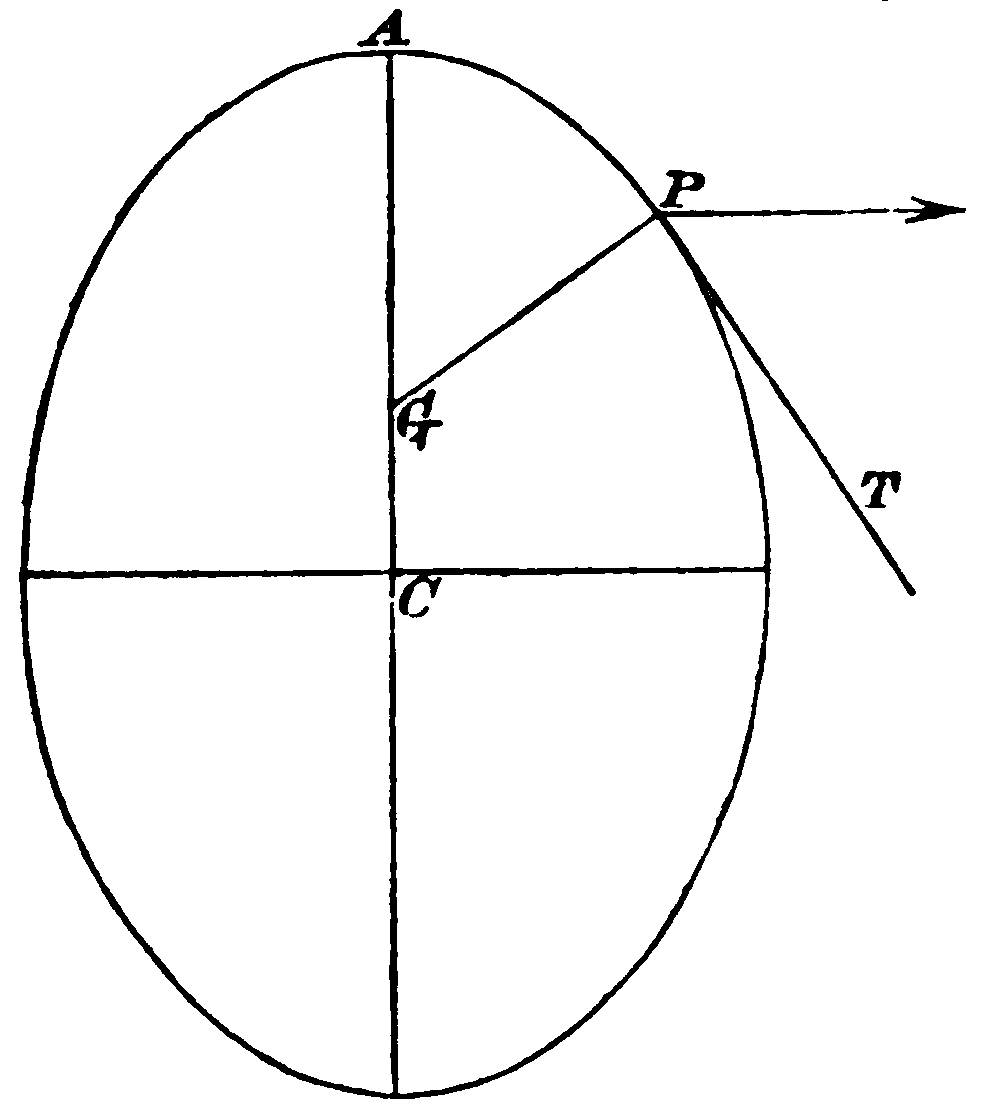
\includegraphics[width=0.49\textwidth]{201.png}
\centering
\end{figure}
oblongum generated by the revolution of this ellipse around
its major-axis.

The attraction of the oblongum at \(P\) will be in a direction
which is \textit{on the same side of \(PG\) as \(PC\) is}; this is obvious, for
the oblongum may be cut up by planes parallel to the tangent-plane
at \(P\) into slices, which all have their centres on the diameter
through \(P\). The so-called centrifugal force at \(P\) will be in a
direction at right angles to \(AC\) outwards. Hence the attraction,
and the so-called centrifugal force, will give rise to a component
along \(PT\); and so the fluid cannot be in relative equilibrium.

\Section
1083. We may observe that on Laplace's page 58 we have
the fraction \(\xp\dfrac{27\lambda + 30\lambda^3 + 7\lambda^5}{(1 + \lambda^2)(3 + \lambda^2)(9 + \lambda^2)}\), which might be reduced to
the simpler form \(\xp\dfrac{\lambda(9 + 7\lambda^2)}{(1 + \lambda^2)(9 + \lambda^2)}\). Poisson also uses the unreduced
form: see his \textit{Traité de Mécanique}, Vol.\ \textsc{ii}.\ page 542.

\Section
1084. If the angular velocity exceeds a certain limit the
oblatum is not a possible figure of relative equilibrium. Laplace
makes an important remark with respect to this on his page 59:
he says that it might have been supposed that this limiting case
%%-----File: 202.png-----%%
is that in which the fluid would begin to fly off by reason of the
too rapid rotatory motion, but it is easily found that this is not
the fact.

Poisson alludes to the matter in the \textit{Connaissance des Tems}
for 1829; he says on page 375, after remarking that within a
certain limit the ellipsoid of revolution is a solution:
\begin{squote}
Si l'ellipsoïde était la seule figure qui eût cette propriété, il en résulterait
cette conséquence singulière que l'équilibre serait impossible pour
une rapidité de la rotation qui n'est pas cependant celle ou le fluide
commencerait à se dissiper.
\end{squote}

\Section
1085. Laplace's theorem that there is only one oblatum corresponding
to a given moment of rotation will be found with a
different demonstration in Resal's work: see his page 198. An
interesting point of analysis is involved.

The problem is reduced to this equation
\[q = (1 + \lambda^2)^{\frac{2}{3}}\frac{(3 + \lambda^2)\tan^{-1}\lambda - 3\lambda}{\lambda^3},\]
where \(q\) is a given positive quantity, and \(\lambda\) has to be found. Then
it is demonstrated that there is one, and only one, value of \(\lambda\)
between \(0\) and infinity which satisfies this equation.

It is easily shewn that there is one value of \(\lambda\) which satisfies
the equation; for the right-hand member vanishes when \(\lambda\)
vanishes, and is infinite when \(\lambda\) is infinite.

Put \(\tan\theta\) for \(\lambda\); then the right-hand member becomes
\[\frac{\theta(1 + 2\cos^2\theta) - 3\sin\theta\cos\theta}{(\cos\theta)^{\frac{1}{3}}\sin^3\theta};\]
we will denote this by \(u\). It will be found that
\[\frac{du}{d\theta} = \frac{9\sin\theta\cos\theta(1 + 2\cos^2\theta) + \theta(1 - 20\cos^2\theta - 8\cos^4\theta)}{3(\cos\theta)^{\frac{4}{3}}\sin^4\theta}.\]

Now Resal in effect puts this expression in the following form:
\[\frac{du}{d\theta} = \frac{1}{3(\cos\theta)^{\frac{4}{3}}}\left\{\theta + \frac{9(2 + \cos^2\theta)}{\sin^4\theta}\cos^2\theta\left[\frac{1 + 2\cos^2\theta}{2 + \cos^2\theta}\tan\theta - \theta\right]\right\}.\]
%%-----File: 203.png-----%%

This is certainly positive provided \(\xp\dfrac{1 + 2 \cos^2 \theta}{2 + \cos^2 \theta} \tan \theta - \theta\) is
positive; and the differential coefficient of the last expression is
found to be positive, so that as the expression vanishes with \(\theta\) it
must always be positive as \(\theta\) changes from \(0\) to \(\xp\dfrac{\pi}{2}\).

Thus \(u\) increases with \(\theta\), and so can only once have an assigned
value as \(\theta\) changes from \(0\) to \(\xp\dfrac{\pi}{2}\).

The point of interest which is involved is the following: if \(a\)
and \(b\) are positive quantities, determine under what conditions
\(\tan \theta\xp\dfrac{ 1 + a \tan^2 \theta}{1 + b \tan^2 \theta} - \theta\) is always positive while \(\theta\) changes from \(0\)
to \(\xp\dfrac{\pi}{2}\).

It will be found that the differential coefficient of the last
expression is
\[\frac{(3a - 3b + 1)\tan^2 \theta + (ab + 3a - b - b^2)\tan^4 \theta + ab \tan^6 \theta}{(1 + b \tan^2 \theta)^2}.\]

Thus the required result is secured if \(3a-3b+1\) and
\(ab+3a-b-b^2\) are both zero or positive. Thus \(a\) must not
be less than \(b - \xp\dfrac{1}{3}\), and \(b\) for perfect security not less than \(\xp\dfrac{3}{5}\).
Therefore if \(a\) is not less than \(\xp\dfrac{4}{15}\) then \(\tan \theta\xp\dfrac{ 1+ a \tan^2 \theta}{1+ \left(a+\dfrac{1}{3}\right)\tan^2 \theta}\)
is greater than \(\theta\), or \(\tan \theta\) is greater than \(\theta + \xp\dfrac{1}{3}\xp\dfrac{ \theta \tan^2 \theta}{1 + a \tan^2 \theta}\).

\Section
1086. I may remark that Bowditch's notes on this Chapter
bring before the reader the peculiar notions which Ivory held
as to fluid equilibrium. Like every other person Bowditch
objects to these notions; but some of his language in his account
of the matter seems to want precision, estimated from our modern
notions. Thus on his page 206 he speaks of the ``forces which
act upon the point \(I\)\,'': if by a point he means a small element of
the fluid we should require to know the form of that element.
Again on page 208 he speaks of ``the effort of the fluid \dots\ to
%%-----File: 204.png-----%%
rise in the branch\dots.'' Perhaps he had fallen a little under the
influence of Ivory.

A note by Bowditch on his page 222 should be observed. A
reader of Laplace might fail to recollect that he uses the revolutionary
mode of reckoning hours, minutes, and seconds.

\Section
1087. Laplace seems to have attached considerable importance
to the proposition that there is only one oblatum corresponding
to a given moment of rotation. See the \textit{Mécanique Céleste},
Vol.\ \textsc{v}.\ page 10, ``mais le véritable problème à résoudre,\dots'' Laplace
had been to some extent anticipated by Thomas Simpson: see
Art.\ 286.

\Section
1088. The fourth Chapter of the Third Book is entitled \textit{De la
figure d'un sphéroïde très-peu différent d'une sphère et recouvert
d'une couche de fluide en équilibre.}

The title of the Chapter seems inadequate; for Laplace discusses
not only the case in which a solid is covered by a film
of fluid, but also the case in which the body is supposed entirely
fluid.

The Chapter is mainly composed of matter which Laplace had
previously published in memoirs. The §§ 22\dots 28 are from the
fourth memoir; the §§ 29 and 30 are from the seventh memoir;
the §§ 31 and 32 are from the fifth memoir; § 33 is from the
fourth memoir, with the exception of the examination of Bouguer's
hypothesis on pages 97\dots 99 which is new; §§ 34 and 35 are new;
§ 36 is substantially in the \textit{Figure des Planetes}; § 37 is new.

\Section
1089. Laplace in his §§ 22\dots 25 treats the case of a homogeneous
body which is nearly spherical and fluid, or covered with a
film of fluid; when this body rotates with uniform angular velocity,
Laplace shews that for relative equilibrium the external surface
of the fluid must be that of an oblatum. He does not \textit{assume}
that the body is a figure of revolution. The demonstration depends
on the use of Laplace's functions. The demonstration is
substantially reproduced by Resal: see his pages 209\dots 211.

Laplace gives in his § 26 another demonstration, very curious,
and not employing Laplace's functions; it does not seem to have
%%-----File: 205.png-----%%
been reproduced in an elementary book. Some remarks on it
will be found in Liouville's \textit{Journal de Mathématiques} for June
and August 1837, and April 1839. Laplace's method in fact
has been shewn to be unsatisfactory; and we shall consider the
matter in a later Chapter.

It will be remembered that Legendre first discussed a case of
this problem in his second memoir: see Chapter \textsc{xxii}.

\Section
1090. Laplace in his §§ 27 and 28 considers the case of a
homogeneous fluid which surrounds a spherical nucleus of a
density different from that of the fluid. A small part of the investigation
is reproduced in Resal's pages 212 and 213.

\Section
1091. Laplace in his §§ 29\dots 31 discusses the figure of the
Earth considered as a heterogeneous fluid. We have already
stated in Art.\ 968 that Laplace made no substantial addition
to the results obtained in Legendre's fourth memoir.

\Section
1092. The most important point in these §§ 29\dots 31 is the
demonstration that in the expression of the radius vector of any
stratum of the body in terms of Laplace's functions, the functions
of a higher order than the second must vanish.

I have discussed the various investigations on this important
point which have been given by Legendre, Laplace, O'Brien, and
Pratt, in a memoir to which I have referred in Art.\ 933.

\Section
1093. Laplace in his § 32 examines the conditions which
follow from supposing that the axis of rotation is a principal
axis. See Art.\ 953.

\Section
1094. Laplace's § 33 is important. He obtains expressions for
the force of gravity, the length of the seconds pendulum, and
the length of a degree of the meridian at an assigned latitude.
He says on his page 97: ``Ces trois expressions ont l'avantage
d'être indépendantes de la constitution intérieure de la terre,
c'est-à-dire, de la figure et de la densité de ses couches;\dots'' He
means that he has only assumed the strata of equal density to
be very nearly spherical.
%%-----File: 206.png-----%%

In this section he shews it is impossible to admit Bouguer's
hypothesis that the variation in the length of a degree of the
meridian is proportional to the fourth power of the sine of the
latitude. For this hypothesis see page 298 of Bouguer's \textit{Figure
de la Terre}. See also Art.\ 924.

\Section
1095. In his § 34 Laplace considers the particular case in
which the body is formed of elliptical strata. This case is that
which holds if the body is assumed to be entirely fluid, as appears
from the §§ 29\dots 31. Laplace moreover shews that this must be
the case if we assume all the strata to be similar and covered
with a film of fluid: this case was discussed by Legendre; see
Art.\ 902.

This section reproduces important results given by Clairaut.
Thus on Laplace's page 101 we have what we find on Clairaut's
page 227: see Art.\ 329. On Laplace's page 102 we have what
we find on Clairaut's page 217: see Art.\ 323. Also on Laplace's
page 102 we have Clairaut's theorem, as on Clairaut's page 250:
see Art.\ 336.

\Section
1096. Laplace in his § 35 shews how to calculate the attraction
exerted on an external particle by a spheroid, the surface of
which is a film of fluid in relative equilibrium. Laplace assumes
still that the strata of equal density are nearly spherical.

\Section
1097. Laplace in his § 36 finds an expression for the force of
gravity, on the supposition that the law of attraction is that of the
\(n^{\mathrm{th}}\) power of the distance, and that the body is nearly spherical
and homogeneous, and rotates with uniform angular velocity: see
Art.\ 816.

\Section
1098. Laplace in his § 37 shews how to extend the approximation
to the square and higher powers of the small quantity \(\alpha\).
This matter is more fully discussed by Poisson in a memoir in the
\textit{Connaissance des Tems} for 1829.

A misprint at the beginning of this section runs throughout
it. The first equation should be
\[\text{constant} = V - \frac{g}{2}r^2\left(\mu^2 - \frac{1}{3}\right) + \frac{1}{3}gr^2.\]
%%-----File: 207.png-----%%

Laplace omits the term \(\xp\dfrac{1}{3}gr^2\). It should be remarked that on
his suppositions the \textit{variable part} of \(\xp\dfrac{1}{3}gr^2\) may be considered as of
the second order; but then he is here retaining terms of the
second order. The mistake is pointed out by Bowditch.

\Section
1099. The fourth Chapter contains, as we see, much that is
important. The §§ 22\dots 28 are Laplace's own, and very valuable.
With respect to the figure of the Earth, considered as a heterogeneous
fluid, we have seen in Art.\ 891 that Legendre claims the
priority.

\Section
1100. The fifth Chapter of the Third Book is entitled \textit{Comparaison
de la théorie précédente, avec les observations.}

This Chapter is principally from Laplace's seventh memoir;
but the following pages are new: 113\dots 125, 141\dots 146, 151\dots 153.

The Chapter consists of two parts; first we have geometrical
investigations mainly relating to geodesic lines on a spheroid
which differs but little from a sphere; and next we have numerical
calculations to determine the figure of the Earth from the
measured lengths of degrees at various points of the Earth's surface,
and from the observed lengths of the seconds pendulum. Both
these subjects have been much developed since Laplace's time.
The geometrical investigations would now be studied to most
advantage in some work on Geodesy; see for instance the sixth
Book of Puissant's \textit{Traité de Géodésie}, third edition, in two quarto
volumes, 1842. The practical measurement of degrees on the
Earth's surface has been carried on with so much energy in recent
times, that the data for numerical computation are now far more
extensive than those accessible to Laplace. See for instance the
modern works on the English, the Russian, and the Indian
surveys.

I may observe that Resal on his pages 244\dots 262 gives geometrical
investigations of about the same extent as Laplace's,
but by a different method: these would be interesting if they
were not so inaccurately printed as to be scarcely intelligible.
%%-----File: 208.png-----%%

\Section
1101. Laplace's pages 109\dots 111 consist of generalities about
geodesic lines; they might with advantage be put into a more
modern shape.

Pages 112\dots 114 contain formulæ suited to the case of a nearly
spherical body.

Pages 115\dots 117 treat of the special case in which the geodesic
line starts by being parallel to the corresponding plane of the
celestial meridian.

Pages 118\dots 122 treat of the special case in which the geodesic
line starts by being at right angles to the corresponding plane of
the celestial meridian.

Pages 123\dots 126 treat of the radius of curvature of a geodesic
line.

\Section
1102. We may observe that there is a misprint on Laplace's
page 119. He twice puts \(\alpha\) before \(\xp\dfrac{{ddu_{\invprime}}'}{d\phi d\psi}\) when it ought not to be
there. The misprint was pointed out by Bowditch on his page 394.
The misprint is preserved in the national edition of Laplace's
works: see the page 139.

Another misprint occurs on Laplace's page 125, and on the
corresponding page, namely 146, of the national edition.

Laplace takes for the radius vector of a certain ellipsoid
\[1 - \alpha\sin^2 \psi\{1 + h\cos 2(\phi + \beta)\},\]
when it should be
\[1 - \alpha\sin^2 \psi\{1 + h \cos 2(\phi + \beta)\} + \alpha h\cos 2(\phi + \beta);\]
and in consequence he gives erroneous expressions for the lengths
of a degree. For example, he gives for the degree measured perpendicular
to the meridian
\[1° + 1°\ldot\alpha \{1 + h\cos 2(\phi + \beta)\} \sin^2\psi + 4°\alpha h \tan^2 \psi \cos 2(\phi + \beta),\]
when it should be
\[1° + 1°\ldot\alpha \{1 + h\cos 2(\phi + \beta)\} \sin^2\psi - 3°\alpha h\cos 2(\phi + \beta).\]

The corrections were pointed out by Bowditch on his pages
412\dots 416.
%%-----File: 209.png-----%%

The corrections are adopted by Puissant: see Vol.\ \textsc{ii}.\ pages
393\dots 395 of the work cited in Art.\ 1100.

\Section
1103. We now proceed to the second of the two parts which
compose Laplace's fifth Chapter; namely, the numerical calculations
as to the figure of the Earth. The various measured lengths
of degrees do not agree in giving precisely the same value to the
numerical elements of the figure of the Earth; so it is a subject
of enquiry to determine the best method of treating the data
which are furnished by observation.

Laplace proposes two different methods for treating discordant
observations, neither method being that which is known as the
method of least squares. The first method is given in his § 39
and the second in his § 40.

\Section
1104. Let us first consider the method of § 39. Suppose
\(a_1\), \(a_2\), \(a_3\), \dots\ measured lengths of a degree in different latitudes,
and \(p_1\), \(p_2\), \(p_3\), the corresponding squares of the sines of the
latitude. If the Earth were accurately an oblatum, and there
were no errors of observation, we should have a series of equations
of which the type would be, neglecting the square of the
ellipticity,
\[a_r- z - yp_r = 0 \tag{15}.\]

But as there will be errors of observation we shall have instead
of zero on the right-hand side, an unknown error, which we will
denote by \(e_r\). So that the general type of the equations will be
\[a_r - z - yp_r = e_r \tag{16}.\]

Laplace proposes that we should determine \(y\) and \(z\) by the
condition that the numerically greatest of the quantities \(e_1\), \(e_2\), \dots\
should have the least numerical value. See Arts.\ 960 and 961.

Laplace sketches a general process of solution which would
apply if there were more than \textit{two} quantities to be found like
\(y\) and \(z\); and then he discusses with greater detail the solution
for the actual case.

The problem may be stated verbally thus: to determine the
elliptic figure of the Earth so that the greatest deviation from
observation may have the least possible value.
%%-----File: 210.png-----%%

From examining equations (15) and (16) we see that the problem
which Laplace solves may be put in the following geometrical
form: a system of straight lines in a plane is given,
required to find the point which has the least possible value for
the \textit{relative} distance from the straight line which is most remote
from it. By the \textit{relative} distance is here meant the distance
measured in a direction which is fixed for each straight line, though
in general not the same for any two straight lines.

\Section
1105. Laplace's § 40 is devoted to another method of treating
the observations. He now proposes to determine the generating
ellipse of the Earth's figure by the two conditions that the
sum of all the errors is zero, and that the sum of all the errors
taken positively is a minimum. Laplace calls this the most
probable ellipse. The method is due to Boscovich: see Art.\ 962.

\Section
1106. Bowditch thinks that the method of Boscovich ``is
not now so much used as it ought to be'': see page 434 of the
second volume of his translation of the \textit{Mécanique Céleste}.
Bowditch objects to the method of least squares as commonly
applied to the problem, and proposes a modification of it.

I presume that neither of the two methods which Laplace
discusses would now be practically used in such calculations,
but the method of least squares.

\Section
1107. Laplace's § 41 gives numerical application. He takes
seven measures of degrees, and calculates a result by both the
methods he has explained: see Art.\ 961.

Laplace comes to the conclusion that the errors which are
thus found in the observations are too large to allow us to adopt
the supposition that the figure of the Earth is an oblatum.

Laplace corroborates his opinion that the Earth is not an
oblatum, by considering especially the results of operations which
had been recently carried on by Delambre and Méchain, for measuring
an arc of the meridian between Dunkirk and Barcelona.
He applies the method of his § 39; and arrives at an ellipticity
of \(\xp\dfrac{1}{150}\), which cannot be reconciled with the phenomena of gravity
and of precession and nutation.
%%-----File: 211.png-----%%

Laplace finds the length of a quarter of the terrestrial meridian.
He uses the ellipticity \(\xp\dfrac{1}{334}\) which he obtains by combining
the French measure of an arc of the meridian with the
measure of the arc in Peru. He also settles the length of a
metre, defined to be \(\xp\dfrac{1}{10000000}\) of a quarter of the meridian, in
terms of the \textit{toise of Peru}.

\Section
1108. Laplace in his § 42 discusses the observed lengths of
pendulums; he takes fifteen cases: see Art.\ 965.

\Section
1109. Laplace's § 43 is devoted to Jupiter. Assuming that
the planet is a homogeneous fluid he determines the ellipticity;
he finds that the equatorial diameter would then be to the polar
diameter as 1·10967 is to 1.

By a weak analogy from the form of Jupiter Laplace infers
that the Earth's ellipticity is less than \(\xp\dfrac{1}{300}\).

\Section
1110. There are numerical mistakes on Laplace's pages 139,
142, 148, and 150; the corresponding pages of the national
edition are 163, 166, 173, and 175 respectively, where the mistakes
are reproduced: the corrections are given by Bowditch on
his pages 447, 459, 471 and 477 respectively.

\Section
1111. Laplace on his page 140 considers that an error so
great as 48·6 double toises cannot have occurred in the arcs measured
in Pennsylvania, at the Cape of Good Hope, and in Lapland;
and again on his page 141 he considers that an error of
86·26 double toises in the Lapland degree is much too great to
be admitted.

If we accept Svanberg's measurement of the arc in Lapland,
the error in the original determination of the length of a centesimal
degree, which Laplace here uses, is about 200 toises, which
exceeds that which Laplace pronounced too great to be admitted:
see Art.\ 197.

As to the arc in Pennsylvania, Bowditch, himself an American,
proposes to reject it: see his page 444.
%%-----File: 212.png-----%%

\Section
1112. I do not quite follow some remarks made by Laplace
on his page 143. He uses four measured arcs of meridian from
the recent French operations; and from these by the application
of his § 39 he deduces an ellipticity of about \(\xp\dfrac{1}{150}\). Then he
shews that this also agrees well with an arc measured perpendicular
to the meridian in England. So that on the whole the
result may be said to depend on \textit{four} French arcs of meridian,
and \textit{one} English arc perpendicular to the meridian.

Now Laplace says:
\begin{squote}
Mais il est très-remarquable, que les mesures faites nouvellement en
France et en Angleterre, avec une grande précision, dans le sens des
méridiens, et dans le sens perpendiculaire aux meridiens, se réunissent
à indiquer un ellipsoïde osculateur dont l'ellipticité est \(\xp\dfrac{1}{150}\),\dots
\end{squote}

On this I remark that Laplace's words would seem to suggest
that to get this result he had used both French and English arcs
of the meridian, and both French and English arcs perpendicular
to the meridian; instead of what he really did use. And again
he now seems to consider this as the \textit{most probable result} of the
observations, whereas he has himself in his § 40 given that
name to a different result and obtained on different principles.
This may be illustrated by his calculations with respect to the
seven selected degrees of § 41. By the method of § 39 Laplace
obtains an ellipticity \(\xp\dfrac{1}{277}\), which should have been \(\xp\dfrac{1}{250}\) as
Bowditch shews: by the method of § 40 Laplace obtains an ellipticity
\(\xp\dfrac{1}{312}\), which is very different from the former.

\Section
1113. On his page 147 Laplace notices \textit{fifteen} pendulum
observations. Of these he seems to make two divisions, one containing
\textit{nine} and the other \textit{eight}: it seems to me that his second
division contains only \textit{six}.

\Section
1114. On his page 151 Laplace incautiously makes the length
of the seconds pendulum vary as the square of the latitude. It
%%-----File: 213.png-----%%
should be that the \textit{increment} of the length varies as the square of
the sine of the latitude.

\Section
1115. The geometrical investigations which constitute § 38
of this Chapter seem to be Laplace's own; at least I have not
discovered them in any preceding writer. The method of § 39
seems also his own. The method of § 40 is due to Boscovich, as
we have seen in Art.\ 962. The § 38 is the only part which can
be considered now to constitute an essential part of the subject;
it consists of the geometrical investigations which we noticed in
Art.\ 1100. The numerical calculations which form the latter part
of the Chapter by their nature could only have a temporary value;
and they are now superseded by more elaborate work founded
on a more extensive supply of measurements and observations.

\Section
1116. The sixth Chapter of the Third Book is entitled \textit{De la
figure de l'anneau de Saturne.}

The § 44 of this Chapter differs from the corresponding part
of Laplace's sixth memoir; but the §§ 45 and 46, which constitute
the main part of the Chapter, are substantially the same here as
in the memoir.

We may observe that a sketch of the history of the subject, so
far as we have gone up to the end of the fifth Chapter, is given
by Laplace himself in the pages 1\dots 11 of the fifth volume of the
\textit{Mécanique Céleste}: on pages 288\dots 291 he gives a sketch of the
labours of Astronomers and Geometers as to the ring of Saturn;
we may notice especially the top of page 290. It is stated on
page 288 that Herschel saw only \textit{two} rings. This is contrary to
what Laplace had anticipated in his sixth memoir.

\Section
1117. Laplace says towards the beginning of his § 44 that
he will consider a thin stratum of fluid spread over the surface of
the rings to be in equilibrium; and he says at the beginning of
§ 45 that he will consider the ring to be a homogeneous fluid mass.
However the two hypotheses come to the same thing; for if we
regard the ring as fluid, then, the forces being such as occur in
nature, if the condition for the equilibrium of the surface is satisfied,
the mass will be in equilibrium throughout.
%%-----File: 214.png-----%%

\Section
1118. Laplace does not say distinctly what is the order of
approximation which he adopts. The fact is that he replaces
a ring by an infinite right cylinder; and he gives no investigation
by which we can judge of the amount of error which this involves.
The suggestion he makes that we should put
\[
V = V' + \frac{1}{a}V'' + \frac{1}{a^2}V''' + \ldots,
\]
where \(a\) is the distance between the centre of Saturn and the
centre of the generating curve of the ring, and thus get \(V\) in a
series, seems of no practical value.

\Section
1119. Laplace then really determines the attraction of an
infinite cylinder on an external particle. Take the axis of \(z\)
parallel to the generating lines of the cylinder. Then the potential
\(V\) must satisfy the equation
\[
\frac{d^2 V}{dx^2} + \frac{d^2 V}{dy^2} = 0;
\]
therefore
\[
V = f(x + y\xsurdm{-1}) + F(x - y\xsurdm{ -1}),
\]
where \(f\) and \(F\) denote functions at present arbitrary.

Suppose that from symmetry we know that a change in the
sign of \(y\) will not change \(V\); then
\[
V = f(x - y\xsurdm{ -1}) + F(x + y\xsurdm{ -1}).
\]

Therefore by addition
\[\begin{aligned}
V &= \frac{1}{2}\{f(x + y\xsurdm{ -1}) + F(x + y\xsurdm{ -1})\}\\
&+ \frac{1}{2}\{f(x - y\xsurdm{ -1}) + F(x - y\xsurdm{ -1})\}\\
&= \phi(x + y\xsurdm{ -1}) + \phi(x - y\xsurdm{ -1}) \quad \text{say.}
\end{aligned}\]

Hence if we find the value of \(V\) for the case in which \(y = 0\),
we can infer the general value of \(V\). Or if we find the value of
\(\xp\dfrac{dV}{dx}\) when \(y = 0\), we shall in fact determine \(\phi'(t)\) when \(t = x\); then
we can deduce the value of \(\phi'(t)\) when \(t = x \pm y\xsurdm{ -1}\).

See the last paragraph of Art.\ 1048.

\Section
1120. We may thus confine ourselves to estimating the
attraction of an elliptic cylinder on an external particle, which
%%-----File: 215.png-----%%
is in one of the principal planes that contain the axis of the
cylinder. Suppose the cylinder decomposed into rods, parallel
to the generating lines, of infinitesimal section. The attraction of
an infinite straight line we know is represented by \(\xp\dfrac{2}{p}\), where \(p\) is
the perpendicular from the point on the line.

Let the diagram represent a section of the cylinder by a plane
at right angles to the axis, and passing through the attracted
\begin{figure}[ht!]
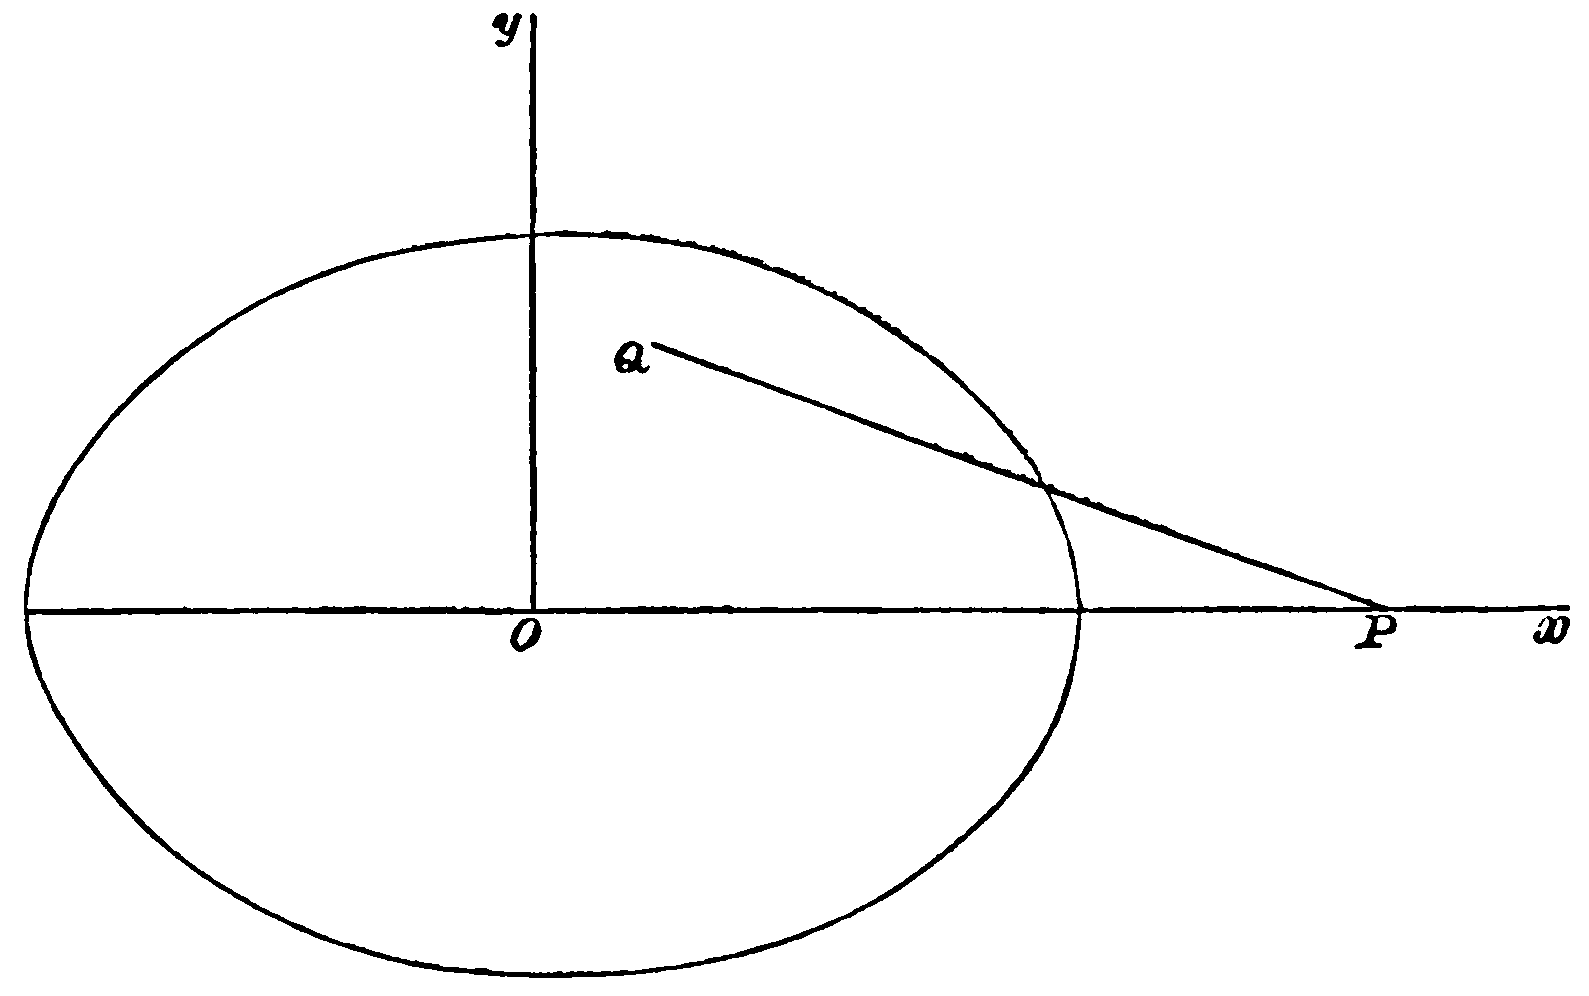
\includegraphics[width=0.78\textwidth]{215.png}
\centering
\end{figure}
particle \(P\), which is on one of the axes of the elliptic section produced.
Let \(O\) be the centre of the ellipse, \(OP = u\). The attraction
of the rod corresponding to \(Q\) may be denoted by \(\xp\dfrac{2dxdy}{PQ}\);
this is along \(PQ\). Resolve this, and we obtain for the attraction
along the axis of \(x\)
\[\frac{2dx\,dy\, (u - x)}{y^2 + (u - x)^2}.\]

Hence the resultant attraction of the cylinder is along the axis
of \(x\), and its value is
\[2\iint \frac{(u - x)\,dx\,dy}{y^2 + (u - x)^2};\]
the integration is to extend over the whole area of the ellipse,
the equation of which may be denoted by \(x^2 + \lambda^2 y^2 = k^2\).

Laplace integrates with respect to \(y\), and then states what the
integration with respect to \(x\) will give.
%%-----File: 216.png-----%%

\Section
1121. We may conveniently use polar coordinates in evaluating
the definite integral of the preceding Article. Let
\[u - x = r \cos\theta,\qquad y = r \sin\theta.\]

Then the definite integral becomes
\[2\iint \frac{r\cos\theta \ldot r\, dr\, d\theta}{r^2}\text{,\quad that is\quad}2\iint \cos\theta \,dr \,d\theta;\]
and the limits are to be found from the equation
\[(u - r\cos\theta)^2 + \lambda^2 r^2 \sin^2\theta = k^2,\]
that is
\[r^2(\cos^2 \theta + \lambda^2 \sin^2 \theta) - 2ur\cos\theta + u^2 - k^2 = 0\tag{17}.\]

Integrate first with respect to \(r\), and use the limits which will
be furnished by the last equation, thus we obtain
\[4\int\frac{\cos\theta \xsurd\{u^2 \cos^2 \theta - (u^2 - k^2)(\lambda^2\sin^2 \theta + \cos^2\theta)\} d\theta}{\lambda^2\sin^2 \theta + \cos^2 \theta}.\]

Denote this by \(4v\). Then
\[\begin{aligned}
\frac{dv}{dk} &= \int\frac{k \cos\theta\, d\theta}{\xsurd\{u^2\cos^2\theta - (u^2 - k^2)(\lambda^2\sin^2 \theta + \cos^2\theta)\}}\\
&= \int\frac{k\cos\theta\, d\theta}{\xsurd(k^2 - c^2\sin^2\theta)},
\end{aligned}\]
where \(c^2 = \lambda^2 u^2 + (1 - \lambda^2)k^2\).

The limits of \(\theta\) are the values of \(\theta\) for which the two values of
\(r\) furnished by (17) become equal; it will be found that these are
such as make \(k^2 - c^2 \sin^2 \theta = 0\).

Therefore
\[\frac{dv}{dk} = \frac{\pi k}{c} = \frac{\pi k}{\xsurd\{\lambda^2 u^2 + (1 - \lambda^2)k^2\}}.\]

Hence we can obtain \(v\); and as \(v\) obviously vanishes with \(k\)
we have
\[v = \frac{\pi}{1 - \lambda^2}\left[\xsurd\left\{\lambda^2 u^2 + (1 - \lambda^2)k^2\right\} - \lambda u\right].\]
And the required attraction is \(4v\).

\Section
1122. We have in fact in Arts.\ 1119\dots 1121 a complete account
of the attraction of an infinite cylinder on an external
%%-----File: 217.png-----%%
particle. As to the action of a cylindrical shell it may be shewn
by the aid of Art.\ 215 of the \textit{Statics} that if the surfaces are
similar and similarly situated elliptical cylinders, with a common
axis, the attraction on an internal particle is zero.

\Section
1123. Laplace however really requires the attraction of an
infinite cylinder only for a point at its surface; and this may be
found more briefly. Resolve the cylinder as before into rods,
parallel to the generating lines, of infinitesimal section. Take the
point on the surface as the origin of polar coordinates. Then for
the resolved attractions in two directions at right angles to each
other in a plane at right angles to the axis of the cylinder we
have the expressions
\[X = 2 \iint dr \,d\theta \cos\theta,\qquad Y = 2 \iint dr\, d\theta \sin\theta.\]

Suppose the cylinder an elliptic cylinder. Let \(h\), \(k\) be the
coordinates, referred to the centre as the origin, of the point on
the surface at which the attraction is required; let \(2a\) and \(2b\) be
the corresponding axes of the ellipse. Then the integration with
respect to \(r\) is to be taken from \(r=0\) to
\[r = - \frac{\dfrac{2h \cos\theta}{a^2} + \dfrac{2k\sin\theta}{b^2}}{\dfrac{\cos^2\theta}{a^2} + \dfrac{\sin^2\theta}{b^2}}.\]

The limits with respect to \(\theta\) are \(\theta_{1}\) and \(\theta_{1} + \pi\), where \(\theta_{1}\) is
such that
\[\frac{h\cos\theta_{1}}{a^2} + \frac{k\sin\theta_{1}}{b^2} = 0.\]

Hence we get
\[\begin{aligned}
X &= - \int \frac{4hb^2\cos^2\theta\, d\theta}{a^2\sin^2\theta + b^2\cos^2\theta},\\
Y &= - \int \frac{4ka^2\sin^2\theta\, d\theta}{a^2\sin^2\theta + b^2\cos^2\theta}.
\end{aligned}\]

Therefore
\[\frac{X}{h} + \frac{Y}{k} = -4 \int_{\theta_{1}}^{\theta_{1} + \pi} d\theta = -4\pi.\]
%%-----File: 218.png-----%%

And
\[\begin{aligned}
\frac{Xa^2}{h} + \frac{Yb^2}{k} &= - 4a^2b^2 \int_{\theta_{1}}^{\theta_{1} + \pi}
\frac{d\theta}{a^2\sin^2\theta + b^2\cos^2\theta}\\
&= - 4ab\pi.
\end{aligned}\]

Hence, finally,
\[
X = - \frac{4\pi bh}{a+b}, \qquad Y = - \frac{4\pi ak}{a+b}.
\]

Therefore
\[
X^2 + Y^2 = \left(\frac{4\pi}{a+b}\right)^2 (b^2h^2 + a^2k^2)
= \left(\frac{4\pi ab}{a + b}\right)^2;
\]
thus the resultant is constant for all points of the surface of the
cylinder.

I cannot find that this simple remark has been made before,
though many persons give the formulae for \(X\) and \(Y\); as for
instance Laplace in 1787, and Plana in 1819: see also Resal,
page 155, and Price's \textit{Infinitesimal Calculus}, Vol.\ \textsc{iii}.\ page 289.

The \textit{direction} of the resultant attraction at any point of the surface
can be readily assigned; the tangent of the angle which this
direction makes with the axis of \(x\) is equal to \(\xp\dfrac{Y}{X}\), that is to \(\xp\dfrac{ak}{bh}\).
Hence the direction is parallel to the corresponding radius of the
auxiliary circle.

\Section
1124. The substance of Laplace's Chapter on Saturn's ring is
reproduced by Resal in his pages 239\dots 243.

\Section
1125. The Chapter devoted by Laplace to Saturn's ring is
original and interesting; but it does not discuss the subject
very fully. The reader who desires to obtain information on this
matter will consult the essay by Professor Maxwell, entitled
\textit{On the Stability of the Motion of Saturn's Rings}, Cambridge,
1859: for an account of this essay see the \textit{Monthly Notices
of the Royal Astronomical Society}, Vol.\ \textsc{xix}.\ page 297.

\Section
1126. The seventh Chapter of the Third Book is entitled \textit{De
la figure des atmosphères des corps célestes}.

This occupies little more than three pages of the \textit{Mécanique
Céleste}. Laplace really adds nothing to what was previously known,
%%-----File: 219.png-----%%
and which may be found in the sixth volume of D'Alembert's
\textit{Opuscules Mathématiques}: see Art.\ 639.

It does not seem to me that the Chapter is very clearly
written. Laplace for instance says that at the exterior surface
\(\Pi = 0\); this would be true if the atmosphere were an incompressible
fluid, but for an \textit{atmosphere} we cannot have \(\Pi = 0\), for
as long as there is density there will be pressure. In what
follows Laplace gives the equation
\[
c = \frac{2}{r} + \alpha r^2 \sin^2\theta
\]
as the equation to the \textit{surface} of the atmosphere; but this is
really the equation to any surface of equal pressure.

Laplace afterwards says that the greatest value which the
radius vector can have is that where the centrifugal force is
equal to the attraction; and this is true, and gives a limit to
the extent of the surface.

The subject is treated by Resal in his pages 263\dots 289; he
follows the method and principles of E. Roche to whom he refers.
The substance of Laplace's Chapter is reproduced in Pratt's \textit{Mechanical
Philosophy}, second edition, pages 552\dots 554.

\Section
1127. Here we finish our account of the contributions to our
subject which are contained in the first two volumes of the
\textit{Mécanique Céleste}. They consist of the investigations, collected
and improved, which Laplace made during the last quarter of the
eighteenth century. Their illustrious author combined the highest
mathematical ability with unwearied energy; and he availed
himself of the labours of his predecessors, and of his eminent
contemporary Legendre. He may be said to have received the
theories of Attraction and of the Figure of the Earth immediately
from the hands of D'Alembert; and he transmitted them to his
successors stamped with the permanent impression of his own
genius. Although more than seventy years have elapsed since
the publication of the earlier volumes of the \textit{Mécanique Céleste},
they still embody in their pages the standard treatise on those
parts of Physical Astronomy of which our history treats.
%%-----File: 220.png-----%%

\Chapter{CHAPTER XXIX.}
\Subhead{LAPLACE'S THEOREM.}
\Runhead{\textsc{laplace's theorem.}}

\Section
1128. \textsc{We} shall now proceed to give an account of investigations
which have appeared since the publication of the second
volume of the \textit{Mécanique Céleste}. We shall consider in separate
Chapters the various important points which have been thus discussed.
The present Chapter is devoted to Laplace's theorem
respecting the attractions of confocal ellipsoids.

\Section
1129. We have already noticed Laplace's own demonstration,
which first appeared in his treatise of 1784, was improved
in his fourth memoir, and finally introduced in the \textit{Mécanique
Céleste}: see Arts.\ 804 and 850. Legendre in his third memoir
arrived at the result by a laborious investigation which does not
employ infinite series: see Chapter \textsc{xxiv.}

\Section
1130. We have first to consider a memoir by Biot, entitled
\textit{Recherches sur le calcul aux différences partielles, et sur les attractions
des sphéroïdes}; this is contained in the sixth volume of the
\textit{Mémoires de l'Institut} \dots\ Paris 1806: the memoir occupies pages
201\dots 218 of the volume.

\Section
1131. Biot refers to the researches on the subject of the attraction
of spheroids by Laplace, Lagrange, and Legendre, before
he develops his own method. Let \(V\) be the potential of a given
body on a particle whose coordinates are \(a\), \(b\), \(c\). Biot starts with
the equation
\[
\frac{d^2V}{da^2} + \frac{d^2V}{db^2} + \frac{d^2V}{dc^2} = 0 \tag{1}.
\]

He seems to describe his own method by saying that instead
of trying to integrate this partial differential equation he interprets
%%-----File: 221.png-----%%
the differential form directly. I should describe it by saying
that instead of trying to integrate this differential equation in
finite terms he uses an integral in the form of an infinite series.

\Section
1132. We may transform (1) by substituting three new
variables \(a'\), \(b'\), \(c'\) which are connected with \(a\), \(b\), \(c\) by the arbitrary
equations
\[
a' = F(a, b, c), \quad b' = F_{1}(a, b, c), \quad c' = F_{2}(a, b, c) \tag{2}.
\]

Let \(V'\) denote the form which \(V\) assumes when for \(a\), \(b\), \(c\) we
substitute their values in terms of \(a'\), \(b'\), \(c'\) given by (2). Then
\[
\frac{dV}{da} = \frac{dV'}{da'} \frac{da'}{da} + \frac{dV'}{db'} \frac{db'}{da} + \frac{dV'}{dc'} \frac{dc'}{da} \tag{3},
\]
and similar expressions hold for \(\xp\dfrac{dV}{db}\) and \(\xp\dfrac{dV}{dc}\).

Similarly we can express \(\xp\dfrac{d^2V}{da^2}\), \(\xp\dfrac{d^2V}{db^2}\), and \(\xp\dfrac{d^2V}{dc^2}\).

Then substitute in (1) and we have a partial differential equation
of the second order which we will denote by
\[
L = 0 \tag{4}.
\]

The equation (4) like (1) will be linear.

Suppose the value of \(V'\) which satisfies (4) to be expanded in
powers of \(a'\); say
\[
V' = \phi + a'\phi_{1} + \frac{a'^2}{\oldfactorial{2}} \phi_{2} + \frac{a'^3}{\oldfactorial{3}} \phi_{3} + \frac{a'^4}{\oldfactorial{4}} \phi_{4} + \ldots, \tag{5}
\]
where \(\phi\), \(\phi_{1}\), \(\phi_{2}\), \dots\ denote functions of \(b'\) and \(c'\) which do not contain
\(a'\).

From (5) we must obtain \(\xp\dfrac{dV'}{da'}\), \(\xp\dfrac{dV'}{db'}\), \(\xp\dfrac{dV'}{dc'}\), and the differential
coefficients of \(V'\) of the second order, and substitute these
in (4). Equate to zero the coefficients of the various powers
of \(a'\). Thus we shall have equations which will determine \(\phi_{2}\), \(\phi_{3}\),
\(\phi_{4}\), \dots\ in terms of \(\phi\) and \(\phi_{1}\), but these will remain quite arbitrary.

This is the main part of Biot's investigation. It is obvious
that it is not quite satisfactory. For possibly exceptions might
%%-----File: 222.png-----%%
arise when special forms are assigned to the functions denoted
by the \(F\), \(F_{1}\), \(F_{2}\) of equation (2). Moreover there is nothing to
ensure the convergence of (5).

\Section
1133. From equation (5) we have
\[
\begin{aligned}
\frac{dV'}{da'} &= \phi_{1} + a'\phi_{2} + \frac{a'^2}{\oldfactorial{2}} \phi_{3} + \frac{a'^3}{\oldfactorial{3}} \phi_{4} + \ldots\\
\frac{dV'}{db'} &= \frac{d\phi}{db'} + a'\frac{d\phi_{1}}{db'} + \frac{a'^2}{\oldfactorial{2}}\frac{d\phi_{2}}{db'} + \frac{a'^3}{\oldfactorial{3}}\frac{d\phi_{3}}{db'} + \ldots\\
\frac{dV'}{dc'} &= \frac{d\phi}{dc'} + a'\frac{d\phi_{1}}{dc'} + \frac{a'^2}{\oldfactorial{2}}\frac{d\phi_{2}}{dc'} + \frac{a'^3}{\oldfactorial{3}}\frac{d\phi_{3}}{dc'} + \ldots
\end{aligned}
\]

But in the values of \(\phi_{2}\), \(\phi_{3}\), \(\phi_{4}\), \dots\ we shall find that the function
\(\phi\) itself does not occur but only the differential coefficients of \(\phi\);
this arises from the fact that \(V'\) itself does not occur in (4) but
only the differential coefficients of \(V'\).

Hence the three series just given will be completely determined,
when the first terms are known, that is when the values
of \(\xp\dfrac{dV'}{da'}\), \(\xp\dfrac{dV'}{db'}\), and \(\xp\dfrac{dV'}{dc'}\) are known corresponding to \(a' = 0\).

But these values are connected with the values of \(\xp\dfrac{dV}{da}\), \(\xp\dfrac{dV}{db}\), and
\(\xp\dfrac{dV}{dc}\) by (3) and two similar equations; so we shall have the values
of \(\xp\dfrac{dV'}{da'}\), \(\xp\dfrac{dV'}{db'}\), and \(\xp\dfrac{dV'}{dc'}\) when \(a' = 0\), provided we know the values
of \(\xp\dfrac{dV}{da}\), \(\xp\dfrac{dV}{db}\), and \(\xp\dfrac{dV}{dc}\) when \(a' = 0\).

And as the particular values of \(\xp\dfrac{dV'}{da'}\), \(\xp\dfrac{dV'}{db'}\), and \(\xp\dfrac{dV'}{dc'}\) when
\(a' = 0\), suffice to determine the general values of these differential
coefficients, it follows also that the general values of \(\xp\dfrac{dV}{da}\), \(\xp\dfrac{dV}{db}\), and
\(\xp\dfrac{dV}{dc}\) are determined as soon as we know the particular values which
correspond to \(a' = 0\).
%%-----File: 223.png-----%%

But the equation \(a' = 0\) will represent any surface whatever
by giving the proper form to \(F(a, b, c)\). Hence we obtain the
following very general theorem:

In order to know the attractions of a spheroid at any exterior
points it will be sufficient to know the attractions of this spheroid
at all the points of any exterior surface taken at pleasure.

I have inserted the word \textit{exterior} in Biot's enunciation because
we now know that (1) is not true for internal points.

\Section
1134. As an example we may take for \(a' = 0\) the equation
to the surface of the attracting spheroid itself.

Biot considers that this includes as a particular case Laplace's
theorem respecting ellipsoids. But this becomes more obvious
after some developments to which Biot now proceeds. See
Art.\ 1136.

\Section
1135. If we wish the arbitrary surface to be a plane we may
take \(a = 0\) for its equation. Then it will not be necessary to
transform (1) by the introduction of the new variables \(a'\), \(b'\), \(c'\).
The general value of \(V\) derived from (1) will be
\begin{multline}
V = \phi + a\phi_{1}
- \frac{a^2}{\oldfactorial{2}}\left( \frac{d^2\phi}{db^2} + \frac{d^2\phi}{dc^2}\right)
- \frac{a^3}{\oldfactorial{3}}\left( \frac{d^2\phi_{1}}{db^2} + \frac{d^2\phi_{1}}{dc^2}\right)\\
+ \frac{a^4}{\oldfactorial{4}}\left( \frac{d^4\phi}{db^4}
+ 2\frac{d^4\phi}{db^2dc^2} + \frac{d^4\phi}{dc^4}\right) + \ldots ;\tag{6}
\end{multline}
this may be verified by substituting in (1); or it may be obtained as
in Boole's \textit{Differential Equations}, third edition, pages 401 and 402.

Biot says that this was first given by Lagrange in the \textit{Mécanique
Analytique}, p.\ 474; this means the first edition of Lagrange's
work: see Art.\ 994.

From the above value of \(V\) we can immediately deduce \(\xp\dfrac{dV}{da}\),
\(\xp\dfrac{dV}{db}\), and \(\xp\dfrac{dV}{dc}\).

Biot's result includes that of Laplace relative to symmetrical
spheroids: see Art.\ 1076.
%%-----File: 224.png-----%%

\Section
1136. The preceding developments apply to all kinds of
spheroids; for each particular spheroid the values of \(\phi_{1}\) and \(\xp\dfrac{d\phi}{db}\)
and \(\xp\dfrac{d\phi}{dc}\) will in general be different.

Suppose we take an ellipsoid; the attraction for any point
in the plane of the equator can be obtained, as was shewn in
Legendre's third memoir. We have in this case
\[\phi = MU,\qquad \phi_1 = 0,\]
where \(M\) is the mass of the ellipsoid, and \(U\) is a function which
involves the coordinates of the external point and the \textit{excentricities}
of the ellipsoid; see Art.\ 1060. The result \(\phi_{1} = 0\) follows from
the fact that the ellipsoid is symmetrical with respect to its
equator, and so for any point in that plane the attraction parallel
to the axis of \(a\) must vanish.

Thus for an ellipsoid we obtain from (6)
\[V = MU - \frac{Ma^2}{\oldfactorial{2}} \left(\frac{d^2U}{db^2} + \frac{d^2U}{dc^2}\right) + \frac{Ma^4}{\oldfactorial{4}}\left(\frac{d^4U}{db^4} + 2\frac{d^4U}{db^2 dc^2} + \frac{d^4U}{dc^4}\right)
+ \ldots\]

Hence if there be a second ellipsoid with the same \textit{excentricities},
the value of \(U\) will be the same for both; thus if \(M'\) be the
mass and \(V'\) the potential for the second ellipsoid, we have
\[\frac{V'}{M'} =\frac{ V}{M}.\]
This constitutes the proof of Laplace's theorem.

\Section
1137. Results analogous to those which have been given, but
more simple, hold for the case of spheroids of \textit{revolution}.

For a spheroid of revolution we may put
\[b^2 + c^2 = r^2,\]
and \(V\) will be a function of \(r\) and \(a\).

Thus (1) is transformed into
\[\frac{1}{r} \frac{dV}{dr} + \frac{d^2V}{dr^2} + \frac{d^2V}{da^2} = 0.\]
%%-----File: 225.png-----%%

Hence by the same method as before we arrive at this result:
the attraction of a spheroid of revolution will be known for any
external point whatever, if it is known for every point of any
arbitrary external curve whatever, described in the plane of the
meridian. If we suppose this arbitrary curve to be the prolongation
of the axis we have the result first given by Legendre: see
Art.\ 791.

Biot himself says: ``\dots\ et de là résultent, comme cas particulier,
les beaux théorèmes démontrés pour la première fois par
M. Legendre.'' I do not know what other theorem Biot has in
view besides that to which I have referred.

\Section
1138. I must cite another sentence from Biot's memoir; he
says on page 208, after introducing the function \(V\),
\begin{squote}
M. Lagrange a démontré que les coefficiens différentiels
\[\frac{dV}{da},\quad \frac{dV}{db},\quad \frac{dV}{dc},\]
pris négativement, expriment les attractions exercées par le sphéroïde
sur ce même point, parallèlement aux trois axes rectangulaires. M.
Laplace a fait voir ensuite que la fonction \(V\) est assujetie à l'équation
différentielle partielle
\[\frac{d^2V}{da^2} + \frac{d^2V}{db^2} + \frac{d^2V}{dc^2} = 0.\]
\end{squote}

I do not know on what authority the above expressions for
component attractions are assigned to Lagrange; to me they
appear due to Laplace: see Art.\ 789, and also pages 70 and 133
of Laplace's \textit{Figure des Planetes}.

\Section
1139. Biot's memoir may be said to belong more properly to
the subject of partial differential equations than to that of attractions;
and its interest for us is rather of a speculative than of a
practical character, for it does not really determine the attraction
of any spheroid. So far as Laplace's theorem is concerned, we
see that the investigation is not quite independent, for it borrows
one of the main results of Legendre's abstruse third memoir.

\Section
1140. We arrive now at the remarkable simplification effected
by Ivory. A memoir by him entitled \textit{On the Attractions
%%-----File: 226.png-----%%
of homogeneous Ellipsoids}, was read before the Royal Society on
15th June, 1809; and is printed in the \textit{Philosophical Transactions}
for 1809; it occupies pages 345\dots 372.

\Section
1141. This memoir is famous for containing the enunciation
and demonstration of the theorem which is usually called Ivory's
theorem; but which would be more justly called Ivory's demonstration
of Laplace's theorem. The memoir is the first communicated
by Ivory to the Royal Society; and is I think the best of
all his memoirs which relate to our subject. The memoir forms a
good treatise on the attractions of homogeneous ellipsoids, and
may be read at the present day with interest and profit. There
are two improvements which our modern books present to us;
Ivory makes frequent use of the process of transformation of the
variables in a definite double integral, and this process is now
found to be unnecessary; he treats the attraction on an internal
particle by the method of series, not always convergent, and we
now employ the simple method like that given by Lagrange in
1773, and which is adopted in the \textit{Mécanique Céleste}. It is difficult
to see what induced Ivory to use the method of series, when
Laplace had solved this part of the problem so much better.
The essence of the treatment proposed by Ivory for the attraction
of an ellipsoid on an external particle remains in our elementary
books; and thus it is unnecessary to enter into particulars respecting
it.

\Section
1142. Ivory gives a brief sketch of the history of the subject
in his introductory pages. He refers to the particular cases discussed
by Maclaurin and Legendre, and then passes on to the
more general problem which Laplace attacked. He says:
\begin{squote}
The method of investigation, which La Place has employed for surmounting
the difficulties of this last case, although it is entitled to every
praise for its ingenuity, and the mathematical skill which it displays,
is certainly neither so simple nor so direct, as to leave no room for
perfecting the theory of the attractions of ellipsoids in both these
respects. It consists in shewing that the expressions for the attractions
of an ellipsoid, on any external point, may be resolved into two factors;
of which, one is the mass of the ellipsoid, and the other involves only
%%-----File: 227.png-----%%
the excentricities of the solid and the co-ordinates of the attracted
point: whence it follows, that two ellipsoids, which have the same
excentricities, and their principal sections in the same planes, will
attract the same external point with forces proportional to the masses
of the solids. This theorem includes the extreme case, when the surface
of one of the solids passes through the attracted point: and by
this means the attraction of an ellipsoid, upon a point placed without
it, is made to depend upon the attraction which another ellipsoid,
having the same excentricities as the former, exerts upon a point placed
in the surface. Le Gendre has given a direct demonstration of the
theorem of La Place, by integrating the fluxional expressions of the
attractive forces; a work of no small difficulty, and which is not accomplished
without complicated calculations.
\end{squote}

It will be seen that Ivory speaks of ``the theorem of La
Place'' as I do.

\Section
1143. Ivory's own enunciation of his result is contained in
the following words:
\begin{squote}
If two ellipsoids of the same homogeneous matter have the same
excentricities, and their principal sections in the same planes; the
attractions which one of the ellipsoids exerts upon a point in the
surface of the other, perpendicularly to the planes of the principal
sections, will be to the attractions which the second ellipsoid exerts
upon the corresponding point in the surface of the first, perpendicularly
to the same planes, in the direct proportion of the surfaces, or areas,
of the principal sections to which the attractions are perpendicular.
\end{squote}

The theorem is really the combination of two results both due
to Laplace. One result may be thus expressed: the potentials
of confocal ellipsoids at a given point external to both are as
their masses. The other result is the expression for the attraction
of an ellipsoid on a particle at its surface. See Art.\ 1063.

\Section
1144. A peculiarity in Ivory's memoir is his frequent use of
the process of transformation of the variables in a definite double
integral. Although, as we have seen in Arts.\ 710 and 877,
Lagrange and Legendre had treated of this process, yet I do not
think any good account of it had been given at the time of Ivory's
%%-----File: 228.png-----%%
memoir. However the cases in which he uses the method would
not present any great difficulty.

\Section
1145. On the whole we may say that Ivory's memoir goes
over the same extent of ground as the first Chapter in the Third
Book of the \textit{Mécanique Céleste}; obtaining results equivalent to
Laplace's but in a more simple manner.

We may observe that Ivory refers to Laplace's memoir of 1783
by mistake, instead of 1782; see Ivory's page 347: the mistake
is the same as Legendre makes in his memoir of 1788. Perhaps
Ivory copied it from Legendre: see Art.\ 876.

\Section
1146. The merits of Ivory's process were clearly recognised in
France. Thus Legendre says on page 158 of the \textit{Mémoires de
l'Institut} for 1810:
\begin{squote}
Les difficultés d'analyse que présentait ce problême traité par tant
de moyens différens, disparaissent ainsi tout d'un coup, par le procédé
de M. Yvory, et une théorie qui appartenait à l'analyse la plus abstruse,
peut maintenant être exposée dans toute sa généralité, d'une manière
presque entièrement élémentaire.
\end{squote}

This seems the passage which Dr Thomas Young has in view
though I do not understand his reference involved in the words:
``\dots\ say Legendre and Delambre (\textit{M. Inst.}\ 1812).'' See Young's
\textit{Works}, Vol.\ \textsc{ii}.\ page 581.

\Section
1147. A memoir by Plana entitled \textit{Sulla teoria dell' attrazione
degli sferoidi elittici} is contained in the \textit{Memorie di Matematica
\dots\ della Società Italiana}, Vol.\ \textsc{xv}.\ Modena, 1811. The memoir
occupies pages 370\dots 390 of the first part of the volume. It was
communicated on the 24th November, 1810.

I have already stated that Laplace's proof of his theorem was
published by him in the fourth section of his treatise \textit{De la Figure \dots\
des Planetes}; and afterwards given in an improved form in the
first Chapter of the Third Book of the \textit{Mécanique Céleste}; see
Arts.\ 804 and 1060. Plana's memoir is simply a reproduction of
the section from the treatise \textit{De la Figure \dots\ des Planetes}, a little
expanded by giving the steps of the work in some cases where
%%-----File: 229.png-----%%
Laplace only records the result. Plana probably regarded
Laplace's earlier form of the argument as the more natural,
though the later form is briefer.

Plana's memoir adds nothing to the knowledge of the subject;
though it might save some trouble to young mathematicians in
their study of Laplace's method.

I may draw attention to the following words which occur on
Plana's page 376:
\begin{squote}
\dots\ bellissimo teorema del Sig. \textit{Legendre} mediante il quale, l'attrazione
di un elissoide sopra un punto esteriore alla sua superficie dipende
in ogni caso da quella dei punti situati sulla superficie.
\end{squote}

I cannot admit the propriety of calling this theorem by
Legendre's name; Legendre really established only a part of
this: see Art.\ 782. The extension of the theorem to the generality
thus ascribed to it by Plana is really due to Laplace, being
in fact involved in the theorem which I call by his name.

\Section
1148. A note by Biot entitled \textit{Sur l'attraction des Sphéroïdes}
is given in the \textit{Nouveau Bulletin \dots\ la Société Philomatique} for
March 1812, pages 44\dots 48. This note may be considered as an
appendix to the memoir of 1806.

In the memoir Biot had shewn that the attraction of an ellipsoid
at any external point might be deduced by simple differentiations
from a particular expression, which is theoretically known
when the attraction is known for all points situated in the plane
of one of the principal sections.

Now he says that the demonstration would cease to be applicable
in the case in which the projection of the external point on
the assigned plane falls within the principal section of the ellipsoid.
For the expressions which give the values of the attractions
are different according as the point is within or without the ellipsoid,
and so the results cannot be comprehended in the same
formulæ.

Biot proposes to surmount the difficulty by a transformation
of the coordinates.

Let \(x\), \(y\), \(z\) be the old coordinates of the external point, where
\(x\) and \(y\) refer to the assigned principal plane. Let \(x'\), \(y'\), \(z'\) be the
%%-----File: 230.png-----%%
new coordinates of the point, connected with the old coordinates
by the equations
\[
x' = x + z\tan\alpha \cos\beta,\quad y' = y + z\tan\alpha \sin\beta,\quad z' = z \sec\alpha.
\]

Then the equation (1) of Art.\ 1131 transforms into
\begin{align*}
&(1 + \tan^2 \alpha \cos^2\beta)\frac{d^2 V}{dx'^2} + (1 + \tan^2 \alpha \sin^2 \beta)\frac{d^2 V}{dy'^2}\\
&\quad + \sec^2 \alpha \frac{d^2 V}{dz'^2} + 2\tan^2 \alpha \sin\beta \cos\beta \frac{d^2 V}{dx' dy'}\\
&\quad + 2\tan\alpha \sec\alpha\left(\cos\beta \frac{d^2 V}{dx' dz'} + \sin\beta \frac{d^2 V}{dy' dz'}\right) = 0.
\end{align*}

This is still a linear equation. Hence as in Art.\ 1132 we
find that
\[
V = A_{0} + A_{1} z' + A_{2}\frac{z'^2}{\oldfactorial{2}} + A_{3}\frac{z'^2}{\oldfactorial{3}} + \ldots,
\]
where \(A_{0}\), \(A_{1}\), \(A_{2}\), \dots\ are functions of \(x'\) and \(y'\) Then the inference
is of the same kind as in Art.\ 1133.

We may take \(\alpha\) and \(\beta\) so that \((x', y')\) falls without the ellipsoid,
for the case of any assigned external point. Thus the
difficulty is surmounted.

Although Biot's method in his memoir and in this note is
interesting, yet the use of infinite series of which the convergence
is not secured, cannot be accepted as rigorous.

\Section
1149. We have next to consider a memoir by Legendre
entitled \textit{Mémoire sur l'attraction des ellipsoïdes homogènes}. This is
published in the \textit{Mémoires de l'Institut} for 1810, second part: the
date of publication is 1811. The memoir occupies pages 155\dots 183
of the volume. The memoir was read on the 5th October, 1812.

\Section
1150. Legendre begins by an historical sketch of the subject.
He says that the problem of the attraction of an ellipsoid on an
internal particle had been completely solved with much elegance
by Maclaurin in his prize essay on the Tides. Maclaurin however,
as we have seen, explicitly considered only the case of an
%%-----File: 231.png-----%%
ellipsoid of revolution, though his methods admitted of obvious
extension to the case of the general ellipsoid.

With regard to the attraction of an ellipsoid on an external
particle Legendre adverts to the theorem of Maclaurin: to the
extension which he himself gave of it in the memoir which I
have called his first; to the further extension given by Laplace;
and to his own investigations in the memoir which I have called
his third. He says of the second part of this memoir:
\begin{squote}
J'avoue néanmoins que cette partie de mon Mémoire n'a que le
mérite d'être directe, et de montrer, dès l'abord, la possibilité de la
solution, mais que d'ailleurs l'analyse en est d'une extrême complication.
Il était donc à desirer qu'on découvrît une route plus facile pour parvenir
au même résultat.
\end{squote}

Legendre then refers to Biot for his happy idea of applying to
the equation of the attraction the integral which Lagrange had
given for another object. Legendre says that Biot's result joined
to the first part of his own memoir, the third, completed in a
satisfactory manner the theory of the attraction of homogeneous
ellipsoids; and so there was little hope of acquiring any new degree
of perfection.

But Ivory, whom Legendre calls Yvory, had thrown a fresh
light on the subject by an ingenious transformation. Accordingly
Legendre proposes to avail himself of Ivory's discovery in order to
present the whole theory of the attraction of ellipsoids in its
simplest form. This he effects by combining Ivory's demonstration
with the mode of solution for an internal particle given by
Lagrange, this mode being simpler than that adopted by Ivory,
which depends on development in a series.

\Section
1151. Legendre's memoir forms a very good account of the
attraction of homogeneous ellipsoids; it is clear, simple, and
comprehensive, and might be reprinted at the present time as an
elementary treatise on the subject.

Although there is nothing really new in the methods employed,
yet there are some subordinate results of interest which
appear for the first time, and these we will indicate.
%%-----File: 232.png-----%%

\Section
1152. What we call Ivory's theorem is given by Legendre
substantially in Ivory's manner, though slightly improved. We
need not delay on this, but pass to the case in which the attracted
particle is within the ellipsoid or on its surface.

Let \(a\), \(b\), \(c\) be the semiaxes of the ellipsoid; let \(f\), \(g\), \(h\) be the
corresponding coordinates of an attracted particle; let \(A\), \(B\), \(C\) be
the corresponding resolved parts of the attraction. Then Legendre
shews that
\[\begin{aligned}
A &= 2f \iint \frac{\sin\theta\cos^2\theta \,d\theta \,d\phi}{\cos^2\theta + \dfrac{a^2}{b^2}\sin^2\theta\cos^2\phi + \dfrac{a^2}{c^2}\sin^2\theta\sin^2\phi},\\
B &= \frac{2a^2g}{b^2} \iint \frac{\sin^3\theta\cos^2\phi \,d\theta \,d\phi}{\cos^2\theta + \dfrac{a^2}{b^2}\sin^2\theta\cos^2\phi + \dfrac{a^2}{c^2}\sin^2\theta\sin^2\phi},\\
C &= \frac{2a^2h}{c^2} \iint \frac{\sin^3\theta\sin^2\phi \,d\theta \,d\phi}{\cos^2\theta + \dfrac{a^2}{b^2}\sin^2\theta\cos^2\phi + \dfrac{a^2}{c^2}\sin^2\theta\sin^2\phi}.
\end{aligned}\]
The limits for both \(\theta\) and \(\phi\) are \(0\) and \(\pi\).

Consider the expression for \(A\); the integration with respect
to \(\phi\) can be effected: thus
\[
A = 2f\pi \int\frac{\sin\theta\cos^2\theta \,d\theta}{\bigsurd (\cos^2\theta + \dfrac{a^2}{b^2}\sin^2\theta)
 \bigsurd (\cos^2\theta + \dfrac{a^2}{c^2}\sin^2\theta)}.
\]

Put \(M\) for the volume of the ellipsoid, that is for \(\dfrac{4\pi abc}{3}\).
Also put \(x\) for \(\cos\theta\). Thus we get
\[
A = \frac{3Mf}{a} \int_0^1 \frac{x^2 dx}{\xsurd \{a^2 + (b^2 - a^2)x^2\}
\xsurd \{a^2 + (c^2 - a^2)x^2\} }.
\]

\Section
1153. Now instead of making use of the formulæ given above
for \(B\) and \(C\), we may if we please deduce values of \(B\) and \(C\) from
the value of \(A\), by appropriate changes of the letters. Thus we have
\[
B = \frac{3Mg}{b} \int_{0}^{1} \frac{x^2 dx}{\xsurd \{b^2 + (c^2 - b^2)x^2\}
\xsurd \{b^2 + (a^2 - b^2)x^2\} },
\]
%%-----File: 233.png-----%%
\[
C = \frac{3Mh}{c} \int_{0}^{1} \frac{x^2dx}
{\xsurd \{c^2+(a^2-c^2)x^2\} \xsurd \{c^2+(b^2-c^2)x^2\} }.
\]
All this of course was well known.

Legendre however observes that if we do make use of the
formulæ given in Art.\ 1152 we shall obtain
\[\begin{aligned}
B &= \frac{3Mg}{a(c^2-b^2)}\left[ \frac{c}{b} - \int_{0}^{1} \frac{\xsurd \{a^2+(c^2-a^2)x^2\}\,dx}{\xsurd \{a^2+(b^2-a^2)x^2\} }\right],\\
C &= \frac{3Mh}{a(c^2-b^2)}\left[ - \frac{b}{c} + \int_{0}^{1} \frac{\xsurd \{a^2+(b^2-a^2)x^2\}\,dx}{\xsurd \{a^2+(c^2-a^2)x^2\} }\right].
\end{aligned}\]

Legendre adds that it is easy to convince ourselves that the
different formulæ agree in value. I will supply the process.

\Section
1154. We have in fact by integration by parts
\begin{gather*}
\int \frac{\xsurd \{a^2+(c^2-a^2)x^2\} }{\xsurd \{a^2+(b^2-a^2)x^2\} }\,dx
= \frac{x\xsurd \{a^2+(c^2-a^2)x^2\} }{\xsurd \{a^2+(b^2-a^2)x^2\} }\\
- \int \frac{x^2(c^2-a^2)\,dx}{\xsurd \{a^2+(c^2-a^2)x^2\} \xsurd \{a^2+(b^2-a^2)x^2\} }\\
+ \int \frac{x^2(b^2-a^2) \xsurd \{a^2+(c^2-a^2)x^2\} }{\{a^2+(b^2-a^2)x^2\}^{\frac{3}{2}}} \,dx\\
= \frac{x \xsurd \{a^2+(c^2-a^2)x^2\} }{\xsurd \{a^2+(b^2-a^2)x^2\} }
+ \int \frac{a^2(b^2-c^2)x^2\,dx}{\{a^2+(c^2-a^2)x^2\}^{\frac{1}{2}} \{a^2+(b^2-a^2)x^2\}^{\frac{3}{2}}}.
\end{gather*}

Take the integrals between the limits \(0\) and \(1\); thus we get
from Art.\ 1153
\[
B = 3Mga \int_{0}^{1}
\frac{x^2\,dx}{\{a^2+(c^2-a^2)x^2\}^{\frac{1}{2}} \{a^2+(b^2-a^2)x^2\}^{\frac{3}{2}}},
\]
this is another form for \(B\).

Now put \(\xp\dfrac{x}{\xsurd \{a^2+(b^2-a^2)x^2\} } = \xp\dfrac{y}{b}\); thus
\[
B = \frac{3Mga}{b} \int_{0}^{1} \frac{x^2}{\{a^2+(c^2-a^2)x^2\}^{\frac{1}{2}}}\frac{dy}{a^2};
\]
%%-----File: 234.png-----%%
also \(x^2 = \xp\dfrac{a^2 y^2}{b^2 - (b^2 - a^2) y^2}\), and \(a^2 + (c^2 - a^2) x^2 = \xp\dfrac{a^2 b^2 + a^2 ( c^2 - b^2 ) y^2}{b^2 - (b^2 - a^2) y^2}\);
so that
\[B = \frac{3Mg}{b}\int_0^1 \frac{y^2\, dy}{\xsurd\{b^2 + (c^2 - b^2)y^2\} \xsurd\{b^2 + (a^2 - b^2) y^2\}},\]
which was to be shewn.

\Section
1155. If the ellipsoid differs but little from a sphere we may
obtain an approximation by a series. Take the expression for
\(A\) in Art.\ 1152 as an example.

Let \(\mu = \xp\dfrac{a^2 - b^2}{a^2}\), and \(\nu = \xp\dfrac{a^2 - c^2}{a^2}\). Then
\[A =\frac{3Mf}{a^3} \int_0^1 \frac{x^2\, dx}{\xsurd(1 - \mu x^2)\xsurd(1 - \nu x^2)}.\]

We should expand \textit{before integration}. Let
\[(1 - \mu x^2)^{-\frac{1}{2}} (1 - \nu x^2)^{-\frac{1}{2}} = 1 + P_1 x^2 + P_2 x^4 + P_3 x^6 + \ldots\]

Then it is easy to shew that
\[\begin{aligned}
P_1 &= \frac{1}{2} (\mu + \nu),\\
P_2 &= \frac{1\ldot3}{2\ldot4} (\mu^2 + \nu^2) + \frac{1}{2}\ldot\frac{1}{2}\mu \nu,\\
P_3 &= \frac{1\ldot3\ldot5}{2\ldot4\ldot6} (\mu^3 + \nu^3) + \frac{1\ldot3}{2\ldot4}\ldot\frac{1}{2} \mu \nu (\mu + \nu),\\
P_4 &= \frac{1\ldot3\ldot5\ldot7}{2\ldot4\ldot6\ldot8}(\mu^4 + \nu^4) + \frac{1\ldot3\ldot5}{2\ldot4\ldot6}\ldot\frac{1}{2} \mu \nu (\mu^2 + \nu^2) + \frac{1\ldot3}{2\ldot4}\ldot\frac{1\ldot3}{2\ldot4} \mu^2 \nu^2.\\
\ldots&\ldots\ldots
\end{aligned}\]

The law is obvious.

Thus
\[A = \frac{3Mf}{a^3}\left\{\frac{1}{3} + \frac{1}{5} P_1 + \frac{1}{7} P_2 + \frac{1}{9} P_3 + \ldots\right\}.\]

\Section
1156. If however we wish to avoid series, or if the series are not
convergent, it is convenient to have recourse to elliptic functions.

Let
\[m^2 = b^2 - a^2,\qquad n^2 = c^2 - a^2,\qquad k^2 = 1 - \frac{m^2}{n^2}.\]
%%-----File: 235.png-----%%

In the expression for \(A\) given at the end of Art.\ 1152, put
\(x = \xp\dfrac{a}{n}\tan\phi\); then we get
\[
A = \frac{3Mf}{n^3}\int_0^{\phi_1}
\frac{\tan^2 \phi \,d\phi}{\xsurd(1 - k^2\sin^2 \phi)},
\]
where \(\phi_1\) is such that \(\sin\phi_1=\xp\dfrac{n}{c}\), \(\cos\phi_1=\xp\dfrac{a}{c}\), \(\tan\phi_1 = \xp\dfrac{n}{a}\).

Again, in the expression for \(B\) given at the beginning of
Art.\ 1153 put \(x = \xp\dfrac{b\sin\phi}{n\xsurd(1 - k^2\sin^2 \phi)}\); then we get
\[
B = \frac{3Mg}{n^3}\int_0^{\phi_1} \frac{\sin^2\phi \,d\phi}{(1 - k^2\sin^2\phi)^{\frac{3}{2}}}.
\]

Lastly, in the expression for \(C\) given at the beginning of
Art.\ 1153 put \(x = \xp\dfrac{c\sin\phi}{n}\); then we get
\[
C = \frac{3Mh}{n^3}\int_0^{\phi_1}
\frac{\sin^2 \phi \,d\phi}{\xsurd(1 - k^2\sin^2 \phi)}.
\]

Legendre states the results which are obtained by expressing
the integrals now left in \(A\), \(B\), \(C\) by elliptic integrals: he refers
for the formulæ required to his \textit{Exercices de Calcul Intégral}, 1\textsuperscript{re}
partie, No.\ 138.\ Poisson works out the transformations in his
memoir of 1835, to which I have referred in Art.\ 887.

Thus, to take the simplest of the three expressions for example,
we have
\[
C = \frac{3Mh}{k^2 n^3}\left\{\int_0^{\phi_1}
\frac{d\phi}{\xsurd(1 - k^2\sin^2 \phi)}
- \int_0^{\phi_1}\xsurd(1 - k^2\sin^2 \phi) d\phi \right\}.
\]

\Section
1157. Legendre gives an algebraical relation between \(A\), \(B\),
and \(C\), which he deduces in three ways from his formulæ: we will
take the simplest way. From the formulæ of Art.\ 1152 we
see that
\[
\frac{A}{f} + \frac{B}{g} + \frac{C}{h}
= 2\int_0^\pi \int_0^\pi \sin\theta \,d\theta \,d\phi
= 2\pi\int_0^\pi \sin\theta \,d\theta = 4\pi.
\]

Legendre speaks of this result as an ``équation qui ne paraît
pas avoir été remarquée jusqu'à présent, et qui doit être regardée
comme un théorème nouveau.''
%%-----File: 236.png-----%%

\Section
1158. Legendre gives another result somewhat like that of
the preceding Article; namely
\[\frac{Aa^2}{f} + \frac{Bb^2}{g}+ \frac{Cc^2}{h} = \frac{3M}{n}\int_0^{\phi_1} \frac{d\phi}{\xsurd(1 - k^2 \sin^2 \phi)}\text{:}\]
this he obtains from the values which he has found for \(A\), \(B\), and
\(C\) in terms of elliptic integrals.

It is easy to verify this result; for the formulæ of Art.\ 1152 give
\[\begin{aligned}
\frac{Aa^2}{f} + \frac{Bb^2}{g} + \frac{Cc^2}{h} &= 2a^2\int_0^\pi \hspace{-.5em} \int_0^\pi \hspace{-.5em} \frac{\sin \theta\, d\theta\, d\phi}{\cos^2 \theta + \dfrac{a^2}{b^2} \sin^2 \theta \cos^2 \phi + \dfrac{a^2}{c^2} \sin^2 \theta \sin^2\phi}\\
&\hspace{-.5em}= 2\pi a^2 \int_0^\pi \hspace{-.8em}\frac{\sin \theta\, d\theta}{\bigsurd \hspace{-.2em} \left(\cos^2 \theta + \dfrac{a^2}{b^2} \sin^2 \theta\right) \bigsurd \hspace{-.2em} \left(\cos^2 \theta + \dfrac{a^2}{c^2} \sin^2 \theta\right)}\\
&= 3Ma \int_0^1 \frac{dx}{\xsurd\{a^2 + (b^2 - a^2)x^2\}\xsurd\{a^2 + (c^2 - a^2)x^2\}}.
\end{aligned}\]

Then, as in Art.\ 1156, put \(x = \xp\dfrac{a}{n} \tan \phi\), and the integral becomes
\[\frac{3M}{n}\int_0^{\phi_1} \frac{d\phi}{\xsurd(1 - k^2 \sin^2 \phi)}.\]

\Section
1159. Legendre's memoir is reproduced in his \textit{Exercices de
Calcul Intégral}, Vol.\ \textsc{ii}.\ 1817, pages 512\dots 531, and also in his
\textit{Traité des Fonctions Elliptiques}, Vol.\ \textsc{i}.\ 1825, pages 539\dots 556.
The historical sketch is omitted, and some slight changes occur in
the notation, but the memoir remains substantially as it was
originally. All that is added in these later editions of the memoir
consists of two remarks, of which we will give the substance.

(1) The expressions for \(A\), \(B\), and \(C\) in Art.\ 1156 have an inconvenience
when the ellipsoid differs but little from a sphere;
\(n^3\) is then very small, and as this occurs in the denominators, the
numerators must be calculated with great accuracy. This also
holds with respect to the form of these expressions when two of
the axes of the ellipsoid are equal.
%%-----File: 237.png-----%%

(2) The definite integrals in the expressions for \(A\), \(B\), and \(C\)
depend on only \textit{two} quantities, namely \(k\) and \(\phi_{1}\), although in
general there are six elements involved in the problem, namely
the three semiaxes and the three coordinates of the attracted
particle.

\Section
1160. An account of Ivory's memoir by Poisson is given in
the \textit{Nouveau Bulletin \dots\ la Société Philomatique} for November,
1812, pages 176\dots 180, and for January, 1813, page 216.

This is a clear and satisfactory exposition of the essence of the
memoir of Yvory, as Poisson here spells the name. The following
incidental points may be noticed.

Poisson says that Maclaurin demonstrated his proposition for
points situated on the prolongations of the axes in the case of
solids of revolution. Poisson, like other eminent French mathematicians,
here underestimates what Maclaurin really effected.
See Art.\ 260.

Poisson observes that Ivory treated the attraction on an internal
particle by the method of series; but that it would be better
to adopt the method of direct integration after the manner of
Lagrange. A few days previously Legendre's memoir had been
presented to the French \textit{Institut}, in which Poisson's suggestion
was anticipated.

Poisson extends the range of Ivory's theorem, by shewing that
it is true whatever may be the function of the distance which expresses
the law of attraction; this is now familiar to us, for it has
passed into the elementary books.

Poisson observes that Gauss had recently sent to the \textit{Institut}
an extract from a memoir on the subject; and that he had made
use of the same transformation as Ivory for expressing the coordinates
of a point at the surface of an ellipsoid in terms of two
independent coordinates; see Art.\ 1141. Poisson says: ``Cette
transformation est le point principal de l'analyse de M. Yvory, et
c'est aussi celui de l'analyse de M. Gauss, qui ne paraît pas avoir
eu connaissance du Mémoire du géomètre anglais.''
%%-----File: 238.png-----%%

The transformation to which Poisson refers is, that the equation
\({\dfrac{x^2}{a^2} + \dfrac{y^2}{b^2} + \dfrac{z^2}{c^2} = 1}\) is satisfied by putting
\[x = a \cos \theta,\qquad y = b \sin \theta \sin \phi,\qquad z = c \sin \theta \cos \phi.\]

It may be doubted, however, if we can call this transformation
the principal point in the analysis either of Ivory or of Gauss.
The modern exhibitions of Ivory's theorem do not employ this
transformation.

\Section
1161. Poisson, as we have just seen, was the first to point
out that Ivory's theorem holds when the law of attraction is
expressed by any function of the distance, as well as when the
attraction varies inversely as the square of the distance. The
theorem is now demonstrated with Poisson's extension in elementary
works. Moreover, as I have shewn in my \textit{Statics}, in treating
on Ivory's theorem, the demonstration establishes rather more
than the enunciation states.

The extension which Poisson gave to Ivory's theorem does not
apply to what we call Laplace's theorem; that is to say, it is not
true for any law of attraction that the potentials of confocal ellipsoids
at the same external point are as their masses.

Let \(a_{1}\), \(b_{1}\), and \(c_{1}\) be the semiaxes of an ellipsoid; let \(a_{2}\), \(b_{2}\),
and \(c_{2}\) be the semiaxes of a second ellipsoid confocal with the
former. Let \(P\) denote a point external to both. Let a third ellipsoid
confocal to the former two have the point \(P\) on its surface.
Let \(P_{1}\) denote the point on the first ellipsoid which corresponds
to \(P\), and let \(P_{2}\) denote the point on the second ellipsoid which
corresponds to \(P\).

Let \(E_{1}\), \(E_{2}\), and \(E\) denote the ellipsoids.

Then for any law of attraction we have, estimating the attractions
parallel to the third axes,
\[\frac{\text{Attraction of }E_1\text{ at }P}{\text{Attraction of }E\text{ at }P_1}=\frac{a_1 b_1}{ab},\]
\[\frac{\text{Attraction of }E_2\text{ at }P}{\text{Attraction of }E\text{ at }P_2}=\frac{a_2 b_2}{ab}.\]
%%-----File: 239.png-----%%

Therefore
\[\frac{\text{Attraction of }E_1\text{ at }P}{\text{Attraction of }E_2\text{ at }P}\times\lambda = \frac{a_1 b_1}{a_2 b_2},\]
where \(\lambda\) denotes the ratio of the attraction of \(E\) at \(P_{2}\) to its attraction
at \(P_{1}\). According to the ordinary law of attraction we find
that \(\lambda = \xp\dfrac{c_{2}}{c_{1}}\); this depends on the fact that the attraction of an
ellipsoid on a particle at the surface, estimated perpendicular to a
principal plane, varies as the distance from that plane: this fact
however does not hold for all laws of attraction. It does hold as
we know for the law of the inverse square; and it also holds for
the law of the direct distance.

\Section
1162. We now arrive at a memoir by Gauss entitled \textit{Theoria
attractionis corporum sphaeroidicorum ellipticorum homogeneorum
methodo nova tractata.}

This memoir was communicated to the Royal Society of
Göttingen on the 18th of March, 1813, and published in the
\textit{Comm.\ Societat.\ Reg.\ \dots\ Gott.}\ Vol.\ \textsc{ii}.\ 1813. The memoir occupies
pages 1\dots 22 of Vol.\ \textsc{v}.\ of the collected works of Gauss; and
I have studied it in this reprint. A notice of the memoir by
Gauss himself occupies pages 279\dots 286 of the volume, being
reprinted from the \textit{Göttingische gelehrte Anzeigen} of April, 1813.

This notice is also reprinted in De Zach's \textit{Monatliche Correspondenz},
Vol.\ \textsc{xxvii}.; and there is a German translation of
Gauss's memoir in Vol.\ \textsc{xxviii}.\ of the same series.

\Section
1163. An account of Gauss's method for the attraction of
ellipsoids by Professor Cayley will be found in the \textit{Quarterly
Journal of Mathematics}, Vol.\ \textsc{i}.\ pages 162\dots 166.

\Section
1164. Gauss's writings are distinguished for the combination
of mathematical ability with power of expression: in his hands
Latin and German rival French itself for clearness and precision.

\Section
1165. Gauss gives a short sketch of the history of the problem
of the attraction of ellipsoids. He begins with \textit{ipse summus
%%-----File: 240.png-----%%
Newton}, and then passes to \textit{sagax Maclaurin}; he does not make
the mistake of D'Alembert and others: see Art.\ 260. He refers
to Lagrange's memoirs of 1773 and 1703, to the first and the
third of Legendre's memoirs, to the writings of Laplace, and to
the memoirs by Biot and by Plana, which we have already noticed
in this Chapter. He does not here refer to Ivory, nor to the
memoir by Legendre of 1812: but, as we shall see, he became
acquainted with Ivory's memoir after his own was finished.

\Section
1166. Laplace's proof of his theorem was in the opinion of
Gauss an elegant specimen of analytical skill; but left with
geometers a desire for a more simple and direct method. The
efforts made by Biot and Plana to simplify the discussion must
also be considered very intricate applications of analysis.

\Section
1167. Then with respect to his own solution Gauss says:
\begin{squote}
Gratam itaque analystis atque astronomis fore speramus solutionem
novam problematis celebratissimi per viam plane diversam procedentem,
et ni fallimur ea simplicitate gaudentem, ut nihil amplius desiderandum
linquat.
\end{squote}

Certainly he succeeds completely in his design: his solution is
both simple and elegant.

\Section
1168. Gauss, before he proceeds to the actual problem, gives
various theorems which may be useful on other occasions and
which he therefore develops more fully than was absolutely necessary
for the purposes of immediate application. We will reproduce
some of these theorems, without retaining his order.

\Section
1169. This is his fifth theorem: let \(ds\) be an element of the
surface of a body, \(r\) the distance of the element from a fixed point,
\(\phi\) the angle between \(r\) and the normal to the surface measured
outwards: then the volume of the body is equal to \(-\xp\dfrac{1}{3}\displaystyle\int r \cos\phi\, ds\),
the integration being extended over the whole surface of the body.

It is obvious that this theorem holds for such a body as the
ellipsoid, where there are no singularities, like folds, in the surface;
for we can cut the body up into infinitesimal cones having
%%-----File: 241.png-----%%
their vertices at the fixed point: and \( -\xp\dfrac{1}{3} r \cos \phi ds\) expresses the
volume of an element. Gauss however gives a very careful investigation
of this and other theorems which he enunciates, so as
to shew that they hold even when the surface has folds.

\Section
1170. This is Gauss's fourth theorem: with the notation of
the preceding Article the integral \(\displaystyle\int\xp\dfrac{\cos \phi}{r^2} ds\), extended over the entire
surface, is equal to \(0\), \(-2 \pi\), or \(-4 \pi\), according as the fixed
point is outside the body, on the surface, or within.

The demonstration is the same as that which is now well
known of a similar proposition in the theory of Potentials: see
\textit{Statics}, Arts.\ 243 and 244. It depends on the fact that if we
describe a sphere of radius unity round the fixed point as centre,
the element \(\xp\dfrac{\cos \phi}{r^2} ds\) is numerically equal to the corresponding
element for the surface of this sphere.

\Section
1171. Now we will give Gauss's third theorem; this consists
of a general expression for the resolved attraction in a given
direction of a given body at a given point.

Suppose the law of attraction to be denoted by \(f(r)\), where \(r\)
denotes the distance. Let \(a\), \(b\), \(c\) be the coordinates of the given
point; then the attraction of the element \(dx \,dy \,dz\) at the point
\((x, y, z)\) resolved parallel to the axis of \(x\) will be \(\xp\dfrac{x-a}{r} f(r) dx\,dy\,dz\).
Integrate with respect to \(x\); thus we obtain \(dy \,dz\, \{F(r_2) - F(r_1)\}\),
where \(F(r)\) is the integral of \(f(r)\), and \(r_1\) and \(r_2\) are the limiting
values of \(r\). Thus we have, in fact, an expression for the resolved
attraction parallel to the axis of \(x\), produced by a strip of
the body parallel to the same direction. Hence the attraction in
this direction of the whole body will be found by integrating this
expression with respect to \(y\) and \(z\).

Let \(N\) denote the angle made with the axis of \(x\) by the normal
to the surface drawn outwards at the point \(x, y, z\). Then instead
of integrating \(dy \,dz\, \{F(r_{2})-F(r_{1})\}\) we may integrate \(ds \,F(r) \cos N\)
%%-----File: 242.png-----%%
over the whole surface of the body. In fact if \(N_{1}\) and \(N_{2}\) denote
the values of \(N\) corresponding to the points to which \(r_{1}\) and \(r_{2}\)
respectively belong, we get
\begin{align*}
ds \cos N_{1} &= - dx\, dy\\
\shortintertext{and}
ds \cos N_{2} &= dx\, dy.
\end{align*}

As we have said in Art.\ 1169, it is easy to see at once that
the theorem is true for such a body as an ellipsoid; but Gauss
shews also that it is true for other bodies, for example, for a body
in which a straight line parallel to the axis of \(x\) meets the surface
\textit{four} times instead of twice.

The theorem then is that the resolved attraction parallel to
the axis of \(x\) is equivalent to \(\xp\displaystyle\int ds\, F(r) \cos N\), where the integration
is to extend over the whole surface of the body.

Similar expressions may be found for the resolved attractions
parallel to the other axes.

\Section
1172. We will now give Gauss's sixth theorem, for the particular
case in which the law of attraction is that of nature. The
object of the theorem is to find a new expression for the resolved
attraction.

Let the attracted particle be the vertex of an indefinitely thin
cone which cuts the body. Let \(d\sigma\) be the element of the surface
of a sphere of radius unity, having its centre at the particle, which
this cone intercepts. We may take for an element of the body
\(r^2\, dr\, d\sigma\), so that the resolved attraction of the element parallel to
the axis of \(x\) will be \(dr\, d\sigma \cos \chi\), where \(\chi\) is the angle between the
direction of \(r\) and the axis of \(x\). Suppose for facility of conception
that the attracted particle is outside the body. Integrate
with respect to \(r\); thus we get \((r_{2} - r_{1})\, d\sigma \cos \chi\), where \(r_{1}\) and \(r_{2}\)
are the limiting values of \(r\). The resolved attraction of the whole
body will be found by integrating this expression with respect
to \(\sigma\) over limits corresponding to the part of the surface of the
sphere which we have to consider.
%%-----File: 243.png-----%%

This integral we may transform to \(\displaystyle\int\xp\dfrac{rds}{r^2}\cos Q \cos \chi\), that is to
\(\displaystyle\int\xp\dfrac{ds}{r} \cos Q \cos \chi\), where \(Q\) is the angle between the direction of \(r\)
and that of the normal to \(ds\) measured outwards: the integration
is to extend over the whole surface of the body.

If the attracted particle is inside the body we shall arrive at
the same result. As before, Gauss shews that the theorem is
true for bodies of every form.

Similar expressions may be found for the resolved attractions
parallel to the other axes.

\Section
1173. We can now apply these general formulæ to the case
of the attraction of an ellipsoid.

Let the equation to the ellipsoid be
\[\frac{x^2}{A^2} + \frac{y^2}{B^2} + \frac{z^2}{C^2} = 1.\]

Let the coordinates of the attracted point be \(a, b, c\). Gauss
now introduces two new variables, \(p\) and \(q\), which are given by
the following relations:
\[x = A \cos p,\qquad y = B \sin p \cos q,\qquad z = C \sin p \sin q.\]

We need not follow Gauss in his transformation of \(ds\) into an
expression in terms of the new variables, because by a process
now familiar to students of the Integral Calculus it is easy to
shew that
\[ds = A B C \psi \sin p\, dp \,dq,\]
where \(\psi\) stands for \(\xp\left(\dfrac{x^2}{A^4} + \dfrac{y^2}{B^4} + \dfrac{z^2}{C^4}\right)^{\frac{1}{2}}\).

Let \(X\) denote the attraction parallel to the axis of \(x\) towards
the origin. Then, by Art.\ 1171,
\[X = \iint \frac{BCx}{rA} \sin p\, dp\, dq = BC \iint \frac{\sin p \cos p \,dp \,dq}{r}.\]

Put \(X = ABC \xi\); thus
\[\xi = \frac{1}{A} \iint \frac{\sin p \cos p\, dp\, dq}{r} \tag{1}.\]
%%-----File: 244.png-----%%

Again, by Art.\ 1172, we have
\[\xi = - \iint \frac{a - x}{r^3} \left\{\frac{(a - x)x}{A^2} + \frac{(b - y)y}{B^2} + \frac{(c - z)z}{C^2}\right\} \sin p\,dp\,dq\tag{2}.\]

And from Art.\ 1170 we have, supposing the attracted particle
external to the body,
\[0 = \iint \frac{1}{r^3}\left\{\frac{(a - x)x}{A^2} + \frac{(b - y)y}{B^2} + \frac{(c - z)z}{C^2}\right\} \sin p\, dp\, dq\tag{3}.\]

Now suppose we pass from the ellipsoid considered to another,
having its principal axes coincident in direction with those of the
former, but infinitesimally different in magnitude. Let \(\delta A\), \(\delta B\),
\(\delta C\) denote the changes then made in \(A\), \(B\), \(C\) respectively.
Moreover let these changes be consistent with the conditions
\[A^2 - B^2 = \text{constant},\qquad A^2 - C^2 = \text{constant};\]
so that the ellipsoids will have their principal sections \textit{homofocal}.
From (1)
\[A \xi = \iint \frac{dp\, dq \sin p \cos p}{r};\]
therefore
\[\xi \delta A + A \delta \xi = -\iint \frac{1}{r^2} \delta r \sin p \cos p \,dp \,dq.\]
Now
\[r^2 = (a - x)^2 + (b - y)^2 + (c-z)^2;\]
so that
\[\begin{aligned}
r \delta r &= (x - a) \delta x + (y - b) \delta y+ (z - c) \delta z\\
&=(x - a) \cos p\, \delta A + (y - b) \sin p \cos q \,\delta B + (z - c) \sin p \sin q\, \delta C\\
&=(x - a) \frac{x}{A} \delta A + (y - b) \frac{y}{B} \delta B + (z - c) \frac{z}{C} \delta C\\
&=A \delta A \left\{\frac{x(x-a)}{A^2} + \frac{y(y-b)}{B^2} + \frac{z(z-c)}{C^2}\right\},
\end{aligned}\]
since \(A \delta A = B \delta B = C \delta C\).\\[1.8ex]
Thus \(\xi \delta A + A \delta \xi\)
\[
= -A \delta A \int \frac{1}{r^3} \left\{\frac{x(x-a)}{A^2} + \frac{y(y-b)}{B^2} + \frac{z(z-c)}{C^2}\right\} \sin p \cos p \,dp\, dq.
\]
%%-----File: 245.png-----%%

But from (2)
\[
\xi \delta A = \delta A \iint\frac{a-x}{r^3}
\left\{\frac{x(x-a)}{A^2} + \frac{y(y-b)}{B^2}
+ \frac{z(z-c)}{C^2}\right\} \sin p \,dp \,dq.
\]

Subtract this equation from that which immediately precedes
it; thus
\[
A \delta \xi = - \delta A \iint \frac{a}{r^3}
\left\{\frac{x(x-a)}{A^2} + \frac{y(y-b)}{B^2}
+ \frac{z(z-c)}{C^2}\right\} \sin p \,dp \,dq.
\]

Hence by (3) we have
\[
\delta\xi = 0.
\]

Therefore \(\xi\) is constant. Thus the attraction of confocal ellipsoids
at a given external point parallel to the axis of \(x\) varies as
the mass. This is Laplace's theorem.

\Section
1174. Gauss also uses the result which his fourth theorem
gives for the case of an internal particle, and thus obtains formulæ
for the calculation of the attraction of an ellipsoid on an
internal particle.

\Section
1175. Gauss finishes with the following paragraph in which
he refers to Ivory's researches:
\begin{squote}
\begin{center}
Additamentum.
\end{center}

Postquam haecce jam perscripta essent, innotuit, indicante ill.\
Laplace, commentatio egregia cl.\ Ivory in \textit{Philosophical Transactions}
ad A. 1809; ubi idem argumentum per methodum ab iis, quibus usi
erant ill.\ Laplace et Legendre, prorsus diversam tractatur. Summa
elegantia ille geometra attractionem puncti externi ad attractionem
puncti interni reducere docuit, i.e.\ problematis partem, quae semper
pro difficiliori habita est, ad faciliorem. Methodus autem, per quam
hanc alteram partem tractavit, longe magis complicata est, partimque
perinde ut methodus, qua ill.\ Laplace pro punctis externis usus erat,
considerationi serierum infinitarum non semper convergentium innititur,
quam utique evitare licuisset. Ceterum haec solutio clar.\ Ivory,
quae obiter spectata quandam similitudinis speciem cum nostra prae se
ferre videri posset, proprius examinata principiis \textit{omnino diversis} inniti
invenietur, nec fere quidquam utrique solutioni commune est, nisi
usus indeterminatarum a nobis per \(p\), \(q\) denotatarum.
\end{squote}
%%-----File: 246.png-----%%

It will be seen that the criticism of Gauss on Ivory's memoir
resembles that expressed by Legendre: see Art.\ 1150.

\Section
1176. We have next to consider a memoir entitled \textit{Mémoire
sur l'attraction des sphéroïdes, par M. Rodrigues, Docteur èssciences}.

This memoir is published in the \textit{Correspondance sur l'Ecole
Royale Polytechnique, \dots} Vol.\ \textsc{iii}.\ 1816. The memoir occupies
pages 361\dots 385 of the volume. The memoir is stated to have
been the subject of a thesis for the degree of Doctor, which was
maintained on the 28th of June, 1815.

\Section
1177. The memoir is divided into two parts. The first part
which occupies pages 361\dots 374 gives the general formulæ for the
attraction of any body, and applies the formulæ to the sphere
and the ellipsoid.

There are no new results in this part; but there are two
matters which are treated in rather a novel manner. One of
these is the partial differential equation for \(V\) with respect to an
internal particle; and this will be conveniently discussed in the
next Chapter. The other matter is a demonstration of Laplace's
theorem, and the investigation of the attraction of an ellipsoid on
an external particle.

\Section
1178. The method of Rodrigues would seem to have been
suggested by that of Gauss; but no reference is given to Gauss.
An analysis of the method of Rodrigues is given by Professor
Cayley in the \textit{Quarterly Journal of Mathematics}, Vol.\ \textsc{ii}.\ pages
333\dots 337, where it is observed that ``the method is very similar
to that given two years before by Gauss.'' So also Poisson in the
\textit{Comptes Rendus, \dots} Vol.\ \textsc{vii}.\ page 3, remarks:
\begin{squote}
Au reste, la démonstration que M. Rodrigues a rapportée dans sa
thèse, est celle que M. Gauss a donnée en 1813, et qui est fondée sur la
transformation des variables employées par M. Ivory, et sur une propriété
générale des surfaces fermées.
\end{squote}

\Section
1179. The memoir is not difficult when it is carefully studied;
but some attention is necessary in order to follow the processes.
%%-----File: 247.png-----%%

Consider the ratio of the potential of a homogeneous body to
the mass of the body; this ratio might be called the \textit{relative}
potential: we will denote it by \(W\).

Let \(h\), \(k\), \(l\) be the coordinates of a point. Let \(a\), \(b\), \(c\) be the
semiaxes of an ellipsoid. Let the symbol \(\delta\) be used to denote
an infinitesimal variation in \(a\), \(b\), \(c\), or any function of them,
such that
\[
a\delta a = b\delta b = c\delta c = \tau \quad \text{say}.
\]

By this variation in fact we pass from the ellipsoid whose
semiaxes are \(a\), \(b\), \(c\) to an adjacent \textit{confocal} ellipsoid.

Let \(W\) refer to the first ellipsoid, and \(W + \delta W\) to the second;
then Rodrigues investigates the value of \(\delta W\).

He shews that for an external particle
\[
\delta W = 0;
\]
and that for an internal particle
\[
\delta W = \frac{3\tau}{2abc} \left(\frac{h^2}{a^2} + \frac{k^2}{b^2} + \frac{l^2}{c^2} - 1\right).
\]

We will now explain how he arrives at these results.

\Section
1180. Let the density be denoted by unity; let \(V\) denote
the potential at \((h,\, k,\, l)\); then
\[
V = \iiint \frac{dx\, dy\, dz}{R},
\]
where
\[R =\{(x - h)^2 + (y - k)^2 + (z - l)^2\}^{\frac{1}{2}}.\]

The integration is to extend throughout the ellipsoid.

Assume
\[
x = ar \cos \theta,\quad y = br \sin \theta \cos \phi,\quad z = cr \sin \theta \sin \phi;
\]
then
\[
V = \int_{0}^{2\pi} \int_{0}^\pi \int_{0}^1 \frac {abc\,r^2 \sin \theta\, d\phi\, d\theta\, dr}{R}.
\]
And \(W = \xp\dfrac{V} {\dfrac{4}{3} \pi abc}\), so that
\[
\frac{4\pi}{3} W = \int_{0}^{2\pi} \int_{0}^\pi \int_{0}^1 \frac{r^2 \sin \theta\, d\phi\, d\theta\, dr}{R}.
\]
%%-----File: 248.png-----%%
Therefore
\[
\frac{4\pi}{3}\delta W = \int_0^{2\pi} \int_0^\pi \int_0^1 \delta\left(\frac{1}{R}\right)r^2 \sin\theta\, d\phi \,d\theta\, dr.
\]
Now
\[
\delta x = r\cos\theta \delta a = \frac{x}{a}\delta a = \frac{xa \delta a}{a^2} = \frac{x\tau}{a^2};
\]
similarly
\[
\delta y = \frac{y\tau}{b^2},\quad \text{and} \quad \delta z = \frac{z\tau}{c^2}.
\]
Thus
\[
\delta\frac{1}{R} = -\frac{\tau}{R^3}\left\{(x - h)\frac{x}{a^2} + (y - k)\frac{y}{b^2} + (z - l)\frac{z}{c^2}\right\},
\]
so that \(\xp\dfrac{4\pi}{3}\delta W =\)
\[
-\tau \int_0^{2\pi} \int_0^\pi \int_0^1 \frac{1}{R^3} \left\{(x - h)\frac{x}{a^2} + (y - k)\frac{y}{b^2} + (z - l)\frac{z}{c^2}\right\} r^2 \sin\theta\, d\phi\, d\theta\, dr.
\]

\Section
1181. We have thus a certain triple integral, say
\[
\int_0^{2\pi} \int_0^\pi \int_0^1 N r^2 \sin\theta\, d\phi\, d\theta\, dr;
\]
the integral extends throughout the ellipsoid. Rodrigues transforms
it into a single integral. Consider the shell which is bounded
by the ellipsoidal surface whose semiaxes are \(ra\), \(rb\), \(rc\), and that
whose semiaxes are \((r + dr)a\), \((r + dr)b\), \((r + dr)c\). Let \(dS\)
denote an element of one of the surfaces of the shell, and \(\epsilon\) the
corresponding thickness of the shell; then the element of volume
\(abc\,r^2 \sin\theta\,d\phi\, d\theta\, dr\) may be replaced by \(\epsilon dS\).

Let \((x, y, z)\) denote the point on the inner surface of the shell;
\(\lambda\), \(\mu\), \(\nu\) the direction cosines of the normal there. Thus
\[
\frac{x^2}{a^2} + \frac{y^2}{b^2} + \frac{z^2}{c^2} = r^2,
\]
\[
\frac{(x + \lambda\epsilon)^2}{a^2} + \frac{(y + \mu\epsilon)^2}{b^2} + \frac{(z + \nu\epsilon)^2}{c^2} = (r + dr)^2;
\]
therefore
\[
\left(\frac{\lambda x}{a^2} + \frac{\mu y}{b^2} + \frac{\nu z}{c^2}\right)\epsilon = r dr.
\]
%%-----File: 249.png-----%%

And putting for \(\lambda\), \(\mu\), \(\nu\) their values we get
\[\epsilon = \frac{rdr}{\left( \dfrac{x^2}{a^4} + \dfrac{y^2}{b^4} + \dfrac{z^2}{c^4}\right)^{\frac{1}{2}}} = pr\, dr\text{ ~say.}\]

Thus we have
\begin{align*}
&\frac{1}{R^3}\left\{ (x-h)\frac{x}{a^2} + (y-k)\frac{y}{b^2} + (z-l)\frac{z}{c^2}\right\} r^2\sin\theta\, d\phi\, d\theta\, dr\\
&\quad= \frac{1}{R^3}\left\{ (x-h)\frac{\lambda}{p} + (y-k)\frac{\mu}{p} + (z-l)\frac{\nu}{p}\right\} \frac{\epsilon dS}{abc}\\
&\quad= \frac{rdr}{R^2}\left\{ \frac{x-h}{R}\lambda + \frac{y-k}{R}\mu + \frac{z-l}{R}\nu\right\} \frac{dS}{abc}\\
&\quad= - \frac{rdr}{R^2} \cos\psi \frac{dS}{abc},
\end{align*}
where \(\psi\) is the angle between the straight line which joins
\((h, k, l)\) to \((x, y, z)\) and the normal to the ellipsoid at \((x, y, z)\)
drawn outwards.

Hence
\[\frac{4\pi}{3}\delta W = \frac{\tau}{abc} \int\left( \int \frac{\cos\psi dS}{R^2}\right) r\,dr.\]

The integral relative to \(S\) extends over the whole surface of
the ellipsoid with semiaxes \(ra\), \(rb\), and \(rc\).

Now as we have seen in Art.\ 1170
\[\int \frac{\cos\psi}{R^2} dS = 0\quad\text{or}\quad -4\pi,\]
according as the fixed point \((h, k, l)\) is outside or inside the
surface.

Hence if \((h, k, l)\) be outside the surface
\[\delta W = 0.\]

If \((h, k, l)\) be inside the surface
\[\delta W = - \frac{3\tau}{abc} \int r\,dr.\]
%%-----File: 250.png-----%%

\Section
1182. In the preceding Article we transformed the triple
integral by cutting up the ellipsoid into shells; these shells are
bounded by \textit{homothetical} ellipsoids: this is in fact the mode of
decomposition adopted by Rodrigues himself.

The investigation is given in another form in the memoir by
Professor Cayley which I have cited in Art.\ 1178.

But Rodrigues does not determine any thing respecting the
\textit{attraction} of one of these shells just spoken of. This was first
considered by Poisson in his memoir of 1835, which is cited in
Art.\ 887.

\Section
1183. Let us return to the results obtained in Art.\ 1181.

For an external point we have \(\delta W = 0\); so that \(\xp\dfrac{V}{M}\) does not
depend on the absolute lengths of the semiaxes, but on the
excentricities of the ellipsoid. This is in fact Laplace's theorem.

For an internal particle
\[
\delta W = -\frac{3\tau}{abc}\int r dr;
\]
the integration is to be taken so as to correspond to all the shells
\textit{outside} the particle, say from \(r = r'\) to \(r = 1\); and \(r'\) is determined
by the equation
\[
\frac{h^2}{a^2} + \frac{k^2}{b^2} + \frac{l^2}{c^2} = r'^2;
\]
so that
\[
\delta W = \frac{3\tau}{2abc}\left(\frac{h^2}{a^2} + \frac{k^2}{b^2} + \frac{l^2}{c^2} - 1\right).
\]

\Section
1184. The remainder of the process given by Rodrigues consists
in obtaining expressions for the attraction from the above
formula for \(\delta W\). We shall not reproduce it, but briefly deduce a
symmetrical expression for \(V\).

Let
\[
a^2 = \alpha^2 +t,\quad b^2 = \beta^2 + t,\quad c^2 = \gamma^2 + t;
\]
then \(\tau\) becomes equivalent to \(\frac{1}{2}dt\); thus in the ordinary language
of the Differential Calculus,
\[
\frac{dW}{dt} = \frac{3}{4\xsurd\{(\alpha^2 + t)(\beta^2 + t)(\gamma^2 + t)\}} \left(\frac{h^2}{\alpha^2 + t} + \frac{k^2}{\beta^2 + t} + \frac{l^2}{\gamma^2 + t} - 1\right),
\]
%%-----File: 251.png-----%%
where
\[
W = \frac{V}{M} = \frac{3V}{4\pi\xsurd\{(\alpha^2 + t)(\beta^2 + t)(\gamma^2 + t)\} }.
\]

Integrate from \(t = 0\) to \(t = \infty\), observing that \(W\) vanishes
when \(t\) is infinite; thus
\[
- \frac{3V}{4\pi\alpha\beta\gamma}
= \!\frac{3}{4}\!\int_{0}^{\infty}\hspace{-1em} \frac{dt}{\xsurd \{(\alpha^2 + t)(\beta^2 + t)(\gamma^2 + t)\} }
\left( \frac{h^2}{\alpha^2 + t} + \frac{k^2}{\beta^2 + t} + \frac{l^2}{\gamma^2 + t} - 1\right).
\]

Here \(V\) is the potential of the ellipsoid whose semiaxes are
\(\alpha\), \(\beta\), \(\gamma\) at the internal point \((h, k, l)\); and we have
\hypertarget{1184:1}
\[
V = - \pi\alpha\beta\gamma \int_0^{\infty}\hspace{-0.8em}
\frac{dt}{\xsurd\{(\alpha^2 + t)(\beta^2 + t)(\gamma^2 + t)\} }
\left( \frac{h^2}{\alpha^2 + t} + \frac{k^2}{\beta^2 + t} + \frac{l^2}{\gamma^2 + t} -1\right).
\]

Then for an external point, by Laplace's theorem, the value of
\(W\) is the same as it would be for an ellipsoid having the semiaxes
\(\alpha_1\), \(\beta_1\), \(\gamma_1\), where
\[
{\alpha_1}^2 - \alpha^2 = {\beta_1}^2 - \beta^2 = {\gamma_1}^2 - \gamma^2 = t_1 \text{ say,}
\]
and
\[
\frac{h^2}{\alpha^2 + t_1} + \frac{k^2}{\beta^2 + t_1} + \frac{l^2}{\gamma^2 + t_1} = 1.
\]

Thus for the external point
\[
\frac{V}{\alpha\beta\gamma} = -\pi \int_{0}^{\infty}
\frac{Ldt}{\xsurd\{(\alpha^2 + t_{1} + t)(\beta^2 + t_{1} + t)(\gamma^2 + t_{1} + t)\} },
\]
where
\[
L = \frac{h^2}{\alpha^2 + t_1 + t} + \frac{k^2}{\beta^2 + t_1 + t}
+ \frac{l^2}{\gamma^2 + t_1 + t} -1;
\]
that is, putting \(t_1 + t = t', \quad V =\)
\[
- \pi\alpha\beta\gamma\! \int_{t_{1}}^{\infty}\hspace{-0.8em}
\frac{dt'}{\xsurd\{(\alpha^2 + t')(\beta^2 + t')(\gamma^2 + t')\} }
\left( \frac{h^2}{\alpha^2 + t'} + \frac{k^2}{\beta^2 + t'} + \frac{l^2}{\gamma^2 + t'} -1\right).
\]

\Section
1185. We pass to the second part of the memoir, which occupies
pages 374\dots 385. This treats on the attraction of spheroids,
which differ very slightly from a sphere, and on the general
development of the potential function.

\Section
1186. The most remarkable matter in this part consists in
%%-----File: 252.png-----%%
the treatment of Laplace's coefficients. Rodrigues says that his
mode of analysis had been employed to a great extent by Ivory
in the \textit{Philosophical Transactions} for 1812, and by Legendre in his
\textit{Exercices de Calcul Intégral}; but he had not been acquainted
with these works when he composed his thesis.

Nevertheless Rodrigues went in some respects beyond Ivory
and Legendre; Heine does not seem to have been acquainted
with the memoir which we are now examining: see Art.\ 784.

\Section
1187. Laplace's \(m^{\mathrm{th}}\) coefficient may be expressed in the form
\[\begin{aligned}
M &+ \frac{2\sin\theta\sin\theta'\cos(\varpi - \varpi')}{m(m+1)}
\frac{d^2M}{d\mu\,d\mu'}\\
&+ \frac{2\sin^2\theta\sin^2\theta'\cos 2(\varpi - \varpi')}{(m-1)m(m+1)(m+2)}
\frac{d^4 M}{d\mu^2\,d\mu'^2}\\
&+ \ldots\\
&+ \frac{2\sin^m\theta\sin^m\theta'\cos m(\varpi - \varpi')}{\oldfactorial{2m}}
\frac{d^{2m}M}{d\mu^m\,d\mu'^m}.
\end{aligned}\]

Legendre had obtained this result: see Art.\ 950. Afterwards
Ivory gave it, see page 60 of his memoir of 1812. Where Rodrigues
has the advantage is that he finds for \(M\) a certain compact form
which had not been previously obtained, namely
\[
M = \frac{1}{2^{2m} \oldfactorial{m}\, \oldfactorial{m}} \frac{d^{2m}}{d\mu^m d\mu'^m}
(1-\mu^2)^m (1-\mu'^2)^m.
\]

This includes a very simple formula for Legendre's \(m^{\mathrm{th}}\) coefficient,
namely
\[
P_m = \frac{1}{2^{m} \oldfactorial{m}} \frac{d^{m}(\mu^2-1)^m}{d\mu^m}.
\]

This is given by Rodrigues. It presents itself as \(J\dfrac{d^m(1-\mu^2)^m}{d\mu^m}\),
where \(J\) is a constant which he does not explicitly determine; but
this constant comes at once from his value given above for \(M\).

The result was given by Ivory in the \textit{Philosophical Transactions}
for 1822; and so is ascribed to him by Heine, on his page 9.
%%-----File: 253.png-----%%

\Section
1188. A result, which is ascribed by Heine to himself and
Bertram, on his page 89, seems to me to have been also anticipated
by Rodrigues: see pages 376\dots 378 of the memoir.

\Section
1189. Another result is given by Rodrigues which has been
claimed for a later writer. This result expressed in the most
symmetrical form is
\[
\frac{(x^2 - 1)^{\tfrac{n}{2}}}{\oldfactorial{m + n}} \frac{d^{m+n}(x^2 - 1)^m}{dx^{m+n}}
= \frac{(x^2 - 1)^{-\tfrac{n}{2}}}{\oldfactorial{m - n}} \frac{d^{m-n}(x^2 - 1)^m}{dx^{m-n}},
\]
\(m\) and \(n\) being positive integers, and \(n\) not greater than \(m\).

Heine on his page 117 says: ``Diese schöne, von Jacobi zuerst
gegebene Formel \dots''; and in a note he refers to Crelle's \textit{Journal
für Mathematik}, Vol.\ \textsc{ii}.\ page 225: the date of this volume of
Crelle's Journal is 1827.

The mode in which the result presents itself to Rodrigues may
be noticed.

Suppose \(T_m\) to denote Laplace's \textit{m}th coefficient, then we know
that
\[
\frac{d}{d\mu} \left\{ (1 - \mu^2)\frac{dT_m}{d\mu}\right\}
+ \frac{1}{1 - \mu^2} \frac{d^2T_m}{d\varpi^2} + m (m+1) T_m = 0.
\]

Suppose \(T_m\) expressed in the form
\[
y_0 + y_1( A_1 \sin \varpi+ B_1 \cos \varpi)
+ y_2 (A_2 \sin 2\varpi+ B_2 \cos 2\varpi) + \ldots;
\]
then the general coefficient \(y_n\) is determined by
\[
\frac{d}{d\mu} \left\{ (1 - \mu^2) \frac{dy_n}{d\mu} \right\}
+ \left\{ m(m+1) - \frac{n^2}{1-\mu^2} \right\} y_n = 0.
\]

If we assume \(y_n = (1 - \mu^2)^{\tfrac{n}{2}} x_n\) we obtain
\[
(m-n)(m+n+1) x_n - 2(n+1) \mu \frac{dx_n}{d\mu}
+ (1 - \mu^2) \frac{d^2 x_n}{d\mu^2} = 0.
\]

If we assume \(y_n = (1 - \mu^2)^{-\tfrac{n}{2}} x_{-n}\) we obtain
\[
(m+n)(m-n+1) x_{-n} + 2(n-1) \mu \frac{dx_{-n}}{d\mu}
+ (1 - \mu^2) \frac{d^2 x_{-n}}{d\mu^2} = 0.
\]
%%-----File: 254.png-----%%

Rodrigues integrates these two equations; and thus obtains
\[x_n = \frac{1}{(1-\mu^2)^n}\frac{d^{m-n}}{d\mu^{m-n}}\left\{ C + D \int \frac{d\mu}{ (1-\mu^2)^{m+1}} \right\} (1 - \mu^2)^m,\]
\[x_{-n} = (1 - \mu^2)^n \frac{d^{m+n}}{d\mu^{m+n}}\left\{ F + K \int \frac{d\mu}{(1 - \mu^2)^{m+1}}\right\} (1 - \mu^2)^m.\]

Then as we have \(x_{-n} = (1 - \mu^2)^n x_n\), by virtue of our original
assumptions, we obtain
\[x_n = \frac{d^{m+n}}{d\mu^{m+n}}\left\{ F + K \int\frac{d\mu}{(1 - \mu^2)^{m+1}}\right\} (1 - \mu^2)^m.\]

Here \(C\), \(D\), \(F\) and \(K\) are arbitrary constants.

Thus we have two different general forms of \(x_n\); and we have
also the two following particular forms
\[\frac{C}{(1-\mu^2)^n}\frac{d^{m-n}}{d\mu^{m-n}} (1 - \mu^2)^m\text{,\quad and\quad} F \frac{d^{m+n}(1 - \mu^2)^m}{d\mu^{m+n}}.\]

These are both \textit{rational} and \textit{integral} functions of \(\mu\); hence as
the equation which \(x_n\) satisfies is a \textit{linear} equation, we are certain
that by properly determining the ratio of the constant \(C\) to the
constant \(F\) these particular expressions will be identical. By determining
the ratio, Rodrigues arrives at the result stated above.

\Section
1190. Let \(R_s = \xp\dfrac{d^s (1 - \mu^2)^s}{d\mu^s}\); and suppose that
\begin{align*}
&\begin{multlined}[0.9\columnwidth]
Z_m = B_0 R_m + (1 - \mu^2)^{\frac{1}{2}}\frac{dR_m}{d\mu} ( A_1 \sin \varpi + B_1 \cos \varpi )\\
+\ldots (1 - \mu^2)^{\tfrac{r}{2}}\frac{d^r R_m}{d\mu^r} ( A_r \sin r\varpi + B_r \cos r\varpi ) + \ldots
\end{multlined}\\
&\begin{multlined}[0.9\columnwidth]
W_n = b_0 R_n + (1 - \mu^2)^{\frac{1}{2}}\frac{dR_n}{d\mu} ( a_1 \sin \varpi + b_1 \cos \varpi )\\
+ \ldots  + (1 - \mu^2)^{\tfrac{r}{2}} \frac{d^r R_n}{d\mu^r} ( a_r \sin r\varpi + b_r \cos r\varpi ) + \ldots
\end{multlined}
\end{align*}
so that \(Z_m\) and \(W_n\) express Laplace's functions of the order \(m\) and \(n\)
%%-----File: 255.png-----%%
respectively. Then Rodrigues shews that \(\xxp\displaystyle\int_{-1}^1 \int_0^{2\pi} Z_{m} W_{n} d\mu d\varpi = 0\),
when \(m\) and \(n\) are unequal; and he gives the form of the result
when \(m\) and \(n\) are equal. Legendre had already done this; see
Art.\ 951; but Rodrigues expresses the result when \(m\) and \(n\) are
equal more compactly as he was in possession of the formula of
Art.\ 1187, namely
\[
\int_{-1}^1 \int_0^{2\pi} Z_{n} W_{n} d\mu d\varpi = \frac{2^{2n+1}\oldfactorial{n}\,\oldfactorial{n}\,\pi}{2n + 1}\sum (A_r a_r + B_r b_r)\frac{\oldfactorial{n + r}}{\oldfactorial{n - r}},
\]
where \(\sum\) relates to \(r\), and applies a summation from \(r = 0\) to \(r = n\)
inclusive; observing that \(A_0 a_0 + B_0 b_0\) must be replaced by \(2B_0 b_0\).
The method of Rodrigues is good.

\Section
1191. Rodrigues gives the formulæ for the attraction of
spheroids which differ very little from spheres; there is nothing
important in this part of his memoir: he briefly investigates
Laplace's equation which we shall discuss in the next Chapter,
and expresses no doubts respecting it.

\Section
1192. Rodrigues insists on the necessity of having the series
convergent; see his pages 375 and 385. Nevertheless he seems
unaware of the difficulty which Poisson subsequently discussed,
and to which I allude in Art.\ 843.

\Section
1193. From what we have said on this memoir by Rodrigues,
it is obvious that the following general remarks may be made.
So far as relates to the attraction of an ellipsoid the memoir contains
a simple solution of the problem, but adds nothing to what
had been previously established. But so far as relates to Laplace's
functions the memoir is very important, and deserves a prominent
place in the history of this branch of analysis.

\Section
1194. Thus in the present Chapter we have noticed four
complete discussions of the problem of the attraction of an ellipsoid;
namely those by Ivory, Legendre, Gauss and Rodrigues:
omitting that part of Ivory's which relates to the internal particle,
all are eminent for simplicity, rigour, and completeness. We have
%%-----File: 256.png-----%%
also noticed two other memoirs; that by Biot, which may be regarded
as a commentary on the writings of Legendre and Laplace;
and that by Plana, which is a commentary on the investigation in
Laplace's earlier treatise. A memoir by Poisson on this subject
will come before us in a subsequent Chapter. Practically speaking,
the method of Ivory has superseded all the others; although
those of Gauss and Rodrigues are very striking. It is remarked
by Chasles, \textit{Mémoires \dots\ par divers Savants \dots}, Vol.\ \textsc{ix}.\ page 636:
\begin{squote}
Mais l'élégant théorème de M. Ivory, qui, joint à l'analyse de
Lagrange pour le cas des points intérieurs, complétait une solution facile
et briève de la question, fixa tellement l'attention des géomètres, que le
beau mémoire de M. Gauss, et la solution remarquable aussi de M.
Rodrigues, où se trouvait, implicitement, la considération d'une couche
infiniment mince comprise entre deux ellipsoïdes semblables, restèrent,
pour ainsi dire, inaperçus.
\end{squote}
%%-----File: 257.png-----%%

\Chapter{CHAPTER XXX.}
\Subhead{LAPLACE'S EQUATION.}
\Runhead{\textsc{laplace's equation.}}

\Section
1195. \textsc{It} has been shewn that Laplace gave repeatedly a
certain equation relative to the potential of a nearly spherical
homogeneous body at a point on its surface: see Art.\ 1067.

The equation was finally introduced in the \textit{Mécanique Céleste},
Livre \textsc{iii}.\ § 10; and in two forms. There is the general form in
which the attraction is supposed to vary as the \(n^{\mathrm {th}}\) power of the
distance, and the particular form in which \(n\) is taken to be \(-2\).

\Section
1196. The particular form of the equation is
\[
\frac{1}{2} V + a \frac{dV}{dr} + \frac{2\pi a^2}{3} = 0 \tag{1}.
\]

Here \(V\) is the potential at any point of the surface, \(r\) is the
distance of that point from a fixed origin which is very near the
centre of gravity of the spheroid, \(a\) is the radius of a sphere
which differs very little from the spheroid in volume, and \(\xp\dfrac{dV}{dr}\)
is the differential coefficient of \(V\) with respect to \(r\), supposing the
direction of \(r\) unchanged; so that \(V + \xp\dfrac{dV}{dr} dr\) would ultimately
be the value of the potential at a second point, normally over the
point to which \(V\) refers, and distant \(dr\) from it.

\Section
1197. A memoir by Lagrange on this subject is contained in
the \textit{Journal de l'Ecole Polytechnique}, Cahier \textsc{xv}.\ Volume \textsc{viii}.
The memoir is entitled \textit{Eclaircissement d'une difficulté singulière
qui se rencontre dans le Calcul de l'Attraction des Sphéroïdes très-peu
différens de la Sphère}. The memoir occupies pages 57\dots 67
of the volume, which was published in December, 1809.
%%-----File: 258.png-----%%

\Section
1198. Lagrange remarks that D'Alembert was the first who
calculated the attraction of spheroids which differ but little from
spheres; and that Laplace treated the matter in a new and more
general manner. Speaking of Laplace's theory Lagrange says:
\begin{squote}
Sa théorie est fondée sur un beau théorème très-remarquable par sa
simplicité autant que par sa généralité; mais ce théorème donne lieu à
une difficulté singulière, qui paraît n'avoir encore été remarquée par
personne, et qui mérite d'être examinée.
\end{squote}

Lagrange then investigates equation (1), and establishes its
truth; but shews that by an error, which might naturally occur,
a different result would present itself.

We will give briefly the substance of Lagrange's process.

\Section
1199. Resolve the spheroid into two parts, a sphere of radius
\(a\) nearly coinciding with the spheroid, and an additional part
contained between the surface of the sphere and the surface of the
spheroid. Let the radius-vector of the spheroid be \(a(1 + y')\);
where \(y'\) is so small that its square may be neglected; let \(y\) be
the value of \(y'\) at the point considered. Let \(V_1\) denote the part
of \(V\) which arises from the sphere, and \(v\) the part which arises
from the additional matter; so that \(V = V_{1} + v\).

Take the centre of the sphere for the origin of \(r\). Then the
value of \(V_{1}\) is \(\xp\dfrac{4\pi a^3}{3r}\); and that of \(\xp\dfrac{dV}{dr}\) is \(-\xp\dfrac{4\pi a^3}{3r^2}\). Hence
\[
\frac{1}{2}V_{1} + a\frac{dV_{1}}{dr} = \frac{2\pi a^3}{3r} - \frac{4\pi a^4}{3r^2}.
\]

This is exact. Put for \(r\) on the right-hand side its value
\(a(1 + y)\), and neglect \(y^2\); thus we get
\[
\frac{1}{2}\,V_{1} + a\frac{dV_1}{dr} = -\frac{2\pi a^2}{3} + 2\pi a^2 y.
\]

Hence to establish (1) it will be necessary to shew that
\[
\frac{1}{2}v + a\frac{dv}{dr} = -2\pi a^2 y. \tag{2}
\]

\Section
1200. The value of \(v\) is obtained by approximation. It is
assumed that the additional matter may be supposed condensed
%%-----File: 259.png-----%%
on the surface of the sphere of radius \(a\); this assumption we have
had to make on former occasions: see Arts.\ 424 and 852. Thus
\[
v = \int \frac{a y' d\sigma}{\xsurd(r^2 - 2ar\mu + a^2)},
\]
where \(d\sigma\) represents an element of the spherical surface, and \(\mu\) is
the cosine of the angle between the direction of \(r\) and the radius
drawn to this element.

As \(v\) is obviously of the order of \(y\), it is assumed that ultimately
in \(\xp\dfrac{1}{2}v + a\xp\dfrac{dv}{dr}\) we may put \(r = a\), and still have our result
true to the order of \(y\).

Now we easily see that
\[
\frac{1}{2}v + a\frac{dv}{dr} = -\frac{r^2 - a^2}{2}\int\frac{a y' d\sigma}{(r^2 - 2ar\mu + a^2)^{\frac{3}{2}}}; \tag{3}
\]
then if we put \(r = a\) we might at first suppose that the right-hand
member would be zero; and thus we should have a result
different from (2). This constitutes substantially the difficulty
which Lagrange undertakes to explain.

The fact is that if we make \(r = a\) the expression under the
integral sign becomes infinite in the course of integration, namely
when \(\mu = 1\). Thus although the first factor on the right-hand
side vanishes when \(r = a\), the second factor may become infinite;
and we must determine the exact value of the expression.

Refer the surface of the sphere to the usual polar coordinates,
taking the radius through the point under consideration as
the straight line from which \(\theta\) is measured. Then we may put
\(a^2 \sin\theta\, d\theta\, d\phi\) for \(d\sigma\), and \(\cos\theta\) for \(\mu\); therefore the integral becomes
\[
-\frac{r^2 - a^2}{2}a^3\iint \frac{y'\sin\theta\, d\theta\, d\phi}{(r^2 - 2ar\cos\theta + a^2)^{\frac{3}{2}}}.
\]

Put \(y' - y + y\) for \(y'\); thus we obtain
\begin{align*}
&-\frac{y(r^2 - a^2)a^3}{2}\iint \frac{\sin\theta\, d\theta\, d\phi}{(r^2 - 2ar\cos\theta + a^2)^{\frac{3}{2}}}\\
&-\frac{(r^2 - a^2)a^3}{2}\iint \frac{(y' - y)\sin\theta\, d\theta\, d\phi}{(r^2 - 2ar\cos\theta + a^2)^{\frac{3}{2}}}.
\end{align*}
%%-----File: 260.png-----%%

Assuming then for the present that the second integral does
not become infinite when \(r = a\), the second term will vanish
when \(r = a\) in consequence of the factor \(r^2 - a^2\).

The integral
\[
\iint \frac{\sin\theta\, d\theta\, d\phi}{(r^2 - 2ar\cos\theta + a^2)^{\frac{3}{2}}} = 2\pi\int\frac{\sin\theta\, d\theta}{(r^2 - 2ar\cos\theta + a^2)^{\frac{3}{2}}}.
\]

This single integral can be immediately found; the limits for
\(\theta\) are \(0\) and \(\pi\), and thus we shall obtain finally
\[
\frac{2\pi}{ar}\left(\frac{1}{r - a} - \frac{1}{r + a}\right), \quad \text{that is } \frac{4\pi}{r(r^2 - a^2)}.
\]

Hence the right-hand member of (3) becomes
\[
-\frac{y(r^2 - a^2)a^3}{2}\times \frac{4\pi}{r(r^2 - a^2)},\quad \text{that is }  -2\pi a^2 y \text{ ultimately.}
\]
Thus (2) is demonstrated.

\Section
1201. We must now examine if the assumption we have
made is satisfactory. We have assumed that
\[
\iint \frac{(y' - y)\sin\theta d\theta d\phi}{(r^2 - 2ar\cos\theta + a^2)^{\frac{3}{2}}}
\]
remains finite when \(r = a\).

Lagrange's own treatment consists in integration by parts.
Consider the integration with respect to \(\theta\), and put \(\mu\) for \(\cos\theta\).
Then
\begin{multline*}
-\int \frac{(y' - y) d\mu}{(r^2 - 2ar\mu + a^2)^{\frac{3}{2}}} = -\frac{y' - y}{ar(r^2 - 2ar\mu + a^2)^{\frac{1}{2}}}\\
+ \frac{1}{ar}\int \frac{1}{(r^2 - 2ar\mu + a^2)^{\frac{1}{2}}}\, \frac{dy'}{d\mu}d\mu.
\end{multline*}

The limits for \(\mu\) are \(1\) and \(-1\). When \(\mu = 1\) we have
\(y' - y = 0\). Suppose that \(Y\) is the value of \(y'\) when \(\mu = -1\).
Thus we obtain
\[
-\frac{Y - y}{r + a} + \frac{1}{ar}\int_{1}^{-1} \frac{1}{(r^2 - 2ar\mu + a^2)^{\frac{1}{2}}} \frac{dy'}{d\mu} d\mu.
\]
%%-----File: 261.png-----%%

Therefore if the latter integral is finite when \(r = a\), so also is
the original integral. Lagrange in fact assumes that the latter
integral is finite. This cannot be safely admitted however if
\(\xp\dfrac{dy'}{d\mu}\) should become infinite within the range of the integration.

But in the original integral it is only when \(\mu\) is very nearly
unity that the function to be integrated can possibly become
very large. So the process of integration by parts need only be
employed with respect to that part of the integral for which \(\mu\) is
nearly equal to unity. Hence practically the limitation to which
Lagrange's process must be subjected is this: \(\xp\dfrac{dy'}{d\mu}\) must be zero or
finite when \(\mu = 1\).

\Section
1202. Another method might be used. The expression
\[
\iint \frac{(r^2 - a^2)(y' - y)\, d\mu\, d\phi}{(r^2 - 2ar\mu + a^2)^{\frac{3}{2}}}
\]
vanishes when \(r = a\), provided that the quantity under the integral
sign is zero or finite when \(\mu = 1\). When \(\mu = 1\) this quantity
takes the indeterminate form \(\xp\dfrac{0}{0}\); by evaluating it in the usual
way we obtain
\[
-\frac{(r^2 - a^2)\dfrac{dy'}{d\mu}}{3ar(r^2 - 2ar\mu + a^2)^{\frac{1}{2}}}.
\]

This is finite when \(\mu = 1\) and \(r = a\), provided \(\xp\dfrac{dy'}{d\mu}\) is not
infinite.

Thus on the whole we may admit the truth of (1) provided
\(\xp\dfrac{dy'}{d\mu}\) is not infinite when \(\mu=1\).

\Section
1203. We have next to notice a memoir by Ivory entitled
\textit{On the Grounds of the Method which Laplace has given in the
second Chapter of the third Book of his Mécanique Céleste for
computing the Attractions of Spheroids of every Description}. This
memoir is published in the \textit{Philosophical Transactions} for 1812;
%%-----File: 262.png-----%%
it occupies pages 1\dots 45 of the volume. The memoir is composed
of two parts. The first part consists of pages 1\dots 33; this was
written before Ivory had seen Lagrange's memoir in the \textit{Journal
de l'Ecole Polytechnique}, and was read to the Royal Society on
July 4th, 1811. The second part consists of pages 34\dots 45; this
was written after Ivory had seen Lagrange's memoir, and was
read to the Royal Society on November 7th, 1811.

\Section
1204. Let us consider the first part of Ivory's memoir. This
is intended to shew that Laplace's demonstration of equation (1)
is defective and erroneous. With respect to this equation Ivory
says on his pages 7 and 8:
\begin{squote}
\dots\ The theorem, it may be remarked, is merely laid down by the
author, and the truth of it confirmed by a demonstration; it does not
naturally arise in the course of the analysis; and the reader of the
\textit{Mécanique Céleste} is at a loss to conjecture by what train of thought it
may have been originally suggested. It may be doubted whether the
theorem was introduced for the sake of demonstrating a method of
investigation previously known to be just from other principles; or
whether it preceded in the order of invention, and led to the method of
investigation.
\end{squote}

The history of Laplace's writings, which we have traced,
settles the point thus raised by Ivory; the theorem was given
by Laplace at a very early period, and did precede the application
which he afterwards made of it to the expansion of a function
in what we call Laplace's functions.

\Section
1205. Ivory remarks on his page 9:
\begin{squote}
It is also to be observed that the \textit{Mécanique Céleste} has now been
many years before the public: and although the problem of attractions
is the foundation of many important researches, and is more particularly
recommended to the notice of mathematicians by the novelty and
uncommon turn of the analysis; on which account it may be supposed
to have been scrutinized with more than an ordinary degree of curiosity;
yet nobody has hitherto called in question the accuracy of the investigation.
\end{squote}

Ivory might have increased the force of his remark by adverting
to the long time which elapsed between the first publication
%%-----File: 263.png-----%%
of the theorem and the reproduction of it in the \textit{Mécanique
Céleste}.

Ivory concludes the paragraph which contains the preceding
sentence by saying that
\begin{squote}
The writings of no author on any subject deserve to have more
respect and deference paid to them, than the writings of Laplace on the
subject of physical astronomy; with this no one can be more deeply
impressed than the author of this discourse; and it was not till after
much meditation that, yielding to the force of the proofs which are now
to be detailed, he has ventured to advance anything in opposition to the
highest authority, in regard to mathematical and physical subjects, that
is to be found in the present times.
\end{squote}

\Section
1206. I shall not reproduce Ivory's process. It seems to me
longer and more elaborate than was really necessary. I think his
objections to Laplace's equation may be fairly epitomized by
saying, as in Art.\ 1202, that we have no ground for asserting the
truth of the equation at any point unless we assume that \(\xp\dfrac{dy'}{d\mu}\)
is finite for that point; and he would allow the truth of the
equation if \(y'\) is such that \(\xp\dfrac{dy'}{d\mu}\) is always finite.

\Section
1207. Let us consider where the difficulty really lies in
Laplace's process. We take the suppositions of Art.\ 1199, except
that we now let the sphere \textit{touch} the spheroid at the point considered;
so that the \(y\) of that Article in fact is zero.

Let there be a particle of mass \(\lambda\) situated on the surface of
the sphere, and at an angular distance \(\gamma\) from the direction to
which \(r\) belongs. Let
\begin{align*}
f &= \xsurd\{2a^2(1 - \cos \gamma)\},\\
\shortintertext{and}
f' &= \xsurd\{(a + dr)^2 - 2a(a + dr)\cos \gamma + a^2\}.
\end{align*}

Then \(\xp\dfrac{\lambda}{f}\) represents the part of \(V\) which arises from this particle,
and \(\xp\dfrac{\lambda}{f'}\) represents the part of \(V + \xp\dfrac{dV}{dr} dr + \ldots\) which so
arises.
%%-----File: 264.png-----%%

If \(f\) be finite we have when \(dr\) is small enough
\begin{align*}
f' &= f\left(1 + \frac{dr}{2a}\right)\tag{4},\\
\shortintertext{so that}
\frac{\lambda}{f'} &= \frac{\lambda}{f} - \frac{\lambda}{f}\frac{dr}{2a}.
\end{align*}

Hence \textit{so far as this particle is concerned} we get \(\dfrac{dV}{dr} = -\dfrac{\lambda}{f'}\dfrac{1}{2a}\);
so that \(2a\xp\dfrac{dV}{dr} = -V\), that is \(2a\xp\dfrac{dV}{dr} + V = 0\).

Therefore we may say that considering only those particles
which are at a \textit{finite} distance from the point considered, Laplace's
equation holds. But at the same time when \(f\) itself is infinitesimal,
the assertion in (4) cannot be accepted as satisfactory.

\Section
1208. Ivory proceeds thus. We have
\[f'^2 - (dr)^2 = \left(1 + \frac{dr}{a}\right)f^2;\]
therefore
\[ \frac{1}{f} = \frac{1}{f'}\left(1 + \frac{dr}{a}\right)^{\frac{1}{2}}\left\{1 - \frac{(dr)^2}{f'^2}\right\}^{-\frac{1}{2}};\]
and to obtain \(\xp\dfrac{1}{f'} - \xp\dfrac{1}{f}\) Ivory expands the factor \(\xp\left\{1 - \dfrac{(dr)^2}{f'^2}\right\}^{-\frac{1}{2}}\) in ascending
powers of \(\xp\dfrac{dr}{f'}\). But this expansion is very unsatisfactory
when \(f'\) becomes infinitesimal as it does ultimately.

\Section
1209. Ivory himself has no doubt of the soundness of his
investigation. He says that ``It completely overturns the demonstration
of Laplace \dots''.

\Section
1210. Laplace, as we have seen in Art.\ 1067, employed the
equation we are considering to shew that any function of the
usual angular polar coordinates could be expressed in a series of
Laplace's functions. Of course any limitation which may be
found to apply to the theorem we are considering, applies also
to the deduction from it. Accordingly, Ivory does not allow
%%-----File: 265.png-----%%
that \textit{any} function can be expanded in a series of Laplace's functions;
but allows that any rational integral function of \(\mu\),
\(\xsurd(1 - \mu^2) \cos \phi\), and \(\xsurd(1-\mu^2) \sin \phi\) can be so expanded, where
\(\mu\) stands for \(\cos \theta\).

\Section
1211. With respect to Laplace's demonstration of his theorem
it must be observed that he expressly supposes the sphere to
\textit{touch} the spheroid. Ivory does not advert to this supposition.
It is obvious that if this supposition be made the condition required
in Lagrange's investigation will be satisfied; and so that
investigation will furnish an adequate proof of Laplace's theorem:
see Art.\ 1200. And by proper precautions we may also fortify
the weak part of Laplace's own investigation.

Laplace's supposition amounts to the condition, in modern
language, that there are to be no \textit{singular points} on the surface
of the spheroid: so that applied to the Earth it would exclude
such irregularities as chasms or craters, and ridges or peaks, and
mountains or valleys with vertical faces.

No doubt this condition limits to a corresponding degree the
range of the theorem about the expansibility of a function in a
series of Laplace's functions; or rather limits Laplace's own demonstration
of it.

\Section
1212. We have shewn in Arts.\ 1200 and 1201 that if \(\xp\dfrac{dy'}{d\mu}\) is
finite when \(\mu = 1\) the limit when \(r = a\) of
\[(r - a) \int_{0}^{\pi} \int_{0}^{2\pi} \frac{a^2y' \sin \theta \,d\theta \,d\phi}{(r^2 - 2ar \cos \theta + a^2)^{\frac{3}{2}}}\quad\text{is}\quad 2\pi y.\]

Under the same condition it may be shewn that the limit
when \(r = a\) of
\[(r - a)^{i-1} \int_{0}^{\pi} \int_{0}^{2\pi} \frac{a^2y' \sin \theta \,d\theta \,d\phi}{(r^2 - 2ar \cos \theta + a^2)^{\tfrac{i+1}{2}}}\quad\text{is}\quad\frac{2\pi y}{i - 1}.\]
Ivory establishes this result: see his page 22.

\Section
1213. We may notice the way in which Ivory shews that a
rational integral function of the usual variables can be expanded
in a series of Laplace's functions.
%%-----File: 266.png-----%%

Let \(d\sigma\) denote an element of the surface of a sphere of radius
unity; then with the notation which has been explained in
Art.\ 785 we have
\[
\int \frac{y' d\sigma}{\xsurd(r^2 - 2ar\mu + a^2)}
= \int \frac{y'}{r}\left\{1 + \frac{a}{r}P_1 + \frac{a^2}{r^2}P_2 + \frac{a^3}{r^3}P_3
 + \ldots \right\} d\sigma.
\]

Differentiate with respect to \(r\); thus
\[
\int \frac{(a\mu - r)y' d\sigma}{(r^2 - 2ar\mu + a^2)^{\frac{3}{2}}}
= -\int \frac{y'}{r^2}\left\{1 + \frac{2a}{r}P_1 + \frac{3a^2}{r^2}P_2
+ \ldots \right\} d\sigma.
\]

Multiply the second result by \(2r\) and add to the former; thus
\[
\frac{r + a}{a}\int \frac{(r - a)y' a^2 d\sigma}{(r^2 - 2ar\mu + a^2)^{\frac{3}{2}}}
= \int \frac{ay'}{r}\left\{1 + \frac{3a}{r}P_1 + \frac{5a^2}{r^2}P_{2} + \ldots\right\} d\sigma.
\]

Now suppose \(r = a\); then the limit of the left-hand is \(4\pi y\) by
Art.\ 1212. Therefore
\[
4\pi y = \int y'\{1 + 3P_1 + 5P_2 + 7P_3 + \ldots \} d\sigma.
\]
This is equivalent to Laplace's result: see Art.\ 1069.

The method here given is substantially that which Poisson
adopted in various places of his writings for establishing the
possibility of the expansion.

\Section
1214. Ivory makes some remarks on what we have called in
Art.\ 1195 the general form in which Laplace's equation presents
itself, when the attraction is supposed to vary as the \(n^{\mathrm{th}}\) power of
the distance. Then
\[
\frac{dV}{dr} - \frac{n + 1}{2a}V =
\frac{dV_{1}}{dr} - \frac{n + 1}{2a}V_{1},
\]
where \(V\) belongs to the whole spheroid, and \(V_1\) to the sphere of
radius \(a\): see Art.\ 814. It is easy to anticipate what will be the
nature of Ivory's conclusion. He admits that if \(n\) be positive
the equation is true, and also if \(n\) be negative and numerically
less than \(2\). In fact if we proceed after Lagrange's method, as
given in this Chapter, we shall see that our integrals remain finite
as long as \(n\) is algebraically greater than \(-2\).
%%-----File: 267.png-----%%

It may be taken I think as universally admitted that the
equation cannot be considered established if \(n\) is negative and
numerically greater than \(2\).

\Section
1215. Some incidental matters which occur in the memoir
may be noticed.

If \(\theta\) and \(\phi\) are the usual polar coordinates of a point on the
surface of a sphere of radius unity, we know that the expression
for the element of surface will be \(\sin\theta\, d\theta\, d\phi\). If we take another
pole and transform our expression, and so introduce corresponding
angles \(\theta_{1}\) and \(\phi_{1}\) the expression for the element of surface will be
\(\sin\theta_{1}\, d\theta_{1}\, d\phi_{1}\). This is a simple but important transformation:
Ivory uses it on his page 18: by the aid of it in Art.\ 424 some
simplification was effected of an investigation by D'Alembert.

On his page 32 Ivory says, with reference of course to Laplace:
\begin{squote}
\dots\ On this account the analysis in No.\ 25, Liv.\ 3e, cannot be
admitted as satisfactory: and indeed from the words at the beginning of
No.\ 26, we may infer that the author himself was not perfectly satisfied
with the strictness and universality of his investigation.
\end{squote}

Laplace's words however at the beginning of his § 26 seem to
me to shew that the investigation which he was about to bring
forward was intended to remove the doubts of other people rather
than his own, as to the soundness of his antecedent method: the
words will be quoted in Art.\ 1256.

On his page 33 Ivory says:
\begin{squote}
\dots\ Although the analysis which Laplace has traced out for the
attractions of spheroids must be allowed to be very ingenious and
masterly, yet still there are some considerations which cannot but lead
us to think, that it falls short of that degree of perfection which it is
laudable to aim at. And in particular the coefficients of the several
terms of the expansion are, in his procedure, formed one after another,
beginning with the last term: so that the first terms of the series cannot
be found without previously computing all the rest. This is no doubt
an imperfection of some moment:\dots
\end{squote}

Ivory I presume refers to the process which occurs towards the
end of Laplace's Livre \textsc{iii}.\ § 16. The objection does not seem to
%%-----File: 268.png-----%%
me of much weight: it might be said that we could give the name
of \textit{first} terms to those which he calls the \textit{last}, for if we have to find
a set of terms it is not of much importance at which end we begin.

\Section
1216. The pages 34\dots 45 of Ivory's memoir form an appendix
to what had preceded; in these pages Ivory gives an account
of the memoir by Lagrange which we have already noticed in
Arts.\ 1197\dots 1202.

Ivory begins thus:
\begin{squote}
Some time before the end of May last, a paper of mine was presented
to the Royal Society, in which I entered on an examination of a fundamental
proposition in the second chapter of the third book of the
\textit{Mécanique Céleste}. About three months after that paper was in the
possession of the Society, towards the middle of August, a large collection
of foreign books, imported from the Continent, was received in London;
among which were several \textit{Cahiers} of the \textit{Journal de l'Ecole Polytechnique}.
In the 15th \textit{Cahier}, which had been published at Paris in December
1809, although it did not find its way into this country prior to the
above date, there is a short memoir by Lagrange on the same subject
treated of in my paper: and in this Appendix I shall lay before the
Society a short account of Lagrange's memoir, pointing out what are the
views of that celebrated mathematician in regard to the conclusions
obtained in my paper.
\end{squote}

\Section
1217. Ivory illustrates on his pages 38 and 39 an important
point to which we are now accustomed to pay due attention; we
should describe it by saying that if a function to be integrated becomes
infinite within the range of integration it will be necessary
to determine by careful examination what the real value of the
integral is.

\Section
1218. Lagrange himself in his memoir expressed no doubt
as to the accuracy of Laplace's equation; Ivory however seeks to
draw a confirmation of his own opinion from Lagrange's memoir.
But it does not appear to me that in this Appendix Ivory adds
any matter of consequence to what he had already given.

\Section
1219. A second memoir by Ivory occurs in the same volume
of the \textit{Philosophical Transactions} entitled, \textit{On the Attractions of
%%-----File: 269.png-----%%
an extensive Class of Spheroids}. We shall give a notice of this
memoir hereafter; at present it is sufficient to say that Ivory just
alludes to the equation which we are considering, and reasserts
that there is an error in Laplace's process: see page 73 of the
memoir.

\Section
1220. Laplace himself returned to the equation in a memoir
on the Figure of the Earth which was published in the \textit{Mémoires \dots\
de l'Institut} for 1817, and was reproduced in the fifth volume of
the \textit{Mécanique Céleste}: see pages 24\dots 27 of the volume. The
following is the substance of the addition which Laplace here
makes to his original demonstration.

Take the expression which forms the right-hand member of (3)
in Art.\ 1200; and suppose the sphere and the spheroid to touch so
that \(y'\) vanishes at the common point. Since \(r\) is to be made
equal to \(a\) ultimately, we are sure that the expression will vanish
if we except for a moment that part of the integral which arises
from elements close to the point considered; this part requires
special examination. But since we suppose the sphere and the
spheroid to \textit{touch} we have \(y'\) \textit{varying} as \(r^2 - 2ar\mu + a^2\) \textit{ultimately}
in the neighbourhood of the common point; and this ensures that
the corresponding part of the integral vanishes.

\Section
1221. Laplace puts his investigation in a form resembling
that which we have adopted in Art.\ 852. The potential is separated
into two parts which we have denoted by \(V\) and \(V_1\); and
the equation is obtained which we express thus:
\[
-a\frac{dV_1}{dr} = \frac{1}{2} V_1.
\]

This agrees with Laplace's equation (a) on his page 24; he
uses \(V''\) for our \(V_1\), and he supposes \(a\) to be unity.

\Section
1222. Laplace says on his page 27:
\begin{squote}
Telle est la démonstration que j'ai donnée de cette équation, dans
l'endroit cité de la Mécanique céleste. Quelques géomètres ne l'ayant
pas bien saisie, l'ont jugée inexacte. Lagrange, dans le tome \textsc{viii}.\ du
Journal de l'Ecole Polytechnique, a démontré cette équation, par une
%%-----File: 270.png-----%%
analyse à peu près semblable à celle qui me l'avait fait découvrir
(Mémoires de l'Académie des Sciences, année 1775, page 83). C'est
pour simplifier cette matière, que j'ai préféré de donner dans la Mécanique
céleste, la démonstration précédente.
\end{squote}

I do not know who are meant by the words \textit{quelques géomètres};
the words seem to imply that more than one person had attacked
the demonstration, but I have found no other besides Ivory, up to
the date of publication of Laplace's fifth volume.

Laplace does not offer to defend the general form of his equation:
see Art.\ 1214.

\Section
1223. We find something bearing on the point under discussion
in a memoir by Poisson on the distribution of heat in
solid bodies, which was published in the \textit{Journal de l'Ecole Polytechnique},
Vol.\ \textsc{xii.}: see page 159 of the volume. Although
Poisson puts his remarks in a more elaborate form, yet the following
simple statement constitutes their sum.

Take the expression which forms the right-hand member of (3)
in Art.\ 1200. When we make \(r - a\) infinitesimal the only part
of the integral which can be sensible is that which arises from
elements close to the point considered. Thus we may regard \(y'\)
as constant; so that the expression becomes
\[
-\frac{r^2 - a^2}{2}ay\int \frac{d\sigma}{(r^2 - 2ar\mu + a^2)^{\frac{3}{2}}}.
\]

Then continuing as in that Article we arrive at the result
\(- 2\pi a^2 y\).

Although no condition is stated by Poisson, it is obvious that
it will not be safe to say that \(y'\) may be considered constant unless
we are sure that \(\xp\dfrac{dy'}{d\mu}\) is not infinite when \(\mu = 1\).

\Section
1224. Ivory returned to the equation in a memoir entitled,
\textit{On the expansion in a series of the attraction of a Spheroid}, published
in the \textit{Philosophical Transactions} for 1822: we shall here
notice only so much of the memoir as relates to the equation
under discussion.
%%-----File: 271.png-----%%

Ivory says on pages 106 and 107 of this memoir:
\begin{squote}
We come next to consider the differential equation that takes place
at the surface of a spheroid. Of this equation, three demonstrations
have been published; one, in the second chapter of the third book of the
\textit{Mécanique Céleste}; another by the same author, not precisely the same
with the former, but similar to it, in a memoir read to the Academy of
Sciences in 1818; and a third by M. Poisson, in an interesting and
profound memoir on the distribution of heat in solid bodies. The two
last demonstrations are fundamentally the same; but as M. Poisson has
stated the reasoning more fully, and fixed the sense of the proof more
precisely, I wish to refer to his memoir.
\end{squote}

I do not understand what Ivory means by speaking of the
last two demonstrations as \textit{fundamentally the same}: it appears to
me that there is an appreciable difference between them. The
memoir by Laplace to which Ivory here refers is that noticed in
Art.\ 1220.

\Section
1225. In this memoir Ivory seems to object not so much to
the theorem itself as to the inference which was drawn from it,
namely that any function could be expanded in a series of Laplace's
functions.

\Section
1226. Laplace himself in a conversation with Sir Humphry
Davy bore testimony to the talents and labours of Ivory: see the
\textit{Abstracts of the Papers printed in the Philosophical Transactions} \dots\
Vol.\ \textsc{iv}.\ page 409. The end which Ivory aimed at in his criticisms
on Laplace's equation may be considered now substantially
attained; for the equation seems to have been relinquished by
most mathematical writers. The theory of Laplace's functions,
and the theory of attractions, are now usually exhibited quite
independently of the equation.

\Section
1227. A paper on this matter by G. B. Airy, now Astronomer
Royal, is contained in the \textit{Cambridge Philosophical Transactions},
Vol.\ \textsc{ii}.\ 1827. The paper occupies pages 379\dots 390 of the volume;
it was read May 8th, 1826.

Mr Airy commences thus:
\begin{squote}
In two papers printed in the Philosophical Transactions for 1812,
and in a third in the Transactions for 1822, Mr Ivory has objected to
%%-----File: 272.png-----%%
some parts of Laplace's investigation of the attraction of spheroids
differing little from a sphere. That there are difficulties in that theory
cannot be denied, but that Mr Ivory has pointed out correctly the errors
from which the obscurities arise appears to me quite doubtful. After
considering the subject attentively, I have come to the conclusion, that
in the part to which Mr Ivory has most strongly objected, Laplace's
investigation may, by a slight alteration, be made free from error; but
that an assertion of Laplace which Mr Ivory has admitted without
scruple, is absolutely unsupported by any demonstrative evidence whatever\dots.
\end{squote}

\Section
1228. The manner in which Mr Airy establishes Laplace's
equation is very interesting, and deserves to be studied. Instead
of reproducing it I will give a process which is founded on the
same principles.

Let there be a sphere nearly equal in volume to the spheroid
and having a common point and nearly coinciding with the spheroid;
but the two need not necessarily touch at the common point.

Laplace's equation holds for the sphere. It is also admitted
to hold for that part of the excess of the spheroid over the sphere
which is not close to the common point; so that we need only
consider the part close to the common point. Let \(v\) be the value
of the potential for the portion of this excess which is near the
common point; and which we may suppose to be bounded by a
sphere of radius \(f\) described round the common point as centre.
Then for this small portion of the excess we shall shew that \(v\) and
\(\xp\dfrac{dv}{dr}\) may both be considered zero ultimately.

First let us examine the value of \(v\). Resolve the small portion
we have to consider into infinitesimal cones or pyramids which
have their vertex at the common point. Suppose that \(\omega\) represents
the surface which one of these cones or pyramids would cut from
a sphere of radius unity; then \(\xp\dfrac{1}{2}f^2\omega\) will be the part of \(v\) arising
from this cone or pyramid. Hence the value of \(v\) will be ultimately
zero. For \(f\) is ultimately indefinitely small. If we suppose
with Laplace that the sphere and the spheroid touch, the
sum of all the values of \(\omega\) will be infinitesimal. And if we suppose
%%-----File: 273.png-----%%
with Mr Airy that the sphere and the spheroid do not touch,
still the sum of all the values of \(\omega\) will be very small. Moreover
in this case there is a species of compensation; for as the sphere
will be partly within and partly without the spheroid the elementary
cones will contribute partly positive and partly negative
values to \(v\). Thus we may safely admit \(v\) to be ultimately
zero to the order which Laplace's equation involves.

Next let us examine the value of \(\xp\dfrac{dv}{dr}\). The part of \(\xp\dfrac{dv}{dr}\) which
arises from one of the infinitesimal cones or pyramids expresses
the attraction of that cone or pyramid on a particle at the vertex
estimated in the direction which is almost at right angles to the
axis of the cone or pyramid. It is therefore obvious that this
must be infinitesimal. Hence too the aggregate arising from all
the cones or pyramids will be ultimately zero to the order we have
to regard.

\Section
1229. Mr Airy then touches on a matter of less importance.
He says:
\begin{squote}
The accuracy of the investigation in Liv.\ \textsc{iii}.\ No.\ 10.\ being supposed
to be established, I proceed to No.\ 11. In this article as it stands,
there is certainly an obscurity (attended however with no erroneous
results) which a small change in the notation will entirely remove. In
the preceding article Laplace has taken \(r = a\) at the attracted point, he
now supposes \(r = a (1 + \alpha y)\): and whether this be an inaccuracy, or the
origin of co-ordinates be supposed to be changed, it is equally incomprehensible
to the reader, and equally likely to lead him into error.
\end{squote}

It does not seem to me that there is any serious difficulty
here; in his § 10 Laplace makes \(r\) \textit{nearly} equal to \(a\), but he does
not require that \(r\) should be \textit{exactly} equal to \(a\).

\Section
1230. A more important point is then introduced. Laplace
undertook to shew that a function \(y\) cannot be expanded into two
different series of Laplace's functions. For suppose if possible
there are two different expansions, say
\begin{align*}
y &= Y_{0} + Y_{1} + Y_{2} + Y_{3} + \ldots
\shortintertext{and}
y &= X_{0} + X_{1} + X_{2} + X_{3} + \ldots
\end{align*}
%%-----File: 274.png-----%%

Hence by subtraction
\[
0 = Y_0 - X_0 + Y_1 - X_1 + Y_2 - X_2 + \ldots
\]

Let \(Z_i\) be a Laplace's function of the \(i^{\rm th}\) order; multiply the
last equation by \(Z_i\) and integrate between the usual limits; then
by a well known property of the functions we have
\[
\int_{-1}^1 \int_0^{2 \pi} (Y_i - X_i)Z_i\, d\mu \,d\phi = 0. \tag{5}
\]

Laplace says that if we take for \(Z_i\) the most general function
of its kind this equation cannot be true except \( Y_i - X_i = 0\).

Mr Airy considers that there is not the slightest evidence for
this assertion; and so that the theorem which Laplace wished to
establish ``rests at present entirely on Laplace's unsupported
assertion.''

Mr Airy does not attempt to complete the demonstration
of the result \(Y_i - X_i = 0\), but gives another investigation of the
proposition that a rational function of \(\mu\), \(\xsurd(1 - \mu^2) \cos \phi\), and
\(\xsurd(1 - \mu^2) \sin \phi\) can be expanded in only one series of Laplace's
functions.

I do not however consider that Laplace's assertion is destitute
of evidence: here, as in many cases, Laplace leaves his
readers to do much for themselves, but I think there is little
doubt as to how we should here proceed.

For an example suppose \(i = 2\). Then he would say that
\(Y_2 - X_2\) must be of the form
\begin{align*}
C_0f_0(\mu) &+ C_1f_1(\mu)\cos \phi + C_2f_2(\mu)\cos 2 \phi\\
&+ E_1f_1(\mu)\sin \phi + E_2f_2(\mu)\sin 2 \phi,
\end{align*}
where \(C_0\), \(C_1\), \(C_2\), \(E_1\), \(E_2\) are constants, and \(f_0(\mu)\), \(f_1(\mu)\), \(f_2(\mu)\) are
certain functions of \(\mu\).

Now take for \(Z_2\) an expression of the form
\[
H_2f_2(\mu) \sin 2 \phi,
\]
where \(H_2\) is a constant.
%%-----File: 275.png-----%%

Substitute in (5); then we see that it reduces to
\[
E_2H_2 \iint \{f_2(\mu) \sin 2\phi\}^2 d\mu \,d\phi;
\]
and this is impossible unless \(E_2 = 0\).

In like manner we can shew that the other constants which
occur in \(Y_2 - X_2\) must all be zero by reason of (5).

We may observe that the inference that \(Y_i - X_i\) is drawn from
(5) in modern books in a simpler manner by the aid of an important
equation which Laplace himself gave; namely the equation
(1) of the \textit{Mécanique Céleste}, Vol.\ \textsc{ii}.\ page 44: see Arts.\ 857
and 1069. Poisson uses this manner in his \textit{Théorie \dots\ de la
Chaleur}, page 225.

With respect to this paper by Professor Airy, the reader may
consult an article also by him in the \textit{Philosophical Magazine} for
June 1827.

\Section
1231. The equation is investigated by Pontécoulant in his
\textit{Théorie Analytique du Systême du Monde}, Vol.\ \textsc{ii}.\ 1829, pages
374\dots 380. Pontécoulant's process is substantially the same as
Lagrange's, which we have noticed in Arts.\ 1197\dots 1202.

\Section
1232. The matter discussed in the present Chapter is also
considered by Bowditch in his notes to the translation of the
\textit{Mécanique Céleste}; see pages 88 and 92 of his second volume.
But he adds nothing to what had been previously given.

\Section
1233. A very interesting paper on the subject by the late
James M\textsuperscript{c}Cullagh is published in the \textit{Transactions of the Royal
Irish Academy}, Vol.\ \textsc{xvii}.\ 1837, pages 237\dots 239; the paper was
read on May 28, 1832. The object of the paper is to demonstrate
a certain exact theorem of which Laplace's equation may be
considered an approximate form. We will give a sketch of the
process.

If \(\phi\) be the solid angle of an infinitesimal cone or pyramid
of length \(r\) it is easily seen that the potential at the vertex is
\(\xp\dfrac{1}{2} \phi r^2\), and the attraction there is \(\phi r\); the density being taken as
unity.
%%-----File: 276.png-----%%

Now consider a solid of any shape, regular or irregular, terminated
at one end by a plane; in this plane take any point \(P\), and
from \(P\) draw a straight line at right angles to the plane meeting the
solid again at \(Q\). Let there be a sphere of any magnitude whose
diameter \(P'Q'\) is parallel to \(PQ\). Let \(P''\) be another fixed point;
and from the points \(P\), \(P'\), \(P''\) draw three parallel straight lines
\(Pp\), \(P'p'\), \(P''p''\), the first two terminated respectively by the solid
and the sphere, and the third equal to the difference of the
other two, without regarding which of them is the greater.
Suppose all the points \(p''\) taken according to this law to trace out
a third solid.

Let \(Pp\), \(P'p'\), \(P''p''\), be edges of three infinitesimal pyramids,
with their other edges proceeding from \(P\), \(P'\), \(P''\) all parallel;
they will have the same solid angle, which we will denote by \(\phi\).
Let \(r \), \(r'\), \(r''\) denote the respective lengths, and \(V\), \(V'\), \(V''\) the
potentials at the vertices. From \(p\) draw \(pR\) perpendicular to \(PQ\);
the attraction of the pyramid corresponding to \(Pp\) in the direction
of \(PQ\) will be \(\phi \times PR\); call this \(A\). Let \(a\) be the radius of the
sphere.

Since \(r''\) is the difference of \(r\) and \(r'\) we have
\[r^2 + r'^2 - r''^2 = 2rr' = 2PR \times P'Q';\]
therefore
\[\frac{ 1}{2} \phi r^2 + \frac{1}{2} \phi r'^2 - \frac{1}{2} \phi r''^2 = 2a\phi \times PR,\]
that is
\[ V + V' - V'' = 2aA.\]

This result then holds for every other three pyramids similarly
related to each other throughout the whole extent of the three
solids. Thus if we now denote by \(V\), \(V'\), \(V''\) the \textit{whole} potentials
for the three solids, and by \(A\) the \textit{whole} attraction of the first
solid parallel to \(PQ\) on a particle at \(P\), we shall have
\[V + V' - V'' = 2aA.\]

This is M\textsuperscript{c}Cullagh's exact equation. To express it in Laplace's
notation he observes that the attraction \(A\) is synonymous with
\(-\xp\dfrac{dV}{dr}\), and that \(V'\) for the sphere is equal to \(\xp\dfrac{4}{3} \pi a^2\). Substituting
these values we obtain
\[V + 2a \frac{dV}{dr} = - \frac{4}{3} \pi a^2 + V''.\]
%%-----File: 277.png-----%%

M\textsuperscript{c}Cullagh then shews that if the original solid differs but
slightly from a sphere, and we choose \(a\) suitably, then \(V''\) will be
a small quantity of the second order.

\Section
1234. A few remarks may be made on this ingenious paper.

The plane which terminates the first solid may if we please
be a tangent plane, and then \(PQ\) becomes the normal at \(P\).

The normal attraction at \(P\), in Laplace's use of his equation,
is not necessarily \textit{exactly} \(-\xp\dfrac{dV}{dr}\); but it will not differ from this
expression by more than a quantity of the second order at most.
See the \textit{Mécanique Céleste}, Vol.\ \textsc{v}.\ page 26.

M\textsuperscript{c}Cullagh refers to a certain case, as he says, ``because both
Lagrange and Ivory have used this case to show that the reasonings
of Laplace are incorrect.'' But I do not think Lagrange
professed to shew that the reasonings of Laplace are incorrect.
Lagrange shewed that an error might very naturally be made;
but he did not assert or imply that Laplace had made any error.

\Section
1235. The matter is considered by Plana; see the \textit{Astronomische
Nachrichten}, Vol.\ \textsc{xxxviii}., page 226: but the article
by Plana may be most conveniently studied in connexion with
Laplace's Livre \textsc{xi}.\ Chapitre \textsc{ii}.\ §§ 2\dots 5, to which it relates.

Resal investigates Laplace's equation; see his pages 164\dots 166:
the method may be considered to resemble that of Art.\ 1228.
%%-----File: 278.png-----%%

\Chapter{CHAPTER XXXI.}
\Subhead{PARTIAL DIFFERENTIAL EQUATION FOR \(V\)}
\Runhead{\textsc{partial differential equation for} \(V\)}

\Section
1236. \textsc{Let} \(V\) denote the potential of a given mass at a point
whose coordinates are \(x\), \(y\), \(z\). Then, as we have seen in Art.\ 866,
Laplace obtained for \(V\) the partial differential equation
\[\frac{d^2V}{dx^2} + \frac{d^2V}{dy^2} + \frac{d^2V}{dz^2} = 0;\]
for abbreviation we shall denote this by
\[\nabla V = 0.\]

About thirty years elapsed before it was discovered that the
equation is not universally true; it is not true if the point
\((x, y, z)\) is a point of the body: it is only true if the point
\((x, y, z)\) is outside the body or within some cavity of the body.

\Section
1237. The correction was furnished by Poisson in a note
published in the \textit{Nouveau Bulletin \dots\ Société Philomatique}, Dec.\
1813. The note occupies pages 388\dots 392 of Volume \textsc{iii}.\ of
the \textit{Nouveau Bulletin}; it is entitled \textit{Remarques sur une équation
qui se présente dans la théorie des attractions des sphéroïdes.}

Poisson's method is now familiar to us, for it has passed into
the elementary books. He divides the body into two parts,
a sphere which includes the point \((x, y, z)\), and the rest of the
body. Let \(V\) be separated into two corresponding parts, \(V_1\) and
\(V_2\), of which \(V_1\) belongs to the sphere and \(V_2\) to the rest of
the body; then we have
\[\begin{aligned}
\nabla V_1 &= -4\pi\rho,\\
\nabla V_2 &= 0,
\end{aligned}\]
where \(\rho\) is the density at the point \((x, y, z)\).
%%-----File: 279.png-----%%

\Section
1238. Poisson says, and justly, that Laplace's form is true
when the point \((x, y, z)\) is without the body, or within a cavity
formed by the body. He adds ``ces deux cas sont, à la vérité, les
seuls pour lesquels on ait fait usage de l'équation\dots''. I do not
consider this quite correct so far as it implies that no error had
been made hitherto; for I have shewn that some of Laplace's
processes are rendered unsatisfactory by the tacit assumption that
\(\nabla V\) is always zero: see Arts.\ 1044 and 1050.

\Section
1239. Poisson gives two applications of his formulæ. One is
to determine the attraction at an external or internal point
exerted by a sphere in which the density is a function of the
distance from the centre. The other is to establish a result first
obtained by Legendre; see Art.\ 1157.

\Section
1240. The matter is considered by Rodrigues in a memoir
which has been noticed in Chapter XXIX.: see Art.\ 1177. I will
give his process.

Let \(V\) denote the potential of a given body at the point
\((a, b, c)\). Let \(A\), \(B\), \(C\) denote the corresponding resolved attractions;
so that
\[A = -\frac{dV}{da},\qquad B = -\frac{dV}{db},\qquad C = -\frac{dV}{dc}.\]
Take \((a, b, c)\) as the origin of the usual polar coordinates; let
\(\rho\) denote the density: then
\[\begin{aligned}
A &= -\iiint \rho \cos\theta \sin\theta\, d\theta \,d\phi \,dr,\\
B &= -\iiint \rho \sin^2 \theta \cos\phi\, d\theta\, d\phi\, dr,\\
C &= -\iiint \rho \sin^2 \theta \sin\phi\, d\theta\, d\phi\, dr.
\end{aligned}\]

We will suppose \((a, b, c)\) within the body. Then the limits of
integration for \(r\) are \(0\) and \(r_1\) where \(r_1\) denotes some function of
\(\theta\) and \(\phi\), which is known from the equation to the surface; the
limits for \(\theta\) are \(0\) and \(\pi\); and the limits for \(\phi\) are \(0\) and \(2\pi\).

Put \(x' = r \cos\theta\), \(y' =r\sin\theta \cos\phi\), \(z' = r\sin\theta \sin\phi\); then \(\rho\)
will be a function of the variables \(a + x'\), \(b + y'\) and \(c + z'\); thus
\[\frac{d\rho}{da} = \frac{d\rho}{dx'},\qquad \frac{d\rho}{db} = \frac{d\rho}{dy'},\qquad \frac{d\rho}{dc} = \frac{d\rho}{dz'}.\]
%%-----File: 280.png-----%%

Now \(\xp\dfrac{dA}{da}\) will consist of two terms; one arising from the
fact that \(\rho\) involves \(a\), and the other from the fact that the limit
\(r_1\) also involves \(a\).

Hence
\[
 \frac{dA}{da} = - \iiint \frac{d\rho}{da} \cos\theta \sin\theta \,d\theta \,d\phi \,dr\\
- \iint \rho_1 \frac{dr_1}{da} \cos\theta \sin\theta \,d\theta \,d\phi,
\]
where \(\rho_1\) denotes the density at the point of the surface which
corresponds to \(r_1\).

Thus we get
\begin{multline*}
\frac{d^2V}{da^2} + \frac{d^2V}{db^2} + \frac{d^2V}{dc^2}
= \iiint\frac{\sin\theta \,d\theta \,d\phi \,dr }{r}
\left(x' \frac{d\rho}{dx'} + y' \frac{d\rho}{dy'} + z' \frac{d\rho}{dz'}\right)\\
+ \iint\frac{\rho_1 \sin\theta \,d\theta \,d\phi }{r_1}
\left({x_1}' \frac{dr_1}{da} + {y_1}' \frac{dr_1}{db} + {z_1}' \frac{dr_1}{dc}\right),
\end{multline*}
where as before the suffix 1 is used to denote a value at the point
of the surface.

Now
\[
x' \frac{d\rho}{dx'} + y' \frac{d\rho}{dy'} + z' \frac{d\rho}{dz'} = r \frac{d\rho}{dr}.
\]

Let the equation from which \(r_1\) is to be found be denoted by
\[
F (a + r_1 \cos\theta, \,b + r_1 \sin\theta\cos\phi, \,c + r_1 \sin\theta\sin\phi) = 0;
\]
thus
\[
\frac{dF}{da} + \left(\frac{dF}{da} \cos\theta + \frac{dF}{db} \sin\theta\cos\phi
+ \frac{dF}{dc} \sin\theta\sin\phi\right) \frac{dr_1}{da} = 0,
\]
and we have two similar equations; the three give
\[
{x_1}' \frac{dr_1}{da} + {y_1}' \frac{dr_1}{db} + {z_1}' \frac{dr_1}{dc} = -r_1.
\]
Hence
\[
\frac{d^2V}{da^2} + \frac{d^2V}{db^2} + \frac{d^2V}{dc^2} =
\iiint\sin\theta \,d\theta \,d\phi \,dr \ldot \frac{d\rho}{dr} -
\iint\sin\theta \,d\theta \,d\phi\rho_1.
\]

But \(\displaystyle\int \xp\dfrac{d\rho}{dr} dr = \rho_1 - \rho_0\), where \(\rho_0\) is the density at the origin of
%%-----File: 281.png-----%%
polar coordinates, that is the point \((a, b, c)\). Thus
\[\frac{d^2 V}{da^2} + \frac{d^2 V}{db^2} + \frac{d^2 V}{dc^2} = -\rho_0\iint\sin\theta\, d\theta\, d\phi = -4\pi\rho_0.\]

\Section
1241. Poisson took up the matter again in his \textit{Mémoire sur
la Théorie du Magnétisme en Mouvement}; this memoir is contained
in the \textit{Mémoires de l'Académie}, Vol.\ \textsc{vi}.\ which is for 1823,
and was published in 1827. The memoir was read on the 10th of
July, 1826. We are now concerned with pages 455\dots 463 of the
volume containing the memoir; and we will indicate the method
which Poisson adopts.

\Section
1242. We suppose the body homogeneous, and take unity for
its density. Let \(dx'\, dy'\, dz'\) denote an element of volume of the
body; and put \(r\) for \(\xsurd\{(x - x')^2 + (y - y')^2 + (z - z')^2\}\), so that
\begin{align*}
V &= \iiint \frac{dx'\, dy'\, dz'}{r}.\\
\shortintertext{Therefore}
\frac{dV}{dx} &= -\iiint \frac{x - x'}{r^3} dx'\, dy'\, dz',\\
\shortintertext{and}
\frac{d^2 V}{dx^2} &= -\iiint \frac{d}{dx}\left(\frac{x - x'}{r^3}\right) dx'\, dy'\, dz'\\
&= \iiint \frac{d}{dx'}\left(\frac{x - x'}{r^3}\right) dx'\, dy'\, dz'.
\end{align*}

Then by applying the same kind of transformation that Gauss
had used, but without referring to him, Poisson puts this result in
the form
\[\frac{d^2 V}{dx^2} = \iint \frac{x - x'}{r^3} \cos l\, d\omega,\]
where \(d\omega\) is an element of the surface of the body, and \(l\) is the
angle between the positive direction of the axis of \(x\) and the
normal to the surface at the element \(d\omega\) drawn outwards. The
integration is to extend over the whole surface of the body.
Compare Art.\ 1171.

Similar transformations hold for \(\xp\dfrac{d^2 V}{dy^2}\) and \(\xp\dfrac{d^2 V}{dz^2}\); thus finally
%%-----File: 282.png-----%%
\[
\nabla V = \iint \left(\frac{x - x'}{r} \cos l + \frac{y - y'}{r} \cos m + \frac{z - z'}{r} \cos n \right) \frac{d\omega}{r^2}. \tag{1}
\]

Poisson, like Gauss, is careful to consider the cases in which
a straight line parallel to an axis of coordinates meets the surface
more than twice, so that (1) may be established with adequate
generality.

Let \(i\) denote the angle between the straight line drawn from
\((x, y, z)\) to \(d\omega\) and produced, and the normal to the surface at \(d\omega\)
drawn outwards; then
\[
\cos i = \frac{x' - x}{r} \cos l + \frac{y' - y}{r} \cos m + \frac{z' - z}{r} \cos n.
\]

Let \(d\theta\) be the element of a spherical surface of radius unity,
which is cut out by the cone having its vertex at \((x, y, z)\) and circumscribed
round \(d\omega\). Then
\[
\cos i\, d\omega = \pm\, r^2 d\theta,
\]
where the upper or lower sign is to be taken according as \(i\) is
acute or obtuse. Thus we have from (1)
\[
\nabla V = \iint (\mp) d\theta. \tag{2}
\]

Now consider separately the various positions of the point
\((x, y, z)\).

I\@. Let the point \((x, y, z)\) be outside the body. Then if a
cone be drawn from this point as vertex to circumscribe the body,
the surface of the body will be divided into two parts: in one
part \(i\) is acute, and in the other obtuse. The double integral
which forms the right-hand member of (2) has for these parts
values which are numerically equal but of opposite signs. In
this case then
\[
\nabla V = 0.
\]

II\@. Let the point \((x, y, z)\) be on the surface of the body.

Then the upper sign will have to be taken in (2), and the
double integral will extend over half the surface of the sphere.

In this case then
\[
\nabla V = -2\pi.
\]
%%-----File: 283.png-----%%

III\@. Let the point \((x, y, z)\) be inside the body.

Then the upper sign will have to be taken in (2), and the
double integral will extend over the whole surface of the sphere.

In this case then
\[
\nabla V = -4\pi.
\]

\Section
1243. Hitherto we have taken the body to be homogeneous
with the density unity. Now let \(\rho'\) which is any function of
\(x'\), \(y'\), and \(z'\) denote the density at the point \((x', y', z')\). Then
\[
\nabla V = \iiint \rho' \nabla\left(\frac{1}{r}\right) dx' dy' dz'.
\]

When \((x, y, z)\) is not a point of the body \(\nabla\xp\left(\dfrac{1}{r}\right)\) vanishes
throughout the triple integral.

When \((x, y, z)\) is a point of the body we divide the body into
two parts, namely one which does not contain the point and for
which \(\nabla\xp\left(\dfrac{1}{r}\right)\) always vanishes; and the other which contains the
point; we may take this part so small that \(\rho'\) may be considered
constant throughout it, and may therefore be put equal to \(\rho\), where
\(\rho\) denotes the density at the point \((x, y, z)\).

Thus
\[
\nabla V = \rho \iiint \nabla\left(\frac{1}{r}\right) dx' dy' dz',
\]
where the triple integral extends over that part of the body which
contains \((x, y, z)\). Hence by what has been shewn in the preceding
Article we obtain \(\nabla V = - 2\pi\rho\) for a point on the surface
of the body, and \(\nabla V = -4\pi\rho\) for a point within the body.

Hence finally
\[
\nabla V = 0, \quad \text{or} \quad -2\pi\rho,\quad \text{or} \quad -4\pi\rho,
\]
according as the point \((x, y, z)\) is without the body, or on its
surface, or within the body.

\Section
1244. Poisson says on his page 463 respecting the three
cases just considered:
\begin{squote}
Les géomètres ont remarqué le premier cas depuis long-temps; j'ai
été conduit à la troisième valeur, il y a plusieurs années, par une analyse
%%-----File: 284.png-----%%
moins directe que la précédente; j'y joins maintenant la seconde; ce qui
ne laissera plus rien à désirer touchant cette équation, dont on connaît
l'importance dans un grand nombre de questions, et qui nous sera
bientôt utile.
\end{squote}

\Section
1245. The process of Art.\ 1242 is doubtless perfectly satisfactory
for the case of an external point; it does not carry conviction
to my mind for the other two cases which Poisson considers.
As to the internal particle Poisson's original treatment
seems to me conclusive; the result is now universally accepted as
one of the standard theorems in the subject of attraction. As to
the particle at the surface however the case seems different; I do
not think that Poisson's result has been ever generally accepted
or used. I shall hereafter return to this point: see Art.\ 1253.

\Section
1246. Poisson gives another investigation of the formula
\(\nabla V = - 4\pi\rho\) in his memoir in the \textit{Connaissance des Tems} for 1829.
We shall return to this in Chapter XXXV\@.

If we take the usual polar coordinates the equation for an
internal particle becomes
\[
r\frac{d^2(rV)}{dr^2} + \frac{1}{\sin\theta}\frac{d}{d\theta} \left(\sin\theta\frac{dV}{d\theta}\right) + \frac{1}{\sin^2\theta} \frac{d^2V}{d\phi^2} = -4\pi r^2\rho.
\]

In this memoir Poisson does not give his result for a particle
on the surface.

\Section
1247. We have next to notice a paper by Ostrogradsky entitled
\textit{Note sur une intégrale qui se rencontre dans le calcul de
l'attraction des Sphéroïdes}. This is published in the \textit{Mémoires de
l'Académie \dots\ St Pétersbourg}, sixth series, Vol.\ \textsc{i}.\ 1831. The note
was read on the 2nd July, 1828.

Ostrogradsky after some preliminary remarks cites Poisson's
equations for an internal particle, and also that for a particle
at the surface; he numbers the former (3) and the latter (4).
Then he says:
\begin{squote}
C'est M. Poisson qui a trouvé les équations (3) et (4), de mon côté
j'ai trouvé l'équation (3) sans connaître la remarque de M. Poisson que
j'ai vue depuis dans le Bulletin des sciences; quant à l'équation
(4) j'ignore, encore maintenant comment l'illustre géomètre que je viens
de citer y est parvenu.
\end{squote}
%%-----File: 285.png-----%%

\Section
1248. Ostrogradsky states that his object is to indicate how
we ought to replace the equation given by Poisson for a point at
the surface when that equation does not hold. We may express
the object by saying that Ostrogradsky investigates what the
equation ought to be for singular points of the surface.

Thus for example at the corner of a rectangular parallelepiped
Ostrogradsky considers that instead of Poisson's \(-2\pi\rho\) we ought
to have \(-\xp\dfrac{\pi}{2}\rho\).

\Section
1249. I do not regard the paper by Ostrogradsky as of any
interest or value in the theory of attractions; though it may
deserve a little attention from a writer on the Integral Calculus.
The point involved is the treatment of a definite integral when
the function to be integrated has an infinite value; Ostrogradsky's
process resembles the well-known one of Cauchy. But I cannot
say that I have any confidence in the method which Ostrogradsky
pursues; and as to his results the remark made at the end of
Art.\ 1245 applies.

\Section
1250. One important statement Ostrogradsky makes without
demonstration; but says merely ``\textit{Nous avons fait voir ailleurs}.\dots''
I have not been able to find the place to which he thus vaguely
alludes.

\Section
1251. In Ferussac's \textit{Bulletin \dots\ Sciences Mathématiques} \dots\
Vol.\ \textsc{xiv}.\ 1830, there is a notice of the researches of Poisson and
Ostrogradsky on the point which we are considering. The notice
is on pages 81\dots 88 of the volume, signed S., which I presume
stands for Sturm.

This notice repeats the historical statement to which I have
objected in Art.\ 1138. With respect to the point to which I
have alluded in Art.\ 1250, the notice says: ``Ostrogradsky has
proved \dots'' If S. knew where Ostrogradsky had given the proof
he should have supplied the reference; if he did not know he
should have said not, ``Ostrogradsky has proved \dots'', but, ``Ostrogradsky
states that he has proved \dots''

The notice asserts that Laplace's form of the equation is true
in some sense even for an internal point: but I do not understand
in what sense.
%%-----File: 286.png-----%%

It says that Ostrogradsky's investigation is far less simple than
Poisson's; and with this I entirely agree.

And finally it throws doubt on the truth of Poisson's equation
for the case of a point at the surface; for instance, supposing the
body to be a sphere, it shews that we may very naturally obtain
\(-4\pi\rho\) instead of Poisson's \(-2\pi\rho\).

\Section
1252. Bowditch notices the correction for the case of an
internal particle in the second volume of his translation of the
\textit{Mécanique Céleste}, published in 1832. Bowditch says on his
page 67:
\begin{squote}
It is somewhat remarkable, that this defect in the formula, as it was
first published by LaPlace, should have remained unnoticed, nearly
half a century; particularly as he had expressly called the attention of
mathematicians to the necessity of having the limits of the integrals
independent of the co-ordinates of the attracted point; \dots\ and had also
conformed to this restriction, in the calculations of the first volume.
\end{squote}

It is a great fault in Bowditch's work that he gives scarcely
any references. Thus in the present case, although he attributes
the correction to Poisson, he does not say where Poisson first
published the correction. But as Bowditch speaks of an interval
of nearly half a century, it would appear that he was not acquainted
with Poisson's paper of Dec.\ 1813. But yet Bowditch
himself, on his page 64, uses a method like that of Poisson's
paper; namely, he divides the body into two parts, one part
being a sphere which contains the point considered.

I do not agree with what is implied by Bowditch, that the
first volume of the \textit{Mécanique Céleste} is perfectly free from error
as to the equation for \(V\); see Arts.\ 1044 and 1050.

\Section
1253. It remains only to shew that Poisson's equation for a
point at the surface is unsatisfactory. This is in fact considered
by Gauss in his celebrated memoir entitled \textit{Allgemeine Lehrsätze \dots\
Anziehungs- und Abstossungs-Kräfte}, Leipsic, 1840; the memoir
is reprinted in Vol.\ \textsc{v}.\ of the edition of the collected works of
Gauss: see pages 204\dots 206 of the volume.
%%-----File: 287.png-----%%

Consider a sphere of radius \(a\), and density \(\rho\); take the centre
as origin of co-ordinates. Let \(x\), \(y\), \(z\) be the coordinates of any
point. Then we know that for an internal point
\[
V = 2\pi\rho a^2 - \frac{2}{3}\pi\rho (x^2 + y^2 + z^2),
\]
and for an external point
\[
V = \frac{4\pi\rho a^3}{3(x^2 + y^2 + z^2)^{\frac{1}{2}}}.
\]

Hence we find that for an internal point
\[
\frac{d^2 V}{dx^2} = -\frac{4\pi\rho}{3},
\]
and for an external point
\[
\frac{d^2 V}{dx^2} = \frac{4\pi\rho a^3(3x^2 - r^2)}{3r^5},
\]
where \(r\) stands for \((x^2 + y^2 + z^2)^{\frac{1}{2}}\).

The two values of \(\xp\dfrac{d^2 V}{dx^2}\) do not agree at the surface: so that
we must say that \(\xp\dfrac{d^2 V}{dx^2}\) is not determinate \textit{at the surface}, but has
two distinct values.

In like manner \(\nabla V\) has not a determinate value at the surface.
In fact \(\nabla V\) is an aggregate of three terms, each of which
has two values; so that there are in all eight combinations, of
which one gives the value of \(\nabla V\) agreeing with that found for an
internal particle, and the other gives the value of \(\nabla V\) agreeing
with that found for an external particle; the other six remain
without meaning.

Gauss says he cannot admit the reasoning by which some
mathematicians have deduced the value \(-2\pi\rho\) for a point at the
surface.
%%-----File: 288.png-----%%

\Chapter{CHAPTER XXXII.}
\Subhead{LAPLACE'S SECOND METHOD OF TREATING LEGENDRE'S PROBLEM.}
\Runhead{\textsc{laplace on legendre's problem.}}

\Section
1254. \textsc{D'Alembert} attempted to demonstrate that among
figures of revolution an oblatum is the only form of relative
equilibrium for homogeneous fluid rotating with uniform angular
velocity; but his process is a failure, as we have seen in Art.\ 576.
Laplace contributed a little to the investigation in his two
earliest memoirs, but Legendre was the first who discussed the
problem with tolerable success; and I have therefore called it by
his name: see Arts.\ 744 and 763. Laplace subsequently gave
two demonstrations, without assuming that the fluid is a figure of
equilibrium, but only that it is nearly spherical; one of these demonstrations
depends on the expansion of the radius vector in a
series of Laplace's functions, while the other does not employ any
expansion. The demonstrations date from 1782, and are reproduced
in the fourth Chapter of the Third Book of the \textit{Mécanique
Céleste}.

\Section
1255. The second demonstration remained for more than
fifty years unchallenged. At last it was shewn to be unsatisfactory
by Liouville in a note published in his \textit{Journal de Mathématiques},
Vol.\ \textsc{ii}.\ 1837. The note is entitled \textit{Sur un passage de
la Mécanique céleste, relatif à la Théorie de la Figure des
Planètes}. The note occupies pages 206\dots 219 of the volume.
We shall devote the present Chapter to the matter.

\Section
1256. After completing his first demonstration Laplace proceeds
thus in his § 26:
\begin{squote}
L'analyse précédente nous a conduits à la figure d'une masse fluide
homogène en équilibre, sans employer d'autres hypothèses que celle d'une
%%-----File: 289.png-----%%
figure très-peu différente de la sphère: elle fait voir que la figure elliptique
qui, par le Chapitre précédent, satisfait à cet équilibre, est la seule
alors qui lui convienne. Mais comme la réduction du rayon du sphéroïde,
dans une série de la forme \(a (1 +\alpha Y_{0} + \alpha Y_{1} + \ldots)\), peut faire naître
quelques difficultés, nous allons démontrer directement et indépendamment
de cette réduction, que la figure elliptique est la seule figure d'équilibre
d'une masse fluide homogène, douée d'un mouvement de rotation; ce
qui, en confirmant les résultats de l'analyse précédente, servira en même
temps, à dissiper les doutes que l'on pourroit élever contre la généralité de
cette analyse.
\end{squote}

\Section
1257. We have now to explain Laplace's process, and also
the objection to which it is exposed. Let \(a\) be the radius of
a sphere nearly coinciding with the spheroid. Let the radius
vector of the spheroid be denoted by \(a (1 + \alpha Y')\), where \(\alpha\) is very
small, and \(Y'\) is a function of the usual angular coordinates \(\mu'\)
and \(\varpi'\). Let \(Y\) be the corresponding value of \(Y'\) when we put
\(\mu\) and \(\varpi\) for \(\mu'\) and \(\varpi'\) respectively.

Let \(V\) denote the \textit{potential} at the point \((\mu, \varpi)\) on the surface
of the spheroid. Then we know that to the order of the first
power of \(\alpha\)
\[
V = \frac{4\pi a^3}{3r} + \alpha a^2\int_{-1}^1 \int_{0}^{2\pi} \frac{Y' d\mu' d\varpi'}{\xsurd(2-2\lambda)}, \tag{1}
\]
where \(r\) stands for \(a (1 + \alpha Y)\), and \(\lambda\) for the cosine of the angle
between the radius vector to \((\mu, \varpi)\) and the radius vector to
\((\mu', \varpi')\): see Art.\ 852.

Now Laplace in fact transforms the second term in the above
value of \(V\), by changing the variables; and thus arrives substantially
at the result
\[
\int_{-1}^1 \int_{0}^{2\pi}\frac{Y' d\mu' d\varpi'}{\xsurd(2 - 2\lambda)} = \int_{0}^\pi \int_{0}^{2\pi} Y' \sin p\, dp\, dq'. \tag{2}
\]

This result constitutes a large part of Laplace's process; we
shall now examine it, though not quite in Laplace's way. He is
very brief, and introduces his usual phrases, \textit{il est facile de voir}
and \textit{on trouvera facilement}. The connection between the old
%%-----File: 290.png-----%%
variables and the new variables will be made manifest in the
progress of our investigation.

\Section
1258. In the double integral which we propose to transform
we shall suppose that \(\mu'\) and \(\varpi'\) are the polar coordinates of a
point on the surface of a sphere of radius unity.

Let \(O\) be the centre of the sphere, \(OP\) the fixed radius from
which \(\theta\) and \(\theta'\) are measured, where as usual \(\mu = \cos \theta\), and
\(\mu' = \cos \theta'\).
\begin{figure}[ht!]
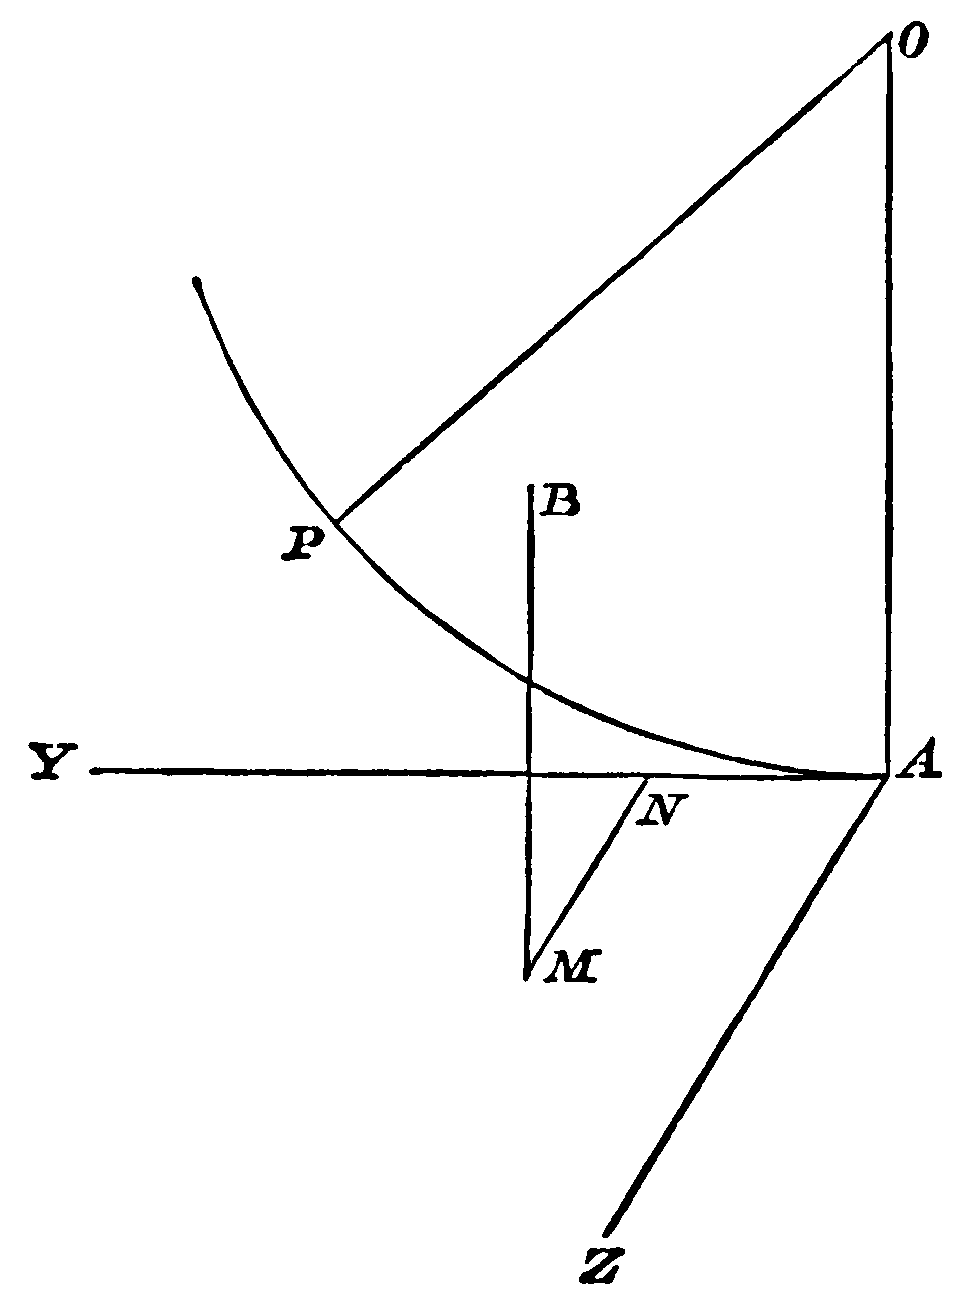
\includegraphics[width=0.46\textwidth]{290.png}
\centering
\end{figure}

Let \(A\) be the point \( (\mu, \varpi)\), so that \(POA = \theta\).

Take \(A\) as the origin of a new set of coordinates; let \(AO\) be
the axis of \(x\), \(AY\) the tangent to \(AP\) the axis of \(y\), and \(AZ\) which
is perpendicular to the plane of the paper the axis of \(z\). Then
the equation to the surface of the sphere will be
\[
2x = x^2 + y^2 + z^2. \tag{3}
\]

Transform to polar coordinates by the usual relations
\[
z = \rho \cos p, \quad x = \rho \sin p \cos q, \quad y = \rho \sin p \sin q.
\]

Then from (3) we obtain for the radius vector \(\rho\) the value
\[
\rho = 2 \sin p \cos q.
\]
%%-----File: 291.png-----%%

Now we know by the Integral Calculus that the polar expression
for an element of a surface is
\[
{\bigsurd} \left\{\rho^2 \sin^2 p + \sin^2 p \left(\frac{d\rho}{dp}\right)^2 + \left(\frac{d\rho}{dq}\right)^2\right\}\rho\, dp\, dq.
\]
In the present case this becomes \(2\rho \sin p\, dp\, dq\).

And we know that \(\xsurd(2 - 2\lambda)\) expresses the same thing as \(\rho\),
that is the distance between \((\mu, \varpi)\) and \((\mu', \varpi')\), that is the
distance between the new origin and \((\rho, p, q)\).

Hence, finally, \(\xxp\displaystyle\iint \xp\dfrac{Y' d\mu' d\varpi'}{\xsurd(2 - 2\lambda)}\) transforms to \(\xxp\displaystyle\iint \xp\dfrac{Y' 2\rho \sin p\, dp\, dq}{\rho}\),
that is to \(2 \xxp\displaystyle\iint Y' \sin p\, dp\, dq\).

And from the diagram we see that the limits of the integrations
are \(-\xp\dfrac{1}{2} \pi\) and \(\xp\dfrac{1}{2} \pi\) for \(q\), and \(0\) and \(\pi\) for \(p\).

\Section
1259. We have now to connect the old variables with
the new.

Let \(B\) denote the point \((\mu', \varpi')\) on the surface of the sphere,
that is the point \((\rho, p, q)\). Let \(M\) be the projection of \(B\) on the
plane of \((y, z)\), and \(N\) the projection of \(M\) on the axis of \(y\). The
straight lines \(AB\) and \(OB\) may be supposed to be drawn.

We shall project \(AB\) on \(OP\) in two ways, and equate the
results.

First consider \(AB\) as made up of the components \(AO\) and
\(OB\). Thus we get as the projection
\[
\cos \theta' - \cos \theta.
\]

Next consider \(AB\) as made up of the components \(AN\), \(NM\),
and \(MB\). Thus we get as the projection
\[
y \sin \theta - x \cos \theta.
\]
Therefore
\[
\cos \theta' - \cos \theta = y \sin \theta - x \cos \theta,
\]
so that
\[
\cos \theta' = (1 - x) \cos \theta + y \sin \theta.
\]
%%-----File: 292.png-----%%

Put for \(x\) and \(y\) their values in terms of \(p\) and \(q\); hence
we get
\[
\mu' = \mu \cos^2 p - \sin^2 p \cos(2q + \theta). \tag{4}
\]

Again \(\varpi' - \varpi\) is the angle between the planes \(POA\) and
\(POB\). Hence the perpendicular from \(B\) on the plane \(POA\) is
\(\sin\theta' \sin(\varpi'-\varpi)\); and this perpendicular is equal to \(MN\),
so that
\[
\sin\theta' \sin (\varpi' - \varpi) = z,
\]
that is
\[
\sin\theta' \sin(\varpi' - \varpi) = 2 \sin p \cos p \cos q. \tag{5}
\]

The equations (4) and (5) are theoretically sufficient to connect
the old variables with the new; but another equation will
also be useful in some cases, namely,
\[
\sin\theta' \cos(\varpi' - \varpi) = \sin\theta - y \cos\theta - x\sin\theta.
\]

This may be obtained thus: suppose \(B\) projected on the plane
\(POA\), let \(L\) denote the projection; so that \(L\) is in fact the point
\((x, y, 0)\). Then the equation just written may be obtained by
two ways of projecting \(OL\) on a straight line at right angles to
\(OP\); in one way \(OL\) is projected immediately, and in the other
way it is made up of the components \(OA\), \(AN\), and \(NL\).

The equation becomes by putting for \(x\) and \(y\) their values
\[
\sin\theta' \cos(\varpi' - \varpi) = \sin\theta - 2 \sin^2 p \cos q \sin(q + \theta). \tag{6}
\]

The equation (6) is not independent of (4) and (5); it will be
found that if we square and add (5) and (6) so as to eliminate
\(\varpi' - \varpi\) we obtain a result which is equivalent to (4).

\Section
1260. Laplace himself does not give equation (5) nor equation
(6); because he does not require them. He begins by assuming
that the figure of the solid required is to be one of revolution; and
afterwards gives a supplementary investigation for the case in
which the figure is not assumed to be one of revolution. Thus in
this part of his process \(Y'\) is a function of \(\mu'\) only; but it is
convenient for us here to take the most general supposition,
namely, that \(Y'\) is a function of \(\varpi'\) as well as \(\mu'\).

\Section
1261. In (4) put \(2q + \theta = q'\); thus
\[
\mu' = \mu \cos^2 p - \sin^2 p \cos q'. \tag{7}
\]
%%-----File: 293.png-----%%

Hence from the result of Art.\ 1258, we have
\[\int_{-1}^1 \int_{0}^{2\pi} \frac{Y' d\mu' d\varpi'}{\xsurd(2 - 2\lambda)} = \int_{0}^\pi \int_{-\pi+\theta}^{\pi+\theta} Y' \sin p\, dp\, dq'. \tag{8}\]

Thus it will be seen that (8) does not quite agree with (2)
because the limits of \(q'\) are not the same in the two formulæ.

If with Laplace we assume that \(Y'\) is a function of \(\mu'\) only,
then by substituting for \(\mu'\) by (7) we make \(Y'\) a function of \(p\) and
of \(q'\) such that \(q'\) enters through \(\cos q'\). In this case by the first
principles of the Integral Calculus the limits for \(q'\) may be any
that just comprise the range \(2\pi\), and so we may take them to be
0 and \(2\pi\). Hence if \(Y'\) is a function of \(\mu'\) only the formula (2) is
established.

But when \(Y'\) is a function of \(\varpi'\) as well as of \(\mu'\) it does not
seem to me that this passage from (8) to (2) can be always effected.
In this case we must express \(\varpi'\) in terms of the new variables by
(5) and (6). Hence we get by division
\[\varpi' - \varpi = \tan^{-1}\left\{\frac{2 \sin p \cos p \cos q}{\sin \theta - 2 \sin^2 p \cos q \sin (q + \theta)}\right\}\text{.}\]

Thus when we put \(q = \xp\dfrac{q'}{2} - \xp\dfrac{\theta}{2}\), we shall introduce \(\sin \xp\dfrac{q'}{2}\) and
\(\cos \xp\dfrac{q'}{2}\); and we cannot assert that the limits of the integration with
respect to \(q'\) can be changed from \(-\pi + \theta\) and \(\pi + \theta\) to 0 and \(2\pi\).

Although the truth of (2) is asserted by Liouville and admitted
by Poisson, even in the case in which \(Y'\) is a function of \(\varpi'\) as
well as \(\mu'\), yet for the reason just given the result seems to me
inadmissible. See pages 212 and 312 of the volume cited in
Art.\ 1255.

\Section
1262. Admitting then the truth of (2) on Laplace's supposition,
let us see how he applies it.

Let \(\kappa\) denote the centrifugal force at the distance unity from
the axis. Then for relative equilibrium we must have
\[V + \frac{a^2}{2} \kappa(1 - \mu^2) = \text{constant.}\]
%%-----File: 294.png-----%%

But from (1) and (2) we have
\[V = \frac{4\pi a^2}{3} (1 - \alpha Y) + a^2\alpha \int_{0}^{\pi} \int_{0}^{2\pi} Y'\sin p\,dp\,dq' \tag{9}.\]

Hence, dividing by \(a^2\), we get
\[\frac{4\pi}{3}\alpha Y - \alpha \int_{0}^{\pi} \int_{0}^{2\pi} Y' \sin p\,dp\,dq' - \frac{\kappa}{2} (1 - \mu^2) = C \tag{10},\]
where \(C\) is a constant.

Differentiate (10) three times with respect to \(\mu\), and observe
that by (7) we have \(\xp\dfrac{d\mu'}{d\mu} = \cos^2 p\). Thus
\[\frac{4\pi}{3} \frac{d^3Y}{d\mu^3} - \int_{0}^{\pi} \int_{0}^{2\pi} \frac{d^3Y'}{d\mu'^3} \sin p \cos^6 p\,dp\,dq' = 0,\]
that is
\[\int_{0}^{\pi} \int_{0}^{2\pi} \left( \frac{7}{3} \frac{d^3Y}{d\mu^3} - \frac{d^3Y'}{d\mu'^3}\right) \sin p \cos^6 p\,dp\,dq' = 0.\]

Laplace then says:
\begin{squote}
Cette équation doit avoir lieu, quel que soit \(\mu\); or il est clair que
parmi toutes les valeurs comprises depuis \(\mu = -1\), jusqu'à \(\mu = 1\), il en
existe une que nous désignerons par \(h\), et qui est telle, qu'abstraction
faite du signe, aucune des valeurs de \(\xp\dfrac{d^3Y}{d\mu^3}\) ne surpassera pas celle qui
est relative à \(h\); en désignant donc par \(H\), cette dernière valeur, on
aura
\[\int_{0}^{\pi} \int_{0}^{2\pi} \left( \frac{7}{3} H - \frac{d^3Y'}{d\mu'^3}\right) \sin p \cos^6 p\,dp\,dq' = 0.\]

La quantité \(\xp\dfrac{7}{3}H - \xp\dfrac{d^3Y'}{d\mu'^3}\) est évidemment du même signe que \(H\), et le
facteur \(\sin p\cos^6 p\) est constamment positif dans toute l'étendue de l'intégrale;
les élémens de cette intégrale sont donc tous du même signe que \(H\);
d'où il suit que l'intégrale entière ne peut être nulle, à moins que \(H\) ne le
soit lui-même, ce qui exige que l'on ait généralement, \(0 = \xp\dfrac{d^3Y}{d\mu^3}\), d'où l'on
tire en intégrant,
\[Y = l + m\mu + n\mu^2;\]
\(l\), \(m\), \(n\), étant des constantes arbitraires.
\end{squote}
%%-----File: 295.png-----%%

\Section
1263. This reasoning, says Liouville, is specious and might
at the first glance deceive us; but on reflecting we see that it
ceases to be applicable if the maximum of the function \(\xp\dfrac{d^3Y}{d\mu^3}\) could
be infinite; and this would be the case if for example \(Y = (1 - \mu^2)^{\frac{3}{2}}\)
or \((1 - \mu^2)^{\frac{7}{3}}\).

In order to manifest the unsoundness of the principle on
which this reasoning rests, Liouville takes a very simple example.
Suppose it required to find a function \(\phi(x)\) which satisfies the
equation
\[
\int_{0}^{1} \phi(\alpha x)\, d\alpha = \frac{3}{10} \phi(x), \tag{11}
\]
\(x\) being an independent variable.

Differentiate three times with respect to \(x\); thus
\[
\int_{0}^{1} \alpha^3 \phi'''(\alpha x)\, d\alpha = \frac{3}{10} \phi'''(x),
\]
or, which is the same thing,
\[
\int_{0}^{1} \alpha^3 \left\{ \frac{12}{10} \phi'''(x) - \phi'''(\alpha x)\right\} d\alpha = 0.
\]

Now if we apply to this equation and the function \(\phi(x)\) the
reasoning of Laplace, without changing a word, we shall arrive as
before at the result \(\phi'''(x) = 0\). But this is absurd, for the value
of \(\phi(x)\) which satisfies (11) is obviously of the form \(\phi(x) = Ax^{\frac{7}{3}}\),
where \(A\) is an arbitrary constant.

Similarly by putting the equation
\[
\int_{0}^{1} \phi(\alpha x)\, d\alpha = 2\phi(x) \tag{12}
\]
in the form
\[
\int_{0}^{1} \{2\phi(x) - \phi(\alpha x)\}\, d\alpha = 0,
\]
we might conclude by Laplace's reasoning that \(\phi(x) = 0\). But it
is obvious that (12) is satisfied by the more general value
\[
\phi(x) = \frac{A}{\xsurd x}.
\]
%%-----File: 296.png-----%%

Thus in order that Laplace's demonstration should be sufficient
it would be necessary to shew that \(\xp\dfrac{d^3Y}{d\mu^3}\) is always finite. But
this would amount to imposing additional restriction on the
value of \(Y\), when the only restriction that ought to be used is
that \(Y\) is to be always finite. Therefore some method must be
employed very different from Laplace's.

\Section
1264. Accordingly Liouville gives another demonstration;
it is rather long, but interesting and satisfactory.

He restricts himself to the case in which the figure is assumed
to be one of revolution; for the remainder of the problem he refers
to the supplementary investigation which, as I have stated in
Art.\ 1260, Laplace himself gave.

As I have stated in Art.\ 1261, Liouville asserts the universal
truth of (2); yet he confines himself, as Laplace did, to the case
in which \(Y'\) is a function of \(\mu'\) only; and thus his process is not
affected by my objection to the universal truth of (2).

The process used by Liouville does not admit of any convenient
abbreviation; and I must therefore leave the student to
consult the original paper.

\Section
1265. I now pass to a paper by Poisson, which is entitled
\textit{Note relative à un passage de la Mécanique céleste}; it is given in
Liouville's \textit{Journal de Mathématiques}, Vol.\ \textsc{ii}.\ 1837, pages 312\dots 316.
I shall translate this paper, for the investigation which it contains
is so brief and simple, that it ought to form part of any standard
treatise on the subject.

In the translation, I shall continue the numbering of the
equations which has been already used in the Chapter.

\Section
1266. In the twenty-sixth section of the Third Book [of the
\textit{Mécanique Céleste}] the author proposes to demonstrate, without
recourse to the reduction into a series, that a homogeneous fluid
turning uniformly round a fixed axis has only a single figure of
equilibrium which differs very little from a sphere. The objection
which M. Liouville has urged against the generality of this demonstration
is real; see the number of this \textit{Journal} for the month of
%%-----File: 297.png-----%%
June last: but the demonstration which he has substituted for that
of the \textit{Mécanique Céleste} is very complicated, and we may arrive
more simply at the result by the following considerations which
differ less from those which Laplace used.

I retain without stating it here, all the notation of the memoir
of M. Liouville, and the equation (10) cited at the beginning of
the second article, that is
\[
C = \frac{4\pi \alpha}{3} Y - \alpha \int_0^\pi \int_0^{2\pi} Y'
\sin p \,dp \,dq' -\frac{1}{2} \kappa(1 - \mu^2). \tag{10}
\]

The radius vector \(r\) of any point of the surface is represented
by
\[
r = a (1 + \alpha Y).
\]

The unknown quantity \(Y\) may be any function of the two
variables denoted by \(\mu\) and \(\varpi\), provided it is always finite. We
do not assume that the surface is one of revolution, or that \(Y\)
is independent of the angle \(\varpi\); nor do we assume that the fluid
has its centre of gravity on the axis of rotation: we assume only
that the figure differs very little from a sphere which would have
its centre on this axis. The constant \(a\) may differ from the
radius of the sphere equivalent in volume to the fluid, provided
that the difference is of the order of smallness of \(\alpha\), the same as that
of \(\kappa\), and the square of which we neglect.

The rigorous condition of equilibrium consists in this, that the
sum of the elements of the fluid divided by their respective
distances from any point of the surface, together with the quantity
\(\xp\dfrac{1}{2} a^2 \kappa(1 -\mu^2)\), which arises from the centrifugal force at the point,
should be constant. The part of this constant relative to the
sphere of radius \(a\) and independent of the centrifugal force, is
equal to \(\xp\dfrac{4\pi a^2}{3}\); the part relative to this force and to the non-sphericity
of the fluid is \(-a^2 C\), where \(C\) is the constant of the
preceding equation. If we denote by \(\gamma\) its complete value
we have
\[
\gamma = \frac{4\pi a^2}{3} - a^2 C.
\]
%%-----File: 298.png-----%%

Now for each possible figure of equilibrium this constant \(\gamma\) is
evidently a determinate quantity, which cannot depend on the
radius that we take for \(a\), that is to say, on the difference between
this radius and that of the sphere which is equivalent to the
given volume of the fluid. The constant \(C\) then is indeterminate
like this difference; so that for any value we may take for \(a\), the
preceding equation will determine the corresponding value of \(C\);
and conversely, if we take for \(C\) a value which is of the order of
smallness of \(\alpha\), this equation will determine the radius \(a\).

Suppose then
\[
Y = l\mu+ m\mu^2 + X,
\]
\(l\) and \(m\) being undetermined constants, and \(X\) a new unknown
function of \(\mu\) and \(\varpi\), the values of which are always finite. Let \(c\)
denote the greatest of these values, and put
\[
c-X=Z;
\]
then the unknown quantity \(Z\) can never be negative, and the
expression for \(Y\) will become
\[
Y = c + l\mu + m\mu^2 - Z.
\]

Substitute this in the equation (10). Let \(\mu'\) denote what \(\mu\)
becomes in \(Y'\), then
\[
\mu' = \mu \cos^2 p - \sin^2 p \cos q'.
\]

Hence we shall have
\[\begin{aligned}
\int_0^\pi \int_0^{2\pi} \mu' \sin p \,dp \,dq' &= \frac{4\pi\mu}{3},\\
\int_0^{\pi} \int_0^{2\pi} \mu'^2 \sin p \,dp \,dq' &= \frac{4\pi}{5} (\mu^2 + \frac{4}{3});
\end{aligned}\]
and also we have
\[
\int_0^\pi \int_0^{2\pi} \sin p \,dp \,dq' = 4\pi.
\]

The result of the substitution then will be
\begin{gather*}
C = \left(\frac{8\pi\alpha}{15} m + \frac{1}{2} \kappa\right)\mu^2 - \frac{16\pi\alpha}{15} m - \frac{8\pi\alpha}{3} c - \frac{1}{2} \kappa\\
- \frac{4\pi\alpha}{3} Z + \alpha \int_0^\pi \int_0^{2\pi} Z' \sin p \,dp \,dq',
\end{gather*}
%%-----File: 299.png-----%%
where \(Z'\) denotes what \(Z\) becomes in \(Y'\).

Now since the constants \(m\) and \(C\) can be taken arbitrarily,
we may suppose that
\[\frac{8\pi \alpha}{15} m + \frac{1}{2} \kappa = 0,\]
\[C = -\frac{16\pi \alpha}{15} m - \frac{8\pi \alpha}{3} c - \frac{1}{2} \kappa\tag{13},\]
which reduces the preceding equation to
\[\int_0^\pi \int_0^{2\pi} Z' \sin p\, dp\, dq' - \frac{4\pi}{3} Z = 0,\]
which may be written in this form,
\[\int_0^\pi \int_0^{2\pi}\left(Z' - \frac{1}{3} Z\right) \sin p\, dp\, dq' = 0.\]

Now let \(h\) and \(k\) denote the values of \(\mu\) and \(\varpi\), which correspond
to the least of all the possible values of \(Z\); and denote by
\(L\) the least value; for \(\mu = h\), and \(\varpi = k\), the last equation will
become
\[\int_0^\pi \int_0^{2\pi}\left(Z' - \frac{1}{3} L\right)\sin p\, dp\, dq' = 0 \tag{14}.\]

But it is evident that \(Z'\) or \(Z\) being by hypothesis a positive
quantity or zero, the difference \(Z' - \xp\dfrac{1}{3} L\) is also positive or zero.
Then as all the elements of the double integral have the same
sign the double integral cannot be zero unless the factor \(Z' - \xp\dfrac{1}{3} L\)
is zero; and this condition cannot be satisfied unless \(Z'\) or \(Z\) is
constantly zero.

From the preceding equations we obtain
\[\begin{aligned}m &= -\frac{15\kappa}{16\pi \alpha},\\
c &= \frac{3\kappa}{16\pi \alpha}-\frac{3}{8\pi \alpha} C.\end{aligned}\]
%%-----File: 300.png-----%%

Substitute the values of \(m\) and \(c\) in the expression for \(Y\), suppressing
the term \(Z\); and put this expression in the value of \(r\):
thus
\[
r = a \left\{1 + \frac{3(\kappa - 2C)}{16\pi} + \alpha l \mu - \frac{15\kappa}{16\pi}\mu^2\right\}.
\]

This result involves the indeterminate constant \(\alpha l\), which
depends on the origin of the coordinates on the axis of rotation.
We may make it disappear by a convenient displacement of this
origin on this straight line; or if we please we may suppose it
zero, and write
\[
r= a\left\{1 + \frac{3(\kappa - 2C)}{16\pi} - \frac{15\kappa}{16\pi}\mu^2\right\}.
\]

We can also without difficulty make the constants \(a\) and \(C\)
disappear from the value of \(r\). In fact let
\[
a\left\{1 + \frac{3(\kappa - 2C)}{16\pi}\right\} = b\left(1 + \frac{5\kappa}{16\pi}\right) \tag{15};
\]
then neglecting the squares and the product of \(\kappa\) and \(C\), and
putting for brevity,
\[
\frac{15\kappa}{16\pi} = n,
\]
we shall have finally
\[
r = b\left\{1 + n\left(\frac{1}{3} - \mu^2\right)\right\}.
\]

It is easy to see from this expression for \(r\) that \(b\) is the radius
of the sphere equivalent in volume to the fluid, and so is given.
Thus there is nothing unknown or indeterminate in this expression,
and we conclude that the fluid has only one possible figure of
relative equilibrium which differs but little from a sphere: which
was to be proved.

This demonstration is more simple than that which is based
on the reduction of \(r\) to a series of a certain form, and which
supposes the properties of the terms of this development to be
known, as well as the generality of this form of series which had
been contested, but which I have placed beyond question in my
memoir on the \textit{Attraction of Spheroids} in the \textit{Additions à la
Connaissance des Tems}, 1829.
%%-----File: 301.png-----%%

If we put
\[a = b,\qquad aY = n \left(\frac{1}{3} - \mu^2\right),\]
in the expression \(a(1 + \alpha Y)\) for \(r\), which makes it coincide with
the final expression for the radius vector; and denote by \(B\) the
value of the constant \(C\), which corresponds to these values of \(a\)
and of \(\alpha Y\); and have regard to what \(n\) represents, we shall find
without difficulty that the equation (10) reduces to
\[B = -\frac{ 1}{3} \kappa.\]

We shall have at the same time
\[\gamma = \frac{4\pi b^2}{3} + \frac{1}{3} \kappa b^2.\]

As we have said above, this quantity \(\gamma\) ought to be the same
whatever radius, differing little from \(b\), we take for \(a\); thus we
must have
\[\frac{4\pi b^2}{3} + \frac{1}{3} \kappa b^2 = \frac{4\pi a^2}{3} - a^2 C.\]

This result coincides in fact with equation (15), neglecting
always the squares and the product of \(\kappa\) and \(C\).

\Section
1267. Such is Poisson's treatment of the problem: I shall
make two remarks on it.

In the first place it will be seen that Poisson assumes the
truth of equation (2), which I do not allow. But on examination
it will be found that equation (8), which has been strictly demonstrated,
will be sufficient for his purpose; so that no objection
can be taken on this ground to the demonstration.

Secondly, the quantity which Poisson designates by \(L\) is
simply zero; for he assumes \(c\) to be the greatest value of \(X\),
and so when \(X\) is equal to \(c\), the value of \(Z\) is least, namely zero.

\Section
1268. I venture to propose the following demonstration,
which though less decisive than Poisson's may be found worthy of
study.

Let us restrict ourselves to the case of figures of revolution.
Then take the equation which has been already established,
\[\frac{4\pi \alpha}{3} Y - \alpha \int_{0}^{\pi} \int_{0}^{2\pi} Y' \sin p\, dp\, dq' - \frac{\kappa}{ 2} (1 - \mu^2) = \text{constant.}\]
%%-----File: 302.png-----%%

Assume
\[Y = - \frac{15\kappa}{16\alpha\pi} \mu^2 + Z;\]
thus we obtain
\[\frac{4\pi \alpha}{3} Z - \alpha \int_{0}^{\pi} \int_{0}^{2\pi} Z' \sin p\, dp\, dq' = \text{constant.}\tag{16}\]

Differentiate with respect to \(\mu\); thus
\[\frac{4\pi}{3}\frac{dZ}{d\mu} - \int_{0}^{\pi}\int_{0}^{2\pi} \frac{dZ'}{d\mu'} \cos^2 p \sin p\, dp\, dq' = 0,\]
which may be written
\[\int_{0}^{\pi} \int_{0}^{2\pi} \left(\frac{dZ}{d\mu} - \frac{dZ'}{d\mu'}\right)\cos^2 p \sin p\, dp\, dq' = 0.\]

But this is impossible unless \(\xp\dfrac{dZ}{d\mu}\) is a constant. For if \(\xp\dfrac{dZ}{ d\mu}\) be
not constant take \(\theta\) so that \(\xp\dfrac{dZ}{d\mu}\) has its greatest value, then
\(\xp\dfrac{dZ}{d\mu} - \xp\dfrac{dZ'}{d\mu'}\) is never negative; and the definite double integral
must have some positive value, and not be zero. Hence \(\xp\dfrac{dZ}{d\mu}\) must
be a constant; so that \(Z = l\mu + h\), where \(l\) and \(h\) are constant.

This shews that for surfaces of revolution the figure must be
that of an oblatum, which becomes a sphere if \(\kappa = 0\).

Then by Laplace's supplementary investigation the solution of
the problem may be extended to the case in which the figure is
not assumed to be one of revolution.

It may be objected to the above process that it is not quite
satisfactory, for \(\xp\dfrac{dZ}{d\mu}\) might be infinite. It would I think be a
sufficient answer to say that if \(\xp\dfrac{dZ}{d\mu}\) can be infinite then \(\xp\dfrac{dr}{d\mu}\)
will be infinite; and there would be a singular line on the
surface of the nature of a ridge or chasm, or a mountain or valley
with vertical sides; but it might be shewn by general reasoning
that in such cases there would not be relative equilibrium. Moreover
the approximate value of \(V\) which we have used throughout
%%-----File: 303.png-----%%
cannot be held to be safely established unless we admit that
\(\xp\dfrac{dr}{d\mu}\) is never infinite.

\Section
1269. But it may I think be shewn that a value of \(\phi(\mu)\)
which itself always remains finite, but allows \(\xp\dfrac{d\phi(\mu)}{d\mu}\) to be infinite,
cannot satisfy the equation
\[\frac{4\pi}{3}\phi(\mu) = \int_0^{2\pi} \int_0^\pi \phi(\mu\cos^2 p - \sin^2 p \cos q)\sin p\, dq\, dp + C \tag{17},\]
where \(C\) is a finite constant. This equation is equivalent to (16).

Let \(\mu_1\) and \(\mu_2\) be particular values of \(\mu\); put \(u\) for
\[\frac{\phi(\mu_2) - \phi(\mu_1)}{\mu_2 - \mu_1},\]
and \(v\) for
\[\frac{\phi(\mu_2\cos^2 p - \sin^2 p \cos q) - \phi(\mu_1\cos^2 p - \sin^2 p\cos q)}{\mu_2 - \mu_1},\]
then we deduce from (17)
\[\frac{4\pi}{3}u = \int_0^{2\pi} \int_0^\pi v\sin p\, dq\, dp\tag{18},\]
and this is true however small \(\mu_2 - \mu_1\) may be.

Now I say that if \(\xp\dfrac{d\phi(\mu)}{d\mu}\) could be infinite, we could make the
left-hand member of (18) incomparably greater than the right-hand
member; which is absurd.

For suppose \(\mu_1\) to denote the value of \(\mu\) for which \(\xp\dfrac{d\phi(\mu)}{d\mu}\)
becomes infinite; then we can make \(u\) as large as we please,
by taking \(\mu_2 - \mu_1\) small enough. But \(v\) will be very large indeed
only over a very small part of the range of integration; in fact
an infinitesimal part. However let \(\sigma\) denote a small but finite
part of the whole spherical surface, over which the integration
with respect to \(v\) may be supposed to extend, namely, that part
within which the very large values of \(v\) occur. Then \(v\) will be
numerically less than \(u\), except \(p\) should happen to be zero.
Thus the corresponding part of the right-hand member of (18)
may be denoted by \(\lambda u\sigma\) where \(\lambda\) denotes some proper fraction.
%%-----File: 304.png-----%%
The rest of (18) may be denoted by \((4\pi - \sigma)w\), where \(w\) denotes
some value of \(v\) intermediate between the greatest and least of
a set of values which are all finite.

Thus instead of (18) we have
\[\frac{4\pi}{3} u = \lambda u \sigma + (4\pi - \sigma)w\tag{19}.\]

We can of course take \(\sigma\) far less than \(\xp\dfrac{4\pi}{3}\); and then as \(u\)
increases indefinitely, the left-hand member of (19) is obviously far
greater than the right-hand.

The same reasoning holds if we suppose that \(\xp\dfrac{d\phi(\mu)}{d\mu}\) can become
infinite, twice, or thrice, or any finite number of times.

The argument may be much strengthened by observing that
\(v\) when very large is not always of the same sign; it may be said
roughly to be as often positive as negative. This \textit{attenuates} extremely
the values of \(\lambda\) in (19).

\Section
1270. We may now conveniently introduce Laplace's supplementary
investigation to which we have alluded in Art.\ 1260.
We have already arrived at the following result: if a fluid mass
in the form of a figure of revolution, nearly spherical, rotating
with uniform angular velocity is in relative equilibrium, the form
must be that of an oblatum; and if there is no rotation the oblatum
reduces to a sphere. The result is then to be extended to
the case where the figure is not assumed to be one of revolution.

\Section
1271. Return to equation (10) corrected as in (8). Suppose
that besides the value \(a(1 + \alpha Y')\) which belongs to an oblatum,
the equation may be satisfied by another value of the radius
vector which we will denote by \(a(1 + \alpha Y' + \alpha v')\), where \(v'\) is some
function of \(\theta'\) and \(\varpi'\). Thus
\[\frac{4\pi \alpha Y}{3} - \alpha \int_0^\pi \int_{-\pi+\theta}^{\pi+\theta} Y' \sin p\, dp\, dq' - N = \text{constant,}\]
where \(N\) is the expression arising, as in Art.\ 1262, from the centrifugal
force, or other small given external forces.
%%-----File: 305.png-----%%

Also
\[\frac{4\pi\alpha}{3}(Y + v) - \alpha\int_{0}^{\pi} \int_{-\pi + \theta}^{\pi+\theta} (Y' + v') \sin p\,dp\,dq' - N = \text{constant.}\]

Hence, by subtraction,
\[\frac{4\pi \alpha v}{3} - \int_{0}^{\pi} \int_{-\pi+\theta}^{\pi + \theta} v' \sin p\,dp\,dq' = \text{constant.} \tag{20}\]

Laplace himself does not state what the limits of the integration
for \(q'\) are; I give them in accordance with my remarks in
Art.\ 1261.

The equation (20) is obviously that of a homogeneous spheroid
in equilibrium, of which the radius vector is \(a(1 + \alpha v)\), and in
which there is no force acting besides the attractions of the molecules.
Now as the equation is satisfied whatever be the value
of \(\varpi\) by the radius vector \({a(1 + \alpha v})\), we may in this radius vector
change \(\varpi\) successively into \({\varpi + d\varpi}\), \(\varpi + 2d\varpi\), \dots. Denote by
\(v_{1}\), \(v_{2}\), \dots\ what \(v\) becomes by reason of these successive changes.
Then the equation will also be satisfied by the radius vector
\[a\{1 + \alpha v_{1} d\varpi + \alpha v_{2} d\varpi + \alpha v_{3} d\varpi + \ldots\}\text{.}\]

Hence we may take for the radius vector \(a(1 + \alpha\mystrut(0,3) \displaystyle\int_{0}^{2\pi} v d\varpi)\),
which will be the radius vector of a surface of revolution. Now
as we have shewn in Art.\ 1268, this must be the surface of a sphere.
Let us see what \(v\) must consequently be.

Let \(a\) be the shortest distance of the centre of gravity of the
spheroid of which the radius vector is \(a(1 + \alpha v)\) from the surface;
and let us place the pole, that is the origin of the angle \(\theta\), at the
extremity of the shortest distance. Then \(v\) will be zero at the
pole, and positive at every other place; and the same will be true
for \(\xxp\displaystyle\int_{0}^{2\pi} v d\varpi\). Now as the centre of gravity of the spheroid which
has the radius vector \({a(1 + \alpha v)}\) is at the centre of the sphere of
radius \(a\), so also is the centre of gravity of the spheroid of which
the radius vector is \(a(1 + \alpha\xxp\displaystyle\int_{0}^{2\pi} v d\varpi)\). The radii vectores drawn
from the centre to the surface of the last spheroid are therefore
%%-----File: 306.png-----%%
unequal if \(v\) is not zero; and so the surface cannot be that of a
sphere, unless \(v\) is zero. Hence we are certain that a homogeneous
fluid which is acted on by very small external forces,
and is nearly spherical, can be in equilibrium in only one way.

I may observe that there is an awkward note on Bowditch's
page 275, numbered 1183. To make his process sound, instead
of \(a (1 + \alpha \xxp\displaystyle\int_0^{2\pi} vd\varpi)\) for the radius he should use \(a\xxp\left(1 + \dfrac{\alpha}{2\pi} \displaystyle\int_0^{2\pi} vd\varpi\right)\).

\Section
1272. Another paper on the subject is given in the fourth
volume of the \textit{Journal de Mathématiques} 1839. This is entitled
\textit{Extrait d'une Lettre de M. Wantzel à M. Liouville}; it occupies
pages 185\dots 188 of the volume.

The paper commences thus:
\begin{squote}
Je me suis occupé de nouveau de la question d'Analyse qui a pour
but de déterminer la figure d'équilibre d'une masse fluide soumise aux
attractions de ses particules et animée d'une vitesse constante de rotation,
lorsqu'on suppose cette figure peu différente de la sphère. Je crois
avoir levé l'objection que vous avez faite à la seconde méthode de Laplace
dans le tome \textsc{ii}.\ du \textit{Journal de Mathématiques} (juin 1837), ou plutôt
avoir rendu cette méthode rigoureuse par une légère modification.
\end{squote}

Wantzel's paper is not very clear, and it does not seem to me
satisfactory. He introduces into some of the expressions a variable
factor which is ultimately equal to unity; but the step seems to
me not justified. The paper is not of sufficient interest to warrant
me in devoting more space to it.

\Section
1273. It may be useful to give the process by which equation
(8) can be obtained from the ordinary formulæ for the transformation
of double integrals.

Take the two equations
\begin{gather*}
\mu' - \mu \cos^2 p + \sin^2 p \cos(2q + \theta) = 0,\\
\xsurd(1 - \mu'^2) \sin(\varpi' - \varpi) - 2 \sin p \cos p \cos q = 0;
\end{gather*}
denote the former by \(F_1 = 0\), and the latter by \(F_2 = 0\).
%%-----File: 307.png-----%%

Then we know that the transformations consist in replacing
\(d\mu' \,d\varpi'\) by
\[
\frac{\dfrac{dF_1}{dp} \dfrac{dF_2}{dq} - \dfrac{dF_1}{dq} \dfrac{dF_2}{dp}}
{\dfrac{dF_1}{d\mu'} \dfrac{dF_2}{d\varpi'} - \dfrac{dF_1}{d\varpi'} \dfrac{dF_2}{d\mu'}}\, dp \,dq.
\]

Now
\[\begin{aligned}
\frac{dF_1}{dp} &= \sin 2p\{\cos(2q+\theta)+\mu\},\\
\frac{dF_2}{dq} &= \sin 2p\sin q,\\
\frac{dF_1}{dq} &= -2\sin^2 p\sin(2q+\theta),\\
\frac{dF_2}{dp} &= -2\cos 2p\cos q;\\
\end{aligned}\]
therefore
\begin{gather*}
\frac{dF_1}{dp} \frac{dF_2}{dq} - \frac{dF_1}{dq} \frac{dF_2}{dp}\\
=\sin^2 2p\sin q\{\cos(2q+\theta)+\mu\} - 4\sin^2 p\cos 2p\cos q\sin(2q+\theta).
\end{gather*}

In this, the term involving \(\cos \theta\)
\[\begin{aligned}
&= 4\sin^2 p\{(1+\cos 2q)\sin q\cos^2 p -\cos 2p\cos q\sin 2q\}\cos \theta\\
&= 8\sin^2 p\cos ^2 q\sin q(\cos^2 p -\cos 2p)\cos \theta\\
&= 8\sin^4 p\cos^2 q\sin q\cos \theta\\
&= 2 \rho^2\sin^2 p\sin q\cos \theta.
\end{aligned}\]

The term involving \(\sin \theta\)
\[\begin{aligned}
&= -4\sin^2 p\{\cos^2 p\sin q\sin 2q +\cos 2p\cos q\cos 2q\}\sin \theta\\
&= -4\sin^2 p\{\cos^2 p\cos q -\sin^2 p\cos q\cos 2q\}\sin \theta\\
&= -4\sin^2 p\cos q\sin \theta + 8\sin^4 p\cos^3 q\sin \theta\\
&= -2\rho\sin p\sin \theta + 2 \rho^2\sin^2 p\cos q\sin \theta.
\end{aligned}\]

Thus
\begin{gather*}
\frac{dF_1}{dp} \frac{dF_2}{dq} - \frac{dF_1}{dq} \frac{dF_2}{dp}
= -2\rho\sin p\{\sin \theta - \rho\sin p\sin (q+\theta)\}\\
= -2\rho\sin p\sin \theta'\cos (\varpi' - \varpi) \text{ by equation (6).}
\end{gather*}
%%-----File: 308.png-----%%

And
\[\frac{dF_1}{d\mu'}\frac{dF_2}{d\varpi'} - \frac{dF_1}{d\varpi'}\frac{dF_2}{d\mu'} = \xsurd(1 - \mu'^2)\cos(\varpi'-\varpi).\]

Hence \(d\mu'\, d\varpi'\) transforms to
\[\frac{-2\rho \sin p \sin\theta' \cos(\varpi' - \varpi)}{\xsurd(1 - \mu'^2)\cos(\varpi'-\varpi)} dp\, dq,\]
that is to
\[-2\rho \sin p\, dp\, dq.\]

And as \(\xsurd(2 - 2\lambda) = \rho\) it follows that
\[\frac{d\mu' d\varpi'}{\xsurd(2 - 2\lambda)}\text{ transforms to } \frac{-2\rho \sin p\, dp\, dq}{\rho},\]
that is to
\[-2\sin p\, dp\, dq.\]
%%-----File: 309.png-----%%

\Chapter{CHAPTER XXXIII.}
\Subhead{LAPLACE'S MEMOIRS.}
\Runhead{\textsc{laplace's memoirs.}}

\Section
1274. \textsc{Laplace} published various memoirs during the first
quarter of the present century. We shall here give a brief
notice of them, reserving a fuller account for the next Chapter,
which will be devoted to the fifth volume of the \textit{Mécanique Céleste},
where most of the investigations are reproduced.

\Section
1275. A paper entitled \textit{Sur l'anneau de Saturne} occurs on
pages 450\dots 453 of the \textit{Connaissance des Tems} for 1811, which
was published in 1809. The paper occurs also on pages 426\dots 428
of the \textit{Nouveau Bulletin \dots\ par la Société Philomatique}, Vol.\ \textsc{i}.\ 1807.

Laplace adverts to the results which he had obtained in the
third Book of the \textit{Mécanique Céleste} as to Saturn's ring. He
says that the fact of the rotation of the ring in about ten hours
and a half had been suggested by himself from theory and confirmed
by Herschel's observations. But some observations by
Schroeter seemed to throw doubt on the fact of the rotation.
Laplace makes some remarks with a view of explaining the discrepancy;
that is, he accounts for Schroeter's phenomena without
giving up the rotation.

Laplace gives some account of the labours of astronomers and
mathematicians on Saturn's ring in the \textit{Mécanique Céleste}, Vol.\ \textsc{v}.\
pages 288\dots 291. He says nothing about Schroeter in these pages.

\Section
1276. A paper entitled \textit{Sur la Rotation de la Terre} occurs on
pages 53\dots 60 of the \textit{Annales de Chimie \dots} Vol.\ \textsc{viii.}, published in
1818. It is said to have been read to the Academy of Sciences
on the 18th of May, 1818.
%%-----File: 310.png-----%%

This paper constituted the preamble to a memoir with the
same title printed in the \textit{Connaissance des Tems} for 1821; it is
entirely reproduced there.

\Section
1277. A paper entitled \textit{Sur la Figure de la Terre, et la Loi
de la pesanteur à sa surface}, occurs on pages 313\dots 318 of the
same volume of the \textit{Annales de Chimie}\dots. It is said to have been
read to the Academy of Sciences on the 3rd of August, 1818.

The paper is also printed on pages 122\dots 125 of the \textit{Bulletin \dots\
par la Société Philomatique} for 1818. This seems to have been
the preamble to the memoir which we shall notice in Art.\ 1286,
and which was reproduced in the second Chapter of the Eleventh
Book of the \textit{Mécanique Céleste}. The preamble is not however
reproduced with the memoir, though much of it is in the
pages 11\dots 16 of the first Chapter of the Eleventh Book of the
\textit{Mécanique Céleste}. Still there are some remarks in this paper
which do not reappear in the \textit{Mécanique Céleste}. For instance,
take the following sentence:
\begin{squote}
Dans le nombre infini des figures que comprend l'expression analytique
des surfaces de la mer et du sphéroïde terrestre, on peut en
choisir une qui représente l'élévation et les contours des continens et
des îles: ainsi, je trouve qu'un petit terme du troisième ordre, ajouté
à la partie elliptique du rayon terrestre, suffit pour rendre conformément
à ce que l'observation semble indiquer, la mer plus profonde et plus
étendue vers le pôle austral que vers le pôle boréal, et même pour laisser
ce dernier pôle à découvert.
\end{squote}

There is nothing about this matter in the memoir.

\Section
1278. A memoir entitled \textit{Sur la rotation de la Terre} occurs
on pages 242\dots 259 of the \textit{Connaissance des Tems} for 1821, which
was published in 1819. About half this memoir concerns us; the
rest relates to the movement of the plane of the Earth's equator
and to the movement of the plane of the Moon's orbit.

\Section
1279. The following interesting paragraph forms part of the
preamble:
\begin{squote}
Le système du sphéroïde terrestre et des fluides qui le recouvrent, est
troublé par les actions du Soleil et de la Lune, qui changent continuellement
%%-----File: 311.png-----%%
la position de son équateur. L'explication de ce changement
observé sous les noms de \textit{précession} et de \textit{nutation} est, à mon sens, le
résultat le plus frappant et le moins attendu de la découverte de la
pesanteur universelle. Les anciens avaient bien connu que la cause
du flux et du reflux de la mer réside dans ces deux astres. Képler avait
conclu de ce phénomène et des lois des mouvemens célestes, l'attraction
mutuelle de toutes les parties de la matière. Mais personne, avant
Newton, n'avait soupçonné la cause de la précession des équinoxes, cause
d'autant plus cachée, qu'elle dépend de l'aplatissement de la Terre,
inconnu jusqu'alors. La manière dont ce grand géomètre a déduit la
précession, de l'ellipticité du sphéroïde terrestre et de la théorie du mouvement
rétrograde des nœuds de l'orbe lunaire, deux choses qu'il avait
tirées de sa découverte; cette manière, dis-je, quoiqu'inexacte à plusieurs
égards, est un des plus beaux traits de son génie.
\end{squote}

\Section
1280. The part of the memoir with which we are concerned
contains results which are reproduced in the fifth Volume of the
\textit{Mécanique Céleste}: see the pages 16, 17 and 57\dots 67.

The mathematical investigation however is much simpler in
the memoir than in the \textit{Mécanique Céleste}; but I think not less
satisfactory.

\Section
1281. Laplace establishes the following theorem: Suppose
the density of every stratum of the Earth to be diminished by
the density of the sea; take one of the principal axes of this
imaginary spheroid passing through its centre of gravity; let
the Earth be supposed to rotate uniformly round this axis; then
supposing the sea to be in relative equilibrium, this axis will be
a principal axis of the whole mass of the Earth and sea, and the
centre of gravity of the imaginary spheroid will also be the centre
of gravity of the whole mass. The sea is assumed to cover the
whole surface of the Earth.

We will now give the mathematical investigation.

\Section
1282. Take the principal axis of the imaginary spheroid for
the axis of rotation. Let \(V\) denote the potential of the Earth,
and \(V'\) that of the sea at a point on the surface of the sea, which
has for polar coordinates the usual \(r\) and \(\mu\). Let \(\omega\) be the angular
velocity of rotation.
%%-----File: 312.png-----%%

Then for relative equilibrium we must have
\[
V + V' + \frac{\omega^2 r^2}{2} (1 - \mu^2) = \text{ constant.} \tag{1}
\]

Let the radius vector of any stratum of the Earth be \(a(1 + \alpha y)\),
and suppose that the density \(\rho\) is a function of \(a\). Let \(y\) be
expanded in a series of Laplace's functions denoted by
\[
Y_{1} + Y_{2} + Y_{3} + \ldots
\]

Let \(M\) denote the mass of the Earth. Then
\[
V = \frac{M}{r} + \frac{4\alpha\pi}{r} \int_{0}^{\mathrm{a}} \rho \frac{d}{da}\left\{\frac{a^4 Y_{1}}{3r} + \frac{a^5 Y_{2}}{5r^2} + \frac{a^6 Y_{3}}{7r^3} + \ldots \right\}da,
\]
where the upper limit of the integral denotes the value of \(a\) at the
surface of the solid part.

Suppose \(\sigma\) the density of the sea, and let the radius vector of
the surface of the sea be denoted by \(b(1 + \alpha z)\); and suppose
\(z\) expanded in a series of Laplace's coefficients \(Z_{1} + Z_{2} + Z_{3} + \ldots\)
Let \(\overline{y}\) denote the value of \(y\) at the surface of the solid part.
Then \(V'\) may be found by considering the sea to be the difference
between two homogeneous spheroids of density \(\sigma\), one having
for radius vector \(b(1 + \alpha z)\), and the other having for radius vector
\(\mathrm{a} (1 + \alpha \overline{y})\).

Thus if \(M'\) denote the mass of the sea
\[
V' = \frac{M'}{r} + \frac{4\alpha\pi\sigma}{r} \left\{ \frac{b^4 Z_{1} - \mathrm{a}^4 \overline{Y}_1}{ 3r} + \frac{b^5 Z_{2} - \mathrm{a}^5 \overline{Y}_2}{5r^2} + \ldots \right\}.
\]

Hence (1) may be expressed thus:
\begin{gather*}
\frac{M + M'}{r} + \frac{4\alpha\pi}{r} \int_{0}^\mathrm{a} (\rho - \sigma) \frac{d}{da} \left\{ \frac{a^4 Y_{1}}{3r} + \frac{a^5 Y_{2}}{5r^2} + \frac{a^6 Y_{3}}{7r^3} + \ldots \right\}da\\
+ \frac{4\alpha\pi\sigma}{r} \left\{\frac{b^4 Z_{1}}{3r} + \frac{b^5 Z_{2}}{5r^2} + \frac{b^6 Z_{3}}{7r^3} + \ldots \right\}\\
- \frac{\omega^2 r^2}{2} (\mu^2 - 1) = \text{constant.}
\end{gather*}
%%-----File: 313.png-----%%

Then approximate, rejecting \(\alpha^2\); thus
\begin{align*}
&-\frac{M + M'}{b}\alpha\{Z_{1} + Z_{2} + Z_{3} + \ldots\}\\
&\qquad +\frac{4\alpha\pi}{b}\int_{0}^\mathrm{a} (\rho - \sigma) \frac{d}{da}\left\{\frac{a^4 Y_{1}}{3b} + \frac{a^5 Y_{2}}{5b^2} + \frac{a^6 Y_{3}}{7b^3} + \ldots\right\}da\\
&\qquad + 4\alpha\pi b^2 \sigma \left\{\frac{Z_{1}}{3} + \frac{Z_{2}}{5} + \frac{Z_{3}}{7} + \ldots\right\}\\
&\qquad\qquad-\frac{\omega^2 b^2}{2}\left(\mu^2 - \frac{1}{3}\right) = \text{constant.}\tag{2}
\end{align*}

Then in the usual way we equate to zero the aggregate of
Laplace's functions of each order. Now by supposition the origin
is at the centre of gravity of the imaginary spheroid; hence by
Livre \textsc{iii}.\ § 31, we have
\[\int_{0}^\mathrm{a} (\rho - \sigma)\frac{d}{da}(a^4 Y_{1})\, da = 0,\]
and therefore from (2) we have \(Z_{1} = 0\).

Thus the origin is also the centre of gravity of the entire mass;
for the condition that it should be so is
\[\int_{0}^\mathrm{a} (\rho - \sigma) \frac{d}{da}(a^4 Y_{1})\, da + b^4 \sigma Z_{1} = 0,\]
and this condition is satisfied.

Next we have from (2)
\begin{gather*}
\alpha\left\{\frac{4\pi b^2 \sigma}{5} - \frac{M + M'}{b}\right\} Z_{2} + \frac{4\alpha\pi}{5b^3}\int_{0}^\mathrm{a} (\rho - \sigma) \frac{d}{da}(a^5 Y_{2})\, da\\
-\frac{\omega^2 b^2}{2}\left(\mu^2 - \frac{1}{3}\right) =\text{constant.}\tag{3}
\end{gather*}

And we have other equations by which in general \(Z_{n}\) is made
to depend on \(Y_{n}\); and so the figure of the sea necessary for
relative equilibrium follows from the figure of the solid part
when this is given.
%%-----File: 314.png-----%%

Now we have supposed that the axis of rotation is a principal
axis at the origin for the imaginary spheroid; hence it follows by
Livre \textsc{iii}.\ § 32, that \(\xxp\displaystyle\int_{0}^\mathrm{a} (\rho - \sigma)\dfrac{d}{da}(a^5 Y_{2})\, da\) must be of the form
\[H\left(\mu^2 - \frac{1}{3}\right) + H' (1 - \mu^2) \cos 2\phi,\]
where \(H\) and \(H'\) are constants, and \(\phi\) is the third polar coordinate
of the point to which \(r\) and \(\mu\) belong.

Hence by (3) it follows that
\[\int_{0}^\mathrm{a} (\rho - \sigma) \frac{d}{da}(a^5 Y_{2})\, da + b^5 \sigma Z_{2}\]
is of the same form; and this ensures that the axis of rotation is
a principal axis at the origin for the whole mass.

\Section
1283. A memoir entitled \textit{Sur la loi de la pesanteur, en supposant
le sphéroïde terrestre homogène et de même densité que la
mer,} occurs on pages 284\dots 290 of the \textit{Connaissance des Tems} for
1821, which was published in 1819. This memoir is entirely
embodied in that which I notice in Article 1286, and which was
reproduced in the \textit{Mécanique Céleste}, Livre \textsc{xi}.\ Chapitre \textsc{ii}.

The memoir may be considered to be summed up in the formula
which Laplace gives on page 40 of his fifth volume and calls
the \textit{expression remarquable}.

In the memoir itself Laplace demonstrated the formula on
the supposition that the Earth has the same density as the sea.
But in an Addition to the memoir on page 353 of the volume,
Laplace states that it is true whatever may be the ratio of the
density of the sea to that of the Earth, supposed homogeneous.
Also he here states the six results which he draws from theory
and observation, as he does at the commencement of the memoir
noticed in Art.\ 1286. I quote these six results in my account of
the \textit{Mécanique Céleste}, Vol.\ \textsc{v}.\ Chapter \textsc{ii}.: see Art.\ 1301.

\Section
1284. A paper entitled \textit{Sur la Figure de la Terre} occurs on
pages 97\dots 100 of the \textit{Bulletin \dots\ la Société Philomatique} for 1819.
%%-----File: 315.png-----%%
This is the preamble to the memoir which we notice in the next
Article, and is reproduced in that memoir.

\Section
1285. A memoir entitled \textit{Sur la Figure de la Terre} occurs in
pages 284\dots 293 of the \textit{Connaissance des Tems} for 1822, which
was published in 1820. The memoir is said to have been read
before the \textit{Bureau des Longitudes} on the 26th of May, 1819.

The memoir is the same as that which appeared in the
\textit{Mémoires de l'Académie \dots} for 1818, under the title of an \textit{Addition}
to a memoir in the preceding volume of the Academy.

\Section
1286. A memoir by Laplace entitled \textit{Mémoire sur la Figure
de la Terre} is contained in the \textit{Mémoires de l'Académie \dots} for
1817, published in 1819. The memoir occupies pages 137\dots 184
of the volume. The memoir was read on August 4th, 1818.

An \textit{Addition} to the memoir occupies pages 489\dots 502 of the
\textit{Mémoires de l'Académie \dots} for 1818, published in 1820.

The memoir and the addition are substantially reproduced as
the second Chapter of the Eleventh Book of the \textit{Mécanique
Céleste}; and will be discussed by us hereafter.

\Section
1287. A paper entitled \textit{Sur la Diminution de la durée du
jour par le refroidissement de la Terre} occurs on pages 410\dots 417
of the \textit{Annales de Chimie}, Vol.\ \textsc{xiii}., which was published in 1820.

This consists of the preamble of a memoir under the same
title printed in the \textit{Connaissance des Tems} for 1823, together
with a sketch of the analysis employed. The preamble is reproduced
almost identically in the memoir.

The paper concludes thus:
\begin{squote}
Je développerai dans la connaissance des temps de 1823, cette analyse,
son extension aux sphéroïdes peu différens d'une sphère, et son application
à la diminution de la durée du jour par le refroidissement de la
terre.
\end{squote}

But this intention was not completely carried out, for there is
nothing in the memoir as to the extension of the analysis to
spheroids differing but little from spheres.
%%-----File: 316.png-----%%

\Section
1288. There is an addition to the preceding paper entitled
\textit{Addition au Mémoire sur la Diminution de la durée du jour par
le refroidissement de la Terre, inséré dans le Cahier des Annales
du mois d'avril 1820.} This addition occurs in pages 315 and 316
of the \textit{Annales de Chimie \dots} Vol.\ \textsc{xiv}., which was published in
1820.

This addition gives a formula which it says will be demonstrated
in the ``\textit{Connaissance des Temps} de 1823, qui paraîtra
incessamment.'' The demonstration is contained in the pages
324\dots 327 of the volume.

\Section
1289. A memoir entitled \textit{Sur la Diminution de la durée du
jour, par le refroidissement de la Terre}, occurs on pages 245\dots 257
of the \textit{Connaissance des Tems} for 1823, which was published in
1820. There is an \textit{Addition} to the memoir on pages 324\dots 327 of
the volume.

The mathematical part of the memoir is reproduced with some
additions in the fourth Chapter of the Eleventh Book of the
\textit{Mécanique Céleste}; we shall speak of it hereafter. The preamble
of the memoir is reproduced substantially in pages 18\dots 21 of the
first Chapter of the Eleventh Book.

\Section
1290. In the preamble, as given in the \textit{Connaissance des
Tems}, Laplace after stating that the heat increases as we penetrate
into the Earth, adds the following sentence:
\begin{squote}
\dots\ C'est ce que M. Daubuisson a fait voir, dans son excellent traité
de Géognosie. MM. les rédacteurs des Annales de Chimie et de Physique,
ont confirmé ce résultat, en ajoutant beaucoup d'observations, à celles que
M. Daubuisson avait rapportées.
\end{squote}

This sentence does not occur in the paper which I have noticed
in Art.\ 1287, nor in the \textit{Mécanique Céleste}.

In the paper which is noticed in Art.\ 1287, Laplace says that
he had determined a certain constant by means of the annual
variations of temperatures at different depths; and he refers then
to observations made at the Observatory of Paris at the depth
of 28 metres. In the memoir Laplace instead of these observations
%%-----File: 317.png-----%%
refers to experiments made by Saussure; and so also in
the \textit{Mécanique Céleste}, Vol.\ \textsc{v}.\ page 20.

On the page just cited there is a sentence which does not occur
in the present memoir nor in the paper noticed in Art.\ 1287.
Laplace is referring to the law of the diminution of heat from the
centre to the surface of the Earth, and he says:
\begin{squote}
La loi dont il s'agit, que j'ai publiée en 1819 dans le recueil de la
Connaissance des Tems, et que M. Poisson a confirmée depuis par une
savante analyse,\dots
\end{squote}

\Section
1291. A paper entitled \textit{Sur la Densité moyenne de la Terre}
occurs on pages 410\dots 416 of the \textit{Annales de Chimie} \dots\ Vol.\ \textsc{xiv}.,
which was published in 1820; it occurs also on pages 328\dots 331
of the \textit{Connaissance des Tems} for 1823, which was published in
1820.

There are no mathematical investigations. Laplace refers to
the two operations undertaken for determining the mean density
of the Earth; namely, that connected with the mountain Schehallien
in Scotland, in which Maskelyne, Hutton, and Playfair
were concerned; and the experiment suggested by Michell and
executed by Cavendish. He considers that we may on the whole
regard the density of the Earth to be about \(5·48\) times that of
water.

\Section
1292. The paper is interesting; but I do not see why it
appeared so long after the observations and experiments to which
it refers. The following extracts from it may be read with
pleasure.

The paper begins thus:
\begin{squote}
Un des points les plus curieux de la Géologie, est le rapport de la
moyenne densité du sphéroïde terrestre à celle d'une substance connue.
Newton, dans ses Principes mathématiques de la Philosophie naturelle,
a donné le premier aperçu que l'on ait publié sur cela. Cet admirable
Ouvrage contient les germes de toutes les grandes découvertes qui ont
été faites depuis sur le système du monde: l'histoire de leur développement
par les successeurs de ce grand géomètre, serait à la fois le plus
utile commentaire de son Ouvrage, et le meilleur guide pour arriver à
%%-----File: 318.png-----%%
de nouvelles découvertes. Voici le passage de cet Ouvrage, sur l'objet
dont il s'agit, tel qu'il se trouve dans la première édition et dans les
suivantes:
\end{squote}

Laplace then gives a translation of part of the tenth Proposition
of Newton's Third Book: see Art.\ 17.

In referring to the operations at Schehallien Laplace describes
Hutton as
\begin{squote}
\dots\ géomètre illustre, auquel les Sciences mathématiques sont redevables
d'ailleurs d'un grand nombre de recherches importantes.
\end{squote}

With respect to Cavendish's experiment Laplace says:
\begin{squote}
\dots\ En examinant avec une scrupuleuse attention, l'appareil de
M. Cavendish et toutes ses expériences faites avec la précision et la
sagacité qui caractérisent cet excellent physicien, je ne vois aucune
objection à faire à son résultat qui donne \(5·48\) pour la densité moyenne
de la Terre \dots.
\end{squote}

The paper concludes thus:
\begin{squote}
Ces expériences et ces observations mettent en évidence l'attraction
réciproque des plus petites molécules de la matière, en raison des masses
divisées par le carré des distances. Newton l'avait conclue du principe de
l'égalité de l'action à la réaction, et de ses expériences sur la pesanteur
des corps, qu'il trouva, par les oscillations du pendule, proportionelle
à leur masse. Malgré cette preuve, Huyghens, fait plus qu'aucun autre
contemporain de Newton pour bien l'apprécier, rejeta cette attraction
de la matière, de molécule à molécule, et l'admit seulement entre les
corps célestes; mais sous ce dernier rapport, il rendit aux découvertes
de Newton la justice qui leur était due. Au reste, la gravitation universelle
n'avait pas pour les contemporains de Newton, et pour Newton
lui-même, toute la certitude que les progrès des Sciences mathématiques,
qui lui sont dus principalement, et les observations subséquentes lui ont
donnée; et l'on peut justement appliquer à cette découverte, la plus
grande qu'ait faite l'esprit humain, ces paroles de Cicéron: \textit{opinionum
commenta delet dies, naturae judicia confirmat.}
\end{squote}
%%-----File: 319.png-----%%

\Chapter{CHAPTER XXXIV.}
\Subhead{FIFTH VOLUME OF THE \textit{MÉCANIQUE CÉLESTE}.}
\Runhead{\textsc{fifth volume of the mécanique céleste.}}

\Section
1293. \textsc{The} fifth volume of the \textit{Mécanique Céleste} was published
in 1825. The volume consists of historical sketches of the
progress of physical astronomy, and of various investigations
which Laplace had made since the date of his former volumes,
and had published in the Paris \textit{Mémoires} and in the \textit{Connaissance
des Tems.}

\Section
1294. We are concerned with the Eleventh Book, which is
entitled \textit{De la Figure et de la Rotation de la Terre}; this extends
from the beginning of the volume to page 85: it is divided into
four Chapters.

\Section
1295. The first Chapter of the Eleventh Book is entitled
\textit{Notice historique des travaux des géomètres sur cet objet}: this
occupies pages 2\dots 21 of the volume. About half of the Notice is
devoted to the period extending to the date of the second volume
of the \textit{Mécanique Céleste}; the other half gives an analysis of the
results which Laplace himself had since obtained in various investigations
which are reproduced in the following three Chapters of
the Eleventh Book.

\Section
1296. In his pages 11\dots 16 Laplace states the results obtained
by him in the investigations which are reproduced in the second
Chapter of the Eleventh Book. We may say in general terms
that Laplace considers the hypotheses involved in his mathematical
theory of the Figure of the Earth to be well confirmed by
experiment and observation.
%%-----File: 320.png-----%%

Some remarks on pages 14 and 15 may be noticed as specially
interesting. Laplace will not admit that there has ever been any
considerable displacement of the poles of the Earth. He refers to
the elephant which had been found with his flesh well preserved
in a mass of ice; and says
\begin{squote}
La découverte de cet animal a donc confirmé ce que la théorie mathématique
de la Terre nous apprend.\dots
\end{squote}

This was a greatly honoured beast, to whom it was given to
corroborate some of the profoundest investigations of the first of
modern physical astronomers.

\Section
1297. I do not know whether our Geologists and Natural
Historians will allow themselves to be annexed to the Mathematical
Sciences as Laplace suggests; he says on his page 11:
\begin{squote}
\dots\ En se rapprochant ainsi de la nature, on entrevoit les causes de
plusieurs phénomènes importans que l'Histoire naturelle et la Géologie
nous offrent; ce qui peut répandre un grand jour sur ces deux sciences,
en les rattachant à la théorie du Système du monde.
\end{squote}

\Section
1298. On his pages 16\dots 18 Laplace states the results obtained
by him in the investigations which are reproduced in the
third Chapter of the Eleventh Book. These investigations relate
to the axis of rotation of the Earth. The importance of the
subject is well indicated by the words with which Laplace begins
the account:
\begin{squote}
Toute l'Astronomie repose sur l'invariabilité de l'axe de rotation de
la Terre à la surface du sphéroïde terrestre, et sur l'uniformité de cette
rotation.
\end{squote}

\Section
1299. On his pages 18\dots 21 Laplace states the results obtained
by him in the investigations which are reproduced in the
fourth Chapter of the Eleventh Book. These investigations relate
to the heat of the Earth.

\Section
1300. We now proceed to the next three Chapters which
involve the mathematical investigations. As no commentary has
been published on this volume of the \textit{Mécanique Céleste}, like that
of Bowditch on the first four volumes, we shall find it expedient
to give occasionally more detail than would otherwise have been
necessary.
%%-----File: 321.png-----%%

\Section
1301. The second Chapter of the Eleventh Book of the
\textit{Mécanique Céleste} is entitled \textit{De la figure de la Terre}: it occupies
pages 22\dots 56. As we have already stated the Chapter is the
reproduction of a memoir: see Art.\ 1286. The title is rather
vague. We shall find that the most important subjects discussed
are the form of the ocean, and the constitution of the interior
of the Earth. An analysis of the contents of the Chapter is given
by Laplace on pages 11\dots 16 of the volume. The following summary
occurs at the beginning of the memoir of 1817, but is not
reproduced:
\begin{squote}
Les géomètres ont, jusqu'à présent, considéré la terre comme un
sphéroïde formé de couches de densités quelconques, et recouvert en
entier d'un fluide en équilibre. Ils ont donné les expressions de la
figure de ce fluide, et de la pesanteur à sa surface; mais ces expressions,
quoique fort étendues, ne représentent pas exactement la nature.
L'Océan laisse à découvert une partie du sphéroïde terrestre; ce qui
doit altérer les résultats obtenus dans l'hypothèse d'une inondation générale,
et donner naissance à de nouveaux résultats. A la vérité, la recherche
de la figure de la terre présente alors plus de difficultés; mais le
progrès de l'analyse, sur-tout dans cette partie, fournit le moyen de les
vaincre, et de considérer les continens et les mers, tels que l'observation
nous les présente. C'est l'objet de l'analyse suivante, qui, comparée
aux expériences du pendule, aux mesures des degrés et aux observations
lunaires, conduit à ces résultats:

1\textsuperscript{o} La densité des couches du sphéroïde terrestre croît de la surface
au centre;\\
\indent 2\textsuperscript{o} Ces couches sont à très-peu-près régulièrement disposées autour
de son centre de gravité;\\
\indent 3\textsuperscript{o} La surface de ce sphéroïde, dont la mer recouvre une partie, a
une figure peu différente de celle qu'elle prendrait en vertu des loix de
l'équilibre, si la mer cessant de la recouvrir, elle devenait fluide;\\
\indent 4\textsuperscript{o} La profondeur de la mer est une petite fraction de la différence
des deux axes de la terre;\\
\indent 5\textsuperscript{o} Les irrégularités de la terre et les causes qui troublent sa surface,
ont peu de profondeur;\\
\indent 6\textsuperscript{o} Enfin, la terre entière a été primitivement fluide.

Ces résultats de l'analyse, des observations et des experiences, me
semblent devoir être placés dans le petit nombre des vérités que nous
offre la géologie.
\end{squote}
%%-----File: 322.png-----%%

\Section
1302. Let there be a point on the surface of the sea. Let \(r\)
be its radius vector, and \(\mu\) the cosine of the angle which the
radius vector makes with the axis. Let \(V\) be the potential of the
solid part, \(W\) the potential of the sea itself, \(\omega\) the angular velocity.
Then the condition of relative equilibrium is
\[V+ W + \frac{\omega^2}{2}r^2 (1 - \mu^2) =\text{constant.}\tag{1}\]

Now this equation is to be transformed into the notation
generally employed by Laplace in these researches.

\Section
1303. The Earth is supposed to consist of nearly spherical
strata. Let \(a (1 + \alpha y)\) denote the radius vector of a stratum,
where \(a\) is a parameter which particularises the stratum, \(\alpha\) is a very
small constant, and \(y\) a function of \(a\) and of the usual polar coordinates.
Let \(\rho\) be the density of the stratum, \(\rho\) being a function
of \(a\).

Supposing \(y\) expanded in a series of Laplace's functions, so that
\[y = Y_0 + Y_1 + Y_2 + \ldots\]

Then by Arts.\ 900 and 1074
\[V = \frac{4\pi}{r}\int_0^\mathrm{a} \rho a^2\, da + 4\alpha\pi\int_0^\mathrm{a} \rho\frac{d}{da}\left\{\frac{a^3 Y_0}{r} + \frac{a^4 Y_1}{3r^2} + \frac{a^5 Y_2}{5r^3} + \ldots \right\} da.\]

Here the upper limit of the integrals denotes the value of \(a\)
at the surface. Laplace uses unity for it.

Let \(\overline{y}\) denote the value of \(y\) at the surface of the solid part,
and let the radius vector of the surface of the sea be \(\mathrm{a}(1 + \alpha\overline{y} + \alpha z)\),
Laplace uses \(y'\) for \(z\). Suppose that \(z\) can be expanded in a series
of Laplace's functions, so that
\[z = Z_0 + Z_1 + Z_2 + \ldots\]

Then \(\mathrm{a}\alpha z\) expresses to our order of approximation the depth
of the sea. Where the land rises above the sea \(z\) becomes negative,
so that \(-\mathrm{a}\alpha z\) then is what we may call the height above the
level of the sea: see Laplace's page 39.

Denote the density of the sea by \(\sigma\); Laplace denotes it by unity.

Let \(W_1\) denote the potential for a homogeneous spheroid of
density \(\sigma\) and radius vector \(\mathrm{a}(1 + \alpha \overline{y} + \alpha z)\). Let \(W_2\) denote the
%%-----File: 323.png-----%%
potential for a homogeneous spheroid of density \(\sigma\) and radius
vector \(\mathrm{a}(1 + \alpha \overline{y})\). Then
\[W = W_1 - W_2 + X,\]
where \(X\) denotes the potential for that part of the dry land which
is above the level of the sea, and supposed to have the density \(\sigma\);
for all this occurs negatively in \(W_1 - W_2\), and so we must allow
for it in expressing \(W\).

Now
\[\begin{aligned}
W_1 &= \frac{4\pi \mathrm{a}^3 \sigma}{3r}
+ 4\alpha\pi\sigma\left\{\frac{\mathrm{a}^3 (\overline{Y}_0 + Z_0)}{r} + \frac{\mathrm{a}^4(\overline{Y}_1 + Z_1)}{3r^2} + \frac{\mathrm{a}^5(\overline{Y}_2 + Z_2)}{5r^3} + \ldots \right\},\\
W_2 &= \frac{4\pi \mathrm{a}^3 \sigma}{3r} + 4\alpha\pi\sigma\left\{\frac{\mathrm{a}^3 \overline{Y}_0}{r} + \frac{\mathrm{a}^4 \overline{Y}_1}{3r^2} + \frac{\mathrm{a}^5 \overline{Y}_2}{5r^3} + \ldots \right\}.
\end{aligned}\]

Therefore
\[W_1 - W_2 = 4\alpha\pi\sigma\left\{\frac{\mathrm{a}^3 Z_0}{r} + \frac{\mathrm{a}^4 Z_1}{3r^2} + \frac{\mathrm{a}^5 Z_2}{5r^3} + \ldots \right\}.\]

Hence finally (1) becomes
\begin{align}
\text{constant} &= \frac{4\pi}{r}\int_0^{\mathrm{a}} \rho a^2\, da\notag\\
&+ 4\alpha\pi \int_0^{\mathrm{a}} \rho \frac{d}{da}L(a,r,Y)da\notag\\
&+ 4\alpha\pi\sigma L(\mathrm{a},r,Z)\notag\\
&+ X - \frac{\omega^2 r^2}{2}\left(\mu^2 - \frac{1}{3}\right),\tag{2}
\end{align}
where \(L\) is a functional symbol, such that
\[L(a,r,Y) = \frac{a^3 Y_0}{r} + \frac{a^4 Y_1}{3r^2} + \frac{a^5 Y_2}{5r^3} + \ldots\]

It will be seen that \(\omega^2 r^2\) differs from a constant by a term of
the order we reject; and thus we have modified the last term on
the left-hand side of (1) for convenience.

\Section
1304. Let \(j\) denote the ratio of the centrifugal force at the
equator to the attraction there; then
\[\frac{\mathrm{a}\omega^2}{\dfrac{4\pi}{\mathrm{a}^2}\displaystyle\int_0^{\mathrm{a}} \rho a^2\, da} = j\text{ very approximately,}\]
so that
\[ \omega^2 = \frac{4\pi j}{\mathrm{a}^3}\int_0^{\mathrm{a}} \rho a^2\, da.\]
%%-----File: 324.png-----%%

We may use this expression for \(\omega^2\) in (2) if we please; Laplace
always uses it: but for the sake of simplicity we shall frequently
retain \(\omega^2\).

\Section
1305. If we differentiate the right-hand side of (2) with
respect to \(r\), and change the sign, we obtain an expression for
gravity at any point, Laplace's \textit{pesanteur}. Denote it by \(p\): thus
\begin{gather*}
p = \frac{4\pi}{r^2}\int_0^{\mathrm{a}} \rho a^2 \,da - 4\alpha\pi \int_0^{\mathrm{a}} \rho \frac{d^2}{dr\, da} L(a,r,Y) da\\
-4\alpha\pi\sigma \frac{d}{dr} L(\mathrm{a},r,Z) - \frac{dX}{dr} + \omega^2 r\left(\mu^2 - \frac{1}{3}\right) \tag{3}.
\end{gather*}
This is the value of gravity at the surface of the sea.

\Section
1306. The preceding equations (2) and (3) are those which
Laplace denotes by the same numbers, with slight differences of
notation. At this point he interposes a discussion of his well-known
equation; but we have given sufficient attention to this
matter in Chapter XXX\@.

We will therefore assume with Laplace that
\[\frac{1}{2} X + \mathrm{a}\frac{dX}{dr} = 0 \tag{4}.\]

Multiply (2) by \(-\dfrac{1}{2\mathrm{a}}\) and add to (3). Thus
\begin{align*}
p &= \text{constant} + \left(\frac{4\pi}{r^2} - \frac{2\pi}{\mathrm{a}r}\right)\int_0^{\mathrm{a}} \rho a^2\, da\\
&\qquad -\frac{2\alpha\pi}{\mathrm{a}}\int_0^{\mathrm{a}} \rho \frac{d}{da} L(a,r,Y)da - 4\alpha\pi \int_0^{\mathrm{a}} \rho \frac{d^2}{dr\, da} L(a,r,Y)\,da\\
&\qquad -\frac{2\alpha\pi\sigma}{\mathrm{a}} L(\mathrm{a},r,Z) - 4\alpha\pi\sigma \frac{d}{dr} L(\mathrm{a},r,Z)\\
&\qquad \qquad +\frac{r^2 \omega^2}{4\mathrm{a}}\left(\mu^2 -\frac{1}{3}\right) + r\omega^2\left(\mu^2 - \frac{1}{3}\right)\tag{5}.
\end{align*}
%%-----File: 325.png-----%%

Now put \(\mathrm{a}(1 + \alpha\overline{y} + \alpha z)\) for \(r\); then to our order of approximation
we obtain
\begin{align*}
p &= \text{constant} - \frac{6\alpha\pi(\overline{y} + z)}{\mathrm{a}^2}\int_0^{\mathrm{a}} \rho a^2 da\\
&\qquad + 2\alpha\pi\int_0^{\mathrm{a}} \rho \frac{d}{da}\left(\frac{a^3 Y_0}{\mathrm{a}^2} + \frac{a^4 Y_1}{\mathrm{a}^3} + \frac{a^5 Y_2}{\mathrm{a}^4} + \ldots\right) da\\
&\qquad + 2\alpha\pi\sigma \mathrm{a}z + \frac{5}{4}\mathrm{a}\omega^2\left(\mu^2 - \frac{1}{3}\right).\tag{6}
\end{align*}

If the Earth is supposed homogeneous we have from (6)
\[\begin{aligned}
p &= \text{constant} - 2\alpha\pi\rho \mathrm{a} (\overline{y} + z) + 2\alpha\pi\rho \mathrm{a}\overline{y} + 2\alpha\pi\sigma \mathrm{a} z + \frac{5}{4}\mathrm{a}\omega^2\left(\mu^2 - \frac{1}{3}\right)\\
&= \text{constant} - 2\alpha\pi(\rho - \sigma)\mathrm{a}z + \frac{5}{4}\mathrm{a}\omega^2\left(\mu^2 - \frac{1}{3}\right).
\end{aligned}\]

And if the density of the sea is then supposed to be the same
as that of the land, we have
\[p = \text{constant} + \frac{5}{4}\mathrm{a}\omega^2\mu^2 = P \left(1 + \frac{5\mathrm{a}\omega^2}{4P}\mu^2\right),\]
where \(P\) is the value of \(p\) at the equator.

Thus, by the definition of \(j\) in Art.\ 1304, we get
\[p = P\left(1 + \frac{5}{4}j\mu^2\right).\]

\Section
1307. It is very important to observe that equation (6) of the
preceding Article, and those which follow from it, hold even when
we suppose the surface of the dry land to be made irregular by
elevated plains and mountains. For by reason of these bodies a
term would be added to (1) expressing their potential, say \(X'\);
then for \(X'\) the equation corresponding to (4) would hold, so that
\(X'\) would not appear in (6). This is a remarkable result of
Laplace's process.

Here we arrive at the end of the second section of the
Eleventh Book.

\Section
1308. Laplace says that to determine the figure of the sea
when that of the Earth is given, the simplest method consists in
%%-----File: 326.png-----%%
arranging the approximations according to powers of the ratio of
the density of the sea to the mean density of the Earth; this ratio
is about \(\xp\dfrac{2}{11}\).

Take equation (2) and divide by \(4 \pi \displaystyle\int_{0}^{\mathrm{a}} \rho a^2 da\), which we shall
denote by \(4 \pi \phi (\mathrm{a})\). Thus
\begin{multline*}
\text{constant} = \frac{1}{r} + \frac{\alpha}{\phi (\mathrm{a})}\int_{0}^{\mathrm{a}} \rho \frac{d}{da} L (a, r, Y) da\\
+ \frac{\alpha \sigma }{\phi (\mathrm{a})} L (\mathrm{a}, r, Z) + \frac{X}{4 \pi \phi (\mathrm{a})} - \frac{\omega^2 r^2}{8 \pi \phi (\mathrm{a})} \left(\mu^2 - \frac{1}{3}\right).
\end{multline*}

We have then to put \(\mathrm{a} (1 + \alpha \overline{y} + \alpha z)\) for \(r\), and reject the
square of \(\alpha\). Thus
\begin{multline}
\frac{\alpha}{\mathrm{a}} (\overline{y} + z) = \frac{\alpha}{\phi (\mathrm{a})} \int_{0}^{\mathrm{a}} \rho \frac{d}{da} L (a, \mathrm{a}, Y) da + \frac{\alpha \sigma}{\phi (\mathrm{a})} L (\mathrm{a}, \mathrm{a}, Z)\\
+ \frac{X}{4 \pi \phi (\mathrm{a})} - \frac{j}{2 \mathrm{a}} \left(\mu^2 - \frac{1}{3}\right) + \text{constant.} \tag{7}
\end{multline}

Laplace says that he will consider the figure of the sea, neglecting
the ratio just mentioned, that is, supposing the sea to be
an infinitely rare fluid. This, as he allows, would amount to
neglecting the terms in (7) which involve \(\sigma\). But instead of
neglecting these terms in (7), he says in his next sentence that he
will neglect only the term \(X\); this term of course involves \(\sigma\) by
its definition: see Art.\ 1303. There is something not quite
satisfactory in this process, for thus Laplace retains some terms,
and neglects others, which may be comparable with these. We
may say that he retains the sea, and neglects the dry land which
is above the level of the sea, supposed homogeneous and of the
same density as the sea.

\Section
1309. In equation (7) we neglect \(X\) and arrange both sides
in a series of Laplace's functions; then we equate to zero the
aggregate of the functions of the same order, supposing all the
terms brought to one side. Thus we obtain in general
\[
Z_{i} \left\{ 1 - \frac{\mathrm{a}^3 \sigma}{(2 i + 1) \phi (\mathrm{a})}\right\} = - \overline{Y}_{i} +\frac{\displaystyle\int_{0}^{\mathrm{a}} \rho \frac{d}{ da} (a^{i + 3} Y_{i}) da} {(2 i + 1) \mathrm{a}^i \phi (\mathrm{a})}.
\]
%%-----File: 327.png-----%%

This holds for positive integral values of \(i\) except \(i = 2\). When
\(i = 2\) we must add the term \(-\xp\dfrac{j}{2\alpha}\left(\mu^2 - \dfrac{1}{3}\right)\) to the right-hand side.
It does not hold when \(i = 0\); for then a constant should be added
to one side.

Now observation shews that \(\overline{Y}_1, \overline{Y}_3, \overline{Y}_4, \ldots\) are all small when
compared with \(\overline{Y}_2\); and that \(\overline{Y}_2\) is very approximately \(-\overline{h}\xp\left(\mu^2 - \dfrac{1}{3}\right)\),
where \(\overline{h}\) is a constant.

Put \(-h\xp\left(\mu^2 - \dfrac{1}{3}\right)\) for \(Y_2\). Then the equation for determining
\(Z_2\) is
\[
Z_{2}\left\{1 - \frac{\mathrm a^3 \sigma}{5\phi(\mathrm a)}\right\}
= \left\{\overline{h} - \frac{\displaystyle{\int_0^{\mathrm a}}\rho\frac{d}{da}(a^5 h) da}{5\mathrm a^2\phi(\mathrm a)}
- \frac{j}{2\alpha}\right\}\left(\mu^2 - \frac{1}{3}\right).
\]

Let \(h'\) stand for
\[
 \left\{\frac{j}{2\alpha} - \overline h + \frac{\displaystyle{\int_0^{\mathrm a}}\rho\frac{d}{da}(a^5 h) da}
{5\mathrm a^2\phi(\mathrm a)}\right\}
 \div \left\{1 - \frac{\mathrm a^3 \sigma}{5\phi(\mathrm a)}\right\};
\]
then
\[
Z_2 = -h'\left(\mu^2 - \frac{1}{3}\right).
\]

The equation which defines \(h'\) may be put in the form
\[
\left\{\alpha(h' + \overline{h}) - \frac{j}{2}\right\}
5\mathrm a^2\phi(\mathrm a) = \alpha h' \mathrm a^5 \sigma + \alpha
\int_0^{\mathrm a} \rho\frac{d}{da}(a^5 h)da;
\]
and thus it is seen to agree with what Clairaut had obtained. If
we suppose \(\rho\) constant we have the result given in II. of Art.\ 324,
neglecting there the difference between \(r_1\) and \(r'\); and if we do not
suppose \(\rho\) constant, the result may be shewn to coincide with (2)
of Art.\ 323. The \(\epsilon_1 \) of those Articles is equivalent to the \(\alpha (h' + \overline {h})\)
of the present Article.

\Section
1310. Laplace now says that
\[
z = l - h'\mu^2,
\]
where \(l\) is some constant. The constant \(l\) may be supposed to
arise partly from the term \(\dfrac{h'}{3}\) in \(Z_2\), and partly from \(Z_0\).
%%-----File: 328.png-----%%

Thus, Laplace in fact takes \(Z_1\) to be zero, and for this he
gives the following reason: the origin of the radii vectores is
supposed to be at the centre of gravity of the terrestrial spheroid,
which makes \(\overline{Y}_1\) and \(Z_1\) zero. I do not understand this; there
may be some connexion, though I cannot trace it exactly, with
the result established in the \textit{Connaissance des Tems} for 1821,
which is also investigated in the third Chapter of the Eleventh
Book: see Art.\ 1281.

Plana in the \textit{Astronomische Nachrichten}, Vol.\ \textsc{xxxviii.}\ page 236,
makes a remark with respect to this point which I will reproduce
here in the notation of my present Chapter.

If we take the origin at the centre of gravity of the solid part
we have
\[
\int_0^\mathrm a \rho \frac{d}{da}\, (a^4 Y_1)\, da = 0;
\]
thus
\[
Z_1 = - \frac{\overline{Y}_1}{1 - \dfrac{\mathrm a^3\sigma}{3\phi(\mathrm a)}}.
\]

But the phenomena of the tides demonstrate that the existence
of the term \(\alpha Z_1\) in the depth of the sea is inadmissible; so
that we must have \(\overline{Y}_1 = 0\), in order that we may have \(Z_1 = 0\).

I do not think that this appeal to the phenomena of the tides
is satisfactory when we are discussing the relative equilibrium of
the fluid on the Earth's surface; so that I do not feel satisfied as
to Plana's development of Laplace's statement.

\Section
1311. Thus Laplace takes for the depth of the sea the expression
\[
\mathrm a\alpha (l - h'\mu^2).
\]

Now he says it is easy to see that \(h'\) will be zero if the sea
being annihilated the surface of the spheroid should be in equilibrium
on becoming fluid. I should prefer to put it thus: if \(\overline h\)
has the value which would belong to the earth considered as a
fluid then we may suppose \(h' = 0\). Then Laplace says that if the
surface is less flattened than in this case \(h'\) will be positive; and
%%-----File: 329.png-----%%
if the surface is more flattened \(h'\) becomes negative. I do not
quite understand these statements. Consider the equations
\[
\frac{j}{2\alpha} - \overline h + \frac{\displaystyle \int_0^\mathrm{a} \rho\frac{d}{da}(a^5 h)da}{5\mathrm a^2 \phi(\mathrm a)} = 0,
\]
and
\[
\frac{j}{2\alpha} - \overline h + \frac{\displaystyle \int_0^\mathrm{a} \rho\frac{d}{da}(a^5 h)da}{5\mathrm a^2 \phi(\mathrm a)} = C,
\]
where \(C\) is some positive quantity.

Laplace's remark then would imply that the second equation
\textit{necessarily} requires \(\overline h\) to be less than the first; but this seems to
me not the case: for the value of \(h\) in terms of \(a\) may be so adjusted
possibly as to allow \(\overline h\) in the second equation to be less than in
the first. In other words the sign of \(h'\) does not appear to depend
solely on the ellipticity of the bounding surface of the solid part,
but also on the law of ellipticity of the interior strata. It is
obvious that Laplace does not assume the form of the earth to be
that which corresponds to original fluidity, for if he did, then \(h'\)
would be zero.

\Section
1312. It may happen that the volume of the sea is not sufficient
to cover the entire surface of the earth: in this case, if \(h'\)
be positive the equatorial part is covered, and if \(h'\) be negative
the polar part is covered.

\Section
1313. We shall now obtain an expression for gravity.

Take (6) and omit \(Y_3\), \(Y_4\), \dots; thus
\begin{align*}
p &= \text{constant} - \frac{6\alpha\pi\phi(\mathrm a)}{\mathrm a^2}(\overline{y} + z) + \frac{2\alpha\pi}{\mathrm a^4}\int_0^\mathrm a\rho\frac{d}{da}(a^5 Y_2) da\\
&\qquad\qquad+ 2\alpha\pi\sigma \mathrm az + \frac{5}{4}\mathrm a\omega^2\left(\mu^2 - \frac{1}{3}\right)\\
&= \text{constant} - \frac{6\alpha\pi\phi(\mathrm a)}{\mathrm a^2}(\overline{y} + z)\\
&+ \frac{2\alpha\pi}{\mathrm a^4}\left\{\left(\frac{j}{2\alpha} - \overline{h}\right)\left(\mu^2 - \frac{1}{3}\right) + z\left[1 - \frac{\sigma \mathrm a^3}{5\phi(\mathrm a)}\right]\right\}5\mathrm a^2\phi(\mathrm a)\\
&\qquad\qquad+ 2\alpha\pi\sigma \mathrm az + \frac{5}{4}\mathrm a\omega^2\left(\mu^2 - \frac{1}{3}\right)\\
%%-----File: 330.png-----%%
&= \text{constant} + \frac{6\alpha\pi\phi(\mathrm{a})}{\mathrm{a}^2}\left(\mu^2 - \frac{1}{3}\right) \left\{\overline{h} + h' + \frac{5}{3}\left(\frac{j}{2\alpha} - \overline{h}\right)\right\}\\
&\qquad\qquad+ \frac{10\alpha\pi\phi(\mathrm{a})}{\mathrm{a}^2} z + \frac{5}{4} \mathrm{a}\omega^2\left(\mu^2 - \frac{1}{3}\right)\\
&= \text{constant} + \frac{4\alpha\pi\phi(\mathrm{a})}{\mathrm{a}^2}\left(\mu^2 - \frac{1}{3}\right)\left\{ \frac{5}{2} \frac{j}{\alpha} - \overline{h} - h'\right\}.
\end{align*}

Thus
\[
p = P\left\{1 + \frac{4\alpha\pi\phi(\mathrm{a})}{\mathrm{a}^2 P} \left(\frac{5}{2} \frac{j}{\alpha} - \overline{h} - h'\right)\mu^2 \right\},
\]
where \(P\) denotes the gravity at the equator. And in the small
term we may take \(\xp\dfrac{4\pi\phi(\mathrm{a})}{\mathrm{a}^2P}\) as unity, so that
\[
p = P\left\{1 + \left(\frac{5}{2} j - \alpha \overline{h} -\alpha h'\right)\mu^2\right\}.
\]

In like manner we might put the expression for \(p\) thus,
\[
p = P\left\{1 - \left(\frac{5}{2} j - \alpha \overline{h} - \alpha h'\right)\left(1 - \mu^2\right)\right\},
\]
where \(P\) now denotes the gravity at the poles.

Laplace gives these two forms, taking the former in the case in
which \(h'\) is positive, and the latter in the case in which \(h'\) is negative.
It is of little importance, but it might seem more natural
to use the first formula when the sea covers the poles, and the
second when it covers the equator, that is to reverse Laplace's
allotment.

Laplace uses the coefficient \(\xp\dfrac{5}{2}\) in the first formula, but the
coefficient \(\xp\dfrac{5}{4}\) in the second. In the national edition \(\xp\dfrac{5}{4}\) is taken in
both cases. It should be \(\xp\dfrac{5}{2}\) in both cases, as I give it; and in fact
it is so in Laplace's original memoir. This example is one of
many which reflect little credit on the editors of the national
edition of Laplace's works.
%%-----File: 331.png-----%%

\Section
1314. Laplace now digresses to some very remarkable investigations
respecting Legendre's functions.

He gives an expression for the \(n^\mathrm{th}\) function by means of a definite
integral, namely
\[
P_{n} = \frac{1}{\pi} \int_{0}^\pi \{x - \cos \phi \xsurd ( x^2 - 1)\}^n d\phi;
\]
see Laplace's page 33. The investigation involves the use of
imaginary symbols. For another investigation see Heine's \textit{Handbuch
der Kugelfunctionen}, pages 11\dots 14.

If \(x = 1\), the above formula shews that \(P_{n} = 1\). Laplace says
that if \(x\) is less than \(1\), the formula makes \(P_{n}\) less than \(1\); ``comme
il est facile de le prouver.'' I presume he would adopt some such
process as this:

If \(x\) is less than \(1\), assume
\[
x = k \cos \psi,
\]
and
\[
\cos \phi \xsurd (1 - x^2) = k \sin \psi;
\]
so that
\[\begin{aligned}
k^2 &= x^2 + (1 - x^2) \cos^2 \phi\\
&= 1 - (1 - x^2) \sin^2 \phi.
\end{aligned}\]

Then
\[\begin{aligned}
\{x - \cos \phi \xsurd(x^2 - 1)\}^n &= k^{\tfrac{n}{2}} \{\cos \psi - \xsurd (-1)\sin \psi\}^n\\
&= k^{\tfrac{n}{2}} \{\cos n\psi - \xsurd (-1) \sin n\psi\}.
\end{aligned}\]

This expression is always less than unity; so that \(P_{n}\) is less
than unity, for \(\xxp\displaystyle\int_{0}^\pi Qd\phi\) is less than \(\pi\) if \(Q\) is always less than unity.

Laplace deduces from the definite integral for \(P_{n}\) the following
approximate value of \(P_{n}\) when \(n\) is very large
\[
\frac{\xsurd 2}{\xsurd (n \pi \sin \theta)} \cos\left\{\left(n + \frac{1}{2}\right) \theta - \frac{1}{4} \pi \right\},
\]
where \(\cos \theta = x\).

The investigation is given rather more fully in the original
memoir than in the \textit{Mécanique Céleste}; in the latter place, instead
of the details of the process, there is a vague reference to the
%%-----File: 332.png-----%%
\textit{Mémoires de l'Académie} \dots\ for 1782, and to the \textit{Théorie des Probabilités}.

The investigation cannot be considered very satisfactory, for it
does not supply us with any estimate of the amount of the error
made in using this expression instead of the exact value of \(P_n\).
Moreover it is obvious that the result does not hold universally;
for instance it is not true when \(\theta = 0\), and we can have no confidence
that it is true when \(\theta\) is very small.

Laplace gives another investigation in the supplement to the
fifth volume of the \textit{Mécanique Céleste}; this investigation makes
no use of imaginary quantities, but can be considered only as a
very rude process of approximation.

Heine does not advert to this approximate value of \(P_n\), and I
do not know whether it has been discussed by any other writer
than Laplace himself.

A misprint at the bottom of Laplace's page 33 is reproduced in
the national edition.

Also in the investigation in the supplement to the fifth volume
it will be found that in the two fundamental equations on the
middle of page 3, we must put on the right-hand side \(\xp\dfrac{\cos\theta}{\sin\theta}\) instead
of \(\sin \theta\). The misprint is important; for if it were not corrected
we should be at a loss to see why the result cannot be
relied on when \(\theta = 0\). The misprint is reproduced in the national
edition.

\Section
1315. Laplace has a few words about a second approximation
to the value of \(z\); see his page 36: but he does not really work
out his suggestion. Nor does he make any use of the results he
obtains with respect to Legendre's coefficients; an apparent exception
to this statement occurs in a paragraph on pages 36 and 37
relating to the case in which the earth is supposed to be a figure
of revolution. This paragraph was not in the original memoir;
it finishes with a formula which can command very little confidence.

Here we arrive at the end of the third section of the Eleventh
Book.
%%-----File: 333.png-----%%

\Section
1316. Laplace now proposes to consider the variations of the
lengths of degrees and of the value of gravity at the surface of continents
and islands; these are the only variations which we can
observe. In order to obtain their analytical expression, imagine
an atmosphere infinitely rare, of constant density, very little elevated,
but sufficiently so as to cover all the mountains. Let \(\mathrm a\alpha\zeta\)
represent the height above the surface of the terrestrial spheroid;
Laplace uses \(y''\) for \(\zeta\).

The equation (2) neglecting \(\alpha^2\) will apply to that part of the
surface of the atmosphere which is above the sea; we must put
\(\mathrm a (1 + \alpha \overline y + \alpha\zeta)\) for r. But this equation also applies to the surface
of the sea when we put \(\mathrm a (1 + \alpha \overline y + \alpha z)\) for \(r\). Then if we subtract
one of the results thus obtained from the other, we have
\[
\mathrm a (\alpha\zeta - \alpha z) = \text{ constant.}
\]

Therefore all the points of the surface of this atmosphere which
correspond to the surface of the sea are equally elevated above the
latter surface.

Then as to that part of the atmosphere which is above the
solid part of the earth. Here again Laplace makes out that (2)
holds; for the potential of the sea will be of the same form
whether the point to which it relates be close to the surface of the
sea, or close to the surface of the dry land.

Thus again we obtain
\[
\mathrm a (\alpha\zeta - \alpha z) = \text{ constant.}
\]

Then the constant must be the same in these two equations,
as we see by considering the case of points just on the sea shore.
This constant Laplace denotes by \(\mathrm a\alpha l\). Therefore
\[
\mathrm a (\alpha\zeta - \alpha z) = \mathrm a\alpha l.
\]

This equation then holds universally at the surface of the
imaginary atmosphere.

\Section
1317. In the preceding Article I have given, I think, the
meaning of Laplace; but I do not find him altogether clear. The
surface determined by the radius vector \(\mathrm a (1 + \alpha \overline y + \alpha z)\) is what
he calls the level of the sea; where there is sea this equation
%%-----File: 334.png-----%%
represents the surface of the sea. Where the dry land appears, if
we suppose broad canals cut across the continents, the water would
I apprehend from his equation still rise to the level determined by
the above radius vector. But he does not make this remark,
though it seems to me necessary in order to have a clear conception
of his process. But he does partially state this in his
page 53, or something like it. See also the \textit{Annales de Chimie},
Vol.\ \textsc{viii.}\ 1818, page 316.

\Section
1318. We have now to find an expression for gravity at the
surface of the supposed atmosphere. The equation (2) may be
put in the form
\begin{multline}
\text{constant} = \frac{4\pi}{r} \int_0^\mathrm a \rho a^2 da + 4\alpha\pi
\int_0^\mathrm a \rho \frac{d}{da} L(a, r, Y)da\\
+ V_1 - \frac{\omega^2 r^2}{2} \left(\mu^2 - \frac{1}{3} \right), \tag{8}
\end{multline}
where \(V_1\) denotes the potential of the sea. We may even suppose,
for greater generality, that \(V_1\) includes the potential arising from
the mountains and cavities of the surface of the Earth, observing
that the part of \(V_1\) relative to the cavities is negative.

Hence denoting the gravity by \(p'\) we have
\begin{multline}
p' = \frac{4\pi}{r^2} \int_0^\mathrm a \rho a^2 da - 4\alpha\pi
\int_0^\mathrm a \rho \frac{d^2}{da \,dr} L(a, r, Y)da\\
- \frac{dV_1}{dr} + \omega^2 r\left(\mu^2 - \frac{1}{3}\right). \tag{9}
\end{multline}

Multiply (8) by \(-\dfrac{1}{2\mathrm a}\) and add to (9); thus to our order we
obtain, as in Art.\ 1306,
\begin{multline}
p' = \text{constant} - \frac{6\alpha\pi(\overline y + \zeta)}{\mathrm a^2}
\int_0^\mathrm a \rho a^2 da\\
+ 2\alpha\pi \int_0^\mathrm a \rho \frac{d}{da}
\left(\frac{a^3 Y_0}{\mathrm a^2} + \frac{a^4 Y_1}{\mathrm a^3}
+ \frac{a^5 Y_2}{\mathrm a^4} + \ldots \right)da\\
+ \frac{5}{4} \mathrm{a}\omega^2 \left(\mu^2 - \frac{1}{3}\right) \tag{10}.
\end{multline}
%%-----File: 335.png-----%%

Now if \(p''\) be the gravity at the surface of the spheroid corresponding
to \(p'\) at the surface of the atmosphere, we have
\[p' = p'' - \frac{2\mathrm{a}\alpha P \zeta}{\mathrm{a}},\]
where \(P\) may denote the gravity at the equator at the level of the
sea. Hence
\begin{multline*}
p'' - 2\alpha P\zeta = \text{constant} - \frac{6\alpha\pi\zeta}{\mathrm{a}^2}\int_0^{\mathrm{a}} \rho a^2\, da\\
- \frac{6\alpha\pi}{\mathrm{a}^2}\overline{y}\int_0^{\mathrm{a}} \rho a^2\, da + 2\alpha\pi\int_0^{\mathrm{a}} \rho\frac{d}{da}\left(\frac{a^3 Y_0}{\mathrm{a}^2} + \frac{a^4 Y_1}{\mathrm{a}^3} + \frac{a^5 Y_2}{\mathrm{a}^4} + \ldots \right)da\\
+ \frac{5}{4} \mathrm{a} \omega^2\left(\mu^2 - \frac{1}{3}\right).
\end{multline*}

By integrating by parts the terms in the second line we obtain
\begin{multline}
p'' = \text{constant} + \frac{1}{2}\alpha P\zeta\\
+ \frac{2\alpha\pi}{\mathrm{a}^2}\overline{y}\int_0^{\mathrm{a}} a^3\frac{d\rho}{da}da - 2\alpha\pi\int_0^{\mathrm{a}}\frac{d\rho}{da}\left(\frac{a^3 Y_0}{\mathrm{a}^2} + \frac{a^4 Y_1}{\mathrm{a}^3} + \ldots \right)da\\
+ \frac{5}{4}\mathrm{a}\omega^2\left(\mu^2 - \frac{1}{3}\right)\tag{11}.
\end{multline}

Laplace observes that this expression for \(p''\) includes the attraction
of the mountains, and generally all the effects of attraction
due to the irregularities of the surface, provided that the attracted
point is far removed from them; \textit{for this condition is necessary to
the existence of the equation}
\[0 = \frac{dV_1}{dr} + \frac{1}{2\mathrm{a}} V_1.\]

In the words which I have marked with Italics it seems to me
that Laplace really treats his own much used equation with that
caution which Ivory would have desired. See Chapter XXX\@.

\Section
1319. Suppose the earth homogeneous, so that \(\dfrac{d\rho}{da}\) is zero;
then from (11) we have
\[p'' = P \left\{1 - \frac{1}{2} \alpha(l - \zeta) + \frac{5}{4} j\mu^2\right\},\]
%%-----File: 336.png-----%%
where \(P\) now denotes the gravity at the equator at the level of the
sea; Laplace calls this an \textit{expression remarquable}: see Art.\ 1283.
He draws attention to it as one of his most interesting results on
his page 11.

Laplace says that this formula may be used to test the hypothesis
of homogeneity. For the atmosphere which we have
hitherto imagined may be taken to be the real atmosphere
reduced to its mean density. Then if to the value of \(p''\) determined
by the pendulum, we add the value of \(\xp\dfrac{1}{2} P\alpha (l - \zeta)\) determined
by the barometer, the value of gravity thus corrected
should become \(P\xp\left(1 + \dfrac{5}{4} j\mu^2\right)\).

Now \(\xp\dfrac{5}{4} j = ·004325\).

Thus the increment of gravity would be \(·004325P\mu^2\).

But numerous experiments in both hemispheres agree in
making this increment about \(·0054P\mu^2\). Hence Laplace concludes
that the hypothesis of homogeneity is excluded by these
experiments.

On his page 12 Laplace referred to pendulum experiments,
and stated the result which is here obtained; and then he
added on that page
\begin{squote}
On voit de plus, en les comparant à l'analyse, que les densités des
couches terrestres vont en croissant de la surface au centre.
\end{squote}

But I do not see where Laplace really establishes the statement
thus made.

Moreover he says that the heterogeneity of the strata must
extend from the surface beyond quantities of the order \(\alpha\), in
order that the quantity in equation (11)
\[\frac{2\alpha\pi}{\mathrm{a}^2} \overline{y} \int_0^{\mathrm{a}} a^3 \frac{d\rho}{da} da - 2\alpha\pi\int_0^{\mathrm{a}} \frac{d\rho}{da} \left(\frac{a^3 Y_0}{\mathrm{a}^2} + \frac{a^4 Y_1}{\mathrm{a}^3} + \ldots \right)da,\]
may be of the order \(\alpha\) and become equal to
\[P(·0054 - ·004325)\left(\mu^2 - \frac{1}{3}\right).\]
%%-----File: 337.png-----%%

It seems to me that Laplace should not say that it must
become \textit{equal} to this, for it might differ from this by a constant.

Here we arrive at the end of the fourth section of the Eleventh
Book.

\Section
1320. Laplace begins his next section thus: ``Comparons
maintenant l'analyse aux observations.'' As he has just made a
very important comparison of this kind, he ought to have said:
``let us proceed with our comparison of the analysis with observations.''

In this section such comparison is made with respect to four
different things, namely, pendulum experiments, certain terms in
the lunar theory, measures of degrees of the meridian, and precession
and nutation.

\Section
1321. Multiply (8) by \(\xp\dfrac{3}{2\mathrm{a}}\), reduce it to our order of approximation
and subtract it from (10); thus
\begin{multline}
p' = \text{constant} + 4\alpha\pi \int_{0}^{\mathrm{a}} \rho \frac{d}{da} \left\{- \frac{a^3 Y_{0}}{\mathrm{a}^2} + \frac{a^5 Y_{2}}{5\mathrm{a}^4} + \frac{2a^6 Y_{3}}{7 \mathrm{a}^5} + \ldots \right\} da\\
- \frac{3}{2\mathrm{a} } V_{1} + 2\mathrm{a}\omega^2 \left(\mu^2 - \frac{1}{3}\right). \tag{12}
\end{multline}

Developing \(V_{1}\) in powers of \(\xp\dfrac{1}{r}\), and ultimately putting \(\mathrm{a}\) for \(r\),
we obtain an expression of this form
\[
U_{0} + U_{1} + U_{2} + \ldots
\]
where \(U_{n}\) denotes a Laplace's function of the \(n^\mathrm{th}\) order. Then as
the terms arising from \(Y_{0}\) and \(U_{0}\) may be included in the constant,
we obtain from (12)
\begin{multline}
p' = \text{constant} + 4\alpha\pi \int_{0}^{\mathrm{a} } \rho \frac{d}{da} \left\{\frac{a^5 Y_{2}}{5\mathrm{a}^4} + \frac{2a^6 Y_{3}}{7\mathrm{a}^5} + \ldots \right\} da\\
- \frac{3}{2\mathrm{a}} \left\{U_{1} + U_{2} + U_{3} + \ldots\right\} + 2\mathrm{a} \omega^2 \left(\mu^2 - \frac{1}{3} \right). \tag{13}
\end{multline}

It follows from numerous experiments with the pendulum that
\[
p' = \text{constant} + \alpha qP \left(\mu^2 - \frac{1}{3}\right),
\]
%%-----File: 338.png-----%%
where \(\alpha q\) is very nearly equal to \(·0054\), and \(P\) denotes the gravity
at the equator, so that \(\mathrm{a}\omega^2 = jP\) approximately.

Hence it follows that
\[
4\alpha\pi \int_{0}^{\mathrm{a}} \rho \frac{d}{da}\left\{\frac{2a^6 Y_{3}}{7\mathrm{a}^5} + \frac{3a^7 Y_{4}}{9\mathrm{a}^6} + \ldots \right\}da - \frac{3}{2\mathrm{a}}\left\{U_{1} + U_{3} + U_{4} + \ldots\right\}
\]
is very small relatively to the term \(\alpha qP \xp\left(\mu^2 - \dfrac{1}{3}\right)\); and that the
function
\[
\frac{4\alpha\pi}{5\mathrm{a}^4} \int_{0}^{\mathrm{a}} \rho \frac{d}{da} \left(a^5 Y_{2}\right)da - \frac{3}{2} U_{2}
\]
is very nearly equal to \( (\alpha q - 2j) P \xp\left(\mu^2 - \dfrac{1}{3}\right) \).

The general expression of the above Laplace's function of the
second order is
\begin{multline*}
A\left(\mu^2 - \frac{1}{3}\right) + A_{1}\mu \xsurd(1 - \mu^2) \sin \phi + A_{2}\mu \xsurd(1 - \mu^2)\cos \phi\\
+ A_{3}(1 -\mu^2)\sin 2\phi + A_{4}(1 - \mu^2)\cos 2\phi.
\end{multline*}

Hence \(A_{1}\), \(A_{2}\), \(A_{3}\), \(A_{4}\) must be very small compared with \(A\);
and we have very approximately
\[
A = (\alpha q - 2j)P.
\]

Now the pendulum experiments make \(\alpha q = ·0054\) very nearly;
and \(j = \xp\dfrac{1}{289}\): thus we obtain
\[
A = -·00152P. \tag{14}
\]

\Section
1322. Next Laplace takes a certain term in the Lunar
Theory, and compares it with observations.

Let \(Q \xp\left(\mu^2 - \dfrac{1}{3}\right)\) denote the part of \(U_{2}\), which is independent of
the angle \(\phi\). Then he finds that
\[
A + \frac{5}{2} Q = -·001558P. \tag{15}
\]

Laplace obtains \(Q = -·00015P\) from equations (14) and (15);
but it should be \(-·0000152P\). There is a misprint, but not the
same, in the original memoir at this point.

A second term in the Lunar Theory gives also the same result.
%%-----File: 339.png-----%%

The errors of observations and of experiments would render
this value very uncertain; but still we may safely infer that \(Q\) is
very small. Hence we conclude that the sea is neither very deep
nor very dense.

\Section
1323. The measures of degrees of the meridian reduced to
the level of the supposed atmosphere are next considered.

Equation (8) is put by Laplace in the following form:
\begin{multline}
\mathrm{a}\alpha(\overline{y} + \zeta)P = 4\alpha\pi \int_{0}^\mathrm{a} \rho \frac{d}{da} \left(\frac{a^5 Y_{2} }{5\mathrm{a}^3} + \frac{a^6 Y_{3} }{7\mathrm{a}^4} + \ldots\right)da\\
+ U_{2} + U_{3} + \ldots - \frac{jP\mathrm{a}}{2} \left(\mu^2 - \frac{1}{3}\right) + \text{constant;} \tag{16}
\end{multline}
he says that the origin of coordinates is at the common centre of
gravity of the sea and of the terrestrial spheroid, which makes
the quantities \(Y_{1}\) and \(U_{1}\) and the other functions of the same
nature disappear: see Art.\ 1310.

The comparison of degrees measured in distant parts of the
world led Delambre to the result
\[
\alpha (\overline{y} + \zeta) = \text{constant} - ·00324 \left(\mu^2 - \frac{1}{3}\right). \tag{17}
\]

When \(\zeta\) is supposed expanded in a series of Laplace's functions
let \(-h'' \xp\left(\mu^2 - \dfrac{1}{3}\right) \) be that part of the function of the second order
which is independent of the angle \(\phi\). Let \(- \overline{h}\xp\left(\mu^2 - \dfrac{1}{3}\right)\) be the
similar term in \(\overline{y}\). Thus
\[
\alpha(\overline{h} + h'') = ·00324. \tag{18}
\]

Laplace has a troublesome misprint as to this notation at the
top of his page 45, which is reproduced in the national edition:
the original memoir is correct.

By comparing (17) with (16) we see that \(Y_{3}\), \(Y_{4}\), \dots\ \(U_{2}\), \(U_{3}\),
\(U_{4}\), \dots\ are very small; as appears also from the pendulum experiments.
Then from (16)
\[
-P\alpha(\overline{h} + h'') = A + \frac{5}{2} Q - \frac{j}{2} P,
\]
%%-----File: 340.png-----%%
and from (18) we obtain
\[A + \frac{5}{2}Q = -·00151 P\tag{19}.\]

It is obvious that (19) agrees very closely with (15).

Laplace says he has supposed the degrees measured on the
surface of the spheroid and reduced to the level of the atmosphere,
to be the same as the degrees measured at the surface
of the atmosphere. In order to justify this it must be shewn
that rejecting \(\alpha^2\) the direction of gravity is the same at the surface
of the spheroid as at the surface of the atmosphere. He proceeds
to shew this briefly. What he seems to make out is, that the
direction of gravity at the level of the sea is the same as at the
level of the atmosphere; and this, I presume, is what really
ought to be shewn, as the degrees measured on the Earth's
surface are in general referred to the level of the sea. That the
correspondence required between degrees referred to the surface
of the sea and to the surface of the atmosphere really exists,
follows from the fact, that the former surface \textit{is at a small constant
elevation above the latter}: see Art.\ 1316. Laplace's remarks
are rather obscure; the real point seems to me to lie in
the statement which I have just given in italics.

\Section
1324. Lastly, Laplace refers to Precession and Nutation. This
however does not yield any very decisive result, as we are obliged
to make some hypothesis respecting the density of the Earth.
The treatment of this point in the original memoir and that in
the \textit{Mécanique Céleste} are rather different. But the matter belongs
properly not to our subject, but to the theory of Precession and
Nutation. It will be sufficient to say that in the \textit{Mécanique
Céleste} Laplace takes as an hypothesis that the density increases
from the surface to the centre in arithmetical progression; and
assuming that the mean density at the surface is three times that
of the sea, he finds that the mean density of the Earth is \(4·761\)
times that of the sea.

Plana has discussed this passage of the \textit{Mécanique Céleste} in
the \textit{Astronomische Nachrichten}, Vol.\ \textsc{xxxv}.\ pages 177\dots 192. Plana
considers that the mean density of the surface cannot be so great
%%-----File: 341.png-----%%
as Laplace supposed. Plana also discusses this law of density in
the \textit{Astronomische Nachrichten}, Vol.\ \textsc{xxxvi}.\ pages 313\dots 334. And
a memoir by Plana in Vol.\ \textsc{xxxviii}.\ of the \textit{Astronomische Nachrichten}
may be said to go over nearly the same extent of ground as the
§§ 2\dots 5 of Laplace's Eleventh Book.

Here we arrive at the end of the fifth section of the Eleventh
Book.

\Section
1325. Laplace's next section is devoted to the discussion of a
certain hypothetical law connecting the pressure and the density
inside the Earth; namely, the law expressed by the equation
\(\xp\dfrac{d\Pi}{d\rho} = 2k\rho\), where \(\Pi\) is the pressure, \(\rho\) the density, and \(k\) a constant.
This section comes from the \textit{Addition} to the original memoir:
see Art.\ 1286. This section has now passed substantially into the
elementary books, and has thus become familiar to us. See
Airy's \textit{Mathematical Tracts}, Pratt's \textit{Figure of the Earth}, O'Brien's
\textit{Mathematical Tracts}, and Resal's \textit{Traité Elémentaire de Mécanique
Céleste}. I shall offer only a few remarks.

\Section
1326. Laplace arrives from his hypothesis at a law of density
which Legendre had formerly given as an example: see Art.\ 942.
Thus Laplace says on his page 51:
\begin{squote}
Je dois observer ici que M. Legendre a déterminé l'aplatissement de
la Terre, dans le cas où la densité des couches est exprimée par \(\xp\dfrac{A}{a}\ldot\sin an\).
\end{squote}

But this does not ascribe to Legendre the idea of the hypothetical
law expressed by \(\xp\dfrac{d\Pi}{d\rho} = 2k\rho\); and I conclude that Resal is
wrong in saying, as he does on his page 227, that this hypothesis
was imagined and discussed by Legendre.

\Section
1327. Laplace arrives in his discussion at the following differential
equation
\[\frac{d^2 v}{da^2} + \left(n^2 - \frac{6}{a^2}\right)v = 0\tag{20},\]
where \(v\) stands for \(h\displaystyle\int_{0}^a \rho' a d a\), and \(\rho'\) is such that
\[\frac{d^2\rho'}{da^2} + n^2 \rho' = 0.\]
%%-----File: 342.png-----%%

Laplace observes that it is easy to see that the equation for \(v\)
is satisfied by
\[v = H\rho'\left(1 - \frac{3}{n^2 a^2}\right) + \frac{3H}{n^2 a}\frac{ d\rho'}{da},\]
where \(H\) is an arbitrary constant.

As \(\rho'\) may be supposed equal to \(A \sin (na + B)\), where \(A\) and \(B\)
are arbitrary constants, this value of \(v\) will involve, as it should
do, two arbitrary constants. Thus in fact we may say that
\[v = C\left\{\left(1 - \frac{3}{n^2 a^2}\right) \sin(na + B) + \frac{3}{na} \cos(na + B)\right\}.\]

For the integration of a general equation which includes (20)
as a particular case see Art.\ 942, and Boole's \textit{Differential Equations},
third edition, page 424.

\Section
1328. A troublesome misprint occurs on Laplace's page 52
in the fourth line. Instead of \(D = \xp\dfrac{3q}{n^2}\) we must read \(\xp\dfrac{D}{(\rho)} = \xp\dfrac{3q}{n^2}\).
This misprint occurs in the original \textit{Addition}, as well as in the
\textit{Connaissance des Tems} for 1822, and in the national edition of
Laplace's works.

A student who wishes to verify Laplace's numerical calculations
must remember that the radius of the earth is assumed to be
unity. The results obtained on page 52 should be compared with
those given in Schmidt's \textit{Lehrbuch der Mathematischen und Physischen
Geographie}, Vol.\ \textsc{i}.\ page 387. Schmidt makes the mean
density of the earth \(1·814\) times the density of the superficial
stratum, and the mean density of the earth \(4·785\) times that of
water. In Humboldt's \textit{Cosmos}, Vol.\ \textsc{i}.\ Note 136, this number
\(4·785\) is mentioned in connexion with \(4·761\) given by Laplace on
his page 47; but there Laplace has a very different law of density,
and there is no just ground for the connexion.

\Section
1329. The expression obtained by theory for the Precession
of the Equinoxes involves various Astronomical elements, such as
the ratio of the Moon's mass to the Earth's, and the ratio of the
mean motion of the Moon round the Earth to that of the mean motion
%%-----File: 343.png-----%%
of the Earth round the Sun. But in connexion with our subject
the most important element involved is the fraction \(\dfrac{\xp\displaystyle\int\rho a^4\, da}{\xp\displaystyle\int \rho a^2\, da}\), where
\(\rho\) denotes the density of the stratum having the parameter \(a\); the
integrals are taken between the limits zero and the extreme value
of \(a\). Suppose we calculate the value of this fraction on the
assumption that \(\rho\) has the form which Laplace is here discussing;
then we can make an interesting comparison of the theoretical
expression with the results of observation.

Similar remarks apply to the expression for Lunar nutation.

Such a comparison is made in the three elementary works
cited in Art.\ 1325; so that I need not enter upon it here.

I shall therefore only remark that Laplace himself treats on
this comparison briefly in his original memoirs; see Arts.\ 1285
and 1286: but he does not reproduce his remarks in the \textit{Mécanique
Céleste}.

\Section
1330. Some general observations which form the first seven
pages of the \textit{Addition} are reproduced in substance in the first
Chapter of the Eleventh Book of the \textit{Mécanique Céleste}. One
slight change may be noted. After remarking that geometers had
not yet introduced in their researches on the figure of the Earth
the compressibility of the strata Laplace says in the \textit{Addition}:
\begin{squote}
M. Young vient d'appeller leur attention sur cet objet, par la remarque
ingénieuse, que l'on peut expliquer de cette manière l'accroissement
de densité des couches du sphéroïde terrestre.
\end{squote}

This is omitted in the \textit{Mécanique Céleste}, Vol.\ \textsc{v}.\ page 15, and
we have instead:
\begin{squote}
\dots\ quoique Daniel Bernoulli, dans sa pièce sur le flux et le reflux
de la mer, eût déjà indiqué cette cause de l'accroissement de densité des
couches du sphéroïde terrestre.
\end{squote}

The remark of Young is to be found in the \textit{Philosophical Transactions}
for 1819: see his \textit{Works}, Vol.\ \textsc{ii}.\ pages 19, 78, 82.
%%-----File: 344.png-----%%

Some observations bearing on the subject of this section of
Laplace by Plana will be found in the fifth volume of De Zach's
\textit{Correspondance Astronomique}.

Here we arrive at the end of the sixth section of the Eleventh
Book.

\Section
1331. Take equations (13) and (16); subtract: neglect \(U_{1}\),
\(U_{2}\), \(U_{3}\), \dots\ on the ground that the action of the sea is small owing to
its small density or small depth; and assume the strata to be
elliptical so that \(Y_{3}\), \(Y_{4}\), \dots\ vanish. Thus
\[p' - P\alpha(\overline{y} + \zeta) = \text{constant} + \frac{5}{2} jP\left(\mu^2 - \frac{1}{3}\right).\]

Laplace omits the constant. The coefficients of \(\mu^2 - \xp\dfrac{1}{3}\) in \(-\overline{y}\)
and \(-\zeta\) are supposed to be \(\overline{h}\) and \(h''\) respectively. Let \(\alpha qP\) be the
coefficient of this term in \(p'\). Then from the above equation
\[\alpha q + \alpha(\overline{h} + h'') = \frac{5}{2} j.\]

This is in fact Clairaut's theorem applied to the supposed atmosphere
surrounding the earth. It will be observed that \(\alpha (\overline{h} + h'')\)
is the ellipticity of the surface of the atmosphere, and therefore
of the sea, since one of these surfaces is at a small constant distance
from the other.

Let \(p\) denote the gravity at the surface of the earth corresponding
to \(p'\); thus, according to Laplace,
\[p = p' + 2\alpha (l - \zeta) P.\]

If then \(\alpha \overline{q} P\) be the coefficient of the term \(\mu^2 - \xp\dfrac{1}{3}\) in \(p\) we must
have
\[\overline{q} = q + 2h''.\]

But the correct formulæ should be
\[p = p' + 2\alpha\zeta P,\qquad \overline{q} = q - 2h''.\]

The result obtained by Laplace would give, he remarks, the
difference \(\alpha h''\) of the ellipticities of the atmosphere and of the
terrestrial spheroid, if we knew by the pendulum experiments the
values of \(\overline{q}\) and \(q\). But he says it follows from the experiments
which have been made for the most part at the level of the sea
or a little above it that \(\alpha h''\) is very small and almost insensible.
%%-----File: 345.png-----%%

I presume he means that \(\overline q\) is determined directly by observation,
and \(q\) is deduced by allowing for the difference in elevation,
which is ascertained by the aid of the barometer. But I find it
difficult to catch precisely Laplace's train of thought. The words
which immediately follow, on his page 54, ``La surface de l'atmosphère
supposée'' \dots\ seem to me the commencement of a new
paragraph, and they should, I think, have been so distinguished
in printing. Laplace is actually about to investigate the effect of
an elevated plateau, like that on which Quito is situated, on the
value of gravity.

\Section
1332. Accordingly on his pages 55 and 56 Laplace considers
the effect of the attraction of a mountain. He obtains the common
result which is now in elementary books; namely, \(2\pi\rho_1k\) for
the attraction, where \(\rho_1\) is the density and \(k\) the height of the
mountain. Laplace applies this to an experiment recorded by
Bouguer, and infers that the density of the mountains near Quito
is about one-fifth of the mean density of the Earth, that is about
the density of water. Plana has touched on the subject in the
first of his three memoirs cited in Art.\ 1324.

\Section
1333. The original memoir by Laplace contains in its pages
178\dots 182 matter which is not reproduced in the \textit{Mécanique
Céleste}. This relates principally to the influence of the attraction
of a mountain on the measure of the degrees of the meridian.
It is interesting and not difficult.

\Section
1334. The memoir terminates with some remarks on the stability
of the figure of the Earth; see the pages 182\dots 184 of the
memoir. These remarks relate to the subject discussed in the
third Chapter of the Eleventh Book, namely, the axis of rotation
of the Earth. The remarks bear upon the case in which the sea
is not supposed to cover the whole earth; they are not reproduced
in the \textit{Mécanique Céleste}, though Laplace alludes to the same
matter on his page 71.

\Section
1335. In leaving Chapter \textsc{ii.}\ of the Eleventh Book of the
\textit{Mécanique Céleste}, I may state that there are numerous misprints;
and most of them are reproduced in the national edition.

It will be seen from our analysis that the Chapter contains
important matter, and that it is original.
%%-----File: 346.png-----%%

\Section
1336. The third Chapter of the Eleventh Book of the \textit{Mécanique
Céleste} is entitled \textit{De l'axe de rotation de la Terre}: it occupies
pages 57\dots 71.

\Section
1337. The pages 57\dots 67 are devoted to the investigation of
the theorem which we have given in Art.\ 1282. As I have
already remarked, Laplace's original investigation is much simpler
than that which he gives here.

But it is true he establishes something more here. We know
that at any point of a given mass a system of principal axes can
be found; Laplace himself gives a demonstration of this in his
Livre \textsc{i.}\ § 27. It might seem at first sight that he is giving again
a demonstration of this theorem; thus he says on his page 63,
``L'existence d'un pareil axe est donc toujours possible\dots.'' However,
what he really shews is something different, namely, that if
we reject the square of the usual small quantity \(\alpha\), the conditions
necessary for the existence of principal axes can be satisfied. But
it does not seem to me that for his main purpose this result is of
any importance.

\Section
1338. Let us pass on to his next point, which was not in the
original memoir. Suppose the Earth covered by the sea to be in
relative equilibrium, rotating round one of the principal axes
through the centre of gravity; if it be made to rotate round one
of the other principal axes instead of the actual axis the figure of
the sea would change. The three figures which can thus be
obtained by taking in succession the three principal axes, have
between themselves some simple relations which are interesting
to know.

Suppose the whole mass rotating round an axis, which we will
call the first principal axis. With the notation of Art.\ 1303, we
have for the radius vector of the surface of the sea
\[
\mathrm a \,\{1 + \alpha l + \alpha (\overline Y_1 + Z_1)
+ \alpha (\overline Y_2 + Z_2) + \alpha (\overline Y_3 + Z_3) + \ldots\},
\]
where \(l\) is a constant, such that \(\mathrm a \alpha l\) expresses the mean depth
of the sea.
%%-----File: 347.png-----%%

If \(\alpha m\) denote the whole volume of the sea, we have
\[
\alpha m = \mathrm a^3 \int_0^{2\pi} \int_{-1}^1 \alpha l\, d\phi \,d\mu;
\]
therefore
\[
\alpha m = 4\pi \mathrm a^3 \alpha l. \tag{21}
\]

Now we have by Art.\ 1309,
\[
Z_i =\frac{-\overline Y_i (2i + 1) \mathrm a^i \phi(\mathrm a) + \displaystyle\int_0^\mathrm a \rho \frac{d}{da}(a^{i+3} Y_i) da}
{\{(2i + 1)\phi(\mathrm a) - \mathrm a^3\sigma\}\mathrm a^i},
\]
except when \(i=2\), and then we must add a certain term to the
numerator on the right-hand side.

Hence
\[
Z_i + \overline Y_i = \frac{\displaystyle\int_0^\mathrm a (\rho - \sigma)\frac{d}{da}(a^{i+3} Y_i) da}
{\{(2i + 1)\phi(\mathrm a) - \mathrm a^3\sigma\}\mathrm a^i}\tag{22},
\]
except when \(i=2\); and then we have
\[
Z_2 + \overline Y_2 = \frac{\displaystyle\int_0^\mathrm a (\rho - \sigma) \frac{d}{da}(a^5 Y_2)da - \frac{5}{2}\frac{j}{\alpha}\left({\mu_1}^2 - \frac{1}{3}\right)\mathrm a^2 \phi(\mathrm a)}
{\{5\phi(\mathrm a) - \mathrm a^3\sigma\}\mathrm a^2}.
\]

Let \(u\) denote the sum of the values of the expression on the
right-hand side of (22) from \(i=1\) to \(i=\text{infinity}\). Then the
radius vector of the sea becomes
\[
\mathrm a + \mathrm a \alpha l + \mathrm a \alpha u -
\frac{\displaystyle\frac{5}{2}\mathrm aj\left({\mu_1}^2 - \frac{1}{3}\right)\phi(\mathrm a)}
{5\phi(\mathrm a) - \mathrm a^3\sigma}.
\]

Now let us suppose that the whole mass turns round the
second principal axis. What we denoted by \(\mu_1\) may now be
denoted by \(\mu_2\), so that we have for the radius vector
\[
\mathrm a + \mathrm a \alpha l + \mathrm a \alpha u -
\frac{\displaystyle \frac{5}{2}\mathrm aj\left({\mu_2}^2 - \frac{1}{3}\right)\phi(\mathrm a)}
{5\phi(\mathrm a) - \mathrm a^3\sigma}.
\]

Laplace says it is clear that \(\alpha l\) and \(\alpha u\) corresponding to the
same point of the sea are the same as before. This is obvious
with respect to \(l\) from equation (21). With respect to \(u\), I suppose
we see them to be the same by the following argument:
%%-----File: 348.png-----%%
it is obvious that \(u\) does not involve the angular velocity, and if
this angular velocity be zero, the two expressions denoted by \(u\)
must be the same; hence they must always be the same.

In like manner for the third principal axis we find that the
radius vector of the surface of the sea will be
\[\mathrm{a} + \mathrm{a}\alpha l + \mathrm{a}\alpha u - \frac{\dfrac{5}{2}\mathrm{a} j\left({\mu_3}^2 - \dfrac{1}{3}\right)\phi(\mathrm{a})}{5\phi(\mathrm{a}) - \mathrm{a}^3\sigma}.\]

Now we know that
\[{\mu_1}^2 + {\mu_2}^2 + {\mu_3}^2 = 1\tag{23},\]
so that if we take the mean of the three values of the radius
vector we obtain
\[\mathrm{a} + \mathrm{a}\alpha l + \mathrm{a}\alpha u,\]
which is independent of the angular velocity of rotation, and is
the same as the radius vector of the sea, supposed in equilibrium
on the earth without any rotation.

Laplace does not use equation (23), but proceeds in a less
simple manner. By a misprint, followed in the national edition,
he omits the term \(\phi(\mathrm{a})\) in the numerator in the expression for
the radius vector in the second and third cases.

I shall give some remarks which may perhaps be of service to
a student of this Chapter of Laplace. The Chapter is original;
but it does not seem to me very important.

\Section
1339. On page 57, at the beginning, Laplace says that the
origin is supposed to be at the centre of gravity of the spheroid.
By spheroid here he means the solid part of the Earth. But he
really does not make any use of the supposition that the origin
is at the centre of gravity of the solid part: the origin may
be at any fixed point very near this centre of gravity.

\Section
1340. Let \(\mu_{1}\) and \(\phi_{1}\) denote the usual angular polar coordinates.
Let there be a fixed radius for which \(\mu_{1}\) is \(\cos\Theta\), and
\(\phi_{1}\) is \(\Phi\). Let \(\mu\) and \(\phi\) be the polar coordinates referred to this
fixed radius as a new axis, the angle \(\phi\) being counted from the
meridian which contains the original axis and the new axis.
%%-----File: 349.png-----%%

Then Laplace gives, on his page 58, the following formulæ
which connect the old and the new polar coordinates:
\[\mu = \cos \Theta \mu_{1} + \sin \Theta \xsurd (1 - {\mu_1}^2) \cos (\phi_{1} - \Phi),\]
\[\xsurd(1 - \mu^{2}) \sin \phi = \xsurd (1 - {\mu_1}^2) \sin (\phi_{1} - \Phi).\]

These are obvious from Spherical Trigonometry. He says
they lead to
\[\xsurd (1 - \mu^{2}) \cos \phi = \cos \Theta \xsurd (1 - {\mu_1}^2) \cos (\phi_{1} - \Phi) - \sin \Theta \mu_{1}.\]

The truth of this last result may be shewn thus. If we
square and add our three equations we shall obtain an identity;
so that as the other two are known to hold this must hold. But
in this way we are left in doubt whether the sign on the left-hand
side should not be negative. The best way of verifying the
formula is to use Spherical Trigonometry. If we employ the
ordinary notation the formula becomes
\[-\sin c \cos B = \cos a \sin b \cos C - \sin a \cos b.\]

If we substitute for \(\cos B\) and \(\cos C\) their known values, we
shall find that this is always true.

\Section
1341. On his page 61 Laplace says: ``Pour que le centre de
gravité de la Terre soit libre, et dans l'axe principal de rotation,''\dots\
I see no meaning in the words \textit{soit libre}.

\Section
1342. On his page 63 Laplace says: ``L'existence d'un pareil
axe est donc toujours possible\dots.'' These words seem to me premature;
for it is not until page 65 that Laplace discusses the
equations he has obtained, and shews that they always have a real
solution.

\Section
1343. On his page 63 Laplace quotes the equation we have
given in Art.\ 1338, connecting what we call \(\overline{Y}_{2}\) and \(Z_{2}\). Laplace
adds ``les quantités \(Z_{2}\), \(\overline{Y}_{2}\), \(Y_{2}\), se rapportant ici à l'axe des \(\mu\).
Mais rapportées à l'axe des \(\mu_{1}\), elles restent les mêmes:\dots'' I
cannot understand what is meant by the last four words I have
quoted. It seems to me that when we change our axes, \(Z_{2}\), \(\overline{Y}_{2}\)
and \(Y_{2}\) \textit{do not remain the same}; but that they are transformed by
the aid of such formulæ as we have given in Art.\ 1340.
%%-----File: 350.png-----%%

\Section
1344. Some troublesome misprints which occur in Laplace's
edition and are preserved in the national edition may be noticed.

On page 63 in line 4 for \(H\) read \(\Pi\).

On page 65 at the bottom there is a letter \(q\) which carries a
bar, a dash, and another letter: the dash should be omitted.

On page 67 Laplace says ``on aura \(q^{(s)} = 0\).'' He ought to say
``on aura \(\displaystyle{\int}(\rho-1)\ldot \dfrac{d}{da} (a^4 q^{(s)}) da = 0\).''

\Section
1345. The fourth Chapter of the Eleventh Book of the
\textit{Mécanique Céleste} is entitled \textit{De la chaleur de la Terre, et de la
diminution de la durée du jour par son refroidissement}; it occupies
pages 72\dots 85.

\Section
1346. This Chapter belongs rather to the researches on the
theory of Heat, by Fourier, Poisson, and others, than to our
proper subject. I do not profess to have verified the numerical
calculations, but I have gone over the analysis, and shall make a
few remarks which may be of service to the student. The
Chapter is substantially reproduced from the \textit{Connaissance des
Tems} for 1823; see Art.\ 1289: but the last page is new.

\Section
1347. Laplace starts with two fundamental equations given
by Fourier; he says ``j'en donnerai la démonstration, dans un
autre livre.'' I do not find that this intention was carried out.

\Section
1348. Laplace arrives at the differential equation
\[
\frac{d^2q'}{dx^2} + q' - \frac{i(i + 1)}{x^2} q' = 0,
\]
and gives a process of solution.

In the original memoir he omitted the process and referred to
Legendre's memoir of 1789: see Art.\ 942.

\Section
1349. As I have stated in Art.\ 942, the solution of the equation
is now known to take the following compact form,
\[
\frac{C}{x^i} \frac{d^i}{da^i} \frac{\sin (x \xsurd a + B)}{\xsurd a},
\]
where unity is to be substituted for \(a\) after the differentiation.
%%-----File: 351.png-----%%

Laplace requires the expression to be finite when \(x\) is zero;
this cannot be unless \(B = 0\).

We shall put \(y_n\) for \(\xxp\dfrac{ d^n}{da^n} \xp\dfrac{\sin x \xsurd a}{\xsurd a}\), it being supposed that
unity is substituted for \(a\) after the differentiations.

Now \(y_n\) vanishes when \(x = 0\). Suppose \(x\) to increase from
zero, it is important for Laplace to know when \(y_n\) first vanishes
after \(x = 0\).

It is obvious that \(y_0\) first vanishes when \(x = \pi\). Laplace says
that \(y_1\) first vanishes when \(x\) is between \(\pi\) and that \(\xp\dfrac{3 \pi }{2}\), that \(y_2\) first
vanishes when \(x\) is between \(\xp\dfrac{3 \pi}{2}\) and \(2 \pi\), that \(y_3\) first vanishes
when \(x\) is between \(2 \pi\) and \(\xp\dfrac{5 \pi}{2}\), ``et ainsi du reste'': see his
page 76.

\Section
1350. It will be found that
\[\begin{aligned}
y_1 &= - \frac{1}{2} (\sin x - x\cos x),\\
y_2 &= \frac{3}{4} \left\{\sin x \left(1 - \frac{x^2}{3}\right) - x\cos x\right\},\\
y_3 &= - \frac{15}{8} \left\{\sin x \left(1 - \frac{2 x^2}{5}\right)
- x\cos x \left(1 - \frac{x^2}{15}\right)\right\};
\end{aligned}\]
and thus Laplace's statements with respect to \(y_1\), \(y_2\) and \(y_3\) may be
verified. The following formula will be useful:
\[\begin{aligned}
\frac{dy_n}{dx} &= \frac{d^n}{da^n} \frac{d}{dx} \frac{\sin x \xsurd a}{\xsurd a}\\
&= \frac{d^n}{da^n} \cos x \xsurd a\\
&= - \frac{x}{2} \frac{d^{n-1}}{da^{n-1}} \frac{\sin x \xsurd a}{\xsurd a}\\
&= - \frac{x}{2} y_{n-1}.
\end{aligned}\]

Thus \(y_n\) continually increases numerically as \(x\) changes from
zero to the value for which \( y_{n-1}\) first vanishes.
%%-----File: 352.png-----%%

\Section
1351. At the bottom of his page 82 Laplace gives a formula
which reduced to his degree of approximation amounts to this:
\[\int_{0}^{a} \frac{r^{s}}{a^{s+1}} \sin \frac{\pi r}{a} dr = \frac{1}{\pi} \left\{1 - \frac{s (s - 1)}{\pi^{2}} + \frac{s (s - 1) (s - 2) (s - 3)}{ \pi^{4}} - \ldots \right\}.\]

But it ought to be stated that if \(s\) is \textit{even}, the last term within
the brackets must be doubled.

Thus, for example, \(\displaystyle\int_{0}^{a} \xp\dfrac{r^{2}}{a^{3}} \sin \dfrac{\pi r}{a} dr\) is not \(\xp\dfrac{1}{\pi} \left(1 - \dfrac{2}{ \pi^2}\right)\), but
\(\xp\dfrac{1}{\pi} \left(1 - \dfrac{4}{\pi^2}\right)\). Laplace seems to have gone wrong here. Thus a
coefficient at the top of his page 83, which he makes to be
\(3 - e\xp\left(1 - \dfrac{8}{\pi^{2}}\right)\), should be \(3 - e\xp\left(1 -\dfrac{ 16}{ \pi^{2}}\right)\). This correction will
affect some of his numerical results on his page 84.

\Section
1352. We may observe that Plana, by using a different value
of the quantity denoted by \(e\), strengthens Laplace's conclusions as
to the permanence of the length of a day: see the \textit{Astronomische
Nachrichten}, Vol.\ \textsc{xxxv}.\ page 183.

\Section
1353. There are some misprints in this Chapter which do not
occur in the original memoir nor in the national edition.

\Section
1354. The contributions made by Laplace to our subject,
which are contained in his fifth volume, fall below those of his
earlier years in interest and importance; but they are not unworthy
of his eminent reputation. Those in the second Chapter
seem the most remarkable, and may be said to consist of three
parts. We have the process by which, instead of supposing fluid
to cover the whole surface of the Earth, an investigation is given
which may apply to the actual constitution of the Earth and sea;
we have the important theorems respecting the approximate
values of Laplace's coefficients; and lastly, there is the discussion
of a certain hypothetical law connecting the pressure with the
density. The later volume seems more obscure than the earlier
volumes, and is certainly more disfigured by misprints; these
defects may probably be attributed to the infirmity of advancing
age, and may well be excused in the closing years of a life so full
of great scientific achievements.
%%-----File: 353.png-----%%

\Chapter{CHAPTER XXXV.}
\Subhead{POISSON.}
\Runhead{\textsc{poisson.}}

\Section
1355. \textsc{I have} undertaken to carry the history of the theories
of Attraction and of the Figure of the Earth down to the researches
of Laplace, so that I shall not in general pass beyond the end of
the first quarter of the present century. But I propose to make
exceptions with respect to Poisson, Ivory, and Plana, and to give an
account of all the contributions of these mathematicians to our
subject. The labours of all three connect themselves closely and
naturally with the matters we have already discussed; Poisson and
Plana especially may be regarded as disciples and successors of
Laplace, and may be conveniently and justly associated with him
in mathematical history.

The present Chapter will be devoted to Poisson.

\Section
1356. The writings of Poisson, arranged chronologically, which
may be considered as belonging to our subject, are the following,
according to the list of his works and memoirs drawn up by himself
and published at Paris in 1851:

I\@. Leçons de Mécanique. One volume in 4to. I have never
seen this.

II\@. Traité de Mécanique. First edition in two volumes in
8vo. I have not seen this edition, which appeared I think in 1811.

III\@. Mémoire sur la Distribution de l'électricité à la surface
des corps conducteurs.

Second Mémoire sur le même sujet.

IV\@. Extrait d'un Mémoire de M. Yvori sur l'attraction des
Ellipsoïdes homogènes.

V\@. Addition à l'article précédent.

I have already noticed IV. and V.: see Art.\ 1160.
%%-----File: 354.png-----%%

VI\@. Remarques sur une Equation qui se présente dans la
théorie des attractions des sphéroïdes.

I have already noticed this: see Art.\ 1237.

VII\@. Mémoire sur la distribution de la Chaleur dans les
corps solides.

I have already noticed this: see Art.\ 1223.

VIII\@. Observations relatives à un Mémoire de M. Ivory, sur
l'Equilibre d'une masse fluide. \textit{Annales de Chimie} \dots\ 1824.

This criticises an assumption made by Ivory which will be
noticed hereafter.

IX\@. Annonce de mon Mémoire sur l'Attraction des sphéroïdes.
\textit{Nouveau Bulletin \dots\ Philomatique} 1826.

This is a notice, extending to about a dozen pages of the
memoir numbered X\@.

X\@. Mémoire sur l'Attraction des sphéroïdes. \textit{Connaissance
des Tems} 1829.

XI\@. Note sur une formule relative à l'Attraction des sphéroïdes
\textit{Philosophical Magazine} 1827.

XII\@. Additions au Mémoire sur l'Attraction des sphéroïdes.
\textit{Connaissance des Tems} 1831.

XIII\@. Traité de Mécanique. Second edition 1833.

XIV\@. Mémoire sur l'Attraction dun ellipsoïde homogène.
Paris \textit{Mémoires} for 1835.

XV\@. Note sur l'Attraction d'un ellipsoïde hétérogène. \textit{Connaissance
des Tems} 1837.

XVI\@. Note sur un passage de la \textit{Mécanique céleste}.

I have already noticed this: see Art.\ 1265.

XVII\@. Remarques à l'occasion d'un Rapport relatif à l'Attraction
des ellipsoïdes. \textit{Comptes Rendus} \dots\ Vol.\ \textsc{vi}.

Addition à ces Remarques. \textit{Comptes Rendus} \dots\ Vol.\ \textsc{vii}.

XVIII\@. Note sur une Propriété générale des formules relatives
aux attractions des sphéroïdes. \textit{Comptes Rendus} \dots\ Vol.\ \textsc{vii}.
%%-----File: 355.png-----%%

I proceed to give an account of such of these writings as have
not been already noticed; the first of these is that numbered III\@.

\Section
1357. Two memoirs by Poisson entitled \textit{Sur la distribution
de l'électricité à la surface des corps conducteurs} are contained
in the \textit{Mémoires \dots\ de l'Institut} for 1811. The subject of the
distribution of electricity is connected with that of attraction; but
it is too extensive and important to be included in the present
work: I must therefore content myself with expressing the hope
that it may soon find its own historian.

Here I will only just notice the proof of Coulomb's theorem
which was supplied by Laplace to Poisson, and inserted by the
latter in his first memoir: see pages 5 and 29 of the memoir.

I have already explained the theorem in Art.\ 993. The present
proof resembles that, in dividing the film into the two parts
which I call \(S\) and \(S'\); but differs in another respect. Here it is
observed that if the film is spherical we have obviously \(4 \pi \rho\) for
the joint action of \(S\) and \(S'\) at \(P'\); \textit{this is independent of the radius
of the sphere.}

Now whatever be the form of the film we may consider the
part \(S\) cut into elements by planes which all pass through the
common normal, the angle between two consecutive planes being
infinitesimal. Then we may admit that the action of any element
will be the same at \(P'\) as the action of a spherical element of
the same curvature. And in this way we obtain \(2 \pi \rho\) for the
whole action of \(S\). Then as in Coulomb's proof we obtain \(4 \pi \rho\)
for the action of \(S\) and \(S'\), since the two parts will exert equal
actions.

Some remarks for the purpose of rendering the demonstration
more rigorous are given by Plana in his \textit{Mémoire sur la distribution
de l'électricité} \dots\ Turin, 1845: see page 23 of the memoir.

\Section
1358. In the \textit{Connaissance des Tems} for 1829, published in
1826, there is a memoir by Poisson entitled \textit{Mémoire sur l'attraction
des Sphéroïdes}. The memoir occupies pages 329\dots 379 of the
volume. There is an \textit{Addition} to the memoir in the \textit{Connaissance
des Tems} for 1831, published in 1828; this occupies pages 49\dots 57
of the volume.
%%-----File: 356.png-----%%

\Section
1359. The memoir is divided into three sections. The first
section is entitled \textit{Formules préliminaires}; it occupies pages
329\dots 353. The second section is entitled \textit{Formules relatives aux
attractions des corps quelconques}; it occupies pages 354\dots 364. The
third section is entitled \textit{Formules relatives aux sphéroïdes très-peu
différens d'une sphère}; it occupies pages 364\dots 379. The memoir
may be said to form a new edition, with important improvements,
of Laplace's researches on the subject.

\Section
1360. The first section constitutes a treatise on \textit{Laplace's
functions}. Poisson discussed these functions in a peculiar manner;
he seems to have attached great importance to his process, and
repeats it in various places. He refers to the \textit{Journal de l'École
Polytechnique}, 19\textsuperscript{e} cahier, page 145. Poisson shews that a function
of two variables, \(\theta\) and \(\psi\), can be expanded in a series of
Laplace's coefficients; the expansion holds for values of \(\theta\) between
\(0\) and \(\pi\), and of \(\psi\) between \(0\) and \(2\pi\). Exceptions may occur at
the limiting values of the variables.

It is unnecessary to enter on Poisson's method here, because
it is not our principal subject, but belongs rather to the history of
the theory of Laplace's functions. Moreover it is readily accessible;
for instance Poisson repeats it in the eighth Chapter of his
\textit{Théorie Mathématique de la Chaleur}. Some account of it will be
found in Pratt's treatise on the \textit{Figure of the Earth}.

\Section
1361. Supposing that a function has been expanded in a series
of Laplace's coefficients, it will have to be investigated whether
we shall continue to obtain equalities if we integrate or differentiate
both members of the equation with respect to either of the
variables \(\theta\) and \(\psi\). Poisson discusses this important point with
great care. He shews that the formulæ obtained by integration
are subject to no restriction; but those obtained by differentiation
are liable to exceptions at the extreme values of the variables.
He refers on page 337 to researches of his own on the subject
``dans les derniers cahiers du \textit{Journal de l'Ecole Polytechnique},\dots''

\Section
1362. Poisson's second section gives formulæ for the attraction
of any body, expressed by means of the potential function
as we call it.
%%-----File: 357.png-----%%

Let \(r'\), \(\theta'\), \(\psi'\) be the coordinates of any element of the attracting
body; let \(\rho'\) be the density at that point. Let \(r\), \(\theta\), \(\psi\) be the coordinates
of the attracted particle. Let \({P_n}'\) be Laplace's \(n^{\mathrm{th}}\) coefficient,
a function of \(\theta'\) and \(\psi'\). Let \(u\) denote the radius of the
surface corresponding to \(\theta'\) and \(\psi'\).

Poisson uses \(d\omega\) for \(\sin \theta'\, d\theta'\, d\psi'\), so that \(d\omega\) may be considered
to be the element of the surface of a sphere of radius unity
which is described with the origin as centre. The double integration
with respect to \(\theta'\) and \(\psi'\) may be replaced by a symbol of
single integration; the integration will extend over the whole or
some definite part of the spherical surface.

\Section
1363. It is almost unnecessary to write down the formula for
\(V\) when \(r\) is greater than any value of \(u\), as it has been given
before. But for convenience we may repeat it.
\[V = \sum \left[\frac{1}{r^{n+1}}\int\left(\int_{0}^u \rho' r'^{n+2}\, dr'\right){P_n}'\, d\omega\right]\tag{1}.\]

Here, and throughout, \(\sum\) denotes summation with respect to \(n\)
from \(n = 0\) to \(n = \infty\).

Next consider such an internal point that \(r\) is less than any
value of \(u\). Then
\begin{align*}
V &= \sum \left[\frac{1}{r^{n+1}}\int \left(\int_{0}^{r}\rho' r'^{n+2}\,dr'\right) {P_n}'\, d\omega \right]\\
& \qquad + \sum \left[r^n \int\left(\int_{r}^{u}\frac{ \rho'\, dr'}{r'^{n-1}}\right) {P_n}'\, d\omega \right]\tag{2}.
\end{align*}

In the last place suppose the external or internal point is
such that \(r\) is greater than some values of \(u\), but less than
other values. Then
\begin{align*}
V &= \sum \left[\frac{1}{r^{n+1}} \int' \left(\int_{0}^{u} \rho' r'^{n+2}\,dr' \right){P_n}'\, d\omega\right]\\
&\qquad + \sum \left[\frac{1}{r^{n+1}} \int_{\invprime} \left(\int_{0}^{r} \rho' r'^{n+2}\, dr' \right){P_n}'\, d\omega\right]\\
&\qquad + \sum \left[r^{n} \int_{\invprime} \left(\int_{r}^{u}\frac{\rho'\, dr'}{r'^{n-1}}\right){P_n}'\, d\omega\right] \tag{3}.
\end{align*}
%%-----File: 358.png-----%%

The integral indicated by \(\displaystyle\int'\) extends to those directions of \(r'\)
in which \(u\) is less than \(r\); and the integrals indicated by \(\displaystyle\int_{\invprime}\) to
those directions of \(r'\) in which \(u\) is greater than \(r\).

The limits of the integrals \(\xxp\displaystyle\int'\) and \(\xxp\displaystyle\int_{\invprime}\) relative to \(\theta'\) and \(\psi'\) depend
implicitly on the position of the attracted point, that is on
its coordinates \(r\), \(\theta\), and \(\psi\); and it will be necessary to remember
this when we differentiate \(V\) with respect to these variables. But
we shall find that this will not affect the differential coefficients of
\(V\) of the \textit{first} order.

In fact we have identically
\begin{gather*}
\int_{0}^u \rho' r'^{n+2}\, dr' = \int_{0}^{r} \rho' r'^{n+2}\, dr' + \int_{r}^{u} \rho' r'^{n+2}\, dr';\\
\begin{multlined}[0.9\displaywidth]
\int' \left(\int_{0}^{r} \rho' r'^{n+2}\, dr'\right) {P_n}'\, d\omega + \int_{\invprime}\left(\int_{0}^{r} \rho'r'^{n+2}\,dr'\right) {P_n}'\, d\omega\\
= \int\left(\int_{0}^{r} \rho' r'^{n+2}\, dr'\right) {P_n}'\, d\omega,
\end{multlined}
\end{gather*}
where the symbol \(\displaystyle\int\) indicates the complete integral extended to
all the directions of \(r'\).

Therefore the last formula for \(V\) may be expressed thus:
\begin{align*}
V &= \sum \left[\frac{1}{r^{n+1}}\int \left(\int_{0}^r \rho' r'^{n+2}\, dr' \right){P_n}'\, d\omega\right]\\
&\qquad +\sum \left[\frac{1}{r^{n+1}}\int'\left(\int_{r}^u \rho' r'^{n+2}\, dr' \right){P_n}'\, d\omega\right]\\
&\qquad +\sum \left[r^n \int_{\invprime}\left(\int_{r}^u \frac{\rho'\, dr'}{r'^{n-1}}\right){P_n}'\, d\omega\right]\tag{4}.
\end{align*}

Now the differential coefficient of \(V\) with respect to \(r\), \(\theta\), or
\(\psi\) will not involve any term arising from the variability of the
limits in the integrals denoted by \(\xxp\displaystyle\int'\) and \(\xxp\displaystyle\int_{\invprime}\). For consider the
former integral; a differential coefficient, so far as it depends on
the variability of the limits, will have as a factor the value, \textit{at the
%%-----File: 359.png-----%%
limit} considered, of \(\xxp\displaystyle\int_{r}^{u} \rho' r'^{n+2}\, dr'\); but at this limit by supposition
\(r=u\); and so this factor vanishes.

\Section
1364. Poisson says, and quite correctly, that commonly only
two formulæ for \(V\) had been given, namely (1) and (2); and it
had been assumed that (1) held for \textit{all external} points, and
(2) for \textit{all internal} points. It is however obvious that there are
external points, and there are internal points, for which the
correct form is (3) or its equivalent (4). For example, if we
consider a homogeneous ellipsoid, and place the origin at the
centre, the formula (1) applies only to such external points as
have the radius vector \(r\) greater than the greatest of the three
semiaxes of the ellipsoid; and the formula (2) applies only to
such internal points as have the radius vector \(r\) less than the
least of the three semiaxes.

\Section
1365. The terms in (1) and (2) considered as functions of \(\theta\)
and \(\psi\) will be Laplace's functions; this depends on the fact that
the limits of the integrations are independent of \(\theta\) and \(\psi\). But
this will not be the case with the terms in (3) and (4).

With respect to an internal particle we may always take the
origin so that \(r\) does not exceed any value of \(u\); then the formula
(2) will be applicable.

Accordingly Poisson makes an application of (2) to establish
the correction which he had introduced in Laplace's fundamental
equation for \(V\) with respect to an internal particle: see Art.\ 1237.

Since \(P_{n}\) satisfies the equation
\[\frac{1}{\sin\theta}\frac{d}{d\theta}\left(\sin\theta\frac{dP_{n}}{d\theta}\right) + \frac{1}{\sin^2 \theta}\frac{d^2 P_{n}}{d\psi^2} = -n(n + 1)P_{n},\]
we have from (2)
\[
\begin{multlined}[0.7\displaywidth][b]
\frac{1}{\sin\theta}\frac{d}{d\theta} \left(\sin\theta \frac{dV}{d\theta}\right) + \frac{1}{\sin^2 \theta}\frac{d^2 V}{d\psi^2}\\
= - \sum\left[\frac{n(n+1)}{r^{n+1}}\int\left(\int_{0}^r \rho' r'^{n+2}\, dr' \right) {P_n}'\, d\omega\right]\\
 - \sum\left[n(n + 1)r^n \int\left(\int_{r}^u \frac{\rho'\, dr'}{r'^{n-1}}\right) {P_n}'\, d\omega\right].
\end{multlined}\tag{5}
\]
%%-----File: 360.png-----%%

If we differentiate \(rV\) once with respect to \(r\) we shall find
that no term arises from the variability of the limits in the integrations
with respect to \(r'\). This result depends on the fact that
\begin{align*}
\frac{d}{dr}\int_{0}^{r}\rho' r'^{n+2}\,dr' &= \rho r^{n+2},\\
\shortintertext{and}
\frac{d}{dr}\int_{r}^{u}\frac{ \rho' dr'}{r'^{n-1}} &= - \frac{\rho}{r^{n-1}};
\end{align*}
\(\rho\) being the density at the point corresponding to \(r\), \(\theta\), \(\psi\).

Hence we have simply
\begin{align*}
\frac{d(rV)}{dr} =&-\sum\left[\frac{n}{r^{n+1}} \int\left(\int_{0}^{r}\rho' r'^{n+2}\,dr'\right){P_n}'\, d\omega\right]\\
&+\sum\left[(n+1)r^n \int\left(\int_{r}^{u}\frac{\rho' dr'}{r'^{n-1}}\right){P_n}'\, d\omega\right].
\end{align*}

But when we differentiate this again with respect to \(r\), we
shall obtain terms from the variability of the limits. Thus we
shall have
\begin{align*}
r\frac{d^2(rV)}{dr^2} &= \sum \left[\frac{n(n+1)}{r^{n+1}} \int\left(\int_{0}^{r} \rho' r'^{n+2}\,dr'\right){P_n}'\, d\omega\right]\\
&\qquad +\sum\left[n(n+1)r^n \int\left(\int_{r}^{u}\frac{\rho' dr'}{r'^{n-1}}\right){P_n}'\, d\omega\right]\\
&\qquad - r^2 \sum (2n+1) \int \rho' {P_n}'\, d\omega\tag{6}.
\end{align*}

Hence from (5) and (6) we have for an internal particle
\begin{gather*}
r\frac{ d^2(rV)}{dr^2} +\frac{1}{\sin \theta}\frac{d}{d\theta}\left(\sin \theta \frac{dV}{d\theta}\right) + \frac{1}{\sin^2 \theta} \frac{d^2V}{d\psi^2}\\
= - r^2 \sum(2n+1) \int \rho' {P_n}'\, d\omega\tag{7}.
\end{gather*}

Now suppose \(\rho'\) developed in a series of Laplace's functions;
so that
\[\rho' = {Q_0}' + {Q_1}' + {Q_2}' + \ldots + {Q_n}' + \ldots\]
%%-----File: 361.png-----%%

Then, by Art.\ 1069, we have
\[\int \rho' {P_n}'\, d\omega = \frac{4\pi}{2n + 1}Q_{n}.\]

Therefore the right-hand side of (7) becomes
\begin{align*}
&-\,4\pi r^2\sum Q_n,\\
\shortintertext{that is}
&-\,4\pi r^2 \rho.
\end{align*}

Hence too if \(V\) be expressed as a function of the rectangular
coordinates \(x\), \(y\), \(z\), we shall have for an internal particle
\[\frac{d^2 V}{dx^2} + \frac{d^2 V}{dy^2} + \frac{d^2 V}{dz^2} = -\,4\pi\rho.\]

\Section
1366. Poisson on his pages 362\dots 364 determines the value of
\(V\) relative to a sphere for any point external or internal; the
method which he uses has now passed into the elementary books:
see \textit{Statics}, Art.\ 240.

\Section
1367. In his third section Poisson applies his formulæ for \(V\)
to the case of spheroids which differ but little from spheres. He
begins with supposing the body homogeneous.

The radius of the surface is denoted by \(a (1 + \alpha y')\) where \(a\) is a
constant, being the radius of a sphere which differs but little from
the spheroid, and \(\alpha\) is very small; and the peculiarity of Poisson's
investigation is that he does not limit himself to the first power
of \(\alpha\), but retains in general all the powers of \(\alpha\).

If \(r\) is greater than the greatest value of \(u\) we take the formula
(1); we can separate the integrals relative to \(r'\) into two
parts, one extending from \(r' = 0\) to \(r' = a\), and the other from
\(r' = a\) to \(r' = u\). In the first part the integrals will be constants;
and by reason of the properties of the function \({P_n}'\) we shall have
simply
\[\sum\left[\frac{1}{r^{n+1}}\int\left(\int_{0}^{a}\rho' r'^{n+2}\, dr'\right) {P_n}'\, d\omega\right] = \frac{4\pi\rho a^3}{3r}.\]

Hence the complete value of \(V\) will be in this case
\[V = \frac{4\pi\rho a^3}{3r} + \rho\sum\left[\frac{1}{r^{n+1}}\int\left(\int_{a}^{u} r'^{n+2}\, dr'\right) {P_n}'\, d\omega\right]\tag{8}.\]
%%-----File: 362.png-----%%

If \(r\) is less than the least value of \(u\) we take the formula (2).
Then we have
\[\sum\left[\frac{1}{r^{n+1}}\int\left(\int_0^r\rho' r'^{n+2}\,dr'\right){P_n}' \,d\omega\right]=\frac{4\pi\rho r^2}{3}.\]

The integrals with respect to \(r'\) which are taken between
\(r' = r\) and \(r' = u\) we separate into two parts, one extending from
\(r' = r\) to \(r' = a\), and the other from \(r' = a\) to \(r' = u\). For the
first part we shall have
\[\sum\left[r^n\int\left(\int_{r}^{a}\frac{\rho'\, dr'}{r'^{n-1}}\right){P_n}'\,d\omega\right] = 2\pi\rho(a^2 - r^2).\]

Hence the complete value of \(V\) in this case is
\[V = 2\pi\rho a^2 - \frac{2\pi\rho r^2}{3} + \rho \sum\left[r^n\int\left(\int_{a}^{u}\frac{dr'}{r'^{n-1}}\right){P_n}'\, d\omega\right]\tag{9}.\]

Let \(y\) denote the value of \(y'\) when for \(\theta'\) and \(\psi'\) we put \(\theta\) and
\(\psi\) respectively; and suppose \(y\) and its powers developed in series
of Laplace's functions.

Let
\[y = Y_0 + Y_1 + Y_2 + \ldots + Y_n + \ldots\]
and generally
\[y^{i+1} = {Y_0}^{(i)} + {Y_1}^{(i)} + {Y_2}^{(i)} + \ldots + {Y_n}^{(i)} +\ldots\]

Since
\[\int_{a}^{u} r'^{m}\, dr' = a^{m+1}\left(\alpha y'+\frac{m}{2}\alpha^2 y'^2 + \frac{m(m-1)}{2\ldot3}\alpha^3 y'^3 + \ldots \right),\]
we shall have
\begin{multline*}
\int\left(\int_{a}^{u} r'^{n+2}\, dr'\right){P_n}'\, d\omega\\
= \frac{4\pi a^{n+3}}{2n+1}\left\{\alpha Y_{n} + \frac{n+2}{2}\alpha^2 {Y_n}^{(1)} + \frac{(n+2)(n+1)}{2\ldot3}\alpha^3 {Y_n}^{(2)} + \ldots\right\},
\end{multline*}
\begin{multline*}
\int\left(\int_{a}^{u}\frac{dr'}{r'^{n-1}}\right){P_n}'\, d\omega\\
= \frac{4\pi a^{-n+2}}{2n+1}\left\{\alpha Y_n-\frac{n-1}{2}\alpha^2 {Y_n}^{(1)} + \frac{(n-1)n}{2\ldot3}\alpha^3 {Y_n}^{(2)} - \ldots \right\}.
\end{multline*}
%%-----File: 363.png-----%%

Hence the preceding values of \(V\) will present themselves as
series arranged in powers of \(\alpha\); we shall have from (8)
\begin{multline}
V = \frac{4\pi\rho a^3}{3r} + \frac{4\pi\rho a^3}{r} \bigg\{\alpha \sum \frac{1}{2n+1} \frac{a^n}{r^n} Y_n \\
+ \frac{\alpha^2}{2} \sum \frac{n+2}{2n+1} \frac{a^n}{r^n} {Y_n}^{(1)} + \frac{\alpha^3}{2\ldot 3}
\sum \frac{(n + 2) (n + 1)}{2n + 1} \frac{a^n}{r^n} {Y_n}^{(2)} + \ldots\bigg\}, \tag{10}
\end{multline}
and we shall have from (9)
\begin{multline}
V = 2\pi\rho a^2 - \frac{2\pi\rho r^2}{3} + 4\pi\rho a^2\bigg\{\alpha \sum \frac{1}{2n+1} \frac{r^n}{a^n} Y_n\\
- \frac{\alpha^2}{2} \sum \frac{n-1}{2n+1} \frac{r^n}{a^n} {Y_n}^{(1)} + \frac{\alpha^3}{2\ldot 3} \sum \frac{(n-1)n}{2n+1} \frac{r^n}{a^n}
{Y_n}^{(2)} - \ldots\bigg\}. \tag{11}
\end{multline}

\Section
1368. Poisson says that the formula (10) holds for external
points, and the formula (11) for internal points, \textit{provided the point
is not too near the surface}. It had however been usual to neglect
this condition, and to apply (10) for any external point, and (11)
for any internal point. The matter requires examination, and
accordingly Poisson proceeds to consider it, starting from equation
(4), which has been rigorously demonstrated. As we have stated
in Art.\ 843, he does not consider it sufficient that the series
finally obtained are convergent; he holds that the series employed
throughout the investigation should be convergent; see
his page 366.

\Section
1369. Since the spheroid is supposed homogeneous, the first
series contained in (4) is reduced to its first term; and is equal to
\(\xp\dfrac{4\pi\rho r^2}{3}\).

Also whatever \(Q'\) may denote we have identically
\[
\int' Q'd\omega + \int_{\invprime} Q'd\omega = \int Q'd\omega.
\]

Hence if we eliminate successively each of the partial integrals
denoted by \(\xxp\displaystyle\int'\) and \(\xxp\displaystyle\int_{\invprime}\), and put for abbreviation
\[
\frac{1}{r^{n+1}} \int_r^u r'^{n+2} dr' - r^n \int_r^u \frac{dr'}{r'^{n-1}} = U,
\]
%%-----File: 364.png-----%%
the equation (4) will take either of the two following equivalent
forms:
\begin{align}
V &= \frac{4\pi\rho r^2}{3} + \rho\sum\left[\frac{1}{r^{n+1}}\int\left(\int_r^u r'^{n+2}\,dr'\right){P_n}'\, d\omega\right]-\rho\sum\int_{\invprime}U{P_n}'\,d\omega,\notag\\
V &= \frac{4\pi\rho r^2}{3} + \rho\sum\left[r^n\int\left(\int_r^u\frac{dr'}{r'^{n-1}} \right){P_n}'\, d\omega\right]+\rho\sum\int'U{P_n}'\,d\omega\tag{12}.
\end{align}

It will be sufficient to consider the first of these formulæ;
the reasoning will apply without difficulty to the second.

Let \(u = r - z'\), so that \(z'\) represents a function of \(\theta'\) and \(\psi'\),
the value of which is very small, and of the same order of magnitude
as \(\alpha\), for those values of \(r\) which we have to consider.

If we effect the integrations in \(U\) we shall find that
\[U = \frac{2n+1}{2} z'^2 - \frac{2n+1}{3r} z'^3 + \frac{(2n+1)(n+1)n}{2\ldot3\ldot4r^2} z'^4 - \ldots\]

The integrals denoted by \(\xxp\displaystyle\int_{\invprime}\) extend only to negative values of \(z'\);
but if we denote by \(\zeta'\) a discontinuous function of \(\theta'\) and \(\psi'\), such
that we have \(\zeta' = z'\), or \(\zeta' = 0\), according as \(z'\) is negative or positive,
we can change \(\xxp\displaystyle\int_{\invprime}\) into the complete integral \(\xxp\displaystyle\int\); and then we
shall have
\[\int_{\invprime}U{P_n}'\, d\omega=\frac{2n+1}{2}\int\zeta'^2 {P_n}'\, d\omega - \frac{2n+1}{3r} \int\zeta'^3 {P_n}'\,d\omega + \ldots\tag{13}\]

At this stage Poisson limits the approximation to the order \(\alpha^3\)
inclusive, by rejecting powers of \(\zeta'\) above the third.

Now suppose \(\zeta^2\) and \(\zeta^3\) are developed in series of Laplace's
functions; and it must be observed that discontinuous functions
may be so developed: let then
\[\begin{aligned}
\zeta^2 &= X_{0} + X_{1} + X_{2} + \ldots + X_{n} + \ldots\\
\zeta^3 &= Z_{0} + Z_{1} + Z_{2} + \ldots + Z_{n} + \ldots
\end{aligned}\]

Then by the known properties of Laplace's functions we shall
have from (13),
\[\int_{\invprime}U{P_n}'\, d\omega = 2\pi X_{n} - \frac{4\pi}{3r}Z_{n}\,;\]
%%-----File: 365.png-----%%
and therefore
\[\sum\int_{\invprime}U{P_n}'\,d\omega = 2\pi\zeta^2 - \frac{4\pi}{3r}\zeta^3.\]

Now by the nature of \(\zeta\) this is zero whenever the attracted
point is outside the spheroid. Thus for all such points the first
equation (12) reduces to
\[V = \frac{4\pi\rho r^2}{3} + \rho\sum\left[\frac{1}{r^{n+1}}\int\left(\int_{r}^u r'^{n+2}\, dr'\right) {P_n}'\,d\omega\right].\]

This will agree with (8) if we observe that
\[\int_{r}^u r'^{n+2}\,dr' = \int_{a}^u r'^{n+2}\,dr' - \int_{a}^r r'^{n+2}\,dr',\]
and that the part of the sum denoted by \(\xp\sum\) which corresponds to
the second integral becomes \(\xp\dfrac{4\pi r^2}{3} - \xp\dfrac{4\pi a^3}{3r}\).

In the same manner it may be shewn that the sum \(\sum\xxp\displaystyle\int'U{P_n}'\,d\omega\)
which occurs in the second of equations (12) is zero whenever the
attracted point is within the spheroid; so that for all internal
points we shall have
\[V = \frac{4\pi\rho r^2}{3} + \rho\sum\left[r^n\int\left(\int_{r}^u \frac{dr'}{r'^{n-1}} \right) {P_n}'\, d\omega\right].\]

This will agree with (9) if we observe that
\[\int_{r}^u \frac{dr'}{r'^{n-1}} = \int_{a}^u \frac{dr'}{r'^{n-1}} + \int_{r}^a \frac{dr'}{r'^{n-1}},\]
and that the part of the sum denoted by \(\xp\sum\) which corresponds
to the second integral becomes \(2\pi a^2 - 2\pi r^2\).

\Section
1370. Poisson then says that it has been shewn that the two
formulæ (8) and (9), or the two formulæ (10) and (11), which are
the developments of them in convergent series, will apply to all
positions of the attracted particle, namely (8) and (10) to all external
positions, and (9) and (11) to all internal positions. If we
differentiate the expression for \(V\) with respect to \(r\), \(\theta\), and \(\psi\) we
obtain in the usual way expressions for the resolved attraction.
%%-----File: 366.png-----%%

For example, suppose we require the attraction resolved along
the radius. We thus get from (10)
\[
\begin{multlined}[0.7\displaywidth][b]
\frac{dV}{dr} = -\frac{4\pi\rho a^3}{3r^2} - \frac{4\pi\rho a^3}{r^2}\bigg[ \alpha \sum \frac{n+1}{2n+1} \frac{a^n}{r^n}Y_n\\
+ \frac{\alpha^2}{2} \sum \frac{(n+2)(n+1)}{2n+1} \frac{a^n}{r^n}{Y_n}^{(1)}\\
+ \frac{\alpha^3}{2\ldot3} \sum \frac{(n+1)^2(n+2)}{2n+1} \frac{a^n}{r^n} {Y_n}^{(2)} + \ldots \bigg];
\end{multlined}\tag{14}
\]
this holds for external particles.

And we get from (11)
\[
\begin{multlined}[0.7\displaywidth][b]
\frac{dV}{dr} = -\frac{4\pi\rho r}{3} + \frac{4\pi\rho a^2}{r} \bigg[ \alpha\sum \frac{n}{2n+1}\frac{r^n}{a^n}Y_n\\
- \frac{\alpha^2}{2}\sum \frac{n(n-1)}{2n+1} \frac{r^n}{a^n} {Y_n}^{(1)}\\
+ \frac{\alpha^3}{2\ldot3}\sum \frac{n^2(n-1)}{2n+1} \frac{r^n}{a^n} {Y_n}^{(2)} + \ldots \bigg];
\end{multlined}\tag{15}
\]
this holds for internal particles.

\Section
1371. I do not quite understand the view which Poisson
takes of his results. Both here and in the latter part of his
memoir he seems to imply that they are true for all powers of \(\alpha\),
whereas he has only demonstrated them so far as \(\alpha^3\) inclusive.
In a paper published in the \textit{Proceedings of the Royal Society},
Vol.\ \textsc{xx}.\ 1872, I have extended Poisson's investigation to all
powers of \(\alpha\).

\Section
1372. When the point considered is on the surface of the
spheroid the values of \(V\) ought to coincide, as well as those of
\(\xp\dfrac{dV}{dr}\). We will verify this coincidence as far as the order \(\alpha^2\)
inclusive.

We put then \(r = a(1 + \alpha y)\). Thus (10) becomes
\begin{gather*}
V = \frac{4\pi \rho a^2}{3} + 4\pi\rho a^2 \alpha \left\{ \sum \frac{1}{2n+1}Y_n - \frac{y}{3}\right\}\\
+ 4\pi\rho a^2 \alpha^2 \left\{\frac{1}{2} \sum \frac{n+2}{2n+1}{Y_n}^{(1)} - y \sum \frac{n+1}{2n+1}Y_n + \frac{y^2}{3}\right\}\tag{16}.
\end{gather*}
%%-----File: 367.png-----%%

In the same way (11) becomes
\begin{gather*}
V = \frac{4\pi\rho a^2}{3} + 4\pi\rho a^2 \alpha\left\{\sum \frac{1}{2n+1} Y_n - \frac{y}{3}\right\}\\
+ 4\pi\rho a^2 \alpha^2\left\{-\frac{1}{2} \sum \frac{n-1}{2n+1} {Y_n}^{(1)} + y \sum \frac{n}{2n+1} Y_n - \frac{y^2}{6}\right\}\tag{17}.
\end{gather*}

Now it is obvious that in these two values of \(V\) the term
without \(\alpha\) is the same in both; so also the term involving \(\alpha\) is the
same in both. The terms involving \(\alpha^2\) will agree provided
\begin{gather*}
 \frac{1}{2} \sum \frac{n+2}{2n+1} {Y_n}^{(1)} - y \sum \frac{n+1}{2n+1} Y_n + \frac{y^2}{3}\\
= -\frac{1}{2} \sum \frac{n-1}{2n+1} {Y_n}^{(1)} + y \sum \frac{n}{2n+1} Y_n - \frac{y^2}{6};
\end{gather*}
this leads to
\[\frac{1}{2} \sum {Y_n}^{(1)} - y \sum Y_n + \frac{y^2}{2} = 0,\]
that is
\[\frac{1}{2} \sum {Y_n}^{(1)} - y^2 + \frac{y^2}{2} = 0;\]
and this is obviously true.

Now let us compare the values of \(\xp\dfrac{dV}{dr}\) for a point on the surface.
We put then \(r=a(1+\alpha y)\). Thus (14) becomes
\begin{gather*}
\frac{dV}{dr} = - \frac{4\pi\rho a}{3} + 4\pi\rho a\alpha \left\{-\sum \frac{n+1}{2n+1} Y_n + \frac{2}{3} y\right\}\\
+ 4\pi\rho a\alpha^2\left\{-\frac{1}{2} \sum \frac{(n+2)(n+1)}{2n+1} {Y_n}^{(1)} + y \sum \frac{(n+2)(n+1)}{2n+1} Y_n - y^2\right\}\tag{18}.
\end{gather*}

In the same way (15) becomes
\begin{gather*}
\frac{dV}{dr} = -\frac{4\pi\rho a}{3} + 4\pi\rho a\alpha\left\{\sum \frac{n}{2n+1} Y_n - \frac{y}{3}\right\}\\
+ 4\pi\rho a \alpha^2\left\{-\frac{1}{2} \sum \frac{n(n-1)}{2n+1} {Y_n}^{(1)} + y \sum \frac{n(n-1)}{2n+1} Y_n\right\}.
\end{gather*}

Now it is obvious that in these two values of \(\xp\dfrac{dV}{dr}\) the term
without \(\alpha\) is the same in both. The terms involving \(\alpha\) agree, for
by equating them we arrive at the identity \(-\sum Y_n + y = 0\). The
%%-----File: 368.png-----%%
terms involving \(\alpha^2\) agree, for by equating them we arrive at the
identity \(- \sum {Y_n}^{(1)} + 2y\sum Y_n - y^2 = 0\).

\Section
1373. Some of the coefficients which occur in the preceding
Article admit of transformations which may be occasionally useful.
Thus the coefficient of \(\alpha^2\) in (16) is transformed by Poisson in the
following manner:
\begin{gather*}
\frac{1}{2}\sum\frac{n+2}{2n+1}{Y_n}^{(1)}-y\sum\frac{n+1}{2n+1}Y_n +\frac{y^2}{3}\\
\begin{aligned}
=&\frac{1}{2}\sum\frac{n+2}{2n+1}{Y_n}^{(1)}-y\sum\frac{n+\dfrac{1}{2}+\dfrac{1}{2}}{2n+1}Y_n +\frac{y^2}{3}\\
=&\frac{1}{2}\sum\frac{n+2}{2n+1}{Y_n}^{(1)}-\frac{y}{2}\sum Y_n-\frac{y}{2}\sum\frac{1}{2n+1}Y_n+\frac{y^2}{3}\\
=&\frac{1}{2}\sum\frac{n+2}{2n+1}{Y_n}^{(1)}-\frac{y^2}{6}-\frac{y}{2}\sum\frac{1}{2n+1}Y_n\\
=&\frac{1}{2}\sum\left(\frac{n+2}{2n+1}-\frac{1}{3}\right){Y_n}^{(1)}-\frac{y}{2}\sum\frac{1}{2n+1}Y_n\\
=&\frac{1}{6}\sum\frac{n+5}{2n+1}{Y_n}^{(1)}-\frac{y}{2}\sum\frac{1}{2n+1}Y_n.
\end{aligned}
\end{gather*}

\Section
1374. Let us proceed with Poisson to an application of the
formulæ in Art.\ 1372.

Take the value of \(V\) from (16) and the value of \(\dfrac{dV}{dr}\) from (18);
thus we shall find that
\begin{gather*}
\frac{dV}{dr}+\frac{1}{2a}V+\frac{2\pi\rho a}{3}=2\pi\rho a\alpha\left\{\sum\frac{1}{2n+1}Y_n-\frac{y}{3}-\sum\frac{2n+2}{2n+1}Y_n+\frac{4}{3}y\right\}\\
+4\pi\rho a\alpha^2\left\{\frac{1}{4}\sum\frac{n+2}{2n+1}{Y_n}^{(1)}-\frac{y}{2}\sum\frac{n+1}{2n+1}Y_n+\frac{y^2}{6}\right.\\
-\frac{1}{2}\left.\sum\frac{(n+2)(n+1)}{2n+1}{Y_n}^{(1)}+y\sum\frac{(n+2)(n+1)}{2n+1}Y_n -y^2\right\}.
\end{gather*}

The term involving \(\alpha\) disappears; that involving \(\alpha^2\) is
\[\pi\rho a\alpha^2\left\{-\sum(n + 2){Y_n}^{(1)}+2y\sum(n+1)Y_n +4y\sum\frac{n+1}{2n+1}Y_n-\frac{10y^2}{3}\right\},\]
%%-----File: 369.png-----%%
which may be reduced to
\[\pi\rho a\alpha^2\left\{-\sum n{Y_n}^{(1)}+2y\sum nY_n+4y\sum\frac{n+1}{2n+1}Y_n-\frac{10y^2}{3}\right\}.\]

Poisson does not work out the term \(\alpha^2\) as it is given here; and
I do not know that any previous writer has put it explicitly in
this form. If we neglect the term in \(\alpha^2\) we arrive at Laplace's
equation: see Art.\ 1196.

\Section
1375. Poisson for an application of his formulæ discusses the
relative equilibrium of a mass of homogeneous fluid in rotation.
His method presents some novelty.

In order that the figure may be nearly spherical, the centrifugal
force must be small compared with the attraction. Accordingly
he supposes that \(\alpha\) expresses the ratio of the centrifugal force at
the distance \(a\) from the axis to the mean attraction at the same
distance; so taking \(a\) as the radius of a sphere equal in volume to
that of the fluid, the mean attraction is \(\xp\dfrac{4\pi\rho a}{3}\), and the centrifugal
force is \(\xp\dfrac{4\pi\rho a\alpha}{3}\). Hence at a distance \(x\) from the axis of rotation,
the centrifugal force will be \(\xp\dfrac{4\pi\rho x \alpha}{3}\). Therefore, by the principles
of Hydrostatics, the surface of the fluid will be determined by the
equation
\[\frac{2\pi\alpha\rho x^2}{3} + V = \text{constant,}\tag{19}\]
where \(V\) and \(x\) relate to the same point of the surface.

Now Poisson does not assume as usual that the axis from which
his \(\theta\) is reckoned coincides with the axis of rotation, but only that
the two straight lines are parallel. Let \(\epsilon\) denote the distance
between them. The plane containing these two straight lines is
the plane from which the angle \(\psi\) is reckoned.

Since the distance from the axis of \(\theta\) of a point on the surface
is \(a(1 + \alpha y) \sin \theta\), we see that
\[x^2 = a^2 (1 + \alpha y)^2 \sin^2 \theta - 2a \epsilon(1 + \alpha y) \sin \theta \cos \psi + \epsilon^2\tag{20}.\]
%%-----File: 370.png-----%%

In (19), substitute the value of \(x^2\) from (20), and the value of \(V\)
from (16); then collecting the constant terms, we have
\begin{multline}
\text{constant}=\frac{\alpha}{2}(1+\alpha y)^2 \sin^2\theta\\
-\frac{\alpha\epsilon}{a}(1+\alpha y)\sin\theta\cos\psi+3\alpha\left(\sum\frac{1}{2n+1}Y_n-\frac{y}{3}\right)\\
+ 3 \alpha^2 \left\{\frac{1}{2}\sum\frac{n+2}{2n+1}{Y_n}^{(1)}-y\sum\frac{n+1}{2n+1}Y_n+\frac{y^2}{3}\right\}+\ldots\tag{21}
\end{multline}

Since \(a\) is the radius of a sphere of equal volume, we have
\[\frac{a^3}{3}\iint(1+\alpha y)^3\sin\theta\,d\theta\,d\psi=\frac{4\pi\alpha^3}{3}\tag{22},\]
the integrals being taken for \(\theta\) from \(0\) to \(\pi\), and for \(\psi\) from \(0\) to \(2\pi\).

If we expand \(y\), \(y^2\), and \(y^3\) in a series of Laplace's functions, we
shall obtain by the aid of the fundamental properties of the functions
\[Y_0+\alpha {Y_0}^{(1)}+\frac{1}{3}\alpha^2{Y_0}^{(2)}=0\tag{23},\]
where the notation is that of Art.\ 1367.

Then in order that nothing may be left undetermined it is
convenient to fix the position of the origin of coordinates; let us
take it at the centre of gravity of the mass. Then we have the
three conditions
\[\begin{aligned}
\iint&(1+\alpha y)^4\cos\theta\sin\theta\,d\theta\,d\psi=0,\\
\iint&(1+\alpha y)^4\sin^2\theta\sin\psi\,d\theta\,d\psi=0,\\
\iint&(1+\alpha y)^4\sin^2\theta\cos\psi\,d\theta\,d\psi=0.
\end{aligned}\]

Now if we substitute in these integrals the expansions of \(y\), \(y^2\),
\(y^3\), and \(y^4\), all the terms disappear from the integrals except those
which involve Laplace's coefficients of the first order. Moreover,
each of these coefficients of the first order is of the form
\[h\cos\theta+h'\sin\theta\sin\psi+h''\sin\theta\cos\psi,\]
where \(h\), \(h'\) and \(h''\) are constants.

Hence the integrations can be completely effected; and by
adding the results we obtain
\[Y_1 +\frac{3\alpha}{2}{Y_1}^{(1)}+\alpha^2{Y_1}^{(2)}+\frac{\alpha^3}{4}{Y_1}^{(3)}=0\tag{24}.\]
%%-----File: 371.png-----%%

The equations (23) and (24) shew that \(Y_0\) and \(Y_1\) are both of
the order \(\alpha\), on our hypothesis as to the value of \(a\) and the position
of the origin; and as these terms are multiplied by \(\alpha\) in the expression
\(a (1 + \alpha y)\), they are to be neglected when we neglect
quantities of the order \(\alpha^2\).

The quantity \(\epsilon\) is unknown; but as only whole positive powers
of \(\alpha\) occur in equation (21) we see that \(\epsilon\) may be represented thus
\[
\epsilon = e + e' \alpha + e'' \alpha^2 + \ldots,
\]
where the coefficients \(e\), \(e'\), \(e''\), \dots\ are quantities independent of \(\alpha\),
which have to be determined.

\Section
1376. Thus we see that the novelties in the process are
these: Poisson has the \textit{accurate} equations (23) and (24), of which
Laplace used the approximate forms. Also Poisson does not
\textit{assume} that the axis of rotation passes through the centre of
gravity; but takes the distance of the centre of gravity from the
axis of rotation as one of the quantities to be determined.

\Section
1377. Let us proceed with Poisson's solution. Take the
equation (21) and retain only the first powers of \(\alpha\). Then
\begin{align*}
\text{constant} &= \frac{\alpha}{2} \sin^2 \theta - \frac{\alpha e}{a}
\sin \theta \cos \psi + 3\alpha \sum \left(\frac{1}{2n + 1} Y_n - \frac{y}{3}\right),\\
\shortintertext{that is,}
\text{constant} &= \frac{\alpha}{2} \sin^2 \theta
- \frac{\alpha e}{a} \sin \theta \cos \psi - 2\alpha \sum \frac{n - 1}{2n + 1} Y_n.
\end{align*}

Equate to zero in the right-hand member the sum of the
terms which relate to each index \(n\), except \(n = 0\); then since
\(\sin^2 \theta - \xp\dfrac{2}{3}\) is of the nature of \(Y_2\), and \(\sin\theta \cos\psi\) is of the nature
of \(Y_1\), we see that \(Y_n\) must be zero for every value of \(n\) greater
than 2. And also
\begin{align*}
e &= 0,\\
Y_2 &= \frac{5}{4} \left(\sin^2 \theta - \frac{2}{3}\right).
\end{align*}
%%-----File: 372.png-----%%

Hence the radius of the surface, which is \(a (1 + \alpha y)\), becomes
\[a\left\{1+\frac{5\alpha}{4}\left(\sin^2\theta-\frac{2}{3}\right)\right\}.\]

If we wish to proceed to a second approximation we may put
\[y=\frac{5}{4}\left(\sin^2\theta-\frac{2}{3}\right)+\alpha z,\]
and suppose that \(z\) is expanded in a series of Laplace's Functions;
so that \(z=\sum Z_n\).

Neglect in (21) the powers of \(\alpha\) above the second. It will be
easily seen that \(Z_n\) vanishes if \(n\) be greater than \(4\). Also it will
be found that \(e' = 0\), and \(Z_3 = 0\); and the values of \(Z_2\) and \(Z_4\) will
be obtained. The values of \(Z_0\) and \(Z_1\) must be obtained from (23)
and (24); which will give, to the order of approximation with
which we are concerned,
\begin{align*}
Z_0&=-{Y_0}^{(1)},\\
Z_1&=-\frac{3}{2} {Y_1}^{(1)};
\end{align*}
and \({Y_0}^{(1)}\) and \({Y_1}^{(1)}\) are known by our first approximation, which
indeed gives \({Y_1}^{(1)}=0\), neglecting \(\alpha\) as we may here.

\Section
1378. We will work out the approximation to the second
order, which Poisson only sketches, as by comparison with what
we gave from Legendre's fourth memoir, the two processes will
afford mutual verification.

The equation (21) gives us to the second order
\begin{gather*}
\mathrm{constant}=\frac{\alpha}{2}(1+2\alpha Y_2)\sin^2\theta-\frac{\alpha\epsilon}{a}(1+\alpha Y_2)\sin\theta\cos\psi\\
\begin{aligned}
&-\frac{2\alpha}{5}Y_2-2\alpha^2\sum\frac{n-1}{2n+1}Z_n\\
&+3\alpha^2\left\{\frac{1}{6}\sum\frac{n+5}{2n+1}{Y_n}^{(1)}-\frac{Y_2}{2}\ldot\frac{Y_2}{5}\right\},
\end{aligned}
\end{gather*}
where \(Y_2\) stands for \(\xp\dfrac{5}{4} \left(\sin^2\theta-\dfrac{2}{3}\right)\).

The transformation of Art.\ 1373 has been used here.
%%-----File: 373.png-----%%

Thus the equation reduces to
\begin{gather*}
\text{constant}=\alpha^2Y_2\sin^2\theta-\frac{\alpha^2e'}{a}\sin\theta\cos\psi-2\alpha^2\sum\frac{n-1}{2n+1}Z_n\\
+3\alpha^2\left\{\frac{1}{6}\sum\frac{n+5}{2n+1}{Y_n}^{(1)}-\frac{1}{10}(Y_2)^2\right\}.
\end{gather*}

Now \(\sin^2\theta=\xp\dfrac{4}{5}Y_2+\xp\dfrac{2}{3}\). Hence
\begin{gather*}
\text{constant}=\frac{2}{3}\alpha^2Y_2-\frac{\alpha^2e'}{a}\sin\theta\cos\psi-2\alpha^2\sum\frac{n-1}{2n+1}Z_n\\
+\frac{\alpha^2}{2}\sum\left(\frac{n+5}{2n+1}+1\right){Y_n}^{(1)}.
\end{gather*}

We may divide by \(\alpha^2\) which is constant. Since there is no
term to balance \(Z_n\) when \(n\) is greater than \(4\), we see that then \(Z_n\)
must vanish. Also \(e' = 0\), for there is no term of the first order in
Laplace's functions, except that in which \(e'\) occurs. In like
manner \(Z_3 = 0\). The terms \(Z_0\) and \({Y_0}^{(1)}\) may be included in the
constant. Hence finally
\[\text{constant}=\frac{2}{3}Y_2-2\left\{\frac{1}{5}Z_2+\frac{1}{3}Z_4\right\}+\frac{6}{5}{Y_2}^{(1)}+{Y_4}^{(1)}.\]
Therefore
\begin{align*}
\frac{2}{5}Z_2 &=\frac{2}{3}Y_2+\frac{6}{5}{Y_2}^{(1)},\\
\shortintertext{and}
\frac{2}{3}Z_4 &={Y_4}^{(1)}.
\end{align*}

But \(Y_2=-\xp\dfrac{5}{6}P_2\), so that \((Y_2)^2=\xp\dfrac{25}{36}(P_2)^2\); and it will be found
that \(35(P_2)^2=18P_4+10P_2+7\). See Art.\ 913.

Thus
\begin{align*}
Z_4&=\frac{3}{2}\ldot\frac{5}{14}P_4,\\
Z_2&=\frac{5}{3}Y_2+\frac{3\ldot25}{7\ldot18}P_2=-\frac{4}{7}\ldot\frac{25}{18}P_2.
\end{align*}

And from Art.\ 1377 we find that
\[Z_0=-\frac{5}{36},\qquad Z_1=0.\]
%%-----File: 374.png-----%%

Hence we obtain for the radius vector of the surface
\[a\left\{1+\alpha Y_2+\alpha^2\left[\frac{3}{2}\ldot\frac{5}{14}P_4-\frac{4}{7}\ldot\frac{25}{18}P_2-\frac{5}{36}\right]\right\}.\]

It will be found that the term involving \(\alpha^2\) reduces to
\[\alpha^2\left[\frac{75}{32}\cos^4\theta-\frac{43}{7}\ldot\frac{25}{48}\cos^2\theta+\frac{25\ldot37}{7\ldot9\ldot32}\right];\]
so that the radius vector of the surface becomes
\[a\left\{1+\frac{5}{4}\alpha\left(\sin^2\theta-\frac{2}{3}\right)+\alpha^2\left[\frac{75}{32}\cos^4\theta-\frac{43}{7}\ldot\frac{25}{48}\cos^2\theta+\frac{25\ldot37}{7\ldot9\ldot32}\right]\right\}.\]

Let \(b\) denote the polar radius; then
\[b=a\left\{1-\frac{5}{4}\ldot\frac{2}{3}\alpha+\alpha^2\left[\frac{75}{32}-\frac{43}{7}\ldot\frac{25}{48}+\frac{25\ldot37}{7\ldot9\ldot32}\right]\right\}.\]

Substitute for \(a\) in terms of \(b\) in the expression for the radius
vector; and to the second order we shall find that the radius
vector
\begin{align*}
&=b\left\{1+\frac{5}{4}\alpha\sin^2\theta+\alpha^2\sin^2\theta\left[-\frac{75}{32}(1+\cos^2\theta)+\frac{43}{7}\ldot\frac{25}{48}+\frac{25}{24}\right]\right\}\\
&=b\left\{1+\frac{5}{4}\alpha\sin^2\theta+\alpha^2\sin^2\theta\left(\frac{75}{32}\sin^2\theta-\frac{25}{56}\right)\right\}.
\end{align*}

We may now compare this with Legendre's result.

The expression in equation (16) of Art.\ 914 becomes, when
the body is homogeneous,
\[b\left\{1+\frac{5}{4}\kappa\sin^2\theta+\frac{3\ldot25}{4\ldot28}\kappa^2\sin^2\theta\left(4+\frac{7}{2}\sin^2\theta\right)\right\}.\]

Now \(\omega\) being the angular velocity we have Legendre's \(\kappa=\xp\dfrac{b^3\omega^2}{M}\),
and Poisson's \(\alpha=\xp\dfrac{a^3\omega^2}{M}\); so that
\begin{align*}
&\frac{\kappa}{\alpha}=\frac{b^3}{a^3}\\
\shortintertext{and therefore}
&\kappa=\alpha-\frac{5}{2}\alpha^2\quad\text{approximately.}
\end{align*}
%%-----File: 375.png-----%%

Using this value of \(\kappa\) in terms of \(\alpha\) we shall find that Legendre's
expression for the radius vector coincides with Poisson's.

To complete the comparison of the two results we may determine
the ellipticity furnished by Poisson's process; this of course
will agree with Legendre's. Let the equatorial radius be denoted
by \(b(1+\epsilon)\); then
\begin{align*}
b(1+\epsilon)&=a\left\{1+\frac{5}{12}\alpha+\frac{25\ldot37}{7\ldot9\ldot32}\alpha^2\right\},\\
\shortintertext{and}
b&=a\left\{1-\frac{5}{6}\alpha-\frac{25}{63}\alpha^2\right\};
\end{align*}
hence by division we find that to the order \(\alpha^2\)
\[\epsilon=\frac{5}{4}\alpha+\frac{25\ldot17}{7\ldot32}\alpha^2.\]

Now Legendre's value, given in equation (17) of Art.\ 914,
becomes when the body is homogeneous
\[\epsilon=\frac{5}{4}\kappa+\frac{75\ldot15}{8\ldot28}\kappa^2.\]

Put \(\alpha-\xp\dfrac{5}{2}\alpha^2\) for \(\kappa\), and it will be found that this coincides
with the value obtained by Poisson's process.

\Section
1379. Poisson concludes his discussion of the problem with
some remarks; one passage has been quoted in Art.\ 1084.

\Section
1380. We will now return to equations (10) and (11). Suppose
in succession two spheroids of the same matter, very little
different from the same sphere. Let \(a(1 + \alpha y)\) denote the radius
vector of one, and let \(a(1 + \alpha y + \alpha z)\) denote the radius vector of
the other. Here \(z\) is supposed to be a given function of \(\theta\) and \(\psi\),
as \(y\) is; and we suppose also that \(z\) may be developed in a
series of Laplace's functions, which may be denoted by \(\sum Z_n\). Let
\(\Delta V\) represent that part of \(V\) which arises from the matter between
these two surfaces. Then if we neglect powers of \(\alpha\) superior
to the first, we have from (10) and (11) respectively
\begin{align*}
\Delta V=&\frac{4\pi\rho a^3 \alpha}{r}\sum\frac{1}{2n+1}\frac{a^n}{r^n}Z_n,\\
\Delta V=&4\pi\rho a^2\alpha\sum\frac{1}{2n+1}\frac{r^n}{a^n}Z_n.
\end{align*}
%%-----File: 376.png-----%%

The first formula supposes the attracted particle to be outside
the outer surface, and the second formula supposes the attracted
particle to be inside the inner surface. Let \(R_{1}\) denote the action
towards the centre in the first case, and \(R_{2}\) that in the second
case. Then
\begin{align*}
R_{1}&= \frac{4\pi\rho a^{3}\alpha}{r^{2}}\sum\frac{n+1}{2n+1}\frac{a^{n}}{r^{n}}Z_{n},\\
R_{2}&=-\frac{4\pi\rho a^{2}\alpha}{r }\sum\frac{ n}{2n+1}\frac{r^{n}}{a^{n}}Z_{n}.
\end{align*}

If we make \(r=a\) in these formulæ we see that
\[R_{1}-R_{2}=4\pi\rho a\alpha\sum Z_{n}=4\pi\rho a\alpha z.\]

This shews that if two particles are situated on the same radius,
one at the outer surface of the stratum and the other at the inner
surface of the stratum, the difference of the actions at these points
in the direction of the radius is proportional to the thickness of
the stratum and is the same as if the stratum were spherical.

Poisson adds:
\begin{squote}
On trouve une démonstration synthétique et plus générale de cette
même proposition, dans mon premier Mémoire sur l'Electricité; M.
Cauchy l'a aussi démontrée d'une autre manière dans le Bulletin de la
Société Philomatique.
\end{squote}

The synthetical demonstration is, I presume, more general
from not assuming the form to be nearly spherical: see Art.\ 1357.

\Section
1381. The transition is easy and obvious from the formulæ
that have been given to those which will apply to a heterogeneous
body, in which the density is a function of the parameter \(a\) by
which each stratum is determined.

Let \(c\) be the value of \(a\) at the surface. Then from (10) we
see that for an external particle
\[V=\frac{4\pi}{r} \hspace{-.3em} \int_{0}^{c} \hspace{-.5em} \rho a^{2}\,da+\frac{4\pi}{r}\left[\alpha\sum\frac{1}{(2n+1)r^{n}}Q_{n}+\frac{\alpha^{2}}{2}\sum\frac{n+2}{(2n+1)r^{n}}{Q_n}^{(1)}+\ldots\right],\]
where \({Q_n}^{(i)}\) stands for \(\displaystyle\int_{0}^{c}\rho\xp\dfrac{d\ldot a^{n+3}{Y_n}^{(i)}}{da}da\).
%%-----File: 377.png-----%%

For an internal particle situated on the stratum of which the
parameter is \(a_{0}\) we shall have for \(V\) a formula consisting of two
parts; one part is derived from (10) applied to the body so far as
it is comprised between \(a = 0\), and \(a = a_{0}\); and the other part is
derived from (11) so far as it is comprised between \(a = a_{0}\) and
\(a = c\). Thus
\begin{multline}
V=\frac{4\pi}{r}\int_{0}^{a_{0}} \hspace{-.5em} \rho a^2\,da\\
+\frac{4\pi}{r}\left[\alpha\sum\frac{1}{(2n+1)r^{n}}A_{n}+\frac{\alpha^2}{2}\sum\frac{n+2}{(2n+1)r^n}{A_n}^{(1)}+\ldots\right]\\
+4\pi\int_{a_{0}}^{c}\rho a\,da+4\pi\left[\alpha\sum\frac{r^n}{2n+1}B_{n}-\frac{\alpha^2}{2}\sum\frac{(n-1)r^n}{2n+1}{B_n}^{(1)}+\ldots\right]\tag{25},
\end{multline}
where \({A_n}^{(i)}\) stands for \(\displaystyle\int_{0}^{a_{0}}\rho\xxp\dfrac{d\ldot a^{n+3}{Y_n}^{(i)}}{da}da\),\\
and \({B_n}^{(i)}\) stands for \(\displaystyle\int_{a_{0}}^{c}\rho\xxp\dfrac{d\ldot a^{2-n}{Y_n}^{(i)}}{da}da\).

Moreover we must remember that \(r = a_{0}(1+\alpha y)\), so that if we
substitute this value \(V\) will become a function of \(\theta\) and \(\psi\).

The subscript may be omitted from \(a_{0}\) without danger in the
use we shall make of the formula for \(V\).

\Section
1382. We shall have to be careful in determining the values
of the differential coefficients of \(V\) for an internal particle. Poisson
says that the differential coefficients of \(V\) with respect to \(\theta\) and \(\psi\)
are to be taken before the substitution of the value of \(r\); and
hence neglecting \(\alpha^2\) we shall have from the fundamental equation
of Laplace's functions applied to \(V\),
\begin{multline}
\frac{1}{\sin\theta}\frac{d}{d\theta}\left(\sin\theta\frac{dV}{d\theta}\right)+\frac{1}{\sin^2\theta}\frac{d^2V}{d\psi^2}=\\
-\frac{4\pi\alpha}{a}\sum\frac{n(n+1)}{(2n+1)a^n}A_{n}-4\pi\alpha\sum\frac{n(n+1)a^n}{2n+1}B_{n}\tag{26}.
\end{multline}

It seems to me that Poisson ought also to have stated that the
differential coefficients of \(V\) with respect to \(\theta\) and \(\psi\) are formed on
the supposition that \(r\) is constant. Hence when we require \(\xp\dfrac{dV}{d\theta}\)
%%-----File: 378.png-----%%
we must vary \(a_0\) in such a manner that \(\xp\dfrac{d}{d\theta} a_0 (1 + \alpha y) = 0\): but
this will not have any influence to the order he has retained.

To find \(\xp\dfrac{dV}{dr}\) Poisson substitutes for \(r\) its value: thus neglecting
\(\alpha^2\) we have
\begin{multline}
V = \frac{4\pi}{a}(1 - \alpha y)
\int_0^a \rho a^2 da + 4\pi\int_a^c \rho a da\\
+ \frac{4\pi\alpha}{a}\sum \frac{A_n}{(2n + 1)a^n}
+ 4\pi\alpha \sum \frac{a^n B_n}{2n + 1}. \tag{27}
\end{multline}

If we differentiate with respect to \(a\) we shall find that the
terms which arise from the variation in the limits of the integrals
cancel; and so we get
\begin{multline*}
\frac{dV}{da} = -\frac{4\pi}{a^2}
\left\{1 - \alpha y + \alpha a \frac{dy}{da}\right\}
\int_0^a \rho a^2 da\\
- \frac{4\pi\alpha}{a^2}\sum \frac{n + 1}{(2n + 1)a^n} A_n
+ \frac{4\pi\alpha}{a} \sum \frac{na^n}{2n + 1}B_n.
\end{multline*}

But we have \(\xp\dfrac{dV}{da} = \xp\dfrac{dV}{dr} \xp\dfrac{dr}{da} = \xp\dfrac{dV}{dr} \left(1 + \alpha y + \alpha a \dfrac{dy}{da}\right)\); and hence,
putting for \(\xp\dfrac{dV}{da}\) its value, it follows that
\begin{multline}
\frac{dV}{dr} = -\frac{4\pi}{a^2}(1 - 2\alpha y)\int_0^a \rho a^2 da\\
- \frac{4\pi\alpha}{a^2} \sum \frac{n + 1}{(2n + 1)a^n}A_n
+ \frac{4\pi\alpha}{a} \sum \frac{na^n}{2n+1}B_n. \tag{28}
\end{multline}

Poisson says that this is the same result as we should have
obtained if we had differentiated \(V\) before the value of \(r\) was substituted,
and had not varied \(a\); but we should go wrong if we
formed the value of \(\xp\dfrac{d^2 V}{dr^2}\) in this other way.

The equations (27) and (28) give
\[
\frac{d}{dr}(rV) = 4\pi \int_a^c \rho a da - \frac{4\pi\alpha}{a}
\sum \frac{n}{(2n+1)a^n}A_n + 4\pi\alpha \sum \frac{(n+1)a^n}{2n+1}B_n.
\]
%%-----File: 379.png-----%%

Differentiate with respect to \(a\), and multiply by \(r \xp\dfrac{da}{dr}\), that is
by \(a\xp\left(1-\alpha a \dfrac{dy}{da}\right)\). Then we shall get
\begin{multline}
r \frac{d^2(rV)}{dr^2} = -4\pi \rho a^2(1 + 2\alpha y)\\
+ \frac{4\pi\alpha}{a} \sum \frac{n(n+1)}{(2n+1)a^n} A_n
+ 4\pi\alpha \sum \frac{n(n+1)a^n}{2n+1} B_n, \tag{29}
\end{multline}
after suppressing the terms which vanish since
\[
y = \sum Y_n, \text{ and } \frac{dy}{da} = \sum \frac{dY_n}{da}.
\]

The formula in (29) includes the term \(-4\pi \rho a^2(1 + 2\alpha y)\) which
would not have appeared if we had differentiated twice with respect
to \(r\) without varying \(a\).

From (26) and (29) we have by addition
\[
r \frac{d^2(rV)}{dr^2} + \frac{1}{\sin\theta} \frac{d}{d\theta}
\left(\sin\theta \frac{dV}{d\theta}\right) + \frac{1}{\sin^2\theta}\frac{ d^2V}{d\psi^2}
= -4\pi \rho a^2(1+2\alpha y).
\]

The right-hand member is \(-4\pi \rho r^2\), since we have neglected \(\alpha^2\).
Thus the result agrees with one already found, namely Poisson's
correction of Laplace's fundamental equation for the case of an
internal particle: see Art.\ 1365.

\Section
1383. There is nothing inadmissible in the way in which
Poisson finds the value of \(\xp\dfrac{dV}{dr}\) for an internal particle; but I
prefer another way. It seems to be more natural to take equation (25)
and to put
\[
\frac{dV}{dr} = \left(\frac{dV}{dr}\right) + \left(\frac{dV}{da}\right) \frac{da}{dr},
\]
where \(\xp\left(\dfrac{dV}{dr}\right)\) means that \(r\) alone varies, and \(\xp\left(\dfrac{dV}{da}\right)\) means that \(a\)
alone varies. Then after differentiation substitute for \(r\) its value.
%%-----File: 380.png-----%%
Thus
\begin{align*}
\left(\frac{dV}{dr}\right)=&-\frac{4\pi}{r^2}\int_{0}^{a}\rho a^{2}\,da-\frac{4\pi}{r^{2}}\alpha\sum\frac{n+1}{(2n+1)r^{n}}A_{n}+4\pi\alpha\sum\frac{nr^{n-1}}{2n+1}B_{n},\\
\left(\frac{dV}{da}\right)=& \frac{4\pi\rho a^2}{r}-4\pi\rho a+\frac{4\pi\alpha}{r}\sum\frac{1}{(2n+1)r^{n}}\frac{dA_{n}}{da}+4\pi\alpha\sum\frac{r^{n}}{2n+1}\frac{dB_{n}}{da}.
\end{align*}

When we develop the expression for \(\xp\left(\dfrac{dV}{da}\right)\) we find that
\[\left(\frac{dV}{da}\right)=4\pi\rho a\left(\frac{a}{r}-1\right)+4\pi\rho a\alpha\sum Y_{n} = - 4\pi\rho a\alpha y+4\pi\rho a\alpha y=0.\]

Thus to our order of approximation
\begin{multline*}
\frac{dV}{dr}=\left(\frac{dV}{dr}\right)=-\frac{4\pi}{a^{2}}(1-2\alpha y)\int_{0}^{a}\rho a^{2}\,da\\
-\frac{4\pi\alpha}{a^{2}}\sum\frac{n+1}{(2n+1)a^{n}}A_{n}+\frac{4\pi\alpha}{a}\sum\frac{na^{n}}{2n+1}B_{n}.
\end{multline*}

In like manner
\[\frac{d^{2}V}{dr^{2}}=\left(\frac{d^{2}V}{dr^{2}}\right)+2\left(\frac{d^{2}V}{da\,dr}\right)\frac{da}{dr}+\left(\frac{d^{2}V}{da^{2}}\right)\left(\frac{da}{dr}\right)^{2}+\left(\frac{dV}{da}\right)\frac{d^{2}a}{dr^{2}}.\]

Now it will be found that to our order
\[\left(\frac{d^{2}V}{da\,dr}\right)=-4\pi\rho\left(1+\alpha y+a\alpha\frac{dy}{da}\right)=-4\pi\rho\frac{dr}{da},\]
so that
\[\left(\frac{d^{2}V}{da\,dr}\right)\frac{da}{dr}=-4\pi\rho.\]

And
\[\left(\frac{d^{2}V}{da^{2}}\right)=4\pi\rho\left(1+2\alpha y+2a\alpha\frac{dy}{da}\right)=4\pi\rho\left(\frac{dr}{da}\right)^{2},\]
so that
\[\left(\frac{d^{2}V}{da^{2}}\right)\left(\frac{da}{dr}\right)^{2}=4\pi\rho.\]

Hence to our order
\[\frac{d^{2}V}{dr^{2}}=\left(\frac{d^{2}V}{dr^{2}}\right)-8\pi\rho+4\pi\rho=\left(\frac{d^{2}V}{dr^{2}}\right)-4\pi\rho.\]

\Section
1384. That part of Poisson's memoir which relates to the
expansion of a series in terms of Laplace's functions was criticised
%%-----File: 381.png-----%%
by Ivory in the \textit{Philosophical Magazine} for May 1827: I do not
see any fresh matter of importance.

Poisson replied in a paper inserted in the \textit{Philosophical Magazine}
for July 1827, entitled \textit{Observations relatives à un Article de
Mr.\ Ivory, inséré dans le No.\ 5.\ du Philosophical Magazine\dots.} This is
numbered XI. in the list of Art.\ 1356; the title there given was
probably quoted by Poisson from memory, as it is not quite accurate;
also the paper is assigned to June 1827, instead of to
July 1827. Poisson's reply seems to me sufficient. He states
here without demonstration the general theorem in the first section
of the work numbered XII. in Art.\ 1356, to which we now proceed.

\Section
1385. We have to notice the \textit{Addition} to Poisson's memoir which
was published in the \textit{Connaissance des Tems} for 1831: see Art.\ 1358.

This \textit{Addition} consists of four Articles, and is mainly occupied
with the theory of Laplace's functions.

\Section
1386. In his first Article, Poisson finds the value, when \(1-\alpha\)
is infinitesimal, of the double integral
\[\frac{c}{\pi2^{1+c}}\int_{0}^{\pi}\int_{0}^{2\pi}\frac{(1-\alpha^2)^{c} f(\theta', \psi')\sin\theta'\,d\theta'\,d\psi'}{(1-2\alpha p+\alpha^2)^{1+\frac{c}{2}}},\]
where
\[p=\cos\theta\cos\theta'+\sin\theta\sin\theta'\cos(\psi-\psi').\]

This is a more general process than that in the original memoir,
where he had confined himself to the case of \(c = 1\).

The value of the double integral is found to be \(f(\theta,\, \psi)\).

\Section
1387. In his second Article, Poisson gives a particular case
of the general investigation of his first Article; namely that in
which \(f(\theta',\, \psi') = p\).

\Section
1388. In his third Article, Poisson combats the notions of
Ivory on Hydrostatics; these notions will come before us in the
next Chapter. Poisson says on his page 53:
\begin{squote}
\dots\ M. Ivory a persisté dans son opinion, et en a pris occasion de la
développer dans plusieurs articles du \textit{Philosophical Magazine}. Je persiste
également dans la mienne, et j'abandonne au jugement des géomètres
les motifs que j'en ai donnés; je demande toutefois la permission
d'ajouter à la note qui les renferme, une observation dont j'ai lieu
d'espérer que mon honorable adversaire sera frappé.
\end{squote}
%%-----File: 382.png-----%%

The argument which is thus introduced is given again by
Poisson in his \textit{Traité de Mécanique}, Vol.\ \textsc{ii}.\ page 549, but there he
does not mention Ivory.

We may observe that the French writers or printers have been
very unfortunate in their efforts to spell Ivory's name. Poisson
has Yvory in the \textit{Connaissance des Tems} for 1829, and Yvori in
his \textit{Traité de Mécanique}, Vol.\ \textsc{i}.\ page 194. Laplace has Ivori in
the \textit{Mécanique Céleste}, Vol.\ \textsc{v}.\ page 10.

\Section
1389. In his fourth Article Poisson treats of the convergence
of the series obtained when a function is expanded in a series of
Laplace's functions. This Article is reproduced by Poisson in his
\textit{Théorie de la Chaleur}, pages 222 and 223. A few lines at the end
respecting approximate values of Laplace's coefficients, in which
Poisson refers to the third page of the Supplement to the fifth
volume of the \textit{Mécanique Céleste}, are not reproduced.

\Section
1390. The second edition of Poisson's \textit{Traité de Mécanique}
was published in 1833 in two octavo volumes. There is nothing
new in the work with regard to our subject. The first volume
contains a Chapter on the attraction of bodies, which occupies pages
169\dots 202; and also a calculation of the attraction of a mountain,
on pages 492\dots 496: this arrives at the result which, as we
stated in Art.\ 363, was first given by Bouguer. The second volume
contains, on pages 538\dots 549, a brief account of the problem of
the Figure of the Earth considered as a homogeneous fluid
rotating with uniform angular velocity.

\Section
1391. We pass now to the memoir which is numbered XIV.
in Art.\ 1356.

In the \textit{Mémoires \dots\ de l'Institut de France}, Vol.\ \textsc{xiii}., published
in 1835, there is a memoir entitled \textit{Mémoire sur l'attraction d'un
ellipsoïde homogène}. The memoir occupies pages 497\dots 545 of the
volume. The memoir was read to the Academy on October 7,
1833.

\Section
1392. The memoir may be described as consisting essentially
of a new and easy demonstration of the final result obtained by
Legendre in his remarkable but most difficult memoir of 1788:
%%-----File: 383.png-----%%
Poisson's memoir is a fine specimen of his great mathematical
powers; admirable alike for simplicity and profundity. He treats
of the attraction both on an internal and an external particle;
but it is only in the treatment of the latter that the novelty of
the method consists.

\Section
1393. Poisson's introduction is very interesting, giving a brief
sketch of the labours of preceding writers; I have quoted a passage
from it in Art.\ 887.

\Section
1394. The main principle of the memoir is the mode of decomposition
of the ellipsoid into elements. Poisson decomposes
the ellipsoid into films bounded by similar, similarly situated, and
concentric ellipsoids. He determines the attraction of such a
film, and demonstrates the remarkable result that the attraction
it exerts on an external particle is directed along the axis of
the cone which has its vertex at the attracted particle and envelopes
the film. An elementary demonstration of this result
was given by Steiner in Crelle's \textit{Journal für Mathematik}, Vol.\ \textsc{xii}.
See \textit{Statics}, Chapter XIII\@.

\Section
1395. We have in this memoir expressions for the components
of the attraction of an ellipsoid under a form slightly different
from that which had been previously given by all the writers on
the subject, except Rodrigues.

Let \(a\), \(b\), \(c\) be the semiaxes of an ellipsoid; let \(f\), \(g\), \(h\) be the
corresponding coordinates of an attracted particle. Then the resolved
attraction parallel to the direction of \(a\) is
\[2\pi fabc\int_{\tau}^{\infty}\frac{dt}{(t+a^2)\xsurd T},\]
where
\[T = (t + a^2)(t + b^2)(t + c^2),\]
and \(\tau\) is found from the equation
\[\frac{f^2}{\tau+a^2}+\frac{g^2}{\tau+b^2}+\frac{h^2}{\tau+c^2}=1,\]
for the case of any external particle.

For a particle on the surface or within the body we put \(0\)
for \(\tau\).
%%-----File: 384.png-----%%

Poisson's own notation is not symmetrical like this; but his
result is substantially the same.

The resolved attractions parallel to the directions of \(b\) and \(c\)
can be immediately deduced by symmetry from the formula
which has just been given.

\Section
1396. The expression given in the preceding Article may be
easily obtained from the older form by transformation. In the
formula of Art.\ 885 suppose
\[
x^2 = \frac{\tau + a^2}{t + a^2}\quad \text{and}\quad k^2 = \tau + a^2;
\]
then we arrive at the new expression for the case of an external
particle.

And conversely from the new expression given by Poisson we
can pass as he does to the older form.

The expression given in the preceding Article may also be
readily obtained from the value of the potential \(V\) which is investigated
in Art.\ 1184; Rodrigues himself brings out results which
are practically equivalent to Poisson's expression.

\Section
1397. It will be found on examination that Poisson's first
three sections contain nothing that is really new, except the pages
508 and 509, which are used in his fourth section. The fourth
section which occupies pages 533\dots 545 is the important part.

\Section
1398. Poisson has followed Legendre's memoir, of 1812 in
expressing the attractions on an external particle by means of
elliptic integrals.

Let \(X\), \(Y\), \(Z\) be the resolved attractions on the external point,
\(f\), \(g\), \(h\); then Poisson shews that
\[
\frac{X}{f} + \frac{Y}{g} + \frac{Z}{h}
= \frac{4\pi abc}{\xsurd\{(\tau + a^2)(\tau + b^2)(\tau + c^2)\}} ,
\]
where \(\tau\) is the same as in Art.\ 1395.

It could also be shewn that
\[
\frac{X(\tau + a^2)}{f} + \frac{Y(\tau + b^2) }{g} + \frac{Z(\tau + c^2)}{h}
= \frac{4\pi abc}{\xsurd(c^2 - a^2)} F(k, \phi),
\]
%%-----File: 385.png-----%%
where \(F(k, \phi)\) is a certain elliptic integral of the first kind, and \(a\)
is the least semiaxis and \(c\) the greatest.

These results are due to Legendre: see his memoir of 1812.

It follows that
\[
\frac{Xa^2}{f} + \frac{Yb^2}{g} + \frac{Zc^2}{h}
= \frac{4\pi abc}{\xsurd (c^2 - a^2)} F(k, \phi)
- \frac{4\pi abc\tau}{\xsurd \{(\tau + a^2)(\tau + b^2)(\tau + c^2)\} }.
\]

See Arts.\ 1157 and 1158 for the case of an internal particle.

\Section
1399. In the \textit{Supplément au Livre} \textsc{v.}\ of his \textit{Théorie Analytique
du Système du Monde}, Pontécoulant reproduces the substance
of Poisson's memoir of 1835. Pontécoulant confines himself
to what is new in the memoir, and thus condenses it into
pages 1\dots 20 of his supplement.

Pontécoulant makes some changes in the notation which I
think are not improvements; he has a few misprints, which are
not serious except on his pages 20 and 21, where he gives two
results which were obtained by Legendre in his memoir of 1812.
The second of these results Pontécoulant states incorrectly both
for the internal and external point: see Art.\ 1398.

\Section
1400. In the \textit{Connaissance des Tems} for 1837, which was
published in 1834, there is a note by Poisson entitled \textit{Note relative
à l'attraction d'un ellipsoïde hétérogène}. The note occupies pages
93\dots 102 of the volume: it was read to the French Academy on
Nov.\ 24th, 1834. This note may be considered as an Appendix
to the memoir in the \textit{Mémoires \dots\ de l'Institut} for 1835.

\Section
1401. Poisson begins by referring to a letter recently sent by
Jacobi to the French Academy, in which two results were enunciated.
One was what we call Jacobi's theorem, namely that an
ellipsoid is a possible form of relative equilibrium for rotating
fluid. The other related to the attraction of a heterogeneous
ellipsoid; the components of this attraction might be expressed
in certain cases in a finite form, by arcs of circles and logarithms,
without the aid of elliptic functions. Poisson's note relates to
the second result; Jacobi had not published his demonstration,
and meanwhile Poisson proposed to shew that the integration
%%-----File: 386.png-----%%
could be readily deduced from the formulæ which he had given in
his memoir.

\Section
1402. Suppose an ellipsoid to consist of infinitesimally thin
shells, each shell being bounded by similar, similarly situated,
and concentric ellipsoids. Let the principal semiaxes of a shell
be denoted by \(k\), \(k \xsurd m\), and \(k \xsurd n\), where \(m\) and \(n\) are constant for
all the shells. Let the density of the shells be expressed by a
function of \(k\). Then Poisson gives formulæ for determining the
components of the attraction of the ellipsoid at a given point,
external or internal.

\Section
1403. Poisson works out fully the particular case in which
the density varies inversely as \(k\). In this case although the
density is infinite at the centre, yet the components of the attraction
are finite quantities. If the attracted point is within the
ellipsoid, the components remain constant along a given direction
from the centre to the surface.

This particular case is also discussed by Pontécoulant in
pages 22\dots 26 of the work named in Art.\ 1399. Pontécoulant
follows Poisson closely, though with rather less detail.

Poisson said in his note that it would be difficult to discover
from the ancient formulæ for the attraction of an ellipsoid, when
the integration could be effected in finite terms; but Pontécoulant
does not admit this. In fact the ancient formulæ and those which
Poisson prefers are connected, as we have seen in Art.\ 1396, by a
very simple transformation. Thus practically what could be
derived from Poisson's formulæ could also be derived from the
ancient formulæ.

\Section
1404. It will be convenient to notice here the controversy in
1837 between Poisson and Poinsot concerning the history of the
problem of the attraction of an ellipsoid on an external particle.
See the \textit{Comptes Rendus} \dots\ Vol.\ \textsc{vi.}\ pages 808\dots 812, 837\dots 840,
869\dots 872; and Vol.\ \textsc{vii.}\ pages 1\dots 3, 23 and 24.

Poisson's share in the controversy forms the articles which are
numbered XVII. in the list of Art.\ 1356.
%%-----File: 387.png-----%%

Chasles presented to the Academy a memoir entitled \textit{Solution
synthétique du problème de l'attraction des ellipsoïdes, dans le cas
général d'un ellipsoïde hétérogène, et d'un point extérieur}. The
memoir was referred by the Academy to Libri and Poinsot; and
the report on the memoir was made by Poinsot.

\Section
1405. In this report Poinsot gave no reference to Poisson's
memoir. Poisson made some remarks on the report; in these
remarks, after stating the nature of Legendre's memoir of 1788, he
proceeds to his own researches. He lays great stress on the fact
that he had decomposed the ellipsoid into shells indefinitely thin
and bounded by homothetical surfaces, and had determined the
attraction of such a shell on an external particle. He does not
hesitate to say that this is the only mode of decomposition by
which the double integrals occurring in the problem can be reduced
to single integrals. He thinks that the title of his memoir
might have been mentioned in the report respecting Chasles's
memoir, in which the same method of decomposition was in fact
adopted. It seems to me that Poisson is both just and reasonable
in all he says.

The following passage from page 839 is of sufficient interest to
be reproduced:
\begin{squote}
Si quelqu'un se fût avisé de différentier les expressions que Laplace
a donné le premier, des composantes de l'attraction d'un ellipsoïde sur
un point extérieur, en faisant varier les trois axes suivant un même
rapport, il aurait vu que les intégrales disparaissent dans le résultat, et
que les composantes de l'attraction d'une couche elliptique s'expriment
sous forme finie. Cette remarque, que je n'ai faite qu'après coup,
aurait mis sur la voie de la solution directe du problème, en montrant
que pour réduire les intégrales doubles à des intégrales simples, il
suffisait de déterminer \textit{à priori}, en grandeur et en direction, par des
considérations géométriques ou par l'analyse, l'attraction sur un point
extérieur d'une couche infiniment mince, comprise entre deux surfaces
elliptiques semblables.
\end{squote}

\Section
1406. I may observe that Poisson in his remarks speaks of
the \textit{theorem of Laplace}; and I am glad to have his authority for
this title, which I had adopted before I had read this passage, or
that cited from Ivory in Art.\ 1142.
%%-----File: 388.png-----%%

\Section
1407. Poisson draws attention to a slight want of accuracy in
a phrase used by Poinsot, who spoke in fact of an infinitely thin
ellipsoidal shell, without explicitly stating that the inner surface
was homothetical with the outer. Poisson is right; but Poinsot
probably assumed that his context made the matter clear.

\Section
1408. Poinsot replied to Poisson's remarks. In the reply
Poinsot insists strongly that Legendre's solution is a \textit{direct} solution,
and the \textit{first} direct solution. He also holds that the merit
of decomposing the ellipsoid into films in the manner of Poisson's
memoir belongs to Rodrigues. Poinsot allows on his page 870
that Maclaurin established a particular case of the theorem which
I call Laplace's; thus he is more correct than many other
French writers: see Art.\ 260.

\Section
1409. Thus far we have been consulting the sixth volume
of the \textit{Comptes Rendus} \dots; the last words on the subject are
contained in the seventh volume, which we will reproduce, and
then add a few remarks.

\Section
1410. The first paper is by Poisson; it occurs on the first
three pages of the volume:
\begin{squote}
\textit{Addition aux Remarques insérées dans le Compte rendu de la séance
du 18 juin; par} M. Poisson.

Ces remarques ayant été l'objet d'une Note qui fait partie du \textit{Compte
rendu} de la séance suivante, je me trouve obligé d'y faire une très-courte
addition.

Ainsi que je l'ai dit dans cet article, j'abandonne mon analyse au
jugement des géomètres. Il ne me conviendrait pas d'en faire moi-même
la comparaison avec celle de Legendre, ni de tout autre. Je ferai
seulement remarquer la différence essentielle qui existe entre la méthode
que j'ai suivie et celle qu'avait employée cet illustre géomètre;
différence qui ne résulte pas des progrès de l'analyse; car je n'ai fait
usage d'aucun procédé de calcul qu'il n'ait pu également employer, et
même Lagrange, en 1773, à l'époque de son premier Mémoire. J'ai
décomposé l'ellipsoïde en couches terminées par des surfaces elliptiques
et semblables; ce qu'on n'avait pas fait auparavant, et ce qui m'a conduit
à un théorème nouveau sur l'attraction d'une pareille couche, qui
trouve une application immédiate dans la théorie de l'électricité.
%%-----File: 389.png-----%%
Legendre a divisé ce corps en couches coniques dont le sommet est au
point attiré. Mais à raison de la complication du calcul qui en est
résulté, il a été contraint, à la page 480 de son Mémoire, de recourir à
une considération particulière et d'abandonner le procédé direct d'intégration
qu'il avait suivi jusque là, et qui n'aurait pu le conduire, comme
il le dit lui-même, \textit{presque à aucune conclusion après d'aussi longs
calculs}.

Souvent il est arrivé qu'une idée très simple a fourni la solution
d'une difficulté qui avait long-temps arrêté; mais relativement à la
décomposition des couches elliptiques et semblables, je dois dire que
cette idée, quel que soit le peu d'importance qu'on y veuille attacher, ne
s'est présentée à moi qu'après plusieurs autres tentatives, et que j'y ai
été conduit par la considération attentive des formules, ainsi qu'on peut
le voir dans le n\textsuperscript{o} 4 de mon Mémoire. Il y a plus; Legendre dit, à la
fin du sien, que la décomposition du sphéroïde en couches coniques, lui
paraît être la seule que l'on puisse employer; et il faut observer que ce
Mémoire avait précisément pour objet général, le choix des variables le
plus propres à la réduction des intégrales doubles, ou en d'autres termes,
la manière la plus convenable de décomposer les corps auxquels elles se
rapportent. Legendre ajoute que l'attraction d'une couche conique
exigeant une intégration très-difficile, le problème est vraisemblablement
au-dessus des moyens ordinaires de la synthèse, ce qui serait effectivement
vrai en suivant la marche qu'il avait adoptée; mais, au contraire,
l'intégration relative à une couche elliptique est assez simple, pour qu'on
ait pu facilement l'effectuer par des considérations géométriques, dès que
le résultat en a été connu.

Enfin, dans la Note à laquelle je réponds, il est dit que M. Rodrigues,
en soutenant, il y a vingt ans, une thèse pour le doctorat, avait employé
bien avant moi cette décomposition de l'ellipsoïde en couches infiniment
minces, pour le calcul même de l'attraction sur les points extérieurs:
cela n'est aucunement vrai; et il est même évident, pour tous ceux qui
comprennent la question, que M. Rodrigues n'aurait point atteint le but
qu'il se proposait, par la considération de couches pareilles à celles dont
il s'agit. L'erreur où est tombé l'auteur de la Note, vient, sans doute,
de ce qu'il n'a point eu égard à la condition de similitude des deux
surfaces, externe et interne, de chaque couche elliptique, qui en est
cependant le caractère essentiel. En aucun endroit de sa thèse, d'ailleurs
fort remarquable, M. Rodrigues n'a considéré l'attraction d'une couche
elliptique terminée par des surfaces semblables. Dans l'endroit où il
démontre le théorème de Maclaurin ou de Laplace, il différentie, relativement
%%-----File: 390.png-----%%
aux trois axes de l'ellipsoïde et en supposant constantes les
deux distances focales, le rapport de son attraction à son volume, afin de
faire voir que cette différentielle se réduit alors à zéro. S'il eût différentié,
sous ce point de vue, l'attraction même, il aurait obtenu celle
d'une couche elliptique dont les deux surfaces ont les mêmes foyers, et,
par conséquent, ne sont pas semblables. Les signes d'intégration
n'auraient pas disparu dans son expression, et la considération de cette
force n'eût pas été plus simple que celle de l'attraction de l'ellipsoïde
entier; au lieu que l'attraction d'une couche elliptique, terminée par
deux surfaces semblables, s'exprime sous forme finie; ce qui, quand on
a déterminé sa valeur \textit{à priori}, réduit ensuite à une intégrale simple,
l'attraction de l'ellipsoïde entier, homogène ou hétérogène. Au reste, la
démonstration que M. Rodrigues a rapportée dans sa thèse, est celle que
M. Gauss a donnée en 1813, et qui est fondée sur la transformation des
variables employées par M. Ivory, et sur une propriété générale des
surfaces fermées.
\end{squote}

\Section
1411. Next we have Poinsot's reply on pages 23 and 24 of
the volume.
\begin{squote}
\textit{Note de M.}\ Poinsot, \textit{en réponse à l'auteur des Remarques insérées
dans le} Compte rendu \textit{de la séance du 2 juillet}.

Le dissentiment qui existe entre cet auteur et moi, au sujet de la
partie historique du problème de l'attraction d'un ellipsoïde sur un point
extérieur, roule sur les trois propositions suivantes:

J'ai avancé:

1\textsuperscript{o}. Que M. Legendre avoit résolu la question \textit{directement}, c'est-à-dire,
sans passer par le théorème de Maclaurin. (\textit{Compte rendu}, page 869.)

2\textsuperscript{o}. Que M. \textit{Rodrigues}, pour la démonstration du théorème de
Maclaurin, auquel il ramène le cas des points extérieurs, a fait usage de
la considération d'\textit{une couche infiniment mince, comprise entre deux
surfaces semblables entre elles, et semblables à la surface de l'ellipsoïde
dans laquelle la couche est prise}.

3\textsuperscript{o}. Enfin, que la phrase de notre Rapport, où l'auteur a cru voir une
\textit{inexactitude} (\textit{Compte rendu}, page 840), est \textit{géométriquement} et \textit{grammaticalement}
exacte, et qu'il n'y a rien à y changer.

Je maintiens ces trois propositions.

Je les soumets à l'attention des géomètres, et j'espère qu'après un
nouvel examen, l'auteur des \textit{Remarques} lui-même se rendra à l'évidence,
sans que j'aie besoin de lui signaler les \textit{erreurs} sur lesquelles il a fondé sa
prétendue réfutation de l'opinion que j'avais émise au sujet du travail de
M. \textit{Rodrigues}.
\end{squote}
%%-----File: 391.png-----%%

There are two notes at the foot of the pages; one relates to
the first of Poinsot's three propositions, and the other to the
second. They stand thus:
\begin{squote}
L'auteur, au contraire, avait avancé que, ``pour le cas général,
M. Legendre s'était contenté de donner une démonstration du théorème
de Laplace (\textit{lisez} de Maclaurin), encore plus compliquée que celle de
l'auteur (\textit{lisez} de Laplace).'' \textit{Compte rendu}, page 838.

\textit{Voyez}, tome \textsc{iii}.\ de la \textit{Correspondance sur l'Ecole Polytechnique}, le
commencement de la page 367, où l'on trouve ces mots: \textit{Considérons une
couche elliptique}, etc., et voyez si cette couche n'est pas bien précisément
celle qu'on vient de définir, et si la considération de cette même couche
n'entre pas essentiellement dans la démonstration.
\end{squote}

\Section
1412. Let us take the points in the order adopted by Poinsot.

I\@. As to the value of Legendre's solution. Perhaps Poisson
rather underrates, and Poinsot rather overrates this. Legendre,
as we see from Art.\ 1150, claims for it the merit of being \textit{direct},
and Poinsot lays great stress also on this merit. But the term
\textit{direct} ought to be carefully defined if so much importance is
attached to it; and it does not appear to me that it can be
applied in any very strict sense to the whole of Legendre's process.
In the note Poinsot elaborately corrects Poisson's phrase,
\textit{the theorem of Laplace}, into \textit{the theorem of Maclaurin}; it is of no
great importance by what name we call the theorem, provided
we understand what theorem is meant, but I consider that
Laplace's name and not Maclaurin's is the proper one.

II\@. As to what had been accomplished by Rodrigues. Here
I hold Poisson to be right. It is true that in order to effect a
certain integration Rodrigues decomposed the ellipsoid in the
manner which Poinsot indicates; but Rodrigues did not determine
the attraction of one of the infinitesimal shells: and this
was the important novelty which Poisson claimed, and justly, for
himself.

III\@. As to the charge of inexactness. The matter is of
small account, but Poisson was certainly right: see Art.\ 1407.
%%-----File: 392.png-----%%

\Section
1413. We now arrive at the last of Poisson's contributions.
It is entitled \textit{Note sur une propriété générale des formules relatives
aux attractions des sphéroïdes}. This is given in the \textit{Comptes
Rendus} \dots\ Vol.\ \textsc{vii.}\ 1838, pages 3\dots 5.

Let there be a sphere in which the density is any function of
the distance from the centre. Let \(a\), \(b\), \(c\) be the coordinates of
the centre. Let \(x\), \(y\), \(z\) be the coordinates of any other point;
and let \(dm\) denote the element of mass at that point. Suppose a
body entirely external to the sphere; and let \(dm\, \phi_1 (x, y, z)\) denote
the attraction of this body on \(dm\) parallel to the axis of \(x\);
similarly let \(dm\, \phi_2 (x, y, z)\) and \(dm\, \phi_3 (x, y, z)\) denote the attractions
parallel to the axes of \(y\) and \(z\) respectively. Then will
\begin{gather*}
\int\phi_1 (x, y, z) dm = \mu\phi_{1} (a, b, c),\\
\int\phi_2 (x, y, z) dm = \mu\phi_{2} (a, b, c),\\
\int\phi_3 (x, y, z) dm = \mu\phi_{3} (a, b, c),\\
\end{gather*}
where \(\mu\) denotes the mass of the sphere, and the integrations extend
throughout the sphere.

Poisson demonstrates the equations thus: let \(P\) denote any
element of the external body. Then the attraction of the sphere on
\(P\) is the same as if the sphere were collected at its centre. Hence
the attraction of \(P\) on the sphere will be the same as if the sphere
were collected at its centre. Hence the attraction of the whole
external body on the sphere will be the same in magnitude and
direction as that of the attraction of this body on a particle of
mass \(\mu\) at the centre of the sphere. This result is the translation
of the three equations which were to be demonstrated.

Also if \(dm f (x, y, z)\) denote the \textit{potential} of the external body
on \(dm\) we shall have
\[
\int f (x, y, z) dm = \mu f (a, b, c).
\]

Poisson says that this is a remarkable example of the rare
cases in which simple reasoning, or what may be called the synthetical
method, has a great advantage over analysis; for it would
%%-----File: 393.png-----%%
be very difficult to demonstrate, in all their generality, the preceding
equations by mathematical analysis. But Liouville shewed
that the equations could be easily obtained by analysis; see
pages 84\dots 86 of the same volume.

\Section
1414. Let us now give Liouville's process. He takes the last
equation for example. Then expressing \(dm\) in the usual polar
coordinates we have to shew that
\[\int_{0}^{l}\int_{0}^{\pi}\int_{0}^{2\pi} f (x, y, z) \rho r^2 \sin \theta\, dr\, d\theta\, d\psi = \mu f (a, b, c),\]
where \(\rho\) is the density, and \(l\) the radius of the sphere.

Denote the left-hand member by \(U\).

By the definition of the function \(f (x, y, z)\) we have
\[f (x, y, z) =\iiint\frac{\rho'\, dx'\, dy'\, dz'}{\{(x - x')^2 + (y - y')^2 + (z - z')^2\}^{\frac{1}{2}}},\]
where \(x'\), \(y'\), \(z'\) denote the coordinates of an element \(\rho'\, dx'\, dy'\, dz'\)
of the external body.

Let
\[R = \int_{0}^{l} \int_{0}^{\pi} \int_{0}^{2\pi}\frac{\rho r^2 \sin\theta\, dr\, d\theta\, d\psi}{\{(x - x')^2 + (y - y')^2 + (z - z')^2\}^{\frac{1}{2}}}.\]
Then
\[U = \iiint R\rho'\, dx'\,dy'\,dz'.\]
Also
\[x=a+r\cos\theta,\quad y=b+r\sin\theta\sin\psi,\quad z=c+r\sin\theta\cos\psi;\]
and as we assume that \((x - x')^2 + (y - y')^2 + (z - z')^2\) cannot vanish,
the common methods give
\[R =\frac{\mu}{\{(a-x')^2+(b-y')^2+(c-z')^2\}^{\frac{1}{2}}}.\]
Hence
\[U=\mu\iiint\frac{ \rho'\,dx'\,dy'\,dz'}{\{(a-x')^2+(b-y')^2+(c-z')^2\}^{\frac{1}{2}}},\]
that is,
\[U = \mu f (a, b, c),\]
which was to be demonstrated.
%%-----File: 394.png-----%%

This analytical demonstration is founded on principles like
those which M. Poisson himself employs in the fifth Article of his
Memoir \textit{Sur la propagation du mouvement dans les milieux élastiques}.
It corresponds exactly to the synthetical demonstration;
we may say that they substantially coincide; at least they differ
only in language.

\Section
1415. It will be seen that Poisson holds a distinguished
place in the history of our subject. The correction which he
supplied to Laplace's differential equation for the potential, has
become a permanent part of the theory; so also has the extension
of Ivory's theorem to any law of attraction.

The two great memoirs, which I have numbered X. and XIV.
in my list, still deserve the careful study of those who wish to
obtain a profound knowledge of the subject; the latter memoir
may be justly considered to be the immediate preparation for
the researches of Chasles.

Poisson himself appears to have attached great importance to
his method of treating the theory of Laplace's functions; for he
repeated it in various places. But this method does not seem to
find favour with later writers; I doubt whether it is even alluded
to in Heine's work, cited in Art.\ 784.

We may well concur with Legendre in thinking that the task
of improving the \textit{Mécanique Céleste} seemed to devolve naturally
on Poisson: see Pontécoulant's \textit{Système du Monde}, Vol.\ \textsc{iii}.\ at the
beginning.
%%-----File: 395.png-----%%

\Chapter{CHAPTER XXXVI.}
\Subhead{IVORY.}
\Runhead{\textsc{ivory.}}

\Section
1416. \textsc{The} writings of Ivory, arranged chronologically, which
may be considered as connected with our subject are the following:

I\@. On the Attractions of Homogeneous Ellipsoids. \textit{Philosophical
Transactions} for 1809. I have noticed this in Chapter \textsc{xxix}.

II\@. On the Grounds of the Method which Laplace has given
in the second Chapter of the third Book of his \textit{Mécanique Céleste}
for computing the Attractions of Spheroids of every Description.
\textit{Philosophical Transactions} for 1812. I have noticed this in Chapter
\textsc{xxx}.

III\@. On the Attractions of an extensive Class of Spheroids.
\textit{Philosophical Transactions} for 1812.

IV\@. On the Expansion in a Series of the Attraction of a
Spheroid. \textit{Philosophical Transactions} for 1822.

V\@. On the Figure requisite to maintain the Equilibrium of a
Homogeneous Fluid Mass that revolves upon an axis. \textit{Philosophical
Transactions} for 1824.

VI\@. The article \textit{Attraction} for the \textit{Supplement to the Encyclopædia
Britannica}.

VII\@. Remarks on the Theory of the Figure of the Earth.
\textit{Philosophical Magazine}, May 1824.

VIII\@. Investigations connected with the Properties of the
Geodetic Line on an Oblatum will be found in the \textit{Philosophical
Magazine} for July 1824, April 1825, April 1826, and May 1826.
Towards the end Ivory compares some results which Bessel had
obtained with his own, and expresses himself in a tone of dissatisfaction.
But the matter belongs rather to Analytical Geometry
than to our subject, and so I shall not notice it further.
%%-----File: 396.png-----%%

IX\@. On the Theory of the Figure of the Earth. \textit{Philosophical
Magazine}, April 1825.

X\@. On the Variation of Density and Pressure in the interior
Parts of the Earth. \textit{Philosophical Magazine}, November 1825.

XI\@. On the Theory of the Figure of the Planets contained
in the Third Book of the \textit{Mécanique Céleste}. \textit{Philosophical Magazine},
December 1825, January 1826, and February 1826.

XII\@. Notice relating to the Theory of the Equilibrium of
Fluids. \textit{Philosophical Magazine}, June 1826.

XIII\@. On the Equilibrium of a Fluid attracted to a fixt
Centre. \textit{Philosophical Magazine}, July 1826.

XIV\@. Six papers of various titles, but all relating to pendulum
experiments, are published in the volume of the \textit{Philosophical
Magazine} which extends from July to December 1826.

XV\@. Notice respecting the Seconds Pendulum at Port Bowen.
\textit{Philosophical Magazine}, March 1827.

XVI\@. Some Remarks on a Memoir by M. Poisson, read to
the Academy of Sciences at Paris, Nov.\ 20, 1826, and inserted in
the \textit{Conn.\ des Tems}, 1829. \textit{Philosophical Magazine}, May 1827.

XVII\@. Six papers of various titles, but all relating to Laplace's
Functions, or to the conditions of fluid equilibrium, are
published in the volume of the \textit{Philosophical Magazine} which
extends from July to December 1827.

XVIII\@. Three papers on the Ellipticity of the Earth, as deduced
from Experiments with the Pendulum, and two papers on
the Figure of the Earth, as deduced from Measurements of the
different Portions of the Meridian, are published in the volume of
the \textit{Philosophical Magazine} which extends from January to June
1828.

XIX\@. Some Remarks on an Article in the Bulletin des
Sciences Mathématiques Physiques et Chimiques, for March 1828.
\textit{Philosophical Magazine}, October 1828.
%%-----File: 397.png-----%%

XX\@. Four papers of various titles, but all relating to the
measurement of an arc perpendicular to the meridian, are published
in the volume of the \textit{Philosophical Magazine} which extends
from July to December 1828; and two papers connected with
these are published in the volume which extends from January to
June 1829.

XXI\@. Some Arguments tending to prove that the Earth is a
Solid of Revolution. \textit{Philosophical Magazine}, March 1829.

XXII\@. Some Remarks on an Article in the ``Bulletin des
Sciences Mathématiques'' for June 1829, § 269. \textit{Philosophical
Magazine}, October 1829.

XXIII\@. Letter relating to the Figure of the Earth. \textit{Philosophical
Magazine}, April 1830.

XXIV\@. On the Figure of the Earth. \textit{Philosophical Magazine},
June 1830.

XXV\@. Two papers relating to the Shortest Distance between
Two Points on the Earth's Surface are published in the volume of
the \textit{Philosophical Magazine} which extends from July to December
1830.

XXVI\@. On the Equilibrium of Fluids and the Figure of a
Homogeneous Planet in a Fluid State. \textit{Philosophical Transactions}
for 1831.

XXVII\@. On the Equilibrium of a Mass of Homogeneous
Fluid at liberty. \textit{Philosophical Transactions} for 1834.

XXVIII\@. Of such Ellipsoids consisting of Homogeneous Matter
as are capable of having the Resultant of the Attraction of
the Mass upon a Particle in the Surface, and a Centrifugal Force
caused by revolving about one of the Axes, made perpendicular
to the Surface. \textit{Philosophical Transactions} for 1838, with a note
in the Volume for 1839.

XXIX\@. Three papers of various titles, but all relating to the
subject of fluid equilibrium, are published in the volume of the
\textit{Philosophical Magazine} which extends from July to December
1838.
%%-----File: 398.png-----%%

XXX\@. On the Conditions of Equilibrium of an Incompressible
Fluid, the Particles of which are acted on by Accelerating Forces.
\textit{Philosophical Transactions} for 1839.

I proceed to give an account of such of these writings as have
not been already noticed; the first of these is that numbered III\@.

\Section
1417. A memoir entitled \textit{On the Attractions of an extensive
Class of Spheroids} is contained in the \textit{Philosophical Transactions}
for 1812, published in that year. The memoir occupies pages
46\dots 82 of the volume; it was read on November 14, 1811.

\Section
1418. The class of spheroids to which this memoir relates
consists of those which have their radii vectores rational integral
functions of the angular coordinates.

By a rational integral function Ivory seems to mean, at least
sometimes, any function which can be expanded in a series of
rational integral terms: see his page 75, and also pages 43 and 44
of the memoir II. in the list of Art.\ 1416.

Ivory arrives at results equivalent to those given by Laplace
in his treatment of the problem in the third Book of the \textit{Mécanique
Céleste}. Ivory does not use any property of Laplace's functions,
but carries on his process so far as to shew how the requisite
integrations can be theoretically effected.

On his page 48 he repeats an objection which he had given
on page 33 of his memoir II.: see Art.\ 1215.

The memoir seems to me of small importance now; it might
have been of some service perhaps as establishing various formulæ
rigorously, so as to liberate an early student from any doubts left
on his mind by Laplace's process.

\Section
1419. A memoir entitled \textit{On the expansion in a series of the
attraction of a Spheroid} is contained in the \textit{Philosophical Transactions}
for 1822, published in that year. The memoir occupies
pages 99\dots 112 of the volume; it was read January 17, 1822.

\Section
1420. Ivory has doubts as to the statement that \textit{any} function
can be expanded in a series of Laplace's functions, though he
allows that any rational integral function of the three rectangular
%%-----File: 399.png-----%%
coordinates of a point can be so expanded. He holds that there
is a real distinction to be made between the case in which the
function proposed for expansion is an explicit function of the
three rectangular coordinates of a point, and the case in which it
is not. He says on his page 106:
\begin{squote}
A method of calculation which is clear, exact and elegant, when it
is confined to the first case, becomes clouded with obscurity, if not
merely symbolical, when it is extended to the other case. To say the
least, there are certainly great difficulties which are not explained; and
if there be any geometers who hesitate, and have doubts, they are not
without their excuse, and ought not to be entirely condemned.
\end{squote}

I have already adverted to one of the topics considered in this
memoir; see Art.\ 1224. I do not attach any importance to the
memoir. Perhaps Ivory is less confident in his condemnation
of the proposition about the expansion of any function than he
was ten years earlier.

\Section
1421. A memoir entitled \textit{On the figure requisite to maintain
the equilibrium of a homogeneous fluid mass that revolves upon an
axis} is contained in the \textit{Philosophical Transactions} for 1824, published
in that year. The memoir occupies pages 85\dots 150 of the
volume; it was read December 18, 1824.

\Section
1422. This memoir \textit{assumed} a new principle to be necessary
for fluid equilibrium, namely the following: in order that a mass
of fluid may be in equilibrium it is necessary that the arrangement
of the strata be such that the matter comprised between
any two level surfaces should exercise no attraction on a particle
within the inner boundary. Ivory attempts to justify this assumption;
but his efforts seem to me quite in vain.

We shall find that Ivory continued to advocate his peculiar
notions in subsequent memoirs; he supposed that he modified
them slightly in the memoirs XXVI. and XXVII., as we shall
see hereafter.

Poisson criticised Ivory's assumption; see the \textit{Annales de
Chimie \dots} Vol.\ \textsc{xxvii}.\ 1824, pages 225\dots 236, and the \textit{Connaissance
des Tems} for 1831, page 53. See also a paper by Robert Leslie
Ellis in the \textit{Cambridge Mathematical Journal}, Vol.\ \textsc{ii}.\ pages 18\dots 22.
We shall notice some miscellaneous topics in the memoir.
%%-----File: 400.png-----%%

\Section
1423. On his page 93 Ivory demonstrates the formula for
Legendre's coefficients, which had been previously given by
Rodrigues: see Art.\ 1187. We may infer that Ivory obtained
the formula independently, as he adds no reference.

\Section
1424. A theorem is given on page 94, which may be reproduced.
Let \(V\) denote the potential of an attracting mass at
a point of which the radius vector is \(r\), let \(dm'\) denote an element
of the attracting mass of which the radius vector is \(r'\); then
\[V=\int\frac{dm'}{\xsurd(r^2-2rr'\gamma+r'^2)},\]
where \(\gamma\) is the cosine of the angle between the directions of \(r\) and
\(r'\). Therefore
\[-r\frac{dV}{dr}=\int\frac{(r^2-rr'\gamma)dm'}{(r^2-2rr'\gamma+r'^2)^{\frac{3}{2}}}.\]

Put \(s\) for \(\xsurd(r^2-2rr'\gamma+r'^2)\); thus \(r^2-rr'\gamma=s^2+rr'\gamma-r'^2;\)
and
\[-r\frac{dV}{dr}=\int\frac{dm'}{s}+\int\frac{rr'\gamma-r'^2}{s^3}dm'.\]
Therefore
\[2V-r\frac{dV}{dr}=3\int\frac{dm'}{s}+\int\frac{rr'\gamma-r'^2}{s^3}dm'.\]

Now substitute for \(dm'\) the usual expression \(\rho r'^2d\mu' d\phi' dr'\),
where \(\rho\) denotes the density; thus
\[2V-r\frac{dV}{dr}=\iint d\mu'\, d\phi'\,\int\rho\left\{\frac{3r'^2}{s}+\frac{r'^2(rr'\gamma-r'^2)}{s^3}\right\} dr'.\]

This may be expressed thus,
\[-r^3\frac{d}{dr}\left(\frac{V}{r^2}\right)=\iint d\mu'\, d\phi'\,\int\rho\frac{d}{dr'}\left(\frac{r'^3}{s}\right)dr'.\]

If the body is homogeneous so that \(\rho\) is constant, we obtain
\[-r^3\frac{d}{dr}\left(\frac{V}{r^2}\right)=\rho\iint\frac{r'^3\, d\mu'\, d\phi'}{s},\]
where \(r'\) now represents the radius vector of a point on the surface
of the body corresponding to the other polar coordinates \(\mu'\)
and \(\phi'\).
%%-----File: 401.png-----%%

\Section
1425. On his page 99 Ivory says that in a heterogeneous
fluid body it is easy to perceive that the densities must decrease
in approaching the outer surface. His reason for this furnishes a
good specimen of the vagueness and inconclusiveness of his language;
he says:
\begin{squote}
For, in two contiguous strata of different densities, if we take two
molecules equal in volume, and placed at the same point of the separating
surface; the common gravity acting upon both will produce a
greater pressure in the denser molecule. Wherefore, if the denser
matter were nearer the outer surface, it would penetrate into the rarer
matter below it; which is contrary to the perfect separation of the
strata of different densities.
\end{squote}

\Section
1426. Ivory enunciates on his pages 111 and 112 his first
Proposition in these words:
\begin{squote}
If a homogeneous fluid body revolving about an axis, be in equilibrio
by the attraction of its particles in the inverse proportion of the
square of the distance; any other mass of the same fluid having a similar
figure, and revolving with the same rotatory velocity about an axis
similarly placed, will likewise be in equilibrio, supposing that its particles
attract one another by the same law.
\end{squote}

This he establishes in four pages of general reasoning.

\Section
1427. On his page 115 Ivory enunciates his second Proposition
in these words:
\begin{squote}
If a homogeneous fluid mass revolve about an axis, and be in equilibrio
by the attraction of its particles in the inverse proportion of the
square of the distance; all the level surfaces will be similar to the outer
one: and any stratum of the fluid contained between two level surfaces
will attract particles in the inside with equal force in opposite directions.
\end{squote}

To this he devotes three pages of general reasoning, but I cannot
allow that it is satisfactory. The proposition asserted is true
in the case in which the fluid takes the form of an ellipsoid or of
an oblatum, as we know from other sources; but we cannot affirm
that it is necessarily true.
%%-----File: 402.png-----%%

\Section
1428. On Ivory's page 125, combined with his page 98, we
have a curious error.

He has shewn that if certain radii are in the same proportion
then \(K = K_1\); and he wants to shew conversely that if \(K = K_1\)
these radii are in the same proportion. Now he obtains in fact
the equation
\[
K - K_1 = \iint \log \frac{R'}{{R_1}'} C^{(2)} d\mu' d\varpi',
\]
where \(R'\) and \({R_1}'\) are the radii, and \(C^{(2)}\) is a Laplace's coefficient
of the second order; the integration is supposed to extend over
the entire surface. To make this vanish it is not necessary that
\(\log \xp\dfrac{R'}{{R_1}'}\) should be \textit{constant}, as Ivory implies; it may be a Laplace's
coefficient of any order except the second.

\Section
1429. If a homogeneous stratum be bounded by similar,
similarly situated, and concentric ellipsoids, it exerts no attraction
on an internal particle: this is well known. Conversely we
might take this problem: Given that a homogeneous stratum
bounded by similar, similarly situated, and concentric surfaces
exerts no attraction on an internal particle, find the form of the
surfaces from this condition. Ivory in fact discusses this, though
he does not formally enunciate it in this way. By using the properties
of Laplace's coefficients, he comes to the conclusion that
the surfaces must be ellipsoids: see his pages 125\dots 129. Ivory
repeats this investigation in later memoirs; see page 512 of the
memoir XXVII. and page 263 of the memoir XXX\@.

\Section
1430. Ivory says on his page 131:
\begin{squote}
We are now to conclude that a homogeneous fluid mass cannot be in
equilibrio by the attraction of its particles and a centrifugal force of
rotation, unless it have the figure of an ellipsoid\dots.
\end{squote}

That is, Ivory claims to have solved the problem which I have
called Legendre's in Art.\ 744, even without the limitation to surfaces
of revolution. But it is almost needless to say that Ivory's
process is unsatisfactory, for it is based on the principle which he
unjustifiably assumed: see Art.\ 1422.
%%-----File: 403.png-----%%

\Section
1431. In his pages 132\dots 139 Ivory gives in effect a solution
of the problem of the attraction of an ellipsoid on an internal
particle. He exhibits the potential in the form of an expression
which involves only single integrals.

\Section
1432. On his page 141 Ivory expresses in an interesting form
the standard equation of Art.\ 581, namely
\[
\frac{2q}{3} = \frac{(\lambda^2 + 3) \tan^{-1}\lambda - 3\lambda }{ \lambda^3} ;
\]
this may be written
\[
\frac{2q}{9} = \frac{1}{3} - \left( \frac{1}{3} + \frac{1}{\lambda^2} \right)
\left( 1 - \frac{\tan^{-1}\lambda}{\lambda} \right).
\]

Put \(\tan^{-1} \lambda = \phi\); thus we get
\[
\frac{2q}{9} = \frac{1}{3} - \left(\frac{1}{\sin^2\phi} - \frac{2}{3}\right)
\left(1 - \frac{\phi}{\tan\phi}\right). \tag{1}
\]

Now if \(\xp\dfrac{\phi}{\tan\phi}\) be expanded in powers of \(\sin \phi\) it may be shewn
that the expansion is of the form
\[
1 - A_{2}\sin^2 \phi - A_{4}\sin^4 \phi - \ldots - A_{2n}\sin^{2n} \phi - \ldots,
\]
where \(A_2 = \xp\dfrac{1}{3}\), and \(A_{2n} = \xp\dfrac{2 \ldot 4 \ldot 6 \ldots (2n-2)}{3 \ldot 5 \ldots (2n + 1)}\) if \(n\) is greater than \(1\);
see \textit{Differential Calculus}, Art.\ 374.

Hence we find that (1) becomes
\begin{gather*}
q = \frac{2}{5}\sin^2\phi + \frac{2}{5 \ldot 7} \sin^4\phi - \frac{2 \ldot 4 \ldot 6}{5 \ldot 7 \ldot 9 \ldot 11} \sin^8\phi\\
- 2 \frac{2 \ldot 4 \ldot 6 \ldot 8}{5 \ldot 7 \ldot 9 \ldot 11 \ldot 13} \sin^{10}\phi - \ldots \tag{2}
\end{gather*}

Ivory gives the terms so far with a slight misprint in the last.
The general term on the right-hand side of (2) is
\[
 - \frac{2 \ldot 4 \ldots (2n - 2)}{5 \ldot 7 \ldots (2n + 3)}
\ldot \frac{2n-6}{2} \ldot \sin^{2n}\phi,
\]
where \(n\) is supposed greater than \(2\).
%%-----File: 404.png-----%%

The convergent series which forms the right-hand side of (2)
vanishes when \(\phi = 0\); it must also vanish when \(\phi = \xp\dfrac{\pi}{2}\), as we see
by looking at the expression in (1), from which it was derived.
It will be observed that the series presents \textit{only one change of
sign}; and if we differentiate with respect to \(\phi\) we obtain the
product of \(\sin \phi \cos \phi\) into a series which has only \textit{one change of
sign}. Hence, by employing a principle which is explained in the
Theory of Equations, we infer that as \(\phi\) changes from \(0\) to \(\xp\dfrac{\pi}{2}\)
the series is always positive, first increases continually from zero
to its maximum value, and then decreases continually from its
maximum value to zero. See \textit{Theory of Equations}, Art.\ 22.

Thus from the form of the second side of (2) we have an evident
demonstration of the result established in Art.\ 586.

\Section
1433. Ivory makes the following remarks on his pages 142
and 143:
\begin{squote}
When the rotatory velocity is greater than the maximum, the equilibrium
cannot take place: for, on the one hand, the proposed rotation
is inconsistent with the figure of an ellipsoid; and, on the other, it has
been proved, that a homogeneous fluid cannot be in equilibrio unless it
have that figure. In this case, therefore, the fluid would first extend
itself, and flatten to a certain degree with a decreasing velocity of rotation,
and then oscillate back with an increasing rotatory motion. But
the tenacity of the particles would gradually diminish, and finally destroy,
the oscillations of the fluid; which would therefore ultimately settle in
one of the figures of equilibrium; that is, in an elliptical spheroid of
revolution having the equatorial diameter more than \(2·71..\) times the
axis of revolution.
\end{squote}

This for the most part is merely \textit{assertion} on the part of Ivory,
and it is obvious that difficult problems in hydrodynamics cannot
be solved in this rapid manner.

\Section
1434. Ivory admits that the ordinary equation, which we
denote by (1) in Art.\ 831, is \textit{necessary} for equilibrium; this is his
equation (A). But he asserts that it is not \textit{sufficient} for equilibrium;
one reason which he gives for this assertion, on which he
%%-----File: 405.png-----%%
seems to lay great stress, is quite unintelligible to me; he says
on his page 144:
\begin{squote}
M\textsuperscript{c}Laurin first proved synthetically that the ellipsoid, whatever be
the degree of oblateness, fulfils all the conditions requisite for maintaining
the equilibrium of a homogeneous fluid mass that revolves about
an axis. If therefore the equation (\(A\)) were alone sufficient for the
equilibrium, the ellipsoid must be deducible from it, not in particular
suppositions and approximately, but generally, and by an accurate process
of reasoning. But this has not been accomplished, nor even attempted,
by any geometer.
\end{squote}

See also his pages 145 and 150.

\Section
1435. We have next to notice the article \textit{Attraction}, which
Ivory wrote for the Supplement to the \textit{Encyclopædia Britannica};
the article occupies pages 627\dots 644 of the volume, published in
1824, and it forms a good elementary treatise, proceeding as far
as a complete account of the attraction of homogeneous ellipsoids.
The following points may be noticed:

Ivory deduces the attraction of a sphere on an external particle
from the attraction of a sphere on a particle at its surface, by an
elementary process of the same kind as he used in establishing the
theorem on the attraction of ellipsoids, which is called by his name.

Ivory investigates Laplace's theorem which we have given in
Art.\ 1046. Ivory adopts the method of expansion which we have
noticed at the end of the Article. He says that ``Laplace has
arrived at the same conclusion by a different process'': but Ivory's
process is rather a modification of Laplace's than essentially
different.

Towards the end of his article Ivory says:
\begin{squote}
In the preceding investigations, we have followed the method of
Maclaurin for points situated in the surface of a spheroid, or within the
solid. This method has always been justly admired; but neither its
inventor, nor, as far as we know, any other Geometer, has applied it,
excepting to spheroids of revolution; and it is here, for the first time,
extended to ellipsoids.
\end{squote}

But it must be observed that the extension of Maclaurin's
method to ellipsoids in general is so obvious that it does not
require any formal explanation; D'Alembert for instance, as we
have seen in Art.\ 615, took this view.
%%-----File: 406.png-----%%

\Section
1436. An article entitled \textit{Remarks on the Theory of the
Figure of the Earth}, occurs on pages 339\dots 348 of the \textit{Philosophical
Magazine} for May, 1824.

This article gives first a good sketch of the history of the
subject, and then a brief account of Ivory's peculiar views on
fluid equilibrium, with a reference to the memoir V. for proofs.

The following passage occurs on the first page:
\begin{squote}
To whatever branch of the philosophical system of the universe we
turn our attention, we are immediately led to the immortal author of
the true theory founded on the law of universal gravitation. Newton
not only laid down the principles: he, in a great measure, reared the
superstructure; or, at least, he sketched out so accurately the proper
view to be taken of every part of the subject, that his followers have
done little else but fill up his original outlines. The modern theory of
the figure of the planets, still imperfect in some respects, coincides in
the main with the physical ideas of Newton, which the progress of the
mathematical sciences has enabled the philosophers of the present day
to develop and extend.
\end{squote}

\Section
1437. An article entitled \textit{On the Theory of the Figure of the
Earth} occurs on pages 241\dots 249 of the \textit{Philosophical Magazine} for
April, 1825.

This consists mainly of the two Propositions which we have
noticed in Arts.\ 1426 and 1427.

\Section
1438. An article entitled \textit{On the Variation of Density and
Pressure in the interior Parts of the Earth} occurs on pages 321\dots 329
of the \textit{Philosophical Magazine} for November, 1825.

This is substantially coincident with the matter contained in the
\textit{Mécanique Céleste}, Livre \textsc{xi}.\ § 6, to which Ivory refers: see Art.\ 1325.

\Section
1439. We have next to notice an article entitled \textit{On the
Theory of the Figure of the Planets contained in the Third Book
of the Mécanique Céleste}. This is published in the \textit{Philosophical
Magazine} in three parts, which occur respectively on pages 429\dots 439
of the number for December, 1825, on pages 31\dots 37 of the number
for January, 1826, and on pages 81\dots 88 of the number for February,
1826.

The first two parts repeat the objections against Laplace's
favourite equation, and the consequence which he drew from it:
we have sufficiently considered the matter in Chapter XXX\@.
%%-----File: 407.png-----%%

The third part is devoted to Ivory's peculiar views on fluid
equilibrium, as developed by him in the memoir numbered V\@.

The following passage occurs at the end of the second part of
this series of papers:
\begin{squote}
An attentive reader who considers the foregoing observations must
allow that some material inadvertencies and inaccuracies have originally
slipt into the analysis of Laplace. But the theory having been published,
it has been deemed advisable to repel all objections, and to defend
it \textit{to the utterance}.
\end{squote}

\Section
1440. An article entitled \textit{Notice relating to the Theory of the
Equilibrium of Fluids} occurs on pages 439\dots 442 of the \textit{Philosophical
Magazine} for June, 1826.

Ivory repeats the statement of his peculiar opinions on fluid
equilibrium.

\Section
1441. An article entitled \textit{On the equilibrium of a Fluid attracted
to a fixt Centre} occurs on pages 10 and 11 of the \textit{Philosophical
Magazine} for July, 1826.

The equation (2) of Art.\ 57 represents an ellipse approximately
when \(a\omega^2 ÷\xp\dfrac{\mu}{a^2}\) is small. Ivory proceeds to interpret the equation
to a closer order of approximation, which he does accurately. We
shall notice the matter hereafter in connexion with a paper published
by Dr Thomas Young in 1826.

\Section
1442. The six papers which we have brought together under
the number XIV. are not very closely connected with our subject.
The first just touches on our theories. After having stated his
peculiar opinions on fluid equilibrium, Ivory says on his page 5:
\begin{squote}
The theory we have been explaining has been opposed, and has been
rejected superciliously without examination. But it is founded on truth,
and will ultimately be adopted. No other way but by investigating the
physical properties of equilibrium, can be successful in simplifying a very
difficult subject, and in rendering it completely satisfactory.
\end{squote}

Ivory then states that he has carried a certain process of approximation
so far as to include the squares of the ellipticities;
and accordingly he gives without demonstration, an equation
which corresponds to Clairaut's primary equation, extended so
as to include small quantities of the second order.
%%-----File: 408.png-----%%

I have not been encouraged to attempt to verify Ivory's equation;
indeed it is not quite intelligible, for it contains a symbol \(A\)
which is described as an ``unknown function'' of the polar axis
of a stratum of equal density. We are told however on page 6,
that \(A\) vanishes if the density is constant; and thus we can test
one of Ivory's formulæ, and indeed his main result. He gives an
expression for the value of gravity which is meant to be true to
the second order of small quantities. According to this expression
the value of \textit{Clairaut's fraction} is
\[\frac{5}{2}\beta-\alpha+\frac{\alpha^2}{2}-\frac{17}{14}\alpha\beta,\]
where \(\alpha\) and \(\beta\) have the meaning assigned in Art.\ 978.

Now the fluid being homogeneous, we know that Clairaut's
fraction is exactly equal to \(\alpha\); see Art.\ 922.

Hence we must have, true to the second order
\begin{align*}
&\alpha=\frac{5}{2}\beta-\alpha+\frac{\alpha^2}{2}-\frac{17}{14}\alpha\beta,\\
\shortintertext{therefore}
&\alpha=\frac{5}{4}\beta+\frac{\alpha^2}{4}-\frac{17}{28}\alpha\beta,\\
\shortintertext{therefore}
&\alpha=\frac{5}{4}\beta-\frac{165}{448}\beta^2.
\end{align*}

But this does not agree with the last result given in Art.\ 978;
so that we may infer the incorrectness of Ivory's formula.

\Section
1443. The paper which we have numbered XV. occurs on
pages 170\dots 172 of the \textit{Philosophical Magazine} for March, 1827.

Ivory draws attention to the discrepancy between an observation
made by Lieutenant Foster at Port Bowen, and an observation
made by Captain Sabine at Greenland.

\Section
1444. An article entitled \textit{Some Remarks on a Memoir by
M. Poisson, read to the Academy of Sciences at Paris, Nov}.\ 20, 1826,
\textit{and inserted in the Conn.\ des Tems}, 1829, occurs on pages 324\dots 331
of the \textit{Philosophical Magazine} for May, 1827.

This article relates to the subject of the expansion of functions
in a series of Laplace's functions; I do not see anything of importance
in the paper in addition to what Ivory had already
given. Poisson replied to the criticism: see Art.\ 1384.
%%-----File: 409.png-----%%

Ivory adverts to the paper by Professor Airy read to the \textit{Cambridge
Philosophical Society} in May, 1826: see Art.\ 1227. The
tone which Ivory adopts in controversy is so confident that it may
be fairly called arrogant.

The following passage of interest occurs on the last page of the
article:
\begin{squote}
The theory of the figure of the planets originated with Newton and
Huygens: it has been the subject of incessant discussion for a century:
it has been attended with greater difficulty, and has occasioned a greater
number of memoirs, than any other branch of the system of the world.
\end{squote}

\Section
1445. A brief notice will suffice of the six papers which we
have numbered XVII\@. The titles are the following:

\textit{A letter to Professor Airy, in reply to his Remarks on some
Passages in a Paper by Mr Ivory}; this occurs on pages 16\dots 20 of
the volume.

\textit{Letter to G. B. Airy, Esq., Lucasian Professor of the Mathematics
in the University of Cambridge}; this occurs on pages 88\dots 92.

\textit{Letter from Mr Ivory to the Editors of the Philosophical Magazine
and Annals of Philosophy}; this occurs on pages 93 and 94.

\textit{On the Figure of Equilibrium of a Homogeneous Planet in a
Fluid State}; in reply to the \textit{Observations of M. Poisson\dots.} This
is in three parts, which occur respectively on pages 161\dots 168,
241\dots 247, and 321\dots 326 of the volume.

There is nothing to call for special remark in these papers, as
they merely repeat Ivory's known opinions. But it may be of
interest to observe some acknowledgement, however slight, of
fallibility. We have on page 17 the words: ``\dots\ I find that I have
drawn a wrong inference from my analysis \dots'' and on page 90
the words: ``\dots\ I have expressed myself rather unguardedly with
respect to M. Poisson's theorem:\dots''

\Section
1446. The papers which we have numbered XVIII. consist of
numerical application. The three which relate to pendulum experiments
occur respectively on pages 165\dots 173, 206\dots 210, and
241\dots 243 of the volume. The two which relate to measured arcs
occur respectively on pages 343\dots 349 and 431\dots 436 of the volume.
%%-----File: 410.png-----%%

Ivory considers that the arcs measured in Peru, India, France
and England give \(\xp\dfrac{1}{309}\) for the ellipticity; and that Svanberg's
Swedish arc is consistent with this.

\Section
1447. An article entitled \textit{Some Remarks on an Article in the
Bulletin des Sciences Mathématiques Physiques et Chimiques, for
March}, 1828, occurs on pages 245\dots 248 of the \textit{Philosophical Magazine}
for October, 1828.

Ivory asserts the accuracy of his peculiar views on fluid equilibrium;
and says he will address a short work on the subject to
the Royal Society.

\Section
1448. The titles of the first four of the set of papers which we
have numbered XX. are the following:

\textit{On the Latitudes and Difference of Longitude of Beachy Head
and Dunnose in the Isle of Wight \dots}; this occurs on pages 6\dots 11
of the volume.

\textit{On Measurements on the Earth's Surface perpendicular to the
Meridian}; this occurs on pages 189\dots 194 of the volume.

\textit{On the Method employed in the Trigonometrical Survey for
finding the Length of a Degree perpendicular to the Meridian}; this
occurs on pages 241\dots 245 of the volume.

\textit{On the Method in the Trigonometrical Survey for finding the
Difference of Longitude of two Stations very little different in Latitude};
this occurs on pages 432\dots 435 of the volume.

The most interesting matter considered in these papers is a
theorem to which we alluded in Art.\ 1037. The original investigation
of the theorem was obscure and unsatisfactory; and Ivory
was led to the erroneous conclusion that the theorem was inaccurate:
see page 244 of the volume. He speaks of the method of
calculation based on the theorem as ``the greatest delusion that
has ever prevailed in practical mathematics''; and he pronounces
an unfavourable opinion on a demonstration of the theory published
by Dr Tiarks: see page 435 of the volume.

\Section
1449. The titles of the last two of the set of papers which
we have numbered XX. are the following:
%%-----File: 411.png-----%%

\textit{On the Method of deducing the Difference of Longitude from
the Latitudes and Azimuths of two Stations on the Earth's Surface};
this occupies pages 24\dots 28 of the volume.

\textit{On the Method of deducing the Difference of Longitude from
the Azimuths and Latitudes of two Stations}; this occupies pages
106\dots 109 of the volume.

Ivory shews in the first paper that the theorem to which we
have just alluded, is really very approximately true for an oblatum
which is nearly spherical; and in the second paper he extends
the range of the theorem to the case of any figure of
revolution which is nearly spherical. He makes no reference to
the contrary opinion, which, as we have observed in the preceding
Article, he had formerly held. See also a paper by Dr Tiarks on
pages 52 and 53 of the volume.

\Section
1450. An article entitled \textit{Some Arguments tending to prove
that the Earth is a Solid of Revolution}, occurs on pages 205\dots 209
of the \textit{Philosophical Magazine} for March, 1829. Ivory arrives at
the conclusion that certain measurements, transverse to the meridian,
agreed well with the hypothesis that the Earth is an ellipsoid
of revolution.

\Section
1451. An article entitled \textit{Some Remarks on an Article in the
``Bulletin des Sciences Mathématiques'' for June,} 1829, § 269,
occurs on pages 272\dots 275 of the \textit{Philosophical Magazine} for
October, 1829. Ivory states briefly and obscurely some of his
peculiar opinions on fluid equilibrium, and on the expansion of
a function in a series of Laplace's functions. Ivory asserts that in
Clairaut's theory of the equilibrium of fluids some of the forces
which act are omitted; but it is needless to say that this assertion
is contrary to the fact.

\Section
1452. An article entitled \textit{Letter relating to the Figure of the
Earth} occurs on pages 241\dots 244 of the \textit{Philosophical Magazine} for
April, 1830. Ivory merely states in a controversial tone his peculiar
opinions on fluid equilibrium. He says in his first paragraph:
\begin{squote}
It is not my intention to add anything new on this subject, but
merely to state briefly what I have contributed to the theory, and to
assert my claim to my own proper notions.
\end{squote}
%%-----File: 412.png-----%%

\Section
1453. An article entitled \textit{On the Figure of the Earth} occurs
on pages 412\dots 416 of the \textit{Philosophical Magazine} for June, 1830.

Biot had inferred from pendulum experiments that the lengths
of the pendulum in different latitudes ``are not accurately represented
by the formula usually employed''; he found that ``the
coefficient of the term proportional to the square of the sine of
the latitude, is not an invariable quantity, as usually assumed,
but a quantity decreasing gradually from the pole to the equator.''
Ivory does not agree with Biot's opinion.

\Section
1454. The titles of the two papers which we have connected
in number XXV. are the following:

\textit{A direct Method of finding the shortest Distance between two
Points on the Earth's Surface when their Geographical Position
is given}; this occurs on pages 30\dots 34 of the volume. \textit{On the
Shortest Distance between two Points on the Earth's Surface}; this
occurs on pages 114\dots 117 of the volume. These two papers
belong rather to Solid Geometry than to our subject.

\Section
1455. A memoir entitled \textit{On the Equilibrium of Fluids, and
the Figure of a Homogeneous Planet in a Fluid State}, is contained
in the \textit{Philosophical Transactions} for 1831, published in that
year. The memoir occupies pages 109\dots 145 of the volume; it
was read on January 13 and 20, 1831.

\Section
1456. The memoir seems to me quite destitute of value; it
contains nothing that is new, and repeats the errors which Ivory
had already published in his memoir of 1824.

It will be sufficient to give a few specimens of the statements
which Ivory makes, and for which there is no foundation. He
says on page 121:
\begin{squote}
In a homogeneous planet in a fluid state, there are forces which
prevail in the interior parts and vanish at the surface; and, as Clairaut's
theory notices no forces except those in action at the surface, it leaves
out some of the causes tending to change the figure of the fluid, and
therefore it cannot lead to an exact determination of the equilibrium.
\end{squote}

Let \(\phi\) be such a function that \(\xp\dfrac{d\phi}{dx}\), \(\xp\dfrac{d\phi}{dy}\), and \(\xp\dfrac{d\phi}{dz}\) denote the
accelerating forces parallel to the corresponding axes; then Ivory
says on his page 124:
%%-----File: 413.png-----%%
\begin{squote}
\dots\ for \(\phi\) must be always positive, and it must increase continually
from the centre of gravity to the surface of the fluid.
\end{squote}

Ivory asserts on his page 135 that an ellipsoid cannot be a form
of fluid equilibrium unless two of the axes are equal.

The language is often vague and scarcely intelligible. Thus
on page 111 we have:
\begin{squote}
\dots\ \(fdm\) is the motive force of the cylinder or prism, or the effort it
makes to move in the direction\dots.
\end{squote}

On page 126 we have:
\begin{squote}
It may be proper to add that the mass of fluid has no tendency to
turn upon an axis. For no motion of this kind can be produced by the
pressures propagated inward from the surface, the directions of which
pass through the centre of gravity. Neither can the accelerating forces
urging the particles, cause any such motion, these being wholly employed
in counteracting the inequality of pressure.
\end{squote}

\Section
1457. A memoir entitled \textit{On the Equilibrium of a Mass of
Homogeneous Fluid at liberty} is contained in the \textit{Philosophical
Transactions} for 1834, published in that year. The memoir occupies
pages 491\dots 530 of the volume; it was read May 29, 1834.

\Section
1458. This memoir also seems to me quite destitute of value;
the old errors are repeated, and statements made without any
foundation. Thus Ivory asserts on his pages 494 and 498 that
the forces must be such as to vanish at the centre of gravity;
``for without this condition the equilibrium of the mass of fluid
would be impossible.''

On his page 501 he has two functions \(\phi(x,y,z)\) and \(\phi'(x,y,z)\);
he says that \(\phi'(x,y,z)\) must not contain such terms as \(Ax\), \(By\),
\(Cz\); and that as \(\phi(x,y,z)\) coincides with \(\phi'(x,y,z)\) at the surface,
\(\phi(x,y,z)\) can contain no such term. But this is untenable.
For suppose \(u = 1\) to be the equation to the surface; and let
\[
\phi'(x,y,z) = f(x,y,z) + Ax +By + Cz + (u- 1)(Ax + By + Cz),
\]
and
\[
\phi(x,y,z) = f(x,y,z) + Ax + By + Cz.
\]

Then \(\phi'(x,y,z)\) does not contain such terms as \(Ax\), \(By\), \(Cz\);
while \(\phi(x,y,z)\) does contain them; and yet the two coincide
at the surface.
%%-----File: 414.png-----%%

On page 513 Ivory undertakes to demonstrate that fluid in
the form of an ellipsoid with three unequal axes cannot be in
equilibrium: but we know that his result is untrue.

\Section
1459. We have stated in Art.\ 1422 the new principle of fluid
equilibrium which Ivory assumed. In his memoir of 1831 he
modified his statement; see page 133 of that memoir. In the
present memoir he calls attention to the circumstance that there
was something exceptionable in the memoir of 1824, but that the
memoir of 1831 is not liable to the same reproach: see pages
528 and 529 of the present memoir. The difference between his
two opinions may be thus expressed in modern language; at first
he assumed that the potential of the fluid bounded by the level
surfaces would be constant \textit{throughout} the space enclosed by the
interior surface, but afterwards he assumed that it would be constant
for all points \textit{on} the interior surface. However we now know
that there is really no difference between the two opinions; for,
by a theorem due to Gauss, if the potential is constant for all
points of the interior surface, it will also be constant for all points
of the space bounded by that surface; see Gauss's memoir, \textit{Allgemeine
Lehrsätze \dots} 1840; or the \textit{Cambridge and Dublin Mathematical
Journal}, Vol.\ \textsc{iv.}\ page 200.

\Section
1460. A memoir entitled \textit{Of such Ellipsoids consisting of
Homogeneous Matter as are capable of having the Resultant of the
Attraction of the Mass upon a Particle in the Surface, and a Centrifugal
Force caused by revolving about one of the axes, made
perpendicular to the surface}, is contained in the \textit{Philosophical
Transactions} for 1838, published in that year. The memoir occupies
pages 57\dots 66 of the volume; it was read December 11, 1837.
There is a note connected with the memoir on pages 265 and 266
of the succeeding volume of the \textit{Philosophical Transactions}.

The memoir discusses Jacobi's theorem; it contains numerous
important errors, which I have corrected in a paper published in
the \textit{Proceedings of the Royal Society}, Vol.\ \textsc{xix.}\ 1871.

\Section
1461. The titles of the papers which we have numbered
XXIX. are the following:

\textit{On the Conditions of Equilibrium of a Homogeneous Planet in
a Fluid State}; this occupies pages 81 and 82 of the volume.
%%-----File: 415.png-----%%

\textit{A Remark on an Article of M. Poisson's Traité de Mécanique}
(Edition 2nd.\ No.\ 593); this occupies pages 274\dots 276 of the
volume.

\textit{On a Principle laid down by Clairaut for determining the
Figure of Equilibrium of a Fluid, the Particles of which are
urged by accelerating forces \dots}; this occupies pages 321\dots 324
of the volume.

These papers are merely repetitions of the peculiar views
which Ivory had already frequently published; perhaps they
are expressed even with more than the usual confidence. The
following sentences from page 82 may serve as an illustration of
the style:
\begin{squote}
Now the least attention to the nature of this equation will shew
that the attraction of the matter without the level surface is entirely
independent of the rest of the equation\dots.

Now these two equations are the same with those given in a paper
in the Philosophical Transactions for 1824, and in two subsequent papers
written for the purpose of obviating some objections (I had almost said,
frivolous objections) of M. Poisson.
\end{squote}

\Section
1462. A memoir entitled \textit{On the Conditions of Equilibrium of
an Incompressible Fluid, the Particles of which are acted upon by
Accelerating Forces}, is contained in the \textit{Philosophical Transactions}
for 1839, published in that year. The memoir occupies pages
243\dots 264 of the volume; it was read June 20, 1839.

\Section
1463. This memoir is only a reproduction of the same unsatisfactory
matter as Ivory had already often published; there
does not seem to be any improvement, nor even any novelty. Ivory
still holds to his assumption that it is necessary for equilibrium
that the fluid between two level surfaces should exert no tangential
action on a particle placed on the inner surface; that is, in
modern language he assumes that the potential of the stratum is
constant all over the inner surface. A reference is given on
page 257 to Poisson, who had recorded his dissent from Ivory's
opinion; and it is plainly suggested that this dissent arises from
the want of a ``little patience.''
%%-----File: 416.png-----%%

On page 253 we are told that the true principle of the equilibrium
of a fluid is that ``the level surfaces at all depths must
have determinate figures'': it may be safely said that no valuable
result could be deduced from such an obvious truism.

\Section
1464. The writings of Ivory on our subject, disregarding
those which were published in the \textit{Philosophical Magazine}, occupy
about 300 quarto pages of the \textit{Philosophical Transactions}; probably
all which is valuable in them could be compressed into a tenth of
that space. I consider these meritorious investigations to consist
of three parts; the demonstration in the first memoir of the
theorem which is usually called Ivory's, the indication in the
second memoir of a weakness in one of Laplace's demonstrations,
and some analytical results in the memoir of 1824, relating to
Laplace's coefficients: in the last part however Rodrigues had
anticipated Ivory; see Art.\ 1187.

But the discussions on fluid equilibrium are unworthy of Ivory,
and their publication reflects little credit on the state of English
mathematics, or on the administration of the Royal Society, at the
epoch. It might perhaps have been permitted to a writer of
Ivory's reputation to expound once his peculiar opinions; though
even this is doubtful, since these opinions were opposed to the
principles received by every scientific authority of the period:
but even if the appearance of the memoir of 1824 is thus excused,
there can be no justification for the repetition of the same unsatisfactory
matter in the memoirs of 1831, 1834, and 1839.
\nowidow
%%-----File: 417.png-----%%

\Chapter{CHAPTER XXXVII.}
\Subhead{PLANA.}
\Runhead{\textsc{plana.}}

\Section
1465. \textsc{The} writings of Plana, arranged chronologically, which
belong to our subject are the following:

I\@. Sulla teoria dell'attrazione degli sferoidi elittici. I have
already noticed this: see Art.\ 1147.

II\@. Mémoire sur l'attraction des Sphéroïdes Elliptiques Homogènes.
Gergonne's \textit{Annales de Mathématiques}, 1812 and 1813.

III\@. A Letter relating to Saturn's Ring occurs in De Zach's
\textit{Correspondance Astronomique}, Vol.\ \textsc{i}.\ 1818. We have already
noticed this letter in Art.\ 867.

IV\@. Solution de différens Problèmes relatifs à la loi de la
résultante de l'attraction\dots. Turin \textit{Memorie}, Vol.\ \textsc{xxiv}.\ 1820.

V\@. Note sur la Densité et la Pression des Couches du
Sphéroïde Terrestre. De Zach's \textit{Correspondance Astronomique},
Vol.\ \textsc{v}.\ 1821.

VI\@. Mémoire sur Différens Procédés d'intégration, par lesquels
on obtient l'attraction d'un Ellipsoïde Homogène\dots. Crelle's
\textit{Journal für \dots\ Mathematik}, 1840.

VII\@. Note sur l'intégrale \(\displaystyle\int\xp\dfrac{dM}{r}=V\ldots\). This occurs in the
same volume as number VI\@.

VIII\@. Appendix to the memoir number VI\@. Crelle's \textit{Journal
für \dots\ Mathematik}, 1843.

IX\@. Two Notes relating to propositions in Newton's Principia
occur in the Turin \textit{Memorie}, Vol.\ \textsc{xi}.\ 1851.

X\@. Note sur la densité moyenne de l'écorce superficielle de
la Terre. \textit{Astronomische Nachrichten}, Vol.\ \textsc{xxxv}.
%%-----File: 418.png-----%%

XI\@. Note sur la Figure de la Terre et la loi de la Pesanteur à
sa surface d'après l'hypothèse d'Huygens, publiée en 1690. \textit{Astronomische
Nachrichten}, Vol.\ \textsc{xxxv}.

XII\@. Sur la Théorie mathématique de la Figure de la Terre,
publiée par Newton en 1687. Et sur l'état d'équilibre de l'ellipsoïde
fluide à trois axes inégaux. \textit{Astronomische Nachrichten}, Vol.\ \textsc{xxxvi}.

XIII\@. Sur la loi des Pressions, et la loi des Ellipticités des
couches terrestres, \dots\ \textit{Astronomische Nachrichten}, Vol.\ \textsc{xxxvi}.

XIV\@. Sur la loi de la Pesanteur à la Surface de la mer, dans
son état d'Equilibre. \textit{Astronomische Nachrichten}, Vol.\ \textsc{xxxviii}.

I proceed to give an account of such of these writings as have
not been already noticed; the first of these is that numbered II\@.

\Section
1466. A memoir entitled \textit{Mémoire sur l'attraction des Sphéroïdes
Elliptiques Homogènes} is contained in the third volume of
Gergonne's \textit{Annales de Mathématiques}, which is dated 1812 and
1813. The memoir occupies pages 273\dots 279 of the volume.

\Section
1467. The memoir may be described as a commentary on a
passage of Lagrange's \textit{Mécanique Analytique}, which occurs on
pages 113 and 114 of the second edition, and on pages 106\dots 108
of the third edition.

Plana investigates the general result which is quoted in
Art.\ 1004; this he does by transforming the variables in the
manner of Ivory, to whom he refers. The transformation is the
same as was also used by Gauss: see Art.\ 1173.

Plana illustrates the advantage of Lagrange's result in a subsequent
memoir: see Crelle's \textit{Journal für \dots\ Mathematik}, Vol.\ \textsc{xx}.\
page 279.

\Section
1468. We now come to a memoir entitled \textit{Solution de différens
problèmes relatifs à la loi de la résultante de l'attraction
exercée sur un point matériel par le cercle, les couches cylindriques,
et quelques autres corps qui en dépendent par la forme de leurs
elémens.}

This memoir is contained in Vol.\ \textsc{xxiv}.\ of the Turin \textit{Memorie}
which was published in 1820. The memoir occupies pages 389\dots 450
of the volume. The memoir was read on the 28th of February, 1819.
%%-----File: 419.png-----%%

\Section
1469. The first problem considered is the attraction exerted
by the perimeter of a circle on a given point which is not necessarily
in the plane of the circle: this occupies pages 394\dots 408. Plana
gives expressions for the two components into which the attraction
may be resolved: the expressions involve complete elliptic integrals.

\Section
1470. In the particular case in which the given point is situated
on the straight line drawn through the centre of the circle at
right angles to its plane, the resultant attraction is \(\xp\dfrac{2\pi kz}{(z^2 + k^2)^{\frac{3}{2}}}\); where
\(k\) is the radius of the given circle, and \(z\) is the distance of the
given point from the centre of the given circle. Plana says on
his pages 403 and 404:
\begin{squote}
Cette expression est remarquable par sa simplicité, et en ce qu'elle
nous fait voir, que la masse de la périphérie du cercle agit comme si
elle était toute concentrée dans un quelconque de ses points.
\end{squote}

This remark seems to me unnecessary: it is of course obvious,
without any calculations, that every element of the circumference
of the circle is at the same distance from the given point, and also
exerts the same attraction along the direction of the resultant.

\Section
1471. Plana's formulæ may be applied to the case in which
the given point is in the plane of the circle. Likewise he obtains
immediately the attraction which a sphere exerts on a ring which
is outside it in a plane passing through the centre of the sphere:
this leads to the remark as to the instability of such a system made
by Laplace, to whom Plana refers. See Art.\ 872.

\Section
1472. Plana passes naturally to consider the attraction of a
shell, supposed to be of uniform infinitesimal thickness, and in
the form of a surface of revolution, at a given point in the axis.
He states the definite result for the case in which the shell is in
the form of an oblongum, with the given point at the focus: see
his page 407. But his result is wrong. Let \(e\) be the excentricity;
then adopting his mode of expression, the result should be
\[\frac{4\pi e}{3}-\frac{4\pi}{e}-\frac{2\pi^2\xsurd(1-e^2)}{e^2}+\frac{8\pi\xsurd(1-e^2)}{e^2}\tan^{-1}\frac{\xsurd(1+e)}{\xsurd(1-e)}.\]

But instead of the first two terms Plana has
\[-\frac{4\pi e}{3} - \frac{12\pi}{e}.\]
%%-----File: 420.png-----%%

Since \(\tan^{-1}\xp\dfrac{\xsurd(1+e)}{\xsurd(1-e)}=\xp\dfrac{\pi}{4}+\xp\dfrac{1}{2}\sin^{-1}e\), the result may be expressed
thus:
\[\frac{4\pi e}{3}-\frac{4\pi}{e}+\frac{4\pi\xsurd(1-e^2)}{e^2}\sin^{-1} e.\]

This is the attraction \textit{from} the centre.

It is shewn in \textit{Differential Calculus}, Art.\ 374, that
\[\xsurd(1-e^2)\sin^{-1}e=e-\frac{1}{3}\left\{e^3+\frac{2}{5}e^5+\frac{2\ldot4}{5\ldot7}e^7+\frac{2\ldot4\ldot6}{5\ldot7\ldot9}e^9+\ldots\right\}.\]

Hence the attraction \textit{towards} the centre is
\[\frac{4\pi}{3}\left\{\frac{2}{5}e^3+\frac{2\ldot4}{5\ldot7}e^5+\frac{2\ldot4\ldot6}{5\ldot7\ldot9}e^7+\ldots\right\}.\]

\Section
1473. Plana concludes this section of his memoir thus, referring
to the particular case just considered:
\begin{squote}
Ce cas particulier satisfait pour faire voir qu'un point matériel ne
saurait demeurer en équilibre dans l'intérieur d'une couche elliptique
d'épaisseur constante: il faut pour cela, que l'épaisseur soit variable
comme l'intervalle compris entre deux ellipses dont le rapport des axes
est le même.
\end{squote}

He leaves his readers to establish this statement for themselves.
The argument may take the following shape, which holds whether
the surface be of revolution or not.

The inner surface of the shell is assumed to be that of an ellipsoid;
if possible let the outer surface be of some other form, and
not a similar and similarly situated and concentric ellipsoid. Take
a similar, similarly situated, and concentric ellipsoidal surface \textit{just}
big enough to include the supposed outer surface, and therefore
touching it at least at one point, say \(P\). Then we have two shells
which exert no attraction on an internal particle; namely one
shell by hypothesis, and another by a known demonstration.
Hence the difference of these two shells exerts no attraction. This
difference is a shell which is of zero thickness at \(P\). Suppose a
particle \textit{very} near to \(P\) inside the shell; draw a plane through the
particle parallel to the tangent plane at \(P\). Then of the two parts
into which the shell is thus divided, that round \(P\) ultimately exercises
no attraction: the attraction being in fact \(2\pi\rho\) where \(\rho\) is
%%-----File: 421.png-----%%
ultimately zero: see Art.\ 993. Hence the attraction of the other
part is unbalanced and the particle cannot be in equilibrium.

Thus the outer boundary of the shell can be nothing but an
ellipsoid homothetical with the inner boundary.

\Section
1474. I will for an example solve one problem suggested by
this section of Plana's memoir.

To find the attraction exerted by the circumference of a circle
at an external point in the plane of the circle.
\begin{figure}[ht!]
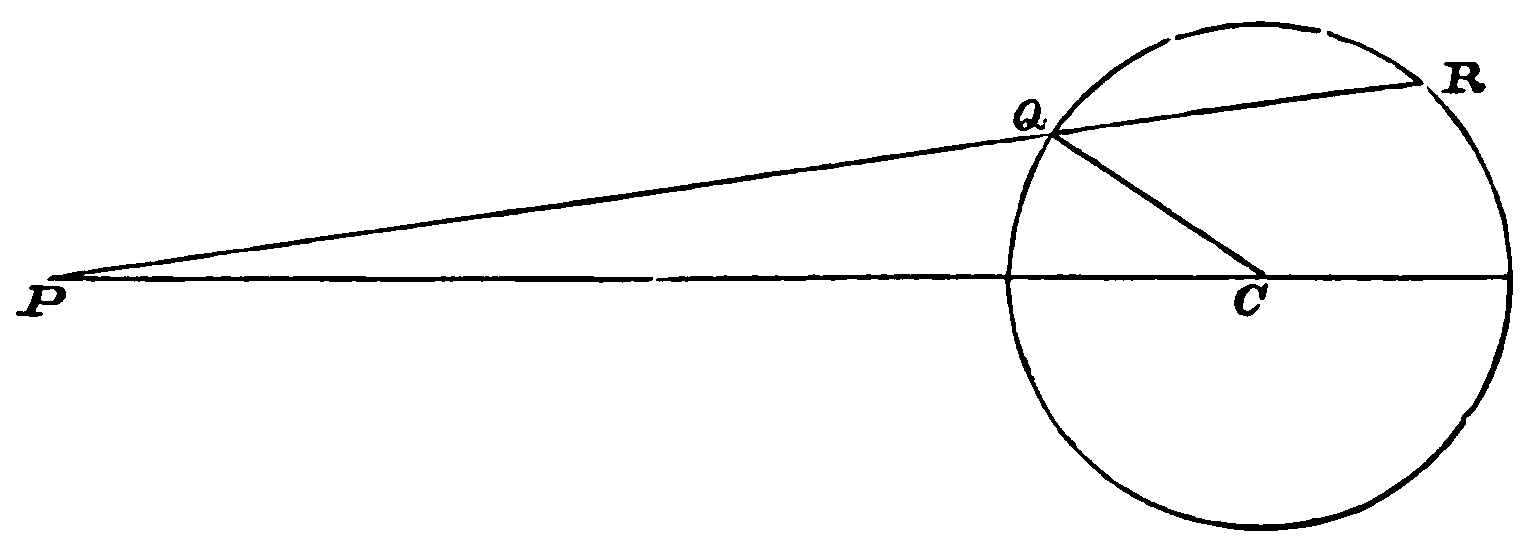
\includegraphics[width=0.77\textwidth]{421.png}
\centering
\end{figure}

Let \(C\) be the centre, \(P\) the external particle; let \(k\) denote the
radius, and \(p\) the distance \(CP\).

Draw from \(P\) any straight line \(PQR\) to cut the circle. Let
\(CPQ=\theta\), and \(CQR = \phi\); let \(PQ=r_1\), and \(PR=r_2\).

The attraction of the element of the circumference of the circle
at \(Q\) maybe denoted by \(\xp\dfrac{r_1d\theta\sec\phi}{{r_1}^2}\), and the attraction of the element
of the circumference at \(R\) by \(\xp\dfrac{r_2 d\theta\sec\phi}{{r_2}^2}\).

Hence the attraction of the two elements resolved along \(PC\)
\[=\frac{(r_1+r_2)\sec\phi\cos\theta\,d\theta}{r_1 r_2}=\frac{2p\cos^2\theta\sec\phi\,d\theta}{p^2-k^2}.\]

Now \(k \sin \phi = p \sin \theta\); therefore \(k \cos \phi d\phi = p \cos \theta d \theta\). Hence
the whole attraction of the circle
\[= \frac{4k}{p^2 - k^2}\int_{0}^{\tfrac{\pi}{2}}\cos\theta d\phi=\frac{4k}{p^2-k^2}\int_{0}^{\tfrac{\pi}{2}}\bigsurd\left(1-\frac{k^2}{p^2}\sin^2\phi\right)d\phi.\]

Thus the whole attraction is expressed as a complete elliptic
integral of the second order.
%%-----File: 422.png-----%%

Plana's result involves two complete elliptic integrals; one of
the first order and one of the second order; see his page 401 at
the top. He rather has in view a point within the circle, but the
requisite slight modification is easily made. His result can be
made to agree with that just given by means of the known properties
of complete elliptic integrals.

We may put the above expression thus
\[\frac{4k}{p\xsurd(p^2-k^2)}\int_{0}^{\tfrac{\pi}{2}}\bigsurd\left(\frac{p^2-k^2\sin^2\phi}{p^2-k^2}\right)d\phi.\]

As \(p\) diminishes, the factor outside the integral sign increases;
and so also does the expression under the integral sign. Thus the
attraction continually increases as \(P\) approaches the circumference;
this might probably have been anticipated, though the demonstration
is not immediately obvious.

\Section
1475. The second problem considered by Plana is the attraction
exerted by a circular lamina on a particle which is not necessarily
in the plane of the circle.

This occupies pages 408\dots 421. Here, as in the first problem,
the expressions obtained for the components of the attraction
involve elliptic integrals.

\Section
1476. On his page 410, Plana omits \(p\) in the second term of
his expression for an attraction. The error is obvious because it
makes the two terms of his expression of \textit{different dimensions}.
Nevertheless the error is continued on pages 417, 418, and 421.
There are several instances of this kind of error or misprint in
the memoir. It is strange that such an elementary consideration
as the necessity of having the various terms of an expression of the
same dimension should apparently have been quite disregarded in
writing the memoir, or in correcting the press.

\Section
1477. On his page 416, Plana says:
\begin{squote}
\dots\ il me semble qu'il conviendrait d'employer ici les formules données
par Cotes pour avoir des valeurs approchées des intégrales.
\end{squote}

I suppose that Plana here refers to pages 30\dots 33 of the Chapter
\textit{De Methodo Differentiali Newtoniana} by Cotes. They relate to
what we should now speak of as the approximate calculation of
the area of a curve by the method of equidistant ordinates.
%%-----File: 423.png-----%%

\Section
1478. On his page 417, Plana says:
\begin{squote}
Je présume, que à l'aide des formules précédentes on peut démontrer
qu'un point placé entre les centres de deux cercles qui ne se coupent
pas doit prendre un mouvement oscillatoire sur la ligne qui joint les
centres des cercles sans pouvoir jamais atteindre la circonférence du
plus petit cercle.
\end{squote}

It is not quite clear to me what Plana means. But I presume
that one circle is supposed to fall entirely \textit{within} the other; or
we may for facility of conception suppose the two circles parallel,
but indefinitely close, and the particle to move between them.

Of course he cannot mean the two circles to be in the same
plane, and one quite without the other. For in such a case
there is indeed a position of equilibrium for a particle on the line
joining the centres and between the two circumferences: but the
equilibrium is \textit{unstable}, and if the particle is moved towards either
circle, it will move up to contact with that circle. This follows
from the fact that if a particle in the plane of a circle, outside the
circle, move \textit{towards} the circle, the attraction \textit{continually increases.}
This fact is established by supposing the circle decomposed into
thin strips at right angles to the straight line on which the particle
is supposed to move; for the attraction of a strip varies
inversely as the distance from the particle, and directly as the
sine of half the angle subtended by the strip at the particle:
hence the attraction of every strip increases as the particle approaches
the circle.

\Section
1479. On his pages 418\dots 420 Plana gives some numerical
calculations as to the attraction of a thin ring, like that of Saturn,
on a particle near the inner or outer boundary. He uses his
results to throw doubts on some remarks made by Laplace
in his sixth memoir: see Art.\ 871.

\Section
1480. I will give here a simple investigation of a problem
connected with this section of Plana's memoir.

Find the attraction exerted by a circular cylinder on a particle
placed in contact with the curved surface at a point equally
distant from the ends of the cylinder.
%%-----File: 424.png-----%%

Let \(2h\) be the height of the cylinder, and \(a\) the diameter of
the cylinder.

Take the origin at the point considered; let the axis of \(x\) be
the normal at this point, and the axis of \(z\) the generating line of
the cylinder.

Then the resultant attraction is obviously directed along the
axis of \(x\), and is equal to
\[\iiint\frac{x\,dx\,dy\,dz}{(x^2+y^2+z^2)^{\frac{3}{2}}},\]
the integration extending over the whole cylinder. Integrate
with respect to \(z\); the limits are \(-h\) and \(h\): thus we obtain
\[2h\iint\frac{x\,dx\,dy}{(h^2+r^2)^{\frac{1}{2}}\,r^2},\]
where \(r^2\) stands for \(x^2+y^2\).

Transform in the usual way to polar coordinates; thus we
obtain
\[2h\iint\frac{\cos\theta\,d\theta\,dr}{(h^2+r^2)^{\frac{1}{2}}}.\]

Integrate with respect to \(r\); the limits are \(0\) and \(a\cos\theta\);
thus we obtain
\[2h\int\cos\theta\log\frac{\xsurd(h^2+a^2\cos^2\theta)+a\cos\theta}{h}d\theta.\]

The limits for \(\theta\) are \(-\xp\dfrac{\pi}{2}\) and \(\xp\dfrac{\pi}{2}\). Integrate by parts, and
the integral reduces to
\[4ah\int_{0}^{\tfrac{\pi}{2}}\frac{\sin^2\theta\,d\theta}{\xsurd(h^2+a^2\cos^2\theta)}.\]

We may express this as
\[\frac{4h\xsurd(h^2+a^2)}{a}(F-E),\]
where \(F\) and \(E\) denote complete elliptic integrals of the first
and second order respectively; the modulus being \(\xp\dfrac{a}{\xsurd(h^2+a^2)}\).
%%-----File: 425.png-----%%

This is exact. If we suppose \(h\) very small compared with \(a\),
we have approximately
\[F = \log\frac{4\xsurd(a^2+h^2)}{h},\,\text{ and }\,E = 1;\]
so that finally the attraction approximately
\[= 4h\left(\log\frac{4a}{h}-1\right).\]

It will be found that this agrees with a result given by Plana
on his page 418, after we correct the mistake noticed in Art.\ 1476.
We must in his formula suppose \(p = k\), and double the result to
get the attraction of the whole cylinder.

For a numerical example suppose \(h = \xp\dfrac{1}{30}\) and \(a = 2\); we get
\(\xp\dfrac{4}{30}\,(\log 240 - 1)\), that is \(\xp\dfrac{4}{30}\) of \(4·48064\), that is \(·59742\). This
agrees with the result given by Plana on his page 419 in the
form \(2\times·29871\).

For another example suppose \(h = \xp\dfrac{1}{30}\) and \(a = \xp\dfrac{14}{5}\); we get
\(\xp\dfrac{4}{30}(\log336-1)\), that is \(\xp\dfrac{4}{30}\) of \(4·81711\), that is \(·64228\). This
does not agree with the result given by Plana on his page 419
in the form \(2\times·342933\).

\Section
1481. The third problem considered by Plana is the attraction
of a right cylindrical surface with a circular base on a particle
in the plane of the base. This occupies pages 422\dots 445. As
before, the expressions obtained involve elliptic integrals.

\Section
1482. In the particular case in which the height of the
cylinder is infinite, the attraction on an internal particle resolved
along the plane of the base is zero. This may be easily verified.
For suppose the cylinder to extend to infinity both above and
below the plane in which the particle is situated; then the attraction
vanishes, as may be shewn by a process like that of Newton
for an ellipsoidal shell. Hence, as the attractions of the parts
above and below the plane resolved along the plane are obviously
equal, each must vanish. In exactly the same manner, if a
particle be placed inside an ellipsoidal shell, at any point of a
%%-----File: 426.png-----%%
principal plane, the attraction of each half into which the principal
plane divides the shell resolved along the plane is zero.

\Section
1483. There are numerous misprints in this section. For
instance, on page 427 in Plana's formulæ (\textit{e}) and (\textit{i}), for \(2\lambda - 1\)
read \(\lambda\). This misprint is obvious from the principle of dimensions
to which I have referred in Art.\ 1476; the misprint extends
its influence over many of the subsequent formulæ.

\Section
1484. On his pages 439\dots 443 Plana investigates the values
of the following definite integrals:
\[
\int_{-\alpha}^\alpha \tan^{-1}
\frac{\beta\xsurd (\alpha^2 - x^2)}{\alpha (q - x)} dx
\text{ and }
\int_{-\alpha}^\alpha x \tan^{-1}
\frac{\beta \xsurd (\alpha^2 - x^2)}{\alpha(q - x)} dx.
\]
His process may be much improved.

Assume with him \(x = \xp\dfrac{(y^2 - 1) \alpha}{y^2 + 1}\); then the definite integrals
become
\[
4\alpha \int_0^\infty \frac{y \,dy}{(1 + y^2)^2} \tan^{-1}
\frac{2\beta y}{q + \alpha + y^2 (q - \alpha)},
\]
and
\[
4\alpha^2 \int_0^\infty \frac{y (y^2 - 1) dy}{(1 + y^2)^3} \tan^{-1}
\frac{2\beta y}{q + \alpha + y^2(q - \alpha)}.
\]

After this his process becomes very laborious. A better way
will be to assume
\[
\tan^{-1} \frac {2\beta y}{q + \alpha + y^2 (q - \alpha)}
= \tan^{-1} My - \tan^{-1} Ny;
\]
this gives
\[
M - N = \frac{2\beta}{q + \alpha}, \quad MN = \frac{q - \alpha}{q + \alpha};
\]
thus
\[
M + N = \frac{2}{q + \alpha} \xsurd\{\beta^2 + q^2 - \alpha^2\}.
\]

Hence \(M\) and \(N\) are known.

Consider the first integral, which Plana denotes by \(X\), so that
\[
X = 4\alpha \int_0^\infty (\tan^{-1} My - \tan^{-1} Ny) \frac{y dy}{(1 + y^2)^2}.
\]

Integrate by parts; thus
\[
X = 2\alpha \int_0^\infty
\left(\frac{M}{1 + M^2 y^2} - \frac{N}{1 + N^2 y^2}\right)
\frac{dy}{1 + y^2} \tag{1}.
\]
%%-----File: 427.png-----%%
But
\begin{gather*}
\int_0^\infty \frac{dy}{(1 + h^2y^2)(1 + k^2y^2)} = \frac{1}{h^2 - k^2}
\int_0^\infty \left(\frac{h^2}{1 + h^2y^2} - \frac{k^2}{1 + k^2y^2}\right) dy \\
= \frac{1}{h^2 - k^2} (h - k) \frac{\pi}{2} = \frac{\pi}{2(h + k)} \tag{2}.
\end{gather*}

From (1) and (2) we see that
\begin{align*}
X &= \pi\alpha \left(\frac{M}{M + 1} - \frac{N}{N + 1}\right)
= \frac{(M - N)\pi\alpha}{1 + M + N + MN}\\
&= \frac{\alpha\beta\pi}{q + \xsurd (q^2 + \beta^2 - \alpha^2)}
= \frac{\pi\alpha\beta \{q - \xsurd (q^2 + \beta^2 - \alpha^2)\}}{\alpha^2 - \beta^2}.
\end{align*}

Now consider the second integral, which Plana denotes by \(X'\).
Integrate by parts; thus
\[
X' = 2\alpha^2 \int_0^\infty
\left(\frac{M}{1 + M^2y^2} - \frac{N}{1 + N^2y^2} \right)
\frac{y^2dy}{(1 + y^2)^2} \tag{3}.
\]

If we differentiate (2) with respect to \(k\) we find that
\[
\int_0^\infty \frac{y^2dy}{(1 + h^2y^2)(1 + k^2y^2)^2}
= \frac{\pi}{4k(h + k)^2} \tag{4}.
\]

From (3) and (4) we see that
\[\begin{aligned}
X' &= \frac{\pi\alpha^2}{2}
\left\{\frac{M}{(M + 1)^2} - \frac{N}{(N + 1)^2}\right\}\\
&= \frac{\pi\alpha^2}{2} \frac{M(N + 1)^2 - N(M + 1)^2}{(M + 1)^2(N + 1)^2}\\
&= \frac{\pi\alpha^2}{2} \frac{(M - N)(1 - MN)}{(M + 1)^2(N + 1)^2}\\
&= \frac{\pi\alpha^3}{2}
\frac{\beta}{\{q + \xsurd(q^2 + \beta^2 - \alpha^2)\}^2}\\
&= \frac{\pi\alpha^3\beta}{2}
\left\{\frac{q - \xsurd(q^2 + \beta^2 - \alpha^2)}{\alpha^2 - \beta^2}\right\}^2.
\end{aligned}\]

Thus, as Plana says on his page 443, we have
\[
X' = \frac{\alpha}{2\pi\beta} X^2;
\]
he adds: ``ce qui constitue un théorème assez remarquable.''
%%-----File: 428.png-----%%

Let there be an infinite right elliptic cylinder; let \(2\alpha\) be the
major axis and \(2\beta\) the minor axis of the ellipse. Then \(4X\) expresses
the attraction of the cylinder on a particle situated on the
axis major produced, and at a distance \(q\) from the centre. This is
easily shewn by cutting up the cylinder into infinitesimal rods
parallel to the generating lines, and summing the attractions of
the rods which form a slice at right angles to the major axis of the
ellipse.

\Section
1485. The last problem considered by Plana is the attraction
of an infinite right elliptic cylinder on an external particle. This
occupies pages 445\dots 450.

Let \(f\) and \(g\) be the coordinates of the attracted particle, estimated
from a fixed point in a plane at right angles to the generating
lines of the cylinder. Let \(V\) denote the potential of the
cylinder. Then we know that \(V\) will be a function of \(f\) and \(g\)
determined by
\[\frac{d^2V}{df^2}+\frac{d^2V}{dg^2} = 0.\]
Hence
\[V = \phi\{f + g\xsurd(-1)\} + \psi\{f - g\xsurd(-1)\},\]
where \(\phi\) and \(\psi\) denote functions at present undetermined.

The resolved attractions we know are equal to \(\xp\dfrac{dV}{df}\) and \(\xp\dfrac{dV}{dg}\)
respectively. Hence we obtain for these resolved attractions expressions
like that given for \(V\).

Now Plana obtains these expressions for the resolved attractions
without any use of the potential; and this is the only
novelty in his solution: see his page 449.

\Section
1486. In the fifth volume of De Zach's \textit{Correspondance Astronomique \dots},
published in 1821, is a note by Plana entitled, \textit{Note sur
la densité et la pression des couches du sphéroïde terrestre}; it occupies
pages 68\dots 79 of the volume.

\Section
1487. The note relates to the law of density and the law of
pressure discussed by Laplace in the \textit{Connaissance des Tems} for
1822: see Arts.\ 1285 and 1325.

Plana calculates the values of the density and of the pressure
at various depths below the surface of the Earth by Laplace's
%%-----File: 429.png-----%%
formulæ; but he adds nothing to the theoretical investigations.
He also makes some comparison of the theory with observations.

I will notice two or three points which present themselves.

\Section
1488. His formula (2) on page 70 involves some strange mistake
or misprint; the term \(\xp\left(\dfrac{5\pi}{6\xsurd6}+\dfrac{1}{3\xsurd2}\right)^2\) is wrong.

\Section
1489. Plana works out in detail the comparison of theory
with observation, to which Laplace himself gave some attention:
see Art.\ 1329. By this comparison Plana arrives at the result that
the ratio of the Moon's mass to the Earth's mass is \(·0122651\), which
he says lies between \(\xp\dfrac{1}{82}\) and \(\xp\dfrac{1}{83}\); but it should be between \(\xp\dfrac{1}{82}\)
and \(\xp\dfrac{1}{81}\).

Plana says:
\begin{squote}
La masse de la lune \(·0122651\) diffère sensiblement de la fraction
\(\xp\dfrac{1}{68·5}\) que l'on obtient autrement comme l'on sait. Mais malgré cela on
doit, ce me semble, admettre, que cette loi de la densité des couches du
sphéroïde terrestre s'accorde assez bien avec l'ensemble des phénomènes
connus. Cela posé, il me paraît certain, que la valeur de
\[\frac{\displaystyle\int \rho a^4\,da}{\displaystyle\int \rho a^2\,da} = ·27216,\]
trouvée par M. le Baron de \textit{Lindenau} (voyez Éphémérides de Berlin
pour 1820, page 211) doit etre trop éloignée de la véritable, puisque la
théorie précédente donne \(·485967\) avec un degré d'approximation plus
plausible.

Au reste, il est essentiel d'observer, que le rapport de ces deux intégrales
définies a été calculé par M. de \textit{Lindenau} à l'aide de la formule
\[\frac{\displaystyle\int \rho a^4\,da}{\displaystyle\int \rho a^2\,da} = \frac{3}{5}\left(1 -\frac{j}{2\epsilon}\right),\]
qui lui a été communiquée par M. \textit{Gauss}.

J'ignore dans ce moment le juste degré d'approximation de cette formule
ainsi que le moyen de la dériver de la condition de l'équilibre de
l'océan\dots.
\end{squote}
%%-----File: 430.png-----%%

I have expressed the formula given by Gauss in my own notation;
\(\epsilon\) is the Earth's ellipticity and \(j\) is, as usual, the ratio of the
centrifugal force at the equator to the attraction there.

I am, like Plana, quite ignorant as to the origin of the formula.
I have no faith in it. It looks to me as if Gauss had intended to
suppose the Earth to be composed of similar elliptic strata, surrounded
by a film of fluid; then the \(\xp\dfrac{3}{5}\) must be cancelled. See
equation (2) of Art.\ 323; and there suppose \(\epsilon\) constant.

\Section
1490. Plana brings evidence from a comparison of the lunar
theory with observation to confirm the value of the moon's mass
he had obtained, which, as we have seen, was rather smaller than
the value found otherwise. The present received value seems
still smaller than that adopted by Plana.

\Section
1491. Plana concludes thus:
\begin{squote}
Telles sont toutes les principales conséquences qui dérivent immédiatement
de la loi supposée pour la densité des couches du sphéroïde terrestre.
En considérant l'ensemble des phénomènes, l'accord est tellement
satisfaisant, que l'on paraît autorisé à regarder cette loi comme celle de
la nature.
\end{squote}

Perhaps this is expressed rather too strongly. Let us consider
what is meant by \textit{l'ensemble des phénomènes}.

Taking with Legendre and Laplace, as in Art.\ 1326, for the
density the expression \(A\xp\dfrac{\sin an}{a}\), it is found that if \(n\) is supposed
equal to \(\xp\dfrac{5\pi}{6}\), the ellipticity of the Earth agrees well with observation.
But we can hardly say that this gives any evidence in favour
of the supposed law of density; the coincidence has in fact been
secured by a proper selection of a certain arbitrary constant.
Thus all that seems to remain is that the value of \(\xp\dfrac{\xp\displaystyle\int \rho a^4\,da}{\xp\displaystyle\int \rho a^2\,da}\), as
found by our expression for \(\rho\), agrees reasonably well with the phenomena
of precession and nutation.
%%-----File: 431.png-----%%

\Section
1492. The next memoir by Plana which we have to consider
is entitled \textit{Mémoire sur différens procédés d'intégration, par lesquels
on obtient l'attraction d'un ellipsoïde homogène dont les trois
axes sont inégaux, sur un point extérieur}. This memoir occupies
pages 189\dots 270 of Crelle's \textit{Journal für \dots\ Mathematik}, Vol.\ \textsc{xx}.,
which was published in 1840.

\Section
1493. Plana begins by alluding to some discussions in the
Academy of Paris, which we have seen took place towards the
close of Poisson's career: see Art.\ 1404. He says that he drew
up the memoir principally for his own instruction, after reading
that by Poisson in Vol.\ \textsc{xiii}.\ of the Memoirs of the Academy of
Paris. On reflection his memoir seemed to him to gain a greater
degree of importance by the novelty of the methods employed,
either to obtain the known results or to illustrate them.

\Section
1494. The memoir is divided into four sections; each section
might be considered in certain respects as an independent memoir:
but in uniting them they afforded mutual assistance.

\Section
1495. The following sentences from the introduction may
be noticed as giving Plana's opinion on a point discussed between
Poisson and Poinsot:
\begin{squote}
On verra dans le quatrième paragraphe quelle est mon opinion et ma
manière de considérer la solution donnée par \textit{Legendre} en 1788. C'est
un chef-d'-œuvre d'analyse; si par le mot \textit{analyse}, on veut bien entendre
une suite de transformations des formules primitives dans lesquelles le
raisonnement est en partie remplacé par le mécanisme du calcul. Abstraction
faite de la longueur des calculs c'est, à mon avis, la solution la
plus directe qu'on ait donné de ce problème jusqu'à ce jour.
\end{squote}

Plana proceeds then to explain in what sense he takes the
word \textit{direct}, so as to justify the high commendation he thus pronounces
on Legendre's solution: but the remarks do not altogether
commend themselves to my judgement.

\Section
1496. The memoir is useful as bringing together various
investigations which were originally published in other places,
and supplying some explanatory comment, yet it cannot be said
to contain anything essentially new and important.
%%-----File: 432.png-----%%

\Section
1497. Suppose we have a given ellipsoid, and we wish to
determine a confocal ellipsoid which shall pass through a given
point: this problem we know occurs in Ivory's mode of treating
the attraction of an ellipsoid. The problem leads to a cubic
equation. Plana's first section is devoted to the discussion of
this problem: it occupies his pages 193\dots 206.

\Section
1498. The following passage may be noticed:
\begin{squote}
\dots\ \textit{Legendre} avait dit (et Mr.\ \textit{De Pontécoulant} a répété d'après lui,
voyez p.\ 354 du second volume de sa Théorie analytique du systême du
monde) que cette équation n'a qu'une seule racine réelle (voyez p.\ 542
du tome 1\textsuperscript{er} de son Traité des fonctions elliptiques); mais la réalité de
ses trois racines est maintenant hors de doute.
\end{squote}

Plana is wrong in his charge so far as relates to Pontécoulant.
The equation which Pontécoulant takes is
\[\frac{a^2}{k^2}+\frac{b^2}{k^2 + e^2}+\frac{c^2}{k^2 + e'^2} = 1;\]
this equation has doubtless three roots for \(k^2\), namely, one positive
and two negative, but the latter do not make \(k^2\) real: so there is
but one \textit{real} value of \(k^2\).

Legendre indeed is incautious; his equation is
\[\frac{f^2}{\alpha^2 + \xi}+\frac{g^2}{\beta^2 + \xi}+\frac{h^2}{\gamma^2 + \xi} = 1;\]
and he says that there is only one real value of \(\xi\): but the
context suggests that he means only one real \textit{positive} value.

\Section
1499. Plana's second section relates to the equation of the
cone which has its vertex at a given point and circumscribes a
given ellipsoid; it occupies pages 206\dots 216. He shews how to
put this equation in its simplest form by changing the axes of coordinates.
The last twelve lines of the section contain some
troublesome misprints in formulæ which relate to the circular
sections of the cone.

\Section
1500. Plana's third section purports to treat of the formulæ
for determining the attraction of an indefinitely thin ellipsoidal
shell bounded by similar surfaces, on an external particle; it occupies
%%-----File: 433.png-----%%
pages 216\dots 240. But the title is inadequate, as there are
many other formulæ in the section besides those which relate to
the attraction of the film bounded by homothetical ellipsoids.

\Section
1501. In the beginning of this section Plana draws various
useful deductions from the known formulæ for the attraction of an
ellipsoid on an external point. We will reproduce some of these;
but it will be sufficient for us to confine ourselves to one of the
three components of the attraction.

Denote by \(X\) the component considered in Art.\ 885. Then
with the notation there employed we have
\[X =\frac{ 4\pi abcf}{k}\int_{0}^{1}\frac{x^2\, dx}{\sqrt{k^2 + (b^2 - a^2)x^2}\sqrt{k^2 + (c^2 - a^2) x^2}},\]
where \(k^2\) has to be found from an equation there given.

Put \(m = \xp\dfrac{a^2}{b^2},\quad n =\xp\dfrac{ a^2}{c^2},\quad k^2 = a^2 (1 + \nu)\).

Then the equation for determining \(\nu\) and \(k^2\) becomes
\[\frac{f^2}{1+\nu}+\frac{mg^2}{1+m\nu}+\frac{nh^2}{1+n\nu}= a^2\tag{1},\]
and we have
\[X=\frac{4\pi f}{\xsurd(1+\nu)}\int_{0}^{1}\frac{x^2\, dx}{\sqrt{m(1+\nu)+(1-m)x^2}\sqrt{n(1+\nu)+(1-n)x^2}}.\]

Now if we form \(\xp\dfrac{dX}{d\nu}d\nu\), we shall obtain the expression for the
component attraction of a film bounded by homothetical ellipsoids;
because by the change of \(a\) into \(a + da\) and of \(\nu\) into \(\nu + d\nu\), we
pass from one ellipsoid to a similar, similarly situated, and concentric
ellipsoid infinitesimally different from the former.

In this way we can verify Poisson's theorem as to the attraction
of a certain film: see Art.\ 1394. Poisson himself says that he
did this: his words are quoted in Art.\ 1405. If however we
differentiate with respect to \(\nu\) the value of \(X\) in the form in which
we have left it, the integral sign does not obviously disappear. It
is convenient to change the variable. Put
\[x^2 =\frac{ 1 + \nu}{1 + u};\]
%%-----File: 434.png-----%%
then we obtain
\[X = 2\pi f\int_{\nu}^{\infty}\frac{ (1 + u)^{-\frac{3}{2}}\, du}{\sqrt{(1 + mu)(1 + nu)}}\tag{2}.\]

Therefore
\[\frac{dX}{d\nu} =-\frac{2\pi f(1 + \nu)^{-\frac{3}{2}}}{\sqrt{(1 + m\nu)(1 + n\nu)}}.\]

Hence the component \(\xp\dfrac{dX}{d\nu} d\nu\) is expressed free from the integral
sign.

Similarly the other components can be expressed free from the
integral sign.

Plana's formulæ give the direction of the resultant attraction;
but we do not delay on this point.

\Section
1502. Put
\[(1 + u) a^2 = {v_1}^2,\quad (1 + mu) b^2 = {v_2}^2,\quad (1 + nu)c^2 = {v_3}^2.\]

Then (1) becomes
\[X = 4\pi fabc \int_{k}^{\infty}\frac{ dv_{1}}{{v_1}^2 v_2 v_3}\tag{3}.\]

This form agrees with that given by Rodrigues; see Art.\ 1396.

Thus, as Plana observes, Rodrigues had only one step to take
in order to obtain from his formulæ the attraction of the film.
He had in fact only to pass from (3) to (2), and then differentiate
with respect to \(\nu\). However Rodrigues did not take this step;
and the result was first given by Poisson.

\Section
1503. Plana finishes the section with remarks which demand
some criticism.

By a certain transformation of the expression already given
for \(X\) he obtains a result of the form
\[X = 4\pi \int f(\omega)\,d\omega,\]
where the limits of the variable \(\omega\) are \(0\) and \(\xsurd A'\).

Then he says he will interpret this geometrically. Now a
certain series of cones has presented itself in his investigations,
determined by a parameter which varies between \(0\) and \(\xsurd A'\).
%%-----File: 435.png-----%%
Hence he infers that the resolved attraction of that part of the
ellipsoid which is contained between the cones corresponding to
the values \(\omega\) and \(\omega + d\omega\) is \(4\pi f(\omega)\,d\omega\). This is quite unsound.
We might on the same ground take the expression for \(X\) given in
the beginning of Art.\ 1501, change \(x\) into \(\xp\dfrac{\omega}{\xsurd A'}\) so that \(X\) becomes
say \(\xp\displaystyle\int\psi(\omega)\, d\omega\), and then assert that \(\psi(\omega)\, d\omega\) represents the attraction
of the conical element. In other words Plana proves fairly that
\(4\pi\xxp\displaystyle\int f(\omega)\, d\omega\) between the specified limits represents the resolved
attraction of the ellipsoid; but he has \textit{no ground whatever} for his
assertion as to the geometrical meaning of \(4\pi f(\omega)\, d\omega\). The assertion
is indeed true, for Legendre demonstrated it; but Plana gives
no demonstration of his assertion.

\Section
1504. The fourth section of Plana's memoir is devoted to the
demonstration of a certain formula of Legendre's; this section
occupies pages 240\dots 270. The formula is that to which we
alluded in the preceding Article.

In our account of Legendre's third memoir we have stated that
Legendre supposes a certain series of cones having their common
vertex at the attracted point. Two consecutive conical surfaces
will determine a conical shell; Legendre finds an expression for
the attraction at the vertex of that part of such a shell which is
bounded by the attracting ellipsoid. This expression is that of his
formula \((g')\) in page 479: it is
\[\frac{2\pi\omega^2 d\omega}{F}\left\{\frac{G}{\xsurd H}+\frac{G'}{\xsurd H'}\right\},\]
where \(\omega\) is a parameter which determines the conical shell, and
the capital letters denote certain complicated functions of the
parameter, the coordinates of the attracted point, and the semiaxes
of the ellipsoid.

Legendre devotes his pages 470\dots 479 to the investigation of
the formula. As I have said however his process is rather indicated
than worked out.
%%-----File: 436.png-----%%

\Section
1505. Now Plana gives the operations in detail; and this
constitutes the business of his thirty pages. He says himself on
his page 240:
\begin{squote}
Les artifices de calcul par lesquels \textit{Legendre} est parvenu à une
démonstration directe de la formule \dots\ sont fort ingénieux. Mais, il est
impossible d'apprécier au juste le degré de la complication et le mérite
de la difficulté vaincue, sans suivre pas à pas les transformations et les
réductions à travers lesquelles on doit passer pour mettre en évidence
la propriété caractéristique du résultat obtenu par le procède de son
intégration. Malgré les indications laissées par \textit{Legendre} il n'est pas
fort aisé (du moine pour moi) de retrouver, ni les résultats intermédiaires
ni le résultat final. Je pense qu'il ne sera pas tout-à-fait inutile
d'exposer ici avec détail la marche que j'ai suivie par y parvenir.
\end{squote}

\Section
1506. I had myself gone over Legendre's work in his own
order and with his own notation, before I had seen Plana's
memoir. I find that the additional developments thus required
will fill about seven quarto pages like Plana's. To a patient
student such a course would not be more laborious than the study
of Plana's pages.

\Section
1507. Legendre effects a certain transformation which at first
sight does not appear to have produced any simplification. Plana
observes that perhaps it was only after trial justified by the subsequent
investigations that he found the advantage of his transformation.
Plana adds on his page 248:
\begin{squote}
Un récit naïf des tâtonnements de ce genre serait fort instructif;
mais, par des motifs difficiles à deviner, il est rare de rencontrer dans
les écrits des grands géomètres des exemples comparables à ceux qui
nous frappent en lisant les ouvrages d'\textit{Euler}.
\end{squote}

\Section
1508. Legendre's formula \((g')\) presents a very complicated
appearance; Legendre simplifies it by a peculiar process, not by
direct calculation: see what has been said with respect to this
point in Arts.\ 888 and 889. Plana appears to allude to this in
the last paragraph of his memoir; he says:
\begin{squote}
Le calcul dont nous venons de parler (fort pénible même dans le cas
particulier où le point attiré serait placé dans le plan d'une des trois
sections principales de l'éllipsoïde) est sans doute celui que Mr.\ Poisson
%%-----File: 437.png-----%%
qualifie \textit{d'inextricable}: mais la démonstration de \textit{Legendre} ne réclame
point, ni l'exécution effective de ce calcul, ni l'appui d'aucun théorême
dérivé d'une autre source. Le théorême qu'il avait en vue, et son expression
analytique sous la forme la plus simple, découlent des principes
les plus rigides du Calcul Intégral. L'état progressif de l'analyse
fait espérer que cette espèce de lacune laissée par \textit{Legendre} sera un jour
heureusement remplie. Il est même probable qu'elle le sera par un de
ces traits de génie qui attestent la force des principes, et la difficulté de
saisir le véritable mode d'en faire l'application.
\end{squote}

I do not feel quite certain as to Plana's meaning; but I presume
by \textit{le calcul} he means a simplification of Legendre's formula
\((g')\) by actual algebraical work. When he says that Legendre's
demonstration does not require this work, I suppose he means
that the peculiar process adopted by Legendre is sound; in this I
agree with him. Thus Plana, according to my view, is correct in
the sense he assigns to Poisson's word \textit{inextricable}; the meaning
being that at a certain stage Legendre could not obtain his desired
result by actual algebraical work, but adopted a peculiar
process. This actual algebraical work Plana describes on his
last page as ``effrayant pour le plus intrépide algèbriste.''

\Section
1509. The next memoir by Plana is entitled \textit{Note sur l'intégrale
\(\displaystyle\int\xp\dfrac{dM}{r}=V\), qui exprime la somme des élémens de la masse d'un
ellipsoïde, divisés respectivement par leur distance à un point attiré.}
This occurs in the same volume as the preceding memoir: it occupies
pages 271\dots 282.

\Section
1510. The memoir investigates a certain expression for the
potential of an ellipsoid which agrees with that given in Art.\ 1184.
Let the notation be as in Art.\ 1501; then the potential \(V\) is determined
by
\[V = -\pi \int_{\nu}^{\infty}\left\{\frac{f^2}{1+u}+\frac{mg^2}{1+mu}+\frac{nh^2}{1+nu}-a^2\right\}\frac{du}{\xsurd U}\tag{4},\]
where \(U = (1 + u) (1 + mu) (1 + nu)\).

For an external point \(\nu\) must be found by the equation (1) of
Art.\ 1501. For an internal point we must put zero for \(\nu\).
%%-----File: 438.png-----%%

Plana considered the potential for an internal point again
in a subsequent memoir. See the \textit{Astronomische Nachrichten},
Vol.\ \textsc{xxxvi}.\ page 172, and Art.\ 1543.

To justify his formula we observe that if we differentiate with
respect to \(f\), \(g\), or \(h\), we obtain a correct result. Thus, for example,
it gives
\[\frac{dV}{df} = -2\pi f \int_{\nu}^{\infty}\frac{ du}{(1 + u)\xsurd U},\]
for no term arises from the variation of \(\nu\), since the expression
under the integral sign vanishes when \(U=\nu\), by equation (1) of
Art.\ 1501.

Now this value of \(\xp\dfrac{dV}{df}\) is correct, because \(-\xp\dfrac{dV}{df}\) we know is equal
to the \(X\) of Art.\ 1501; and so we see that our result is true by
(1) of that Article.

In like manner, if we differentiate (4) with respect to \(g\) or to
\(h\), we obtain a correct result. Hence (4) must be true, provided
it is true for any special values of \(f\), \(g\), \(h\); that is, we have only
to shew that no arbitrary constant is required in (4).

Plana effects this comparison by calculating directly the value
of \(V\) for an external particle, and shewing that the expression
agrees with (4).

A simple mode is by shewing that when \(f\), \(g\), and \(h\) are infinite,
the expression for \(V\) in (4) vanishes as it should.

When \(f\), \(g\), \(h\) are infinite, we have \(\nu\) infinite by (1) of Art.\ 1501.

But \(\xp\dfrac{f^2}{1 + u}+\xp\dfrac{mg^2}{1 + mu}+\xp\dfrac{nh^2}{1 + nu}\) is numerically less than when
\(u=\nu\); so that it is finite. And \(\xsurd U\) is greater than \(u^{\frac{3}{2}}\xsurd (mn)\);
hence \(\displaystyle\int_{\nu}^{\infty}\xp\dfrac{\mathop{du}}{\xsurd U}\) vanishes when \(\nu\) is infinite; and so also does
\(\displaystyle\int_{\nu}^{\infty}\xp\dfrac{v\mathop{du}}{\xsurd U}\) if \(v\) be any finite quantity.

\Section
1511. Plana shews that his value of \(V\) involves a demonstration
of a result originally obtained by Jacobi and investigated
by Poisson: see Art.\ 1401.
%%-----File: 439.png-----%%

\Section
1512. If the value of \(V\) is required in a series proceeding
according to inverse powers of the distance of the attracted point
from the centre of the ellipsoid, Plana considers that the best
way would be to combine the methods of Laplace and Lagrange.
Laplace's method is that which is contained in the \textit{Mécanique
Céleste}, Livre \textsc{iii}.\ Chapitre \textsc{ii}. Lagrange's method is that to
which we allude in Art 1467. Plana applies both methods.

\Section
1513. The next memoir by Plana is entitled \textit{Appendice au
Mémoire sur l'attraction de l'ellipsoïde homogène imprimé dans le
Tome \textsc{xx}.\ de ce journal.} This memoir occupies pages 132\dots 146
of Crelle's \textit{Journal für \dots\ Mathematik}, Vol.\ \textsc{xxvi}., which was published
in 1843.

\Section
1514. In this memoir Plana gives in detail the operations
required in the third Section of Legendre's memoir: see Art.\ 880.

Legendre himself left much of the work to be done by the
reader. A patient student would find it perhaps as easy to fill up
the steps for himself in Legendre's memoir as to read Plana's.

Plana concludes thus:
\begin{squote}
On doit comprendre maintenant que l'analyse de \textit{Legendre} avoit
besoin de ce long développement, pour pouvoir saisir plusieurs des
motifs secrets qui ont guidée la marche de son calcul. J'ignore s'il est
permis de soutenir, que de tels motifs peuvent être aisément devinés
d'après le texte de \textit{Legendre}.
\end{squote}

\Section
1515. Two notes by Plana were published in the Turin
\textit{Memorie}, Vol.\ \textsc{xi}.\ 1851. The first note purports to relate to
Newton's Proposition \textsc{lxxi}., and the second note to Newton's
Propositions \textsc{lxxx}.\ and \textsc{lxxxiv}. The notes occupy pages 391\dots 406
of the volume.

\Section
1516. The notes may be said to consist of translations of
Newton's investigations respecting attractions into analytical
language. Thus, take Newton's Proposition \textsc{lxxi}. We have
seen in Art.\ 4, that Newton's investigation leads to this result:
the attraction \(= \xxp\dfrac{4\pi k\rho a}{c^2}\displaystyle\int \dfrac{p \mathop{dp}}{\xsurd(a^2 - p^2)}\), the integration being taken
%%-----File: 440.png-----%%
between proper limits. Thus we have \(\xxp\dfrac{4\pi k\rho a}{c^2}\displaystyle\int d\ldot\xsurd(a^2 - p^2)\) between
proper limits. Now \(\xsurd(a^2 - p^2)\) is equal to half a certain
chord in Newton's figure, which he calls \(HK\). Plana arrives at
this expression by a method somewhat different from that which
we have used.

\Section
1517. Plana gives what he considers an exposition of Newton's
mode of establishing his Proposition \textsc{lxx}; we may however state
briefly that the exposition is inaccurate. Plana asserts that
Newton uses the property about the intersecting chords of a circle;
Euclid \textsc{iii}.\ 35 is meant. Newton does not use this property:
he seems to use the equality of angles in the same segment.

\Section
1518. There is nothing important or remarkable in Plana's
analytical translations of Newton's processes; they are substantially
the same as would occur to any person acquainted with the
elements of the Differential and Integral Calculus, and had in
fact been given by Maupertuis in his memoir of 1732.

\Section
1519. Plana seems to think that Newton adopted geometrical
forms in order to conceal his peculiar methods. Thus he says:
\begin{squote}
Mais, Newton, qui, probablement, ne voulait pas dévoiler à ses
lecteurs toutes les ressources de ce calcul, alors naissant, a imaginé une
démonstration, où, le procédé de l'intégration est déguisé\dots.
\end{squote}

Again:
\begin{squote}
On ne peut éviter cette traduction algébrique sans nuire à la clarté,
et sans renforcer l'opinion que Newton ne voulait pas exposer ses découvertes
avec cette ingénuité qui les aurait rendues accessibles aux
hommes doués d'une médiocre intelligence.
\end{squote}

\Section
1520. The next memoir by Plana is contained in the \textit{Astronomische
Nachrichten}, No.\ 828, which was published in September
1852: this number forms part of Vol.\ \textsc{xxxv}.\ of the Journal.

The memoir consists of three parts, namely a \textit{Note} and two
\textit{Additions}. The memoir is entitled \textit{Note sur la densité moyenne de
l'écorce superficielle de la Terre.}

\Section
1521. Plana begins thus:
\begin{squote}
C'est un fait incontestable, que la densité des couches elliptiques du
sphéroïde terrestre est croissante depuis la surface jusqu'au centre. La
%%-----File: 441.png-----%%
loi de cet accroissement est inconnue; mais comme elle est intimement
liée à tous les phénomènes qui dépendent du mouvement de rotation de
la Terre autour de son centre de gravité, on peut faire des hypothèses
sur son expression algébrique, et comparer ensuite les résultats qu'elles
fournissent à ceux que l'observation a fait connaître avec un précision
suffisante. Je vais examiner, sous ce point de vue, la plus simple de
toutes les hypothèses, proposée par \textit{Laplace} à la page 46 du cinquième
volume de la \textit{Mécanique Céleste}.
\end{squote}

\Section
1522. Thus Plana's Note relates to the hypothesis proposed
by Laplace in the page just cited. The hypothesis is that the
density increases from the surface to the centre in Arithmetical
Progression. The hypothesis is expressed symbolically in the
following manner. Let \((\rho)\) denote the density at the surface, \(\rho\)
the density at the distance \(a\) from the centre, the mean radius of
the Earth being taken as unity. Then \(\rho = (\rho) \{1 + e - ea\}\), where
\(e\) is some constant to be determined.

Taking the density of the sea for unity, Laplace assumed that
\((\rho) = 3\), which is about the density of granite: then he obtained
\(e = 2·349\).

\Section
1523. Plana considers that \(3\) is too large a value for \((\rho)\). He
does not assume a value for \((\rho)\), but considers that it has been
well established by the experiments of Reich that the \textit{mean}
density of the Earth is \(5·44\). Taking this for granted, and employing
certain formulæ from other parts of the \textit{Mécanique Céleste},
Plana finds that \(e\) is about \(7·8907\).

\Section
1524. The Note contains nothing new in theory; it consists
entirely of numerical calculation. I have not verified this. Indeed
there are some difficulties, which though not very serious
discourage any attempt to go over the work. I will state them,
as some other student may be fortunate enough to explain them.

(1) I do not see how the coefficient of \(\mu\) in Plana's equation
(6) is obtained; apparently it should be the product of \(·12065\)
and \(·0163\); but it is not equal to this.

(2) In comparing his equations (6) and (7) the sign of the
coefficient of \(\mu\) seems arbitrarily changed from \(-\) to \(+\).

(3) Having arrived at his equation (17) Plana seems to assert
that the density at the centre is more likely to be greater than
%%-----File: 442.png-----%%
\(16·301\) than less. I cannot conjecture how he obtained any
knowledge as to the numerical value of the density at the centre.

(4) Towards the beginning of his Note, Plana says that
\(16·27\) is the density at the centre; but from his equation (17) it
would appear that this density is greater than \(16·301\). I cannot
reconcile these statements.

(5) Plana says that Legendre's law of density leads to less
satisfactory results. According to this law, see Art.\ 1326,
\[\rho =\frac{(\rho) \sin an}{a \sin n}.\]

If \(n =\xp\dfrac{5\pi}{6}\), Plana obtains for the density at the centre \(9·4235\);
and if \(n =\xp\dfrac{7\pi}{8}\), he obtains \(12·89\). Then I gather that these results
are unsatisfactory to him, because they do not make the
density at the centre great enough. But, as I have already said, I
cannot conjecture how Plana obtained any knowledge as to what
the density at the centre ought to be.

(6) Suppose that in the last expression for \(\rho\) we give to \(n\)
a small increment \(\delta n\); then Plana says that \(\rho\) becomes
\[\frac{(\rho) \sin an}{a \sin n} +\frac{(\rho)\delta n \sin (n - an)}{\sin^2n}.\]

It seems to me that the second term should be
\[(\rho)\delta n\frac{a \cos an \sin n - \sin an \cos n}{a \sin^2 n}.\]

\Section
1525. Laplace obtained for the mean density of the Earth
\(4·76\). Plana finds that the same value of the mean density would
follow from supposing \((\rho) = 1·6\), instead of \((\rho) = 3\); and remarks
that this is rather singular.

\Section
1526. It appears from the conclusion of the Note that Plana
undertook the discussion at the request of Humboldt. Towards
the beginning of the Note Plana refers to what Humboldt had
said on the subject in his \textit{Kosmos}, Vol.\ \textsc{i}.\ page 177, of the
German edition. See Vol.\ \textsc{i}.\ page 159, of Sabine's English translation,
fifth edition.

\Section
1527. In the first Addition to his Note, Plana adverts to the
determination of the density of a mountain by the aid of pendulum
%%-----File: 443.png-----%%
experiments. Laplace had touched on this subject in the
\textit{Mécanique Céleste}, Vol.\ \textsc{v}.\ pages 55 and 56. Plana adds nothing
of importance.

Plana gives in this Addition the calculation necessary to solve
the following problem. Suppose a sphere to have the same
mass as the mountain Schehallien, find at what distance it must
be placed from a pendulum, to produce the same amount of deviation
as the mountain Schehallien produced, according to Maskelyne's
observations.

\Section
1528. Plana's second Addition relates to the expression of
the force of gravity at various places of the Earth's surface.

Let \(P\) denote the value of gravity at the latitude \(\theta\), and \(P'\)
that for the latitude \(\sin^{-1}\xp\dfrac{1}{\xsurd 3}\); then Plana says that
\[P = P' + P'\left(\sin^2\theta -\frac{1}{3}\right)\left\{2j-\epsilon\dfrac{\displaystyle\int_{0}^{1} \rho a^4\, da }{\displaystyle\int_{0}^{1} \rho a^2\, da}\right\}.\]

This formula is obtained on the supposition that all the strata
are similar, and that \(\epsilon\) is the ellipticity. It may be easily verified
from results given by Clairaut: see Arts.\ 336 and 323. With the
law of density which is under examination Plana obtains a value
of \(P\), which he says agrees well with observation.

Plana proceeds to a calculation as to the value of a certain
term in the expression for the depth of the sea. But the formula
which he quotes is wrong. It amounts in fact to taking the
expression for \(h'\) given in the \textit{Mécanique Celeste}, Vol.\ \textsc{v}.\ page 30,
and \textit{omitting the denominator}.

Plana himself in a subsequent memoir gives the same formula
as Laplace: see \textit{Astronomische Nachrichten}, No.\ 861, equation (38).

\Section
1529. The next memoir by Plana is contained in the \textit{Astronomische
Nachrichten}, No.\ 839, which was published in December
1852; this number forms part of Vol.\ \textsc{xxxv}.\ of the Journal. The
memoir is entitled \textit{Note sur la figure de la terre et la loi de la
pesanteur à sa surface, d'après l'hypothèse d'Huygens, publiée en
1690.}
%%-----File: 444.png-----%%

\Section
1530. Plana begins thus:
\begin{squote}
Quoique cette hypothèse soit démentie par l'ensemble des faits observés,
il est curieux de l'exhumer, et de la présenter développée avec le
langage de l'analyse moderne, afin de pouvoir juger si \textit{Huygens}, dans
l'appendice à sa dissertation sur la cause de la gravité, a réellement été
capable de démontrer que son hypothèse conduit aux deux résultats
que \textit{Laplace} lui attribue dans sa notice historique, exposée vers le commencement
du \textsc{xi}\textsuperscript{ème} livre de sa Mécanique Céleste. Comme je pense
que, \textit{Huygens} n'était pas en possession de principes suffisants pour comprendre
dans son analyse la double hypothèse de la force constante et
celle de la force variable, j'ai voulu mettre en évidence par quelle espèce
d'heureuse divination, il a pu, à travers des calculs bornés, en conclure
le véritable rapport entre la pesanteur au pôle et la pesanteur à l'équateur,
dans le cas, où, sans admettre l'attraction de molécule à molécule,
on suppose, que chaque molécule d'une masse fluide homogène, tournant
sur un axe, tend vers le centre de gravité de cette masse, en raison inverse
du carré de sa distance à ce point. On verra que cela tient
à une extension hasardée que \textit{Huygens} donnait au résultat obtenu
pour le cas de la force constante.
\end{squote}

Plana maintains that in two points rather more has been
ascribed to Huygens than is justly due to him.

\Section
1531. Let us take the first point. Laplace says with respect
to Huygens in the \textit{Mécanique Céleste}, Vol.\ \textsc{v}.\ page 5:
\begin{squote}
Il n'admet point l'attraction de molécule à molécule, et il suppose
que chaque molécule d'une masse fluide homogène, tournant sur un axe,
tend vers le centre de gravité de cette masse, en raison inverse du carré
de sa distance à ce point.
\end{squote}

But this is not correct, for Huygens assumes that the central
force is constant. It is true that the result as to the ellipticity,
supposed small, is the same as if the force varies according to any
law of the distance; but this was not shewn by Huygens, though
he does indeed make such a statement: see Art.\ 56.

There is however another matter connected with this which
has given occasion to error: see Art.\ 64.

\Section
1532. Now let us take the second point. Laplace says on
the page already cited:
%%-----File: 445.png-----%%
\begin{squote}
Il trouve ensuite que la pesanteur croît de l'équateur aux pôles, proportionnellement
au carré du sinus de la latitude, et de manière que la
pesanteur étant supposée 1 à l'équateur, elle est \(1 + 2\phi\) aux pôles.
\end{squote}

Laplace's \(\phi\) is our \(j\).

Plana, however, holds that Huygens did not obtain this definite
result; but that Laplace has himself given his own extension
to the theory of Huygens. I do not agree with Plana; I hold
that Laplace's words fairly represent what Huygens obtained.
The passage to be examined is page 166 of the \textit{Discours de la
Cause de la Pesanteur.}

\Section
1533. The next memoir by Plana is contained in the \textit{Astronomische
Nachrichten}, Numbers 850 and 851, which were published
in March, 1853; these numbers form part of Vol.\ \textsc{xxxvi}.\
of the Journal. The memoir is entitled \textit{Sur la Théorie mathématique
de la Figure de la Terre, publiée par Newton en 1687. Et sur
l'état d'équilibre de l'ellipsoïde fluide à trois axes inégaux.}

Thus it is seen that the memoir consists of two parts.

\Section
1534. The first part of the memoir consists of the ordinary
analytical theory of the relative equilibrium of a rotating oblatum
of fluid: it adds nothing substantially to what we find in the
\textit{Mécanique Céleste}, Livre \textsc{iii}.\ Chapitre \textsc{iii}. The object of Plana in
reproducing this known theory seems to have been to point out
what he considers an important error in Newton's process; in
Plana's words, \textit{un vice inhérent à son analyse.} But the error
exists only in Plana's imagination.

Newton required the value of the attraction of a nearly spherical
oblatum on a particle at the equator. He determined this indirectly,
by the theorem that this attraction may be considered to
be a mean proportional between the attraction of a certain sphere
on a particle at its surface, and the attraction of a certain oblongum
on a particle at its pole. Plana then holds that Newton
considered this theorem to be \textit{absolutely} true; there can be no
doubt that Newton only considered it to be \textit{approximately true:}
which it is. I think that Plana is alone in this untenable opinion
as to Newton's meaning. See Art.\ 22.
%%-----File: 446.png-----%%

\Section
1535. Plana says with reference to his supposed correction
of Newton:
\begin{squote}
\dots\ Si je ne me trompe, cette remarque n'avait pas encore été faite.
Elle a échappé au Commentateur \textit{Calandrini}, au point, qu'il a entrepris
de démontrer, que le théorème dont je parle était vrai sans restriction
(voyez les pages 83 et 84 du troisième volume des Principia. Edition
de Genève).
\end{squote}

This assertion with regard to Calandrini is in direct contradiction
to the fact. The commentator certainly considered the
theorem as an approximate truth: the words \textit{quam proxime} occur
four times in the demonstration.

\Section
1536. Thus it is sufficiently obvious that the first part of
Plana's memoir was quite unnecessary, being founded on a misconception
of his own. Some incidental points may be noticed.

\Section
1537. Plana begins thus:
\begin{squote}
\textit{Laplace}, en imitant les raisonnemens, que \textit{Clairaut} avait développés
dans la première partie de son Introduction à l'ouvrage des Principes,
a exposé sans l'emploi des formules algébriques, cette Théorie de \textit{Newton}
au commencement du \textsc{xi} Livre de la Mécanique Céleste.
\end{squote}

This rather vague reference to Clairaut is, I presume, intended
to apply to the translation of the Principia into French by Madame
du Chastellet, who was assisted by Clairaut. See Art.\ 560.

\Section
1538. The equation which connects the excentricity of the
oblatum with the angular velocity is in Laplace's symbols
\[\tan^{-1}\lambda =\frac{9\lambda + 2q\lambda^3}{9 + 3\lambda^2}.\]

Plana gives the approximate solution of the equation for the
case when \(\lambda\) is a small quantity, carried further than Laplace.
Plana's results are
\[\frac{5}{4} q =\frac{ \lambda^2}{2} - 15\left\{\frac{2\ldot2}{5\ldot7}\left(\frac{\lambda^2}{2}\right)^2-\frac{3\ldot2^2}{7\ldot9}\left(\frac{\lambda^2}{2}\right)^3 + \frac{4\ldot2^3}{9\ldot11}\left(\frac{\lambda^2}{2}\right)^4-\ldots\right\},\]
from which by reversion of series
\[\frac{\lambda^2}{2}=\frac{5}{4}q+\frac{12}{7}\left(\frac{5}{4}q\right)^2+\frac{148}{49}\left(\frac{5}{4}q\right)^3 +\frac{21673}{11319}\left(\frac{5}{4} q\right)^4+\ldots\]

I have not verified the last line.
%%-----File: 447.png-----%%

It is known that for a given angular velocity we have in
general two solutions: for example, if the angular velocity is small
besides the solution in which \(\lambda\) is a small quantity there is a solution
in which \(\lambda\) is great. Plana says that this second solution was
first indicated by Laplace; this is wrong, for, as we have remarked,
Thomas Simpson and D'Alembert preceded him: see Art.\ 580.

\Section
1539. Plana puts in a convenient form the equation which
shews that the \textit{oblongum} is not a possible form of relative equilibrium.

Suppose the equation to the oblongum to be
\[\frac{x^2 + y^2}{a^2} + \frac{z^2}{a^2(1 + \gamma^2)} = 1.\]

Let the attractions of the oblongum resolved parallel to the
axes at a point \((x,\, y,\, z)\) within it or on its surface be denoted
respectively by
\[Ax,\quad Ay,\quad Cz.\]

Then the values of \(A\) and \(C\) are well known; and Plana puts
them in the form
\[A = \frac{4\pi\rho\cos^2\psi}{\sin^3\psi} \int_{0}^{\psi} \frac{\sin^2 x}{\cos^3 x} dx,\]
\[C = \frac{4\pi\rho\cos^2\psi}{\sin^3\psi} \int_{0}^{\psi} \frac{\sin^2 x}{\cos x} dx,\]
where \(\psi\) is such that \(\tan\psi = \gamma\); and \(\rho\) is the density.

The condition for relative equilibrium is
\[A - \omega^2 = C(1 + \gamma^2),\]
where \(\omega\) denotes the angular velocity.

Put \(q\) for \(\dfrac{3\omega^2}{4\pi\rho}\); then the condition becomes
\[q = \frac{3}{\sin^3\psi} \int_{0}^{\psi} \frac{\sin^2 x}{\cos^3 x} (\sin^2 x - \sin^2 \psi) dx.\]

This is impossible: for the left-hand member is positive and
the right-hand member is negative.
%%-----File: 448.png-----%%

\Section
1540. We now pass to the second part of the memoir. In
this Plana demonstrates Jacobi's theorem, that a fluid ellipsoid
rotating round its least axis may be a form of relative equilibrium.
The demonstration presents nothing novel. Plana however employs
the expressions for the attraction of an ellipsoid by means of
elliptic integrals, which had been used by Legendre and Poisson:
see Art.\ 1398. Hence he calculates certain numerical results
which give him the dimensions of various ellipsoids which satisfy
the condition of relative equilibrium. These results are collected
in the following table. The smallest semiaxis is taken for unity,
this is that about which the body is supposed to rotate. The largest
semiaxis is \(\xsurd(1 + \gamma^2)\); the values of this are given in the first
column. The other semiaxis is \(\xsurd(1 + \gamma'^2)\); the values of this
are given in the second column. The third column contains the
values of \(\xp\dfrac{3\omega^2}{4\pi\rho}\), where \(\omega\) is the angular velocity and \(\rho\) is the
density.

\begin{center}
\begin{tabular}{p{6em} p{6em} p{6em}}
1·41545   & 1·41448   & ·21159\\
1·41836   & 1·41564   & ·22128\\
1·42672   & 1·42126   & ·21545\\
1·43524   & 1·42405   & ·20591\\
1·52425   & 1·47261   & ·225875\\
1·66164   & 1·52340   & ·260562\\
1·83608   & 1·54643   & ·27235\\
2·09574   & 1·54976   & ·280143\\
2·13005   & 1·52015   & ·27612\\
2·20269   & 1·50573   & ·27543\\
2·28117   & 1·43210   & ·263034\\
2·45860   & 1·26100   & ·220114\\
2·79044   & 1·09756   & ·1042\\
5·24086   & 1·03561   & ·21524
\end{tabular}
\end{center}

These numbers rest on Plana's authority. The entry \(·1042\) in
the third column looks suspiciously small; but he gives it in two
places, namely his pages 151 and 170.

\Section
1541. There are some misprints in the memoir which will not
cause serious trouble; except perhaps in Plana's equations (36).
In the last of these equations for \(\Delta\) read \(\Delta^3\).
%%-----File: 449.png-----%%

\Section
1542. On his page 170, Plana speaking with respect to the
ellipsoid in Jacobi's theorem, says:
\begin{squote}
La grande inégalité entre les deux aplatissements d'un tel ellipsoïde,
ne permet pas de le considérer comme un corps semblable à la Terre.
\end{squote}

This is wrong. There is not necessarily such a great difference
between the two ellipticities: it is sufficient for example to
look at the first case given in the preceding table.

For information as to Jacobi's theorem I may refer to my
paper cited in Art.\ 1460.

\Section
1543. Plana finds the value of the potential at any internal
point of an ellipsoid; this subject he had formerly considered:
see Art.\ 1510. He now definitely expresses the potential by
means of elliptic integrals.

Suppose that the attractions at the point \((x, y, z)\) parallel to
the axes are respectively
\[
Ax,\quad By,\quad Cz.
\]

Let \(V\) denote the potential: then
\[
V = H - \frac{Ax^2}{2} - \frac{By^2}{2} - \frac{Cz^2}{2},
\]
where \(H\) is some constant to be determined.

It is obvious that \(H\) must be equal to the potential for a point
at the centre of the ellipsoid.

Take for the equation to the ellipsoid
\[
\frac{z^2}{a^2} + \frac{y^2}{a^2(1 + \gamma^2)}
+ \frac{x^2}{a^2(1 + \gamma'^2)} = 1.
\]

Then with the usual polar notation
\[
H = \rho \iiint r \sin\theta \mathop{d\theta} \mathop{d\phi} \mathop{dr}.
\]

We have first to integrate with respect to \(r\) from \(r = 0\) to
\[
r^2 = \frac{a^2}{\cos^2\theta + \sin^2\theta
 \left(\dfrac{\cos^2\phi}{1 + \gamma'^2} + \dfrac{\sin^2\phi}{1 + \gamma^2}\right)}.
\]
%%-----File: 450.png-----%%
Thus
\[H = \frac{\rho a^2}{2} \iint{\frac{\sin\theta\mathop{d\theta}\mathop{d\phi}}{\cos^2\theta+\sin^2\theta \left(\dfrac{\cos^2\phi}{1 + \gamma'^2} + \dfrac{\sin^2\phi}{1 + \gamma^2}\right)}}.\]

Then we integrate with respect to \(\phi\); the limits are \(0\) and \(2\pi\).
We may take \(0\) and \(\dfrac{\pi}{2}\) for the limits, and multiply by \(4\). Thus
we get
\begin{multline*}
H=\pi\rho a^2\int_{0}^{\pi}\frac{\sin\theta\mathop{d\theta}}{\bigsurd\left\{\left(\cos^2\theta + \dfrac{\sin^2\theta}{1+\gamma'^2}\right)\left(\cos^2\theta+\dfrac{\sin^2\theta}{1+\gamma^2}\right)\right\}}\\
=2\pi\rho a^2\xsurd\left\{(1 + \gamma^2)(1 + \gamma'^2)\right\} \int_{0}^{\tfrac{\pi}{2}}\frac{\sin\theta\mathop{d\theta}}{\xsurd \left\{(1 + \gamma^2 \cos^2\theta)(1 + \gamma'^2 \cos^2\theta)\right\}}.
\end{multline*}

By assuming \(\cos\theta = \dfrac{\tan\psi}{\gamma}\) we obtain
\[H=\frac{2\pi\rho a^2}{\gamma}\xsurd\left\{(1+\gamma^2)(1+\gamma'^2)\right\} \int_{0}^{\beta}\frac{d\psi}{\Delta},\]
where \(\Delta^2 = 1 -\dfrac{\gamma^2 - \gamma'^2}{\gamma^2} \sin^2\psi\), and \(\tan \beta = \gamma\).

Thus \(H\) is expressed by an elliptic function. And \(A\), \(B\), \(C\)
can also be similarly expressed: see Art.\ 1540. Thus finally \(V\)
can be so expressed.

\Section
1544. Poisson had maintained that for points \textit{on the surface}
of a body
\[\frac{d^2V}{dx^2}+\frac{d^2V}{dy^2}+\frac{d^2V}{dz^2}=-2\pi\rho;\]
but, as we have remarked, this cannot be considered satisfactory:
see Art.\ 1253.

Plana here objects to Poisson's opinion; but Plana is himself
equally unsatisfactory. Plana affirms that at the surface of a
homogeneous ellipsoid the right-hand member of the equation
must be \(-4\pi\rho\). Plana's sole argument is, that such is the value
for \textit{any internal} point, and consequently such must be the value
at the surface. It is astonishing that Plana did not see the unsoundness
of the argument. For we know that for any external
point the right-hand side of the equation is \textit{zero}; and so we might
just as readily assert that it must be \textit{zero} for a point on the surface.
%%-----File: 451.png-----%%

\Section
1545. On his page 171, Plana referring to Jacobi's theorem,
speaks of what he calls \textit{les formules primitives de Jacobi}. I do
not know what this means. I am not aware that Jacobi gave
any investigation of his theorem, or any formulæ.

\Section
1546. The next memoir by Plana is contained in the \textit{Astronomische
Nachrichten}, Numbers 860 and 861, which were published
in May, 1853; these numbers form part of Vol.\ \textsc{xxxvi}.\ of the
Journal. The memoir is entitled \textit{Sur la loi des pressions, et la
loi des ellipticités des couches terrestres, en supposant leur densité
uniformément croissante depuis la surface de la Terre jusqu'à son
centre.}

\Section
1547. Assuming that the earth consists of fluid elliptical
strata, Clairaut obtained an equation connecting the law of the
ellipticity with the law of the density: see Art.\ 341. Plana then
assumes the law of density given in Art.\ 1522, and applies
Clairaut's equation to determine the ellipticity. He integrates
Clairaut's differential equation in the form of a convergent series.
He obtains about \(\xp\dfrac{1}{320}\) for the ellipticity at the surface.

Again with the same law of density Plana now takes the
hypothesis that the earth consists of a solid part surrounded by
a layer of fluid. If this layer is treated as infinitesimal, and the
solid strata be assumed to have all the same ellipticity, he finds
that the ellipticity is about \(\xp\dfrac{1}{308}\). If the layer is supposed of finite
but small depth, and the solid strata have as before the same
ellipticity, he finds that the ellipticity of the solid part is about
\(\xp\dfrac{1}{301}\); and that of the surface of the fluid about \(·000044\). The
latter he makes to be \(\xp\dfrac{1}{74·471}\) of the former; in his introductory
part he speaks of this as about \(\xp\dfrac{1}{100}\).

The theory is again Clairaut's, being all involved in equation
(2) of Art.\ 323.
%%-----File: 452.png-----%%

\Section
1548. The memoir contains nothing new in theory; it may be
regarded as a mathematical exercise. But it shews I think that
the law of density which is assumed merits nearly as much attention
as that which Laplace discussed after Legendre. The English
elementary treatises of Airy, Pratt, and O'Brien, seem to me to
attach implicitly a greater importance to this law than Laplace
himself did; see his language on page 16 of his Volume \textsc{v}.\ where
he explains his object in adopting this law.

Besides Legendre's law of density, and the present law, a third
has been considered, namely that by Roche and Resal: see the
\textit{Traité Elémentaire de Mécanique Céleste}, page 232.

\Section
1549. In his introductory remarks Plana states his opinion on
some points connected with the formation of the earth and with
the temperature of its interior; they seem to me expressed too
positively as if they involved known facts instead of hypotheses.

\Section
1550. Plana gives at the end of his memoir a theorem for the
approximate calculation of an integral. He says it is new; but I
do not see what is the novelty which is claimed. The main result
seems to be this
\[\int_{0}^{h} ydx = h\frac{\Delta y}{\log(1 + \Delta y)},\]
where the expression on the right hand is to be expanded in
powers of \(\Delta y\), and any power as \((\Delta y)^n\) changed to \(\Delta^n y\).

But this cannot be called new. See for instance De Morgan's
\textit{Differential and Integral Calculus}, pages 262 and 265.

\Section
1551. The next memoir by Plana is contained in the \textit{Astronomische
Nachrichten}, Numbers 903, 904, and 905, which were
published in May, 1854: these numbers form part of Vol.\ \textsc{xxxviii}.\
of the Journal. The memoir is entitled \textit{Sur la loi de la pesanteur
à la surface de la mer, dans son état d'équilibre.}

\Section
1552. The memoir may be said to go over the same ground
as Laplace in the \textit{Mécanique Céleste}, Livre \textsc{xi}.\ Chapitre \textsc{ii}.\ §§ 2\dots 5.
Plana thus describes what Laplace proposed to effect:
%%-----File: 453.png-----%%
\begin{squote}
La loi de la pesanteur à la surface de la mer, a été donnée au No.\ 33
du 3ème livre de la Mécanique Céleste, en supposant le sphéroïde terrestre
entièrement recouvert par une couche très-mince d'eau en équilibre.
La petitesse de la profondeur que l'on attribue ainsi à la mer, et
à sa masse totale, permet de négliger l'action qu'elle exerce sur ses propres
molécules, soit comparativement à celle de la Terre, soit en comparaison
de la force centrifuge, (beaucoup plus petite) née de sa rotation diurne.
\textit{Laplace}, considérant ensuite que sa théorie, fondée sur la double hypothèse
d'une inondation générale, et de la nullité d'action à l'égard de la
masse de la mer, ne pouvait pas représenter le cas de la nature, a repris
la question dans le XIème livre de son ouvrage, pour la tracer avec plus
de généralité.
\end{squote}

Accordingly as I have said Plana goes over the same ground as
Laplace did in the \textit{Mécanique Céleste}. Plana's analysis is rather
more elaborate; but substantially the process is the same as
Laplace gave.

We will notice a few points of detail.

\Section
1553. In Art.\ 1306 I have given in my own notation the
equation
\[\frac{1}{2} X + \mathrm a \frac{dX}{dr} = 0\tag{1}.\]

This equation is much used by Laplace in Chapter \textsc{ii}.\ of his
Eleventh Book.

Plana begins by considering this equation. He regards
Laplace's demonstration as insufficient; and substitutes another
which rests on the theory of the expansion of functions in a series
of Laplace's functions. In this way he arrives at a more general
form of the theorem. He finds that
\[\frac{1}{2} X + \mathrm a \frac{dX}{dr} = -2\pi\rho\alpha z\tag{2},\]
where \(\rho\) denotes the density of the matter of which \(X\) is the
potential, and \(z\) may be called the elevation above the level of the
sea. Thus \(z\) is in fact discontinuous, being zero for any point on
the surface of the sea, and for any point on a continent expressing
the height above the level of the sea. This is the same result as
Lagrange obtained: see Art.\ 1199.
%%-----File: 454.png-----%%

The analysis is simple and interesting by which Plana proves
his equation (2); and this may be considered an improvement on
Laplace's process. Perhaps Plana overestimates the importance
of the result. He says it is indispensable that equation (1) should
be true exclusively for the part of the earth which is covered by
the sea. It seems to me that for Laplace's purpose it is sufficient
to know that the equation is true for this part, and it is of scarcely
any interest to know whether the equation is or is not true for
other parts of the earth.

\Section
1554. Plana quotes from Fourier's \textit{Théorie de la Chaleur},
page 245, the statement that the series
\[2\omega\left\{\frac{\sin\omega\sin\theta}{\pi^2-\omega^2}+\frac{\sin2\omega\sin2\theta}{\pi^2-2^2\omega^2}+\frac{\sin3\omega\sin3\theta}{\pi^2-3^2\omega^2}+\ldots\right\},\]
is equal to \(\sin\theta\) for values of \(\theta\) comprised between \(0\) and \(\omega\): it
should be equal to \(\sin\xp\dfrac{\pi}{\omega}\theta\). See \textit{Integral Calculus}, Art.\ 325.

\Section
1555. I have already called attention to a passage in this
memoir: see Art.\ 1310.

\Section
1556. Plana deduces from his investigations the formulæ
given by Clairaut on his pages 217 and 226 of his work; and
takes the opportunity of stating that D'Alembert was wrong in
his objections to Clairaut's formulæ. Plana says, with reference
to Clairaut's equation on page 226,
\begin{squote}
\dots\ Ainsi, il est démontré que cette équation est conforme à l'hypothèse
d'une profondeur constante de la mer, admise par \textit{Clairaut}; ce qui fait
tomber la critique publiée par \textit{D'Alembert} en 1773, (après la mort de
\textit{Clairaut}) dans les pages 227\dots 230 du sixième volume de ses Opuscules
Mathématiques. Ce jugement de \textit{D'Alembert} prouve qu'il n'avait pas
senti toute la justesse de la Théorie de \textit{Clairaut}.
\end{squote}

I quite concur with the last sentence. I have pointed out
the precise point at which D'Alembert went wrong in my Art.\ 634.

\Section
1557. In his equation (49) Plana gives an expression for the
length of a degree of the meridian. But the signs and the
%%-----File: 455.png-----%%
numerical values of many of the terms in this expression seem to
me wrong. In his equation (58) he puts the expression into a
numerical form; but if I am right his expression will be quite
unsatisfactory.

\Section
1558. Plana touches on the subject of the Tides in the
course of his memoir; I do not however enter on this subject in
the present work. But one remark must be made. In sections
\textsc{v}.\ and \textsc{xi}.\ of his memoir Plana quotes and accepts a formula
given by Laplace in the \textit{Mécanique Céleste}, Vol.\ \textsc{ii}.\ page 192. But
in a note to section \textsc{xi}.\ Plana objects to the formula. He says:
\begin{squote}
Mais en examinant de plus prés les calculs par lesquels cette formule
a été déduite, je viens de reconnaître qu'elle n'est pas le véritable résultat
fourni par l'intégration des trois équations différentielles qui déterminent
les oscillations de l'Océan.
\end{squote}

Plana then proceeds to state his own results which he says he
has obtained by an analysis, too long to be exhibited here. He
concludes his note thus:
\begin{squote}
C'est de quoi je donnerai ailleurs une démonstration, fondée sur l'intégration
des équations qui renferment implicitement, l'explication de
tous les phénomènes que présente le flux et le reflux de la mer.
\end{squote}

I do not find that the intention thus expressed was carried
into effect.

\Section
1559. In the last section of his memoir Plana applies his
formulæ to the case in which the Earth is supposed to be homogeneous
and entirely fluid. He obtains an expression for the
radius vector, and an expression for the value of gravity; then
from these it follows that the latter varies inversely as the former.
Plana then says:
\begin{squote}
C'est en vertu de cette transformation de la valeur précédente de \(p\),
que \textit{Newton} disait dans sa Proposition \textsc{xx}.\ du 3ème livre des Principes
que ``les poids des corps dans quelque région de la Terre que ce soit,
sont réciproquement comme les distances des lieux du centre de la
Terre.''
\end{squote}

I do not wish to lay undue stress on the words; but they
seem to imply that Newton must have obtained his result in the
%%-----File: 456.png-----%%
way Plana verifies it; namely in virtue of a certain transformation.
But it is probable that Newton adopted quite a different
way; see Art.\ 33. The matter is not important; but there are
other instances in which Plana seems to assume that the course
which his own analysis takes in verifying Newton's results must
have been the course by which Newton originally obtained them.

\Section
1560. In closing the survey of Plana's memoirs on our subject
it will be obvious that although extensive in quantity they add
but little to what had been already obtained. The most valuable
of them are those which we introduce to notice in Arts.\ 1520,
1546, and 1551: these may be considered as forming extensions
of parts of the second Chapter of Laplace's eleventh Book.
\nowidow
%%-----File: 457.png-----%%

\Chapter{CHAPTER XXXVIII.}
\Subhead{MISCELLANEOUS INVESTIGATIONS BETWEEN THE
YEARS 1801 AND 1825.}
\Runhead{\textsc{miscellaneous investigations between 1801 and 1825.}}

\Section
1561. \textsc{The} present Chapter will contain an account of various
miscellaneous investigations between the years 1801 and 1825.

The works of La Lande and Reuss, to which allusion is made
in Arts.\ 738 and 739, do not afford us guidance beyond the close
of the eighteenth century; and thus it is possible that in the
present Chapter some books and memoirs which ought to have
been noticed, may have been omitted from ignorance of their
existence.

\Section
1562. A memoir entitled \textit{Observations on the Figure of the
Earth}, by Joseph Clay, is published in the \textit{Transactions of the
American Philosophical Society, held at Philadelphia \dots} Vol.\ \textsc{v.}\
1802. The memoir occupies pages 312\dots 319 of the volume.

The memoir commences thus:
\begin{squote}
The subject of this paper was suggested to me by a perusal of the
``Studies of Nature,'' by Bernardin de St. Pierre. The positive manner
in which that author asserts that the earth is a prolate spheroid, the
arrogance with which he challenges refutation, and above all the erroneous
theories which he has built on this assertion, seem to require all
doubts to be removed by a mathematical demonstration.
\end{squote}

The error of St Pierre was that of Keill and Cassini: see
Art.\ 972. It was scarcely necessary to correct this error at the
beginning of the nineteenth century.

The mathematical investigation of the memoir amounts to
establishing the following theorem: let \(A\) be the extremity of
%%-----File: 458.png-----%%
the axis major, and \(B\) of the axis minor of an ellipse, \(P\) the point
on the arc \(AB\) where the tangent is equally inclined to the axes;
then the arc \(BP\) is longer than the arc \(AP\).

The process adopted is rather rude. If \(a\) denote the semiaxis
major, and \(b\) the semiaxis minor, it is to be shewn that
\(\xxp\displaystyle\int_{0}^{\tfrac{a^2}{c}}\! \dfrac{\xsurd(a^4 - a^2 x^2 + b^2 x^2)}{a \xsurd(a^2 - x^2)} \mathop{dx}\) is greater than \(\xxp\displaystyle\int_{0}^{\tfrac{b^2}{c}}\! \dfrac{\xsurd (b^4 - b^2 y^2 + a^2 y^2)}{b \xsurd (b^2 - y^2)} \mathop{dy}\),
where \(c\) is put for \(\xsurd (a^2 + b^2)\).

Clay expands the numerator and the denominator of the expression
to be integrated, divides the former result by the latter,
then integrates, and thus obtains an infinite series. We may
arrive at the required result more simply by assuming \(x = az\) in
the first integral, and \(y = bz\) in the second; then the integrals
become respectively
\[
\int_{0}^{\tfrac{a}{c}} \frac{\xsurd (a^2 - a^2 z^2 + b^2 z^2)}{\xsurd (1 - z^2)} \mathop{dz} \quad \text{and} \quad \int_{0}^{\tfrac{b}{c}} \frac{\xsurd (b^2 - b^2 z^2 + a^2 z^2)}{\xsurd (1 - z^2)} \mathop{dz}.
\]

Each element of the first integral is greater than the corresponding
element of the second, for the values of \(z\) within the
range of the second integral; moreover the upper limit of the
first integral is greater than the upper limit of the second: therefore
the first integral is the greater.

But the result follows \textit{immediately} from the fact that the
radius of curvature increases continually from \(A\) to \(B\), so that it is
greater through \(PB\) than through \(AP\).

\Section
1563. We may just refer to the work entitled \textit{Dr.\ Benzenberg's
Versuche über die Umdrehung der Erde}, which was published in
1804 at Dortmund. This is an octavo volume, containing
xii + 542 pages, and a page of errata; there are seven plates
besides the frontispiece and the engraved title-page.

Benzenberg made experiments with the view of determining
the deviation from the vertical of a body falling through a considerable
space. Some of the experiments were made from a high
church-tower, that of St Michael, in Hamburg; and others
down the shaft of a coal-mine. In both cases the mean of the
results gave a deviation towards the east; in the former case they
%%-----File: 459.png-----%%
gave also a deviation towards the south: but there were considerable
discrepancies in the experiments among themselves. The
church-tower still, I believe, adorns the city of Hamburg.

There is also a work which may be regarded as a supplement
to the preceding, entitled \textit{Versuche über die Umdrehung der Erde.
Aufs Neue berechnet von Dr.\ Benzenberg}. Düsseldorf, 1845.

Benzenberg's two publications are very interesting and contain
much historical information connected with the subject;
which is however beyond our limit. The student who wishes to
pursue it should consult the \textit{Cambridge and Dublin Mathematical
Journal}, Vol.\ \textsc{iv.}\ page 97; and the collected edition of the works
of Gauss, Vol.\ \textsc{v.}\ page 495.

\Section
1564. The first two volumes of the \textit{Mécanique Céleste} were
translated into German, and published at Berlin under the title
\textit{Mechanik des Himmels von P. S. Laplace, \dots\ Aus dem Französischen
übersetzt und mit erläuternden Anmerkungen versehen von
J. C. Burckhardt}. The first volume is dated 1800, and the
second 1802.

The notes are neither very numerous nor very important; they
supply the detail of some of the analytical processes which Laplace
himself treated rather briefly. The most useful note in the part
of the work with which we are concerned is that to which we
have already alluded in Art.\ 1060.

\Section
1565. It may be convenient here to notice other publications
of the nature of Burckhardt's; by some strange accident the like
character of incompleteness seems to attach to them all.

A translation of the first book of the \textit{Mécanique Céleste} with
notes was published at Nottingham in 1814, by the Rev.\ John
Toplis; this forms one octavo volume.

A translation of the first volume of the \textit{Mécanique Céleste} with
notes was published by the Rev.\ Henry Harte at Dublin, in two
quarto parts, the first in 1822 and the second in 1827.

The translation by Bowditch with notes, to which I have
frequently referred, extends to the first four volumes of the
original; the translation is in four quarto volumes, published at
Boston in America, between 1829 and 1839.
%%-----File: 460.png-----%%

Pontécoulant's \textit{Théorie Analytique du Système du Monde} consists
of four octavo volumes, published between 1829 and 1846;
the subjects with which we are concerned are discussed in the
second volume and an Appendix. The work is still unfinished.
A new edition of the first and second volumes appeared in 1856.

The first and only volume of a work entitled \textit{Elementi di Meccanica
Celeste di Francesco Bertelli} was published at Bologna in
1841. The volume is in quarto. It does not treat on our subject.

\Section
1566. We now come to a memoir by Playfair, entitled \textit{Investigation
of certain Theorems relating to the Figure of the Earth}.
This memoir appears in Volume \textsc{v.}\ of the \textit{Transactions of the
Royal Society of Edinburgh}; it occupies pages 1\dots 30 of the
volume; the date of publication of the volume is 1805: the
memoir was read on the 5th of February, 1798.

\Section
1567. The memoir relates to the geometry of the subject;
investigations are given with respect to the lengths of arcs of the
meridian, of arcs perpendicular to the meridian, and of arcs parallel
to the equator.

\Section
1568. Suppose \(2a\) and \(2b\) the major and minor axes of an
ellipse; then the radius of curvature at the point where the
normal is inclined at an angle \(\phi\) to the major axis is known to be
\(\xxp\dfrac{a^2 b^2}{(a^2 \cos^2 \phi + b^2 \sin^2 \phi)^{\frac{3}{2}}}\). By integrating this with respect to \(\phi\) we
obtain the length of an arc of the meridian. Let \(b = a (1 - \epsilon)\);
then neglecting powers of \(\epsilon\) above the second we shall find that
the length of the arc measured from the equator to the latitude
\(\phi\) is
\[
a\phi - \frac{a\epsilon}{2} (\phi + \frac{3}{2} \sin 2\phi) + \frac{a\epsilon^2}{16} (\phi + \frac{15}{4} \sin 4\phi);
\]
this will be found to be consistent with Art.\ 1014, observing that
\({\epsilon = \xp\dfrac{e^2}{2} + \xp\dfrac{e^4}{8} }\).

Playfair applies this formula, neglecting \(\epsilon^2\), to the Peruvian arc
of \(3°\, 7'\, 1''\) and the French arc of \(8°\, 20'\, 2''\); and he obtains for \(\epsilon\)
the value \(\xp\dfrac{1}{300}\) nearly.
%%-----File: 461.png-----%%

\Section
1569. Playfair in like manner gives a formula for the case of
an arc supposed of small extent, measured perpendicular to the
meridian; the arc in this case may be considered to belong to a
circle which has for its radius the length of the part of the normal
intercepted between the point at which the arc begins and the
minor axis of the generating ellipse.

Also finally Playfair gives a formula for the case of an arc of a
parallel of latitude.

\Section
1570. Thus there are three kinds of arcs considered. The
elements of the Earth's figure can be determined either from two
arcs of different kinds, or from two arcs of the same kind in
different latitudes. Playfair gives various combinations and discusses
the merits of each. But these discussions are of small
importance, because they relate only to the forms of trigonometrical
expressions, and take no account of the relative accuracy
with which the necessary astronomical and geodetical operations
can be performed.

\Section
1571. It appears from his pages 28 and 29, that Playfair
intended to pursue his investigations on what may be called
spheroidal trigonometry; but the intention does not seem to
have ever been carried into execution.

\Section
1572. Playfair gives an example on his page 17, taken from
the degrees of the meridian and perpendicular measured in the
South of England. He refers to the \textit{Philosophical Transactions},
1795, page 537. In the separate account of this survey, the corresponding
place is Vol.\ \textsc{i}.\ page 309: see Art.\ 984. The ellipticity
deduced is about \(\xp\dfrac{1}{148}\), which is of course far too great. But
it seems ``that all the other comparisons of the degrees of the
meridian, with those of the curve perpendicular to it, made from
the observations in the South of England, agree nearly in giving
the same oblateness to the terrestrial spheroid.'' ``The authors of
the \textit{Trigonometrical Survey} seem willing, therefore, to give up the
elliptic figure of the earth.'' Here Playfair refers to page 527 of
the above volume of the \textit{Philosophical Transactions}; the passage
is in Vol.\ \textsc{i}.\ page 302 of the separate work.
%%-----File: 462.png-----%%

In the \textit{Philosophical Transactions} the sentence runs thus:
``Now this comparison between the measured and computed
degrees, sufficiently proves that the Earth is not an ellipsoid,\dots''
But in the separate work instead of ``sufficiently proves'' we have
``seems to prove.''

Playfair thinks that the anomaly may arise from the fact that
in the part of England where these measures were taken, ``the
strata are of chalk, and though of great extent, are bordered on
all the sides that we have access to examine by strata much
denser and more compact.'' See his pages 6, 18, and 19.

\Section
1573. The following passage occurs on page 29:
\begin{squote}
\dots\ In the mean time, I think it is material to observe, that the principle
laid down by Mr Dalby, viz.\ that in a spheroidal triangle, of which
the angle at the pole and the two sides are given, the sum of the angles
at the base is the same as in a spherical triangle, having the same sides,
and the same vertical angle, is not strictly true, unless the excentricity
of the spheroid be infinitely small, or the triangle be very nearly
isosceles.''
\end{squote}

The pages seem to be 524 and 529 which Playfair has in view;
in the separate work the corresponding places are, Vol.\ \textsc{i}.\ pages
298 and 302; perhaps Mr Dalby intended to limit the principle
to the case of a triangle nearly isosceles. See Art.\ 1037.

\Section
1574. Playfair offers a brief criticism on a passage in the
\textit{Philosophical Transactions}, page 529, which corresponds to Vol.\ \textsc{i}.\
page 303 of the separate work. He says:
\begin{squote}
``This shews, that the method of ascertaining the figure of the
earth, proposed by the authors of the \textit{Trigonometrical Survey} as a
subject of future inquiry, is less exact than that which is founded on
their own observations.''
\end{squote}

\Section
1575. A work was published at Stockholm in 1805, entitled
\textit{Exposition des opérations faites en Lapponie, pour la détermination
d'un arc du méridien en 1801, 1802 et 1803; \dots\ redigée par
Jons Svanberg.}

This is an octavo volume containing xxxi + 196 pages, besides
the Title and three Plates. The work gives an account of the
%%-----File: 463.png-----%%
remeasurement of the Lapland arc, as stated in Art.\ 197; for some
further information respecting it, I may refer to the memoir
named in Art.\ 199.

\Section
1576. In De Zach's \textit{Monatliche Correspondenz}, Vol.\ \textsc{xiii}.\ 1806,
we have a memoir entitled \textit{Gedanken über die Figur der Erde
von dem \dots\ Anton Freyherrn von Zach.} The memoir occupies
pages 221\dots 235 of the volume.

The writer was apparently a brother of the editor of the periodical.
The memoir is not mathematical, and belongs rather to
Physical Geography than to our subject; there are indeed some
remarks which depend on the principles of mechanics, but they
exhibit inaccuracy of knowledge or at least of expression.

\Section
1577. We will now advert briefly to the work which gives
an account of the great French measurement commenced towards
the end of the eighteenth century.

There are three quarto volumes entitled \textit{Base du système
métrique décimal, ou mesure de l'arc du méridien compris entre
les parallèles de Dunkerque et Barcelone, exécutée en 1792 et
années suivantes, par MM. Méchain et Delambre. Rédigée par
M. Delambre\dots.}

The first volume was published in 1806, the second in 1807,
and the third in 1810.

A fourth volume, also in quarto and connected with these,
was published in 1821: it is entitled \textit{Recueil d'observations géodésiques,
astronomiques et physiques, \dots\ rédigé par MM. Biot et
Arago.}

It would appear from page xxx of the Introduction to this
volume, that Arago intended to publish in another volume an
account of some operations which he carried on alone; but this
intention does not seem to have been realised.

There are, however, two memoirs subsequently published by
Biot, which relate to pendulum observations, and may be considered
as connected with the present work.

One is entitled \textit{Mémoire sur la Figure de la Terre}; this was
read to the French Academy, on December 5th, 1827, and is published
%%-----File: 464.png-----%%
in Vol.\ \textsc{viii}.\ of the \textit{Mémoires de l'Académie Royale \dots\ de
France.}

The other is entitled \textit{Mémoire sur la latitude de l'extrémité
australe de l'arc méridien de France et d'Espagne;} this was read
to the French Academy on May 15th, 1843, and is published in
Vol.\ \textsc{xix}.\ of the \textit{Mémoires}.

The Introduction to the volume of 1821, and the pages 521\dots 541,
are reprinted in Biot's \textit{Mélanges Scientifiques et Littéraires}, Vol.\ \textsc{i}.\
1858; the reprint is followed by two papers, the first of which
gives a popular account of other operations of the author, bearing
on the determination of the Figure of the Earth, and the second
offers suggestions as to future labours. The whole series is
extremely interesting, and well worthy of Biot's great literary and
scientific reputation.

I may observe that on page 119 of Vol.\ \textsc{ii}.\ of the \textit{Base du
système métrique}, we have one of the four formulæ which are
usually, but improperly, called \textit{Gauss's Theorems}, namely
\[\sin\frac{1}{2}c\cos\frac{1}{2}(A-B)=\sin\frac{1}{2}C\sin\frac{1}{2}(a+b).\]

As this volume is dated July, 1807, the formula may have
been now \textit{printed} for the first time; Delambre refers to this place
in the \textit{Connaissance des Tems} for 1809, which is dated April, 1807:
here the four formulæ were first \textit{published}. I have vindicated
Delambre's claim to the formulæ in an article in the \textit{Philosophical
Magazine} for February, 1873.

On page 306 of Vol.\ \textsc{iii}.\ of the \textit{Base du système métrique}, we
have the unpretending name of the English mathematician Dalby
refined into d'Alby.

The metre, as is well known, was intended to be such that
10,000,000 metres should be the length of a quadrant of the Earth's
meridian. On page 158 of the work cited in Art.\ 100, we have
a suggestion by J. Cassini, that the unit of length might be such
that 10,000,000 units should be the length of the Earth's radius.

\Section
1578. Two papers bearing on our subject by Dr Young, were
published in 1808 in \textit{Nicholson's Journal}, and are reprinted on
pages 120\dots 128 of the second volume of the \textit{Miscellaneous Works
%%-----File: 465.png-----%%
of the late Thomas Young}\dots. The first paper is entitled \textit{A concise
Method of determining the Figure of a Gravitating Body revolving
round another}. The second paper is entitled \textit{Calculation of the
Direct Attraction of a Spheroid, and Demonstration of Clairaut's
Theorem}.

These papers are of no importance. The conciseness which is
claimed for them is obtained by \textit{stating} results in words instead
of \textit{demonstrating} them by the aid of symbols. The process would
not be intelligible to a reader, unless he could supply the usual
mathematical investigation; and would be superfluous if he could.

At the end of the second paper there is an absurd misprint,
both in the original and in the reprint; we have \textit{upper real diminution}
instead of \textit{apparent diminution}: the misprint is corrected in
a volume in my possession, containing a copy of the original paper,
which seems to have formerly belonged to Dr Young himself.

\Section
1579. In De Zach's \textit{Monatliche Correspondenz}, Vol.\ \textsc{xxi.}\ 1810,
we have a memoir entitled \textit{Uber Densität der Erde und deren Einfluss
auf geographische Ortsbestimmungen}; the memoir occupies
pages 293\dots 310 of the volume.

No name is mentioned; but we may safely ascribe the memoir
to the editor of the periodical himself. We have here a brief
popular account of the subject, especially of the operations of
Bouguer at Chimborazo, and of Maskelyne at Schehallien. The
possibility and actual existence of local attractions are said to be
put beyond doubt also by more recent observations, due to Schiegg,
to Méchain, and to Mudge. The writer urges the advantage which
will follow from further investigations on the subject, and points
out suitable localities in Germany and elsewhere.

The following two points may be noticed.

On page 297, some numerical statements are taken from
Bouguer's \textit{Figure de la Terre}, but not quite accurately; for instance
it is said to be possible to approach to within \(18\) toises of
the centre of Chimborazo, but it should be \(1800\) toises.

After giving an account of the operations at Schehallien, the
writer points out that the result obtained from them agreed with
Newton's conjecture that the ratio of the density of water to the
%%-----File: 466.png-----%%
mean density of the earth might lie between the ratios of \(1\) to \(5\)
and \(1\) to \(6\). He then adds on his page 307:
\begin{squote}
\dots\ Die unter verschiedenen Breiten beobachteten Längen des einfachen
Secunden-Pendels, gaben nach gehöriger Rechnung jenes Verhältniss
\(1 : 3·7\).
\end{squote}

I do not know what observations and calculation the writer
here has in view.

\Section
1580. The second edition of the \textit{Mécanique Analytique} consists
of two volumes, the first of which was published in 1811,
and the second in 1815. A third edition with notes by Bertrand
was published in 1853\dots 1855.

A few remarks relating to Attraction occur in the first volume,
on pages 111\dots 115 of the second edition, and 105\dots 108 of the
third edition. These remarks treat very briefly on the value of
the potential of an ellipsoid at any external point; they are connected
with the memoir by Lagrange in the Berlin \textit{Mémoires} of
1792 and 1793: see Art.\ 1004. The precise relation of these
remarks to the memoir is however not quite obvious.

In that memoir Lagrange treated of the value of the potential,
and shewed that certain terms depending on \(P_{2}\), \(P_{4}\), and \(P_{6}\) could
be expressed as functions of \(b^2 - a^2\), and \(c^2 - a^2\): see Art.\ 1011.
Now in the present work he substantially asserts that such a
result will hold universally, that is for the term depending on \(P_{2n}\),
where \(n\) is any positive integer. He gives however no demonstration
of this statement, except what may be derived from the
following words:
\begin{squote}
M. Laplace a donné, dans sa \textit{Théorie des attractions des sphéroïdes},
une très-belle formule par laquelle on peut former successivement tous
les termes de la série,\dots

J'ai trouvé qu'en partant de ce résultat et faisant usage du théorème
que j'ai donné dans les Mémoires de Berlin de 1792---3, on pouvait
construire tout d'un coup la série dont il s'agit\dots.
\end{squote}

The \textit{très-belle formule} must doubtless be one of those contained
in the \textit{Mécanique Céleste}, Livre \textsc{iii.}, Chapter I.; but I am
not certain which is meant: nor am I certain to which theorem
in his own memoir of 1792---3 Lagrange alludes. Moreover
%%-----File: 467.png-----%%
Lagrange's words would seem to suggest that the \textit{très-belle formule}
had been given subsequent to 1792---3, and that by combining
this with a theorem of his own he had been able to arrive at the
general result. But this is not the case, for all that Laplace
published on the subject is to be found substantially in his memoir
of 1782.

Thus finally it seems that if the entire series could be constructed
\textit{tout d'un coup} in 1811, it might have been also in 1792;
and Lagrange ought to have explained more fully the statement
he made in 1811.

There is a memoir by Plana in the third volume of Gergonne's
\textit{Annales de Mathématiques}, which forms a commentary on this
passage of the \textit{Mécanique Analytique}; but it does not touch on
the point I have noticed. See Art.\ 1466.

On the whole it seems to me that the case may be stated
thus: In the memoir of 1792---3, Lagrange attempted to put the
series for the potential in such a form as to furnish a proof of
the theorem due to Laplace, usually called by the name of Ivory;
but the attempt was attended with only slight success. In the
book Lagrange gives up this attempt, and assuming the truth of
Laplace's theorem, deduces the constitution of the series.

\Section
1581. A few remarks relating to our subject occur also in the
first volume of the \textit{Mécanique Analytique}, on pages 199\dots 204 of
the second edition, and 188\dots 193 of the third edition.

Lagrange had previously investigated the conditions of fluid
equilibrium; and he now applies them to the case of fluid surrounding
a solid nucleus, when the nucleus is an ellipsoid, and
the outer surface of the fluid that of another ellipsoid. The two
ellipsoids have the same centre, and the same directions for their
axes, and differ but little from spheres.

The first thing required is the potential of a homogeneous
ellipsoid at an external particle. Let \(a\), \(b\), \(c\) be the semiaxes of
an ellipsoid; and suppose that
\[b^2=a^2+\beta^2,\qquad c^2=a^2+\gamma^2;\]
let \(M\) denote the mass of the ellipsoid. Then if we confine ourselves
%%-----File: 468.png-----%%
to the first powers of \(\beta^2\) and \(\gamma^2\) we have for the potential at
the point \((x, y, z)\)
\[\frac{M}{r}\left\{1-\frac{\beta^2+\gamma^2}{10r^2}+\frac{3(\beta^2y^2+\gamma^2z^2)}{10r^4}\right\},\]
where \(r^2 = x^2 + y^2 + z^2\).

Lagrange had given this formula in the investigations which
we have just noticed; it may be easily verified.

For we have with the usual notation,
\[V=\iiint\frac{r'^2\mathop{d\mu'}\mathop{d\psi'}\mathop{dr'}}{\xsurd(r^2-2rr'\lambda+r'^2)},\]
where \(\lambda\) stands for
\[\mu\mu'+\xsurd(1-\mu^2)\xsurd(1-\mu'^2)\cos(\psi-\psi').\]

Now if \({r_1}'\) denote the value of \(r'\) at the surface of the ellipsoid
we have
\[{r_1}'^2\left\{\frac{\mu'^2}{a^2}+\frac{1-\mu'^2}{a^2+\beta^2}\cos^2\psi'+\frac{1-\mu'^2}{a^2+\gamma^2}\sin^2\psi'\right\}=1;\]
thus to our order of approximation
\[{r_1}'^2\left\{1-\frac{\beta^2\cos^2\psi'+\gamma^2\sin^2\psi'}{a^2}(1-\mu'^2)\right\}=a^2,\]
and
\[{r_1}'=a\left\{1+\frac{\beta^2\cos^2\psi'+\gamma^2\sin^2\psi'}{2a^2}(1-\mu'^2)\right\}.\]

Then in the usual way we obtain
\[V=\iiint\frac{1}{r}\left\{1+P_{1}\frac{r'}{r}+P_{2}\frac{r'^2}{r^2}+\ldots\right\}r'^2\mathop{d\mu'}\mathop{d\psi'}\mathop{dr'}.\]

The first term of the series here exhibited is \(\dfrac{M}{r}\).

The second term which depends on \(P_{1}\) vanishes by the property
of Laplace's coefficients.

Next \(\displaystyle\int r'^4 dr'=\xp\dfrac{{r_1}'^5}{5}\); and to our order this
\[=\frac{a^5}{5}\left\{1+\frac{5(1-\mu'^2)}{2a^2}(\beta^2\cos^2\psi'+\gamma^2\sin^2\psi')\right\};\]
%%-----File: 469.png-----%%
and to facilitate the integrations with respect to \(\psi'\) and \(\mu'\) we
arrange this as
\[
\frac{a^5}{5} +\frac{ a^3}{2} \left\{\frac{1}{3} (\beta^2 + \gamma^2)
+ \frac{\beta^2 + \gamma^2}{2} \left(\frac{1}{3} - \mu'^2\right)
+ \frac{\beta^2 - \gamma^2}{2} (1 - \mu'^2) \cos 2\psi' \right\}.
\]

Moreover \(P_2 =\)
\begin{multline*}
\frac{9}{4} \left(\mu^2 - \frac{1}{3}\right)\left(\mu'^2 - \frac{1}{3}\right)
+ 3\mu\mu' \xsurd (1 - \mu^2) \xsurd (1 - \mu'^2) \cos (\psi - \psi')\\
+ \frac{3}{4} (1 - \mu^2)(1 - \mu'^2) \cos 2(\psi - \psi').
\end{multline*}

Thus the term in \(Vr^3\) which depends on \(P_2\) reduces to
\begin{multline*}
\frac{3a^3}{16} (\beta^2 - \gamma^2)(1 - \mu^2) \iint (1 - \mu'^2)^2
\cos 2 (\psi - \psi') \cos 2\psi' d\mu' d\psi'\\
+ \frac{9a^3}{16} (\beta^2 + \gamma^2) \left(\frac{1}{3} - \mu^2\right)
\iint \left(\frac{1}{3} - \mu'^2\right)^2 d\mu' d\psi'.
\end{multline*}

The limits for \(\psi'\) are \(0\) and \(2\pi\), and the limits for \(\mu'\) are \(-1\)
and \(1\). Hence our result
\begin{gather*}
= \frac{3a^3}{16} (\beta^2 - \gamma^2)(1 - \mu^2)
\frac{16}{15} \pi \cos 2\psi + \frac{9a^3}{16} (\beta^2 + \gamma^2)
\left(\frac{1}{3} - \mu^2\right) \frac{16}{45} \pi\\
\begin{aligned}
&= \frac{a^3 \pi}{5} \left\{ (\beta^2 - \gamma^2)(1 - \mu^2) \cos 2\psi + (\beta^2 + \gamma^2) \left(\frac{1}{3} - \mu^2\right) \right\}\\
&= \frac{a^3 \pi}{5r^2} \left\{ (\beta^2 - \gamma^2)(y^2 - z^2) +
(\beta^2 + \gamma^2) \left(\frac{r^2}{3} - x^2\right) \right\}\\
&= \frac{a^3 \pi}{5r^2} \left\{ 2\beta^2 y^2 + 2\gamma^2 z^2 -
\frac{2}{3} r^2 (\beta^2 + \gamma^2) \right\}\\
&= - \frac{M}{10} (\beta^2 + \gamma^2) + \frac{3 M}{10 r^2}
(\beta^2 y^2 + \gamma^2 z^2)
\end{aligned}
\end{gather*}
to our order of approximation.

\noindent Thus the proposed formula is verified.

Now let \(\sigma\) be the density of the solid, and \(\rho\) the density of the
fluid. Then we may consider that we have an ellipsoid of density
\(\rho\), and another of the density \(\sigma - \rho\), as in Art.\ 383. Let
\(a_1\), \(b_1\), \(c_1\) be the semiaxes of the fluid surface; and let \({\beta_1}^2 = {b_1}^2 - {a_1}^2\)
%%-----File: 470.png-----%%
and \({\gamma_1}^2 = {c_1}^2 - {a_1}^2\). Then the whole potential at the point \((x, y, z)\)
will be
\begin{multline*}
\frac{4\pi a_1b_1c_1\rho}{3r} \left\{ 1 - \frac{{\beta_1}^2 + {\gamma_1}^2}{10r^2} + \frac{3({\beta_1}^2 y^2 + {\gamma_1}^2 z^2)}{10r^4}\right\}\\
+ \frac{4\pi abc(\sigma - \rho)}{3r} \left\{ 1 - \frac{\beta^2 + \gamma^2}{10r^2} + \frac{3(\beta^2 y^2 + \gamma^2 z^2)}{10r^4}\right\}.
\end{multline*}

Let there also be at the point \((x, y, z)\) the accelerations \(fx\),
\(gy\), \(hz\), parallel to the axes of \(x\), \(y\), \(z\) respectively, and directed
outwards. Then if \(V\) denote the whole potential we must have
for equilibrium
\[
V + \frac{1}{2}(fx^2 + gy^2 + hz^2) = \text{constant.} \tag{1}
\]

But by hypothesis the surface is an ellipsoid determined by
the equation
\[
\frac{x^2}{{a_1}^2} + \frac{y^2}{{b_1}^2} + \frac{z^2}{{c_1}^2} = 1 \tag{2}.
\]

Hence by comparing (1) and (2) we arrive at the conditions
which must hold.

To obtain these conditions we may substitute in (1) the approximate
value for \(r\), namely
\[
r = a_{1} \left\{ 1 + \frac{{\beta_1}^2 y^2 + {\gamma_1}^2 z^2}{2{a_1}^4} \right\}.
\]

Then (1) reduces to
\[
\frac{fx^2}{2} + \left( B + \frac{g}{2}\right) y^2 + \left( C + \frac{h}{2}\right) z^2 = \text{constant};
\]
where
\[
B = \frac{4\pi}{3{a_1}^5} \left\{ abc(\sigma - \rho) \left( \frac{3}{10} \beta^2 - \frac{1}{2} {\beta_1}^2 \right) - \frac{1}{5} a_1b_1c_1\rho{\beta_1}^2 \right\},
\]
and
\[
C = \frac{4\pi}{3{a_1}^5} \left\{ abc(\sigma - \rho) \left( \frac{3}{10} \gamma^2 - \frac{1}{2} {\gamma_1}^2 \right) - \frac{1}{5} a_1b_1c_1\rho{\gamma_1}^2 \right\}.
\]

And to make this agree with (2) we must have
\[
B + \frac{g}{2} = \frac{f{a_1}^2}{2{b_1}^2}, \quad C + \frac{h}{2} = \frac{f{a_1}^2}{2{c_1}^2},
\]
%%-----File: 471.png-----%%
that is,
\[\frac{g}{2}+\frac{4\pi}{3{a_1}^5}\left[\frac{3}{10}abc(\sigma-\rho)\beta^2 -\left\{\frac{abc(\sigma-\rho)}{2}+\frac{a_{1}b_{1}c_{1}\rho}{5}\right\}{\beta_1}^2 \right]=\frac{f{a_1}^2}{2{b_1}^2},\]
and
\[\frac{h}{2}+\frac{4\pi}{3{a_1}^5}\left[\frac{3}{10}abc(\sigma-\rho)\gamma^2-\left\{\frac{abc(\sigma-\rho)}{2}+\frac{a_{1}b_{1}c_{1}\rho}{5}\right\}{\gamma_1}^2\right]=\frac{f{a_1}^2}{2{c_1}^2}.\]

Suppose that the stratum of fluid is very thin; then our
equations may be written
\[\frac{g}{2}+\frac{4\pi bc}{3a^4}\left\{\frac{3}{10}(\sigma-\rho)\beta^2 -\left(\frac{\sigma-\rho}{2}+\frac{\rho}{5}\right){\beta_1}^2 \right\}=\frac{f{a_1}^2}{2{b_1}^2},\]
\[\frac{h}{2}+\frac{4\pi bc}{3a^4}\left\{\frac{3}{10}(\sigma-\rho)\gamma^2-\left(\frac{\sigma-\rho}{2}+\frac{\rho}{5}\right){\gamma_1}^2\right\}=\frac{f{a_1}^2}{2{c_1}^2}.\]

As an example suppose that \(f=0\), and that \(g=h=\omega^2\); then
we obtain
\[\beta^2 (\sigma-\rho)={\beta_1}^2 \left\{\frac{5\sigma}{3}-\rho\right\}-\frac{5\omega^2}{4\pi}\ldot\frac{a^4}{bc},\]
\[\gamma^2(\sigma-\rho)={\gamma_1}^2\left\{\frac{5\sigma}{3}-\rho\right\}-\frac{5\omega^2}{4\pi}\ldot\frac{a^4}{bc}.\]

These results, allowing for difference of notation, agree with
those in Art.\ 383.

\Section
1582. Lagrange proceeds to the case in which the mass is
entirely composed of homogeneous fluid rotating with uniform
angular velocity; and here some points require to be noticed.

Let \(a\), \(b\), \(c\) be the semiaxes of an ellipsoid; \(x\), \(y\), \(z\) the corresponding
coordinates of any point at the surface. Then it is
known that the attractions at \((x, y, z)\) parallel to the axes are of
the form \(M\lambda x\), \(M\mu y\), \(M\nu z\) respectively, where \(M\) is the mass of the
ellipsoid, and \(\lambda\), \(\mu\), \(\nu\) are certain constants in the form of definite
integrals. Lagrange says that hence
\[V=\frac{M}{2}(\lambda x^2+\mu y^2+\nu z^2).\]

This is however inaccurate. In the first place this result
could not be obtained from the fact that the attractions \textit{at the
surface} take the specified form, but from the fact that they do so
%%-----File: 472.png-----%%
\textit{throughout the body}. In the second place there should be a
\textit{constant} added to the value of \(V\); although for the object in view
it is not necessary to determine this constant.

Lagrange then considers whether the rotating ellipsoid can be in
relative equilibrium. If so the equation \(V+\xp\dfrac{\omega^2}{2}(x^2+y^2)=\text{constant}\)
must agree with the equation \(\xp\dfrac{x^2}{a^2}+\xp\dfrac{y^2}{b^2}+\xp\dfrac{z^2}{c^2}=1\). This leads to
the conditions
\[\frac{M\lambda+\omega^2}{M\nu}=\frac{c^2}{a^2},\qquad\frac{M\mu+\omega^2}{M\nu}=\frac{c^2}{b^2}.\]

Lagrange says that these give \(a = b\), because \(\lambda\) and \(\mu\) are like
functions of \(a,\, b\) and \(b,\, a\). We now know that this inference is
inaccurate; it is not \textit{necessary} that \(a = b\): the discovery is due
to Jacobi. This inaccuracy is corrected by Bertrand in the third
edition of the \textit{Mécanique Analytique}.

\Section
1583. We come next to a memoir by Professor Playfair entitled
\textit{Of the Solids of Greatest Attraction, or those which, among
all the Solids that have certain Properties, Attract with the greatest
Force in a given Direction.} This is published in the \textit{Transactions
of the Royal Society of Edinburgh}, Vol.\ \textsc{vi}.\ 1812; it occupies
pages 187\dots 243 of the volume: it was read on January 5th, 1807.

\Section
1584. Playfair first discusses Silvabelle's problem: see Arts.\
531 and 682. Playfair does not use the Calculus of Variations,
but the easier method which amounts to making the attraction,
resolved in the given direction, constant at all points of the
bounding surface of the body. Playfair solves various simple
exercises connected with the result which he obtains; thus for
instance he finds the area of the generating curve, and the
volume of the solid which it generates by revolution: see his
pages 187\dots 205.

Playfair does not refer to Silvabelle; but he says that the
problem had been treated of by Boscovich. But Playfair had
never been able to procure a sight of the memoir by Boscovich;
nor have I been more fortunate.
%%-----File: 473.png-----%%

\Section
1585. Playfair solves various problems respecting attractions,
which are examples of the ordinary methods of maxima and
minima explained in the Differential Calculus.

Thus on pages 206\dots 209 he determines the form of a right
circular cone of given volume, so that the attraction at the vertex
may be the greatest possible.

On pages 209\dots 214 he discusses the attraction which a right
circular cylinder exerts at the centre of one of the circular ends;
and he determines the ratio of the radius of the base to the
height, so that when the volume is given the attraction may be
the greatest possible. Let \(u\) denote the ratio of the radius of the
base to the height; then to determine the value of \(u\) Playfair
obtains the equation
\[(2-u)\xsurd(1+u^2)=2-u^2\tag{1}.\]

By squaring we have
\[(2-u)^2(1+u^2)=(2-u^2)^2,\]
this reduces to
\[4u^2-9u+4=0\tag{2}.\]

From (2) we obtain
\[u=\frac{9\pm\xsurd17}{8}.\]

Playfair has some trouble in convincing himself and his readers
that we must take the lower sign in this expression for \(u\). But
the fact is very simple: although both expressions satisfy (2), yet
it is only the expression with the lower sign which satisfies (1);
and (1) is the equation which really must be satisfied.

\Section
1586. On his pages 215 and 216 Playfair determines the
attraction of a rod of infinitesimal section and of finite length,
on an external point, resolved in the direction perpendicular to
the rod. Then on his pages 216\dots 218 he applies this to demonstrate
a result which he gives elsewhere without demonstration:
see Art.\ 731. And on pages 218\dots 220 he proposes ``to find the
figure of a semi-cylinder, given in magnitude, which shall attract
a particle situated in the centre of its base, with the greatest
force possible, in the direction of a line bisecting the base:'' but
%%-----File: 474.png-----%%
the determination of the maximum leads to an equation of considerable
difficulty, and he contents himself with an approximate
solution obtained by trial.

\Section
1587. On his pages 220\dots 225, Playfair considers the following
problem: to determine the oblate spheroid of a given solidity
which shall attract a particle at its pole with the greatest force.
Here he makes some curious mistakes.

Let \(a\) be the major semiaxis, and \(b\) the minor semiaxis of the
generating ellipse. Suppose the given volume to be denoted by
\(\xp\dfrac{4\pi}{3}n^3\), so that \(a^2 b=n^3\). Then the attraction of the oblatum at the
pole is
\[\frac{4\pi n}{e^3}(1-e^2)^{\frac{5}{6}}\left\{\frac{e}{\xsurd(1-e^2)}-\sin^{-1}e\right\};\]
this may be easily deduced from Art.\ 261.

Put \(\sin^{-1}e=\phi\); thus we obtain
\[\frac{4\pi n}{(\cos\phi)^{\frac{4}{3}}}\frac{\tan\phi-\phi}{\tan^3\phi}\tag{1}.\]

When \(\phi\) is very small this becomes approximately
\[4\pi n\left(1+\frac{2}{3}\tan^2\phi\right)\left(\frac{1}{3}-\frac{1}{5}\tan^2\phi\right),\]
that is,
\[\frac{4\pi n}{3}\left(1+\frac{1}{15}\tan^2\phi\right).\]

Thus when \(e\), and therefore \(\phi\), increases from zero, the attraction
begins by \textit{increasing}; but from the expression (1) it is
obvious that the attraction vanishes when \(\phi=\xp\dfrac{\pi}{2}\): hence there
must be a maximum for some value of \(\phi\) between \(0\) and \(\xp\dfrac{\pi}{2}\).

But Playfair, on the contrary, implicitly denies the existence
of this maximum, and asserts that there is a maximum when
\(\phi = 0\). This is the more curious, because he obtains correctly the
equation which determines when (1) is a maximum, namely
\[\phi=\frac{\tan\phi(9+2\tan^2\phi)}{9+5\tan^2\phi}\tag{2}.\]
%%-----File: 475.png-----%%

He seems to have believed that (2) has no solution except
\(\phi = 0\); but it is clear from what we have said that there must
be a solution between \(\phi=0\) and \(\phi =\xp\dfrac{\pi}{2}\); and it is easy to establish
this statement from considering the equation itself.

Playfair finishes this section of his memoir with the following
paragraph:
\begin{squote}
If the oblateness of a spheroid diminish, while its quantity of matter
remains the same, its attraction will increase till the oblateness vanish,
and the spheroid becomes a sphere, when the attraction at its poles, as
we have seen, becomes a maximum. If the polar axis continue to increase,
the spheroid becomes oblong, and the attraction at the poles
again diminishes. This we may safely conclude from the law of continuity,
though the oblong spheroid has not been immediately considered.
\end{squote}

But the statements are inaccurate; the attraction will really
\textit{decrease} till the oblateness vanishes; and there is \textit{no maximum}
when the spheroid becomes a sphere: while the axis of revolution
\textit{continually increases}, as here supposed, and does not deviate sensibly
from the other axis, the attraction \textit{continually decreases}.
This is in fact quite as consistent with the law of continuity as
Playfair's erroneous result.

\Section
1588. Playfair on his pages 225\dots 228 finds the attraction of a
rectangular lamina at a point which is on the straight line drawn
at right angles to the plane of the lamina through one corner,
resolved along the direction of this straight line: this is probably
the first appearance of the result in \textit{finite terms}. We have
seen in Art.\ 1017 that Cavendish failed to obtain it; and Playfair
on his page 237 adverts to this circumstance.

Playfair makes an easy application of his result to determine
the attraction which a right pyramid on a square base exerts at
the vertex; and he finds the form of the pyramid so that the
attraction may be the greatest possible when the volume is
given: see his pages 228\dots 231.

\Section
1589. Playfair arrives on his page 233 at a general result,
which we may enunciate thus: suppose a lamina of any shape to
attract an external particle; then the resolved attraction in the
%%-----File: 476.png-----%%
direction perpendicular to the lamina is measured by the product
of the thickness of the lamina into the solid angle subtended by
the lamina at the particle. The solid angle is to be measured in
the usual way, by the portion of the surface of a sphere of radius
unity having its centre at the particle, which is determined by a
straight line from this centre which describes the boundary of the
lamina.

Playfair demonstrates this by employing the expression which
he had obtained for the resolved attraction of a rectangular lamina.
But it may be obtained more simply by considering the action of
an infinitesimal element. Let \(\delta S\) denote an infinitesimal element
of the lamina, \(r\) its distance from the attracted particle, \(\theta\) the
angle between the direction of \(r\) and the perpendicular from the
particle on the lamina, \(\kappa\) the thickness of the lamina. Then the
resolved attraction of the element is \(\xp\dfrac{\kappa\delta S}{r^2}\cos\theta\); and it is obvious
that \(\xp\dfrac{\delta S\cos\theta}{r^2}\) is equal to the element of the spherical surface
which corresponds to \(\delta S\).

\Section
1590. On his pages 235\dots 237, Playfair applies the general
result of the preceding Article to establish a proposition which is
now given in our elementary books, namely, that ``whatever be
the figure of any body, its attraction will decrease in a ratio that
approaches continually nearer to the inverse ratio of the squares
of the distances, as the distances themselves are greater.'' He
considers that this proposition is usually taken for granted without
any other proof than ``some indistinct perception of what is required
by the law of continuity.''

\Section
1591. On his pages 239\dots 243 Playfair investigates the attraction
of a rectangular parallelepiped resolved parallel to an edge
at a point on the edge produced. This is an easy deduction
from the result he had obtained as to a rectangular lamina: see
Art.\ 1588. Playfair's formula on his page 242 must have its sign
changed if the attraction is to be a positive quantity.

\Section
1592. It will be seen from our account that the main contributions
of the memoir to our subject are the resolved attraction
%%-----File: 477.png-----%%
of a rectangular lamina given in Art.\ 1588, and the general result
of Art.\ 1589.

\Section
1593. The next memoir which we have to notice is entitled
\textit{Of the Attraction of such Solids as are terminated by Planes; and
of Solids of greatest Attraction.} By Thomas Knight.

This memoir is contained in the \textit{Philosophical Transactions} for
1812, published in that year; it occupies pages 247\dots 309 of the
volume. The memoir was read on March 19th, 1812.

\Section
1594. The memoir begins thus:
\begin{squote}
Mathematicians, in treating of the attraction of bodies, have confined
their attention, almost entirely, to those solids which are bounded
by continuous curve surfaces; and Mr.\ Playfair, if I do not mistake, is
the only writer, who has given any example of that kind of inquiry,
which is the chief object of the present paper. This learned mathematician
has found expressions for the action of a parallelopiped; and
of an isosceles pyramid, with a rectangular base, on a point at its
vertex; and observes, on occasion of the first mentioned problem, that
what he has there done, ``gives some hopes of being able to determine
generally the attraction of solids bounded by any planes whatever.''

It is this general problem, that I venture to attempt the solution of,
in what follows:\dots
\end{squote}

\Section
1595. Thus it appears that Knight's memoir was suggested by
Playfair's; but, as we shall soon see, proceeded somewhat farther.

Let \(OPQ\) be a right-angled triangle, having the right angle
at \(P\); through \(O\) draw a straight line at right angles to the plane
of the triangle; then Knight determines the components of the
attraction which a lamina of infinitesimal thickness in the shape
of the triangle exerts at any point of the straight line. Playfair
took a rectangle instead of a triangle, and confined himself to
estimating the value of the component which is along the straight
line: thus his investigations are more restricted than Knight's.

It may be said that the problem thus enunciated is the basis
of nearly the whole of Knight's memoir.

\Section
1596. Let \(N\) denote the point in the straight line; let \(NO = a\),
\(OP = b\), \(PQ = c\).
%%-----File: 478.png-----%%

Let \(X\) denote the component of the attraction along \(NO\), let \(Y\)
denote the component parallel to \(OP\), and \(Z\) the component parallel
to \(PQ\). Take \(O\) as the origin, \(OP\) as the axis of \(y\), and a
straight line through \(O\) parallel to \(PQ\) as the axis of \(z\). Let \(y\)
and \(z\) be the coordinates of any point of the triangle.

Then
\[X=\mu a\iint\frac{\mathop{dy}\mathop{dz}}{s^3},\quad Y=\mu\iint\frac{y\mathop{dy}\mathop{dz}}{s^3},\quad Z=\mu\iint\frac{z\mathop{dy}\mathop{dz}}{s^3};\]
where \(\mu\) represents the infinitesimal thickness of the lamina, and \(s\)
stands for \(\xsurd(a^2 + y^2 + z^2)\). The integrations must extend over the
whole area of the triangle.

\Section
1597. It is easy to effect the integrations; we will not follow
Knight extremely closely.
\[\int\frac{dz}{s^3}=\frac{z}{(a^2+y^2)\xsurd(a^2+y^2+z^2)};\]
the limits of \(z\) are \(0\) and \(ty\), where \(t\) denotes the tangent of \(POQ\);
so that \(t=\xp\dfrac{c}{b}\). Thus
\[X=\mu at\int\frac{y\mathop{dy}}{(a^2+y^2)\xsurd(a^2+y^2+t^2y^2)}.\]

Assume \(a^2+y^2(1+t^2)=v^2\); then we find that
\[X=\mu at\int\frac{dv}{v^2+t^2a^2}=\mu\tan^{-1}\frac{v}{at}.\]

And taking this between the appropriate limits we obtain
finally
\[X=\mu\left\{\tan^{-1}\frac{\xsurd\{a^2+b^2(1+t^2)\}}{at}-\tan^{-1}\frac{1}{t}\right\}.\]

Similarly by effecting the integration with respect to \(z\) we
obtain
\begin{gather*}
Y=\mu t\int\frac{y^2\mathop{dy}}{(a^2+y^2)\xsurd(a^2+y^2+t^2y^2)}\\
=\mu t\int\frac{dy}{\xsurd(a^2+y^2+t^2y^2)}-\mu ta^2\int\frac{dy}{(a^2+y^2)\xsurd(a^2+y^2+t^2y^2)}.
\end{gather*}
%%-----File: 479.png-----%%

The first term is immediately integrable; and to integrate the
second assume \(v=\xp\dfrac{y}{\xsurd(a^2+y^2)}\), so that
\[\int\frac{a^2\mathop{dy}}{(a^2+y^2)\xsurd(a^2+y^2+t^2y^2)}=\int\frac{dv}{\xsurd(1+t^2v^2)}.\]

Hence finally by taking the integrals between the appropriate
limits we get
\begin{multline*}
Y=\frac{\mu t}{\xsurd(1+t^2)}\log\frac{b\xsurd(1+t^2)+\xsurd\{a^2+b^2(1+t^2)\}}{a}\\
-\mu\log\frac{bt+\xsurd\{a^2+b^2(1+t^2)\}}{\xsurd(a^2+b^2)}.
\end{multline*}

And
\[\int\frac{z\mathop{dz}}{(a^2+y^2+z^2)^{\frac{3}{2}}}=-\frac{1}{(a^2+y^2+z^2)^{\frac{1}{2}}}.\]
Thus
\[Z=\mu\int\left\{\frac{1}{\xsurd(a^2+y^2)}-\frac{1}{\xsurd(a^2+y^2+t^2y^2)}\right\}\mathop{dy};\]
and integrating between the appropriate limits we get
\[Z=\mu\log\frac{b+\xsurd(a^2+b^2)}{a}-\frac{\mu}{\xsurd(1+t^2)}\log\frac{b\xsurd(1+t^2)+\xsurd\{a^2+b^2(1+t^2)\}}{a}.\]

\Section
1598. By decomposing any rectilinear lamina into triangles,
Knight can estimate the component attractions which it exerts at
any point. Then for any solid which can be decomposed into such
laminæ the component attractions may always be reduced to the
form of single integrals; and for various examples he actually
works out the integration.

Four out of the five sections of the memoir are devoted to
these subjects; and the last section to the problem of Solids of
greatest Attraction.

The mathematical processes are sound and satisfactory, though
sometimes the results might be obtained with greater ease and
elegance by special methods instead of the general process which
Knight uniformly employs. I will offer a few remarks on some
miscellaneous points.

\Section
1599. The fifth section commences thus:
\begin{squote}
The subject of this section has occupied the attention of Mr.\ Playfair,
in the same paper I have before noticed; it had previously been treated
%%-----File: 480.png-----%%
of by Silvabelle. Frisi also, in the third volume of his works, gives
a solution of the same problem as that which is first considered by
Mr.\ Playfair, but his result is an erroneous one. None of these writers
have pursued the matter any further than what relates to the figure
of a homogeneous solid of revolution.
\end{squote}

It does not appear to me that the solution given by Frisi is
wrong: see Art.\ 682.

The extension which Knight undertakes to supply to the
problem is twofold. Instead of confining himself to the case of a
body which can be cut up into circular slices, he considers also
various bodies which can be cut up into rectilinear slices. And
instead of confining himself to a homogeneous body he considers
some cases of varying density.

\Section
1600. In the case of a solid of revolution Knight shews that
the result obtained by Silvabelle and Playfair for the homogeneous
body is also true when the density is any function of two assigned
variables, namely the distance from the axis of revolution, and the
distance of the plane of the circular slice from the origin. Knight
uses the formal Calculus of Variations, and not the simple principle
adopted by Playfair after Silvabelle, that the bounding surface
must be one of equal resolved attraction. The extension which
Knight obtains can be immediately deduced also by Playfair's
principle. It will be observed that under such a law of density as
Knight supposes the resultant attraction is along the axis of
revolution.

\Section
1601. Suppose however that we modify the problem, and
allow the density to be any function of the three coordinates of a
point; then if we require, not the maximum resultant attraction
but, the maximum value of the component along the axis of revolution,
we shall still obtain the form assigned by Silvabelle and
Playfair. This is also an immediate deduction from the principle
adopted by Playfair; but is less clearly obvious according to
Knight's method. Knight may have seen it but he does not
make any mention of it. Let us apply his method.

\Section
1602. Take the attracted particle as the origin of coordinates,
and the axis of \(x\) as that of revolution. Let \(s\) stand for
%%-----File: 481.png-----%%
\(\xsurd(x^2+ y^2 + z^2)\), and \(\phi (s)\) for the law of attraction; then if \(\rho\) be
the density at the point \((x, y, z)\) the resolved attraction of an
element is \(\xp\dfrac{\rho \mathop{dx} \mathop{dy} \mathop{dz} x\phi(s)}{s}\). Transform by putting \(r \cos\theta\) for \(y\),
and \(r \sin\theta\) for \(z\); then the resolved attraction of an element
becomes \(\xp\dfrac{\rho \mathop{dx} r \mathop{dr} \mathop{d\theta} x\phi(s)}{s}\), where \(\rho\) is some function of \(x\), \(r\), and \(\theta\).
Suppose we integrate with respect to \(\theta\) from \(0\) to \(2\pi\); the result
will be some function of \(r\) and \(x\) which we may denote by \(f(r)\),
for it is not necessary to allude explicitly to \(x\). Then integrate
\(f(r)\) with respect to \(r\) from \(0\) to \(y\), where \(y\) now denotes the extreme
value of \(r\), that is the ordinate to the generating curve of the
solid; denote the result by \(\psi (y)\). Thus finally the resolved attraction
is \(\xxp\displaystyle\int\psi(y) dx\).

Then this is to be a maximum while the mass is constant. The
mass may be denoted by \(\xxp\displaystyle\int\chi(y) dx\), where \(\chi(y)\) stands for
\[
\int_{0}^{y} \int_{0}^{2\pi} \rho r \mathop{dr} \mathop{d\theta}.
\]

By the usual principles we must make the expression
\[
\int \left\{\psi (y) + C\chi (y)\right\}\mathop{dx}
\]
a maximum, where \(C\) is some constant.

This leads in the usual way to
\[
\psi'(y) + C\chi'(y) = 0,
\]
that is to
\[
\int_{0}^{2\pi} \frac{\rho x\phi(s)}{s} y \mathop{d\theta} + C \int_{0}^{2\pi} \rho y \mathop{d\theta} = 0,
\]
that is to
\[
\int_{0}^{2\pi} \left\{ \frac{x\phi(s)}{s} + C \right\} y\rho \mathop{d\theta} = 0,
\]
that is to
\[
\left\{ \frac{x\phi (s)}{s} + C \right\} y \int_{0}^{2\pi} \rho \mathop{d\theta} = 0.
\]
%%-----File: 482.png-----%%

Hence \(\xp\dfrac{x\phi(s)}{s}+C=0\). In this equation we have \(s=\xsurd(x^2+y^2)\);
and thus the equation expresses the fact that the resolved attraction
is to be constant over the surface of the solid. Thus we have
the same form as we should obtain when the body is homogeneous.

\Section
1603. A formula in the Integral Calculus occurs on page 292,
which may deserve notice, namely
\begin{multline*}
\int\frac{dx}{(a^2+x^2)^{\tfrac{n+1}{2}}}\\
=\left\{\frac{x}{a^2}+\frac{(n-2)x^3}{3a^4}+\frac{(n-2)(n-4)x^5}{3\ldot5a^6}+\ldots\right\}\frac{1}{(a^2+x^2)^{\tfrac{n-1}{2}}}.
\end{multline*}

The mode of demonstration will indicate more distinctly the
form of the last term, which must be supplied when \(n\) is not an
even positive integer.
\begin{gather*}
\int\frac{dx}{(a^2+x^2)^{\tfrac{n+1}{2}}}=\int\frac{1}{a^2(a^2+x^2)^{\tfrac{n-2}{2}}}\,\frac{d}{dx}\frac{x}{\xsurd(a^2+x^2)}\mathop{dx}\\
=\frac{x}{a^2(a^2+x^2)^{\tfrac{n-1}{2}}}+\frac{n-2}{a^2}\int\frac{x^2}{(a^2+x^2)^{\tfrac{n+1}{2}}}\mathop{dx}\tag{1};
\end{gather*}
\begin{gather*}
\int\frac{x^2\mathop{dx}}{(a^2+x^2)^{\tfrac{n+1}{2}}}=\frac{1}{3a^2}\int\frac{1}{(a^2+x^2)^{\tfrac{n-4}{2}}}\,\frac{d}{dx}\frac{x^3}{(a^2+x^2)^{\frac{3}{2}}}\mathop{dx}\\
=\frac{1}{3a^2}\frac{x^3}{(a^2 + x^2)^{\tfrac{n-1}{2}}}+\frac{n-4}{3a^2}\int\frac{x^4}{(a^2+x^2)^{\tfrac{n+1}{2}}}\mathop{dx}\tag{2}.
\end{gather*}

Substitute from (2) in (1), thus
\begin{gather*}
\int\frac{dx}{(a^2+x^2)^{\tfrac{n+1}{2}}}=\frac{x}{a^2(a^2+x^2)^{\tfrac{n-1}{2}}}+\frac{n-2}{3a^4}\ldot\frac{x^3}{(a^2+x^2)^{\tfrac{n-1}{2}}}\\
+\frac{(n-2)(n-4)}{3a^4}\int\frac{x^4\mathop{dx}}{(a^2+x^2)^{\tfrac{n+1}{2}}}\tag{3}.
\end{gather*}

The process may be continued by putting the last integral
in (3) in the following form:
\[\int\frac{x^4\mathop{dx}}{(a^2+x^2)^{\tfrac{n+1}{2}}}=\frac{1}{5a^2}\int\frac{1}{(a^2+x^2)^{\tfrac{n-6}{2}}}\,\frac{d}{dx}\ldot\frac{x^5}{(a^2+x^2)^{\frac{5}{2}}}dx.\]
%%-----File: 483.png-----%%

\Section
1604. One of Knight's examples may be of sufficient interest
to be reproduced here; we shall however adopt a method which is
simpler than his.

Suppose that the law of attraction is that of the inverse \(n^{\mathrm{th}}\)
power of the distance: find an expression for the attraction of a
prism of infinitesimal section, but of infinite length both ways, at
an external point.

Let \(x\) denote the perpendicular distance of the point from the
prism; let any other straight line drawn from the point to the
prism make an angle \(\theta\) with the perpendicular distance; let \(\mu\) be
the area of a section of the prism. Then the volume of an element
of the prism will be \(\mu d\ldot x \tan\theta\), that is \(\xp\dfrac{\mu x\mathop{d\theta}}{\cos^2\theta}\). Hence the
resultant attraction is \(\displaystyle\int\dfrac{\cos\theta}{(x\sec\theta)^n}\dfrac{\mu x\mathop{d\theta}}{\cos^2\theta}\), that is \(\xp\dfrac{\mu}{x^{n-1}}\displaystyle\int\cos^{n-1}\theta\mathop{d\theta}\).
The limits of \(\theta\) are \(-\xp\dfrac{\pi}{2}\) and \(\xp\dfrac{\pi}{2}\); so that the attraction becomes
\(\xp\dfrac{A\mu}{x^{n-1}}\), where \(A\) is a function of \(n\) alone. The value of \(A\) can be
determined immediately if \(n\) is a positive integer; but we do not
require this value for the application we have in view.

Required the form of an infinitely long cylinder so that the
attraction may be a maximum at an external point.

It will follow by the use of the principle which Playfair
adopted that the resolved attraction must be constant throughout
the curve formed by a section of the cylinder by a plane at
right angles to the generating lines and passing through the external
point. Let \(r\) be the distance from the external point to an
element of the curve formed by this section of the cylinder. Let \(\theta\)
be the angle between the direction of \(r\) and that of the
resultant attraction. Then we must have \(\xp\dfrac{A\cos\theta}{r^{n-1}}\) constant; therefore
\(\xp\dfrac{\cos\theta}{r^{n-1}}\) must be constant. The result is considered remarkable
by Knight: see his page 301.

If \(n=2\) the equation is that of a circle, which passes through
the attracted point.
%%-----File: 484.png-----%%

\Section
1605. A treatise was published in 1814 by De Zach entitled
\textit{L'Attraction des Montagnes et ses effets}. The work is in octavo; it
contains xix + 715 pages, and three plates. De Zach made
observations on a mountain a few miles to the north-west of
Marseilles, and also on an island a few miles to the south-east.
He found on the whole that the mountain produced a deviation of
very nearly two seconds in the direction of the plumb-line. But it
has been doubted by the most competent judges whether the small
repeating circle which De Zach used was adequate to such a
delicate operation. See Arago's \textit{Œuvres Complètes}, Vol.\ \textsc{xi}.\
pages 149\dots 164, and the article \textit{Figure of the Earth} in the
\textit{Encyclopædia Metropolitana}, page 173. There are no theoretical
investigations to engage our attention: I have alluded to the work
in Art.\ 727, and will merely notice a few points here.

\Section
1606. A preliminary discourse which occupies pages 1\dots 28 of
De Zach's work gives a history of the attempts made to ascertain
the attraction of mountains.

De Zach observes that it is not necessary to have great mountains
in order to cause a deviation in the direction of the plumb-line;
for a defect of homogeneity in the internal strata of the earth near
the point of observation would produce the same effect, \textit{comme
Newton l'a prouvé}. To justify these words a reference is given to
Lib.\ \textsc{iii}.\ Prop.\ 20 of the Principia. Newton makes indeed such a
remark in this place, but cannot be said to \textit{prove} anything.

De Zach refers to the Chimborazo operations; see Art.\ 363.
Here it was not possible to make observations both on the north
and south sides of the mountain; so that one observation was
made at the foot of the mountain at the south side, and another
at a second station about a league and a half to the east of the
first. Then in a note De Zach says:
\begin{squote}
Un Auteur très-illustre, en rapportant cette expérience, s'est trompé;
il a cru et supposé que ces Académiciens avoient observé au Nord et au
Sud de la montagne, ce qui n'étoit pas le cas, comme on voit.
\end{squote}

I do not know who is meant by this passage; it might have
been supposed perhaps that De Zach was alluding to some recent
or contemporary author, but the note had really been published
about 60 years previously. It occurs on page 149 of the work
%%-----File: 485.png-----%%
which we have designated as XVIII. in Art 352; and De Zach
ought to have given a reference.

\Section
1607. Maskelyne makes this remark in the \textit{Philosophical
Transactions} for 1775, pages 502 and 503:
\begin{squote}
Fortunately, however, Perthshire afforded us a remarkable hill,
nearly in the centre of Scotland, of sufficient height, tolerably detached
from other hills, and considerably larger from East to West than from
North to South, called by the people of the low country Maiden-pap,
but by the neighbouring inhabitants Schehallien; which, I have since
been informed, signifies in the Erse language, Constant Storm: a name
well adapted to the appearance which it so frequently exhibits to those
who live near it, by the clouds and mists which usually crown its summit.
\end{squote}

This must I presume be the place from which De Zach
obtained the philological information which he thus curiously
distorts on his page 21:
\begin{squote}
\dots\ il trouva toutes les conditions requises réunies dans le \textit{Schehallien},
montagne appelée dans le pays, en langue Erse, \textit{Maiden-Pap}, qui veut
dire \textit{orage perpétuel}.
\end{squote}

A similar remark occurs on page 304 of the memoir which we
have noticed in Art.\ 1579.

\Section
1608. A work entitled \textit{Quotidiana Terræ conversio devio corporum
casu demonstrata. Auctore A. Tadino} was published at
Milan; the date given is \textit{Anno 1\textsuperscript{o} ab exacto Bonaparte}, which
I presume is about 1814.

The work consists of 125 pages in octavo, with very large
margins.

The author refers to some theoretical investigation of the
deviation of falling bodies, which he had published in 1786,
\textit{Ticinensibus Ephemeridibus}. He gives an account of the experiments
he made from a tower at Bergomi, about 100 feet high.
The mean result of 143 trials was an easterly deviation, agreeing
closely with what had been calculated from theory.

The work seems to be little known; it is not referred to by
the authorities cited in Art.\ 1563.
%%-----File: 486.png-----%%

\Section
1609. On pages 53\dots 56 of the \textit{Bulletin des Sciences par la
Société Philomatique de Paris}, 1815, we have an article by Cauchy
entitled \textit{De la différence entre les attractions exercées par une
couche infiniment mince sur deux points très-rapprochés l'un de
l'autre, situés l'un à l'intérieur, l'autre à l'extérieur de cette même
couche; par A. L. Cauchy, ingénieur des ponts et chaussées.}

The object of the article is to deduce from the general formulæ
of attraction the theorem given in Poisson's first memoir on electricity:
see Arts.\ 1357 and 1380. There is nothing in Cauchy's
analysis which is specially interesting; it does not even seem so
convincing as the synthetical investigation contained in Poisson's
memoir on electricity, which we know is due to Laplace.

\Section
1610. An academical dissertation entitled \textit{Dissertatio Academica
de Figura Telluris ope Pendulorum determinanda} now presents
itself to our notice. This seems to have consisted of various
parts; but I have seen only Part 5 and Part 6. Part 5 is by
Johannes Magnus a Tengstrom, and is dated 27th May, 1815.
Part 6 is by Johannes Gabriel Bonsdorff, and is dated 27th June,
1815. Both parts were published at Abo.

I presume the entire dissertation contained a full account of
the observations which had been made in various places with
pendulums.

Parts 5 and 6 each consist of 10 pages.

Part 5 begins by adverting to some observations made by a
Spanish navigator named Ciscar; a reference is given to an article
by Oltmanns in De Zach's \textit{Monatliche Correspondenz}, 1812,
page 468, \&c.

Let \(E\) denote the length of the seconds pendulum at the
equator, \(p\) the length at the latitude \(l\); then we learn from theory
that \({p=E+x\sin^2l}\), where \(x\) is some quantity which does not
vary with the latitude. Hence if we know the length of the
seconds pendulum at two different latitudes we can determine \(E\)
and \(x\). Let \(P=E+x\), so that \(P\) is the length of the seconds
pendulum at the pole. The values of \(P\) obtained from a large
number of binary combinations of observations are given; and as
%%-----File: 487.png-----%%
an average of these combinations \(P\) is found to be \(441·4933\), expressed
in Paris lines.

In Part 6 the values of \(E\) and \(x\) are calculated from a large
number of observations by the method of least squares. This
gives \(x=2·29695\) and \(E=439·2393\).

Then by Clairaut's theorem the ellipticity of the Earth is
\(\xp\dfrac{5}{2}\ldot\xp\dfrac{1}{289}-\xp\dfrac{x}{E}\); and with the above values of \(x\) and \(E\) this becomes
\(\xp\dfrac{1}{292·3}\).

But from theoretical grounds, for which reference is made to
the work of Svanberg noticed in Art.\ 1575, it is considered that
\(\xp\dfrac{1}{305}\) is the correct value of the ellipticity. Then it is stated that
by omitting some of the pendulum observations, which appear to
differ too much from the rest, a result can be obtained from the rest
which does not deviate much from the fraction \(\xp\dfrac{1}{305}\). Thus if the
observations at Kola, Mulgrave, Melita, Megasaki, Umatog, Rio
Janeiro, and St Helena are omitted, the values found are
\(x=2·32941\), \(E=439·20943\), and the ellipticity is \(\xp\dfrac{1}{298·5}\).

Then the author says:
\begin{squote}
Hac ratione plures instituimus comparationes, aliis aliisve omissis
observationibus, quarum fides minor visa est, et præbuit nobis hic calculus
valores ellipticitatis \(\xp\dfrac{1}{312·6}\), \(\xp\dfrac{1}{309·8}\), \(\xp\dfrac{1}{303·7}\), \(\xp\dfrac{1}{301·4}\), qui omnes aperte
ostendunt, verum valorem ellipticitatis terræ ex observationibus penduli
derivatum, utpote intra allatos hos limites medium, valori aliunde invento
non modo non repugnare, sed potius optime ita convenire, ut, si ex diversissimis
similiter sitis locis haberentur observationes penduli æque certæ,
nullum esse videatur dubium, quin hæ etiam ellipticitatem indicent
\(=\xp\dfrac{1}{305}\) uti maxime probabilem.
\end{squote}

Finally the author assumes \(\xp\dfrac{1}{305}\) for the ellipticity; and he
considers the length of the pendulum at Paris accurately known;
thus he obtains the formula \(p=439·2221+2·3596\sin^2l\).
%%-----File: 488.png-----%%

\Section
1611. We may briefly advert to the \textit{Essays on the Theory of
the Tides, the Figure of the Earth, the Atomical Philosophy, and
the Moon's Orbit. By Joseph Luckcock.}

This work was published at London in 1817; it is in a small
quarto size, and consists of a Title-page, a Preface on iv pages,
the Text on 96 pages, and five Plates. The Essay on the Figure
of the Earth occupies pages 23\dots 47 of the volume; it is a foolish
production by an ignorant writer: he rejects what is usually
called the centrifugal force, and denies that the Earth is elevated
at the equator.

We may give a specimen of the work. The writer finds correctly,
that if we take the Earth as a sphere of 8000 miles
diameter, we have corresponding to a distance of one mile on the
surface, a deviation of about 8 inches from a straight line. Then
he proceeds thus on his page 41:
\begin{squote}
\dots\ But suppose a canal to be dug upon a meridian, from the pole to the
equator; the correction between the telescopic and the true level would
be grossly erroneous: the engineer who should have the temerity to work
according to the rule, would find the banks of his canal at the equator
\(18\frac{1}{2}\) miles deep! But the engineer happens to be right; and the rule
will serve him in cutting his canal east, west, north or south; no matter
what direction it may take; consequently the meridians are circles
equally with the parallels of latitude, and here is a demonstration that
the equatorial regions are not elevated above the natural level, otherwise
there must be one rule for working east and west, and another rule for
working north and south; but which rule has never yet been a desideratum,
and which has never yet been heard of.
\end{squote}

\Section
1612. We next notice a memoir entitled \textit{Investigation of the
Figure of the Earth, and of the Gravity in different Latitudes.} By
Robert Adrain. This is published in the \textit{Transactions of the
American Philosophical Society \dots} Vol.\ \textsc{i}.\ New Series. Philadelphia,
1818. The memoir occupies pages 119\dots 135 of the volume: it
was read October 7th, 1817.

We have seen in Art.\ 1108 that Laplace deduced, by two
methods, a general expression for the length of the seconds
pendulum from fifteen observed lengths. Adrain takes the same
%%-----File: 489.png-----%%
fifteen observations, and treats them by the method of Least
Squares instead of by either of Laplace's methods.

In Laplace's deduction of the most probable ellipse from the
pendulum observations he made two mistakes of calculation;
Adrain points them out and gives the correct work: the mistakes
are the last two out of the four to which we allude in
Art.\ 1110, and it is curious that Bowditch makes no reference to
Adrain. But the brief account of the origin of Laplace's fourth
mistake, which Adrain gives on his page 131, is not intelligible.

On his page 127 Adrain proposes an expression for the force
of gravity, when the place of observation is above the level of the
sea. Thus if \(R\) is the mean radius of the Earth, \(h\) the height of
the place above the level of the sea, and \(g\) the force of gravity
at the level of the sea, he takes \(\xp\dfrac{gR^2}{(R+h)^2}\) for the force of gravity
at the place of observation. But this makes no allowance for the
attraction of the matter which is between the place of observation
and the level of the sea.

It may be observed that Adrain claims the method of Least
Squares as his own discovery; he begins thus: ``Having in the
year 1808 discovered a general method of resolving several useful
problems, by ascertaining the highest degree of probability where
certainty cannot be found;\dots'' The principles on which he
established the method are explained by him elsewhere; and
they have been examined by Mr Glaisher in the \textit{Memoirs of the
Royal Astronomical Society}, Vol.\ \textsc{xxxix}.\ pages 75\dots 81.

\Section
1613. The volume which contains the preceding memoir by
Adrain contains also another by him, entitled \textit{Research concerning
the Mean Diameter of the Earth.} This occupies pages 353\dots 366;
it was read Nov.\ 7th, 1817.

The memoir consists of simple investigations relating to an
oblatum which is nearly spherical.

Let \(a\) and \(b\) denote the major and minor semiaxes of the
generating ellipse; and suppose it required to find the radius
of the sphere which has the same volume as the oblatum. Let \(r\)
denote the radius of the sphere: then we must have \(r^3=a^2b\).
%%-----File: 490.png-----%%
If the difference between \(a\) and \(b\) is small we obtain \textit{approximately}
\(r =\xp\dfrac{2a+b}{3}\).

Now Adrain shews that the \textit{same} approximate value is also
obtained from the solution of various other problems; as for
instance if we require that the surface of the sphere shall be
equal to the surface of the oblatum; or if we require that the
curvature of the sphere shall be equal to the mean curvature
of the oblatum, with a suitable definition of mean curvature.

\Section
1614. On pages 486\dots 517 of the \textit{Philosophical Transactions}
for 1818, published in that year, there is a memoir entitled, \textit{An
abstract of the results deduced from the measurement of an arc on
the meridian, extending from latitude \(8°\, 9'\, 38''·4\), to latitude
\(18°\,3'\,23''·6\),} N\@. By Lieut.\ Colonel William Lambton\dots. The
memoir was read on May 21st, 1818.

The memoir gives a short account of the operations on the
great Indian arc, with references for details to volumes of the
\textit{Asiatic Researches}. Lambton, by comparing his results with the
lengths of arcs in France and Sweden, arrives at an ellipticity
of about \(\xp\dfrac{1}{310}\).

In some formulæ which occur on pages 497 and 499, Lambton
gives values for radii of curvature which are halves of what they
should be; but as he only uses the values in the form of ratios,
this does not lead to any final error. For a correction as to
another point, see the article on the \textit{Figure of the Earth} in the
\textit{Encyclopædia Metropolitana}, page 210.

A note connected with the memoir will be found on pages
27\dots 33 of the \textit{Philosophical Transactions} for 1823.

For the later history of the progress of the measurement of
the Indian arc the reader must consult the works published by
the late Sir George Everest: see the \textit{Proceedings of the Royal
Society}, Vol.\ \textsc{xvi}.\ pages xi.\dots xiv.

\Section
1615. We have next to notice a publication entitled \textit{Sopra
l'identità dell' attrazione molecolare coll' astronomica Opera del Cavaliere
Leopoldo Nobili} \dots\ Modena, 1818.
%%-----File: 491.png-----%%

This consists of 84 quarto pages, with 4 plates. It is divided
into two parts. The first part is a memoir which had been published
in the \textit{Giornale di Fisica} \dots\ Pavia, 1817; and the second
part is a supplement to enforce the doctrine of the memoir.

The author holds that the law of attraction according to the
inverse square of the distance will suffice for the explanation of
the phenomena of molecular action, as well as for the phenomena
of astronomy. He treats of adhesion, cohesion, and capillary attraction;
and has scarcely anything which falls within our subject.

He investigates the formula for the attraction of an indefinitely
thin spherical shell on any particle; but he does not use any
symbol to represent the thickness of the shell: thus for example,
if the particle is just on the outside of the shell he obtains \(4\pi\) for
the resultant attraction. Then, as in Art.\ 993, this attraction
may be divided into two equal parts, one arising from the part of
the shell which is close to the particle, and the other from the
rest of the shell. Thus he gets the \textit{finite} value \(2\pi\) for the attraction
of a particle on an adjacent particle. If he had explicitly
introduced the thickness of the shell this apparently finite result
would have been really infinitesimal. This omission would be of
no consequence for many purposes; but with regard to the special
object which Nobili has in view it constitutes a fatal objection to
almost the whole of the work.

Some illustration of the result obtained by considering attraction
like an emanation from a centre is given on pages 27\dots 30:
it seems to me altogether unsatisfactory.

Two results, which are correct when we supply a factor to
represent the thickness of the shell, are obtained which may be
noticed.

Let \(r\) denote the radius of the shell, \(\delta r\) the thickness; suppose
a particle inside the shell at the distance \(c\) from the centre; then
if the shell be divided into two parts by a plane through the
particle at right angles to the radius on which it is situated the
resultant attraction of each part is
\[\frac{2\pi r^2\delta r}{c^2}-\frac{2\pi r\xsurd(r^2-c^2)\delta r}{c^2}.\]
%%-----File: 492.png-----%%

Suppose such a shell as before, but let the law of attraction be
that of the inverse cube of the distance; then the resultant attraction
on an external particle at the distance \(c\) from the centre
is
\[\frac{2\pi r^2\delta r}{c(c^2-r^2)}+\frac{\pi r\delta r}{c^2}\log\frac{c+r}{c-r}.\]

See pages 13 and 18 of the work.

\Section
1616. A memoir by Dr Young is next to be noticed, which
occupies pages 70\dots 95 of the \textit{Philosophical Transactions} for 1819:
it is entitled \textit{Remarks on the Probabilities of Error in Physical
Observations, and on the Density of the Earth.} The memoir is
reprinted in the \textit{Miscellaneous Works of the late Thomas Young}.
Vol.\ \textsc{ii}.\ pages 8\dots 28.

We are concerned with only two sections of the memoir,
namely one entitled \textit{On the mean density of the earth}, and another
entitled \textit{On the irregularities of the earth's surface}.

\Section
1617. The section \textit{On the mean density of the earth} is important.
Laplace in the \textit{Mécanique Céleste}, Livre \textsc{xi}.\ Chapitre \textsc{ii}.\
discussed the hypothesis involved in the relation \(\xp\dfrac{d\Pi}{d\rho}=2k\rho\); this
discussion was apparently suggested by the remarks made by
Dr Young in the present section: see Art.\ 1330. Young's hypothesis,
however, is not the same as that which Laplace adopted,
but the more simple one which belongs to elastic fluids, namely
that involved in the relation \(\xp\dfrac{d\Pi}{d\rho}=k\).

If \(x\) denotes the distance from the centre of the Earth supposed
spherical we have from the ordinary principles of Hydrostatics
\[\frac{d\Pi}{dx}=-\frac{4\pi\rho}{x^2}\int_{0}^{x}\rho x^2\mathop{dx};\]
thus
\[\frac{d\rho}{dx}=-\frac{4\pi\rho}{kx^2}\int_{0}^{x}\rho x^2\mathop{dx}.\]

Young in fact proposes to obtain from this equation a value
of \(\rho\) in the form of a series in powers of \(x\); and he gives some
numerical calculations. He considers the hypothesis adequate to
meet the facts of the subject.
%%-----File: 493.png-----%%

I do not know what he means by ``the experiment on the
sound of ice'': the language is strange if he is referring to an
experimental determination of the velocity of sound transmitted
through ice.

\Section
1618. The section \textit{On the irregularities of the earth's surface}
treats of the effect produced on the pendulum by ``the attraction
of a circumscribed mass, situated at a moderate depth below the
earth's surface.'' The word \textit{circumscribed} seems here strange and
unnecessary. Some correct results are obtained, but the process
is neither clear nor interesting: we will reproduce one of these
results.

The earth is supposed fluid and nearly spherical; take its
radius for the unit of length, and its mass for the unit of mass.
Suppose there is an additional mass \(a\) at the depth \(c\) below what
would be the spherical surface if there were no irregularity. Let \(R\)
denote the distance of a point in the surface of the fluid from the
centre of the sphere, and \(r\) the distance of the point from the
centre of the additional mass, then the surface will be determined
by the equation
\[\frac{1}{R}+\frac{a}{r}=\text{a constant}.\]

Let \(z\) denote the elevation produced by the disturbing mass;
then by applying the above general equation to the top of the
elevation, and also to the point diametrically opposite, we obtain
\[\frac{1}{1+z}+\frac{a}{c+z}=\frac{1}{1}+\frac{a}{2-c}.\]

If \(c\) is supposed small we have from this approximately
\[z=\frac{a}{c}.\]

This result is the same as Dr Young's, but the process seems
to me much more natural than his, which begins thus: ``the
fluxion of the elevation is as the fluxion of the arc and as the
deviation \dots\ conjointly;\dots''

We have at the end of the section some remarks as to the
value of the earth's attraction at the summit of a mountain; these
embody what is now usually called \textit{Dr Young's Rule}. This Rule
%%-----File: 494.png-----%%
coincides with the formula originally given by Bouguer, and reproduced
by D'Alembert; see Art.\ 593: Dr Young does not
refer to any preceding writer. He takes the density of the mountain
as \(\xp\dfrac{2\frac{1}{2}}{5\frac{1}{2}}\) of the mean density of the earth. Then if \(x\) be the
height of the mountain, \(r\) the radius of the earth, and \(g\) the value
of the attraction at the surface of the earth, the value of the
attraction at the summit of the mountain by Bouguer's formula is
\[g\left\{1-\frac{2x}{r}+\frac{3}{2}\ldot\frac{5}{11}\ldot\frac{x}{r}\right\},\]
that is
\[g\left\{1-\frac{29}{22}\ldot\frac{x}{r}\right\},\]
or
\[g\left\{1-\frac{29}{44}\ldot\frac{2x}{r}\right\}.\]
Thus the correction would be \(\xp\dfrac{2x}{r}\) if we paid no regard to the
attraction of the mountain; but becomes \(\xp\dfrac{29}{44}\) of \(\xp\dfrac{2x}{r}\), that is \(\xp\dfrac{66}{100}\)
of \(\xp\dfrac{2x}{r}\), when we allow for this.

\Section
1619. A paper was published by Dr Young in \textit{Brande's
Quarterly Journal} for 1820, and reprinted in the \textit{Miscellaneous
Works of the late Thomas Young}, Vol.\ \textsc{ii}.\ pages 78\dots 83, entitled
\textit{Remarks on Laplace's latest Computation of the Density of the
Earth.}

The paper begins with a very just remark:
\begin{squote}
It cannot but be highly flattering to any native of this country, to
have his suggestions on an astronomical subject admitted and adopted
by the Marquis de Laplace:\dots
\end{squote}

As we have stated in Art.\ 1617, Dr Young proposed the hypothesis
\(\xp\dfrac{d\Pi}{d\rho}=k\), while Laplace adopted the hypothesis \(\xp\dfrac{d\Pi}{d\rho}=2k\rho\).
In the present paper Dr Young states his objections against
Laplace's hypothesis. There are no theoretical investigations,
but Dr Young gives a table which assigns the value of the ellipticity
corresponding to various values of the superficial density of
%%-----File: 495.png-----%%
the earth, the mean density being taken as \(5·4\). I am at a loss to
understand how the table was calculated; Dr Young says:
\begin{squote}
In these calculations, it has not been necessary to have recourse to
any foreign authority or assistance whatever\dots. The geographical elements
of the problem have been supplied by the experiments and observations
of Maskelyne and Cavendish, compared with those of General Mudge,
Colonel Lambton, and Captain Kater.
\end{squote}

As Dr Young disclaims all foreign assistance he did not
calculate the ellipticity by the theory of Clairaut and Laplace;
and I cannot conjecture what he substituted. Nor do I know
what are the \textit{geographical elements} which he obtained from his
five countrymen.

Dr Young finishes thus:
\begin{squote}
It is unnecessary to enter into any inquiry respecting the precession
and nutation, as connected with the earth's density, since these effects
are known to depend on the ellipticity of the spheroid and of its strata
alone, without any regard to the manner in which the density is distributed
among them.
\end{squote}

I do not understand this; on the contrary it seems to me that
the calculation of precession and nutation cannot be completed
until the law of density is assumed.

\Section
1620. Two other papers by Dr Young may be conveniently
noticed, although they fall beyond the date which we have fixed
as the limit of our survey. To these we proceed.

\Section
1621. A contribution by Dr Young to our subject is entitled
\textit{Estimate of the Effect of the Terms involving the Square of the
Disturbing Force on the Determination of the Figure of the Earth.
In a Letter to G. B. Airy, Esq.} This was published in \textit{Brande's
Quarterly Journal} for 1826, and is reprinted in the \textit{Miscellaneous
Works of the late Thomas Young}, Vol.\ \textsc{ii}.\ pages 87 and 88.

The paper discusses only a very simple case of the general
problem implied in the title; namely the case ``of a fluid supposed
to be without weight, and surrounding a spherical nucleus.'' By
the strange phrase ``without weight'' is meant I believe that the
%%-----File: 496.png-----%%
attraction of the fluid itself is to be neglected. The problem is
thus purely speculative, and is treated in Young's usual obscure
and repulsive manner; the result, naturally enough, is wrong. It
may be useful to give a correct and intelligible solution.

Let \(\omega\) be the angular velocity, \(r\) the radius vector of any point
in the surface of the fluid, and \(\theta\) the inclination of \(r\) to the plane
of the equator. The attraction tends accurately to the centre of
the spherical nucleus, and may be denoted by \(\xp\dfrac{\mu}{r^2}\). Then resolving
along the tangent to the meridian, we must have for relative
equilibrium
\[\frac{\mu}{r^2}\sin\psi=r\omega^2\cos\theta\sin(\theta+\psi),\]
where
\[\tan\psi=-\frac{1}{r}\frac{dr}{d\theta}.\]

Let \(a\) be the equatorial semiaxis; then we assume
\[r=a(1-\epsilon\sin^2\theta+u),\]
where \(\epsilon\) is a small quantity, and \(u\) is small compared with \(\epsilon\).

Put \(j\) for \(a\omega^2÷\xp\dfrac{\mu}{a^2}\); then our fundamental equation becomes
\[j\cos\theta\sin\theta+j\cos^2\theta\tan\psi=(1-\epsilon\sin^2\theta+u)^{-3}\tan\psi,\]
where
\[\tan\psi=\frac{2\epsilon\sin\theta\cos\theta-\dfrac{du}{d\theta}}{1-\epsilon\sin^2\theta+u}\]

Substitute the value of \(\tan\psi\): thus
\begin{gather*}
j\cos\theta\sin\theta+j\cos^2\theta\left(2\epsilon\sin\theta\cos\theta-\frac{du}{d\theta}\right)(1-\epsilon\sin^2\theta+u)^{-1}\\
=\left(2\epsilon\sin\theta\cos\theta-\frac{du}{d\theta}\right)(1-\epsilon\sin^2\theta+u)^{-4}.
\end{gather*}

By comparing the terms of the first order we obtain
\[j=2\epsilon.\]

Then by comparing the terms of the second order we obtain
\[2\epsilon j\cos^3\theta\sin\theta=8\epsilon^2\sin^3\theta\cos\theta-\frac{du}{d\theta};\]
therefore
\[u=2\epsilon^2\sin^4\theta+\epsilon^2\cos^4\theta+\text{constant}.\]
%%-----File: 497.png-----%%

The constant must be determined so as to leave \(r = a\) when
\(\theta = 0\); hence finally
\[u=2\epsilon^2\sin^4\theta+\epsilon^2\cos^4\theta-\epsilon^2.\]

Dr Young makes
\[u=\epsilon^2\sin^4\theta+\epsilon^2\cos^4\theta.\]

We may also obtain the correct result by the aid of equation
(2) of Art.\ 57.

Assume \(r=a(1-\epsilon\sin^2\theta+u)\); thus the equation becomes
\[(1-\epsilon\sin^2\theta+u)^{-1}+\frac{j}{2}\cos^2\theta(1-\epsilon\sin^2\theta+u)^2=1+\frac{j}{2}.\]

By comparing the terms of the first order we obtain
\[\epsilon\sin^2\theta=\frac{j}{2}(1-\cos^2\theta),\]
so that
\[\frac{j}{2}=\epsilon.\]

Then by comparing the terms of the second order we obtain
\[\epsilon^2\sin^4\theta-u-2\epsilon^2\sin^2\theta\cos^2\theta=0,\]
therefore
\[\begin{aligned}
u&=\epsilon^2\sin^4\theta-2\epsilon^2\sin^2\theta\cos^2\theta\\
&=2\epsilon^2\sin^4\theta+\epsilon^2\cos^4\theta-\epsilon^2.
\end{aligned}\]

It follows that the polar semi-axis is equal to \(a(1-\epsilon+\epsilon^2)\) to
the second order. Dr Young maintained in fact the erroneous
opinion that the difference of the two semiaxes would not involve
a term in \(\epsilon^2\). Ivory, as we have said, treated the problem correctly
at about the same date: see Art.\ 1441.

\Section
1622. The other paper by Dr Young is entitled \textit{Determination
of the Figure of the Earth from a single tangent}: this was first
published in the \textit{Life of Thomas Young}, 1855, pages 511\dots 514.

The title does not give any idea of the contents of the paper.
The problem discussed is this: given the difference of latitude and
the difference of longitude of two adjacent places, and also the
azimuth of each as seen from the other, to determine the ellipticity
of the earth.

The investigation is rather obscure, and there is a misprint of
%%-----File: 498.png-----%%
\(\cos\dfrac{1}{2}(\alpha+\alpha')\) for \(\sin\dfrac{1}{2}(\alpha+\alpha')\) throughout the third paragraph.
Also, \(\alpha\) and \(\alpha'\) denoting the two azimuths, \(\dfrac{1}{2}(\alpha-\alpha')\) is very
strangely called the mean azimuth on page 513.

It is stated in the note that, ``The preliminary propositions
are involved in the method proposed by Dalby for determining
arcs of parallel.'' I do not know what this means: Dr Young's
preliminary propositions involve only Plane Trigonometry.

\Section
1623. The great and deserved reputation of Dr Young renders
it necessary to state that his mathematical writings are dangerous
for students, and should not be consulted by them except under
sound professional advice. Speaking generally the processes will
be found unintelligible except to persons well acquainted with the
subject discussed, and then they are superfluous.

One obscure and abstruse work bears the singularly inappropriate
title of \textit{Elementary Illustrations of the Celestial Mechanics
of Laplace}; if this fell into the hands of a beginner, who had not
been warned of its character, he might be alienated permanently
from the study of Physical Astronomy.

The absurd opinions which Dr Young expresses in his life of
Lagrange prove that he was quite incapable even of appreciating
the highest mathematical genius; they have drawn forth a just
protest from Dr Peacock: see the \textit{Miscellaneous Works of the late
Thomas Young}, Vol.\ \textsc{ii}.\ page 579.

\Section
1624. We may briefly notice a strange work entitled \textit{Address
of M. Hoene Wronski, to the British Board of Longitude, upon the
actual state of the Mathematics, their reform, and upon the new
Celestial Mechanics, giving the definitive Solution of the Problem of
Longitude. Translated from the original in French by W. Gardiner},
London, 1820.

This is a duodecimo volume containing xii + 127 pages.

Wronski came to England with the hope of inducing the
Board of Longitude to reward his mathematical labours, on the
ground of their scientific value, and especially of their use with
%%-----File: 499.png-----%%
respect to the practical problem of determining the longitude; but
he seems to have received no encouragement. From page xii we
learn that he submitted to the Board a manuscript consisting on
the whole of 930 quarto pages, which contained a new theory of
Celestial Mechanics, and a comparison of it with the old theory.

The work is almost unintelligible, and it is obvious that
the translator was an incompetent person, but the original French
was probably very obscure: the chief peculiarity which strikes
a reader is the perpetual reference to \textit{the Absolute}, without any
adequate explanation of the mysterious term.

The pages 35\dots 66 have some relation to the Figure of the
Earth, or as Wronski styles it, ``the problem of the formation
of the celestial globes.'' We have a sketch of the history of the
subject, and then a statement of the main results of the new
theory of the author, which are five in number. I do not profess
to understand them; but as the fifth is the shortest I will quote
that as a specimen. It occurs on page 63:
\begin{squote}
At last, the fifth result of this theory of the construction of celestial
globes is, that by this known form of the earth, regular or irregular,
simple or complex, we can discover immediately the distribution itself
of the masses in the interior of our globe, that is to say, the interior
structure of the earth---Thus, we shall, with an astonishing facility,
penetrate into these mysterious retreats, where, distant from light, the
plaistic mother, in her chambers of silence and obscurity, prepares in
great measure the generation of all that animates this our globe; and
into which the most unbridled imagination has not dared to enter, but
with fear and trembling to shadow her fanciful chimeras.
\end{squote}

For an opinion on Wronski see the \textit{Miscellaneous Works of
Dr Thomas Young}, Vol.\ \textsc{ii}.\ page 65.

\Section
1625. In the second volume of the \textit{Transactions of the Cambridge
Philosophical Society}, which is dated 1827, we have a
memoir entitled \textit{On the Figure assumed by a Fluid Homogeneous
Mass, whose Particles are acted on by their mutual Attraction,
and by small extraneous Forces.} By G. B. Airy\dots.

The memoir occupies pages 203\dots 216 of the volume; it was
read March 15, 1824.
%%-----File: 500.png-----%%

The memoir commences thus:
\begin{squote}
The principal difficulty in the solution of this problem, consists in
the investigation of the attraction of any spheroid (differing little from
a sphere) upon a point in its surface. This has been found by Laplace,
in a manner so general, and by an analysis so powerful, that any new
investigations might seem entirely unnecessary. But the abstruse nature
of that analysis, it must be acknowledged, is such as to make a more
simple investigation desirable: and the obscurities which have led
Laplace himself into error, serve to shew the value of a process which
involves nothing more difficult than the common applications of the
differential calculus.
\end{squote}

I am not certain what error of Laplace's is here alluded to;
but perhaps it is that which is discussed by the author in some
subsequent pages of the volume: see Art.\ 1230. It does not
however appear to me that Laplace himself was really wrong.

\Section
1626. The memoir then makes no use of Laplace's coefficients,
but does use the proposition which reduces the determination
of the attraction in any direction to the investigation of a
single function, which we now call the \textit{potential}. It may be said
to occupy a position intermediate between Laplace's first three
memoirs and his subsequent researches. General formulæ are
investigated by the aid of expansions according to Taylor's theorem;
and they are applied to the complete discussion of a
problem which we may enunciate thus: Suppose a nearly spherical
mass of fluid in the form of a figure of revolution; let \(z\)
denote the ordinate of any point measured parallel to the axis of
figure from the centre of the spheroid as origin: then the form
for equilibrium is determined, when besides the attraction of the
mass there is a small force represented by \(A + Bz^2 + Dz^4 + Ez^6 + Fz^8\),
where \(A\), \(B\), \dots\ are constants. The numerical work is laborious,
but it is correct.

\Section
1627. An application is made to the case of Saturn and his
ring. Suppose that Saturn consists of homogeneous rotating
fluid; then consider the influence which the ring exerts on the
figure of Saturn. We will reproduce some of the investigation,
though not with the original notation.
%%-----File: 501.png-----%%

The ring is treated as if it were the perimeter of a circle. Let
\(R\) denote the radius of this circle, and \(\mu\) the mass of the ring.
Take the centre of the ring as the origin, and the plane of the
ring as that of \((x, y)\). Then the potential of the ring at the
point \((x, y, z)\) being denoted by \(V\), we have
\[V=\frac{\mu}{2\pi}\int_{0}^{2\pi}\frac{d\theta}{\xsurd\{(R\cos\theta-x)^2+(R\sin\theta-y)^2+z^2\}}.\]

Since the planet is supposed to be a figure of revolution, we
may without loss of generality, put \({y = 0}\). We shall also assume
that \({x^2 + z^2 = r^2}\), so that for a first approximation the planet is
treated as a sphere of radius \(r\).

Thus
\[V =\frac{\mu}{2\pi}\int_{0}^{2\pi}\frac{d\theta}{\xsurd\{R^2+r^2-2Rx\cos\theta\}}.\]

The expression under the integral sign may be expanded in a
convergent series; thus putting \(\lambda\) for \(\xsurd(R^2+r^2)\) we see that the
general term of \(V\) is
\[\frac{\mu}{2\pi\lambda}\ldot\frac{1\ldot3\ldot5\ldots(2s-1)}{2^s\oldfactorial{s}}\ldot\left(\frac{2Rx}{\lambda^2}\right)^s\int_{0}^{2\pi}\cos^s\theta\mathop{d\theta}.\]

If \(s\) is an odd number this vanishes; if \(s\) is an even number
it is equal to
\[\frac{\mu}{\lambda}\ldot\left(\frac{2Rx}{\lambda^2}\right)^s\ldot\frac{1\ldot3\ldot5\ldots(2s-1)}{2^s\oldfactorial{s}}\ldot\frac{(s-1)(s-3)\ldots1}{s(s-2)(s-4)\ldots2}.\]

Let \(\rho\) denote the density of Saturn, so that the mass is
\(\xp\dfrac{4\pi r^3\rho}{3}\); and suppose that the mass of the ring is \(\xp\dfrac{1}{n}\) of that of
Saturn: then \(\mu=\xp\dfrac{4\pi r^3\rho}{3n}\). Thus
\[V=\frac{4\pi r^3\rho}{3n\lambda}\left\{1+\frac{1^2\ldot3}{2^2\ldot4}\frac{4x^2R^2}{\lambda^4}+\frac{1^2\ldot3^2\ldot5\ldot7}{2^2\ldot4^2\ldot6\ldot8}\frac{16x^4R^4}{\lambda^8}+\ldots\right\}.\]

Let the coefficient of \(x^{2s}\) in this expression be denoted by
\(\xp\dfrac{4\pi\rho}{3n}\ldot\dfrac{e_{s}}{r^{2s-2}}\); then
\[V=\frac{4\pi\rho}{3n}\left\{\frac{r^3}{\lambda}+e_{1}x^2+\frac{e_{2}x^4}{r^2}+\frac{e_{3}x^6}{r^4}+\ldots\right\}.\]

Here \(e_1\), \(e_2\), \(e_3\), \dots\ are abstract numbers independent of the
unit of length.
%%-----File: 502.png-----%%

\Section
1628. At this stage a step is taken which may be said to be
one of the special characteristics of the investigation; we put
\(r^2 - z^2\) for \(x^2\), and then rearrange in powers of \(z\). Thus if we
stop at the term in \(x^8\) we obtain
\begin{multline*}
V = V_{0} + \frac{4\pi\rho}{3n}\bigg\{-(e_{1} + 2e_{2} + 3e_{3} + 4e_{4})z^2\\
+ (e_{2} + 3e_{3} + 6e_{4}) \frac{z^4}{r^2} - (e_{3} + 4e_{4}) \frac{z^6}{r^4} + \frac{e_{4} z^8}{r^6}\bigg\},
\end{multline*}
where \(V_0\) is the value of \(V\) when \(z = 0\), which is not required for
the investigation.

For numerical calculation put \(\xp\dfrac{R}{r} = 2\); then according to the
memoir
\[
V = V_{0} + \frac{2\pi\rho}{n}\left\{- ·09233 z^2 + ·04849 \frac{z^4}{r^2} - ·01768 \frac{z^6}{r^4} + ·00295 \frac{z^8}{r^6}\right\}.
\]

I am however unable to verify these numerical values. It
seems to me that we have the following \textit{exact} results:
\[\begin{aligned}
&e_{1} = ·024 \xsurd 5,\\
&e_{2} = \frac{7}{20}e_{1} = ·0084\xsurd 5, \\
&e_{3} = \frac{44}{100}e_{2} = ·003696\xsurd 5,\\
&e_{4} = \frac{39}{80}e_{3} = ·0018018\xsurd 5;
\end{aligned}\]
and thus instead of the preceding expression we get
\[
V = V_{0} + \frac{2\pi\rho}{n}\left\{-·08809 z^2 + ·04517 \frac{z^4}{r^2} - ·01625 \frac{z^6}{r^4} + ·00269 \frac{z^8}{r^6}\right\}.
\]

\Section
1629. But besides this difference there is another point of
importance, namely, that in order to have the coefficient of any
power of \(z^2\) correct to five places of decimals it is not sufficient to
stop at \(e_{4}\); we must take in some of the following terms \(e_6\), \(e_8\), \dots.
We shall find for instance that
\[
e_{5} = \frac{5168}{10000}e_4.
\]
%%-----File: 503.png-----%%

Therefore the coefficient of \(\xp\dfrac{z^8}{r^6}\) instead of being only \(e_4\) ought to
be \(e_4 + 5e_5 + 15e_6 + \ldots\); and the term \(5e_{5}\) alone is greater than \(\xp\dfrac{5}{2}e_{4}\).

Thus if the coefficients are calculated accurately to five places
of decimals, the values will differ decidedly from those which are
given in the memoir. I have in consequence not carried my numerical
verification of the memoir beyond this point.

I may remark that on the last page \(·185\) seems to be given as
the \textit{ellipticity} of an ellipse, of which the semiaxes are respectively
\(1\) and \(\xsurd (1·415)\): I am then not certain as to the exact meaning
of the word \textit{ellipticity} here.

\Section
1630. The conclusion obtained in the memoir is that the
action of the ring tends to give such a form to Saturn, that the
generating curve would fall \textit{within} an ellipse having the same
axes. Then it is stated:
\begin{squote}
\dots\ It is remarkable, that this deviation from the elliptic form, is
exactly the opposite to that given by the observations of Dr Herschel.
This accurate observer, in the Philosophical Transactions for 1805 and
1806, has given a great number of his observations, which shew that
Saturn is protuberant between the poles and the equator, and that his
longest diameter makes an angle of \(43°\) with the plane of his equator.
Here then is a complete discordance between theory and observation;
nor is it easy, with our present knowledge of the planet, to suggest anything
by which they can be reconciled.
\end{squote}

\Section
1631. Some extensive trigonometrical operations were carried
on in Piedmont and Savoy, which are detailed in a work published
at Milan in 1825, entitled \textit{Opérations géodésiques et astronomiques
pour la mesure d'un arc du parallèle moyen,\dots}

I have not seen this work, which appears to consist of two
quarto volumes, with a folio volume of plates. The operations
involved a new determination of Beccaria's arc, to which allusion
was made in Art.\ 717. See the article \textit{Figure of the Earth} in the
\textit{Encyclopædia Metropolitana}, pages 208 and 212.

\Section
1632. I may notice an interesting article entitled \textit{Modern
Astronomy}, published in the \textit{North American Review} for April,
1825; this was written by Bowditch. It is a brief sketch of the
%%-----File: 504.png-----%%
history of Astronomy during the century preceding the date;
and it is very valuable on account of the great learning and
ability of the author.

A sentence which relates to our subject may be quoted.
After saying that the geodetical measures indicated an ellipticity
between \(\xp\dfrac{1}{300}\) and \(\xp\dfrac{1}{310}\) it is added:
\begin{squote}
It may also be observed, that this oblateness being less than \(\xp\dfrac{1}{230}\),
proves by Clairaut's theorem, beforementioned, that the earth increases
in density from the surface towards the centre, confirming the proof
deduced before from other sources.
\end{squote}

This seems to me to ascribe more to Clairaut's theorem than
it really contains; from the fact that the ellipticity is less than
\(\xp\dfrac{1}{230}\), it follows by the theorem that Clairaut's fraction is greater
than \(\xp\dfrac{1}{230}\): but then it does not follow necessarily that the
density increases from the surface to the centre. Moreover by
the ``proof deduced before from other sources,'' it seems we
must understand such results as those of the Schehallien experiments,
which shew that the mean density is much greater than
the superficial density: but this is not quite the same as we
usually understand by the statement that the density increases
from the surface to the centre. See Arts.\ 485 and 1319.
%%-----File: 505.png-----%%

\Chapter{INDEX.}
\Runhead{\textsc{index.}}

\footnotesize
\begin{center}
\textit{The figures refer to the Articles of the work.}
\end{center}

\begin{indexletter}
\item Abel, 1057.
\item Aberration of light, 106, 148, 190, 235, 358, 519, 542.
\item Adrain, 1612, 1613.
\item Airy, 25, 67, 68, 155, 238, 455, 515, 541, 704, 717, 730, 733, 1037, 1039, 1227 to 1230, 1325, 1444, 1445, 1548, 1605, 1614, 1621, 1625 to 1631.
\item Anderson, 72.
\item Arago, 87, 590, 796, 1577, 1605.
\item Arcs measured: see Base du Système Métrique, Beccaria, Boscovich, Cassini, Dixon, English Survey, La Caille, Lapland arc, Maclear, Norwood, Peruvian arc, Picard, Riccioli, Snell, Svanberg.
\item Argyle, Duke of, 241.
\item Atmosphere, 135, 637 to 642, 679, 1126, 1316 to 1323.
\item Attraction, 25.
\item Aurora Borealis, 187, 638, 679.
\end{indexletter}
\begin{indexletter}
\item Bacon, 492.
\item Bailly, 25, 65, 68, 70, 111, 128, 130, 236, 238, 350, 361, 703.
\item Baily, 733, 1001.
\item Barlow, 64, 65.
\item Base du Système Métrique, 358, 527, 540, 541, 549, 706, 1035, 1577.
\item Beccaria, 514, 717, 718, 1631.
\item Benedict XIV., 454.
\item Bentley, 78.
\item Benzenberg, 1563.
\item Bernoulli, D., 152, 221, 230, 232, 233, 309, 368, 373, 380, 464, 469, 488, 501, 590, 662, 676, 683, 694, 1330.
\item Bernoulli, John, 221, 698.
\item Bertelli, 1565.
\item Bertram, 1188.
\item Bertrand, 1057, 1582.
\item Bevis, 702.
\item Biot, 352, 1130 to 1139, 1148, 1150, 1165, 1166, 1194, 1453, 1577.
\item Bochart, 798.
\item Bonnet, 1070.
\item Bonsdorff, 1610.
\item Boole, 1051, 1135, 1327.
\item Borda, 992.
\item Boscovich, 25, 31, 37, 67, 95, 97, 130, 349, 453 to 514, 536, 545, 550, 661, 691, 1013, 1034, 1584.
\item Boscovich and Clairaut, 458, 459, 462, 464, 468, 485, 487, 489, 499.
\item Boscovich and D'Alembert, 378, 463, 514, 567, 583, 590, 591, 678.
\item Boscovich and Maclaurin, 462, 463, 466, 468.
\item Boscovich's method for treating observations, 489, 511, 514, 962, 963, 1105, 1106, 1115.
\item Bouguer, 25, 133, 146, 178, 180, 190, 219, 222, 225, 227, 298, 310, 316, 351 to 364, 366, 489, 536, 538, 543, 551,555, 964, 985, 1013.
\item Bouguer's hypothesis on the form of the earth, 363, 484, 509, 543, 544, 855, 924, 986, 987, 1088, 1094.
\item Bouguer's experiments on the attraction of mountains, 363, 417, 474, 594, 1332, 1579.
\item Bouguer's formula for the attraction of a mountain, 363, 593, 1390, 1618.
\item Bowditch, 661, 965, 1059 to 1061, 1076, 1086, 1098, 1102, 1106, 1110 to 1112, 1232, 1252, 1300, 1565, 1612, 1632.
%%-----File: 506.png-----%%
\item Bradley, 185, 190, 217, 519, 542.
\item Bremond, 521, 534.
\item Brisson, 992.
\item Buffon, 528.
\item Burckhardt, 887, 1060, 1564, 1565.
\item Burnet, 73, 74, 77, 149, 202, 206.
\end{indexletter}
\begin{indexletter}
\item Cagnoli, 1001.
\item Calandrinus, 239, 462, 1535.
\item Campbell, 217.
\item Camus, 107, 178 to 199, 236, 551.
\item Canals of fluid, 19, 24, 55, 298, 302, 305, 366, 393.
\item Canterzanus, 698.
\item Carlini, 733.
\item Carlyle, 195.
\item Cassini, J. D., 18, 32, 81, 102, 115, 131, 138, 178, 206, 211, 273, 529, 688, 865.
\item Cassini, J., 32, 67, 68, 82, 92, 99 to 108, 113, 115, 150, 160, 161, 198, 201, 206, 211, 215, 216, 220, 222, 223, 481, 1577.
\item Cassini de Thury, 215, 224, 226, 231, 236 to 238, 367, 527, 530, 551, 718, 723, 961.
\item Cassini IV., 992, 1000.
\item Cassinian hypothesis on the form of the earth, 43, 84, 92, 104, 109, 113, 115, 148, 162, 188, 193, 195, 201, 204, 220, 221, 519.
\item Casaubon, 152.
\item Cauchy, 1249, 1380, 1609.
\item Cavallieri, 232.
\item Cavendish, 671, 703, 705, 730, 732, 733, 1015 to 1018, 1291, 1292, 1588, 1619.
\item Cayley, 890, 1060, 1061, 1163, 1178, 1182.
\item Celsius, 178 to 199, 739.
\item Charles II., 539.
\item Chasles, 260, 276, 887, 888, 1194, 1404, 1405, 1415.
\item Chastellet, 556, 558 to 560, 1537.
\item Chatelain, 513.
\item Childrey, 149.
\item Chimborazo, 363, 1579, 1606.
\item Ciscar, 1610.
\item Clairaut, 24, 25, 64, 65, 98, 107, 115, 158 to 199, 201, 206, 216, 217, 219, 222, 226, 230, 231, 233, 236, 249, 253, 295 to 350, 428, 509, 526, 528, 529, 535 to 537, 551, 555 to 560, 662, 663, 667, 763, 813, 925, 935, 945, 968, 980, 1032, 1074, 1095, 1309, 1451, 1461, 1528, 1537, 1547, 1619.
\item Clairaut and D'Alembert, 125, 306, 312, 315, 326, 328, 337, 366, 368, 373, 377, 378, 386, 404 to 406, 408, 431, 439, 444, 469, 470, 571, 574, 591, 634, 658, 930, 981, 1556.
\item Clairaut and Maclaurin, 164, 244, 264, 267, 269, 271, 274, 276, 308, 317, 318, 329, 338, 564, 737, 794, 847.
\item Clairaut and Newton, 30, 31, 37, 41, 44, 84, 156, 166, 168, 172, 297, 325, 338, 499, 501, 536, 537.
\item Clairaut's fraction, 171, 336, 498, 555, 923, 945, 985, 1442.
\item Clairaut's theorem, 171, 176, 264, 299, 330, 336, 348, 362, 471, 489, 498, 555, 560, 860, 923, 938, 944, 945, 966, 967, 985, 1331, 1610, 1632.
\item Clairaut's primary equation, 341, 444, 930, 1442.
\item Clairaut's derived equation, 343, 405, 406, 444, 981, 1547.
 See also Boscovich and Clairaut.
\item Clay, 1562.
\item Cockburn, 85.
\item Colson, 167.
\item Complete differential, 307.
\item Condorcet, 992.
\item Confocal shells, 256.
\item Conservation of areas, 286, 554, 813, 1079, 1087.
\item Copernicus, 514.
\item Coray, 152.
\item Cotes, 1, 20, 40, 253, 1477.
\item Coulomb, 561, 798, 993, 1357, 1380.
\item Couplet, 80.
\item Cousin, 328, 657, 734, 973 to 983, 1080.
\end{indexletter}
\begin{indexletter}
\item Dahlander, 618.
\item Dalby, 999, 1037, 1573, 1577, 1622.
%%-----File: 507.png-----%%
\item D'Alembert, 125, 180, 231, 246, 248, 260, 276, 285, 350, 365 to 452, 488, 563 to 658, 662, 677, 706, 712, 713, 715, 737, 794, 820, 947, 976, 1198, 1215, 1254, 1435, 1538.
\item D'Alembert and Lagrange, 368, 397, 402, 405, 561, 562, 569, 572, 590, 643 to 645, 650, 719, 720, 780.
\item D'Alembert and Laplace, 414, 445, 452, 601, 614, 620, 623, 639, 652, 657, 658, 748, 760, 777, 805, 808, 811, 818, 852, 854, 1063, 1080, 1081, 1126, 1127.
 See also Boscovich and D'Alembert, and Clairaut and D'Alembert.
\item D'Anville, 738.
\item D'Arcy, 554.
\item Daschkaw, 971.
\item Daubuisson, 1290.
\item Davy, Sir H., 1226.
\item Davies, T. S., 294.
\item De La Hire, 83, 211.
\item Delambre, 194, 358, 540, 541, 961, 1107, 1146, 1323, 1577.
\item De La Porte du Theil, 152.
\item Delisle de la Croyere, 210.
\item Delisle, J. N., 228, 740.
\item De Morgan, 796, 1550.
\item Density of the earth, 17, 45, 730 to 733, 1015 to 1018, 1291, 1324, 1520 to 1526, 1579.
\item Density, supposed laws of, 939 to 942, 1324 to 1330, 1487 to 1491, 1522, 1547, 1548, 1617.
\item Desaguliers, 131, 143, 150, 200 to 208.
\item Des Cartes, 50, 109, 297, 698.
\item Des Hayes, 69, 81.
\item Dirichlet, 784, 1005, 1070.
\item Dixon, 514, 661, 703.
\item Du Glos, 69.
\end{indexletter}
\begin{indexletter}
\item Eisenschmidt, 76, 79, 92, 149, 220, 228.
\item Elephant, 1296.
\item Ellipticity, 322.
\item Ellis, R. L., 308, 1422.
\item English Survey, 984, 986, 1036 to 1039.
\item Euler, 44, 229, 232, 234, 240, 301, 350, 411, 483, 545, 546, 548, 549, 638, 655, 692, 735, 970, 971, 976.
\item Euler, J. A., 700.
\item Everest, 1614.
\end{indexletter}
\begin{indexletter}
\item Ferdinand the Sixth, 352.
\item Fermat, 134.
\item Fernel, 989.
\item Feuillée, 90.
\item Flamsteed, 18, 688.
\item Fontana, 84, 679, 1034.
\item Fontenelle, 109, 146.
\item Foster, 739.
\item Foster, 1443.
\item Fourier, 1346, 1347, 1554.
\item Frederic the Great, 195, 371.
\item Freind, 91, 130.
\item Frisi, 532 to 537, 594, 615, 659 to 684, 686, 703, 805, 860.
\end{indexletter}
\begin{indexletter}
\item Galileo, 669.
\item Galloway, 67.
\item Gardiner, 1624.
\item Gauss, 276, 790, 1160, 1162 to 1175, 1178, 1194, 1242, 1253, 1410, 1459, 1467, 1489, 1563, 1577.
\item Geodesic curves, 160, 177, 1100, 1101.
\item Giulio, 733.
\item Glaisher, 1612.
\item Godin, 178, 180, 213, 214, 225, 351 to 364, 529, 539, 551.
\item Godin des Odonais, 352.
\item Graham, 185, 198, 217, 964.
\item Grandus, 209.
\item Grante, 738.
\item Gravesand, 698.
\item Gravicentrique, 363.
\item Gravity, 25.
\item Gravitation, 25.
\item Greaves, 106.
\item Green, 790.
\item Gregory, D., 84, 95, 149, 166, 338, 466, 519, 679.
\item Griscow, 964.
\item Grube, 260.
\end{indexletter}
\begin{indexletter}
\item Halley, 1, 46, 72, 77, 539.
\item Harte, 1565.
%%-----File: 508.png-----%%
\item Haughton, 733.
\item Hearn, 733.
\item Heine, 784, 786, 825 to 830, 857, 920, 1186 to 1189, 1314, 1415.
\item Hennert, 738.
\item Hermann, 93 to 98, 114, 149, 219, 309, 466.
\item Herschel, Sir W., 728, 1116, 1275, 1630.
\item Herschel, Sir J., 106, 319.
\item Hollmannus, 547.
\item Horrebow, 147.
\item Huart, 84.
\item Hube, 738.
\item Hugon, 513.
\item Humboldt, 733, 1328, 1526.
\item Hutton, 158, 192, 294, 727, 729 to 733, 736, 1291, 1292.
\item Huygens, 47 to 65, 74, 113, 131, 149, 202, 219, 865, 1292, 1465, 1529 to 1532.
\item Huygens and Newton, 54, 59, 61, 62, 65, 74, 75, 92, 123, 133, 302, 305, 362, 366, 1444.
\item Huygens's principle in Hydrostatics, 34, 53, 94, 174, 219, 245, 296, 305, 313, 323, 596, 831.
\item Huygens's problem, 55 to 58, 64, 94, 96, 114, 173, 316, 372, 374.
\end{indexletter}
\begin{indexletter}
\item Ide, 796.
\item Inquisition, 362, 669.
\item Ivory, 276, 285, 846, 887, 1140 to 1146, 1150, 1165, 1175, 1186, 1187, 1194, 1203 to 1219, 1224 to 1227, 1234, 1318, 1355, 1410, 1415 to 1464, 1621.
\item Ivory and Poisson, 1160, 1161, 1178, 1213, 1224, 1356, 1384, 1388, 1415, 1416, 1422, 1444, 1445, 1461, 1463.
\item Ivory's errors, 1086, 1388, 1422, 1427, 1428, 1442, 1456, 1458 to 1460.
\item Ivory's theorem, 254, 876, 884, 887, 1008, 1141, 1143, 1152.
\end{indexletter}
\begin{indexletter}
\item Jackson, 738.
\item Jacobi, 265, 784, 847, 1189, 1401, 1511.
\item Jacobi's theorem, 381, 618, 980, 1401, 1460, 1540 to 1542, 1545, 1582.
\item Jacquier, 16, 232, 239, 462, 669, 964.
\item Juan, 178, 180, 351 to 364.
\item Jupiter, 29 to 31, 138, 157, 206, 272, 273, 289, 319, 325, 417, 688, 966, 1109.
\end{indexletter}
\begin{indexletter}
\item Kater, 1619.
\item Keill, 73 to 79, 84 to 89, 130.
\item Keill's error, 76, 81, 92, 202, 514, 972, 1562.
\item Kepler, 688, 1279.
\item Kies, 695.
\item Klimmen, 107.
\item Klingenstierna, 738, 739.
\item Knight, 1593 to 1604.
\item König, 181.
\item Krafft, 687 to 695, 971.
\end{indexletter}
\begin{indexletter}
\item La Caille, 527, 539 to 543, 546, 549 to 551, 553, 671, 706, 961, 964.
\item La Condamine, 146, 178 to 181, 186, 214, 225, 236, 351 to 364, 474, 477, 483, 530, 550, 706, 1606.
\item Lacroix, 710.
\item Lagrange, 260, 276, 301, 707 to 716, 719 to 722, 780, 794, 801, 877 to 879, 971, 975, 977, 992 to 994, 1004 to 1011, 1023, 1131, 1135, 1141, 1144, 1150, 1165, 1194, 1197 to 1203, 1211, 1214, 1216, 1218, 1234, 1410, 1467, 1580 to 1582, 1623.
\item Lagrange and Laplace, 350, 652, 684, 1007, 1008, 1138, 1222, 1512, 1553, 1580.
 See also D'Alembert and Lagrange.
\item La Lande, 81, 515, 543, 544, 564, 985, 989, 1003.
\item La Lande's Bibliographie Astronomique, 69, 143, 146, 150, 197, 198, 228, 513, 514, 540, 551, 556, 594, 723, 738, 796, 1000, 1561.
\item Lambert, 701.
\item Lambton, 1614, 1619.
\item Langlois, 186.
\item Laplace, 25, 129, 153, 260, 263, 276, 279, 283 to 287, 293, 324, 363, 469,
%%-----File: 509.png-----%%
511, 554, 576, 580 to 582, 585, 586, 684, 685, 705, 723, 728, 741 to 779, 795 to 818, 848 to 873, 958 to 968, 970, 976, 979, 982, 983, 992, 1033, 1040 to 1236, 1254 to 1354, 1418, 1435, 1439, 1464, 1538, 1564, 1565, 1612, 1617, 1619, 1623, 1625, 1626.
\item Laplace and Legendre, 452, 575, 737, 777 to 779, 789, 791, 792, 794, 806, 820, 821, 831, 842, 844, 845, 847, 851, 863, 876, 884, 885, 891 to 893, 912, 925, 933 to 935, 937, 942, 949 to 951, 953 to 957, 968, 1008, 1029, 1076, 1077, 1091, 1092, 1095, 1099, 1127, 1142, 1147, 1175, 1326, 1491, 1548.
\item Laplace and Newton, 5, 17, 45, 156, 807, 872, 1279, 1292, 1537.
\item Laplace and Plana, 350, 804, 867, 871, 1082, 1147, 1194, 1235, 1310, 1324, 1330, 1332, 1352, 1357, 1471, 1479, 1487, 1520 to 1532, 1552 to 1560.
\item Laplace and Poisson, 284, 295, 561, 792, 866, 888, 925, 1044, 1083, 1084, 1098, 1161, 1237 to 1239, 1241 to 1253, 1265 to 1267, 1290, 1357, 1376, 1380, 1609.
\item Laplace's coefficients and functions, 445, 741, 783 to 788, 799, 822 to 830, 841, 853, 857, 872, 893, 897 to 899, 908, 919, 920, 948 to 952, 983, 1028, 1064 to 1071, 1075 to 1077, 1186 to 1190, 1314, 1315, 1360, 1361, 1365, 1369, 1375, 1382, 1384 to 1387, 1389, 1420, 1423, 1428, 1429, 1451, 1464.
\item Laplace's equation, 652, 755, 771, 814, 852, 1030, 1067, 1195 to 1235, 1318, 1374, 1439, 1553.
\item Laplace's opinions, 45, 64, 314, 350, 658, 748, 807, 813, 845, 1279, 1292, 1531.
\item Laplace's theorem, 254, 259, 804, 850, 884 to 889, 1011, 1060, 1076, 1128 to 1194, 1406 to 1412.
 See also D'Alembert and Laplace, Lagrange and Laplace, and Maclaurin's theorem.
\item Laplace's works, national edition, 965, 1313, 1314, 1323, 1328, 1335, 1338, 1344.
\item Lapland arc, 141, 142, 162, 176, 178 to 199, 489, 493, 1111, 1575.
\item Law of attraction, 130.
\item Legendre, 251, 254, 259, 260, 276, 777 to 794, 819 to 847, 874 to 957, 975, 990, 992, 1000, 1131, 1137, 1139, 1144 to 1147, 1149 to 1160, 1165, 1186, 1187, 1190, 1194, 1239, 1378, 1392, 1398, 1399, 1405 to 1412, 1495, 1498, 1503 to 1508, 1514, 1524, 1540.
\item Legendre's coefficients: see Laplace's coefficients and functions.
\item Legendre's problem, 575, 576, 744 to 763, 819 to 847, 1029, 1089, 1254 to 1273, 1430.
\item Legendre's theorems, 791, 883, 990, 1142.
 See also Laplace and Legendre.
\item Leibnitz, 698.
\item Le Monnier, 107, 178 to 199, 236, 551, 706, 753.
\item Le Seur: see Jacquier.
\item Leslie, 158.
\item Level surfaces, 248, 298, 308, 315, 400.
\item Libri, 1404.
\item Liesganig, 514, 702, 704, 964.
\item Limits of angular velocity, 284, 1079, 1084.
\item Lindenau, 1489.
\item Lines of force, 112, 690.
\item Liouville, 1057, 1089, 1255 to 1266, 1414.
\item Louis XV., 529, 723.
\item Lubbock, 152, 156, 233, 253, 469.
\item Luckcock, 1611.
\item Lyons, 985.
\end{indexletter}
\begin{indexletter}
\item Macara, 730.
\item Maccullagh, 1233, 1234.
\item Maclaurin, 25, 158, 217, 232, 241 to 276, 368, 373, 380, 461 to 464, 466, 468, 523, 524, 534, 580, 615, 626, 631, 662, 708 to 716, 821, 832, 970, 1080, 1150, 1160, 1434, 1435.
%%-----File: 510.png-----%%
Maclaurin and Newton, 242, 243, 245, 253, 263, 276, 302, 461, 464, 493, 497, 712, 1165.
\item Maclaurin and Simpson, 229, 247, 253, 278, 279, 289, 296, 318, 350, 692, 695, 1081.
\item Maclaurin's theorem, 254, 259, 636, 645, 716, 720 to 722, 780 to 782, 793, 804, 806, 887, 888, 977, 1060, 1142, 1160, 1408 to 1412.
 See also Clairaut and Maclaurin, and Laplace's theorem.
\item Maclear, 542, 740.
\item Mairan, 109 to 114, 131, 146, 149, 203, 208, 225, 526, 638, 679, 706, 985, 1003.
\item Maire, 454, 455, 550.
\item Mallet, 739, 964, 965.
\item Manco Capac, 352.
\item Mander, 73.
\item Manfredi, 218.
\item Maraldi, 211.
\item Maskelyne, 671, 703, 724 to 727, 730, 987, 1291, 1579, 1607, 1619.
\item Mason, 724: see also Dixon.
\item Mattuni, 738.
\item Maty, 535, 550.
\item Maupertuis, 16, 25, 107, 115 to 150, 178 to 199, 212, 220, 222, 226, 235, 236, 299, 350, 362, 366, 480, 493, 509, 510, 519, 520, 526, 533, 638, 671, 725, 728, 865, 964, 1518.
\item Maupertuis's problem, 140.
\item Maurepas, 295, 521.
\item Maurice, 887.
\item Maxwell, 1125.
\item Mayer, 738.
\item Mechain, 796, 961, 1000, 1107, 1577, 1579.
\item Menabrea, 733.
\item Mercator, 516, 520.
\item Michell, 697, 1016, 1291.
\item Monge, 991, 992.
\item Moon, 809.
\item Mouton, 706.
\item Mudge, 1579, 1619.
\item Muncke, 733.
\item Murdoch, 362, 516 to 525, 534, 663.
\item Murphy, 294.
\end{indexletter}
\begin{indexletter}
\item Newton, 1 to 46, 68, 69, 72, 81, 87, 88, 90, 95, 96, 131, 134, 138, 149, 152, 162, 193, 194, 206, 221, 350, 466, 473, 492, 514, 519, 536, 547, 565, 662, 666, 674, 683, 698, 705, 725, 737, 743, 993, 1482, 1559, 1579, 1606.
\item Newton's approximate process, 20, 22, 137, 533, 537, 663, 674, 683, 1533 to 1536.
\item Newton's commentators and critics, 16, 128, 129, 137, 139, 230, 239, 369, 556, 558 to 560, 1465, 1515 to 1519.
\item Newton's errors, 29, 30, 33, 37, 38, 41, 84, 166, 172, 239, 317, 325, 338, 499, 664, 666, 676, 683.
\item Newton's postulate, 44, 115, 151, 156, 163, 168, 249, 283, 293, 317, 466.
\item Newton's principle in Hydrostatics, 24, 94, 118, 174, 219, 245, 246, 264, 267, 268, 271, 296, 305, 312, 366, 583.
\item Newton's value of the ellipticity, 28, 229, 545, 999.
 See also Clairaut and Newton, Huygens and Newton, Laplace and Newton, and Maclaurin and Newton.
\item Nieuwentiit, 114.
\item Nobili, 1615.
\item Norwood, 32, 68, 71, 481.
\end{indexletter}
\begin{indexletter}
\item Oblatum, 21.
\item Oblongum, 21.
\item Oblongum inadmissible, 812, 1079, 1082, 1539.
\item O'Brien, 1070, 1092, 1325, 1548.
\item Oldenburg, 71.
\item Oltmanns, 1610.
\item Osterwald, 696.
\item Ostrogradsky, 1247 to 1251.
\item Outhier, 178 to 199, 216.
\end{indexletter}
\begin{indexletter}
\item Parallax of the Moon, 421, 538.
\item Partial differential equation for the potential function, 851, 866, 994, 1042, 1048 to 1051, 1131 to 1138, 1236 to 1253, 1365, 1382, 1415, 1544.
\item Pascal, 134.
%%-----File: 511.png-----%%
\item Peacock, 1623.
\item Pearson, 158, 736.
\item Pemberton, 1.
\item Pendulums, 36, 38 to 41, 52, 69, 72, 80, 81, 83, 90, 155, 191, 210, 217, 225, 472, 477, 515, 964 to 966, 1113, 1114, 1446, 1453.
\item Personal equation, 227.
\item Peruvian arc, 162, 176, 351 to 364, 1038.
\item Pesanteur, 25, 299, 526.
\item Picard, 32, 70, 71, 102, 103, 105, 107, 178, 235, 236, 238, 416, 481, 483, 505, 509, 520, 526, 540, 551, 706.
\item Pictet, 997.
\item Pingré, 551.
\item Pitfield, 71.
\item Plana, 260, 634, 650, 880, 881, 1123, 1165, 1166, 1355, 1465 to 1560, 1580. See also Laplace and Plana.
\item Playfair, 560, 679, 727, 730 to 732, 1566 to 1574, 1583 to 1592, 1594, 1595, 1599 to 1601, 1604.
\item Poinsot, 887, 1404 to 1412, 1495.
\item Poisson, 87, 130, 363, 556, 582, 798, 801, 843, 886 to 889, 1070, 1156, 1178, 1182, 1192, 1223, 1230, 1237 to 1253, 1346, 1355 to 1416, 1493, 1495, 1501, 1508, 1511, 1544. See also Ivory and Poisson, and Laplace and Poisson.
\item Poleni, 131, 209, 211.
\item Polybius, 152, 521.
\item Pontécoulant, 265, 284, 582, 777, 887,
888, 1231, 1399, 1403, 1415, 1498,
1565.
\item Potential function, 741, 775, 789, 799,
802, 866, 895, 901, 954, 983, 1077,
1118, 1119, 1170, 1363 to 1383, 1459,
1485, 1510, 1543.
\item Pound, 138, 273.
\item Pratt, 1066, 1070, 1092, 1126, 1325, 1360, 1548.
\item Precession and Nutation, 190, 358, 384, 385, 411, 519, 542, 553, 807, 947, 1324, 1329, 1619.
\item Price, 1123.
\item Prony, 1014.
\item Puissant, 1014, 1100, 1102.
\end{indexletter}
\begin{indexletter}
\item Radius of curvature in an ellipse, 140, 263, 507, 1568.
\item Refraction, 190, 489, 519.
\item Reich, 733, 1523.
\item Resal, 130, 284, 385, 390, 1066, 1070, 1079, 1085, 1089, 1090, 1100, 1123 1124, 1126, 1235, 1325, 1326, 1548.
\item Resisting medium, 62.
\item Reuss, 515, 739, 878, 1561.
\item Riccioli, 105, 223.
\item Richer, 52, 69, 521, 526.
\item Rigaud, 5, 68.
\item Roberval, 134.
\item Roche, 1126, 1548.
\item Rodrigues, 920, 1176 to 1194, 1240, 1395, 1396, 1408 to 1412, 1423, 1464, 1502.
\item Roubais, 514.
\item Routh, 260.
\item Roy, 984, 986, 987, 1000.
\item Roy's Rule, 1037.
\item Rumovsky, 1012, 1013.
\end{indexletter}
\begin{indexletter}
\item Sabine, 733, 1443.
\item St Pierre, 972, 1562.
\item Saron, 797, 798.
\item Saturn, 1627 to 1630.
\item Saturn's ring, 117, 127, 135, 728, 864 to 873, 1116 to 1125, 1275, 1465, 1479.
\item Saussure, 1290.
\item Schehallien, 724, 730 to 733, 736, 1018, 1291, 1292, 1527, 1579, 1607, 1632.
\item Schell, 618, 733.
\item Schiegg, 1579.
\item Schlömilch's Zeitschrift, 1046.
\item Schmidt, 733, 1328.
\item Schroeter, 1275.
\item Seuffert, 384.
\item Sejour, 728.
\item Semi-diameter, 262.
\item Shaw, 158, 736.
\item Short, 532 to 534, 663, 865.
\item Sigorgnius, 698.
\item Silvabelle's problem, 531, 682, 686, 1584, 1600, 1601.
%%-----File: 512.png-----%%
\item Simpson, 25, 154, 206, 277 to 294, 580, 626, 662, 709, 1080, 1087, 1538.
 See also Maclaurin and Simpson.
\item Snell, 82, 105, 481, 530, 961.
\item Solid geometry, 161, 1454.
\item Spherical trigonometry, 361, 1340.
\item Spheroid, 1053.
\item Stay, B., 67, 130, 453, 466, 475, 481, 489 to 493, 512, 514, 962.
\item Stay, C., 492.
\item Steiner, 1394.
\item Stewart, D., 491.
\item Stirling, 44, 115, 151 to 158, 168, 217, 249, 253, 283, 293.
\item Stirling's theorem, 843.
\item Stokes, 155, 1459.
\item Strabo, 152, 521.
\item Struve, F. G. W., 228.
\item Struve, O., 228, 740.
\item Sturm, 1251.
\item Sun's distance, 61.
\item Svanberg, 65, 197, 1111, 1446, 1575, 1610.
\end{indexletter}
\begin{indexletter}
\item Tadino, 1608.
\item Tengstrom, 1610.
\item Thomson, 4.
\item Thomson and Tait, 25, 260, 1066.
\item Tiarks, 1448, 1449.
\item Tides, 232, 241, 247, 275, 278, 371, 380, 807, 972, 1558.
\item Todhunter, 158, 199, 221, 531, 676, 618, 682, 740, 742, 933, 1020, 1371, 1460.
\item Toises, 186, 551, 706, 985, 1003, 1107.
\item Toplis, 1565.
\item Topping, 1002.
\item Trembley, 1019 to 1033.
\item Triesnecker, 996, 1001.
\item Two forms of the oblatum, 285, 580, 585, 657, 811, 1079, 1080.
\end{indexletter}
\begin{indexletter}
\item Ulloa: see Juan.
\end{indexletter}
\begin{indexletter}
\item Van Swinden, 1035.
\item Varin, 69.
\item Verguin, 355.
\item Voiron, 984.
\item Voltaire, 195, 558, 560.
\item Vortex, 50, 109, 221, 232.
\end{indexletter}
\begin{indexletter}
\item Waller, 71.
\item Walmesley, 552.
\item Walton, 554.
\item Wantzel, 1272.
\item Waring, 995, 998.
\item Weight, 25.
\item Whewell, 1066.
\item Whiston, 73, 79.
\item Whitehurst, 729.
\item Williams, 988.
\item Winds, 370.
\item Winsheim, 240.
\item Wollaston, 1016.
\item Wronski, 1624.
\end{indexletter}
\begin{indexletter}
\item Young, 1146, 1330, 1441, 1578, 1616 to 1624.
\end{indexletter}
\begin{indexletter}
\item Zach, A., 1576.
\item Zach, De, 455, 476, 531, 541, 704, 717, 723, 727, 867, 1033, 1162, 1465, 1486, 1579, 1605 to 1607, 1610.
\item Zanottus, E., 529, 699.
\item Zanottus, F., 698.
\item Zeller, 181.
\item Zenith sector, 185, 198, 235, 542, 671.
\end{indexletter}

\begin{center}
\vfill
\footnotesize
THE END.
\vfill
\vfill
\scriptsize
\longbar{\textls{CAMBRIDGE: PRINTED BY C. J. CLAY, M.A. AT THE UNIVERSITY PRESS.}}
\end{center}

\clearpage

%%%% transcriber's note %%%%
\normalsize
\newpage
\thispagestyle{empty}
\begin{center}
Transcriber's notes
\vspace*{0.5cm}
\end{center}
{\raggedright
\small

Obvious typographical errors have been corrected.

In \hyperlink{1055:1}{the expression} following `and \(L\) is put for' in section 1055
a missing parenthesis `(' has been added.

In \hyperlink{1184:1}{the equation} following `and we have' in section 1184 an
apparently missing superscript \(^2\) has been added to \(\beta\).}

\PGLicense
\begin{PGtext}
\begin{center}
*** END OF THE PROJECT GUTENBERG EBOOK A history of the mathematical theories of attraction and the figure of the earth from the time of Newton to that of Laplace. Volume 2 ***
\end{center}
\InputIfFileExists{pgfooter.tex}{}{}
\end{PGtext}
\end{document}
